\documentclass[twoside]{book}

% Packages required by doxygen
\usepackage{fixltx2e}
\usepackage{calc}
\usepackage{doxygen}
\usepackage[export]{adjustbox} % also loads graphicx
\usepackage{graphicx}
\usepackage[utf8]{inputenc}
\usepackage{makeidx}
\usepackage{multicol}
\usepackage{multirow}
\PassOptionsToPackage{warn}{textcomp}
\usepackage{textcomp}
\usepackage[nointegrals]{wasysym}
\usepackage[table]{xcolor}

% Font selection
\usepackage[T1]{fontenc}
\usepackage[scaled=.90]{helvet}
\usepackage{courier}
\usepackage{amssymb}
\usepackage{sectsty}
\renewcommand{\familydefault}{\sfdefault}
\allsectionsfont{%
  \fontseries{bc}\selectfont%
  \color{darkgray}%
}
\renewcommand{\DoxyLabelFont}{%
  \fontseries{bc}\selectfont%
  \color{darkgray}%
}
\newcommand{\+}{\discretionary{\mbox{\scriptsize$\hookleftarrow$}}{}{}}

% Page & text layout
\usepackage{geometry}
\geometry{%
  a4paper,%
  top=2.5cm,%
  bottom=2.5cm,%
  left=2.5cm,%
  right=2.5cm%
}
\tolerance=750
\hfuzz=15pt
\hbadness=750
\setlength{\emergencystretch}{15pt}
\setlength{\parindent}{0cm}
\setlength{\parskip}{3ex plus 2ex minus 2ex}
\makeatletter
\renewcommand{\paragraph}{%
  \@startsection{paragraph}{4}{0ex}{-1.0ex}{1.0ex}{%
    \normalfont\normalsize\bfseries\SS@parafont%
  }%
}
\renewcommand{\subparagraph}{%
  \@startsection{subparagraph}{5}{0ex}{-1.0ex}{1.0ex}{%
    \normalfont\normalsize\bfseries\SS@subparafont%
  }%
}
\makeatother

% Headers & footers
\usepackage{fancyhdr}
\pagestyle{fancyplain}
\fancyhead[LE]{\fancyplain{}{\bfseries\thepage}}
\fancyhead[CE]{\fancyplain{}{}}
\fancyhead[RE]{\fancyplain{}{\bfseries\leftmark}}
\fancyhead[LO]{\fancyplain{}{\bfseries\rightmark}}
\fancyhead[CO]{\fancyplain{}{}}
\fancyhead[RO]{\fancyplain{}{\bfseries\thepage}}
\fancyfoot[LE]{\fancyplain{}{}}
\fancyfoot[CE]{\fancyplain{}{}}
\fancyfoot[RE]{\fancyplain{}{\bfseries\scriptsize Generated by Doxygen }}
\fancyfoot[LO]{\fancyplain{}{\bfseries\scriptsize Generated by Doxygen }}
\fancyfoot[CO]{\fancyplain{}{}}
\fancyfoot[RO]{\fancyplain{}{}}
\renewcommand{\footrulewidth}{0.4pt}
\renewcommand{\chaptermark}[1]{%
  \markboth{#1}{}%
}
\renewcommand{\sectionmark}[1]{%
  \markright{\thesection\ #1}%
}

% Indices & bibliography
\usepackage{natbib}
\usepackage[titles]{tocloft}
\setcounter{tocdepth}{3}
\setcounter{secnumdepth}{5}
\makeindex

% Hyperlinks (required, but should be loaded last)
\usepackage{ifpdf}
\ifpdf
  \usepackage[pdftex,pagebackref=true]{hyperref}
\else
  \usepackage[ps2pdf,pagebackref=true]{hyperref}
\fi
\hypersetup{%
  colorlinks=true,%
  linkcolor=blue,%
  citecolor=blue,%
  unicode%
}

% Custom commands
\newcommand{\clearemptydoublepage}{%
  \newpage{\pagestyle{empty}\cleardoublepage}%
}

\usepackage{caption}
\captionsetup{labelsep=space,justification=centering,font={bf},singlelinecheck=off,skip=4pt,position=top}

%===== C O N T E N T S =====

\begin{document}

% Titlepage & ToC
\hypersetup{pageanchor=false,
             bookmarksnumbered=true,
             pdfencoding=unicode
            }
\pagenumbering{alph}
\begin{titlepage}
\vspace*{7cm}
\begin{center}%
{\Large lib\+C\+ZI }\\
\vspace*{1cm}
{\large Generated by Doxygen 1.8.13}\\
\end{center}
\end{titlepage}
\clearemptydoublepage
\pagenumbering{roman}
\tableofcontents
\clearemptydoublepage
\pagenumbering{arabic}
\hypersetup{pageanchor=true}

%--- Begin generated contents ---
\chapter{lib\+C\+ZI Documentation}
\label{index}\hypertarget{index}{}\hyperlink{namespacelib_c_z_i}{lib\+C\+ZI} is a library intended for providing read-\/only access to the information contained in C\+Z\+I-\/documents.

It features
\begin{DoxyItemize}
\item reading subblocks and get the content as a bitmap
\item reading subblocks which are compressed with J\+P\+E\+G-\/\+XR
\item works with tiled images and pyramid images
\item composing multi-\/channel images with tinting and applying a gradation curve
\item access metadata
\end{DoxyItemize}

In a nutshell, it offers (almost...) the same functionality as the 2\+D-\/viewer in Z\+EN -\/ in terms of composing the image (including display-\/settings) and managing the data found in a C\+Z\+I-\/file.


\begin{DoxyImage}
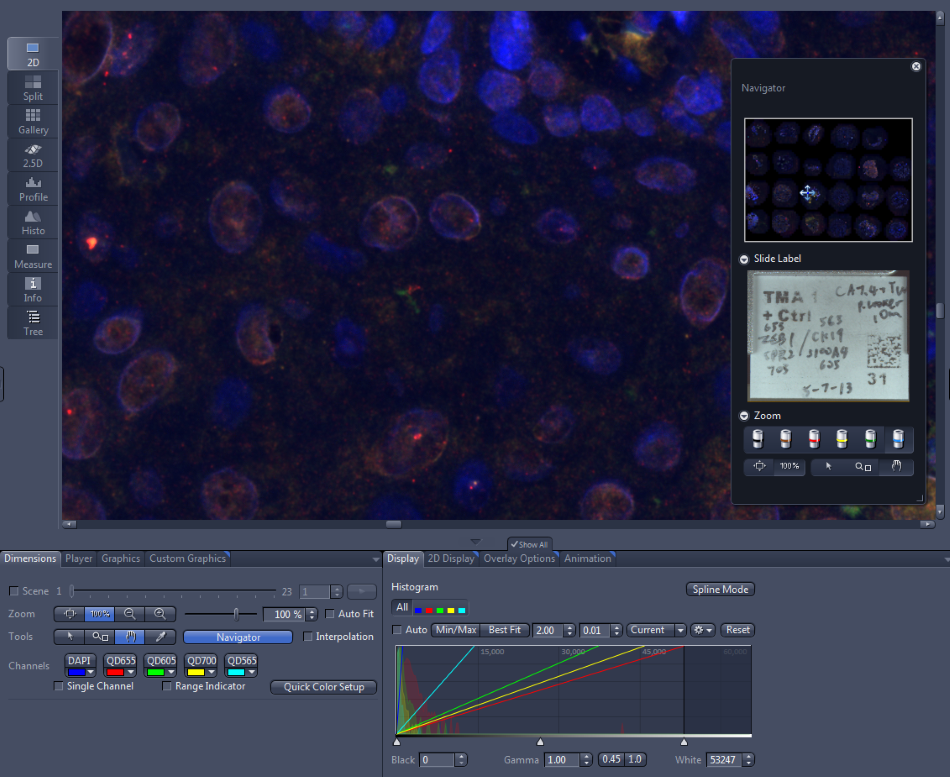
\includegraphics[width=\textwidth,height=\textheight/2,keepaspectratio=true]{ZEN_screenshot_1.PNG}
\doxyfigcaption{Z\+EN -\/ 2\+D-\/viewer}
\end{DoxyImage}
 The code is written in C++11 and (so far) has been successfully compiled with
\begin{DoxyItemize}
\item Visual Studio 2015 (Microsoft C++ v. 19.\+00.\+23506)
\item G\+CC 5.\+2.\+1 (on Ubuntu Linux 4.\+2.\+0)
\item Clang 3.\+4.\+1 (on Free\+B\+SD 10.\+2)
\end{DoxyItemize}

It is intended to be easily portable to other platforms.

It aims to be thread-\/safe (by most \href{https://en.wikipedia.org/wiki/Thread_safety}{\tt definitions}) -\/ which isn\textquotesingle{}t too surprising since it only allows read-\/only functionality. The library itself does not leverage multithreading, but it is designed for being used in a multithreaded environment.

\section*{C\+ZI in a nutshell }

Conceptionally a C\+Z\+I-\/document can be described as a set of blobs (or blocks -\/ in this context just a binary data structure defined only by its length), which are linked by a directory structure.


\begin{DoxyImage}
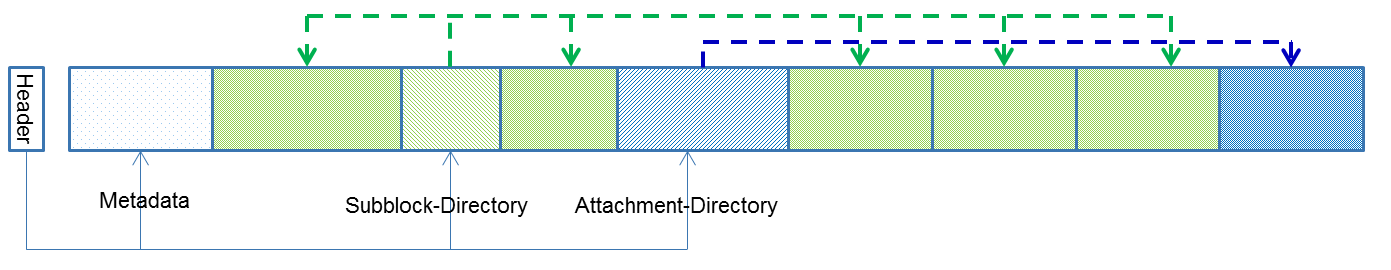
\includegraphics[width=\textwidth,height=\textheight/2,keepaspectratio=true]{CZI_1.PNG}
\doxyfigcaption{C\+ZI -\/ conceptual overview}
\end{DoxyImage}
 At the start of the file, there is a distinguished data-\/structure (\char`\"{}the header\char`\"{}) which (amongst other things) contains the offsets of three other special blocks\+:


\begin{DoxyItemize}
\item the metadata block (contains all \char`\"{}per document\char`\"{} metadata in X\+M\+L-\/format)
\item sub-\/block directory (contains a list of all sub-\/blocks contained in the document and their respective position in the file)
\item the attachment directory (contains a list of all attachment-\/blocks contained in the document and their respective position in the file)
\end{DoxyItemize}

With the term {\itshape sub-\/block} we are referring to an entity which contains a 2-\/dimensional image (or \char`\"{}a bitmap\char`\"{}), some associated metadata in X\+M\+L-\/format (which we refer to as {\itshape sub-\/block metadata}) and (potentially) some other binary attachment (referred to as {\itshape sub-\/block attachment}).~\newline
Do not confuse the terms \char`\"{}sub-\/block metadata\char`\"{}↔\char`\"{}metadata\char`\"{} and \char`\"{}sub-\/block attachment\char`\"{}↔\char`\"{}attachment\char`\"{} in this regard. Sub-\/blocks are identified by something like a coordinate -\/ a list of dimensions and for each dimension a value.

Attachments can contain any sort of binary data (their content is not further defined on the file-\/format level). They are identified by a string. A naming convention is used to discover their content.

The identifier (or coordinate) of a sub-\/block can be grouped in two categories\+: a number of abstract dimensions (abstract in the sense that the number is not directly related to a spatial point) and an X-\/\+Y-\/coordinate in a 2\+D-\/plane. Examples for the former are \char`\"{}\+C-\/dimension\char`\"{} (used for different channels) or \char`\"{}\+T-\/dimensions\char`\"{} (used for images acquired at different points in time) → \hyperlink{namespacelib_c_z_i_a55049658acf59d0eddfaebcad16df424}{cf. Dimension\+Index}. The X-\/\+Y-\/coordinate refer to a common (to all sub-\/blocks) coordinate system in which the sub-\/blocks are thought to be arranged. In fact -\/ sub-\/blocks are not only described by their X-\/\+Y-\/coordinate, but by a complete rectangle (adding witdth and height to the X-\/\+Y-\/coordinate) -\/ called the {\itshape logical rect}. And, in addition there is a parameter {\itshape physical width} and {\itshape physical height} → \hyperlink{structlib_c_z_i_1_1_sub_block_info}{cf. Sub\+Block\+Info}.~\newline
 
\begin{DoxyImage}
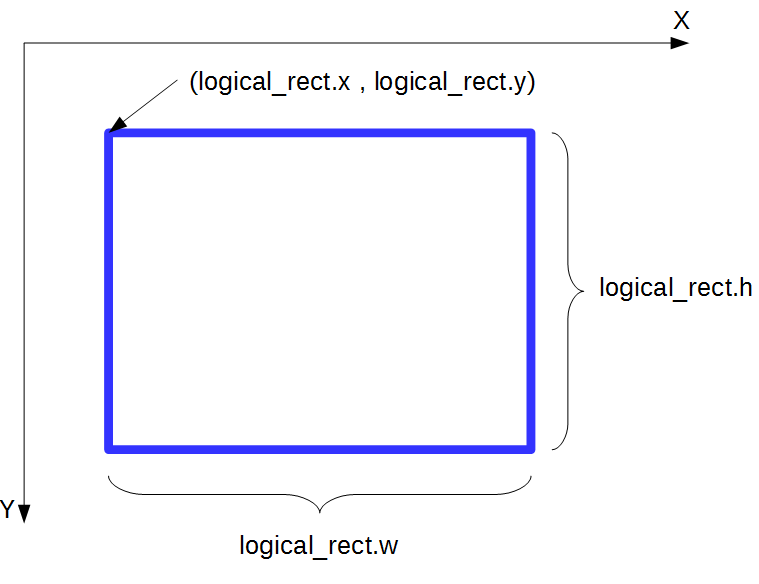
\includegraphics[width=\textwidth,height=\textheight/2,keepaspectratio=true]{CZI_2.PNG}
\doxyfigcaption{C\+ZI -\/ position of sub-\/block on plane}
\end{DoxyImage}
 So the logical\+\_\+rect defines the position (and size) of the sub-\/block on a plane. The physical\+\_\+size gives the width and height of the bitmap contained in the sub-\/block. They may or may not coincide with each other. If they do not coincide, then conceptually the bitmap is to be considered to have a different resolution -\/ so that we do not have a one-\/to-\/one correspondence between a pixel and an increment by 1 on the X-\/ or Y-\/coordinate. This concept is leveraged in order to have a resolution pyramid available in a C\+Z\+I-\/document. 
\chapter{Building lib\+C\+ZI}
\label{buildinglib_c_z_i}
\Hypertarget{buildinglib_c_z_i}
\hyperlink{namespacelib_c_z_i}{lib\+C\+ZI} aims to be portable and should build readily using a C++11 compiler. Here are some instructions for building on Windows and on Linux.

\subsection*{Building on Windows }

For Windows a solution-\/file (for Visual\+Studio 2015) {\ttfamily Lib\+C\+Z\+I-\/\+Solution} is provided.


\begin{DoxyImage}
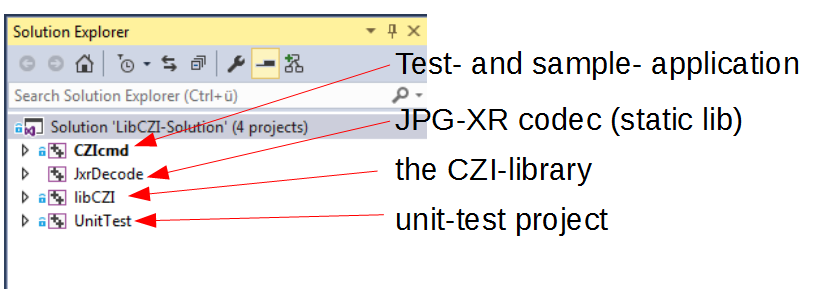
\includegraphics[width=\textwidth,height=\textheight/2,keepaspectratio=true]{VisualStudioProj_1.PNG}
\doxyfigcaption{lib\+C\+ZI solution}
\end{DoxyImage}
 We find these solution configurations and solution platforms defined\+:


\begin{DoxyImage}
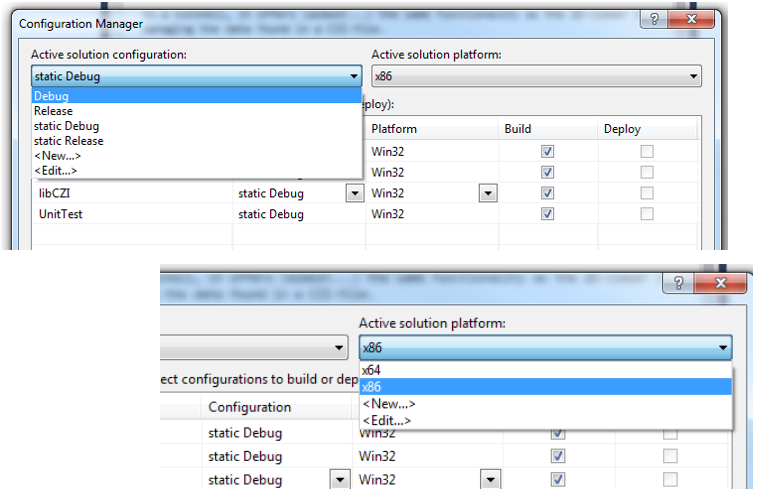
\includegraphics[height=10.8cm]{VisualStudioProj_2.PNG}
\doxyfigcaption{lib\+C\+ZI solution configurations/platforms}
\end{DoxyImage}


The configuration \char`\"{}static Debug\char`\"{} and \char`\"{}static Release\char`\"{} are configured to build a static lib\+C\+Z\+I-\/library (and link this static library e. g. in the project C\+Z\+Icmd). The configurations \char`\"{}\+Debug\char`\"{} and \char`\"{}\+Release\char`\"{} will create a dynamic link library lib\+C\+Z\+I.\+D\+LL (and C\+Z\+Icmd will consume this D\+LL). The \char`\"{}\+Unit\+Test\char`\"{} project can only be used with the \char`\"{}static\char`\"{} configurations, so it needs to be excluded from a batch-\/build\+:


\begin{DoxyImage}
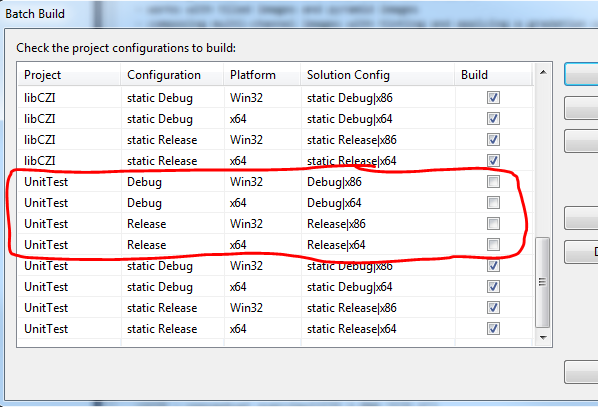
\includegraphics[height=10.8cm]{VisualStudioProj_3.PNG}
\doxyfigcaption{lib\+C\+ZI batch build}
\end{DoxyImage}


The projects are configured to put their results into these respective folders\+:


\begin{DoxyImage}
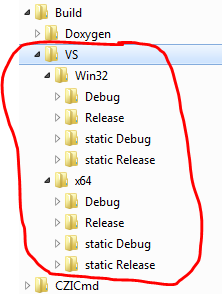
\includegraphics[width=\textwidth,height=\textheight/2,keepaspectratio=true]{VisualStudioProj_4.PNG}
\doxyfigcaption{build-\/targets folder layout}
\end{DoxyImage}
 After performing a build operation, you should find all build results there -\/ like shown here\+:


\begin{DoxyImage}
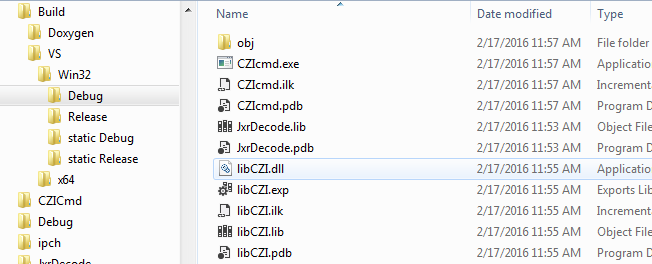
\includegraphics[width=\textwidth,height=\textheight/2,keepaspectratio=true]{VisualStudioProj_5.PNG}
\doxyfigcaption{build results}
\end{DoxyImage}
 \subsection*{Building on Linux }

For building on Linux, we are providing C\+Make-\/files. The C\+Make-\/files are very basic and minimal at this point, but should give you a working build.

In order to generate makefiles from the C\+Make-\/files, execute this command \begin{DoxyVerb}cmake -G "Unix Makefiles"
\end{DoxyVerb}



\begin{DoxyImage}
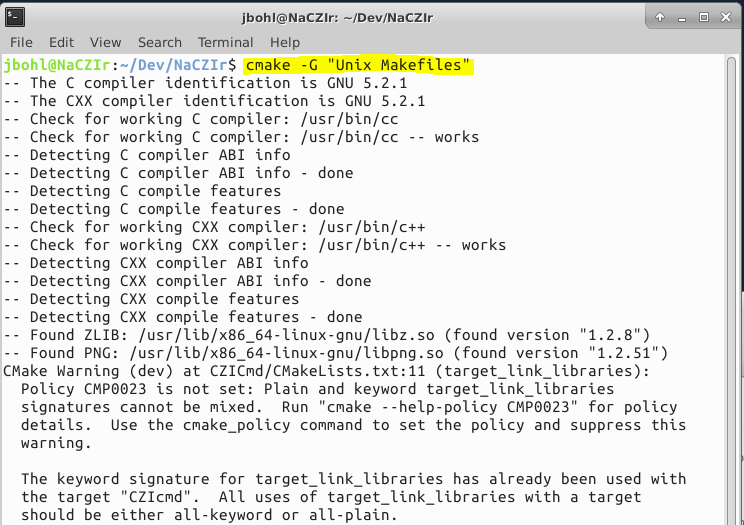
\includegraphics[width=\textwidth,height=\textheight/2,keepaspectratio=true]{LinuxBuild_1.PNG}
\doxyfigcaption{lib\+C\+ZI generate makefles with C\+Make}
\end{DoxyImage}
 Now executing a {\ttfamily make} command should produce a working binary\+:


\begin{DoxyImage}
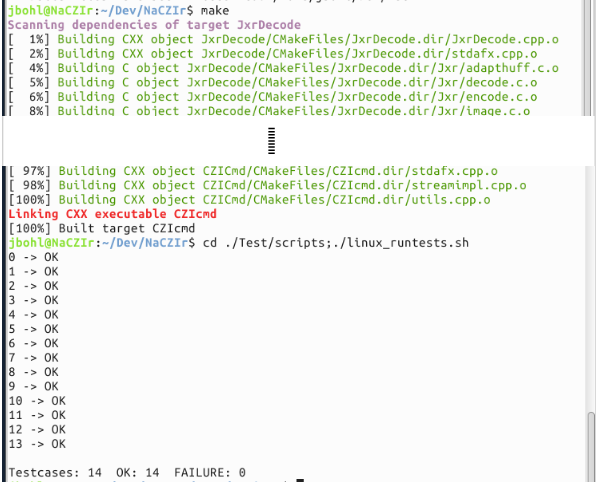
\includegraphics[width=\textwidth,height=\textheight/2,keepaspectratio=true]{LinuxBuild_2.PNG}
\doxyfigcaption{lib\+C\+ZI make}
\end{DoxyImage}


\subsection*{Building the documentation }

Executing {\ttfamily doxygen} will produce the documentation in this folder\+:


\begin{DoxyImage}
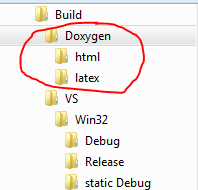
\includegraphics[width=\textwidth,height=\textheight/2,keepaspectratio=true]{doxygen_1.PNG}
\doxyfigcaption{lib\+C\+ZI doxygen}
\end{DoxyImage}
 In order to build the documentation in P\+D\+F-\/format, go into the folder ../\+Build/\+Doxygen/latex and execute {\ttfamily make}.~\newline
We had one issue with this\+: in order for the P\+D\+F-\/generation to succeed properly, we needed to make this change\+: in the file ../\+Build/\+Doxygen/latex/refman.tex (which is generated by the doxygen-\/run) find a line \begin{DoxyVerb}\usepackage[utf8]{inputenc}
\end{DoxyVerb}


and change it into \begin{DoxyVerb}\usepackage[utf8x]{inputenc}
\end{DoxyVerb}



\begin{DoxyImage}
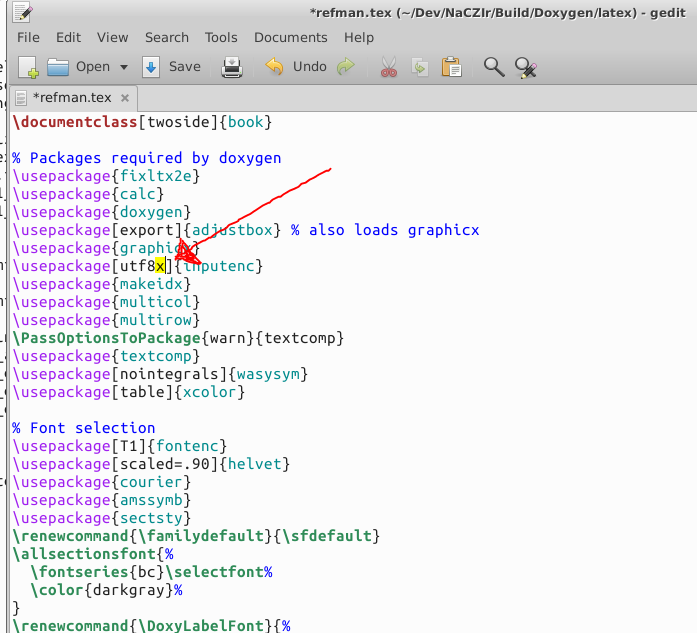
\includegraphics[width=\textwidth,height=\textheight/2,keepaspectratio=true]{doxygen_2.PNG}
\doxyfigcaption{fixing issue with P\+DF}
\end{DoxyImage}

\chapter{Image Document Concept}
\label{imagedocumentconcept}
\Hypertarget{imagedocumentconcept}
\subsection*{General concepts}

The sub-\/blocks contained in a C\+Z\+I-\/file are conceptually organized as follows\+:


\begin{DoxyItemize}
\item Sub-\/blocks reside in different \char`\"{}planes\char`\"{}, where a plane is given by the discrete coordinates \textquotesingle{}Z\textquotesingle{}, \textquotesingle{}C\textquotesingle{}, \textquotesingle{}T\textquotesingle{} or \textquotesingle{}V\textquotesingle{}.
\item Each sub-\/block has an X-\/Y coordinate (and a width and height) in a 2\+D-\/coordinate system (which is common to all planes).
\item Sub-\/blocks contain images which can be thought to fill an axis-\/aligned rectangle (specified by its X and Y coordinate, and its width and height).
\item In addition, a sub-\/block may have a logical size which is different from its physical size (also called a \char`\"{}zoom\char`\"{}).
\end{DoxyItemize}


\begin{DoxyImage}
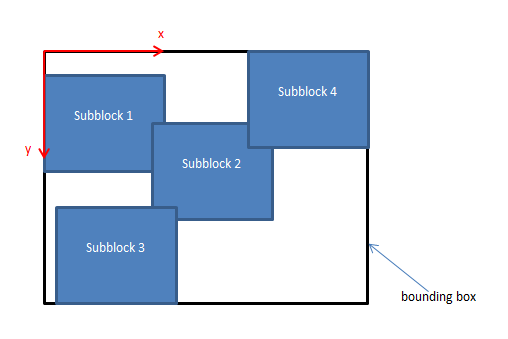
\includegraphics[width=\textwidth,height=\textheight/2,keepaspectratio=true]{image_document_concept1.PNG}
\doxyfigcaption{sub-\/blocks on a plane}
\end{DoxyImage}
 The case where we have different planes in one document is depicted here\+:


\begin{DoxyImage}
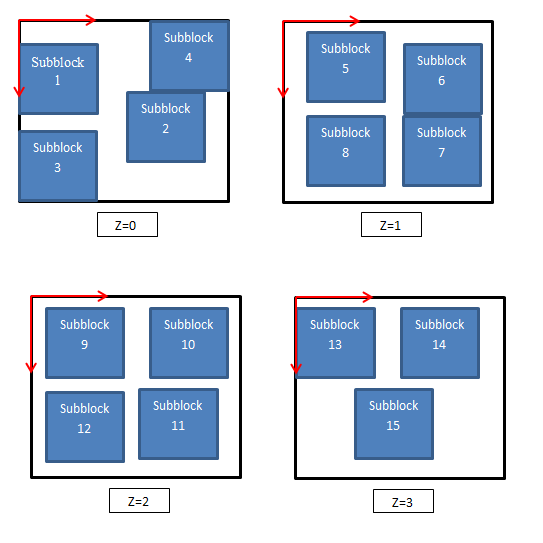
\includegraphics[width=\textwidth,height=\textheight/2,keepaspectratio=true]{image_document_concept2.PNG}
\doxyfigcaption{sub-\/blocks on different planes}
\end{DoxyImage}
 Note that\+:
\begin{DoxyItemize}
\item The X-\/Y positions of sub-\/blocks on different planes can be different (i. e. same Z-\/index, same T-\/index and same M-\/index does not imply that X and Y is the same for all C-\/indices). Even the number of sub-\/blocks on different planes can be different.
\item The bounding box is defined to contain all sub-\/blocks on all planes.
\item The 2\+D-\/coordinate system is common to all planes.
\item Sub-\/blocks can be overlapping.
\end{DoxyItemize}

\subsection*{Dimensions}

Each sub-\/blocks is labeled by a set of coordinates in different dimensions (the term \char`\"{}dimension\char`\"{} is used very loosely in the following discussion). We have already met the dimensions \textquotesingle{}Z\textquotesingle{}, \textquotesingle{}C\textquotesingle{}, \textquotesingle{}T\textquotesingle{} and \textquotesingle{}V\textquotesingle{} which are used to label different planes. In addition to them, a couple of more dimensions are in use\+:

\tabulinesep=1mm
\begin{longtabu} spread 0pt [c]{*{3}{|X[-1]}|}
\hline
\rowcolor{\tableheadbgcolor}\textbf{ dimension }&\textbf{ meaning }&\textbf{ comment  }\\\cline{1-3}
\endfirsthead
\hline
\endfoot
\hline
\rowcolor{\tableheadbgcolor}\textbf{ dimension }&\textbf{ meaning }&\textbf{ comment  }\\\cline{1-3}
\endhead
Z &z-\/focus &plane is from a different Z-\/plane \\\cline{1-3}
C &channel &different modality \\\cline{1-3}
T &time &different point in time \\\cline{1-3}
H &phase &distinguishes the different phases in a S\+I\+M-\/acquisition (structured illumination microscopy) \\\cline{1-3}
I &illumination &different directions of illumination (used in S\+P\+I\+M-\/acquisition) \\\cline{1-3}
V &view &used in S\+P\+IM for different views \\\cline{1-3}
\end{longtabu}
\textquotesingle{}H\textquotesingle{} and \textquotesingle{}I\textquotesingle{} have the character of an attribute in the sense that sub-\/blocks which differ only in the \textquotesingle{}H\textquotesingle{} (or \textquotesingle{}I\textquotesingle{}) coordinate must have the same X-\/\+Y-\/position in order to be meaningfull.

There is also the letter \textquotesingle{}M\textquotesingle{} in use for a dimension, but it has a somewhat different meaning. It is used in order to enumerate all tiles in a plane. I. e. all planes in a given plane shall have an M-\/index, and this M-\/index starts counting from zero to the number of tiles on that plane. The counting starts from zero for all different planes (and scenes). Tiles from different planes which differ in C are expected to have the same M-\/index (and, usually have the same X-\/\+Y-\/coordinate, but there are cases where the X-\/\+Y-\/coordinates are not exactly identical).

And we have the letter \textquotesingle{}S\textquotesingle{} in use, and it is used in the following way\+: sub-\/blocks with the same S-\/index form a set called \char`\"{}scene\char`\"{}. A scene is a rectangular (and axis aligned) region, and much like the bounding box, it is determined by taking all planes into consideration.


\begin{DoxyImage}
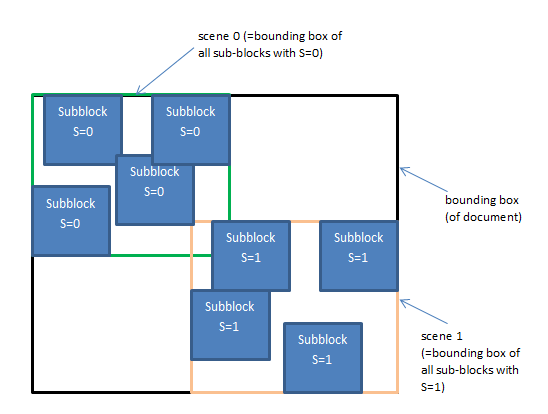
\includegraphics[width=\textwidth,height=\textheight/2,keepaspectratio=true]{image_document_concept3.PNG}
\doxyfigcaption{concept of scenes}
\end{DoxyImage}
 One restriction applies to scenes\+: scenes {\bfseries may} overlap, but sub-\/blocks (on pyramid-\/layer 0) belonging to different scenes {\bfseries must not} overlap.


\begin{DoxyImage}
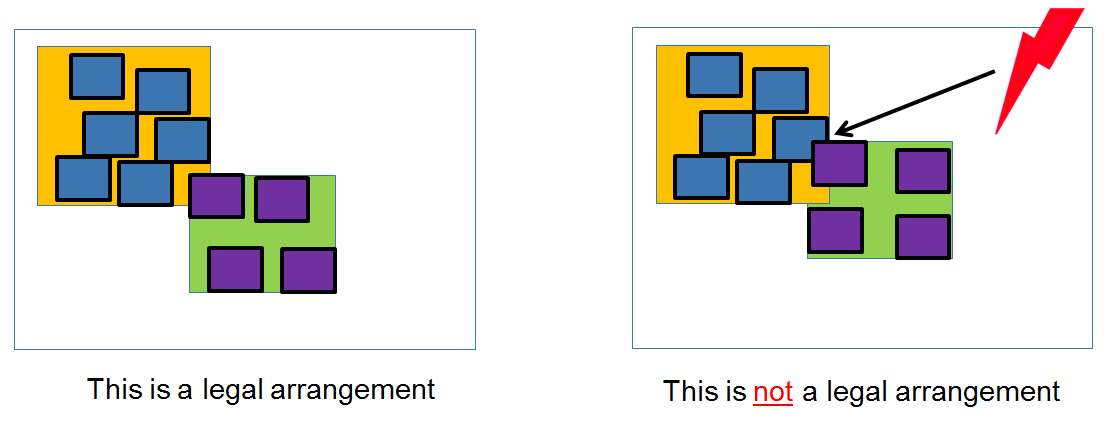
\includegraphics[width=\textwidth,height=\textheight/2,keepaspectratio=true]{image_document_concept4.PNG}
\doxyfigcaption{sub-\/block from different scenes must not overlap}
\end{DoxyImage}

\chapter{using lib\+C\+ZI}
\label{using_naczirlib}
\Hypertarget{using_naczirlib}
\subsection*{Opening a C\+Z\+I-\/file}

The first thing you want to do with a C\+Z\+I-\/file is to open it. This is done with the C\+Z\+I\+Reader-\/object. An instance of a C\+Z\+I\+Reader is created with the function


\begin{DoxyCode}
std::shared\_ptr<ICZIReader> \hyperlink{namespacelib_c_z_i_abe978d8bd50abe94c2d37df6212859e8}{CreateCZIReader}()
\end{DoxyCode}


The C\+Z\+I\+Reader-\/object has the following methods


\begin{DoxyCode}
\textcolor{keyword}{virtual} \textcolor{keywordtype}{void} Open(std::shared\_ptr<IStream> stream);
\textcolor{keyword}{virtual} std::shared\_ptr<IMetadataSegment> ReadMetadataSegment();
\textcolor{keyword}{virtual} std::shared\_ptr<IAccessor> CreateAccessor(AccessorType accessorType);
\textcolor{keyword}{virtual} \textcolor{keywordtype}{void} Close();

\textcolor{comment}{// ... some omitted}
\textcolor{keyword}{virtual} SubBlockStatistics GetStatistics();
\end{DoxyCode}


With the Open-\/method, the caller has to pass in an object which implements the interface \char`\"{}\+I\+Stream\char`\"{}. This object is used by the C\+Z\+I\+Reader in order to access the data in a C\+Z\+I-\/file. It is just the abstraction of a random-\/access stream. \hyperlink{namespacelib_c_z_i}{lib\+C\+ZI} includes a (simple) implementation for reading a file which is constructed by passing in a filename\+:


\begin{DoxyCode}
std::shared\_ptr<IStream> \hyperlink{namespacelib_c_z_i_a8783cf40c0eac418632db90c4f20b43b}{CreateStreamFromFile}(\textcolor{keyword}{const} \textcolor{keywordtype}{wchar\_t}* szFilename)
\end{DoxyCode}


When the Open-\/method has executed, the sub-\/block directory has been read and parsed, and the remaing methods can be called. This code can be used to open a C\+Z\+I-\/file\+:


\begin{DoxyCode}
\textcolor{keyword}{auto} stream = \hyperlink{namespacelib_c_z_i_a8783cf40c0eac418632db90c4f20b43b}{libCZI::CreateStreamFromFile}(LR\textcolor{stringliteral}{"(D:\(\backslash\)CZI\(\backslash\)sample.czi)");}
\textcolor{stringliteral}{}\textcolor{keyword}{auto} cziReader = \hyperlink{namespacelib_c_z_i_abe978d8bd50abe94c2d37df6212859e8}{libCZI::CreateCZIReader}();
cziReader->Open(stream); 
\end{DoxyCode}


The {\ttfamily Sub\+Block\+Statistics} gives information about the sub-\/blocks in the C\+Z\+I-\/file. The coordinates of each sub-\/block are examined, and the mininum and maximum are determined and are available in the struct returned by the method {\ttfamily I\+Sub\+Block\+Repository\+::\+Get\+Statistics()}. It is usually important to examine the dim\+Bounds member in order to determine which dimensions are used in the C\+Z\+I-\/file.

\subsection*{Reading sub-\/blocks in a C\+Z\+I-\/file}

All the sub-\/blocks in the C\+Z\+I-\/file can be enumerated by the method {\ttfamily I\+Sub\+Block\+Repository\+::\+Enumerate\+Sub\+Blocks}\+:


\begin{DoxyCode}
\textcolor{keyword}{virtual} \textcolor{keywordtype}{void} EnumerateSubBlocks(std::function<\textcolor{keywordtype}{bool}(\textcolor{keywordtype}{int} index, \textcolor{keyword}{const} SubBlockInfo& info)> funcEnum) 
\end{DoxyCode}


This code will print some of the information for all sub-\/blocks contained in a C\+Z\+I-\/file\+:


\begin{DoxyCode}
\textcolor{keyword}{auto} stream = \hyperlink{namespacelib_c_z_i_a8783cf40c0eac418632db90c4f20b43b}{libCZI::CreateStreamFromFile}(LR\textcolor{stringliteral}{"(W:\(\backslash\)Data\(\backslash\)TestData\(\backslash\)DCV\_30MB.czi)")
      ;}
\textcolor{stringliteral}{}\textcolor{keyword}{auto} cziReader = \hyperlink{namespacelib_c_z_i_abe978d8bd50abe94c2d37df6212859e8}{libCZI::CreateCZIReader}();
cziReader->Open(stream);
cziReader->EnumerateSubBlocks(
    [](\textcolor{keywordtype}{int} idx, \textcolor{keyword}{const} \hyperlink{structlib_c_z_i_1_1_sub_block_info}{libCZI::SubBlockInfo}& info)
\{
    cout << \textcolor{stringliteral}{"Index "} << idx << \textcolor{stringliteral}{": "} << \hyperlink{classlib_c_z_i_1_1_utils_aeb42843e65615302b51b68ad2b376e6d}{libCZI::Utils::DimCoordinateToString}
      (&info.\hyperlink{structlib_c_z_i_1_1_sub_block_info_ae4acf2922fe594327d1c6fbfb2062781}{coordinate}) << \textcolor{stringliteral}{" Rect="} << info.logigalRect << endl;
    \textcolor{keywordflow}{return} \textcolor{keyword}{true};
\});
\end{DoxyCode}


It will print out something like\+: \begin{DoxyVerb}...
Index 4: Z4C0T0 Rect=(0,0,512,512)
Index 5: Z5C0T0 Rect=(0,0,512,512)
Index 6: Z6C0T0 Rect=(0,0,512,512)
Index 7: Z7C0T0 Rect=(0,0,512,512)
Index 8: Z8C0T0 Rect=(0,0,512,512)
Index 9: Z9C0T0 Rect=(0,0,512,512)
Index 10: Z10C0T0 Rect=(0,0,512,512)
Index 11: Z11C0T0 Rect=(0,0,512,512)
Index 12: Z12C0T0 Rect=(0,0,512,512)
Index 13: Z13C0T0 Rect=(0,0,512,512)
Index 14: Z14C0T0 Rect=(0,0,512,512)
...
\end{DoxyVerb}


The index argument we got here is used to identify a sub-\/block and can be used with the method {\ttfamily I\+Sub\+Block\+Repository\+::\+Read\+Sub\+Block}. This code will enumerate all sub-\/blocks found in a C\+Z\+I-\/file, read them and save them to a P\+N\+G-\/file\+:


\begin{DoxyCode}
\textcolor{keyword}{auto} stream = \hyperlink{namespacelib_c_z_i_a8783cf40c0eac418632db90c4f20b43b}{libCZI::CreateStreamFromFile}(LR\textcolor{stringliteral}{"(W:\(\backslash\)Data\(\backslash\)TestData\(\backslash\)DCV\_30MB.czi)")
      ;}
\textcolor{stringliteral}{}\textcolor{keyword}{auto} cziReader = \hyperlink{namespacelib_c_z_i_abe978d8bd50abe94c2d37df6212859e8}{libCZI::CreateCZIReader}();
cziReader->Open(stream);
cziReader->EnumerateSubBlocks(
    [&](\textcolor{keywordtype}{int} idx, \textcolor{keyword}{const} \hyperlink{structlib_c_z_i_1_1_sub_block_info}{libCZI::SubBlockInfo}& info)
\{
    \textcolor{keyword}{auto} sbBlk = cziReader->ReadSubBlock(idx);
    \textcolor{keyword}{auto} bitmap = sbBlk->CreateBitmap();
    wstring filename(L\textcolor{stringliteral}{"SubBlock#"});
    filename += to\_wstring(idx);
    filename += L\textcolor{stringliteral}{".PNG"};
    SaveAsPng(filename, bitmap);
    \textcolor{keywordflow}{return} \textcolor{keyword}{true};
\});
\end{DoxyCode}


Note that the function {\ttfamily Save\+As\+Png} is not part of \hyperlink{namespacelib_c_z_i}{lib\+C\+ZI}. It is also worth noting that the {\ttfamily I\+Sub\+Block\+::\+Create\+Bitmap} method will transparently decode the bitmap (in case we have a compressed bitmap in the sub-\/block).

\subsection*{creating multi-\/tile composites}

This piece of code will extract a small rectangular region from a huge multi-\/tile document\+:


\begin{DoxyCode}
\textcolor{keyword}{auto} stream = \hyperlink{namespacelib_c_z_i_a8783cf40c0eac418632db90c4f20b43b}{libCZI::CreateStreamFromFile}(LR\textcolor{stringliteral}{"(
      D:\(\backslash\)PICTURES\(\backslash\)NaCZIrTestData\(\backslash\)Example\_TMA1\_Zeb1\_SPRR2\_Ck19\_S100-1-1-1-1.czi)");}
\textcolor{stringliteral}{}\textcolor{keyword}{auto} cziReader = \hyperlink{namespacelib_c_z_i_abe978d8bd50abe94c2d37df6212859e8}{libCZI::CreateCZIReader}();
cziReader->Open(stream);
\textcolor{keyword}{auto} statistics = cziReader->GetStatistics();
\textcolor{keyword}{auto} accessor = cziReader->CreateSingleChannelTileAccessor();
\hyperlink{classlib_c_z_i_1_1_c_dim_coordinate}{libCZI::CDimCoordinate} planeCoord\{ \{ NaCZIr::DimensionIndex::C,1 \} \};   \textcolor{comment}{// the
       document only contains C-dimension}
\textcolor{keyword}{auto} multiTileComposit = accessor->Get(
    \hyperlink{structlib_c_z_i_1_1_int_rect}{libCZI::IntRect}\{ statistics.boundingBox.\hyperlink{structlib_c_z_i_1_1_int_rect_a7a1e25fc9f6a4c99d9a3710446b7a5de}{x} + 26152, statistics.boundingBox.y + 32215 ,
      3000,2200 \},
    &planeCoord,
    \textcolor{keyword}{nullptr});   \textcolor{comment}{// use default options}
SaveAsPng(LR\textcolor{stringliteral}{"(D:\(\backslash\)TileComposite.png)", multiTileComposit);}
\end{DoxyCode}


Note that we are using the {\ttfamily Sub\+Block\+Statistics} in order to specify a R\+OI with coordinates relative to the upper left corner of the bounding box. The result is depicted here\+:


\begin{DoxyImage}
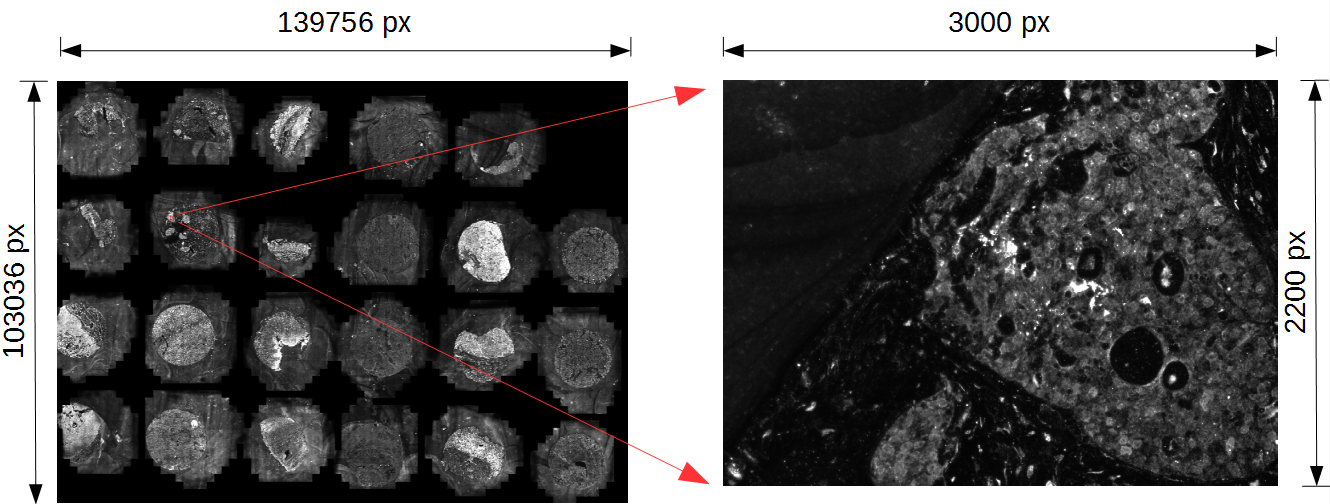
\includegraphics[width=\textwidth,height=\textheight/2,keepaspectratio=true]{SingleChannelTileAccessor_3.PNG}
\doxyfigcaption{single channel tile accessor}
\end{DoxyImage}


Here is an example which leverages the Single\+Channel\+Scaling\+Tile\+Accessor\+:


\begin{DoxyCode}
\textcolor{keyword}{auto} stream = \hyperlink{namespacelib_c_z_i_a8783cf40c0eac418632db90c4f20b43b}{libCZI::CreateStreamFromFile}(LR\textcolor{stringliteral}{"(
      D:\(\backslash\)PICTURES\(\backslash\)NaCZIrTestData\(\backslash\)Example\_TMA1\_Zeb1\_SPRR2\_Ck19\_S100-1-1-1-1.czi)");}
\textcolor{stringliteral}{}\textcolor{keyword}{auto} cziReader = \hyperlink{namespacelib_c_z_i_abe978d8bd50abe94c2d37df6212859e8}{libCZI::CreateCZIReader}();
cziReader->Open(stream);
\textcolor{keyword}{auto} statistics = cziReader->GetStatistics();
\textcolor{keyword}{auto} accessor = cziReader->CreateSingleChannelScalingTileAccessor();
NaCZIr::CDimCoordinate planeCoord\{ \{ \hyperlink{namespacelib_c_z_i_a55049658acf59d0eddfaebcad16df424a0d61f8370cad1d412f80b84d143e1257}{libCZI::DimensionIndex::C},1 \} \}; \textcolor{comment}{// the
       document only contains C-dimension, we choose channel#1}
\textcolor{keyword}{auto} multiTileComposit = accessor->Get(
    \hyperlink{structlib_c_z_i_1_1_int_rect}{libCZI::IntRect}\{
            statistics.boundingBox.\hyperlink{structlib_c_z_i_1_1_int_rect_a7a1e25fc9f6a4c99d9a3710446b7a5de}{x} + statistics.boundingBox.w / 4,
            statistics.boundingBox.y + statistics.boundingBox.h / 4 ,
            (statistics.boundingBox.w / 8) * 5,
            (statistics.boundingBox.h / 8) * 5 \},
    &planeCoord,
    0.1f,
    \textcolor{keyword}{nullptr});
SaveAsPng(LR\textcolor{stringliteral}{"(D:\(\backslash\)ScalingTileComposite.png)", multiTileComposit);}
\end{DoxyCode}


The R\+OI is now x= $\frac{width}{4}$, y= $\frac{height}{4}$, w= $\frac{5}{8}\cdot width$, h= $\frac{5}{8}\cdot height$ -\/ where $width$ and $height$ refer to the width and height of the bounding box of the document. ~\newline
The zoom is given as 0.\+1 -\/ so the resulting document will have width= $0.1\times\frac{5}{8}\cdot width$ and height=width= $0.1\times\frac{5}{8}\cdot height$.

This operaton is depicted here\+:


\begin{DoxyImage}
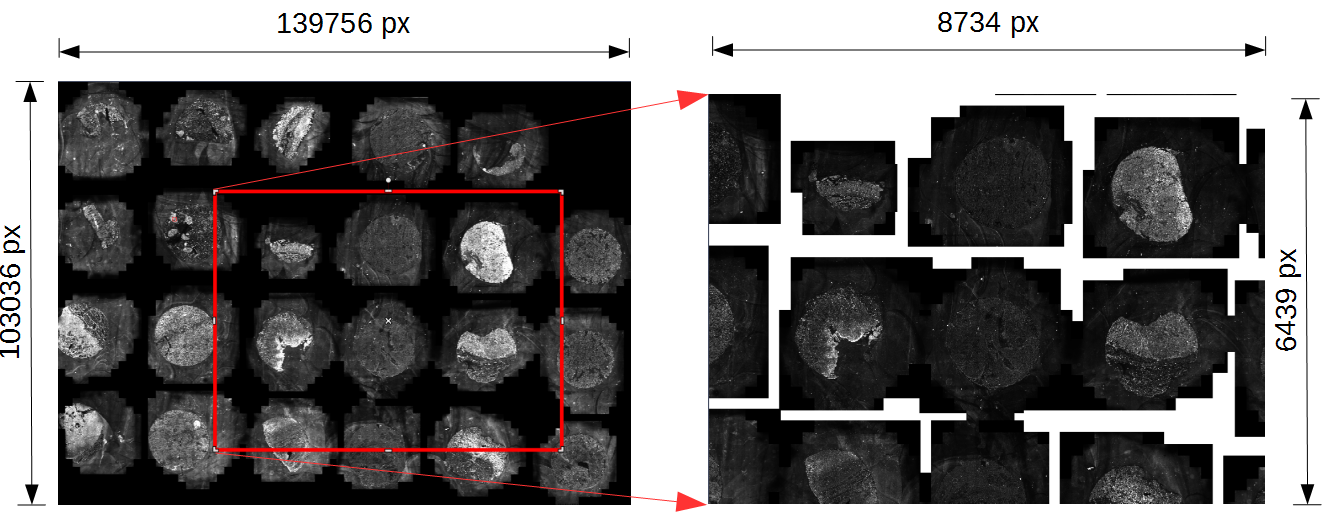
\includegraphics[width=\textwidth,height=\textheight/2,keepaspectratio=true]{SingleChannelTileAccessor_4.PNG}
\doxyfigcaption{single channel scaling tile accessor}
\end{DoxyImage}
 \subsection*{creating a multi-\/channel composite}

In order to create a colorful picture from a bunch of channels (usually grayscale), we need to apply a color to it -\/ that\textquotesingle{}s refered to as \char`\"{}tinting\char`\"{}. Furthermore, we want to apply a gradation curve. All the required parameters for this are refered to as \char`\"{}display settings\char`\"{}. In a C\+Z\+I-\/file we can find display settings in the metadata. The following sample is reading the display settings from the metadata; then we get a (scaled) multi-\/tile composite for each of the channels (more exactly\+: only for those channels which are marked \textquotesingle{}active\textquotesingle{} in the display settings). Those bitmaps are then fed into a function which will produce the multi-\/channel-\/composite (according to the display settings).


\begin{DoxyCode}
\textcolor{keyword}{auto} stream = \hyperlink{namespacelib_c_z_i_a8783cf40c0eac418632db90c4f20b43b}{libCZI::CreateStreamFromFile}(LR\textcolor{stringliteral}{"(
      D:\(\backslash\)PICTURES\(\backslash\)NaCZIrTestData\(\backslash\)Example\_TMA1\_Zeb1\_SPRR2\_Ck19\_S100-1-1-1-1.czi)");}
\textcolor{stringliteral}{}\textcolor{keyword}{auto} cziReader = \hyperlink{namespacelib_c_z_i_abe978d8bd50abe94c2d37df6212859e8}{libCZI::CreateCZIReader}();
cziReader->Open(stream);
\textcolor{keyword}{auto} statistics = cziReader->GetStatistics();

\textcolor{comment}{// get the display-setting from the document's metadata}
\textcolor{keyword}{auto} mds = cziReader->ReadMetadataSegment();
\textcolor{keyword}{auto} md = mds->CreateMetaFromMetadataSegment();
\textcolor{keyword}{auto} docInfo = md->GetDocumentInfo();
\textcolor{keyword}{auto} dsplSettings = docInfo->GetDisplaySettings();

\hyperlink{structlib_c_z_i_1_1_int_rect}{libCZI::IntRect} roi\{
    statistics.boundingBox.\hyperlink{structlib_c_z_i_1_1_int_rect_a7a1e25fc9f6a4c99d9a3710446b7a5de}{x} + statistics.boundingBox.w / 4,
    statistics.boundingBox.y + statistics.boundingBox.h / 4 ,
    (statistics.boundingBox.w / 8) * 5, (statistics.boundingBox.h / 8) * 5 \};

\textcolor{comment}{// get the tile-composite for all channels (which are marked 'active' in the display-settings)}
std::vector<shared\_ptr<libCZI::IBitmapData>> actvChBms;
\textcolor{keywordtype}{int} index = 0;  \textcolor{comment}{// index counting only the active channels}
std::map<int, int> activeChNoToChIdx;   \textcolor{comment}{// we need to keep track which 'active channels" corresponds to
       which channel index}
\textcolor{keyword}{auto} accessor = cziReader->CreateSingleChannelScalingTileAccessor();
libCZI::CDisplaySettingsHelper::EnumEnabledChannels(dsplSettings.get(),
    [&](\textcolor{keywordtype}{int} chIdx)->\textcolor{keywordtype}{bool}
\{
    \hyperlink{classlib_c_z_i_1_1_c_dim_coordinate}{libCZI::CDimCoordinate} planeCoord\{ \{ 
      \hyperlink{namespacelib_c_z_i_a55049658acf59d0eddfaebcad16df424a0d61f8370cad1d412f80b84d143e1257}{libCZI::DimensionIndex::C}, chIdx \} \};
    actvChBms.emplace\_back(accessor->Get(roi, &planeCoord, 0.05f, \textcolor{keyword}{nullptr}));
    activeChNoToChIdx[chIdx] = index++;
    \textcolor{keywordflow}{return} \textcolor{keyword}{true};
\});

\textcolor{comment}{// initialize the helper with the display-settings and provide the pixeltypes }
\textcolor{comment}{// (for each active channel)}
libCZI::CDisplaySettingsHelper dsplHlp;
dsplHlp.Initialize(dsplSettings.get(), 
    [&](\textcolor{keywordtype}{int} chIdx)->\hyperlink{namespacelib_c_z_i_abf8ce12ab88b06c8b3b47efbb5e2e834}{libCZI::PixelType} \{ \textcolor{keywordflow}{return} actvChBms[activeChNoToChIdx[chIdx]]->
      GetPixelType(); \});

\textcolor{comment}{// pass the tile-composites we just created (and the display-settings for the those active }
\textcolor{comment}{//  channels) into the multi-channel-composor-function}
\textcolor{keyword}{auto} mcComposite = \hyperlink{classlib_c_z_i_1_1_compositors_ab9be96d1b2b2e48c60c4dbf967e593c1}{libCZI::Compositors::ComposeMultiChannel\_Bgr24}
      (
    dsplHlp.GetActiveChannelsCount(),
    std::begin(actvChBms),
    dsplHlp.GetChannelInfosArray());

SaveAsPng(LR\textcolor{stringliteral}{"(D:\(\backslash\)ScalingTileComposite\_MultiChannelComposite.png)", mcComposite);}
\end{DoxyCode}


In this sample we used the same document and R\+OI as before. The C\+Z\+I-\/file in this case contained 5 channels (and all being \textquotesingle{}active\textquotesingle{}), so we had to get 5 tile-\/composites (using the Single\+Channel\+Scaling\+Tile\+Accessor), which are then all put into the {\ttfamily Compose\+Multi\+Channel\+\_\+\+Bgr24} function (alongside with the corresponding display-\/settings). The function will produce a new bitmap (always of pixeltype Bgr24) which then contains the multi-\/channel-\/composite image. In this process we leveraged a utility {\ttfamily C\+Display\+Settings\+Helper} which hides some of the book-\/keeping (among other things, it helps sorting out the \textquotesingle{}active\textquotesingle{} channels and it converts the display-\/settings we got from the document\textquotesingle{}s metadata into the form expected by the {\ttfamily Compose\+Multi\+Channel\+\_\+\+Bgr24} function).

The complete operation is depicted here\+:


\begin{DoxyImage}
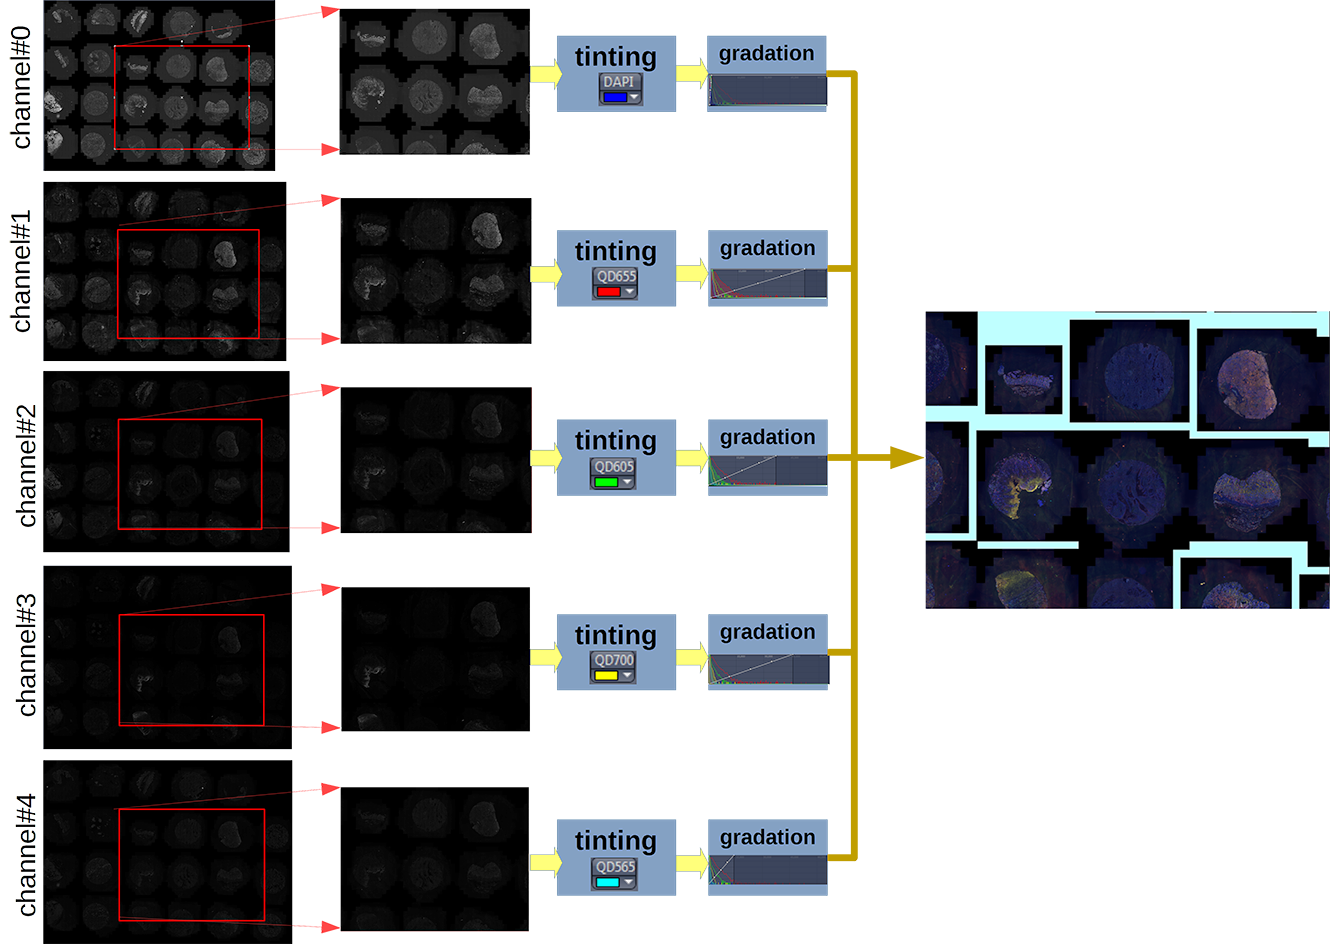
\includegraphics[width=\textwidth,height=\textheight/2,keepaspectratio=true]{ScalingSingleChannelTileAccessor1.png}
\doxyfigcaption{multi-\/channel-\/composite from a (scaled) tile-\/composite}
\end{DoxyImage}
 
\chapter{Accessors}
\label{accessors}
\Hypertarget{accessors}
The bitmaps from the individual sub-\/blocks are logically arranged as tiles on a plane. In order to get a bitmap containing the tile-\/composite (or a part of it) the use of a accessor is required. In this example, we have three tiles on a plane and request to get a certain section (aka region-\/of-\/interest R\+OI)\+:


\begin{DoxyImage}
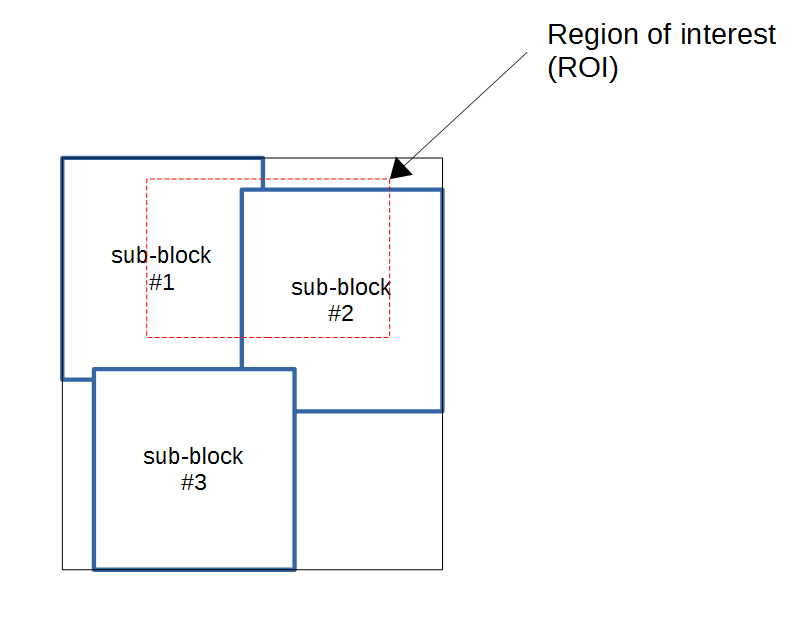
\includegraphics[width=\textwidth,height=\textheight/2,keepaspectratio=true]{compositors_1.png}
\doxyfigcaption{multi-\/tile accessor\+: mode of operation}
\end{DoxyImage}
 The resulting bitmap in this case will look like this\+:


\begin{DoxyImage}
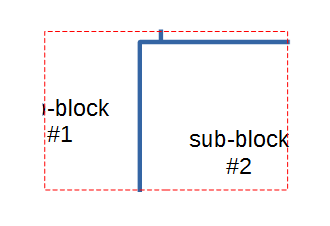
\includegraphics[width=\textwidth,height=\textheight/2,keepaspectratio=true]{compositors_2.png}
\doxyfigcaption{multi-\/tile composit}
\end{DoxyImage}


When creating the output bitmap, the pixels are converted to the destination pixeltype (if necessary). This conversion is done in the following way\+:

\tabulinesep=1mm
\begin{longtabu} spread 0pt [c]{*{3}{|X[-1]}|}
\hline
\rowcolor{\tableheadbgcolor}\textbf{ source pixel type }&\textbf{ destination pixel type }&\textbf{ operation  }\\\cline{1-3}
\endfirsthead
\hline
\endfoot
\hline
\rowcolor{\tableheadbgcolor}\textbf{ source pixel type }&\textbf{ destination pixel type }&\textbf{ operation  }\\\cline{1-3}
\endhead
Gray8 &B\+G\+R24 &R8 = G8 = B8 ← Gray8 \\\cline{1-3}
Gray8 &B\+G\+R48 &R8 = G8 = B8 ← Gray8 \\\cline{1-3}
Gray16 &B\+G\+R24 &R8 = G8 = B8 ← Gray16/256 \\\cline{1-3}
Gray16 &B\+G\+R48 &R8 = G8 = B8 ← Gray16 \\\cline{1-3}
B\+G\+R24 &Gray8 &Gray8 ← $ \frac{R8+G8+B8}{3} $ \\\cline{1-3}
B\+G\+R48 &Gray8 &Gray8 ← $ (\frac{R16}{256}+\frac{G16}{256}+\frac{B16}{256})/3 $ \\\cline{1-3}
Gray8 &Gray16 &Gray8 ← Gray16/256 \\\cline{1-3}
R\+G\+B24 &R\+G\+B48 &R16 ← R8, G16 ← G8, B16 ← B8 \\\cline{1-3}
R\+G\+B48 &R\+G\+B24 &R8 ← $\frac{R16}{256}$, G16 ← $\frac{G16}{256}$, B16 ← $\frac{B16}{256}$ \\\cline{1-3}
\end{longtabu}
We have three types of accessors available\+:

\tabulinesep=1mm
\begin{longtabu} spread 0pt [c]{*{2}{|X[-1]}|}
\hline
\rowcolor{\tableheadbgcolor}\textbf{ accessor }&\textbf{ purpose  }\\\cline{1-2}
\endfirsthead
\hline
\endfoot
\hline
\rowcolor{\tableheadbgcolor}\textbf{ accessor }&\textbf{ purpose  }\\\cline{1-2}
\endhead
Single\+Channel\+Tile\+Accessor &get a multi-\/tile composite only from pyramid-\/layer 0 \\\cline{1-2}
Single\+Channel\+Pyramid\+Layer\+Tile\+Accessor &get a multi-\/tile composite from an explictly specified pyramid-\/layer \\\cline{1-2}
Single\+Channel\+Scaling\+Tile\+Accessor &get a multi-\/tile composite at an arbitrary zoom-\/level \\\cline{1-2}
\end{longtabu}
The Single\+Channel\+Tile\+Accessor will only operate on tiles on pyramid-\/level 0 -\/ i.\+e. only on sub-\/blocks for which physical\+\_\+size = logical\+\_\+size. The size (in pixels) of the resulting multi-\/tile-\/composit is the same as the R\+OI specified.

The Single\+Channel\+Pyramid\+Layer\+Tile\+Accessor allows to access a specific pyramid-\/level. But it will only consider sub-\/blocks from this pyramd-\/level when composing the tile-\/composite.

The Single\+Channel\+Scaling\+Tile\+Accessor allows to specify an arbitrary zoom-\/level, it will choose the appropriate pyramid-\/level and scale the bitmaps (if necessary) to fit the desired zoom-\/level. 
\chapter{Multi-\/channel-\/composition}
\label{multichannelcomposition}
\Hypertarget{multichannelcomposition}
Multi-\/channel-\/composition is the operation of combining a set of channels (usually grayscale images) into a one colored image.

The operation (as implemented by the function Compositors\+::\+Compose\+Multi\+Channel) is controlled by the following options\+:


\begin{DoxyItemize}
\item tinting by a color
\item definition of a black-\/ and white-\/point
\item a gradiation curve
\end{DoxyItemize}

The steps in the operation are\+: \begin{DoxyVerb}Let result R-G-B pixel value = 0,0,0
For each channel  
    If tinting is enabled for this channel:
        - get normalized pixel value
        - apply gradation
        - multiply with R-G-B tinting color
        - add R-G-B value to result pixel 

    If tinting is disabled for this channel:
        - get normalized R-G-B value
        - apply gradation to R, G and B
        - add R-G-B value to result pixel 
\end{DoxyVerb}


The operation \char`\"{}\+Apply gradiation\char`\"{} works in the following way\+: the normalized pixel value is mapped to an integer (in the range 0..255) by looking up a value\+:


\begin{DoxyImage}
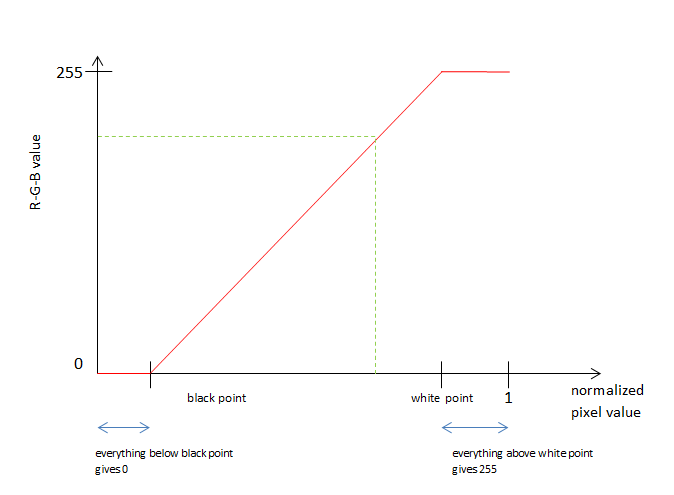
\includegraphics[width=\textwidth,height=\textheight/2,keepaspectratio=true]{gradationcurve_1.PNG}
\doxyfigcaption{linear gradation curve}
\end{DoxyImage}
 Above a linear gradation curve is shown. There are three ways commonly used to define the gradation curve\+:
\begin{DoxyItemize}
\item linear (a straight line from the point \mbox{[}black point,0\mbox{]} to \mbox{[}white point,255\mbox{]} -\/ as shown above)
\item gamma (instead of a straight line we use an exponential with the exponent gamma as a parameter)
\item defined by a spline
\end{DoxyItemize}

In the function Compositors\+::\+Compose\+Multi\+Channel the gradation curve is given as an array of bytes. Those bytes give the R\+G\+B-\/value at uniformly distributed points between black point and white point. Values between those points are interpolated linearly.

For example, the parameters white\+\_\+point=0.\+2, black\+\_\+point=1.\+0 and lookup\+Table=\{0, 66, 100, 166, 255\} will result in this gradation curve\+:


\begin{DoxyImage}
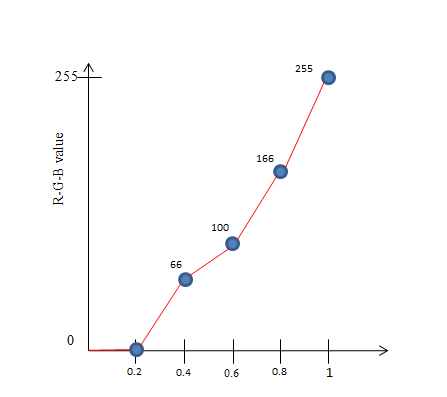
\includegraphics[width=\textwidth,height=\textheight/2,keepaspectratio=true]{gradationcurve_2.PNG}
\doxyfigcaption{gradation curve sample}
\end{DoxyImage}
 For generating a look-\/up-\/table (which then can be used for Compositors\+::\+Compose\+Multi\+Channel) two utility functions are provided\+: Utils\+::\+Create8\+Bit\+Look\+Up\+Table\+From\+Splines and Utils\+::\+Create8\+Bit\+Look\+Up\+Table\+From\+Gamma. 
\chapter{C\+Z\+Icmd Documentation}
\label{naczircmd}
\Hypertarget{naczircmd}
The console application \char`\"{}\+C\+Z\+Icmd\char`\"{} is provided for two purposes\+:
\begin{DoxyItemize}
\item demonstrate the usage of the \hyperlink{namespacelib_c_z_i}{lib\+C\+ZI}
\item it might be useful to convert/extract data from a C\+Z\+I-\/file
\end{DoxyItemize}

The parameters of the program are\+: \begin{DoxyVerb}usage: CZIcmd -c COMMAND -s SOURCEFILE -o OUTPUTFILE [-p PLANECOORDINATE]
                 [-r ROI] [-d DISPLAYSETTINGS] [-h] [-b] [-t] [-j DECODERNAME] 
                 [-v VERBOSITYLEVEL] [-y PYRAMIDINFO] [-z ZOOM] [-i INFOLEVEL]
                 [-e SELECTION] [-f FILTER]

  using libCZI version 0.2

  -?, --help          Show this help message and exit.
  -c COMMAND, --command COMMAND
                      COMMAND can be any of 'PrintInformation',
                      'ExtractSubBlock', 'SingleChannelTileAccessor',
                      'ChannelComposite', 'SingleChannelPyramidTileAccessor',
                      'SingleChannelScalingTileAccessor',
                      'ScalingChannelComposite' and 'ExtractAttachment'.
                      'PrintInformation' will print information about the
                      CZI-file to the console. The argument 'info-level' can be
                      used to specify which information is to be printed.
                      'ExtractSubBlock' will write the bitmap contained in the
                      specified sub-block to the OUTPUTFILE.
                      'ChannelComposite' will create a channel-composite of the
                      specified region and plane and apply display-settings to
                      it. The resulting bitmap will be written to the specified
                      OUTPUTFILE.
                      'SingleChannelTileAccessor' will create a tile-composite
                      (only from sub-blocks on pyramid-layer 0) of the
                      specified region and plane. The resulting bitmap will be
                      written to the specified OUTPUTFILE.
                      'SingleChannelPyramidTileAccessor' adds to the previous
                      command the ability to explictely address a specific
                      pyramid-layer (which must exist in the CZI-document).
                      'SingleChannelScalingTileAccessor' gets the specified
                      region with an arbitrary zoom factor. It uses the
                      pyramid-layers in the CZI-document and scales the bitmap
                      if neccessary. The resulting bitmap will be written to
                      the specified OUTPUTFILE.
                      'ScalingChannelComposite' operates like the previous
                      command, but in addition gets all channels and creates a
                      multi-channel-composite from them using display-settings.
                      'ExtractAttachment' allows to extract (and save to a
                      file) the contents of attachments.
  -s SOURCEFILE, --source SOURCEFILE
                      SOURCEFILE specifies the source CZI-file.
  -o OUTPUTFILE, --output OUTPUTFILE
                      OUTPUTFILE specifies the output-filename. A suffix will
                      be appended to the name given here depending on the type
                      of the file.
  -p PLANE-COORDINATES, --plane-coordinate PLANE-COORDINATES
                      Uniquely select a 2D-plane from the document. It is given
                      in the form [DimChar][number], where 'DimChar' specifies
                      a dimension and can be any of 'Z', 'C', 'T', 'R', 'I',
                      'H', 'V' or 'B'. 'number' is an integer.
                      Examples: C1T3, C0T-2, C1T44Z15H1.
  -r ROI, --rect ROI
                      Select a paraxial rectangular region as the
                      region-of-interest. The coordinates may be given either
                      absolute or relative. If using relative coordinates, they
                      are relative to what is determined as the upper-left
                      point in the document.
                      Relative coordinates are specified with the syntax
                      'rel([x],[y],[width],[height])', absolute coordinates are
                      specified 'abs([x],[y],[width],[height])'.
                      Examples: rel(0,0,1024,1024), rel(-100,-100,500,500),
                      abs(-230,100,800,800).
  -d DISPLAYSETTINGS, --display-settings DISPLAYSETTINGS
                      Specifies the display-settings used for creating a
                      channel-composite. The data is given in JSON-notation.
  -h, --calc-hash     Calculate a hash for the output-picture. The
                      MD5Sum-algorithm is used for this.
  -t, --drawtileboundaries
  -j DECODERNAME, --jpgxrcodec DECODERNAME
                      Choose which decoder implementation is used. Specifying
                      "WIC" will request the Windows-provided decoder - which
                      is only available on Windows. By default the internal
                      JPG-XR-decoder is used.
  -v VERBOSITYLEVEL, --verbosity VERBOSITYLEVEL
                      Set the verbosity of this program. The argument is a
                      comma- or semicolon-separated list of the following
                      strings: 'All', 'Errors', 'Warnings', 'Infos', 'Errors1',
                      'Warnings1', 'Infos1', 'Errors2', 'Warnings2', 'Infos2'.
  -b, --background    Draw a one-pixel black line around each tile.
  -y PYRAMIDINFO, --pyramidinfo PYRAMIDINFO
                      For the command 'SingleChannelPyramidTileAccessor' the
                      argument PYRAMIDINFO specifies the pyramid layer. It
                      consists of two integers (separated by a comma, semicolon
                      or pipe-symbol), where the first specifies the
                      minification-factor (between pyramid-layers) and the
                      second the pyramid-layer (starting with 0 for the layer
                      with the highest resolution).
  -z ZOOM, --zoom ZOOM
                      The zoom-factor (which is used for the commands
                      'SingleChannelScalingTileAccessor' and
                      'ScalingChannelComposite'). It is a float between 0 and
                      1.
  -i INFO-LEVEL, --info-level INFO-LEVEL
                      When using the command 'PrintInformation' the INFO-LEVEL
                      can be used to specify which information is printed.
                      Possible values are "Statistics", "RawXML",
                      "DisplaySettings", "DisplaySettingsJson", "AllSubBlocks",
                      "Attachments", "AllAttachments", ""PyramidStatistics" and 
                      "All". The values are given as a list separated by comma 
                      or semicolon.
  -e SELECTION, --selection SELECTION
                      For the command 'ExtractAttachment' this allows to
                      specify a subset which is to be extracted (and saved to a
                      file). It is possible to specify the name and the index -
                      only attachments for which the name/index is equal to
                      those values specified are processed. The arguments are
                      given in JSON-notation, e.g. {"name":"Thumbnail"} or
                      {"index":3.0}.
  -f FILTER, --tile-filter FILTER
                      Specify to filter subblocks according to the scene-index.
                      A comma seperated list of either an interval or a single
                      integer may be given here, e.g. "2,3" or "2-4,6" or
                      "0-3,5-8".
\end{DoxyVerb}


The above text is printed if the program is executed with the argument \textquotesingle{}-\/?\textquotesingle{} or \textquotesingle{}-\/-\/help\textquotesingle{}\+: \begin{DoxyVerb}CZIcmd --help
\end{DoxyVerb}


The program expects the argument \textquotesingle{}-\/c\textquotesingle{} or \textquotesingle{}-\/-\/command\textquotesingle{} in order to select between different operations. The command choosen then determines which other arguments have to be given for proper operation or are meaningful.

\subsection*{command \textquotesingle{}Print\+Information\textquotesingle{}}

If the command \textquotesingle{}Print\+Information\textquotesingle{} is specified, the program expects a source C\+Z\+I-\/file to present (specified with \textquotesingle{}-\/s\textquotesingle{} or \textquotesingle{}-\/-\/source\textquotesingle{}). It will then print out some information about the content of the C\+Z\+I-\/file on stdout -\/ as shown here\+: \begin{DoxyVerb}>CZIcmd.exe --command PrintInformation --source D:\PICTURES\Example_TMA1_Zeb1_SPRR2_Ck19_S100-1-1-1-1.czi

SubBlock-Statistics
-------------------

SubBlock - Count: 122720

Bounding-Box:
 X=0 Y=0 W=139756 H=103036

M-Index: min=0 max=140

Bounds:
 C -> Start=0 Size=4
 T -> Start=0 Size=1
 S -> Start=0 Size=22
 B -> Start=0 Size=1

Bounding-Box for scenes:
 Scene0 : X=23894 Y=1840 W=22240 H=18592
 Scene1 : X=2 Y=0 W=22240 H=24096
 Scene2 : X=47755 Y=3676 W=18592 H=18592
 Scene3 : X=71630 Y=3676 W=24096 H=22240
 Scene4 : X=97334 Y=5512 W=22240 H=20416
 Scene5 : X=22058 Y=25708 W=24096 H=20416
 Scene6 : X=13 Y=27544 W=20416 H=20416
 Scene7 : X=66122 Y=27544 W=25920 H=22240
 Scene8 : X=47762 Y=33052 W=16736 H=14912
 Scene9 : X=93662 Y=29380 W=25920 H=22240
 Scene10 : X=119361 Y=31216 W=20416 H=20416
 Scene11 : X=22058 Y=49576 W=22240 H=24096
 Scene12 : X=0 Y=51412 W=20416 H=22241
 Scene13 : X=45922 Y=51412 W=24096 H=24096
 Scene14 : X=67958 Y=51412 W=24096 H=25920
 Scene15 : X=91808 Y=53248 W=25945 H=22240
 Scene16 : X=117524 Y=55084 W=20416 H=25920
 Scene17 : X=26 Y=75280 W=20416 H=20420
 Scene18 : X=22058 Y=75280 W=24096 H=24096
 Scene19 : X=45926 Y=77116 W=22240 H=20416
 Scene20 : X=67958 Y=77116 W=20416 H=22240
 Scene21 : X=89976 Y=78952 W=24096 H=22240
 Scene22 : X=115693 Y=82624 W=20416 H=20416
\end{DoxyVerb}


The argument \textquotesingle{}-\/i\textquotesingle{} or \textquotesingle{}-\/-\/info-\/level\textquotesingle{} is used to choose between different types of output (where only \char`\"{}\+Statistics\char`\"{} is default). So we get additional information about the display-\/settings by running this command\+: \begin{DoxyVerb}>CZIcmd.exe --command PrintInformation --info-level Statistics,DisplaySettings --source D:\PICTURES\Example_TMA1_Zeb1_SPRR2_Ck19_S100-1-1-1-1.czi 
SubBlock-Statistics
-------------------

SubBlock - Count: 122720

Bounding-Box:
 X=0 Y=0 W=139756 H=103036

M-Index: min=0 max=140

Bounds:
 C -> Start=0 Size=5
 T -> Start=0 Size=1
 S -> Start=0 Size=23
 B -> Start=0 Size=1

Bounding-Box for scenes:
 Scene0 : X=23894 Y=1840 W=22240 H=18592
 Scene1 : X=2 Y=0 W=22240 H=24096
 Scene2 : X=47755 Y=3676 W=18592 H=18592
 Scene3 : X=71630 Y=3676 W=24096 H=22240
 Scene4 : X=97334 Y=5512 W=22240 H=20416
 Scene5 : X=22058 Y=25708 W=24096 H=20416
 Scene6 : X=13 Y=27544 W=20416 H=20416
 Scene7 : X=66122 Y=27544 W=25920 H=22240
 Scene8 : X=47762 Y=33052 W=16736 H=14912
 Scene9 : X=93662 Y=29380 W=25920 H=22240
 Scene10 : X=119361 Y=31216 W=20416 H=20416
 Scene11 : X=22058 Y=49576 W=22240 H=24096
 Scene12 : X=0 Y=51412 W=20416 H=22241
 Scene13 : X=45922 Y=51412 W=24096 H=24096
 Scene14 : X=67958 Y=51412 W=24096 H=25920
 Scene15 : X=91808 Y=53248 W=25945 H=22240
 Scene16 : X=117524 Y=55084 W=20416 H=25920
 Scene17 : X=26 Y=75280 W=20416 H=20420
 Scene18 : X=22058 Y=75280 W=24096 H=24096
 Scene19 : X=45926 Y=77116 W=22240 H=20416
 Scene20 : X=67958 Y=77116 W=20416 H=22240
 Scene21 : X=89976 Y=78952 W=24096 H=22240
 Scene22 : X=115693 Y=82624 W=20416 H=20416

Display-Settings
----------------

Channel #0
==========
 Enabled: yes
 Tinting: yes (R=0, G=0, B=255)
 Black-point: 7.82071e-05  White-point: 0.0180172
 Gradation-curve-mode: linear

Channel #1
==========
 Enabled: yes
 Tinting: yes (R=255, G=0, B=0)
 Black-point: 0  White-point: 0.812503
 Gradation-curve-mode: linear

Channel #2
==========
 Enabled: yes
 Tinting: yes (R=0, G=255, B=0)
 Black-point: 7.99274e-05  White-point: 0.570345
 Gradation-curve-mode: linear

Channel #3
==========
 Enabled: yes
 Tinting: yes (R=255, G=255, B=0)
 Black-point: 7.99212e-05  White-point: 0.700039
 Gradation-curve-mode: linear

Channel #4
==========
 Enabled: yes
 Tinting: yes (R=0, G=255, B=255)
 Black-point: 7.97113e-05  White-point: 0.220098
 Gradation-curve-mode: linear
\end{DoxyVerb}


The info-\/level \textquotesingle{}Pyramid\+Statistics\textquotesingle{} is used to print out information about the number of subblocks in the various pyramid-\/layers\+: \begin{DoxyVerb}>CZIcmd.exe --info-level PyramidStatistics  --command PrintInformation --source D:\PICTURES\NaCZIrTestData\Example_TMA1_Zeb1_SPRR2_Ck19_S100-1-1-1-1.czi

Pyramid-Subblock-Statistics
---------------------------

scene#0:
 number of subblocks with scale 1/32: 5
 number of subblocks with scale 1/16: 20
 number of subblocks with scale 1/8: 45
 number of subblocks with scale 1/4: 140
 number of subblocks with scale 1/2: 505
 number of subblocks with scale 1/1: 485

scene#1:
 number of subblocks with scale 1/32: 5
 number of subblocks with scale 1/16: 20
 number of subblocks with scale 1/8: 45
 number of subblocks with scale 1/4: 165
 number of subblocks with scale 1/2: 600
 number of subblocks with scale 1/1: 630

scene#2:
 number of subblocks with scale 1/32: 5
 number of subblocks with scale 1/16: 15
 number of subblocks with scale 1/8: 40
 number of subblocks with scale 1/4: 120
 number of subblocks with scale 1/2: 415
 number of subblocks with scale 1/1: 355

scene#3:
 number of subblocks with scale 1/32: 5
 number of subblocks with scale 1/16: 20
 number of subblocks with scale 1/8: 45
 number of subblocks with scale 1/4: 160
 number of subblocks with scale 1/2: 595
 number of subblocks with scale 1/1: 640

scene#4:
 number of subblocks with scale 1/32: 5
 number of subblocks with scale 1/16: 20
 number of subblocks with scale 1/8: 45
 number of subblocks with scale 1/4: 140
 number of subblocks with scale 1/2: 525
 number of subblocks with scale 1/1: 540

scene#5:
 number of subblocks with scale 1/32: 5
 number of subblocks with scale 1/16: 20
 number of subblocks with scale 1/8: 45
...
\end{DoxyVerb}


If \textquotesingle{}Raw\+X\+ML\textquotesingle{} is specified as argument for \textquotesingle{}-\/i\textquotesingle{} or \textquotesingle{}-\/-\/info-\/level\textquotesingle{}, the complete metadata is written to stdout as X\+ML.

\textquotesingle{}Display\+Settings\+Json\textquotesingle{} will output the display-\/settings in J\+S\+O\+N-\/notation as it is used in C\+Z\+I\+Cmd. \begin{DoxyVerb}>CZIcmd.exe --info-level DisplaySettingsJson  --command PrintInformation --source D:\PICTURES\NaCZIrTestData\Example_TMA1_Zeb1_SPRR2_Ck19_S100-1-1-1-1.czi

Display-Settings in CZIcmd-JSON-Format
--------------------------------------


Pretty-Print:
{
    "channels": [
        {
            "ch": 0,
            "black-point": 0.00007820712198736146,
            "white-point": 0.01801724173128605,
            "tinting": "#0000ff"
        },
        {
            "ch": 1,
            "black-point": 0.0,
            "white-point": 0.8125027418136597,
            "tinting": "#ff0000"
        },
        {
            "ch": 2,
            "black-point": 0.00007992737664608285,
            "white-point": 0.570344865322113,
            "tinting": "#00ff00"
        },
        {
            "ch": 3,
            "black-point": 0.00007992124301381409,
            "white-point": 0.7000391483306885,
            "tinting": "#ffff00"
        },
        {
            "ch": 4,
            "black-point": 0.00007971125887706876,
            "white-point": 0.2200983464717865,
            "tinting": "#00ffff"
        }
    ]
}

Compact:
{"channels":[{"ch":0,"black-point":0.00007820712198736146,"white-point":0.018017
24173128605,"tinting":"#0000ff"},{"ch":1,"black-point":0.0,"white-point":0.81250
27418136597,"tinting":"#ff0000"},{"ch":2,"black-point":0.00007992737664608285,"w
hite-point":0.570344865322113,"tinting":"#00ff00"},{"ch":3,"black-point":0.00007
992124301381409,"white-point":0.7000391483306885,"tinting":"#ffff00"},{"ch":4,"b
lack-point":0.00007971125887706876,"white-point":0.2200983464717865,"tinting":"#
00ffff"}]}
\end{DoxyVerb}


\textquotesingle{}Attachments\textquotesingle{} and \textquotesingle{}All\+Attachments\textquotesingle{} are used to get information about the attachments contained in the C\+Z\+I-\/file\+: \begin{DoxyVerb}>CZIcmd.exe --info-level Attachments  --command PrintInformation --source D:\PICTURES\NaCZIrTestData\Example_TMA1_Zeb1_SPRR2_Ck19_S100-1-1-1-1.czi

Attachment Info
---------------

count | name
------+----------------------------
    1 | EventList
    1 | Label
    1 | SlidePreview
    1 | Thumbnail
    1 | TimeStamps
\end{DoxyVerb}


In this case we get a list of the attachments present in the file, aggregated by their name (and how many times an attachment with a specific name is present). \begin{DoxyVerb}>CZIcmd.exe --info-level AllAttachments  --command PrintInformation --source D:\PICTURES\NaCZIrTestData\Example_TMA1_Zeb1_SPRR2_Ck19_S100-1-1-1-1.czi

Complete list of Attachments
----------------------------

index | filetype | GUID                                   | name
------+----------+----------------------------------------+-------------
    0 | CZTIMS   | {D2FD4125-CBF0-4B27-A8F2-643EDC5BAE7B} | TimeStamps
    1 | CZEVL    | {725AE927-5D00-4EBC-BB61-9362207F1B5D} | EventList
    2 | CZI      | {45165480-EEB9-417E-BC72-877E9A37EDAE} | Label
    3 | CZI      | {DD9A366F-4941-45B9-94FD-6043B1B96C16} | SlidePreview
    4 | JPG      | {7B25A072-7E33-4D2B-8921-DE69D09A3127} | Thumbnail
\end{DoxyVerb}


Here we get the complete list of all attachments.

\subsection*{command \textquotesingle{}Single\+Channel\+Tile\+Accessor\textquotesingle{}}

The command \textquotesingle{}Single\+Channel\+Tile\+Accessor\textquotesingle{} will use an accessor of type {\ttfamily Single\+Channel\+Tile\+Accessor} (cf. \hyperlink{accessors}{accessors}). It will use the argument \textquotesingle{}-\/p\textquotesingle{} or \textquotesingle{}-\/-\/plane-\/coordinate\textquotesingle{} in order to specify the plane, and the argument \textquotesingle{}-\/r\textquotesingle{} or \textquotesingle{}-\/-\/rect\textquotesingle{} in order to specify a rectangular (and axis-\/aligned) region (or R\+OI). The pixel-\/type of the output is determined automatically (cf. \hyperlink{classlib_c_z_i_1_1_i_single_channel_tile_accessor}{I\+Single\+Channel\+Tile\+Accessor}).

The following sample will extract the R\+OI (x=21300,y=21000,w=4096,h=4096) from channel \#0 \begin{DoxyVerb}CZIcmd.exe --command SingleChannelTileAccessor --plane-coordinate C0 --rect rel(21300,21000,4096,4096) --source D:\PICTURES\2014_02_05__16_39__0020-2.czi --output d:\PICTURES\Out\Output_2014_02_05__16_39__0020-2
\end{DoxyVerb}


and write out the result to a P\+N\+G-\/file with name {\ttfamily d\+:\textbackslash{}P\+I\+C\+T\+U\+R\+ES\textbackslash{}Out\textbackslash{}Output\+\_\+2014\+\_\+02\+\_\+05\+\_\+\+\_\+16\+\_\+39\+\_\+\+\_\+0020-\/2.\+P\+NG}.

The following arguments are meaningful for this command\+:
\begin{DoxyItemize}
\item \textquotesingle{}-\/p\textquotesingle{} or \textquotesingle{}-\/-\/plane-\/coordinate\textquotesingle{}
\item \textquotesingle{}-\/r\textquotesingle{} or \textquotesingle{}-\/-\/rect\textquotesingle{}
\item \textquotesingle{}-\/j\textquotesingle{} or \textquotesingle{}-\/-\/jpgxrcodec\textquotesingle{}
\item \textquotesingle{}-\/b\textquotesingle{} or \textquotesingle{}-\/-\/background\textquotesingle{}
\end{DoxyItemize}

\subsection*{command \textquotesingle{}Channel\+Composite\textquotesingle{}}

The command \textquotesingle{}Channel\+Composite\textquotesingle{} operates similar to \textquotesingle{}Single\+Channel\+Tile\+Accessor\textquotesingle{}, but in addition gathers the tile-\/composites from all channels, applies display-\/settings and creates a multi-\/channel-\/composite. Therefore, the argument to \textquotesingle{}-\/-\/plane-\/coordinate\textquotesingle{} does not contain a C-\/coordinate (all channels which are marked \textquotesingle{}active\textquotesingle{} in the display-\/settings will be processed). The display-\/settings are either given on the commandline with the argument \textquotesingle{}-\/d\textquotesingle{} or \textquotesingle{}-\/-\/display-\/settings\textquotesingle{}, or if this argument is not given, then they are retrieved from the C\+Z\+I-\/document\textquotesingle{}s metadata.

The following sample will create a P\+N\+G-\/file (with name {\ttfamily d\+:\textbackslash{}P\+I\+C\+T\+U\+R\+ES\textbackslash{}Out\textbackslash{}Output\+\_\+\+D\+C\+V\+\_\+30\+M\+B.\+P\+NG}) just like in the Z\+E\+N-\/2\+D-\/viewer (using the display-\/settings from the C\+Z\+I-\/file)\+: \begin{DoxyVerb}CZIcmd.exe --command ChannelComposite --plane-coordinate Z10 --rect rel(0,0,512,512)  --source D:\PICTURES\DCV_30MB.czi --output d:\PICTURES\Out\Output_DCV_30MB
\end{DoxyVerb}



\begin{DoxyImage}
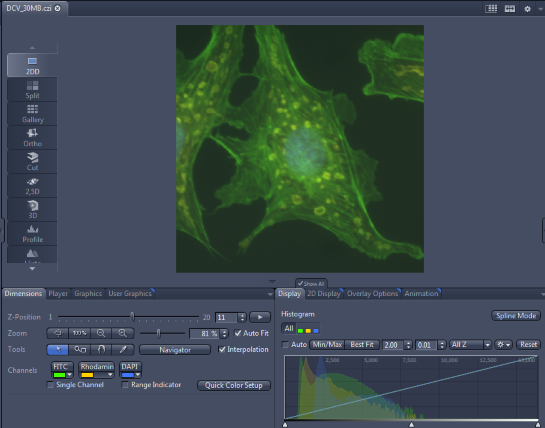
\includegraphics[width=\textwidth,height=\textheight/2,keepaspectratio=true]{ZEN_screenshot_2.PNG}
\doxyfigcaption{3-\/channel document in Z\+EN}
\end{DoxyImage}


The following arguments are meaningful for this command\+:
\begin{DoxyItemize}
\item \textquotesingle{}-\/p\textquotesingle{} or \textquotesingle{}-\/-\/plane-\/coordinate\textquotesingle{}
\item \textquotesingle{}-\/r\textquotesingle{} or \textquotesingle{}-\/-\/rect\textquotesingle{}
\item \textquotesingle{}-\/j\textquotesingle{} or \textquotesingle{}-\/-\/jpgxrcodec\textquotesingle{}
\item \textquotesingle{}-\/b\textquotesingle{} or \textquotesingle{}-\/-\/background\textquotesingle{}
\item \textquotesingle{}-\/d\textquotesingle{} or \textquotesingle{}-\/-\/display-\/settings\textquotesingle{}
\item \textquotesingle{}-\/f\textquotesingle{} or \textquotesingle{}-\/-\/tile-\/filter\textquotesingle{}
\end{DoxyItemize}

In order to specify the display-\/settings on the commandline, a J\+S\+O\+N-\/notation is used -\/ an example is shown here\+: \begin{DoxyVerb}{
  "channels": [
    {
      "ch": 0,
      "tinting": "#41ff00",
      "weight": 1,
      "black-point": 0,
      "white-point": 0.15259021896696423
    },
    {
      "ch": 1,
      "tinting": "#ffd200",
      "weight": 1,
      "black-point": 0,
      "white-point": 0.15259021896696423
    },
    {
      "ch": 2,
      "tinting": "#4178ff",
      "weight": 1,
      "black-point": 0,
      "white-point": 0.15259021896696423
    }
  ]
}
\end{DoxyVerb}


It is an array \char`\"{}channels\char`\"{}, where the following fields are possible\+:

\tabulinesep=1mm
\begin{longtabu} spread 0pt [c]{*{3}{|X[-1]}|}
\hline
\rowcolor{\tableheadbgcolor}\textbf{ field name }&\textbf{ type }&\textbf{ explanation  }\\\cline{1-3}
\endfirsthead
\hline
\endfoot
\hline
\rowcolor{\tableheadbgcolor}\textbf{ field name }&\textbf{ type }&\textbf{ explanation  }\\\cline{1-3}
\endhead
ch &integer &the channel-\/index for which this channel-\/display-\/settings applies to \\\cline{1-3}
black-\/point &number &the black-\/point (default\+: 0) \\\cline{1-3}
white-\/point &number &the white-\/point (default\+: 1) \\\cline{1-3}
tinting &string &gives the R\+G\+B24-\/color as a 6-\/digit hexadecimal number, must start with a hash (\textquotesingle{}\#\textquotesingle{}) \\\cline{1-3}
gamma &number &the gradation curve is defined by a gamma with the value given here \\\cline{1-3}
splinelut &array of numbers &the gradation curve is defined a spline, and the list of numbers are the x and y coordinates of the control-\/points of a spline \\\cline{1-3}
\end{longtabu}
Note that \textquotesingle{}gamma\textquotesingle{} and \textquotesingle{}splinelut\textquotesingle{} are mutually exclusive, if both happen to be present, then \textquotesingle{}gamma\textquotesingle{} takes precedence.

An example for a display-\/setting when specifying a spline is\+: \begin{DoxyVerb}{
  "channels": [
    {
      "ch": 0,
      "splinelut": [
        0.362559241706161,  0.876190476190476,
        0.554502369668246,  0.561904761904762
      ]
    }
  ]
}
\end{DoxyVerb}


Note that it is a flat list of numbers, where the first number is interpreted as X and the second as Y -\/ and so on.

Passing this J\+S\+ON on the commandline might be challenging, though -\/ because many characters need to be escaped (depending on your command shell).

\subsection*{command \textquotesingle{}Extract\+Attachment\textquotesingle{}}

The command \textquotesingle{}Extract\+Attachment\textquotesingle{} allows to extract attachments and save them to a distinct file. \begin{DoxyVerb}>CZIcmd.exe --command ExtractAttachment --source D:\PICTURES\NaCZIrTestData\Example_TMA1_Zeb1_SPRR2_Ck19_S100-1-1-1-1.czi --output attachments

>dir

 Volume in drive D is DATA
 Volume Serial Number is 74F9-A4A3

 Directory of D:\TFSJBL\LibCZIDistrib\Src\Build\VS\Win32\Release\out

05/11/2016  12:56 PM    <DIR>          .
05/11/2016  12:56 PM    <DIR>          ..
05/11/2016  12:56 PM               158 attachments_EventList_1.CZEVL
05/11/2016  12:56 PM         2,887,520 attachments_Label_2.CZI
05/11/2016  12:56 PM         6,744,768 attachments_SlidePreview_3.CZI
05/11/2016  12:56 PM             3,904 attachments_Thumbnail_4.JPG
05/11/2016  12:56 PM                16 attachments_TimeStamps_0.CZTIMS
               5 File(s)      9,636,366 bytes
               2 Dir(s)  519,149,056,000 bytes free
\end{DoxyVerb}


The filename of the attachments is composed from the -\/-\/output-\/argument, appending the name of the attachment and its id. The extension is given by the \textquotesingle{}filetype\textquotesingle{}-\/field of the attachment.

In the above example, all attachments are processed. It is possible to filter the attachments -\/ by giving the name or the index. This is specified with the -\/-\/selection-\/argument\+: \begin{DoxyVerb}>CZIcmd.exe --command ExtractAttachment --source D:\PICTURES\NaCZIrTestData\Example_TMA1_Zeb1_SPRR2_Ck19_S100-1-1-1-1.czi --output attachments --selection {\"name\":\"Thumbnail\"}
\end{DoxyVerb}


This will only save the attachments with \textquotesingle{}name\textquotesingle{} = \char`\"{}\+Thumbnail\char`\"{}. \begin{DoxyVerb}>CZIcmd.exe --command ExtractAttachment --source D:\PICTURES\NaCZIrTestData\Example_TMA1_Zeb1_SPRR2_Ck19_S100-1-1-1-1.czi --output attachments --selection {\"index\":1.0}
\end{DoxyVerb}


This will only save the attachments with id = 1. 
\chapter{3rd party software}
\label{_3rdpartysoftware}
\Hypertarget{_3rdpartysoftware}
In the lib\+C\+Z\+I-\/library and its sample-\/code the following 3rd-\/party-\/software is used\+:

\tabulinesep=1mm
\begin{longtabu} spread 0pt [c]{*{5}{|X[-1]}|}
\hline
\rowcolor{\tableheadbgcolor}\textbf{ name }&\textbf{ purpose }&\textbf{ license }&\textbf{ comment }&\textbf{ source included  }\\\cline{1-5}
\endfirsthead
\hline
\endfoot
\hline
\rowcolor{\tableheadbgcolor}\textbf{ name }&\textbf{ purpose }&\textbf{ license }&\textbf{ comment }&\textbf{ source included  }\\\cline{1-5}
\endhead
\href{https://github.com/zeux/pugixml}{\tt pugixml} &X\+M\+L-\/parser &\href{https://opensource.org/licenses/MIT}{\tt M\+IT} &&yes \\\cline{1-5}
\href{http://eigen.tuxfamily.org/}{\tt Eigen} &linear algebra &\href{https://opensource.org/licenses/MPL-2.0}{\tt M\+P\+L2} &used for very basic stuff &yes \\\cline{1-5}
\href{http://rapidjson.org/}{\tt Rapid\+J\+S\+ON} &J\+S\+ON parser/genertor &\href{https://opensource.org/licenses/MIT}{\tt M\+IT} &used in C\+Z\+Icmd &yes \\\cline{1-5}
\href{https://jxrlib.codeplex.com/}{\tt jxrlib} &J\+P\+G-\/\+XR codec &\href{https://opensource.org/licenses/BSD-2-Clause}{\tt B\+SD 2-\/\+Clause} &code has some modifictions &yes \\\cline{1-5}
\href{http://libpng.org/pub/png/libpng.html}{\tt libpng} &write P\+N\+Gs &\href{http://libpng.org/pub/png/src/libpng-LICENSE.txt}{\tt libpng license} &used in C\+Z\+I\+Cmd (on Linux) &no \\\cline{1-5}
\href{https://github.com/bluebaroncanada/getoptW}{\tt getoptW}&commandline args parser &\href{https://github.com/bluebaroncanada/getoptW/#licence]}{\tt get\+OptW license}&used in C\+Z\+I\+Cmd (on Windows) &yes \\\cline{1-5}
\href{https://sourceforge.net/projects/md5sum/}{\tt md5sum} &M\+D5\+Sum hash &\href{http://www.cv.nrao.edu/glish/copyright/md5.html}{\tt M\+D5\+Sum license} &&yes \\\cline{1-5}
\end{longtabu}

\chapter{Todos}
\label{todos}
\Hypertarget{todos}
Listing some features and ideas that did not make it into this version. This list is of course not exhaustive.

\tabulinesep=1mm
\begin{longtabu} spread 0pt [c]{*{2}{|X[-1]}|}
\hline
\rowcolor{\tableheadbgcolor}\textbf{ feature }&\textbf{ comment  }\\\cline{1-2}
\endfirsthead
\hline
\endfoot
\hline
\rowcolor{\tableheadbgcolor}\textbf{ feature }&\textbf{ comment  }\\\cline{1-2}
\endhead
support for Gray32\+Float &The pixeltype Gray32\+Float (in fact, all but Gray8, Gray16, Bgr24 and Bgr48) is not supported with Compose\+Multi\+Channel\+\_\+\+Bgr24.~\newline
Also, the simple conversion (with the Get-\/method of accessors) is not implemented for all pixeltypes. \\\cline{1-2}
support for \char`\"{}tinting L\+U\+Ts\char`\"{} &This feature of display-\/settings in Z\+EN is not yet implemented\+:~\newline

\begin{DoxyImage}
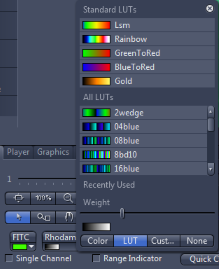
\includegraphics[width=7cm]{Tinting-LUT.png}
\doxyfigcaption{tinting lut in Z\+EN}
\end{DoxyImage}
 \\\cline{1-2}
domain objects for metadata &for accessing the metadata there is very little support (besides parsing the X\+ML by hand) \\\cline{1-2}
performance &Performance has not been a priority so far. Performance has many aspects, and as far as the library (and its anticipated use) is concerned, it is expected that the most important task is to provide caching.~\newline
Besides, in the composition the use of S\+I\+M\+D-\/code would surely be beneficial. \\\cline{1-2}
sub-\/block metadata &Currently no domain objects for sub-\/block metadata, only raw-\/\+X\+ML is accesible. \\\cline{1-2}
support for mask &Support for the \char`\"{}valid pixel mask\char`\"{}-\/feature is not implemented. \\\cline{1-2}
multi-\/channel-\/composition~\newline
for pixeltype Bgr48 &This would be a function akin to Compose\+Multi\+Channel\+\_\+\+Bgr24 ⇒ Compose\+Multi\+Channel\+\_\+\+Bgr48. \\\cline{1-2}
\end{longtabu}
Besides those features which are missing somewhat undisputed, there are of course a lot of ideas what could be added. Here are some ideas listed\+:

\tabulinesep=1mm
\begin{longtabu} spread 0pt [c]{*{2}{|X[-1]}|}
\hline
\rowcolor{\tableheadbgcolor}\textbf{ feature }&\textbf{ comment  }\\\cline{1-2}
\endfirsthead
\hline
\endfoot
\hline
\rowcolor{\tableheadbgcolor}\textbf{ feature }&\textbf{ comment  }\\\cline{1-2}
\endhead
bindings &Provide bindings and samples for popular languages and software (Java, Python, Mat\+Lab, Mathematica, ImageJ, Open\+CV, ...) \\\cline{1-2}
support for authoring C\+Z\+I-\/files&Writing C\+Z\+Is should not be harder than reading them \\\cline{1-2}
\end{longtabu}

\chapter{Namespace Index}
\section{Namespace List}
Here is a list of all documented namespaces with brief descriptions\+:\begin{DoxyCompactList}
\item\contentsline{section}{\hyperlink{namespacelib_c_z_i}{lib\+C\+ZI} \\*External interfaces, classes, functions and structs are found in the namespace \char`\"{}lib\+C\+Z\+I\char`\"{} }{\pageref{namespacelib_c_z_i}}{}
\end{DoxyCompactList}

\chapter{Hierarchical Index}
\section{Class Hierarchy}
This inheritance list is sorted roughly, but not completely, alphabetically\+:\begin{DoxyCompactList}
\item \contentsline{section}{lib\+C\+ZI\+:\+:Attachment\+Info}{\pageref{structlib_c_z_i_1_1_attachment_info}}{}
\item \contentsline{section}{lib\+C\+ZI\+:\+:Bitmap\+Lock\+Info}{\pageref{structlib_c_z_i_1_1_bitmap_lock_info}}{}
\begin{DoxyCompactList}
\item \contentsline{section}{lib\+C\+ZI\+:\+:Scoped\+Bitmap\+Locker$<$ t\+Bitmap $>$}{\pageref{classlib_c_z_i_1_1_scoped_bitmap_locker}}{}
\end{DoxyCompactList}
\item \contentsline{section}{lib\+C\+ZI\+:\+:Bounding\+Boxes}{\pageref{structlib_c_z_i_1_1_bounding_boxes}}{}
\item \contentsline{section}{lib\+C\+ZI\+:\+:Build\+Information}{\pageref{structlib_c_z_i_1_1_build_information}}{}
\item \contentsline{section}{lib\+C\+ZI\+:\+:C\+Dim\+Base}{\pageref{classlib_c_z_i_1_1_c_dim_base}}{}
\begin{DoxyCompactList}
\item \contentsline{section}{lib\+C\+ZI\+:\+:C\+Dim\+Bounds}{\pageref{classlib_c_z_i_1_1_c_dim_bounds}}{}
\item \contentsline{section}{lib\+C\+ZI\+:\+:C\+Dim\+Coordinate}{\pageref{classlib_c_z_i_1_1_c_dim_coordinate}}{}
\end{DoxyCompactList}
\item \contentsline{section}{lib\+C\+ZI\+:\+:Channel\+Display\+Settings\+P\+OD}{\pageref{structlib_c_z_i_1_1_channel_display_settings_p_o_d}}{}
\item \contentsline{section}{lib\+C\+ZI\+:\+:Compositors\+:\+:Channel\+Info}{\pageref{structlib_c_z_i_1_1_compositors_1_1_channel_info}}{}
\item \contentsline{section}{lib\+C\+ZI\+:\+:Compositors\+:\+:Compose\+Single\+Tile\+Options}{\pageref{structlib_c_z_i_1_1_compositors_1_1_compose_single_tile_options}}{}
\item \contentsline{section}{lib\+C\+ZI\+:\+:Compositors}{\pageref{classlib_c_z_i_1_1_compositors}}{}
\item \contentsline{section}{lib\+C\+ZI\+:\+:I\+Display\+Settings\+:\+:Cubic\+Spline\+Coefficients}{\pageref{structlib_c_z_i_1_1_i_display_settings_1_1_cubic_spline_coefficients}}{}
\item \contentsline{section}{lib\+C\+ZI\+:\+:Dbl\+Rect}{\pageref{structlib_c_z_i_1_1_dbl_rect}}{}
\item \contentsline{section}{lib\+C\+ZI\+:\+:Dimension\+And\+Start\+Size}{\pageref{structlib_c_z_i_1_1_dimension_and_start_size}}{}
\item \contentsline{section}{lib\+C\+ZI\+:\+:Dimension\+And\+Value}{\pageref{structlib_c_z_i_1_1_dimension_and_value}}{}
\item \contentsline{section}{lib\+C\+ZI\+:\+:Display\+Settings\+P\+OD}{\pageref{structlib_c_z_i_1_1_display_settings_p_o_d}}{}
\item \contentsline{section}{lib\+C\+ZI\+:\+:File\+Header\+Info}{\pageref{structlib_c_z_i_1_1_file_header_info}}{}
\item \contentsline{section}{lib\+C\+ZI\+:\+:General\+Document\+Info}{\pageref{structlib_c_z_i_1_1_general_document_info}}{}
\item \contentsline{section}{lib\+C\+ZI\+:\+:I\+Accessor}{\pageref{classlib_c_z_i_1_1_i_accessor}}{}
\begin{DoxyCompactList}
\item \contentsline{section}{lib\+C\+ZI\+:\+:I\+Single\+Channel\+Pyramid\+Layer\+Tile\+Accessor}{\pageref{classlib_c_z_i_1_1_i_single_channel_pyramid_layer_tile_accessor}}{}
\item \contentsline{section}{lib\+C\+ZI\+:\+:I\+Single\+Channel\+Scaling\+Tile\+Accessor}{\pageref{classlib_c_z_i_1_1_i_single_channel_scaling_tile_accessor}}{}
\item \contentsline{section}{lib\+C\+ZI\+:\+:I\+Single\+Channel\+Tile\+Accessor}{\pageref{classlib_c_z_i_1_1_i_single_channel_tile_accessor}}{}
\end{DoxyCompactList}
\item \contentsline{section}{lib\+C\+ZI\+:\+:I\+Attachment}{\pageref{classlib_c_z_i_1_1_i_attachment}}{}
\item \contentsline{section}{lib\+C\+ZI\+:\+:I\+Attachment\+Repository}{\pageref{classlib_c_z_i_1_1_i_attachment_repository}}{}
\begin{DoxyCompactList}
\item \contentsline{section}{lib\+C\+ZI\+:\+:I\+C\+Z\+I\+Reader}{\pageref{classlib_c_z_i_1_1_i_c_z_i_reader}}{}
\end{DoxyCompactList}
\item \contentsline{section}{lib\+C\+ZI\+:\+:I\+Bitmap\+Data}{\pageref{classlib_c_z_i_1_1_i_bitmap_data}}{}
\item \contentsline{section}{lib\+C\+ZI\+:\+:I\+Channel\+Display\+Setting}{\pageref{classlib_c_z_i_1_1_i_channel_display_setting}}{}
\item \contentsline{section}{lib\+C\+ZI\+:\+:I\+Czi\+Multi\+Dimension\+Document\+Info}{\pageref{classlib_c_z_i_1_1_i_czi_multi_dimension_document_info}}{}
\item \contentsline{section}{lib\+C\+ZI\+:\+:I\+Decoder}{\pageref{classlib_c_z_i_1_1_i_decoder}}{}
\item \contentsline{section}{lib\+C\+ZI\+:\+:I\+Dim\+Bounds}{\pageref{classlib_c_z_i_1_1_i_dim_bounds}}{}
\begin{DoxyCompactList}
\item \contentsline{section}{lib\+C\+ZI\+:\+:C\+Dim\+Bounds}{\pageref{classlib_c_z_i_1_1_c_dim_bounds}}{}
\end{DoxyCompactList}
\item \contentsline{section}{lib\+C\+ZI\+:\+:I\+Dim\+Coordinate}{\pageref{classlib_c_z_i_1_1_i_dim_coordinate}}{}
\begin{DoxyCompactList}
\item \contentsline{section}{lib\+C\+ZI\+:\+:C\+Dim\+Coordinate}{\pageref{classlib_c_z_i_1_1_c_dim_coordinate}}{}
\end{DoxyCompactList}
\item \contentsline{section}{lib\+C\+ZI\+:\+:I\+Dimension\+Info}{\pageref{classlib_c_z_i_1_1_i_dimension_info}}{}
\item \contentsline{section}{lib\+C\+ZI\+:\+:I\+Dimension\+T\+Info}{\pageref{classlib_c_z_i_1_1_i_dimension_t_info}}{}
\item \contentsline{section}{lib\+C\+ZI\+:\+:I\+Dimension\+Z\+Info}{\pageref{classlib_c_z_i_1_1_i_dimension_z_info}}{}
\item \contentsline{section}{lib\+C\+ZI\+:\+:I\+Display\+Settings}{\pageref{classlib_c_z_i_1_1_i_display_settings}}{}
\item \contentsline{section}{lib\+C\+ZI\+:\+:I\+Index\+Set}{\pageref{classlib_c_z_i_1_1_i_index_set}}{}
\item \contentsline{section}{lib\+C\+ZI\+:\+:I\+Metadata\+Segment}{\pageref{classlib_c_z_i_1_1_i_metadata_segment}}{}
\item \contentsline{section}{lib\+C\+ZI\+:\+:Int\+Rect}{\pageref{structlib_c_z_i_1_1_int_rect}}{}
\item \contentsline{section}{lib\+C\+ZI\+:\+:Int\+Size}{\pageref{structlib_c_z_i_1_1_int_size}}{}
\item \contentsline{section}{lib\+C\+ZI\+:\+:I\+Site}{\pageref{classlib_c_z_i_1_1_i_site}}{}
\item \contentsline{section}{lib\+C\+ZI\+:\+:I\+Stream}{\pageref{classlib_c_z_i_1_1_i_stream}}{}
\item \contentsline{section}{lib\+C\+ZI\+:\+:I\+Sub\+Block}{\pageref{classlib_c_z_i_1_1_i_sub_block}}{}
\item \contentsline{section}{lib\+C\+ZI\+:\+:I\+Sub\+Block\+Repository}{\pageref{classlib_c_z_i_1_1_i_sub_block_repository}}{}
\begin{DoxyCompactList}
\item \contentsline{section}{lib\+C\+ZI\+:\+:I\+C\+Z\+I\+Reader}{\pageref{classlib_c_z_i_1_1_i_c_z_i_reader}}{}
\end{DoxyCompactList}
\item \contentsline{section}{lib\+C\+ZI\+:\+:I\+Xml\+Node\+Read}{\pageref{classlib_c_z_i_1_1_i_xml_node_read}}{}
\begin{DoxyCompactList}
\item \contentsline{section}{lib\+C\+ZI\+:\+:I\+Czi\+Metadata}{\pageref{classlib_c_z_i_1_1_i_czi_metadata}}{}
\end{DoxyCompactList}
\item nested\+\_\+exception\begin{DoxyCompactList}
\item \contentsline{section}{lib\+C\+ZI\+:\+:Lib\+C\+Z\+I\+I\+O\+Exception}{\pageref{classlib_c_z_i_1_1_lib_c_z_i_i_o_exception}}{}
\end{DoxyCompactList}
\item \contentsline{section}{lib\+C\+ZI\+:\+:I\+Single\+Channel\+Scaling\+Tile\+Accessor\+:\+:Options}{\pageref{structlib_c_z_i_1_1_i_single_channel_scaling_tile_accessor_1_1_options}}{}
\item \contentsline{section}{lib\+C\+ZI\+:\+:I\+Single\+Channel\+Tile\+Accessor\+:\+:Options}{\pageref{structlib_c_z_i_1_1_i_single_channel_tile_accessor_1_1_options}}{}
\item \contentsline{section}{lib\+C\+ZI\+:\+:I\+Single\+Channel\+Pyramid\+Layer\+Tile\+Accessor\+:\+:Options}{\pageref{structlib_c_z_i_1_1_i_single_channel_pyramid_layer_tile_accessor_1_1_options}}{}
\item \contentsline{section}{lib\+C\+ZI\+:\+:I\+Single\+Channel\+Pyramid\+Layer\+Tile\+Accessor\+:\+:Pyramid\+Layer\+Info}{\pageref{structlib_c_z_i_1_1_i_single_channel_pyramid_layer_tile_accessor_1_1_pyramid_layer_info}}{}
\item \contentsline{section}{lib\+C\+ZI\+:\+:Pyramid\+Statistics\+:\+:Pyramid\+Layer\+Info}{\pageref{structlib_c_z_i_1_1_pyramid_statistics_1_1_pyramid_layer_info}}{}
\item \contentsline{section}{lib\+C\+ZI\+:\+:Pyramid\+Statistics\+:\+:Pyramid\+Layer\+Statistics}{\pageref{structlib_c_z_i_1_1_pyramid_statistics_1_1_pyramid_layer_statistics}}{}
\item \contentsline{section}{lib\+C\+ZI\+:\+:Pyramid\+Statistics}{\pageref{structlib_c_z_i_1_1_pyramid_statistics}}{}
\item \contentsline{section}{lib\+C\+ZI\+:\+:Rgb8\+Color}{\pageref{structlib_c_z_i_1_1_rgb8_color}}{}
\item \contentsline{section}{lib\+C\+ZI\+:\+:Rgb\+Float\+Color}{\pageref{structlib_c_z_i_1_1_rgb_float_color}}{}
\item runtime\+\_\+error\begin{DoxyCompactList}
\item \contentsline{section}{lib\+C\+ZI\+:\+:Lib\+C\+Z\+I\+Exception}{\pageref{classlib_c_z_i_1_1_lib_c_z_i_exception}}{}
\begin{DoxyCompactList}
\item \contentsline{section}{lib\+C\+ZI\+:\+:Lib\+C\+Z\+I\+Accessor\+Exception}{\pageref{classlib_c_z_i_1_1_lib_c_z_i_accessor_exception}}{}
\item \contentsline{section}{lib\+C\+ZI\+:\+:Lib\+C\+Z\+I\+C\+Z\+I\+Parse\+Exception}{\pageref{structlib_c_z_i_1_1_lib_c_z_i_c_z_i_parse_exception}}{}
\item \contentsline{section}{lib\+C\+ZI\+:\+:Lib\+C\+Z\+I\+Invalid\+Plane\+Coordinate\+Exception}{\pageref{structlib_c_z_i_1_1_lib_c_z_i_invalid_plane_coordinate_exception}}{}
\item \contentsline{section}{lib\+C\+ZI\+:\+:Lib\+C\+Z\+I\+I\+O\+Exception}{\pageref{classlib_c_z_i_1_1_lib_c_z_i_i_o_exception}}{}
\item \contentsline{section}{lib\+C\+ZI\+:\+:Lib\+C\+Z\+I\+Metadata\+Exception}{\pageref{classlib_c_z_i_1_1_lib_c_z_i_metadata_exception}}{}
\item \contentsline{section}{lib\+C\+ZI\+:\+:Lib\+C\+Z\+I\+Query\+Execution\+Exception}{\pageref{classlib_c_z_i_1_1_lib_c_z_i_query_execution_exception}}{}
\item \contentsline{section}{lib\+C\+ZI\+:\+:Lib\+C\+Z\+I\+Query\+Parse\+Exception}{\pageref{classlib_c_z_i_1_1_lib_c_z_i_query_parse_exception}}{}
\item \contentsline{section}{lib\+C\+ZI\+:\+:Lib\+C\+Z\+I\+String\+Parse\+Exception}{\pageref{classlib_c_z_i_1_1_lib_c_z_i_string_parse_exception}}{}
\item \contentsline{section}{lib\+C\+ZI\+:\+:Lib\+C\+Z\+I\+Xml\+Parse\+Exception}{\pageref{classlib_c_z_i_1_1_lib_c_z_i_xml_parse_exception}}{}
\end{DoxyCompactList}
\end{DoxyCompactList}
\item \contentsline{section}{lib\+C\+ZI\+:\+:Scaling\+Info}{\pageref{structlib_c_z_i_1_1_scaling_info}}{}
\begin{DoxyCompactList}
\item \contentsline{section}{lib\+C\+ZI\+:\+:Scaling\+Info\+Ex}{\pageref{structlib_c_z_i_1_1_scaling_info_ex}}{}
\end{DoxyCompactList}
\item \contentsline{section}{lib\+C\+ZI\+:\+:I\+Display\+Settings\+:\+:Spline\+Control\+Point}{\pageref{structlib_c_z_i_1_1_i_display_settings_1_1_spline_control_point}}{}
\item \contentsline{section}{lib\+C\+ZI\+:\+:I\+Display\+Settings\+:\+:Spline\+Data}{\pageref{structlib_c_z_i_1_1_i_display_settings_1_1_spline_data}}{}
\item \contentsline{section}{lib\+C\+ZI\+:\+:Sub\+Block\+Info}{\pageref{structlib_c_z_i_1_1_sub_block_info}}{}
\item \contentsline{section}{lib\+C\+ZI\+:\+:Sub\+Block\+Statistics}{\pageref{structlib_c_z_i_1_1_sub_block_statistics}}{}
\item \contentsline{section}{lib\+C\+ZI\+:\+:Compositors\+:\+:Tinting\+Color}{\pageref{structlib_c_z_i_1_1_compositors_1_1_tinting_color}}{}
\item \contentsline{section}{lib\+C\+ZI\+:\+:Utils}{\pageref{classlib_c_z_i_1_1_utils}}{}
\item \contentsline{section}{lib\+C\+ZI\+:\+:Xml\+Date\+Time}{\pageref{structlib_c_z_i_1_1_xml_date_time}}{}
\end{DoxyCompactList}

\chapter{Class Index}
\section{Class List}
Here are the classes, structs, unions and interfaces with brief descriptions\+:\begin{DoxyCompactList}
\item\contentsline{section}{\hyperlink{structlib_c_z_i_1_1_attachment_info}{lib\+C\+Z\+I\+::\+Attachment\+Info} \\*Information about an attachment }{\pageref{structlib_c_z_i_1_1_attachment_info}}{}
\item\contentsline{section}{\hyperlink{structlib_c_z_i_1_1_bitmap_lock_info}{lib\+C\+Z\+I\+::\+Bitmap\+Lock\+Info} \\*Information about a locked bitmap -\/ allowing direct access to the image data in memory }{\pageref{structlib_c_z_i_1_1_bitmap_lock_info}}{}
\item\contentsline{section}{\hyperlink{structlib_c_z_i_1_1_bounding_boxes}{lib\+C\+Z\+I\+::\+Bounding\+Boxes} \\*This structure gathers the bounding-\/boxes determined from all sub-\/blocks and only be those on pyramid-\/layer 0 }{\pageref{structlib_c_z_i_1_1_bounding_boxes}}{}
\item\contentsline{section}{\hyperlink{structlib_c_z_i_1_1_build_information}{lib\+C\+Z\+I\+::\+Build\+Information} }{\pageref{structlib_c_z_i_1_1_build_information}}{}
\item\contentsline{section}{\hyperlink{classlib_c_z_i_1_1_c_dim_base}{lib\+C\+Z\+I\+::\+C\+Dim\+Base} \\*Base class containing some commonly used methods }{\pageref{classlib_c_z_i_1_1_c_dim_base}}{}
\item\contentsline{section}{\hyperlink{classlib_c_z_i_1_1_c_dim_bounds}{lib\+C\+Z\+I\+::\+C\+Dim\+Bounds} \\*Implementation of a class representing an interval (and implementing the {\ttfamily \hyperlink{classlib_c_z_i_1_1_i_dim_bounds}{lib\+C\+Z\+I\+::\+I\+Dim\+Bounds}}-\/interface) }{\pageref{classlib_c_z_i_1_1_c_dim_bounds}}{}
\item\contentsline{section}{\hyperlink{classlib_c_z_i_1_1_c_dim_coordinate}{lib\+C\+Z\+I\+::\+C\+Dim\+Coordinate} \\*Implementation of a class representing a coordinate (and implementing the {\ttfamily \hyperlink{classlib_c_z_i_1_1_i_dim_coordinate}{I\+Dim\+Coordinate}}-\/interface) }{\pageref{classlib_c_z_i_1_1_c_dim_coordinate}}{}
\item\contentsline{section}{\hyperlink{structlib_c_z_i_1_1_channel_display_settings_p_o_d}{lib\+C\+Z\+I\+::\+Channel\+Display\+Settings\+P\+OD} }{\pageref{structlib_c_z_i_1_1_channel_display_settings_p_o_d}}{}
\item\contentsline{section}{\hyperlink{structlib_c_z_i_1_1_compositors_1_1_channel_info}{lib\+C\+Z\+I\+::\+Compositors\+::\+Channel\+Info} }{\pageref{structlib_c_z_i_1_1_compositors_1_1_channel_info}}{}
\item\contentsline{section}{\hyperlink{structlib_c_z_i_1_1_compositors_1_1_compose_single_tile_options}{lib\+C\+Z\+I\+::\+Compositors\+::\+Compose\+Single\+Tile\+Options} \\*Options for the \hyperlink{classlib_c_z_i_1_1_compositors_a8b39ab77c8b83a5a5a8a7e1773e8ad7a}{lib\+C\+Z\+I\+::\+Compositors\+::\+Compose\+Single\+Channel\+Tiles} function }{\pageref{structlib_c_z_i_1_1_compositors_1_1_compose_single_tile_options}}{}
\item\contentsline{section}{\hyperlink{classlib_c_z_i_1_1_compositors}{lib\+C\+Z\+I\+::\+Compositors} \\*Composition operations are found in this class\+: multi-\/tile compositor and multi-\/channel compositor }{\pageref{classlib_c_z_i_1_1_compositors}}{}
\item\contentsline{section}{\hyperlink{structlib_c_z_i_1_1_i_display_settings_1_1_cubic_spline_coefficients}{lib\+C\+Z\+I\+::\+I\+Display\+Settings\+::\+Cubic\+Spline\+Coefficients} \\*The coefficients of a cubic spline defined by $a\,x^3 + b\,x^2 + c\,x + d =y$ }{\pageref{structlib_c_z_i_1_1_i_display_settings_1_1_cubic_spline_coefficients}}{}
\item\contentsline{section}{\hyperlink{structlib_c_z_i_1_1_dbl_rect}{lib\+C\+Z\+I\+::\+Dbl\+Rect} \\*A rectangle (with double coordinates) }{\pageref{structlib_c_z_i_1_1_dbl_rect}}{}
\item\contentsline{section}{\hyperlink{structlib_c_z_i_1_1_dimension_and_start_size}{lib\+C\+Z\+I\+::\+Dimension\+And\+Start\+Size} \\*A structure combining a dimension and an interval (defined by a start value and the size) }{\pageref{structlib_c_z_i_1_1_dimension_and_start_size}}{}
\item\contentsline{section}{\hyperlink{structlib_c_z_i_1_1_dimension_and_value}{lib\+C\+Z\+I\+::\+Dimension\+And\+Value} \\*A structure combining a dimension and a value }{\pageref{structlib_c_z_i_1_1_dimension_and_value}}{}
\item\contentsline{section}{\hyperlink{structlib_c_z_i_1_1_display_settings_p_o_d}{lib\+C\+Z\+I\+::\+Display\+Settings\+P\+OD} }{\pageref{structlib_c_z_i_1_1_display_settings_p_o_d}}{}
\item\contentsline{section}{\hyperlink{structlib_c_z_i_1_1_file_header_info}{lib\+C\+Z\+I\+::\+File\+Header\+Info} \\*Global information about the C\+Z\+I-\/file (from the C\+Z\+I-\/fileheader-\/segment) }{\pageref{structlib_c_z_i_1_1_file_header_info}}{}
\item\contentsline{section}{\hyperlink{structlib_c_z_i_1_1_general_document_info}{lib\+C\+Z\+I\+::\+General\+Document\+Info} \\*General document information -\/ corresponding to Information/\+Document }{\pageref{structlib_c_z_i_1_1_general_document_info}}{}
\item\contentsline{section}{\hyperlink{classlib_c_z_i_1_1_i_accessor}{lib\+C\+Z\+I\+::\+I\+Accessor} \\*The base interface (all accessor-\/interface must derive from this) }{\pageref{classlib_c_z_i_1_1_i_accessor}}{}
\item\contentsline{section}{\hyperlink{classlib_c_z_i_1_1_i_attachment}{lib\+C\+Z\+I\+::\+I\+Attachment} \\*Representation of an attachment. An attachment is a binary blob, its inner structure is opaque }{\pageref{classlib_c_z_i_1_1_i_attachment}}{}
\item\contentsline{section}{\hyperlink{classlib_c_z_i_1_1_i_attachment_repository}{lib\+C\+Z\+I\+::\+I\+Attachment\+Repository} \\*Interface for the attachment repository. This interface is used to access the attachments in a C\+Z\+I-\/file }{\pageref{classlib_c_z_i_1_1_i_attachment_repository}}{}
\item\contentsline{section}{\hyperlink{classlib_c_z_i_1_1_i_bitmap_data}{lib\+C\+Z\+I\+::\+I\+Bitmap\+Data} }{\pageref{classlib_c_z_i_1_1_i_bitmap_data}}{}
\item\contentsline{section}{\hyperlink{classlib_c_z_i_1_1_i_channel_display_setting}{lib\+C\+Z\+I\+::\+I\+Channel\+Display\+Setting} \\*The display-\/settings for a channel }{\pageref{classlib_c_z_i_1_1_i_channel_display_setting}}{}
\item\contentsline{section}{\hyperlink{classlib_c_z_i_1_1_i_czi_metadata}{lib\+C\+Z\+I\+::\+I\+Czi\+Metadata} \\*Representation of the C\+Z\+I-\/metadata }{\pageref{classlib_c_z_i_1_1_i_czi_metadata}}{}
\item\contentsline{section}{\hyperlink{classlib_c_z_i_1_1_i_czi_multi_dimension_document_info}{lib\+C\+Z\+I\+::\+I\+Czi\+Multi\+Dimension\+Document\+Info} \\*The top-\/level interface for the C\+Z\+I-\/metadata object }{\pageref{classlib_c_z_i_1_1_i_czi_multi_dimension_document_info}}{}
\item\contentsline{section}{\hyperlink{classlib_c_z_i_1_1_i_c_z_i_reader}{lib\+C\+Z\+I\+::\+I\+C\+Z\+I\+Reader} \\*This interface is used to represent the C\+Z\+I-\/file }{\pageref{classlib_c_z_i_1_1_i_c_z_i_reader}}{}
\item\contentsline{section}{\hyperlink{classlib_c_z_i_1_1_i_decoder}{lib\+C\+Z\+I\+::\+I\+Decoder} \\*The interface used for operating image decoder. That is the simplest possible interface at this point.. }{\pageref{classlib_c_z_i_1_1_i_decoder}}{}
\item\contentsline{section}{\hyperlink{classlib_c_z_i_1_1_i_dim_bounds}{lib\+C\+Z\+I\+::\+I\+Dim\+Bounds} \\*Interface used to represent an interval (for several dimensions) }{\pageref{classlib_c_z_i_1_1_i_dim_bounds}}{}
\item\contentsline{section}{\hyperlink{classlib_c_z_i_1_1_i_dim_coordinate}{lib\+C\+Z\+I\+::\+I\+Dim\+Coordinate} \\*Interface used to represent a coordinate (in the space of the dimensions identified by {\ttfamily Dimension\+Index}) }{\pageref{classlib_c_z_i_1_1_i_dim_coordinate}}{}
\item\contentsline{section}{\hyperlink{classlib_c_z_i_1_1_i_dimension_info}{lib\+C\+Z\+I\+::\+I\+Dimension\+Info} \\*Base class for information about the dimension }{\pageref{classlib_c_z_i_1_1_i_dimension_info}}{}
\item\contentsline{section}{\hyperlink{classlib_c_z_i_1_1_i_dimension_t_info}{lib\+C\+Z\+I\+::\+I\+Dimension\+T\+Info} \\*This structure defines the information for the \char`\"{}\+T-\/dimension\char`\"{}. It resembles the Z\+E\+N-\/metadata-\/structure \char`\"{}\+Dimensions/\+T\char`\"{} }{\pageref{classlib_c_z_i_1_1_i_dimension_t_info}}{}
\item\contentsline{section}{\hyperlink{classlib_c_z_i_1_1_i_dimension_z_info}{lib\+C\+Z\+I\+::\+I\+Dimension\+Z\+Info} \\*This structure defines the information for the \char`\"{}\+Z-\/dimension\char`\"{}. It resembles the Z\+E\+N-\/metadata-\/structure \char`\"{}\+Dimensions/\+Z\char`\"{} }{\pageref{classlib_c_z_i_1_1_i_dimension_z_info}}{}
\item\contentsline{section}{\hyperlink{classlib_c_z_i_1_1_i_display_settings}{lib\+C\+Z\+I\+::\+I\+Display\+Settings} \\*The display settings }{\pageref{classlib_c_z_i_1_1_i_display_settings}}{}
\item\contentsline{section}{\hyperlink{classlib_c_z_i_1_1_i_index_set}{lib\+C\+Z\+I\+::\+I\+Index\+Set} }{\pageref{classlib_c_z_i_1_1_i_index_set}}{}
\item\contentsline{section}{\hyperlink{classlib_c_z_i_1_1_i_metadata_segment}{lib\+C\+Z\+I\+::\+I\+Metadata\+Segment} \\*Interface representing the metadata-\/segment }{\pageref{classlib_c_z_i_1_1_i_metadata_segment}}{}
\item\contentsline{section}{\hyperlink{structlib_c_z_i_1_1_int_rect}{lib\+C\+Z\+I\+::\+Int\+Rect} \\*A rectangle (with integer coordinates) }{\pageref{structlib_c_z_i_1_1_int_rect}}{}
\item\contentsline{section}{\hyperlink{structlib_c_z_i_1_1_int_size}{lib\+C\+Z\+I\+::\+Int\+Size} \\*A structure representing a size (width and height) in integers }{\pageref{structlib_c_z_i_1_1_int_size}}{}
\item\contentsline{section}{\hyperlink{classlib_c_z_i_1_1_i_single_channel_pyramid_layer_tile_accessor}{lib\+C\+Z\+I\+::\+I\+Single\+Channel\+Pyramid\+Layer\+Tile\+Accessor} }{\pageref{classlib_c_z_i_1_1_i_single_channel_pyramid_layer_tile_accessor}}{}
\item\contentsline{section}{\hyperlink{classlib_c_z_i_1_1_i_single_channel_scaling_tile_accessor}{lib\+C\+Z\+I\+::\+I\+Single\+Channel\+Scaling\+Tile\+Accessor} }{\pageref{classlib_c_z_i_1_1_i_single_channel_scaling_tile_accessor}}{}
\item\contentsline{section}{\hyperlink{classlib_c_z_i_1_1_i_single_channel_tile_accessor}{lib\+C\+Z\+I\+::\+I\+Single\+Channel\+Tile\+Accessor} }{\pageref{classlib_c_z_i_1_1_i_single_channel_tile_accessor}}{}
\item\contentsline{section}{\hyperlink{classlib_c_z_i_1_1_i_site}{lib\+C\+Z\+I\+::\+I\+Site} }{\pageref{classlib_c_z_i_1_1_i_site}}{}
\item\contentsline{section}{\hyperlink{classlib_c_z_i_1_1_i_stream}{lib\+C\+Z\+I\+::\+I\+Stream} }{\pageref{classlib_c_z_i_1_1_i_stream}}{}
\item\contentsline{section}{\hyperlink{classlib_c_z_i_1_1_i_sub_block}{lib\+C\+Z\+I\+::\+I\+Sub\+Block} }{\pageref{classlib_c_z_i_1_1_i_sub_block}}{}
\item\contentsline{section}{\hyperlink{classlib_c_z_i_1_1_i_sub_block_repository}{lib\+C\+Z\+I\+::\+I\+Sub\+Block\+Repository} \\*Interface for sub-\/block repository. This interface is used to access the sub-\/blocks in a C\+Z\+I-\/file }{\pageref{classlib_c_z_i_1_1_i_sub_block_repository}}{}
\item\contentsline{section}{\hyperlink{classlib_c_z_i_1_1_i_xml_node_read}{lib\+C\+Z\+I\+::\+I\+Xml\+Node\+Read} \\*This interface provides read-\/only access to an X\+M\+L-\/node }{\pageref{classlib_c_z_i_1_1_i_xml_node_read}}{}
\item\contentsline{section}{\hyperlink{classlib_c_z_i_1_1_lib_c_z_i_accessor_exception}{lib\+C\+Z\+I\+::\+Lib\+C\+Z\+I\+Accessor\+Exception} \\*Exception for signaling errors specific for accessors }{\pageref{classlib_c_z_i_1_1_lib_c_z_i_accessor_exception}}{}
\item\contentsline{section}{\hyperlink{structlib_c_z_i_1_1_lib_c_z_i_c_z_i_parse_exception}{lib\+C\+Z\+I\+::\+Lib\+C\+Z\+I\+C\+Z\+I\+Parse\+Exception} \\*Exception for signaling errors parsing the C\+Z\+I-\/stream }{\pageref{structlib_c_z_i_1_1_lib_c_z_i_c_z_i_parse_exception}}{}
\item\contentsline{section}{\hyperlink{classlib_c_z_i_1_1_lib_c_z_i_exception}{lib\+C\+Z\+I\+::\+Lib\+C\+Z\+I\+Exception} \\*Base class for all lib\+C\+Z\+I-\/specific exceptions }{\pageref{classlib_c_z_i_1_1_lib_c_z_i_exception}}{}
\item\contentsline{section}{\hyperlink{structlib_c_z_i_1_1_lib_c_z_i_invalid_plane_coordinate_exception}{lib\+C\+Z\+I\+::\+Lib\+C\+Z\+I\+Invalid\+Plane\+Coordinate\+Exception} \\*Exception for signaling an incorrect plane-\/coordinate object }{\pageref{structlib_c_z_i_1_1_lib_c_z_i_invalid_plane_coordinate_exception}}{}
\item\contentsline{section}{\hyperlink{classlib_c_z_i_1_1_lib_c_z_i_i_o_exception}{lib\+C\+Z\+I\+::\+Lib\+C\+Z\+I\+I\+O\+Exception} }{\pageref{classlib_c_z_i_1_1_lib_c_z_i_i_o_exception}}{}
\item\contentsline{section}{\hyperlink{classlib_c_z_i_1_1_lib_c_z_i_metadata_exception}{lib\+C\+Z\+I\+::\+Lib\+C\+Z\+I\+Metadata\+Exception} \\*Exception for signaling errors when accessing the X\+M\+L-\/metadata }{\pageref{classlib_c_z_i_1_1_lib_c_z_i_metadata_exception}}{}
\item\contentsline{section}{\hyperlink{classlib_c_z_i_1_1_lib_c_z_i_query_execution_exception}{lib\+C\+Z\+I\+::\+Lib\+C\+Z\+I\+Query\+Execution\+Exception} \\*Exception for signaling errors when evaluating a query }{\pageref{classlib_c_z_i_1_1_lib_c_z_i_query_execution_exception}}{}
\item\contentsline{section}{\hyperlink{classlib_c_z_i_1_1_lib_c_z_i_query_parse_exception}{lib\+C\+Z\+I\+::\+Lib\+C\+Z\+I\+Query\+Parse\+Exception} \\*Exception for signaling errors when parsing a query-\/string }{\pageref{classlib_c_z_i_1_1_lib_c_z_i_query_parse_exception}}{}
\item\contentsline{section}{\hyperlink{classlib_c_z_i_1_1_lib_c_z_i_string_parse_exception}{lib\+C\+Z\+I\+::\+Lib\+C\+Z\+I\+String\+Parse\+Exception} \\*Exception for signaling that a string did not parse correctly }{\pageref{classlib_c_z_i_1_1_lib_c_z_i_string_parse_exception}}{}
\item\contentsline{section}{\hyperlink{classlib_c_z_i_1_1_lib_c_z_i_xml_parse_exception}{lib\+C\+Z\+I\+::\+Lib\+C\+Z\+I\+Xml\+Parse\+Exception} \\*Exception for signaling errors when parsing the X\+M\+L-\/metadata }{\pageref{classlib_c_z_i_1_1_lib_c_z_i_xml_parse_exception}}{}
\item\contentsline{section}{\hyperlink{structlib_c_z_i_1_1_i_single_channel_scaling_tile_accessor_1_1_options}{lib\+C\+Z\+I\+::\+I\+Single\+Channel\+Scaling\+Tile\+Accessor\+::\+Options} \\*\hyperlink{structlib_c_z_i_1_1_i_single_channel_scaling_tile_accessor_1_1_options}{Options} used for this accessor }{\pageref{structlib_c_z_i_1_1_i_single_channel_scaling_tile_accessor_1_1_options}}{}
\item\contentsline{section}{\hyperlink{structlib_c_z_i_1_1_i_single_channel_tile_accessor_1_1_options}{lib\+C\+Z\+I\+::\+I\+Single\+Channel\+Tile\+Accessor\+::\+Options} \\*\hyperlink{structlib_c_z_i_1_1_i_single_channel_tile_accessor_1_1_options}{Options} for controlling the composition operation }{\pageref{structlib_c_z_i_1_1_i_single_channel_tile_accessor_1_1_options}}{}
\item\contentsline{section}{\hyperlink{structlib_c_z_i_1_1_i_single_channel_pyramid_layer_tile_accessor_1_1_options}{lib\+C\+Z\+I\+::\+I\+Single\+Channel\+Pyramid\+Layer\+Tile\+Accessor\+::\+Options} \\*\hyperlink{structlib_c_z_i_1_1_i_single_channel_pyramid_layer_tile_accessor_1_1_options}{Options} used for this accessor }{\pageref{structlib_c_z_i_1_1_i_single_channel_pyramid_layer_tile_accessor_1_1_options}}{}
\item\contentsline{section}{\hyperlink{structlib_c_z_i_1_1_i_single_channel_pyramid_layer_tile_accessor_1_1_pyramid_layer_info}{lib\+C\+Z\+I\+::\+I\+Single\+Channel\+Pyramid\+Layer\+Tile\+Accessor\+::\+Pyramid\+Layer\+Info} }{\pageref{structlib_c_z_i_1_1_i_single_channel_pyramid_layer_tile_accessor_1_1_pyramid_layer_info}}{}
\item\contentsline{section}{\hyperlink{structlib_c_z_i_1_1_pyramid_statistics_1_1_pyramid_layer_info}{lib\+C\+Z\+I\+::\+Pyramid\+Statistics\+::\+Pyramid\+Layer\+Info} }{\pageref{structlib_c_z_i_1_1_pyramid_statistics_1_1_pyramid_layer_info}}{}
\item\contentsline{section}{\hyperlink{structlib_c_z_i_1_1_pyramid_statistics_1_1_pyramid_layer_statistics}{lib\+C\+Z\+I\+::\+Pyramid\+Statistics\+::\+Pyramid\+Layer\+Statistics} \\*Information about a pyramid-\/layer }{\pageref{structlib_c_z_i_1_1_pyramid_statistics_1_1_pyramid_layer_statistics}}{}
\item\contentsline{section}{\hyperlink{structlib_c_z_i_1_1_pyramid_statistics}{lib\+C\+Z\+I\+::\+Pyramid\+Statistics} \\*Statistics about the pyramid-\/layers }{\pageref{structlib_c_z_i_1_1_pyramid_statistics}}{}
\item\contentsline{section}{\hyperlink{structlib_c_z_i_1_1_rgb8_color}{lib\+C\+Z\+I\+::\+Rgb8\+Color} \\*A structure representing an R-\/\+G-\/\+B-\/color triple (as bytes) }{\pageref{structlib_c_z_i_1_1_rgb8_color}}{}
\item\contentsline{section}{\hyperlink{structlib_c_z_i_1_1_rgb_float_color}{lib\+C\+Z\+I\+::\+Rgb\+Float\+Color} \\*A structure representing an R-\/\+G-\/\+B-\/color triple (as floats) }{\pageref{structlib_c_z_i_1_1_rgb_float_color}}{}
\item\contentsline{section}{\hyperlink{structlib_c_z_i_1_1_scaling_info}{lib\+C\+Z\+I\+::\+Scaling\+Info} \\*Scaling information -\/ gives the size of a pixel }{\pageref{structlib_c_z_i_1_1_scaling_info}}{}
\item\contentsline{section}{\hyperlink{structlib_c_z_i_1_1_scaling_info_ex}{lib\+C\+Z\+I\+::\+Scaling\+Info\+Ex} }{\pageref{structlib_c_z_i_1_1_scaling_info_ex}}{}
\item\contentsline{section}{\hyperlink{classlib_c_z_i_1_1_scoped_bitmap_locker}{lib\+C\+Z\+I\+::\+Scoped\+Bitmap\+Locker$<$ t\+Bitmap $>$} }{\pageref{classlib_c_z_i_1_1_scoped_bitmap_locker}}{}
\item\contentsline{section}{\hyperlink{structlib_c_z_i_1_1_i_display_settings_1_1_spline_control_point}{lib\+C\+Z\+I\+::\+I\+Display\+Settings\+::\+Spline\+Control\+Point} \\*The (normalized) control points of a spline }{\pageref{structlib_c_z_i_1_1_i_display_settings_1_1_spline_control_point}}{}
\item\contentsline{section}{\hyperlink{structlib_c_z_i_1_1_i_display_settings_1_1_spline_data}{lib\+C\+Z\+I\+::\+I\+Display\+Settings\+::\+Spline\+Data} \\*The defintion of the (piecewise) spline. The spline starts at {\ttfamily x\+Pos} which is the normalized position (between 0 and 1) }{\pageref{structlib_c_z_i_1_1_i_display_settings_1_1_spline_data}}{}
\item\contentsline{section}{\hyperlink{structlib_c_z_i_1_1_sub_block_info}{lib\+C\+Z\+I\+::\+Sub\+Block\+Info} \\*Information about a sub-\/block }{\pageref{structlib_c_z_i_1_1_sub_block_info}}{}
\item\contentsline{section}{\hyperlink{structlib_c_z_i_1_1_sub_block_statistics}{lib\+C\+Z\+I\+::\+Sub\+Block\+Statistics} \\*Statistics about all sub-\/blocks found in a C\+Z\+I-\/document }{\pageref{structlib_c_z_i_1_1_sub_block_statistics}}{}
\item\contentsline{section}{\hyperlink{structlib_c_z_i_1_1_compositors_1_1_tinting_color}{lib\+C\+Z\+I\+::\+Compositors\+::\+Tinting\+Color} \\*This structure defines the tinting color }{\pageref{structlib_c_z_i_1_1_compositors_1_1_tinting_color}}{}
\item\contentsline{section}{\hyperlink{classlib_c_z_i_1_1_utils}{lib\+C\+Z\+I\+::\+Utils} \\*A bunch of utility functions }{\pageref{classlib_c_z_i_1_1_utils}}{}
\item\contentsline{section}{\hyperlink{structlib_c_z_i_1_1_xml_date_time}{lib\+C\+Z\+I\+::\+Xml\+Date\+Time} \\*This structure specifies the information in an X\+S\+D-\/\+Date\+Time field (cf. \href{https://www.w3schools.com/XML/schema_dtypes_date.asp}{\tt https\+://www.\+w3schools.\+com/\+X\+M\+L/schema\+\_\+dtypes\+\_\+date.\+asp}) }{\pageref{structlib_c_z_i_1_1_xml_date_time}}{}
\end{DoxyCompactList}

\chapter{Namespace Documentation}
\hypertarget{namespacelib_c_z_i}{}\section{lib\+C\+ZI Namespace Reference}
\label{namespacelib_c_z_i}\index{lib\+C\+ZI@{lib\+C\+ZI}}


External interfaces, classes, functions and structs are found in the namespace \char`\"{}lib\+C\+Z\+I\char`\"{}.  


\subsection*{Classes}
\begin{DoxyCompactItemize}
\item 
struct \hyperlink{structlib_c_z_i_1_1_attachment_info}{Attachment\+Info}
\begin{DoxyCompactList}\small\item\em Information about an attachment. \end{DoxyCompactList}\item 
struct \hyperlink{structlib_c_z_i_1_1_bitmap_lock_info}{Bitmap\+Lock\+Info}
\begin{DoxyCompactList}\small\item\em Information about a locked bitmap -\/ allowing direct access to the image data in memory. \end{DoxyCompactList}\item 
struct \hyperlink{structlib_c_z_i_1_1_bounding_boxes}{Bounding\+Boxes}
\begin{DoxyCompactList}\small\item\em This structure gathers the bounding-\/boxes determined from all sub-\/blocks and only be those on pyramid-\/layer 0. \end{DoxyCompactList}\item 
struct \hyperlink{structlib_c_z_i_1_1_build_information}{Build\+Information}
\item 
class \hyperlink{classlib_c_z_i_1_1_c_dim_base}{C\+Dim\+Base}
\begin{DoxyCompactList}\small\item\em Base class containing some commonly used methods. \end{DoxyCompactList}\item 
class \hyperlink{classlib_c_z_i_1_1_c_dim_bounds}{C\+Dim\+Bounds}
\begin{DoxyCompactList}\small\item\em Implementation of a class representing an interval (and implementing the {\ttfamily \hyperlink{classlib_c_z_i_1_1_i_dim_bounds}{lib\+C\+Z\+I\+::\+I\+Dim\+Bounds}}-\/interface). \end{DoxyCompactList}\item 
class \hyperlink{classlib_c_z_i_1_1_c_dim_coordinate}{C\+Dim\+Coordinate}
\begin{DoxyCompactList}\small\item\em Implementation of a class representing a coordinate (and implementing the {\ttfamily \hyperlink{classlib_c_z_i_1_1_i_dim_coordinate}{I\+Dim\+Coordinate}}-\/interface). \end{DoxyCompactList}\item 
struct \hyperlink{structlib_c_z_i_1_1_channel_display_settings_p_o_d}{Channel\+Display\+Settings\+P\+OD}
\item 
class \hyperlink{classlib_c_z_i_1_1_compositors}{Compositors}
\begin{DoxyCompactList}\small\item\em Composition operations are found in this class\+: multi-\/tile compositor and multi-\/channel compositor. \end{DoxyCompactList}\item 
struct \hyperlink{structlib_c_z_i_1_1_dbl_rect}{Dbl\+Rect}
\begin{DoxyCompactList}\small\item\em A rectangle (with double coordinates). \end{DoxyCompactList}\item 
struct \hyperlink{structlib_c_z_i_1_1_dimension_and_start_size}{Dimension\+And\+Start\+Size}
\begin{DoxyCompactList}\small\item\em A structure combining a dimension and an interval (defined by a start value and the size). \end{DoxyCompactList}\item 
struct \hyperlink{structlib_c_z_i_1_1_dimension_and_value}{Dimension\+And\+Value}
\begin{DoxyCompactList}\small\item\em A structure combining a dimension and a value. \end{DoxyCompactList}\item 
struct \hyperlink{structlib_c_z_i_1_1_display_settings_p_o_d}{Display\+Settings\+P\+OD}
\item 
struct \hyperlink{structlib_c_z_i_1_1_file_header_info}{File\+Header\+Info}
\begin{DoxyCompactList}\small\item\em Global information about the C\+Z\+I-\/file (from the C\+Z\+I-\/fileheader-\/segment). \end{DoxyCompactList}\item 
struct \hyperlink{structlib_c_z_i_1_1_general_document_info}{General\+Document\+Info}
\begin{DoxyCompactList}\small\item\em General document information -\/ corresponding to Information/\+Document. \end{DoxyCompactList}\item 
class \hyperlink{classlib_c_z_i_1_1_i_accessor}{I\+Accessor}
\begin{DoxyCompactList}\small\item\em The base interface (all accessor-\/interface must derive from this). \end{DoxyCompactList}\item 
class \hyperlink{classlib_c_z_i_1_1_i_attachment}{I\+Attachment}
\begin{DoxyCompactList}\small\item\em Representation of an attachment. An attachment is a binary blob, its inner structure is opaque. \end{DoxyCompactList}\item 
class \hyperlink{classlib_c_z_i_1_1_i_attachment_repository}{I\+Attachment\+Repository}
\begin{DoxyCompactList}\small\item\em Interface for the attachment repository. This interface is used to access the attachments in a C\+Z\+I-\/file. \end{DoxyCompactList}\item 
class \hyperlink{classlib_c_z_i_1_1_i_bitmap_data}{I\+Bitmap\+Data}
\item 
class \hyperlink{classlib_c_z_i_1_1_i_channel_display_setting}{I\+Channel\+Display\+Setting}
\begin{DoxyCompactList}\small\item\em The display-\/settings for a channel. \end{DoxyCompactList}\item 
class \hyperlink{classlib_c_z_i_1_1_i_czi_metadata}{I\+Czi\+Metadata}
\begin{DoxyCompactList}\small\item\em Representation of the C\+Z\+I-\/metadata. \end{DoxyCompactList}\item 
class \hyperlink{classlib_c_z_i_1_1_i_czi_multi_dimension_document_info}{I\+Czi\+Multi\+Dimension\+Document\+Info}
\begin{DoxyCompactList}\small\item\em The top-\/level interface for the C\+Z\+I-\/metadata object. \end{DoxyCompactList}\item 
class \hyperlink{classlib_c_z_i_1_1_i_c_z_i_reader}{I\+C\+Z\+I\+Reader}
\begin{DoxyCompactList}\small\item\em This interface is used to represent the C\+Z\+I-\/file. \end{DoxyCompactList}\item 
class \hyperlink{classlib_c_z_i_1_1_i_decoder}{I\+Decoder}
\begin{DoxyCompactList}\small\item\em The interface used for operating image decoder. That is the simplest possible interface at this point... \end{DoxyCompactList}\item 
class \hyperlink{classlib_c_z_i_1_1_i_dim_bounds}{I\+Dim\+Bounds}
\begin{DoxyCompactList}\small\item\em Interface used to represent an interval (for several dimensions). \end{DoxyCompactList}\item 
class \hyperlink{classlib_c_z_i_1_1_i_dim_coordinate}{I\+Dim\+Coordinate}
\begin{DoxyCompactList}\small\item\em Interface used to represent a coordinate (in the space of the dimensions identified by {\ttfamily Dimension\+Index}). \end{DoxyCompactList}\item 
class \hyperlink{classlib_c_z_i_1_1_i_dimension_info}{I\+Dimension\+Info}
\begin{DoxyCompactList}\small\item\em Base class for information about the dimension. \end{DoxyCompactList}\item 
class \hyperlink{classlib_c_z_i_1_1_i_dimension_t_info}{I\+Dimension\+T\+Info}
\begin{DoxyCompactList}\small\item\em This structure defines the information for the \char`\"{}\+T-\/dimension\char`\"{}. It resembles the Z\+E\+N-\/metadata-\/structure \char`\"{}\+Dimensions/\+T\char`\"{}. \end{DoxyCompactList}\item 
class \hyperlink{classlib_c_z_i_1_1_i_dimension_z_info}{I\+Dimension\+Z\+Info}
\begin{DoxyCompactList}\small\item\em This structure defines the information for the \char`\"{}\+Z-\/dimension\char`\"{}. It resembles the Z\+E\+N-\/metadata-\/structure \char`\"{}\+Dimensions/\+Z\char`\"{}. \end{DoxyCompactList}\item 
class \hyperlink{classlib_c_z_i_1_1_i_display_settings}{I\+Display\+Settings}
\begin{DoxyCompactList}\small\item\em The display settings. \end{DoxyCompactList}\item 
class \hyperlink{classlib_c_z_i_1_1_i_index_set}{I\+Index\+Set}
\item 
class \hyperlink{classlib_c_z_i_1_1_i_metadata_segment}{I\+Metadata\+Segment}
\begin{DoxyCompactList}\small\item\em Interface representing the metadata-\/segment. \end{DoxyCompactList}\item 
struct \hyperlink{structlib_c_z_i_1_1_int_rect}{Int\+Rect}
\begin{DoxyCompactList}\small\item\em A rectangle (with integer coordinates). \end{DoxyCompactList}\item 
struct \hyperlink{structlib_c_z_i_1_1_int_size}{Int\+Size}
\begin{DoxyCompactList}\small\item\em A structure representing a size (width and height) in integers. \end{DoxyCompactList}\item 
class \hyperlink{classlib_c_z_i_1_1_i_single_channel_pyramid_layer_tile_accessor}{I\+Single\+Channel\+Pyramid\+Layer\+Tile\+Accessor}
\item 
class \hyperlink{classlib_c_z_i_1_1_i_single_channel_scaling_tile_accessor}{I\+Single\+Channel\+Scaling\+Tile\+Accessor}
\item 
class \hyperlink{classlib_c_z_i_1_1_i_single_channel_tile_accessor}{I\+Single\+Channel\+Tile\+Accessor}
\item 
class \hyperlink{classlib_c_z_i_1_1_i_site}{I\+Site}
\item 
class \hyperlink{classlib_c_z_i_1_1_i_stream}{I\+Stream}
\item 
class \hyperlink{classlib_c_z_i_1_1_i_sub_block}{I\+Sub\+Block}
\item 
class \hyperlink{classlib_c_z_i_1_1_i_sub_block_repository}{I\+Sub\+Block\+Repository}
\begin{DoxyCompactList}\small\item\em Interface for sub-\/block repository. This interface is used to access the sub-\/blocks in a C\+Z\+I-\/file. \end{DoxyCompactList}\item 
class \hyperlink{classlib_c_z_i_1_1_i_xml_node_read}{I\+Xml\+Node\+Read}
\begin{DoxyCompactList}\small\item\em This interface provides read-\/only access to an X\+M\+L-\/node. \end{DoxyCompactList}\item 
class \hyperlink{classlib_c_z_i_1_1_lib_c_z_i_accessor_exception}{Lib\+C\+Z\+I\+Accessor\+Exception}
\begin{DoxyCompactList}\small\item\em Exception for signaling errors specific for accessors. \end{DoxyCompactList}\item 
struct \hyperlink{structlib_c_z_i_1_1_lib_c_z_i_c_z_i_parse_exception}{Lib\+C\+Z\+I\+C\+Z\+I\+Parse\+Exception}
\begin{DoxyCompactList}\small\item\em Exception for signaling errors parsing the C\+Z\+I-\/stream. \end{DoxyCompactList}\item 
class \hyperlink{classlib_c_z_i_1_1_lib_c_z_i_exception}{Lib\+C\+Z\+I\+Exception}
\begin{DoxyCompactList}\small\item\em Base class for all lib\+C\+Z\+I-\/specific exceptions. \end{DoxyCompactList}\item 
struct \hyperlink{structlib_c_z_i_1_1_lib_c_z_i_invalid_plane_coordinate_exception}{Lib\+C\+Z\+I\+Invalid\+Plane\+Coordinate\+Exception}
\begin{DoxyCompactList}\small\item\em Exception for signaling an incorrect plane-\/coordinate object. \end{DoxyCompactList}\item 
class \hyperlink{classlib_c_z_i_1_1_lib_c_z_i_i_o_exception}{Lib\+C\+Z\+I\+I\+O\+Exception}
\item 
class \hyperlink{classlib_c_z_i_1_1_lib_c_z_i_metadata_exception}{Lib\+C\+Z\+I\+Metadata\+Exception}
\begin{DoxyCompactList}\small\item\em Exception for signaling errors when accessing the X\+M\+L-\/metadata. \end{DoxyCompactList}\item 
class \hyperlink{classlib_c_z_i_1_1_lib_c_z_i_query_execution_exception}{Lib\+C\+Z\+I\+Query\+Execution\+Exception}
\begin{DoxyCompactList}\small\item\em Exception for signaling errors when evaluating a query. \end{DoxyCompactList}\item 
class \hyperlink{classlib_c_z_i_1_1_lib_c_z_i_query_parse_exception}{Lib\+C\+Z\+I\+Query\+Parse\+Exception}
\begin{DoxyCompactList}\small\item\em Exception for signaling errors when parsing a query-\/string. \end{DoxyCompactList}\item 
class \hyperlink{classlib_c_z_i_1_1_lib_c_z_i_string_parse_exception}{Lib\+C\+Z\+I\+String\+Parse\+Exception}
\begin{DoxyCompactList}\small\item\em Exception for signaling that a string did not parse correctly. \end{DoxyCompactList}\item 
class \hyperlink{classlib_c_z_i_1_1_lib_c_z_i_xml_parse_exception}{Lib\+C\+Z\+I\+Xml\+Parse\+Exception}
\begin{DoxyCompactList}\small\item\em Exception for signaling errors when parsing the X\+M\+L-\/metadata. \end{DoxyCompactList}\item 
struct \hyperlink{structlib_c_z_i_1_1_pyramid_statistics}{Pyramid\+Statistics}
\begin{DoxyCompactList}\small\item\em Statistics about the pyramid-\/layers. \end{DoxyCompactList}\item 
struct \hyperlink{structlib_c_z_i_1_1_rgb8_color}{Rgb8\+Color}
\begin{DoxyCompactList}\small\item\em A structure representing an R-\/\+G-\/\+B-\/color triple (as bytes). \end{DoxyCompactList}\item 
struct \hyperlink{structlib_c_z_i_1_1_rgb_float_color}{Rgb\+Float\+Color}
\begin{DoxyCompactList}\small\item\em A structure representing an R-\/\+G-\/\+B-\/color triple (as floats). \end{DoxyCompactList}\item 
struct \hyperlink{structlib_c_z_i_1_1_scaling_info}{Scaling\+Info}
\begin{DoxyCompactList}\small\item\em Scaling information -\/ gives the size of a pixel. \end{DoxyCompactList}\item 
struct \hyperlink{structlib_c_z_i_1_1_scaling_info_ex}{Scaling\+Info\+Ex}
\item 
class \hyperlink{classlib_c_z_i_1_1_scoped_bitmap_locker}{Scoped\+Bitmap\+Locker}
\item 
struct \hyperlink{structlib_c_z_i_1_1_sub_block_info}{Sub\+Block\+Info}
\begin{DoxyCompactList}\small\item\em Information about a sub-\/block. \end{DoxyCompactList}\item 
struct \hyperlink{structlib_c_z_i_1_1_sub_block_statistics}{Sub\+Block\+Statistics}
\begin{DoxyCompactList}\small\item\em Statistics about all sub-\/blocks found in a C\+Z\+I-\/document. \end{DoxyCompactList}\item 
class \hyperlink{classlib_c_z_i_1_1_utils}{Utils}
\begin{DoxyCompactList}\small\item\em A bunch of utility functions. \end{DoxyCompactList}\item 
struct \hyperlink{structlib_c_z_i_1_1_xml_date_time}{Xml\+Date\+Time}
\begin{DoxyCompactList}\small\item\em This structure specifies the information in an X\+S\+D-\/\+Date\+Time field (cf. \href{https://www.w3schools.com/XML/schema_dtypes_date.asp}{\tt https\+://www.\+w3schools.\+com/\+X\+M\+L/schema\+\_\+dtypes\+\_\+date.\+asp}). \end{DoxyCompactList}\end{DoxyCompactItemize}
\subsection*{Typedefs}
\begin{DoxyCompactItemize}
\item 
\mbox{\Hypertarget{namespacelib_c_z_i_aa0a4df11f476d960267cc3757d7e889d}\label{namespacelib_c_z_i_aa0a4df11f476d960267cc3757d7e889d}} 
typedef \hyperlink{classlib_c_z_i_1_1_scoped_bitmap_locker}{Scoped\+Bitmap\+Locker}$<$ \hyperlink{classlib_c_z_i_1_1_i_bitmap_data}{I\+Bitmap\+Data} $\ast$ $>$ \hyperlink{namespacelib_c_z_i_aa0a4df11f476d960267cc3757d7e889d}{Scoped\+Bitmap\+LockerP}
\begin{DoxyCompactList}\small\item\em Defines an alias representing the scoped bitmap locker for use with \hyperlink{classlib_c_z_i_1_1_i_bitmap_data}{lib\+C\+Z\+I\+::\+I\+Bitmap\+Data}. \end{DoxyCompactList}\item 
\mbox{\Hypertarget{namespacelib_c_z_i_a44eca12300534095278df46d8b7ef824}\label{namespacelib_c_z_i_a44eca12300534095278df46d8b7ef824}} 
typedef \hyperlink{classlib_c_z_i_1_1_scoped_bitmap_locker}{Scoped\+Bitmap\+Locker}$<$ std\+::shared\+\_\+ptr$<$ \hyperlink{classlib_c_z_i_1_1_i_bitmap_data}{I\+Bitmap\+Data} $>$ $>$ \hyperlink{namespacelib_c_z_i_a44eca12300534095278df46d8b7ef824}{Scoped\+Bitmap\+Locker\+SP}
\begin{DoxyCompactList}\small\item\em Defines an alias representing the scoped bitmap locker for use with a shared\+\_\+ptr of type \hyperlink{classlib_c_z_i_1_1_i_bitmap_data}{lib\+C\+Z\+I\+::\+I\+Bitmap\+Data}. \end{DoxyCompactList}\end{DoxyCompactItemize}
\subsection*{Enumerations}
\begin{DoxyCompactItemize}
\item 
enum \hyperlink{namespacelib_c_z_i_a77743727a5f0709a64237e58b9254983}{Site\+Object\+Type} \{ \hyperlink{namespacelib_c_z_i_a77743727a5f0709a64237e58b9254983a7a1920d61156abc05a60135aefe8bc67}{Site\+Object\+Type\+::\+Default}, 
\hyperlink{namespacelib_c_z_i_a77743727a5f0709a64237e58b9254983a6cdacd623c3a47d457783e5410437a42}{Site\+Object\+Type\+::\+With\+Jxr\+Decoder}
 \}
\item 
enum \hyperlink{namespacelib_c_z_i_aa626474324df92c9cdc7258cdb1e677c}{Accessor\+Type} \{ \hyperlink{namespacelib_c_z_i_aa626474324df92c9cdc7258cdb1e677ca0e2de81425cb9e8bf8cc720f158dda7a}{Accessor\+Type\+::\+Single\+Channel\+Tile\+Accessor}, 
\hyperlink{namespacelib_c_z_i_aa626474324df92c9cdc7258cdb1e677ca371b0260cc2165a52c4b4addd2fe4986}{Accessor\+Type\+::\+Single\+Channel\+Pyramid\+Layer\+Tile\+Accessor}, 
\hyperlink{namespacelib_c_z_i_aa626474324df92c9cdc7258cdb1e677cae5c28a1e209fa4abe7f13039724c5a6c}{Accessor\+Type\+::\+Single\+Channel\+Scaling\+Tile\+Accessor}
 \}\begin{DoxyCompactList}\small\item\em Values that represent the accessor types. \end{DoxyCompactList}
\item 
enum \hyperlink{namespacelib_c_z_i_a55049658acf59d0eddfaebcad16df424}{Dimension\+Index} \+: std\+::uint8\+\_\+t \{ \newline
\hyperlink{namespacelib_c_z_i_a55049658acf59d0eddfaebcad16df424afedb2d84cafe20862cb4399751a8a7e3}{Dimension\+Index\+::invalid} = 0, 
\hyperlink{namespacelib_c_z_i_a55049658acf59d0eddfaebcad16df424a4664bf19d8f3ef0300bc3d7170ea139f}{Dimension\+Index\+::\+Min\+Dim} = 1, 
\hyperlink{namespacelib_c_z_i_a55049658acf59d0eddfaebcad16df424a21c2e59531c8710156d34a3c30ac81d5}{Dimension\+Index\+::Z} = 1, 
\hyperlink{namespacelib_c_z_i_a55049658acf59d0eddfaebcad16df424a0d61f8370cad1d412f80b84d143e1257}{Dimension\+Index\+::C} = 2, 
\newline
\hyperlink{namespacelib_c_z_i_a55049658acf59d0eddfaebcad16df424ab9ece18c950afbfa6b0fdbfa4ff731d3}{Dimension\+Index\+::T} = 3, 
\hyperlink{namespacelib_c_z_i_a55049658acf59d0eddfaebcad16df424ae1e1d3d40573127e9ee0480caf1283d6}{Dimension\+Index\+::R} = 4, 
\hyperlink{namespacelib_c_z_i_a55049658acf59d0eddfaebcad16df424a5dbc98dcc983a70728bd082d1a47546e}{Dimension\+Index\+::S} = 5, 
\hyperlink{namespacelib_c_z_i_a55049658acf59d0eddfaebcad16df424add7536794b63bf90eccfd37f9b147d7f}{Dimension\+Index\+::I} = 6, 
\newline
\hyperlink{namespacelib_c_z_i_a55049658acf59d0eddfaebcad16df424ac1d9f50f86825a1a2302ec2449c17196}{Dimension\+Index\+::H} = 7, 
\hyperlink{namespacelib_c_z_i_a55049658acf59d0eddfaebcad16df424a5206560a306a2e085a437fd258eb57ce}{Dimension\+Index\+::V} = 8, 
\hyperlink{namespacelib_c_z_i_a55049658acf59d0eddfaebcad16df424a9d5ed678fe57bcca610140957afab571}{Dimension\+Index\+::B} = 9, 
\hyperlink{namespacelib_c_z_i_a55049658acf59d0eddfaebcad16df424a217b2ee2e671fc8ef713c2c309d0fd13}{Dimension\+Index\+::\+Max\+Dim} = 9
 \}\begin{DoxyCompactList}\small\item\em Values that represent dimension indexes. \end{DoxyCompactList}
\item 
enum \hyperlink{namespacelib_c_z_i_abf8ce12ab88b06c8b3b47efbb5e2e834}{Pixel\+Type} \+: std\+::uint8\+\_\+t \{ \newline
\hyperlink{namespacelib_c_z_i_abf8ce12ab88b06c8b3b47efbb5e2e834a4bbb8f967da6d1a610596d7257179c2b}{Pixel\+Type\+::\+Invalid} = 0xff, 
\hyperlink{namespacelib_c_z_i_abf8ce12ab88b06c8b3b47efbb5e2e834ac8cfe3d00282445878661f32adca48ef}{Pixel\+Type\+::\+Gray8} = 0, 
\hyperlink{namespacelib_c_z_i_abf8ce12ab88b06c8b3b47efbb5e2e834a2a6ec0dac8730c09dba12f860dbbad12}{Pixel\+Type\+::\+Gray16} = 1, 
\hyperlink{namespacelib_c_z_i_abf8ce12ab88b06c8b3b47efbb5e2e834a775c539daafabbfa29d83576687dd529}{Pixel\+Type\+::\+Gray32\+Float} = 2, 
\newline
\hyperlink{namespacelib_c_z_i_abf8ce12ab88b06c8b3b47efbb5e2e834ab2c7c7f5592a2d285184d73d3b619173}{Pixel\+Type\+::\+Bgr24} = 3, 
\hyperlink{namespacelib_c_z_i_abf8ce12ab88b06c8b3b47efbb5e2e834a7db8f5fba48387a28c10c0f27eea31a0}{Pixel\+Type\+::\+Bgr48} = 4, 
\hyperlink{namespacelib_c_z_i_abf8ce12ab88b06c8b3b47efbb5e2e834ad42330ab003d3ccd0e9bfb8dcb59fe78}{Pixel\+Type\+::\+Bgr96\+Float} = 8, 
\hyperlink{namespacelib_c_z_i_abf8ce12ab88b06c8b3b47efbb5e2e834a2c5ed55e4aac8b7ca717880f2267896a}{Pixel\+Type\+::\+Bgra32} = 9, 
\newline
\hyperlink{namespacelib_c_z_i_abf8ce12ab88b06c8b3b47efbb5e2e834a062a1aa408f0e6dff16852b6059d50eb}{Pixel\+Type\+::\+Gray64\+Complex\+Float} = 10, 
\hyperlink{namespacelib_c_z_i_abf8ce12ab88b06c8b3b47efbb5e2e834aa48ea83023a8044662550b0871fa7878}{Pixel\+Type\+::\+Bgr192\+Complex\+Float} = 11, 
\hyperlink{namespacelib_c_z_i_abf8ce12ab88b06c8b3b47efbb5e2e834a7f0779c83e549b802dc51d3ee21409fb}{Pixel\+Type\+::\+Gray32} = 12, 
\hyperlink{namespacelib_c_z_i_abf8ce12ab88b06c8b3b47efbb5e2e834a6430601b36b882d0c9d97bfdd83865d9}{Pixel\+Type\+::\+Gray64\+Float} = 13
 \}\begin{DoxyCompactList}\small\item\em An enum representing a pixel-\/type. \end{DoxyCompactList}
\item 
enum \hyperlink{namespacelib_c_z_i_a672959aa909ce27c5a549465200b08fb}{Compression\+Mode} \+: std\+::uint8\+\_\+t \{ \hyperlink{namespacelib_c_z_i_a672959aa909ce27c5a549465200b08fba4bbb8f967da6d1a610596d7257179c2b}{Compression\+Mode\+::\+Invalid} = 0xff, 
\hyperlink{namespacelib_c_z_i_a672959aa909ce27c5a549465200b08fbae7e0de5672fc94ea487936c0de3ff199}{Compression\+Mode\+::\+Un\+Compressed} = 0, 
\hyperlink{namespacelib_c_z_i_a672959aa909ce27c5a549465200b08fbad490ed93cc2099a7be4dcb5257fe50bf}{Compression\+Mode\+::\+Jpg} = 1, 
\hyperlink{namespacelib_c_z_i_a672959aa909ce27c5a549465200b08fba92cede94b3f3b5fabbcd19c7fe25b9bc}{Compression\+Mode\+::\+Jpg\+Xr} = 4
 \}\begin{DoxyCompactList}\small\item\em An enum specifying the compression method. \end{DoxyCompactList}
\item 
enum \hyperlink{namespacelib_c_z_i_a68cd7521fd89880f820ea55baf6f6179}{Image\+Decoder\+Type} \{ \hyperlink{namespacelib_c_z_i_a68cd7521fd89880f820ea55baf6f6179a843daf124e8ac9b9d6e02c87c0bdb580}{Image\+Decoder\+Type\+::\+J\+P\+X\+R\+\_\+\+Jxr\+Lib}
 \}
\end{DoxyCompactItemize}
\subsection*{Functions}
\begin{DoxyCompactItemize}
\item 
L\+I\+B\+C\+Z\+I\+\_\+\+A\+PI \hyperlink{classlib_c_z_i_1_1_i_site}{I\+Site} $\ast$ \hyperlink{namespacelib_c_z_i_a12210a6ee4bbda8306b25648f2c4833d}{Get\+Default\+Site\+Object} (\hyperlink{namespacelib_c_z_i_a77743727a5f0709a64237e58b9254983}{lib\+C\+Z\+I\+::\+Site\+Object\+Type} type)
\item 
L\+I\+B\+C\+Z\+I\+\_\+\+A\+PI void \hyperlink{namespacelib_c_z_i_a19b47bdfc502b06cbee0166ac5da6a3e}{Set\+Site\+Object} (\hyperlink{classlib_c_z_i_1_1_i_site}{lib\+C\+Z\+I\+::\+I\+Site} $\ast$p\+Site)
\item 
L\+I\+B\+C\+Z\+I\+\_\+\+A\+PI void \hyperlink{namespacelib_c_z_i_a4ae53e1905b54a5b8ddb95ef62817e95}{Get\+Lib\+C\+Z\+I\+Version} (int $\ast$p\+Major, int $\ast$p\+Minor)
\item 
L\+I\+B\+C\+Z\+I\+\_\+\+A\+PI void \hyperlink{namespacelib_c_z_i_aa8ab65987d0101d1e6a7f7a8c5f0941e}{Get\+Lib\+C\+Z\+I\+Build\+Information} (\hyperlink{structlib_c_z_i_1_1_build_information}{Build\+Information} \&info)
\item 
L\+I\+B\+C\+Z\+I\+\_\+\+A\+PI std\+::shared\+\_\+ptr$<$ \hyperlink{classlib_c_z_i_1_1_i_c_z_i_reader}{I\+C\+Z\+I\+Reader} $>$ \hyperlink{namespacelib_c_z_i_abe978d8bd50abe94c2d37df6212859e8}{Create\+C\+Z\+I\+Reader} ()
\item 
L\+I\+B\+C\+Z\+I\+\_\+\+A\+PI std\+::shared\+\_\+ptr$<$ \hyperlink{classlib_c_z_i_1_1_i_bitmap_data}{I\+Bitmap\+Data} $>$ \hyperlink{namespacelib_c_z_i_aca46f77d360ed5fadb9ff68835f80bfb}{Create\+Bitmap\+From\+Sub\+Block} (\hyperlink{classlib_c_z_i_1_1_i_sub_block}{I\+Sub\+Block} $\ast$sub\+Blk)
\item 
L\+I\+B\+C\+Z\+I\+\_\+\+A\+PI std\+::shared\+\_\+ptr$<$ \hyperlink{classlib_c_z_i_1_1_i_czi_metadata}{I\+Czi\+Metadata} $>$ \hyperlink{namespacelib_c_z_i_a69621b531d30747728a2fd37eb5286c2}{Create\+Meta\+From\+Metadata\+Segment} (\hyperlink{classlib_c_z_i_1_1_i_metadata_segment}{I\+Metadata\+Segment} $\ast$metadata\+Segment)
\item 
L\+I\+B\+C\+Z\+I\+\_\+\+A\+PI std\+::shared\+\_\+ptr$<$ \hyperlink{classlib_c_z_i_1_1_i_accessor}{I\+Accessor} $>$ \hyperlink{namespacelib_c_z_i_a036375c3761cc8ea54022d37000ae0ae}{Create\+Accesor} (std\+::shared\+\_\+ptr$<$ \hyperlink{classlib_c_z_i_1_1_i_sub_block_repository}{I\+Sub\+Block\+Repository} $>$ repository, \hyperlink{namespacelib_c_z_i_aa626474324df92c9cdc7258cdb1e677c}{Accessor\+Type} accessor\+Type)
\item 
L\+I\+B\+C\+Z\+I\+\_\+\+A\+PI std\+::shared\+\_\+ptr$<$ \hyperlink{classlib_c_z_i_1_1_i_stream}{I\+Stream} $>$ \hyperlink{namespacelib_c_z_i_a8783cf40c0eac418632db90c4f20b43b}{Create\+Stream\+From\+File} (const wchar\+\_\+t $\ast$sz\+Filename)
\item 
L\+I\+B\+C\+Z\+I\+\_\+\+A\+PI std\+::shared\+\_\+ptr$<$ \hyperlink{classlib_c_z_i_1_1_i_stream}{I\+Stream} $>$ \hyperlink{namespacelib_c_z_i_afc0c5e268aa30fc812911a1a6eef44fb}{Create\+Stream\+From\+Memory} (std\+::shared\+\_\+ptr$<$ const void $>$ ptr, size\+\_\+t data\+Size)
\item 
L\+I\+B\+C\+Z\+I\+\_\+\+A\+PI std\+::shared\+\_\+ptr$<$ \hyperlink{classlib_c_z_i_1_1_i_stream}{I\+Stream} $>$ \hyperlink{namespacelib_c_z_i_a27a30c227f027817b36e29ac259b270c}{Create\+Stream\+From\+Memory} (\hyperlink{classlib_c_z_i_1_1_i_attachment}{I\+Attachment} $\ast$attachment)
\item 
std\+::ostream \& \hyperlink{namespacelib_c_z_i_aee5b36178903cd959cd840973309c4bb}{operator$<$$<$} (std\+::ostream \&os, const \hyperlink{structlib_c_z_i_1_1_int_rect}{Int\+Rect} \&rect)
\item 
std\+::ostream \& \hyperlink{namespacelib_c_z_i_aa572fb9812d1569dc1afbcef03fbc3ee}{operator$<$$<$} (std\+::ostream \&os, const \hyperlink{structlib_c_z_i_1_1_int_size}{Int\+Size} \&size)
\end{DoxyCompactItemize}
\subsection*{Variables}
\begin{DoxyCompactItemize}
\item 
\mbox{\Hypertarget{namespacelib_c_z_i_a67c1f1bc9ae5774830edaf5fb5ded0dc}\label{namespacelib_c_z_i_a67c1f1bc9ae5774830edaf5fb5ded0dc}} 
const int \hyperlink{namespacelib_c_z_i_a67c1f1bc9ae5774830edaf5fb5ded0dc}{L\+O\+G\+L\+E\+V\+E\+L\+\_\+\+C\+A\+T\+A\+S\+T\+R\+O\+P\+H\+I\+C\+E\+R\+R\+OR} = 0
\begin{DoxyCompactList}\small\item\em Identifies a catastrophic error (i. e. the program cannot continue). \end{DoxyCompactList}\item 
\mbox{\Hypertarget{namespacelib_c_z_i_a2711fb740d09c5a9c88d125b3d984a02}\label{namespacelib_c_z_i_a2711fb740d09c5a9c88d125b3d984a02}} 
const int \hyperlink{namespacelib_c_z_i_a2711fb740d09c5a9c88d125b3d984a02}{L\+O\+G\+L\+E\+V\+E\+L\+\_\+\+E\+R\+R\+OR} = 1
\begin{DoxyCompactList}\small\item\em Identifies a non-\/recoverable error. \end{DoxyCompactList}\item 
\mbox{\Hypertarget{namespacelib_c_z_i_af57d6c80bea4f0809cd8b4c9160c8fab}\label{namespacelib_c_z_i_af57d6c80bea4f0809cd8b4c9160c8fab}} 
const int \hyperlink{namespacelib_c_z_i_af57d6c80bea4f0809cd8b4c9160c8fab}{L\+O\+G\+L\+E\+V\+E\+L\+\_\+\+S\+E\+V\+E\+R\+E\+W\+A\+R\+N\+I\+NG} = 2
\begin{DoxyCompactList}\small\item\em Identifies that a severe problem has occured. Proper operation of the module is not ensured. \end{DoxyCompactList}\item 
\mbox{\Hypertarget{namespacelib_c_z_i_a7e977f2d95127499f0f4e27b8a65d371}\label{namespacelib_c_z_i_a7e977f2d95127499f0f4e27b8a65d371}} 
const int \hyperlink{namespacelib_c_z_i_a7e977f2d95127499f0f4e27b8a65d371}{L\+O\+G\+L\+E\+V\+E\+L\+\_\+\+W\+A\+R\+N\+I\+NG} = 3
\begin{DoxyCompactList}\small\item\em Identifies that a problem has been identified. It is likely that proper operation can be kept up. \end{DoxyCompactList}\item 
\mbox{\Hypertarget{namespacelib_c_z_i_a16bb83f2e19fe08cc4edd0a43a4331f0}\label{namespacelib_c_z_i_a16bb83f2e19fe08cc4edd0a43a4331f0}} 
const int \hyperlink{namespacelib_c_z_i_a16bb83f2e19fe08cc4edd0a43a4331f0}{L\+O\+G\+L\+E\+V\+E\+L\+\_\+\+I\+N\+F\+O\+R\+M\+A\+T\+I\+ON} = 4
\begin{DoxyCompactList}\small\item\em Identifies an informational output. It has no impact on the proper operation. \end{DoxyCompactList}\item 
\mbox{\Hypertarget{namespacelib_c_z_i_ae6175e1c87b444693bb1a903ac28102e}\label{namespacelib_c_z_i_ae6175e1c87b444693bb1a903ac28102e}} 
const int \hyperlink{namespacelib_c_z_i_ae6175e1c87b444693bb1a903ac28102e}{L\+O\+G\+L\+E\+V\+E\+L\+\_\+\+C\+H\+A\+T\+T\+Y\+I\+N\+F\+O\+R\+M\+A\+T\+I\+ON} = 5
\begin{DoxyCompactList}\small\item\em Identifies an informational output which has no impact on proper operation. Use this for output which may occur with high frequency. \end{DoxyCompactList}\end{DoxyCompactItemize}


\subsection{Detailed Description}
External interfaces, classes, functions and structs are found in the namespace \char`\"{}lib\+C\+Z\+I\char`\"{}. 

\subsection{Enumeration Type Documentation}
\mbox{\Hypertarget{namespacelib_c_z_i_aa626474324df92c9cdc7258cdb1e677c}\label{namespacelib_c_z_i_aa626474324df92c9cdc7258cdb1e677c}} 
\index{lib\+C\+ZI@{lib\+C\+ZI}!Accessor\+Type@{Accessor\+Type}}
\index{Accessor\+Type@{Accessor\+Type}!lib\+C\+ZI@{lib\+C\+ZI}}
\subsubsection{\texorpdfstring{Accessor\+Type}{AccessorType}}
{\footnotesize\ttfamily enum \hyperlink{namespacelib_c_z_i_aa626474324df92c9cdc7258cdb1e677c}{lib\+C\+Z\+I\+::\+Accessor\+Type}\hspace{0.3cm}{\ttfamily [strong]}}



Values that represent the accessor types. 

\begin{DoxyEnumFields}{Enumerator}
\raisebox{\heightof{T}}[0pt][0pt]{\index{Single\+Channel\+Tile\+Accessor@{Single\+Channel\+Tile\+Accessor}!lib\+C\+ZI@{lib\+C\+ZI}}\index{lib\+C\+ZI@{lib\+C\+ZI}!Single\+Channel\+Tile\+Accessor@{Single\+Channel\+Tile\+Accessor}}}\mbox{\Hypertarget{namespacelib_c_z_i_aa626474324df92c9cdc7258cdb1e677ca0e2de81425cb9e8bf8cc720f158dda7a}\label{namespacelib_c_z_i_aa626474324df92c9cdc7258cdb1e677ca0e2de81425cb9e8bf8cc720f158dda7a}} 
Single\+Channel\+Tile\+Accessor&The single-\/channel-\/tile accessor (associated interface\+: \hyperlink{classlib_c_z_i_1_1_i_single_channel_tile_accessor}{I\+Single\+Channel\+Tile\+Accessor}). \\
\hline

\raisebox{\heightof{T}}[0pt][0pt]{\index{Single\+Channel\+Pyramid\+Layer\+Tile\+Accessor@{Single\+Channel\+Pyramid\+Layer\+Tile\+Accessor}!lib\+C\+ZI@{lib\+C\+ZI}}\index{lib\+C\+ZI@{lib\+C\+ZI}!Single\+Channel\+Pyramid\+Layer\+Tile\+Accessor@{Single\+Channel\+Pyramid\+Layer\+Tile\+Accessor}}}\mbox{\Hypertarget{namespacelib_c_z_i_aa626474324df92c9cdc7258cdb1e677ca371b0260cc2165a52c4b4addd2fe4986}\label{namespacelib_c_z_i_aa626474324df92c9cdc7258cdb1e677ca371b0260cc2165a52c4b4addd2fe4986}} 
Single\+Channel\+Pyramid\+Layer\+Tile\+Accessor&The single-\/channel-\/pyramidlayer-\/tile accessor (associated interface\+: \hyperlink{classlib_c_z_i_1_1_i_single_channel_pyramid_layer_tile_accessor}{I\+Single\+Channel\+Pyramid\+Layer\+Tile\+Accessor}). \\
\hline

\raisebox{\heightof{T}}[0pt][0pt]{\index{Single\+Channel\+Scaling\+Tile\+Accessor@{Single\+Channel\+Scaling\+Tile\+Accessor}!lib\+C\+ZI@{lib\+C\+ZI}}\index{lib\+C\+ZI@{lib\+C\+ZI}!Single\+Channel\+Scaling\+Tile\+Accessor@{Single\+Channel\+Scaling\+Tile\+Accessor}}}\mbox{\Hypertarget{namespacelib_c_z_i_aa626474324df92c9cdc7258cdb1e677cae5c28a1e209fa4abe7f13039724c5a6c}\label{namespacelib_c_z_i_aa626474324df92c9cdc7258cdb1e677cae5c28a1e209fa4abe7f13039724c5a6c}} 
Single\+Channel\+Scaling\+Tile\+Accessor&The scaling-\/single-\/channel-\/tile accessor (associated interface\+: \hyperlink{classlib_c_z_i_1_1_i_single_channel_scaling_tile_accessor}{I\+Single\+Channel\+Scaling\+Tile\+Accessor}). \\
\hline

\end{DoxyEnumFields}
\mbox{\Hypertarget{namespacelib_c_z_i_a672959aa909ce27c5a549465200b08fb}\label{namespacelib_c_z_i_a672959aa909ce27c5a549465200b08fb}} 
\index{lib\+C\+ZI@{lib\+C\+ZI}!Compression\+Mode@{Compression\+Mode}}
\index{Compression\+Mode@{Compression\+Mode}!lib\+C\+ZI@{lib\+C\+ZI}}
\subsubsection{\texorpdfstring{Compression\+Mode}{CompressionMode}}
{\footnotesize\ttfamily enum \hyperlink{namespacelib_c_z_i_a672959aa909ce27c5a549465200b08fb}{lib\+C\+Z\+I\+::\+Compression\+Mode} \+: std\+::uint8\+\_\+t\hspace{0.3cm}{\ttfamily [strong]}}



An enum specifying the compression method. 

\begin{DoxyEnumFields}{Enumerator}
\raisebox{\heightof{T}}[0pt][0pt]{\index{Invalid@{Invalid}!lib\+C\+ZI@{lib\+C\+ZI}}\index{lib\+C\+ZI@{lib\+C\+ZI}!Invalid@{Invalid}}}\mbox{\Hypertarget{namespacelib_c_z_i_a672959aa909ce27c5a549465200b08fba4bbb8f967da6d1a610596d7257179c2b}\label{namespacelib_c_z_i_a672959aa909ce27c5a549465200b08fba4bbb8f967da6d1a610596d7257179c2b}} 
Invalid&Invalid compression type. \\
\hline

\raisebox{\heightof{T}}[0pt][0pt]{\index{Un\+Compressed@{Un\+Compressed}!lib\+C\+ZI@{lib\+C\+ZI}}\index{lib\+C\+ZI@{lib\+C\+ZI}!Un\+Compressed@{Un\+Compressed}}}\mbox{\Hypertarget{namespacelib_c_z_i_a672959aa909ce27c5a549465200b08fbae7e0de5672fc94ea487936c0de3ff199}\label{namespacelib_c_z_i_a672959aa909ce27c5a549465200b08fbae7e0de5672fc94ea487936c0de3ff199}} 
Un\+Compressed&The data is uncompressed. \\
\hline

\raisebox{\heightof{T}}[0pt][0pt]{\index{Jpg@{Jpg}!lib\+C\+ZI@{lib\+C\+ZI}}\index{lib\+C\+ZI@{lib\+C\+ZI}!Jpg@{Jpg}}}\mbox{\Hypertarget{namespacelib_c_z_i_a672959aa909ce27c5a549465200b08fbad490ed93cc2099a7be4dcb5257fe50bf}\label{namespacelib_c_z_i_a672959aa909ce27c5a549465200b08fbad490ed93cc2099a7be4dcb5257fe50bf}} 
Jpg&The data is J\+P\+G-\/compressed. \\
\hline

\raisebox{\heightof{T}}[0pt][0pt]{\index{Jpg\+Xr@{Jpg\+Xr}!lib\+C\+ZI@{lib\+C\+ZI}}\index{lib\+C\+ZI@{lib\+C\+ZI}!Jpg\+Xr@{Jpg\+Xr}}}\mbox{\Hypertarget{namespacelib_c_z_i_a672959aa909ce27c5a549465200b08fba92cede94b3f3b5fabbcd19c7fe25b9bc}\label{namespacelib_c_z_i_a672959aa909ce27c5a549465200b08fba92cede94b3f3b5fabbcd19c7fe25b9bc}} 
Jpg\+Xr&The data is J\+P\+G-\/\+X\+R-\/compressed. \\
\hline

\end{DoxyEnumFields}
\mbox{\Hypertarget{namespacelib_c_z_i_a55049658acf59d0eddfaebcad16df424}\label{namespacelib_c_z_i_a55049658acf59d0eddfaebcad16df424}} 
\index{lib\+C\+ZI@{lib\+C\+ZI}!Dimension\+Index@{Dimension\+Index}}
\index{Dimension\+Index@{Dimension\+Index}!lib\+C\+ZI@{lib\+C\+ZI}}
\subsubsection{\texorpdfstring{Dimension\+Index}{DimensionIndex}}
{\footnotesize\ttfamily enum \hyperlink{namespacelib_c_z_i_a55049658acf59d0eddfaebcad16df424}{lib\+C\+Z\+I\+::\+Dimension\+Index} \+: std\+::uint8\+\_\+t\hspace{0.3cm}{\ttfamily [strong]}}



Values that represent dimension indexes. 

\begin{DoxyEnumFields}{Enumerator}
\raisebox{\heightof{T}}[0pt][0pt]{\index{invalid@{invalid}!lib\+C\+ZI@{lib\+C\+ZI}}\index{lib\+C\+ZI@{lib\+C\+ZI}!invalid@{invalid}}}\mbox{\Hypertarget{namespacelib_c_z_i_a55049658acf59d0eddfaebcad16df424afedb2d84cafe20862cb4399751a8a7e3}\label{namespacelib_c_z_i_a55049658acf59d0eddfaebcad16df424afedb2d84cafe20862cb4399751a8a7e3}} 
invalid&Invalid dimension index. \\
\hline

\raisebox{\heightof{T}}[0pt][0pt]{\index{Min\+Dim@{Min\+Dim}!lib\+C\+ZI@{lib\+C\+ZI}}\index{lib\+C\+ZI@{lib\+C\+ZI}!Min\+Dim@{Min\+Dim}}}\mbox{\Hypertarget{namespacelib_c_z_i_a55049658acf59d0eddfaebcad16df424a4664bf19d8f3ef0300bc3d7170ea139f}\label{namespacelib_c_z_i_a55049658acf59d0eddfaebcad16df424a4664bf19d8f3ef0300bc3d7170ea139f}} 
Min\+Dim&This enum must be have the value of the lowest (valid) dimension index. \\
\hline

\raisebox{\heightof{T}}[0pt][0pt]{\index{Z@{Z}!lib\+C\+ZI@{lib\+C\+ZI}}\index{lib\+C\+ZI@{lib\+C\+ZI}!Z@{Z}}}\mbox{\Hypertarget{namespacelib_c_z_i_a55049658acf59d0eddfaebcad16df424a21c2e59531c8710156d34a3c30ac81d5}\label{namespacelib_c_z_i_a55049658acf59d0eddfaebcad16df424a21c2e59531c8710156d34a3c30ac81d5}} 
Z&The Z-\/dimension. \\
\hline

\raisebox{\heightof{T}}[0pt][0pt]{\index{C@{C}!lib\+C\+ZI@{lib\+C\+ZI}}\index{lib\+C\+ZI@{lib\+C\+ZI}!C@{C}}}\mbox{\Hypertarget{namespacelib_c_z_i_a55049658acf59d0eddfaebcad16df424a0d61f8370cad1d412f80b84d143e1257}\label{namespacelib_c_z_i_a55049658acf59d0eddfaebcad16df424a0d61f8370cad1d412f80b84d143e1257}} 
C&The C-\/dimension (\char`\"{}channel\char`\"{}). \\
\hline

\raisebox{\heightof{T}}[0pt][0pt]{\index{T@{T}!lib\+C\+ZI@{lib\+C\+ZI}}\index{lib\+C\+ZI@{lib\+C\+ZI}!T@{T}}}\mbox{\Hypertarget{namespacelib_c_z_i_a55049658acf59d0eddfaebcad16df424ab9ece18c950afbfa6b0fdbfa4ff731d3}\label{namespacelib_c_z_i_a55049658acf59d0eddfaebcad16df424ab9ece18c950afbfa6b0fdbfa4ff731d3}} 
T&The T-\/dimension (\char`\"{}time\char`\"{}). \\
\hline

\raisebox{\heightof{T}}[0pt][0pt]{\index{R@{R}!lib\+C\+ZI@{lib\+C\+ZI}}\index{lib\+C\+ZI@{lib\+C\+ZI}!R@{R}}}\mbox{\Hypertarget{namespacelib_c_z_i_a55049658acf59d0eddfaebcad16df424ae1e1d3d40573127e9ee0480caf1283d6}\label{namespacelib_c_z_i_a55049658acf59d0eddfaebcad16df424ae1e1d3d40573127e9ee0480caf1283d6}} 
R&The R-\/dimension (\char`\"{}rotation\char`\"{}). \\
\hline

\raisebox{\heightof{T}}[0pt][0pt]{\index{S@{S}!lib\+C\+ZI@{lib\+C\+ZI}}\index{lib\+C\+ZI@{lib\+C\+ZI}!S@{S}}}\mbox{\Hypertarget{namespacelib_c_z_i_a55049658acf59d0eddfaebcad16df424a5dbc98dcc983a70728bd082d1a47546e}\label{namespacelib_c_z_i_a55049658acf59d0eddfaebcad16df424a5dbc98dcc983a70728bd082d1a47546e}} 
S&The S-\/dimension (\char`\"{}scene\char`\"{}). \\
\hline

\raisebox{\heightof{T}}[0pt][0pt]{\index{I@{I}!lib\+C\+ZI@{lib\+C\+ZI}}\index{lib\+C\+ZI@{lib\+C\+ZI}!I@{I}}}\mbox{\Hypertarget{namespacelib_c_z_i_a55049658acf59d0eddfaebcad16df424add7536794b63bf90eccfd37f9b147d7f}\label{namespacelib_c_z_i_a55049658acf59d0eddfaebcad16df424add7536794b63bf90eccfd37f9b147d7f}} 
I&The I-\/dimension (\char`\"{}illumination\char`\"{}). \\
\hline

\raisebox{\heightof{T}}[0pt][0pt]{\index{H@{H}!lib\+C\+ZI@{lib\+C\+ZI}}\index{lib\+C\+ZI@{lib\+C\+ZI}!H@{H}}}\mbox{\Hypertarget{namespacelib_c_z_i_a55049658acf59d0eddfaebcad16df424ac1d9f50f86825a1a2302ec2449c17196}\label{namespacelib_c_z_i_a55049658acf59d0eddfaebcad16df424ac1d9f50f86825a1a2302ec2449c17196}} 
H&The H-\/dimension (\char`\"{}phase\char`\"{}). \\
\hline

\raisebox{\heightof{T}}[0pt][0pt]{\index{V@{V}!lib\+C\+ZI@{lib\+C\+ZI}}\index{lib\+C\+ZI@{lib\+C\+ZI}!V@{V}}}\mbox{\Hypertarget{namespacelib_c_z_i_a55049658acf59d0eddfaebcad16df424a5206560a306a2e085a437fd258eb57ce}\label{namespacelib_c_z_i_a55049658acf59d0eddfaebcad16df424a5206560a306a2e085a437fd258eb57ce}} 
V&The V-\/dimension (\char`\"{}view\char`\"{}). \\
\hline

\raisebox{\heightof{T}}[0pt][0pt]{\index{B@{B}!lib\+C\+ZI@{lib\+C\+ZI}}\index{lib\+C\+ZI@{lib\+C\+ZI}!B@{B}}}\mbox{\Hypertarget{namespacelib_c_z_i_a55049658acf59d0eddfaebcad16df424a9d5ed678fe57bcca610140957afab571}\label{namespacelib_c_z_i_a55049658acf59d0eddfaebcad16df424a9d5ed678fe57bcca610140957afab571}} 
B&The B-\/dimension (\char`\"{}block\char`\"{}) -\/ its use is deprecated. \\
\hline

\raisebox{\heightof{T}}[0pt][0pt]{\index{Max\+Dim@{Max\+Dim}!lib\+C\+ZI@{lib\+C\+ZI}}\index{lib\+C\+ZI@{lib\+C\+ZI}!Max\+Dim@{Max\+Dim}}}\mbox{\Hypertarget{namespacelib_c_z_i_a55049658acf59d0eddfaebcad16df424a217b2ee2e671fc8ef713c2c309d0fd13}\label{namespacelib_c_z_i_a55049658acf59d0eddfaebcad16df424a217b2ee2e671fc8ef713c2c309d0fd13}} 
Max\+Dim&This enum must be have the value of the highest (valid) dimension index. \\
\hline

\end{DoxyEnumFields}
\mbox{\Hypertarget{namespacelib_c_z_i_a68cd7521fd89880f820ea55baf6f6179}\label{namespacelib_c_z_i_a68cd7521fd89880f820ea55baf6f6179}} 
\index{lib\+C\+ZI@{lib\+C\+ZI}!Image\+Decoder\+Type@{Image\+Decoder\+Type}}
\index{Image\+Decoder\+Type@{Image\+Decoder\+Type}!lib\+C\+ZI@{lib\+C\+ZI}}
\subsubsection{\texorpdfstring{Image\+Decoder\+Type}{ImageDecoderType}}
{\footnotesize\ttfamily enum \hyperlink{namespacelib_c_z_i_a68cd7521fd89880f820ea55baf6f6179}{lib\+C\+Z\+I\+::\+Image\+Decoder\+Type}\hspace{0.3cm}{\ttfamily [strong]}}

Values that represent image decoder types -\/ used for distinguishing decoder objects created by {\ttfamily \hyperlink{classlib_c_z_i_1_1_i_site_a2cbf7eccd867378b4943519284b98ef1}{I\+Site\+::\+Get\+Decoder}}. \begin{DoxyEnumFields}{Enumerator}
\raisebox{\heightof{T}}[0pt][0pt]{\index{J\+P\+X\+R\+\_\+\+Jxr\+Lib@{J\+P\+X\+R\+\_\+\+Jxr\+Lib}!lib\+C\+ZI@{lib\+C\+ZI}}\index{lib\+C\+ZI@{lib\+C\+ZI}!J\+P\+X\+R\+\_\+\+Jxr\+Lib@{J\+P\+X\+R\+\_\+\+Jxr\+Lib}}}\mbox{\Hypertarget{namespacelib_c_z_i_a68cd7521fd89880f820ea55baf6f6179a843daf124e8ac9b9d6e02c87c0bdb580}\label{namespacelib_c_z_i_a68cd7521fd89880f820ea55baf6f6179a843daf124e8ac9b9d6e02c87c0bdb580}} 
J\+P\+X\+R\+\_\+\+Jxr\+Lib&Identifies an encoder capable of decoding a J\+P\+G-\/\+XR compressed image. \\
\hline

\end{DoxyEnumFields}
\mbox{\Hypertarget{namespacelib_c_z_i_abf8ce12ab88b06c8b3b47efbb5e2e834}\label{namespacelib_c_z_i_abf8ce12ab88b06c8b3b47efbb5e2e834}} 
\index{lib\+C\+ZI@{lib\+C\+ZI}!Pixel\+Type@{Pixel\+Type}}
\index{Pixel\+Type@{Pixel\+Type}!lib\+C\+ZI@{lib\+C\+ZI}}
\subsubsection{\texorpdfstring{Pixel\+Type}{PixelType}}
{\footnotesize\ttfamily enum \hyperlink{namespacelib_c_z_i_abf8ce12ab88b06c8b3b47efbb5e2e834}{lib\+C\+Z\+I\+::\+Pixel\+Type} \+: std\+::uint8\+\_\+t\hspace{0.3cm}{\ttfamily [strong]}}



An enum representing a pixel-\/type. 

\begin{DoxyEnumFields}{Enumerator}
\raisebox{\heightof{T}}[0pt][0pt]{\index{Invalid@{Invalid}!lib\+C\+ZI@{lib\+C\+ZI}}\index{lib\+C\+ZI@{lib\+C\+ZI}!Invalid@{Invalid}}}\mbox{\Hypertarget{namespacelib_c_z_i_abf8ce12ab88b06c8b3b47efbb5e2e834a4bbb8f967da6d1a610596d7257179c2b}\label{namespacelib_c_z_i_abf8ce12ab88b06c8b3b47efbb5e2e834a4bbb8f967da6d1a610596d7257179c2b}} 
Invalid&Invalid pixel type. \\
\hline

\raisebox{\heightof{T}}[0pt][0pt]{\index{Gray8@{Gray8}!lib\+C\+ZI@{lib\+C\+ZI}}\index{lib\+C\+ZI@{lib\+C\+ZI}!Gray8@{Gray8}}}\mbox{\Hypertarget{namespacelib_c_z_i_abf8ce12ab88b06c8b3b47efbb5e2e834ac8cfe3d00282445878661f32adca48ef}\label{namespacelib_c_z_i_abf8ce12ab88b06c8b3b47efbb5e2e834ac8cfe3d00282445878661f32adca48ef}} 
Gray8&Grayscale 8-\/bit unsinged. \\
\hline

\raisebox{\heightof{T}}[0pt][0pt]{\index{Gray16@{Gray16}!lib\+C\+ZI@{lib\+C\+ZI}}\index{lib\+C\+ZI@{lib\+C\+ZI}!Gray16@{Gray16}}}\mbox{\Hypertarget{namespacelib_c_z_i_abf8ce12ab88b06c8b3b47efbb5e2e834a2a6ec0dac8730c09dba12f860dbbad12}\label{namespacelib_c_z_i_abf8ce12ab88b06c8b3b47efbb5e2e834a2a6ec0dac8730c09dba12f860dbbad12}} 
Gray16&Grayscale 16-\/bit unsinged. \\
\hline

\raisebox{\heightof{T}}[0pt][0pt]{\index{Gray32\+Float@{Gray32\+Float}!lib\+C\+ZI@{lib\+C\+ZI}}\index{lib\+C\+ZI@{lib\+C\+ZI}!Gray32\+Float@{Gray32\+Float}}}\mbox{\Hypertarget{namespacelib_c_z_i_abf8ce12ab88b06c8b3b47efbb5e2e834a775c539daafabbfa29d83576687dd529}\label{namespacelib_c_z_i_abf8ce12ab88b06c8b3b47efbb5e2e834a775c539daafabbfa29d83576687dd529}} 
Gray32\+Float&Grayscale 4 byte float. \\
\hline

\raisebox{\heightof{T}}[0pt][0pt]{\index{Bgr24@{Bgr24}!lib\+C\+ZI@{lib\+C\+ZI}}\index{lib\+C\+ZI@{lib\+C\+ZI}!Bgr24@{Bgr24}}}\mbox{\Hypertarget{namespacelib_c_z_i_abf8ce12ab88b06c8b3b47efbb5e2e834ab2c7c7f5592a2d285184d73d3b619173}\label{namespacelib_c_z_i_abf8ce12ab88b06c8b3b47efbb5e2e834ab2c7c7f5592a2d285184d73d3b619173}} 
Bgr24&B\+G\+R-\/color 8-\/bytes triples (memory order B, G, R). \\
\hline

\raisebox{\heightof{T}}[0pt][0pt]{\index{Bgr48@{Bgr48}!lib\+C\+ZI@{lib\+C\+ZI}}\index{lib\+C\+ZI@{lib\+C\+ZI}!Bgr48@{Bgr48}}}\mbox{\Hypertarget{namespacelib_c_z_i_abf8ce12ab88b06c8b3b47efbb5e2e834a7db8f5fba48387a28c10c0f27eea31a0}\label{namespacelib_c_z_i_abf8ce12ab88b06c8b3b47efbb5e2e834a7db8f5fba48387a28c10c0f27eea31a0}} 
Bgr48&B\+G\+R-\/color 16-\/bytes triples (memory order B, G, R). \\
\hline

\raisebox{\heightof{T}}[0pt][0pt]{\index{Bgr96\+Float@{Bgr96\+Float}!lib\+C\+ZI@{lib\+C\+ZI}}\index{lib\+C\+ZI@{lib\+C\+ZI}!Bgr96\+Float@{Bgr96\+Float}}}\mbox{\Hypertarget{namespacelib_c_z_i_abf8ce12ab88b06c8b3b47efbb5e2e834ad42330ab003d3ccd0e9bfb8dcb59fe78}\label{namespacelib_c_z_i_abf8ce12ab88b06c8b3b47efbb5e2e834ad42330ab003d3ccd0e9bfb8dcb59fe78}} 
Bgr96\+Float&B\+G\+R-\/color 4 byte float triples (memory order B, G, R). \\
\hline

\raisebox{\heightof{T}}[0pt][0pt]{\index{Bgra32@{Bgra32}!lib\+C\+ZI@{lib\+C\+ZI}}\index{lib\+C\+ZI@{lib\+C\+ZI}!Bgra32@{Bgra32}}}\mbox{\Hypertarget{namespacelib_c_z_i_abf8ce12ab88b06c8b3b47efbb5e2e834a2c5ed55e4aac8b7ca717880f2267896a}\label{namespacelib_c_z_i_abf8ce12ab88b06c8b3b47efbb5e2e834a2c5ed55e4aac8b7ca717880f2267896a}} 
Bgra32&Currently not supported in \hyperlink{namespacelib_c_z_i}{lib\+C\+ZI}. \\
\hline

\raisebox{\heightof{T}}[0pt][0pt]{\index{Gray64\+Complex\+Float@{Gray64\+Complex\+Float}!lib\+C\+ZI@{lib\+C\+ZI}}\index{lib\+C\+ZI@{lib\+C\+ZI}!Gray64\+Complex\+Float@{Gray64\+Complex\+Float}}}\mbox{\Hypertarget{namespacelib_c_z_i_abf8ce12ab88b06c8b3b47efbb5e2e834a062a1aa408f0e6dff16852b6059d50eb}\label{namespacelib_c_z_i_abf8ce12ab88b06c8b3b47efbb5e2e834a062a1aa408f0e6dff16852b6059d50eb}} 
Gray64\+Complex\+Float&Currently not supported in \hyperlink{namespacelib_c_z_i}{lib\+C\+ZI}. \\
\hline

\raisebox{\heightof{T}}[0pt][0pt]{\index{Bgr192\+Complex\+Float@{Bgr192\+Complex\+Float}!lib\+C\+ZI@{lib\+C\+ZI}}\index{lib\+C\+ZI@{lib\+C\+ZI}!Bgr192\+Complex\+Float@{Bgr192\+Complex\+Float}}}\mbox{\Hypertarget{namespacelib_c_z_i_abf8ce12ab88b06c8b3b47efbb5e2e834aa48ea83023a8044662550b0871fa7878}\label{namespacelib_c_z_i_abf8ce12ab88b06c8b3b47efbb5e2e834aa48ea83023a8044662550b0871fa7878}} 
Bgr192\+Complex\+Float&Currently not supported in \hyperlink{namespacelib_c_z_i}{lib\+C\+ZI}. \\
\hline

\raisebox{\heightof{T}}[0pt][0pt]{\index{Gray32@{Gray32}!lib\+C\+ZI@{lib\+C\+ZI}}\index{lib\+C\+ZI@{lib\+C\+ZI}!Gray32@{Gray32}}}\mbox{\Hypertarget{namespacelib_c_z_i_abf8ce12ab88b06c8b3b47efbb5e2e834a7f0779c83e549b802dc51d3ee21409fb}\label{namespacelib_c_z_i_abf8ce12ab88b06c8b3b47efbb5e2e834a7f0779c83e549b802dc51d3ee21409fb}} 
Gray32&Currently not supported in \hyperlink{namespacelib_c_z_i}{lib\+C\+ZI}. \\
\hline

\raisebox{\heightof{T}}[0pt][0pt]{\index{Gray64\+Float@{Gray64\+Float}!lib\+C\+ZI@{lib\+C\+ZI}}\index{lib\+C\+ZI@{lib\+C\+ZI}!Gray64\+Float@{Gray64\+Float}}}\mbox{\Hypertarget{namespacelib_c_z_i_abf8ce12ab88b06c8b3b47efbb5e2e834a6430601b36b882d0c9d97bfdd83865d9}\label{namespacelib_c_z_i_abf8ce12ab88b06c8b3b47efbb5e2e834a6430601b36b882d0c9d97bfdd83865d9}} 
Gray64\+Float&Currently not supported in \hyperlink{namespacelib_c_z_i}{lib\+C\+ZI}. \\
\hline

\end{DoxyEnumFields}
\mbox{\Hypertarget{namespacelib_c_z_i_a77743727a5f0709a64237e58b9254983}\label{namespacelib_c_z_i_a77743727a5f0709a64237e58b9254983}} 
\index{lib\+C\+ZI@{lib\+C\+ZI}!Site\+Object\+Type@{Site\+Object\+Type}}
\index{Site\+Object\+Type@{Site\+Object\+Type}!lib\+C\+ZI@{lib\+C\+ZI}}
\subsubsection{\texorpdfstring{Site\+Object\+Type}{SiteObjectType}}
{\footnotesize\ttfamily enum \hyperlink{namespacelib_c_z_i_a77743727a5f0709a64237e58b9254983}{lib\+C\+Z\+I\+::\+Site\+Object\+Type}\hspace{0.3cm}{\ttfamily [strong]}}

Values that represent site-\/object-\/types. On Windows, we provide one Site-\/object that uses the W\+I\+C-\/codec and one that uses an internal J\+P\+E\+G-\/\+XR decoder (J\+X\+R\+Lib). \begin{DoxyEnumFields}{Enumerator}
\raisebox{\heightof{T}}[0pt][0pt]{\index{Default@{Default}!lib\+C\+ZI@{lib\+C\+ZI}}\index{lib\+C\+ZI@{lib\+C\+ZI}!Default@{Default}}}\mbox{\Hypertarget{namespacelib_c_z_i_a77743727a5f0709a64237e58b9254983a7a1920d61156abc05a60135aefe8bc67}\label{namespacelib_c_z_i_a77743727a5f0709a64237e58b9254983a7a1920d61156abc05a60135aefe8bc67}} 
Default&An enum constant representing the default option (which is J\+X\+R\+Lib) \\
\hline

\raisebox{\heightof{T}}[0pt][0pt]{\index{With\+Jxr\+Decoder@{With\+Jxr\+Decoder}!lib\+C\+ZI@{lib\+C\+ZI}}\index{lib\+C\+ZI@{lib\+C\+ZI}!With\+Jxr\+Decoder@{With\+Jxr\+Decoder}}}\mbox{\Hypertarget{namespacelib_c_z_i_a77743727a5f0709a64237e58b9254983a6cdacd623c3a47d457783e5410437a42}\label{namespacelib_c_z_i_a77743727a5f0709a64237e58b9254983a6cdacd623c3a47d457783e5410437a42}} 
With\+Jxr\+Decoder&An enum constant representing a Site-\/object using the internal J\+X\+R\+Lib. \\
\hline

\end{DoxyEnumFields}


\subsection{Function Documentation}
\mbox{\Hypertarget{namespacelib_c_z_i_a036375c3761cc8ea54022d37000ae0ae}\label{namespacelib_c_z_i_a036375c3761cc8ea54022d37000ae0ae}} 
\index{lib\+C\+ZI@{lib\+C\+ZI}!Create\+Accesor@{Create\+Accesor}}
\index{Create\+Accesor@{Create\+Accesor}!lib\+C\+ZI@{lib\+C\+ZI}}
\subsubsection{\texorpdfstring{Create\+Accesor()}{CreateAccesor()}}
{\footnotesize\ttfamily L\+I\+B\+C\+Z\+I\+\_\+\+A\+PI std\+::shared\+\_\+ptr$<$\hyperlink{classlib_c_z_i_1_1_i_accessor}{I\+Accessor}$>$ lib\+C\+Z\+I\+::\+Create\+Accesor (\begin{DoxyParamCaption}\item[{std\+::shared\+\_\+ptr$<$ \hyperlink{classlib_c_z_i_1_1_i_sub_block_repository}{I\+Sub\+Block\+Repository} $>$}]{repository,  }\item[{\hyperlink{namespacelib_c_z_i_aa626474324df92c9cdc7258cdb1e677c}{Accessor\+Type}}]{accessor\+Type }\end{DoxyParamCaption})}

Creates an accessor of the specified type which uses the specified sub-\/block repository. 
\begin{DoxyParams}{Parameters}
{\em repository} & The sub-\/block repository. \\
\hline
{\em accessor\+Type} & Type of the accessor. \\
\hline
\end{DoxyParams}
\begin{DoxyReturn}{Returns}
The newly created accessor object. 
\end{DoxyReturn}
\mbox{\Hypertarget{namespacelib_c_z_i_aca46f77d360ed5fadb9ff68835f80bfb}\label{namespacelib_c_z_i_aca46f77d360ed5fadb9ff68835f80bfb}} 
\index{lib\+C\+ZI@{lib\+C\+ZI}!Create\+Bitmap\+From\+Sub\+Block@{Create\+Bitmap\+From\+Sub\+Block}}
\index{Create\+Bitmap\+From\+Sub\+Block@{Create\+Bitmap\+From\+Sub\+Block}!lib\+C\+ZI@{lib\+C\+ZI}}
\subsubsection{\texorpdfstring{Create\+Bitmap\+From\+Sub\+Block()}{CreateBitmapFromSubBlock()}}
{\footnotesize\ttfamily L\+I\+B\+C\+Z\+I\+\_\+\+A\+PI std\+::shared\+\_\+ptr$<$\hyperlink{classlib_c_z_i_1_1_i_bitmap_data}{I\+Bitmap\+Data}$>$ lib\+C\+Z\+I\+::\+Create\+Bitmap\+From\+Sub\+Block (\begin{DoxyParamCaption}\item[{\hyperlink{classlib_c_z_i_1_1_i_sub_block}{I\+Sub\+Block} $\ast$}]{sub\+Blk }\end{DoxyParamCaption})}

Creates bitmap from sub block. 
\begin{DoxyParams}[1]{Parameters}
\mbox{\tt in}  & {\em sub\+Blk} & The sub-\/block. \\
\hline
\end{DoxyParams}
\begin{DoxyReturn}{Returns}
The newly allocated bitmap containing the image from the sub-\/block. 
\end{DoxyReturn}
\mbox{\Hypertarget{namespacelib_c_z_i_abe978d8bd50abe94c2d37df6212859e8}\label{namespacelib_c_z_i_abe978d8bd50abe94c2d37df6212859e8}} 
\index{lib\+C\+ZI@{lib\+C\+ZI}!Create\+C\+Z\+I\+Reader@{Create\+C\+Z\+I\+Reader}}
\index{Create\+C\+Z\+I\+Reader@{Create\+C\+Z\+I\+Reader}!lib\+C\+ZI@{lib\+C\+ZI}}
\subsubsection{\texorpdfstring{Create\+C\+Z\+I\+Reader()}{CreateCZIReader()}}
{\footnotesize\ttfamily L\+I\+B\+C\+Z\+I\+\_\+\+A\+PI std\+::shared\+\_\+ptr$<$\hyperlink{classlib_c_z_i_1_1_i_c_z_i_reader}{I\+C\+Z\+I\+Reader}$>$ lib\+C\+Z\+I\+::\+Create\+C\+Z\+I\+Reader (\begin{DoxyParamCaption}{ }\end{DoxyParamCaption})}

Creates a new instance of the C\+Z\+I-\/reader class. \begin{DoxyReturn}{Returns}
The newly created C\+Z\+I-\/reader. 
\end{DoxyReturn}
\mbox{\Hypertarget{namespacelib_c_z_i_a69621b531d30747728a2fd37eb5286c2}\label{namespacelib_c_z_i_a69621b531d30747728a2fd37eb5286c2}} 
\index{lib\+C\+ZI@{lib\+C\+ZI}!Create\+Meta\+From\+Metadata\+Segment@{Create\+Meta\+From\+Metadata\+Segment}}
\index{Create\+Meta\+From\+Metadata\+Segment@{Create\+Meta\+From\+Metadata\+Segment}!lib\+C\+ZI@{lib\+C\+ZI}}
\subsubsection{\texorpdfstring{Create\+Meta\+From\+Metadata\+Segment()}{CreateMetaFromMetadataSegment()}}
{\footnotesize\ttfamily L\+I\+B\+C\+Z\+I\+\_\+\+A\+PI std\+::shared\+\_\+ptr$<$\hyperlink{classlib_c_z_i_1_1_i_czi_metadata}{I\+Czi\+Metadata}$>$ lib\+C\+Z\+I\+::\+Create\+Meta\+From\+Metadata\+Segment (\begin{DoxyParamCaption}\item[{\hyperlink{classlib_c_z_i_1_1_i_metadata_segment}{I\+Metadata\+Segment} $\ast$}]{metadata\+Segment }\end{DoxyParamCaption})}

Creates metadata-\/object from a metadata segment. 
\begin{DoxyParams}[1]{Parameters}
\mbox{\tt in}  & {\em metadata\+Segment} & The metadata segment object. \\
\hline
\end{DoxyParams}
\begin{DoxyReturn}{Returns}
The newly created metadata object. 
\end{DoxyReturn}
\mbox{\Hypertarget{namespacelib_c_z_i_a8783cf40c0eac418632db90c4f20b43b}\label{namespacelib_c_z_i_a8783cf40c0eac418632db90c4f20b43b}} 
\index{lib\+C\+ZI@{lib\+C\+ZI}!Create\+Stream\+From\+File@{Create\+Stream\+From\+File}}
\index{Create\+Stream\+From\+File@{Create\+Stream\+From\+File}!lib\+C\+ZI@{lib\+C\+ZI}}
\subsubsection{\texorpdfstring{Create\+Stream\+From\+File()}{CreateStreamFromFile()}}
{\footnotesize\ttfamily L\+I\+B\+C\+Z\+I\+\_\+\+A\+PI std\+::shared\+\_\+ptr$<$\hyperlink{classlib_c_z_i_1_1_i_stream}{I\+Stream}$>$ lib\+C\+Z\+I\+::\+Create\+Stream\+From\+File (\begin{DoxyParamCaption}\item[{const wchar\+\_\+t $\ast$}]{sz\+Filename }\end{DoxyParamCaption})}

Creates a stream-\/object for the specified file. A stock-\/implementation of a stream-\/object (for reading a file from disk) is provided here. 
\begin{DoxyParams}{Parameters}
{\em sz\+Filename} & Filename of the file. \\
\hline
\end{DoxyParams}
\begin{DoxyReturn}{Returns}
The new stream object. 
\end{DoxyReturn}
\mbox{\Hypertarget{namespacelib_c_z_i_afc0c5e268aa30fc812911a1a6eef44fb}\label{namespacelib_c_z_i_afc0c5e268aa30fc812911a1a6eef44fb}} 
\index{lib\+C\+ZI@{lib\+C\+ZI}!Create\+Stream\+From\+Memory@{Create\+Stream\+From\+Memory}}
\index{Create\+Stream\+From\+Memory@{Create\+Stream\+From\+Memory}!lib\+C\+ZI@{lib\+C\+ZI}}
\subsubsection{\texorpdfstring{Create\+Stream\+From\+Memory()}{CreateStreamFromMemory()}\hspace{0.1cm}{\footnotesize\ttfamily [1/2]}}
{\footnotesize\ttfamily L\+I\+B\+C\+Z\+I\+\_\+\+A\+PI std\+::shared\+\_\+ptr$<$\hyperlink{classlib_c_z_i_1_1_i_stream}{I\+Stream}$>$ lib\+C\+Z\+I\+::\+Create\+Stream\+From\+Memory (\begin{DoxyParamCaption}\item[{std\+::shared\+\_\+ptr$<$ const void $>$}]{ptr,  }\item[{size\+\_\+t}]{data\+Size }\end{DoxyParamCaption})}

Creates a stream-\/object on a memory-\/block. 
\begin{DoxyParams}{Parameters}
{\em ptr} & Shared pointer to a memory-\/block. \\
\hline
{\em data\+Size} & Size of the memory-\/block. \\
\hline
\end{DoxyParams}
\begin{DoxyReturn}{Returns}
The new stream object. 
\end{DoxyReturn}
\mbox{\Hypertarget{namespacelib_c_z_i_a27a30c227f027817b36e29ac259b270c}\label{namespacelib_c_z_i_a27a30c227f027817b36e29ac259b270c}} 
\index{lib\+C\+ZI@{lib\+C\+ZI}!Create\+Stream\+From\+Memory@{Create\+Stream\+From\+Memory}}
\index{Create\+Stream\+From\+Memory@{Create\+Stream\+From\+Memory}!lib\+C\+ZI@{lib\+C\+ZI}}
\subsubsection{\texorpdfstring{Create\+Stream\+From\+Memory()}{CreateStreamFromMemory()}\hspace{0.1cm}{\footnotesize\ttfamily [2/2]}}
{\footnotesize\ttfamily L\+I\+B\+C\+Z\+I\+\_\+\+A\+PI std\+::shared\+\_\+ptr$<$\hyperlink{classlib_c_z_i_1_1_i_stream}{I\+Stream}$>$ lib\+C\+Z\+I\+::\+Create\+Stream\+From\+Memory (\begin{DoxyParamCaption}\item[{\hyperlink{classlib_c_z_i_1_1_i_attachment}{I\+Attachment} $\ast$}]{attachment }\end{DoxyParamCaption})}

Creates a stream-\/object on the memory-\/block in an attachment. 
\begin{DoxyParams}{Parameters}
{\em attachment} & Pointer to attachment. \\
\hline
\end{DoxyParams}
\begin{DoxyReturn}{Returns}
The new stream object. 
\end{DoxyReturn}
\mbox{\Hypertarget{namespacelib_c_z_i_a12210a6ee4bbda8306b25648f2c4833d}\label{namespacelib_c_z_i_a12210a6ee4bbda8306b25648f2c4833d}} 
\index{lib\+C\+ZI@{lib\+C\+ZI}!Get\+Default\+Site\+Object@{Get\+Default\+Site\+Object}}
\index{Get\+Default\+Site\+Object@{Get\+Default\+Site\+Object}!lib\+C\+ZI@{lib\+C\+ZI}}
\subsubsection{\texorpdfstring{Get\+Default\+Site\+Object()}{GetDefaultSiteObject()}}
{\footnotesize\ttfamily L\+I\+B\+C\+Z\+I\+\_\+\+A\+PI \hyperlink{classlib_c_z_i_1_1_i_site}{I\+Site}$\ast$ lib\+C\+Z\+I\+::\+Get\+Default\+Site\+Object (\begin{DoxyParamCaption}\item[{\hyperlink{namespacelib_c_z_i_a77743727a5f0709a64237e58b9254983}{lib\+C\+Z\+I\+::\+Site\+Object\+Type}}]{type }\end{DoxyParamCaption})}

Gets one of the available Site-\/objects. The objects returned are static objects with an unbounded lifetime. 
\begin{DoxyParams}{Parameters}
{\em type} & The Site-\/object type. \\
\hline
\end{DoxyParams}
\begin{DoxyReturn}{Returns}
nullptr if it fails, else the default site object (of the specified type). 
\end{DoxyReturn}
\mbox{\Hypertarget{namespacelib_c_z_i_aa8ab65987d0101d1e6a7f7a8c5f0941e}\label{namespacelib_c_z_i_aa8ab65987d0101d1e6a7f7a8c5f0941e}} 
\index{lib\+C\+ZI@{lib\+C\+ZI}!Get\+Lib\+C\+Z\+I\+Build\+Information@{Get\+Lib\+C\+Z\+I\+Build\+Information}}
\index{Get\+Lib\+C\+Z\+I\+Build\+Information@{Get\+Lib\+C\+Z\+I\+Build\+Information}!lib\+C\+ZI@{lib\+C\+ZI}}
\subsubsection{\texorpdfstring{Get\+Lib\+C\+Z\+I\+Build\+Information()}{GetLibCZIBuildInformation()}}
{\footnotesize\ttfamily L\+I\+B\+C\+Z\+I\+\_\+\+A\+PI void lib\+C\+Z\+I\+::\+Get\+Lib\+C\+Z\+I\+Build\+Information (\begin{DoxyParamCaption}\item[{\hyperlink{structlib_c_z_i_1_1_build_information}{Build\+Information} \&}]{info }\end{DoxyParamCaption})}

Gets information about the lib\+C\+Z\+I-\/library -\/ e.\+g. how it was built. 
\begin{DoxyParams}[1]{Parameters}
\mbox{\tt out}  & {\em info} & The information. \\
\hline
\end{DoxyParams}
\mbox{\Hypertarget{namespacelib_c_z_i_a4ae53e1905b54a5b8ddb95ef62817e95}\label{namespacelib_c_z_i_a4ae53e1905b54a5b8ddb95ef62817e95}} 
\index{lib\+C\+ZI@{lib\+C\+ZI}!Get\+Lib\+C\+Z\+I\+Version@{Get\+Lib\+C\+Z\+I\+Version}}
\index{Get\+Lib\+C\+Z\+I\+Version@{Get\+Lib\+C\+Z\+I\+Version}!lib\+C\+ZI@{lib\+C\+ZI}}
\subsubsection{\texorpdfstring{Get\+Lib\+C\+Z\+I\+Version()}{GetLibCZIVersion()}}
{\footnotesize\ttfamily L\+I\+B\+C\+Z\+I\+\_\+\+A\+PI void lib\+C\+Z\+I\+::\+Get\+Lib\+C\+Z\+I\+Version (\begin{DoxyParamCaption}\item[{int $\ast$}]{p\+Major,  }\item[{int $\ast$}]{p\+Minor }\end{DoxyParamCaption})}

Gets the version of the library.


\begin{DoxyParams}[1]{Parameters}
\mbox{\tt out}  & {\em p\+Major} & If non-\/null, will receive the major version number. \\
\hline
\mbox{\tt out}  & {\em p\+Minor} & If non-\/null, will receive the minor version number. \\
\hline
\end{DoxyParams}
\mbox{\Hypertarget{namespacelib_c_z_i_aee5b36178903cd959cd840973309c4bb}\label{namespacelib_c_z_i_aee5b36178903cd959cd840973309c4bb}} 
\index{lib\+C\+ZI@{lib\+C\+ZI}!operator$<$$<$@{operator$<$$<$}}
\index{operator$<$$<$@{operator$<$$<$}!lib\+C\+ZI@{lib\+C\+ZI}}
\subsubsection{\texorpdfstring{operator$<$$<$()}{operator<<()}\hspace{0.1cm}{\footnotesize\ttfamily [1/2]}}
{\footnotesize\ttfamily std\+::ostream\& lib\+C\+Z\+I\+::operator$<$$<$ (\begin{DoxyParamCaption}\item[{std\+::ostream \&}]{os,  }\item[{const \hyperlink{structlib_c_z_i_1_1_int_rect}{Int\+Rect} \&}]{rect }\end{DoxyParamCaption})\hspace{0.3cm}{\ttfamily [inline]}}

Stream insertion operator for the \hyperlink{structlib_c_z_i_1_1_int_rect}{lib\+C\+Z\+I\+::\+Int\+Rect} type. A string of the form \textquotesingle{}(x,y,width,height)\textquotesingle{} is output to the stream. 
\begin{DoxyParams}[1]{Parameters}
\mbox{\tt in}  & {\em os} & The stream to output the rect to. \\
\hline
 & {\em rect} & The rectangle. \\
\hline
\end{DoxyParams}
\begin{DoxyReturn}{Returns}
The ostream object {\ttfamily os}. 
\end{DoxyReturn}
\mbox{\Hypertarget{namespacelib_c_z_i_aa572fb9812d1569dc1afbcef03fbc3ee}\label{namespacelib_c_z_i_aa572fb9812d1569dc1afbcef03fbc3ee}} 
\index{lib\+C\+ZI@{lib\+C\+ZI}!operator$<$$<$@{operator$<$$<$}}
\index{operator$<$$<$@{operator$<$$<$}!lib\+C\+ZI@{lib\+C\+ZI}}
\subsubsection{\texorpdfstring{operator$<$$<$()}{operator<<()}\hspace{0.1cm}{\footnotesize\ttfamily [2/2]}}
{\footnotesize\ttfamily std\+::ostream\& lib\+C\+Z\+I\+::operator$<$$<$ (\begin{DoxyParamCaption}\item[{std\+::ostream \&}]{os,  }\item[{const \hyperlink{structlib_c_z_i_1_1_int_size}{Int\+Size} \&}]{size }\end{DoxyParamCaption})\hspace{0.3cm}{\ttfamily [inline]}}

Stream insertion operator for the \hyperlink{structlib_c_z_i_1_1_int_size}{lib\+C\+Z\+I\+::\+Int\+Size} type. A string of the form \textquotesingle{}(width,height)\textquotesingle{} is output to the stream. 
\begin{DoxyParams}[1]{Parameters}
\mbox{\tt in}  & {\em os} & The stream to output the size to. \\
\hline
 & {\em size} & The size structure. \\
\hline
\end{DoxyParams}
\begin{DoxyReturn}{Returns}
The ostream object {\ttfamily os}. 
\end{DoxyReturn}
\mbox{\Hypertarget{namespacelib_c_z_i_a19b47bdfc502b06cbee0166ac5da6a3e}\label{namespacelib_c_z_i_a19b47bdfc502b06cbee0166ac5da6a3e}} 
\index{lib\+C\+ZI@{lib\+C\+ZI}!Set\+Site\+Object@{Set\+Site\+Object}}
\index{Set\+Site\+Object@{Set\+Site\+Object}!lib\+C\+ZI@{lib\+C\+ZI}}
\subsubsection{\texorpdfstring{Set\+Site\+Object()}{SetSiteObject()}}
{\footnotesize\ttfamily L\+I\+B\+C\+Z\+I\+\_\+\+A\+PI void lib\+C\+Z\+I\+::\+Set\+Site\+Object (\begin{DoxyParamCaption}\item[{\hyperlink{classlib_c_z_i_1_1_i_site}{lib\+C\+Z\+I\+::\+I\+Site} $\ast$}]{p\+Site }\end{DoxyParamCaption})}

Sets the global Site-\/object. This function must only be called once and before any other function in this library is called. The object passed in here must have a lifetime greater than any usage of the library. If no Site-\/object is set, then at first usage a default Site-\/object is created and used. 
\begin{DoxyParams}[1]{Parameters}
\mbox{\tt in}  & {\em p\+Site} & The Site-\/object to use. It must not be nullptr. \\
\hline
\end{DoxyParams}

\chapter{Class Documentation}
\hypertarget{structlib_c_z_i_1_1_attachment_info}{}\section{lib\+C\+ZI\+:\+:Attachment\+Info Struct Reference}
\label{structlib_c_z_i_1_1_attachment_info}\index{lib\+C\+Z\+I\+::\+Attachment\+Info@{lib\+C\+Z\+I\+::\+Attachment\+Info}}


Information about an attachment.  




{\ttfamily \#include $<$lib\+C\+Z\+I.\+h$>$}

\subsection*{Public Attributes}
\begin{DoxyCompactItemize}
\item 
\mbox{\Hypertarget{structlib_c_z_i_1_1_attachment_info_a7be40455831774e65cd394592af97220}\label{structlib_c_z_i_1_1_attachment_info_a7be40455831774e65cd394592af97220}} 
G\+U\+ID \hyperlink{structlib_c_z_i_1_1_attachment_info_a7be40455831774e65cd394592af97220}{content\+Guid}
\begin{DoxyCompactList}\small\item\em A Guid identifying the content of the attachment. \end{DoxyCompactList}\item 
\mbox{\Hypertarget{structlib_c_z_i_1_1_attachment_info_a0cd022f5e1f564d410165faeb72eadbb}\label{structlib_c_z_i_1_1_attachment_info_a0cd022f5e1f564d410165faeb72eadbb}} 
char \hyperlink{structlib_c_z_i_1_1_attachment_info_a0cd022f5e1f564d410165faeb72eadbb}{content\+File\+Type} \mbox{[}9\mbox{]}
\begin{DoxyCompactList}\small\item\em A null-\/terminated character array identifying the content of the attachment. \end{DoxyCompactList}\item 
\mbox{\Hypertarget{structlib_c_z_i_1_1_attachment_info_a0e68d0e359ff6dc8ae54e39267486a43}\label{structlib_c_z_i_1_1_attachment_info_a0e68d0e359ff6dc8ae54e39267486a43}} 
std\+::string \hyperlink{structlib_c_z_i_1_1_attachment_info_a0e68d0e359ff6dc8ae54e39267486a43}{name}
\begin{DoxyCompactList}\small\item\em A string identifying the content of the attachment. \end{DoxyCompactList}\end{DoxyCompactItemize}


\subsection{Detailed Description}
Information about an attachment. 

The documentation for this struct was generated from the following file\+:\begin{DoxyCompactItemize}
\item 
lib\+C\+Z\+I/lib\+C\+Z\+I.\+h\end{DoxyCompactItemize}

\hypertarget{structlib_c_z_i_1_1_bitmap_lock_info}{}\section{lib\+C\+ZI\+:\+:Bitmap\+Lock\+Info Struct Reference}
\label{structlib_c_z_i_1_1_bitmap_lock_info}\index{lib\+C\+Z\+I\+::\+Bitmap\+Lock\+Info@{lib\+C\+Z\+I\+::\+Bitmap\+Lock\+Info}}


Information about a locked bitmap -\/ allowing direct access to the image data in memory.  




{\ttfamily \#include $<$lib\+C\+Z\+I\+\_\+\+Pixels.\+h$>$}

Inheritance diagram for lib\+C\+ZI\+:\+:Bitmap\+Lock\+Info\+:\begin{figure}[H]
\begin{center}
\leavevmode
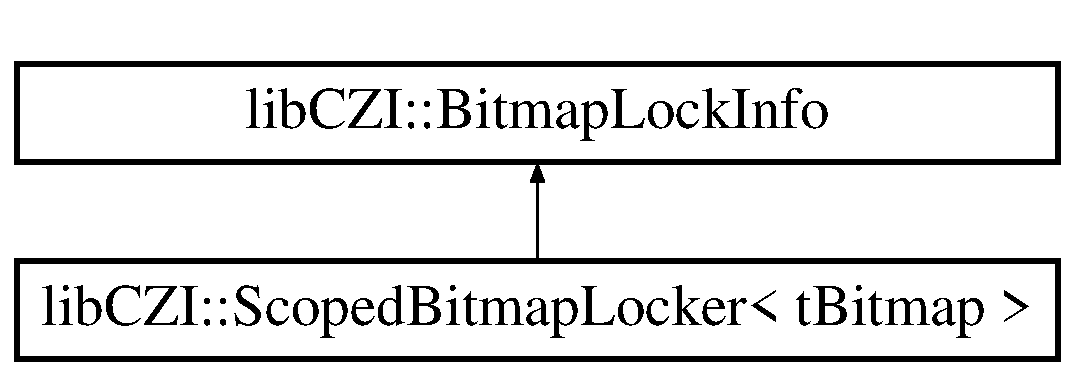
\includegraphics[height=2.000000cm]{structlib_c_z_i_1_1_bitmap_lock_info}
\end{center}
\end{figure}
\subsection*{Public Attributes}
\begin{DoxyCompactItemize}
\item 
\mbox{\Hypertarget{structlib_c_z_i_1_1_bitmap_lock_info_a1113106a82231213cd4e8980d3106ebd}\label{structlib_c_z_i_1_1_bitmap_lock_info_a1113106a82231213cd4e8980d3106ebd}} 
void $\ast$ \hyperlink{structlib_c_z_i_1_1_bitmap_lock_info_a1113106a82231213cd4e8980d3106ebd}{ptr\+Data}
\begin{DoxyCompactList}\small\item\em Not currently used, to be ignored. \end{DoxyCompactList}\item 
\mbox{\Hypertarget{structlib_c_z_i_1_1_bitmap_lock_info_ab54e2118992996eacc9ccd8e49397f09}\label{structlib_c_z_i_1_1_bitmap_lock_info_ab54e2118992996eacc9ccd8e49397f09}} 
void $\ast$ \hyperlink{structlib_c_z_i_1_1_bitmap_lock_info_ab54e2118992996eacc9ccd8e49397f09}{ptr\+Data\+Roi}
\begin{DoxyCompactList}\small\item\em The pointer to the first (top-\/left) pixel of the bitmap. \end{DoxyCompactList}\item 
\mbox{\Hypertarget{structlib_c_z_i_1_1_bitmap_lock_info_a8e7259142382ec0ad887c974d27775b6}\label{structlib_c_z_i_1_1_bitmap_lock_info_a8e7259142382ec0ad887c974d27775b6}} 
std\+::uint32\+\_\+t \hyperlink{structlib_c_z_i_1_1_bitmap_lock_info_a8e7259142382ec0ad887c974d27775b6}{stride}
\begin{DoxyCompactList}\small\item\em The stride of the bitmap data (pointed to by {\ttfamily ptr\+Data\+Roi}). \end{DoxyCompactList}\item 
\mbox{\Hypertarget{structlib_c_z_i_1_1_bitmap_lock_info_a109f8d69b48bc4398861217c375dee1b}\label{structlib_c_z_i_1_1_bitmap_lock_info_a109f8d69b48bc4398861217c375dee1b}} 
std\+::uint64\+\_\+t \hyperlink{structlib_c_z_i_1_1_bitmap_lock_info_a109f8d69b48bc4398861217c375dee1b}{size}
\begin{DoxyCompactList}\small\item\em The size of the bitmap data (pointed to by {\ttfamily ptr\+Data\+Roi}) in bytes. \end{DoxyCompactList}\end{DoxyCompactItemize}


\subsection{Detailed Description}
Information about a locked bitmap -\/ allowing direct access to the image data in memory. 

The documentation for this struct was generated from the following file\+:\begin{DoxyCompactItemize}
\item 
lib\+C\+Z\+I/lib\+C\+Z\+I\+\_\+\+Pixels.\+h\end{DoxyCompactItemize}

\hypertarget{structlib_c_z_i_1_1_bounding_boxes}{}\section{lib\+C\+ZI\+:\+:Bounding\+Boxes Struct Reference}
\label{structlib_c_z_i_1_1_bounding_boxes}\index{lib\+C\+Z\+I\+::\+Bounding\+Boxes@{lib\+C\+Z\+I\+::\+Bounding\+Boxes}}


This structure gathers the bounding-\/boxes determined from all sub-\/blocks and only be those on pyramid-\/layer 0.  




{\ttfamily \#include $<$lib\+C\+Z\+I.\+h$>$}

\subsection*{Public Attributes}
\begin{DoxyCompactItemize}
\item 
\mbox{\Hypertarget{structlib_c_z_i_1_1_bounding_boxes_abc2beea033eba496b26cbfdb4b16ced6}\label{structlib_c_z_i_1_1_bounding_boxes_abc2beea033eba496b26cbfdb4b16ced6}} 
\hyperlink{structlib_c_z_i_1_1_int_rect}{Int\+Rect} \hyperlink{structlib_c_z_i_1_1_bounding_boxes_abc2beea033eba496b26cbfdb4b16ced6}{bounding\+Box}
\begin{DoxyCompactList}\small\item\em The bounding-\/box determined from all sub-\/blocks. \end{DoxyCompactList}\item 
\mbox{\Hypertarget{structlib_c_z_i_1_1_bounding_boxes_a6e0e45a2c8bc35fe10463437dc8b9509}\label{structlib_c_z_i_1_1_bounding_boxes_a6e0e45a2c8bc35fe10463437dc8b9509}} 
\hyperlink{structlib_c_z_i_1_1_int_rect}{Int\+Rect} \hyperlink{structlib_c_z_i_1_1_bounding_boxes_a6e0e45a2c8bc35fe10463437dc8b9509}{bounding\+Box\+Layer0}
\begin{DoxyCompactList}\small\item\em The bounding-\/boxes determined only from sub-\/blocks of pyramid-\/layer 0. \end{DoxyCompactList}\end{DoxyCompactItemize}


\subsection{Detailed Description}
This structure gathers the bounding-\/boxes determined from all sub-\/blocks and only be those on pyramid-\/layer 0. 

The documentation for this struct was generated from the following file\+:\begin{DoxyCompactItemize}
\item 
lib\+C\+Z\+I/lib\+C\+Z\+I.\+h\end{DoxyCompactItemize}

\hypertarget{structlib_c_z_i_1_1_build_information}{}\section{lib\+C\+ZI\+:\+:Build\+Information Struct Reference}
\label{structlib_c_z_i_1_1_build_information}\index{lib\+C\+Z\+I\+::\+Build\+Information@{lib\+C\+Z\+I\+::\+Build\+Information}}


{\ttfamily \#include $<$lib\+C\+Z\+I.\+h$>$}

\subsection*{Public Attributes}
\begin{DoxyCompactItemize}
\item 
\mbox{\Hypertarget{structlib_c_z_i_1_1_build_information_afbe4e34c12ec00918b6c24cea02010fc}\label{structlib_c_z_i_1_1_build_information_afbe4e34c12ec00918b6c24cea02010fc}} 
std\+::string \hyperlink{structlib_c_z_i_1_1_build_information_afbe4e34c12ec00918b6c24cea02010fc}{compiler\+Identification}
\begin{DoxyCompactList}\small\item\em The compiler identification. This is a free-\/form string. \end{DoxyCompactList}\item 
\mbox{\Hypertarget{structlib_c_z_i_1_1_build_information_ade6220dd4d87b8cf00e3d49edde9d1cd}\label{structlib_c_z_i_1_1_build_information_ade6220dd4d87b8cf00e3d49edde9d1cd}} 
std\+::string \hyperlink{structlib_c_z_i_1_1_build_information_ade6220dd4d87b8cf00e3d49edde9d1cd}{repository\+Url}
\begin{DoxyCompactList}\small\item\em The U\+RL of the repository -\/ if available. \end{DoxyCompactList}\item 
\mbox{\Hypertarget{structlib_c_z_i_1_1_build_information_ae27730fdc6cc3c6061a600d6f32d75d5}\label{structlib_c_z_i_1_1_build_information_ae27730fdc6cc3c6061a600d6f32d75d5}} 
std\+::string \hyperlink{structlib_c_z_i_1_1_build_information_ae27730fdc6cc3c6061a600d6f32d75d5}{repository\+Branch}
\begin{DoxyCompactList}\small\item\em The branch -\/ if available. \end{DoxyCompactList}\item 
\mbox{\Hypertarget{structlib_c_z_i_1_1_build_information_a833dfce6058929d32f21133c46dc2f6d}\label{structlib_c_z_i_1_1_build_information_a833dfce6058929d32f21133c46dc2f6d}} 
std\+::string \hyperlink{structlib_c_z_i_1_1_build_information_a833dfce6058929d32f21133c46dc2f6d}{repository\+Tag}
\begin{DoxyCompactList}\small\item\em The tag or hash of the repository -\/ if available. \end{DoxyCompactList}\end{DoxyCompactItemize}


\subsection{Detailed Description}
This structure contains information about the compiler settings and the version of the source which was used to create the library. 

The documentation for this struct was generated from the following file\+:\begin{DoxyCompactItemize}
\item 
lib\+C\+Z\+I/lib\+C\+Z\+I.\+h\end{DoxyCompactItemize}

\hypertarget{classlib_c_z_i_1_1_c_dim_base}{}\section{lib\+C\+ZI\+:\+:C\+Dim\+Base Class Reference}
\label{classlib_c_z_i_1_1_c_dim_base}\index{lib\+C\+Z\+I\+::\+C\+Dim\+Base@{lib\+C\+Z\+I\+::\+C\+Dim\+Base}}


Base class containing some commonly used methods.  




{\ttfamily \#include $<$lib\+C\+Z\+I\+\_\+\+Dim\+Coordinate.\+h$>$}

Inheritance diagram for lib\+C\+ZI\+:\+:C\+Dim\+Base\+:\begin{figure}[H]
\begin{center}
\leavevmode
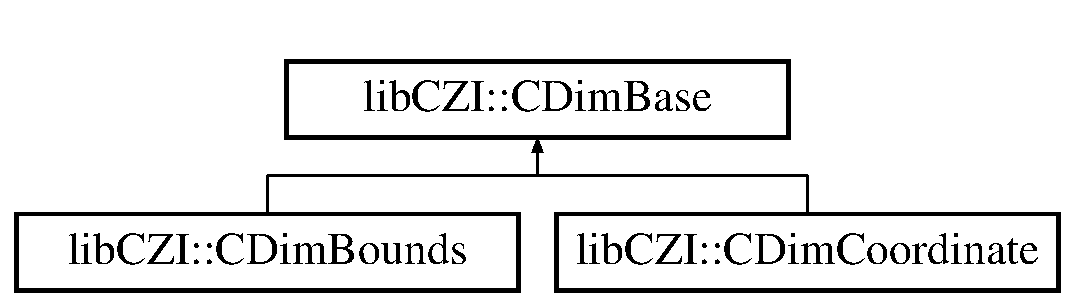
\includegraphics[height=2.000000cm]{classlib_c_z_i_1_1_c_dim_base}
\end{center}
\end{figure}
\subsection*{Static Protected Member Functions}
\begin{DoxyCompactItemize}
\item 
static std\+::underlying\+\_\+type$<$ \hyperlink{namespacelib_c_z_i_a55049658acf59d0eddfaebcad16df424}{lib\+C\+Z\+I\+::\+Dimension\+Index} $>$\+::type \hyperlink{classlib_c_z_i_1_1_c_dim_base_a952c7d14a037f1d6cf6d17ad15fac55a}{Get\+Bit\+Index\+For\+Dimension} (\hyperlink{namespacelib_c_z_i_a55049658acf59d0eddfaebcad16df424}{lib\+C\+Z\+I\+::\+Dimension\+Index} dim)
\end{DoxyCompactItemize}


\subsection{Detailed Description}
Base class containing some commonly used methods. 

\subsection{Member Function Documentation}
\mbox{\Hypertarget{classlib_c_z_i_1_1_c_dim_base_a952c7d14a037f1d6cf6d17ad15fac55a}\label{classlib_c_z_i_1_1_c_dim_base_a952c7d14a037f1d6cf6d17ad15fac55a}} 
\index{lib\+C\+Z\+I\+::\+C\+Dim\+Base@{lib\+C\+Z\+I\+::\+C\+Dim\+Base}!Get\+Bit\+Index\+For\+Dimension@{Get\+Bit\+Index\+For\+Dimension}}
\index{Get\+Bit\+Index\+For\+Dimension@{Get\+Bit\+Index\+For\+Dimension}!lib\+C\+Z\+I\+::\+C\+Dim\+Base@{lib\+C\+Z\+I\+::\+C\+Dim\+Base}}
\subsubsection{\texorpdfstring{Get\+Bit\+Index\+For\+Dimension()}{GetBitIndexForDimension()}}
{\footnotesize\ttfamily static std\+::underlying\+\_\+type$<$\hyperlink{namespacelib_c_z_i_a55049658acf59d0eddfaebcad16df424}{lib\+C\+Z\+I\+::\+Dimension\+Index}$>$\+::type lib\+C\+Z\+I\+::\+C\+Dim\+Base\+::\+Get\+Bit\+Index\+For\+Dimension (\begin{DoxyParamCaption}\item[{\hyperlink{namespacelib_c_z_i_a55049658acf59d0eddfaebcad16df424}{lib\+C\+Z\+I\+::\+Dimension\+Index}}]{dim }\end{DoxyParamCaption})\hspace{0.3cm}{\ttfamily [inline]}, {\ttfamily [static]}, {\ttfamily [protected]}}

Utility to get a bit index for the specified dimension. 
\begin{DoxyParams}{Parameters}
{\em dim} & The dimension. \\
\hline
\end{DoxyParams}
\begin{DoxyReturn}{Returns}
The bit index for dimension. 
\end{DoxyReturn}


The documentation for this class was generated from the following file\+:\begin{DoxyCompactItemize}
\item 
lib\+C\+Z\+I/lib\+C\+Z\+I\+\_\+\+Dim\+Coordinate.\+h\end{DoxyCompactItemize}

\hypertarget{classlib_c_z_i_1_1_c_dim_bounds}{}\section{lib\+C\+ZI\+:\+:C\+Dim\+Bounds Class Reference}
\label{classlib_c_z_i_1_1_c_dim_bounds}\index{lib\+C\+Z\+I\+::\+C\+Dim\+Bounds@{lib\+C\+Z\+I\+::\+C\+Dim\+Bounds}}


Implementation of a class representing an interval (and implementing the {\ttfamily \hyperlink{classlib_c_z_i_1_1_i_dim_bounds}{lib\+C\+Z\+I\+::\+I\+Dim\+Bounds}}-\/interface).  




{\ttfamily \#include $<$lib\+C\+Z\+I\+\_\+\+Dim\+Coordinate.\+h$>$}

Inheritance diagram for lib\+C\+ZI\+:\+:C\+Dim\+Bounds\+:\begin{figure}[H]
\begin{center}
\leavevmode
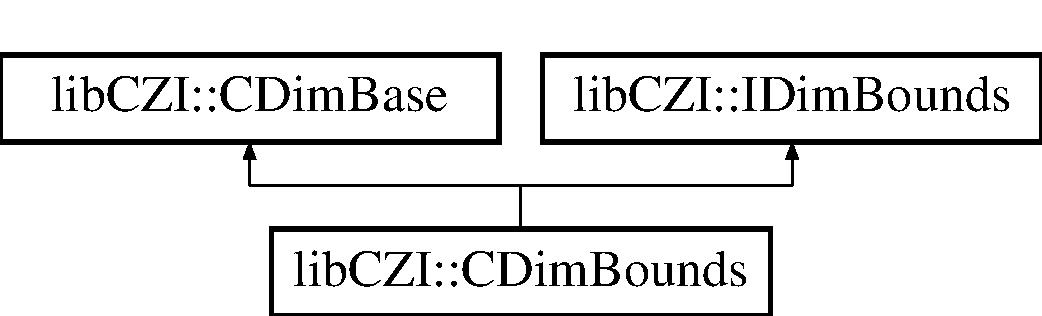
\includegraphics[height=2.000000cm]{classlib_c_z_i_1_1_c_dim_bounds}
\end{center}
\end{figure}
\subsection*{Public Member Functions}
\begin{DoxyCompactItemize}
\item 
\mbox{\Hypertarget{classlib_c_z_i_1_1_c_dim_bounds_a86cb06505f8ac0cf75a9258f49ef58dc}\label{classlib_c_z_i_1_1_c_dim_bounds_a86cb06505f8ac0cf75a9258f49ef58dc}} 
\hyperlink{classlib_c_z_i_1_1_c_dim_bounds_a86cb06505f8ac0cf75a9258f49ef58dc}{C\+Dim\+Bounds} ()
\begin{DoxyCompactList}\small\item\em Default constructor -\/ the object will contain no valid dimension. \end{DoxyCompactList}\item 
\hyperlink{classlib_c_z_i_1_1_c_dim_bounds_a176e01bb95a50cecf18f0e172937151e}{C\+Dim\+Bounds} (const \hyperlink{classlib_c_z_i_1_1_i_dim_bounds}{I\+Dim\+Bounds} $\ast$other)
\item 
\hyperlink{classlib_c_z_i_1_1_c_dim_bounds_aae378201c633fa582d3af0740b1b634a}{C\+Dim\+Bounds} (std\+::initializer\+\_\+list$<$ \hyperlink{structlib_c_z_i_1_1_dimension_and_start_size}{Dimension\+And\+Start\+Size} $>$ list)
\item 
void \hyperlink{classlib_c_z_i_1_1_c_dim_bounds_a7a872729a919b4573755032fbfdfc183}{Set} (\hyperlink{namespacelib_c_z_i_a55049658acf59d0eddfaebcad16df424}{lib\+C\+Z\+I\+::\+Dimension\+Index} dimension, int start, int size)
\item 
void \hyperlink{classlib_c_z_i_1_1_c_dim_bounds_ae2bddb983e507840449695dc2757cd2f}{Enum\+Valid\+Dimensions} (std\+::function$<$ bool(\hyperlink{namespacelib_c_z_i_a55049658acf59d0eddfaebcad16df424}{lib\+C\+Z\+I\+::\+Dimension\+Index} dim, int start, int size)$>$ func) const
\item 
void \hyperlink{classlib_c_z_i_1_1_c_dim_bounds_a96a5f7ec6f13896998eff3c7d2c7e5bf}{Clear} (\hyperlink{namespacelib_c_z_i_a55049658acf59d0eddfaebcad16df424}{lib\+C\+Z\+I\+::\+Dimension\+Index} dimension)
\item 
\mbox{\Hypertarget{classlib_c_z_i_1_1_c_dim_bounds_a7e84b9c941feefe65e2a4005a3c58e14}\label{classlib_c_z_i_1_1_c_dim_bounds_a7e84b9c941feefe65e2a4005a3c58e14}} 
void \hyperlink{classlib_c_z_i_1_1_c_dim_bounds_a7e84b9c941feefe65e2a4005a3c58e14}{Clear} ()
\begin{DoxyCompactList}\small\item\em Clears this object to its blank/initial state. All dimensions will be set to invalid. \end{DoxyCompactList}\item 
bool \hyperlink{classlib_c_z_i_1_1_c_dim_bounds_a8c72a9198f5b88b1d3d68acdb79758ba}{Is\+Empty} () const
\item 
virtual bool \hyperlink{classlib_c_z_i_1_1_c_dim_bounds_abf42285e28ddc4843556f88b2292c494}{Try\+Get\+Interval} (\hyperlink{namespacelib_c_z_i_a55049658acf59d0eddfaebcad16df424}{lib\+C\+Z\+I\+::\+Dimension\+Index} dim, int $\ast$start\+Index, int $\ast$size) const
\end{DoxyCompactItemize}
\subsection*{Static Public Member Functions}
\begin{DoxyCompactItemize}
\item 
static \hyperlink{classlib_c_z_i_1_1_c_dim_bounds}{C\+Dim\+Bounds} \hyperlink{classlib_c_z_i_1_1_c_dim_bounds_a10a59c07b8f3cb2ec8d8a082e9167bfb}{Parse} (const char $\ast$str)
\end{DoxyCompactItemize}
\subsection*{Additional Inherited Members}


\subsection{Detailed Description}
Implementation of a class representing an interval (and implementing the {\ttfamily \hyperlink{classlib_c_z_i_1_1_i_dim_bounds}{lib\+C\+Z\+I\+::\+I\+Dim\+Bounds}}-\/interface). 

\subsection{Constructor \& Destructor Documentation}
\mbox{\Hypertarget{classlib_c_z_i_1_1_c_dim_bounds_a176e01bb95a50cecf18f0e172937151e}\label{classlib_c_z_i_1_1_c_dim_bounds_a176e01bb95a50cecf18f0e172937151e}} 
\index{lib\+C\+Z\+I\+::\+C\+Dim\+Bounds@{lib\+C\+Z\+I\+::\+C\+Dim\+Bounds}!C\+Dim\+Bounds@{C\+Dim\+Bounds}}
\index{C\+Dim\+Bounds@{C\+Dim\+Bounds}!lib\+C\+Z\+I\+::\+C\+Dim\+Bounds@{lib\+C\+Z\+I\+::\+C\+Dim\+Bounds}}
\subsubsection{\texorpdfstring{C\+Dim\+Bounds()}{CDimBounds()}\hspace{0.1cm}{\footnotesize\ttfamily [1/2]}}
{\footnotesize\ttfamily lib\+C\+Z\+I\+::\+C\+Dim\+Bounds\+::\+C\+Dim\+Bounds (\begin{DoxyParamCaption}\item[{const \hyperlink{classlib_c_z_i_1_1_i_dim_bounds}{I\+Dim\+Bounds} $\ast$}]{other }\end{DoxyParamCaption})\hspace{0.3cm}{\ttfamily [inline]}}

Constructor which copies the content of the specified I\+Dim\+Bounds-\/object.


\begin{DoxyParams}{Parameters}
{\em other} & The I\+Dim\+Bounds-\/object to copy information from. \\
\hline
\end{DoxyParams}
\mbox{\Hypertarget{classlib_c_z_i_1_1_c_dim_bounds_aae378201c633fa582d3af0740b1b634a}\label{classlib_c_z_i_1_1_c_dim_bounds_aae378201c633fa582d3af0740b1b634a}} 
\index{lib\+C\+Z\+I\+::\+C\+Dim\+Bounds@{lib\+C\+Z\+I\+::\+C\+Dim\+Bounds}!C\+Dim\+Bounds@{C\+Dim\+Bounds}}
\index{C\+Dim\+Bounds@{C\+Dim\+Bounds}!lib\+C\+Z\+I\+::\+C\+Dim\+Bounds@{lib\+C\+Z\+I\+::\+C\+Dim\+Bounds}}
\subsubsection{\texorpdfstring{C\+Dim\+Bounds()}{CDimBounds()}\hspace{0.1cm}{\footnotesize\ttfamily [2/2]}}
{\footnotesize\ttfamily lib\+C\+Z\+I\+::\+C\+Dim\+Bounds\+::\+C\+Dim\+Bounds (\begin{DoxyParamCaption}\item[{std\+::initializer\+\_\+list$<$ \hyperlink{structlib_c_z_i_1_1_dimension_and_start_size}{Dimension\+And\+Start\+Size} $>$}]{list }\end{DoxyParamCaption})\hspace{0.3cm}{\ttfamily [inline]}}

Construct a \hyperlink{classlib_c_z_i_1_1_c_dim_bounds}{lib\+C\+Z\+I\+::\+C\+Dim\+Bounds} object from an initializer-\/list. 
\begin{DoxyParams}{Parameters}
{\em list} & The list of \char`\"{}dimension, start and size\char`\"{}. \\
\hline
\end{DoxyParams}


\subsection{Member Function Documentation}
\mbox{\Hypertarget{classlib_c_z_i_1_1_c_dim_bounds_a96a5f7ec6f13896998eff3c7d2c7e5bf}\label{classlib_c_z_i_1_1_c_dim_bounds_a96a5f7ec6f13896998eff3c7d2c7e5bf}} 
\index{lib\+C\+Z\+I\+::\+C\+Dim\+Bounds@{lib\+C\+Z\+I\+::\+C\+Dim\+Bounds}!Clear@{Clear}}
\index{Clear@{Clear}!lib\+C\+Z\+I\+::\+C\+Dim\+Bounds@{lib\+C\+Z\+I\+::\+C\+Dim\+Bounds}}
\subsubsection{\texorpdfstring{Clear()}{Clear()}}
{\footnotesize\ttfamily void lib\+C\+Z\+I\+::\+C\+Dim\+Bounds\+::\+Clear (\begin{DoxyParamCaption}\item[{\hyperlink{namespacelib_c_z_i_a55049658acf59d0eddfaebcad16df424}{lib\+C\+Z\+I\+::\+Dimension\+Index}}]{dimension }\end{DoxyParamCaption})\hspace{0.3cm}{\ttfamily [inline]}}

Clears the validity of the specified dimension. 
\begin{DoxyParams}{Parameters}
{\em dimension} & The dimension. \\
\hline
\end{DoxyParams}
\mbox{\Hypertarget{classlib_c_z_i_1_1_c_dim_bounds_ae2bddb983e507840449695dc2757cd2f}\label{classlib_c_z_i_1_1_c_dim_bounds_ae2bddb983e507840449695dc2757cd2f}} 
\index{lib\+C\+Z\+I\+::\+C\+Dim\+Bounds@{lib\+C\+Z\+I\+::\+C\+Dim\+Bounds}!Enum\+Valid\+Dimensions@{Enum\+Valid\+Dimensions}}
\index{Enum\+Valid\+Dimensions@{Enum\+Valid\+Dimensions}!lib\+C\+Z\+I\+::\+C\+Dim\+Bounds@{lib\+C\+Z\+I\+::\+C\+Dim\+Bounds}}
\subsubsection{\texorpdfstring{Enum\+Valid\+Dimensions()}{EnumValidDimensions()}}
{\footnotesize\ttfamily void lib\+C\+Z\+I\+::\+C\+Dim\+Bounds\+::\+Enum\+Valid\+Dimensions (\begin{DoxyParamCaption}\item[{std\+::function$<$ bool(\hyperlink{namespacelib_c_z_i_a55049658acf59d0eddfaebcad16df424}{lib\+C\+Z\+I\+::\+Dimension\+Index} dim, int start, int size)$>$}]{func }\end{DoxyParamCaption}) const\hspace{0.3cm}{\ttfamily [inline]}}

Enumerate valid dimensions. 
\begin{DoxyParams}{Parameters}
{\em func} & The functor which will be called for all valid dimensions. \\
\hline
\end{DoxyParams}
\mbox{\Hypertarget{classlib_c_z_i_1_1_c_dim_bounds_a8c72a9198f5b88b1d3d68acdb79758ba}\label{classlib_c_z_i_1_1_c_dim_bounds_a8c72a9198f5b88b1d3d68acdb79758ba}} 
\index{lib\+C\+Z\+I\+::\+C\+Dim\+Bounds@{lib\+C\+Z\+I\+::\+C\+Dim\+Bounds}!Is\+Empty@{Is\+Empty}}
\index{Is\+Empty@{Is\+Empty}!lib\+C\+Z\+I\+::\+C\+Dim\+Bounds@{lib\+C\+Z\+I\+::\+C\+Dim\+Bounds}}
\subsubsection{\texorpdfstring{Is\+Empty()}{IsEmpty()}}
{\footnotesize\ttfamily bool lib\+C\+Z\+I\+::\+C\+Dim\+Bounds\+::\+Is\+Empty (\begin{DoxyParamCaption}{ }\end{DoxyParamCaption}) const\hspace{0.3cm}{\ttfamily [inline]}}

Query if this object is empty -\/ no valid dimensions contained.

\begin{DoxyReturn}{Returns}
True if empty, false if not. 
\end{DoxyReturn}
\mbox{\Hypertarget{classlib_c_z_i_1_1_c_dim_bounds_a10a59c07b8f3cb2ec8d8a082e9167bfb}\label{classlib_c_z_i_1_1_c_dim_bounds_a10a59c07b8f3cb2ec8d8a082e9167bfb}} 
\index{lib\+C\+Z\+I\+::\+C\+Dim\+Bounds@{lib\+C\+Z\+I\+::\+C\+Dim\+Bounds}!Parse@{Parse}}
\index{Parse@{Parse}!lib\+C\+Z\+I\+::\+C\+Dim\+Bounds@{lib\+C\+Z\+I\+::\+C\+Dim\+Bounds}}
\subsubsection{\texorpdfstring{Parse()}{Parse()}}
{\footnotesize\ttfamily static \hyperlink{classlib_c_z_i_1_1_c_dim_bounds}{C\+Dim\+Bounds} lib\+C\+Z\+I\+::\+C\+Dim\+Bounds\+::\+Parse (\begin{DoxyParamCaption}\item[{const char $\ast$}]{str }\end{DoxyParamCaption})\hspace{0.3cm}{\ttfamily [static]}}

Parse the specified string and construct a C\+Dim\+Bounds-\/object from the information. The syntax for the string is -\/ a character identifying the dimension (one of \textquotesingle{}Z\textquotesingle{}, \textquotesingle{}C\textquotesingle{}, \textquotesingle{}T\textquotesingle{}, \textquotesingle{}R\textquotesingle{}, \textquotesingle{}S\textquotesingle{}, \textquotesingle{}I\textquotesingle{}, \textquotesingle{}H\textquotesingle{}, \textquotesingle{}V\textquotesingle{}, \textquotesingle{}B\textquotesingle{}) followed by an integer (possibly with a + or -\/) specifying the start-\/index, followed by a colon \textquotesingle{}\+:\textquotesingle{}, then followed by an integer specifying the size. There can be more than one dimension given, in which case the above sequence is repeated for a different dimension. It is illegal to give the same dimension multiple times. Examples\+: \char`\"{}\+T0\+:10\char`\"{}, \char`\"{}\+T0\+:5\+Z0\+:10\char`\"{}, \char`\"{}\+C0\+:2\+T0\+:10\+Z0\+:5\char`\"{}.


\begin{DoxyExceptions}{Exceptions}
{\em \hyperlink{classlib_c_z_i_1_1_lib_c_z_i_string_parse_exception}{Lib\+C\+Z\+I\+String\+Parse\+Exception}} & Thrown when the specified string cannot be parsed because of a syntactical error.\\
\hline
\end{DoxyExceptions}

\begin{DoxyParams}{Parameters}
{\em str} & The string to parse.\\
\hline
\end{DoxyParams}
\begin{DoxyReturn}{Returns}
A \hyperlink{classlib_c_z_i_1_1_c_dim_bounds}{C\+Dim\+Bounds} object constructed from the string. 
\end{DoxyReturn}
\mbox{\Hypertarget{classlib_c_z_i_1_1_c_dim_bounds_a7a872729a919b4573755032fbfdfc183}\label{classlib_c_z_i_1_1_c_dim_bounds_a7a872729a919b4573755032fbfdfc183}} 
\index{lib\+C\+Z\+I\+::\+C\+Dim\+Bounds@{lib\+C\+Z\+I\+::\+C\+Dim\+Bounds}!Set@{Set}}
\index{Set@{Set}!lib\+C\+Z\+I\+::\+C\+Dim\+Bounds@{lib\+C\+Z\+I\+::\+C\+Dim\+Bounds}}
\subsubsection{\texorpdfstring{Set()}{Set()}}
{\footnotesize\ttfamily void lib\+C\+Z\+I\+::\+C\+Dim\+Bounds\+::\+Set (\begin{DoxyParamCaption}\item[{\hyperlink{namespacelib_c_z_i_a55049658acf59d0eddfaebcad16df424}{lib\+C\+Z\+I\+::\+Dimension\+Index}}]{dimension,  }\item[{int}]{start,  }\item[{int}]{size }\end{DoxyParamCaption})\hspace{0.3cm}{\ttfamily [inline]}}

Sets (for the specified dimension) the start and the size. 
\begin{DoxyParams}{Parameters}
{\em dimension} & The dimension. \\
\hline
{\em start} & The start. \\
\hline
{\em size} & The size. \\
\hline
\end{DoxyParams}
\mbox{\Hypertarget{classlib_c_z_i_1_1_c_dim_bounds_abf42285e28ddc4843556f88b2292c494}\label{classlib_c_z_i_1_1_c_dim_bounds_abf42285e28ddc4843556f88b2292c494}} 
\index{lib\+C\+Z\+I\+::\+C\+Dim\+Bounds@{lib\+C\+Z\+I\+::\+C\+Dim\+Bounds}!Try\+Get\+Interval@{Try\+Get\+Interval}}
\index{Try\+Get\+Interval@{Try\+Get\+Interval}!lib\+C\+Z\+I\+::\+C\+Dim\+Bounds@{lib\+C\+Z\+I\+::\+C\+Dim\+Bounds}}
\subsubsection{\texorpdfstring{Try\+Get\+Interval()}{TryGetInterval()}}
{\footnotesize\ttfamily virtual bool lib\+C\+Z\+I\+::\+C\+Dim\+Bounds\+::\+Try\+Get\+Interval (\begin{DoxyParamCaption}\item[{\hyperlink{namespacelib_c_z_i_a55049658acf59d0eddfaebcad16df424}{lib\+C\+Z\+I\+::\+Dimension\+Index}}]{dim,  }\item[{int $\ast$}]{start\+Index,  }\item[{int $\ast$}]{size }\end{DoxyParamCaption}) const\hspace{0.3cm}{\ttfamily [inline]}, {\ttfamily [virtual]}}

Attempts to get interval and size for the specified dimension. 
\begin{DoxyParams}[1]{Parameters}
 & {\em dim} & The dimemension. \\
\hline
\mbox{\tt out}  & {\em start\+Index} & If non-\/null, it will receive the start index. \\
\hline
\mbox{\tt out}  & {\em size} & If non-\/null, it will receive the size. \\
\hline
\end{DoxyParams}
\begin{DoxyReturn}{Returns}
True if it succeeds, false if it fails. 
\end{DoxyReturn}


Implements \hyperlink{classlib_c_z_i_1_1_i_dim_bounds_a7f42cf193370731a6b21ae5d2d6fa78e}{lib\+C\+Z\+I\+::\+I\+Dim\+Bounds}.



The documentation for this class was generated from the following file\+:\begin{DoxyCompactItemize}
\item 
lib\+C\+Z\+I/lib\+C\+Z\+I\+\_\+\+Dim\+Coordinate.\+h\end{DoxyCompactItemize}

\hypertarget{classlib_c_z_i_1_1_c_dim_coordinate}{}\section{lib\+C\+ZI\+:\+:C\+Dim\+Coordinate Class Reference}
\label{classlib_c_z_i_1_1_c_dim_coordinate}\index{lib\+C\+Z\+I\+::\+C\+Dim\+Coordinate@{lib\+C\+Z\+I\+::\+C\+Dim\+Coordinate}}


Implementation of a class representing a coordinate (and implementing the {\ttfamily \hyperlink{classlib_c_z_i_1_1_i_dim_coordinate}{I\+Dim\+Coordinate}}-\/interface).  




{\ttfamily \#include $<$lib\+C\+Z\+I\+\_\+\+Dim\+Coordinate.\+h$>$}

Inheritance diagram for lib\+C\+ZI\+:\+:C\+Dim\+Coordinate\+:\begin{figure}[H]
\begin{center}
\leavevmode
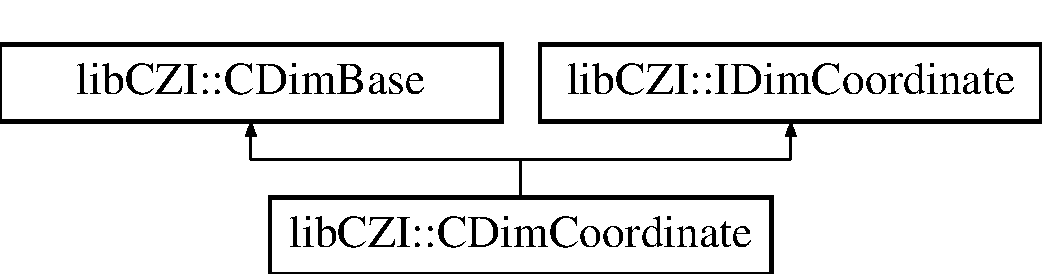
\includegraphics[height=2.000000cm]{classlib_c_z_i_1_1_c_dim_coordinate}
\end{center}
\end{figure}
\subsection*{Public Member Functions}
\begin{DoxyCompactItemize}
\item 
\mbox{\Hypertarget{classlib_c_z_i_1_1_c_dim_coordinate_a51d381d8965a8d10c6d0295593bc3885}\label{classlib_c_z_i_1_1_c_dim_coordinate_a51d381d8965a8d10c6d0295593bc3885}} 
\hyperlink{classlib_c_z_i_1_1_c_dim_coordinate_a51d381d8965a8d10c6d0295593bc3885}{C\+Dim\+Coordinate} ()
\begin{DoxyCompactList}\small\item\em Default constructor which constructs an empty coordinate (no valid dimensions). \end{DoxyCompactList}\item 
\hyperlink{classlib_c_z_i_1_1_c_dim_coordinate_a513ae54e9dc32c0c19040b94add75e80}{C\+Dim\+Coordinate} (std\+::initializer\+\_\+list$<$ \hyperlink{structlib_c_z_i_1_1_dimension_and_value}{Dimension\+And\+Value} $>$ list)
\item 
\hyperlink{classlib_c_z_i_1_1_c_dim_coordinate_a95be8c1ca51e6bf4e5efc4f23a027148}{C\+Dim\+Coordinate} (const \hyperlink{classlib_c_z_i_1_1_i_dim_coordinate}{lib\+C\+Z\+I\+::\+I\+Dim\+Coordinate} $\ast$other)
\item 
void \hyperlink{classlib_c_z_i_1_1_c_dim_coordinate_a9f6d967df6c2040e395c0710e8374909}{Set} (\hyperlink{namespacelib_c_z_i_a55049658acf59d0eddfaebcad16df424}{lib\+C\+Z\+I\+::\+Dimension\+Index} dimension, int value)
\item 
void \hyperlink{classlib_c_z_i_1_1_c_dim_coordinate_abfffd501e6cb4818a4b0454920b866ef}{Clear} (\hyperlink{namespacelib_c_z_i_a55049658acf59d0eddfaebcad16df424}{lib\+C\+Z\+I\+::\+Dimension\+Index} dimension)
\item 
\mbox{\Hypertarget{classlib_c_z_i_1_1_c_dim_coordinate_ae1a5a2f981dff4c66edd2a4ef86829ef}\label{classlib_c_z_i_1_1_c_dim_coordinate_ae1a5a2f981dff4c66edd2a4ef86829ef}} 
void \hyperlink{classlib_c_z_i_1_1_c_dim_coordinate_ae1a5a2f981dff4c66edd2a4ef86829ef}{Clear} ()
\begin{DoxyCompactList}\small\item\em Clears the validity of all dimensions. \end{DoxyCompactList}\item 
void \hyperlink{classlib_c_z_i_1_1_c_dim_coordinate_a65d3104fbc171cdab0cd53616df13f8e}{Enum\+Valid\+Dimensions} (std\+::function$<$ bool(\hyperlink{namespacelib_c_z_i_a55049658acf59d0eddfaebcad16df424}{lib\+C\+Z\+I\+::\+Dimension\+Index} dim, int value)$>$ func) const
\item 
\mbox{\Hypertarget{classlib_c_z_i_1_1_c_dim_coordinate_a94b1116ff62dc82965df419b46e73dac}\label{classlib_c_z_i_1_1_c_dim_coordinate_a94b1116ff62dc82965df419b46e73dac}} 
int \hyperlink{classlib_c_z_i_1_1_c_dim_coordinate_a94b1116ff62dc82965df419b46e73dac}{Get\+Valid\+Dimensions\+Count} () const
\begin{DoxyCompactList}\small\item\em Determine the number the valid dimensions contained in this coordinate. \end{DoxyCompactList}\item 
virtual bool \hyperlink{classlib_c_z_i_1_1_c_dim_coordinate_af7bc7e775a5971d46550e45ebf2b2ba7}{Try\+Get\+Position} (\hyperlink{namespacelib_c_z_i_a55049658acf59d0eddfaebcad16df424}{lib\+C\+Z\+I\+::\+Dimension\+Index} dim, int $\ast$coordinate) const
\end{DoxyCompactItemize}
\subsection*{Static Public Member Functions}
\begin{DoxyCompactItemize}
\item 
static \hyperlink{classlib_c_z_i_1_1_c_dim_coordinate}{C\+Dim\+Coordinate} \hyperlink{classlib_c_z_i_1_1_c_dim_coordinate_a684c17ad37de1e817c660e89e704d81e}{Parse} (const char $\ast$str)
\end{DoxyCompactItemize}
\subsection*{Additional Inherited Members}


\subsection{Detailed Description}
Implementation of a class representing a coordinate (and implementing the {\ttfamily \hyperlink{classlib_c_z_i_1_1_i_dim_coordinate}{I\+Dim\+Coordinate}}-\/interface). 

\subsection{Constructor \& Destructor Documentation}
\mbox{\Hypertarget{classlib_c_z_i_1_1_c_dim_coordinate_a513ae54e9dc32c0c19040b94add75e80}\label{classlib_c_z_i_1_1_c_dim_coordinate_a513ae54e9dc32c0c19040b94add75e80}} 
\index{lib\+C\+Z\+I\+::\+C\+Dim\+Coordinate@{lib\+C\+Z\+I\+::\+C\+Dim\+Coordinate}!C\+Dim\+Coordinate@{C\+Dim\+Coordinate}}
\index{C\+Dim\+Coordinate@{C\+Dim\+Coordinate}!lib\+C\+Z\+I\+::\+C\+Dim\+Coordinate@{lib\+C\+Z\+I\+::\+C\+Dim\+Coordinate}}
\subsubsection{\texorpdfstring{C\+Dim\+Coordinate()}{CDimCoordinate()}\hspace{0.1cm}{\footnotesize\ttfamily [1/2]}}
{\footnotesize\ttfamily lib\+C\+Z\+I\+::\+C\+Dim\+Coordinate\+::\+C\+Dim\+Coordinate (\begin{DoxyParamCaption}\item[{std\+::initializer\+\_\+list$<$ \hyperlink{structlib_c_z_i_1_1_dimension_and_value}{Dimension\+And\+Value} $>$}]{list }\end{DoxyParamCaption})\hspace{0.3cm}{\ttfamily [inline]}}

Constructor which constructs a coordinate object from the specified initializer list. It can be used like this\+: 
\begin{DoxyCode}
\textcolor{keyword}{auto} coord = \hyperlink{classlib_c_z_i_1_1_c_dim_coordinate_a51d381d8965a8d10c6d0295593bc3885}{CDimCoordinate}\{ \{ \hyperlink{namespacelib_c_z_i_a55049658acf59d0eddfaebcad16df424a21c2e59531c8710156d34a3c30ac81d5}{DimensionIndex::Z},8 \} , \{ 
      \hyperlink{namespacelib_c_z_i_a55049658acf59d0eddfaebcad16df424ab9ece18c950afbfa6b0fdbfa4ff731d3}{DimensionIndex::T},0 \}, \{ \hyperlink{namespacelib_c_z_i_a55049658acf59d0eddfaebcad16df424a0d61f8370cad1d412f80b84d143e1257}{DimensionIndex::C},1 \} \};
\end{DoxyCode}
 \begin{DoxyRemark}{Remarks}
If the same dimension appears multiple times in the initializer list, then the last occurence wins. 
\end{DoxyRemark}

\begin{DoxyParams}{Parameters}
{\em list} & The list of dimensions-\/and-\/values. \\
\hline
\end{DoxyParams}
\mbox{\Hypertarget{classlib_c_z_i_1_1_c_dim_coordinate_a95be8c1ca51e6bf4e5efc4f23a027148}\label{classlib_c_z_i_1_1_c_dim_coordinate_a95be8c1ca51e6bf4e5efc4f23a027148}} 
\index{lib\+C\+Z\+I\+::\+C\+Dim\+Coordinate@{lib\+C\+Z\+I\+::\+C\+Dim\+Coordinate}!C\+Dim\+Coordinate@{C\+Dim\+Coordinate}}
\index{C\+Dim\+Coordinate@{C\+Dim\+Coordinate}!lib\+C\+Z\+I\+::\+C\+Dim\+Coordinate@{lib\+C\+Z\+I\+::\+C\+Dim\+Coordinate}}
\subsubsection{\texorpdfstring{C\+Dim\+Coordinate()}{CDimCoordinate()}\hspace{0.1cm}{\footnotesize\ttfamily [2/2]}}
{\footnotesize\ttfamily lib\+C\+Z\+I\+::\+C\+Dim\+Coordinate\+::\+C\+Dim\+Coordinate (\begin{DoxyParamCaption}\item[{const \hyperlink{classlib_c_z_i_1_1_i_dim_coordinate}{lib\+C\+Z\+I\+::\+I\+Dim\+Coordinate} $\ast$}]{other }\end{DoxyParamCaption})\hspace{0.3cm}{\ttfamily [inline]}}

Copy-\/constructor which creates a copy of the specifed coordinate.


\begin{DoxyParams}{Parameters}
{\em other} & The coordinate for which to create a copy. It may be null in which case an empty coordinate is created. \\
\hline
\end{DoxyParams}


\subsection{Member Function Documentation}
\mbox{\Hypertarget{classlib_c_z_i_1_1_c_dim_coordinate_abfffd501e6cb4818a4b0454920b866ef}\label{classlib_c_z_i_1_1_c_dim_coordinate_abfffd501e6cb4818a4b0454920b866ef}} 
\index{lib\+C\+Z\+I\+::\+C\+Dim\+Coordinate@{lib\+C\+Z\+I\+::\+C\+Dim\+Coordinate}!Clear@{Clear}}
\index{Clear@{Clear}!lib\+C\+Z\+I\+::\+C\+Dim\+Coordinate@{lib\+C\+Z\+I\+::\+C\+Dim\+Coordinate}}
\subsubsection{\texorpdfstring{Clear()}{Clear()}}
{\footnotesize\ttfamily void lib\+C\+Z\+I\+::\+C\+Dim\+Coordinate\+::\+Clear (\begin{DoxyParamCaption}\item[{\hyperlink{namespacelib_c_z_i_a55049658acf59d0eddfaebcad16df424}{lib\+C\+Z\+I\+::\+Dimension\+Index}}]{dimension }\end{DoxyParamCaption})\hspace{0.3cm}{\ttfamily [inline]}}

Clears the validity of the specified dimension.


\begin{DoxyParams}{Parameters}
{\em dimension} & The dimension to mark as \textquotesingle{}not valid for this coordinate\textquotesingle{}. \\
\hline
\end{DoxyParams}
\mbox{\Hypertarget{classlib_c_z_i_1_1_c_dim_coordinate_a65d3104fbc171cdab0cd53616df13f8e}\label{classlib_c_z_i_1_1_c_dim_coordinate_a65d3104fbc171cdab0cd53616df13f8e}} 
\index{lib\+C\+Z\+I\+::\+C\+Dim\+Coordinate@{lib\+C\+Z\+I\+::\+C\+Dim\+Coordinate}!Enum\+Valid\+Dimensions@{Enum\+Valid\+Dimensions}}
\index{Enum\+Valid\+Dimensions@{Enum\+Valid\+Dimensions}!lib\+C\+Z\+I\+::\+C\+Dim\+Coordinate@{lib\+C\+Z\+I\+::\+C\+Dim\+Coordinate}}
\subsubsection{\texorpdfstring{Enum\+Valid\+Dimensions()}{EnumValidDimensions()}}
{\footnotesize\ttfamily void lib\+C\+Z\+I\+::\+C\+Dim\+Coordinate\+::\+Enum\+Valid\+Dimensions (\begin{DoxyParamCaption}\item[{std\+::function$<$ bool(\hyperlink{namespacelib_c_z_i_a55049658acf59d0eddfaebcad16df424}{lib\+C\+Z\+I\+::\+Dimension\+Index} dim, int value)$>$}]{func }\end{DoxyParamCaption}) const\hspace{0.3cm}{\ttfamily [inline]}}

Enumerate the valid dimensions contained in this coordinate. The specified functor will be called for each valid dimension (and providing the functor with the dimension index and the coordinate). If the functor returns false, the enumeration is cancelled.


\begin{DoxyParams}{Parameters}
{\em func} & The functor to call for each valid dimension. If returning false, the enumeration is cancelled. \\
\hline
\end{DoxyParams}
\mbox{\Hypertarget{classlib_c_z_i_1_1_c_dim_coordinate_a684c17ad37de1e817c660e89e704d81e}\label{classlib_c_z_i_1_1_c_dim_coordinate_a684c17ad37de1e817c660e89e704d81e}} 
\index{lib\+C\+Z\+I\+::\+C\+Dim\+Coordinate@{lib\+C\+Z\+I\+::\+C\+Dim\+Coordinate}!Parse@{Parse}}
\index{Parse@{Parse}!lib\+C\+Z\+I\+::\+C\+Dim\+Coordinate@{lib\+C\+Z\+I\+::\+C\+Dim\+Coordinate}}
\subsubsection{\texorpdfstring{Parse()}{Parse()}}
{\footnotesize\ttfamily static \hyperlink{classlib_c_z_i_1_1_c_dim_coordinate}{C\+Dim\+Coordinate} lib\+C\+Z\+I\+::\+C\+Dim\+Coordinate\+::\+Parse (\begin{DoxyParamCaption}\item[{const char $\ast$}]{str }\end{DoxyParamCaption})\hspace{0.3cm}{\ttfamily [static]}}

Parse the specified string and construct a C\+Dim\+Coordinate-\/object from the information. The syntax for the string is -\/ a character identifying the dimension (one of \textquotesingle{}Z\textquotesingle{}, \textquotesingle{}C\textquotesingle{}, \textquotesingle{}T\textquotesingle{}, \textquotesingle{}R\textquotesingle{}, \textquotesingle{}S\textquotesingle{}, \textquotesingle{}I\textquotesingle{}, \textquotesingle{}H\textquotesingle{}, \textquotesingle{}V\textquotesingle{}, \textquotesingle{}B\textquotesingle{}) followed by an integer (possibly with a + or -\/). There can be more than one dimension given, in which case the parts can be separated by a comma, a semicolon or spaces. The regular expression is\+: 
\begin{DoxyCode}
([:blank:]*[Z|C|T|R|S|I|H|V|B][\(\backslash\)\(\backslash\)+|-]?[[:digit:]]+[,|;| ]*)
\end{DoxyCode}
 It is illegal to give the same dimension multiple times.


\begin{DoxyExceptions}{Exceptions}
{\em \hyperlink{classlib_c_z_i_1_1_lib_c_z_i_string_parse_exception}{Lib\+C\+Z\+I\+String\+Parse\+Exception}} & Thrown when the specified string cannot be parsed because of a syntactical error.\\
\hline
\end{DoxyExceptions}

\begin{DoxyParams}{Parameters}
{\em str} & The string to parse.\\
\hline
\end{DoxyParams}
\begin{DoxyReturn}{Returns}
A \hyperlink{classlib_c_z_i_1_1_c_dim_coordinate}{C\+Dim\+Coordinate} object constructed from the string. 
\end{DoxyReturn}
\mbox{\Hypertarget{classlib_c_z_i_1_1_c_dim_coordinate_a9f6d967df6c2040e395c0710e8374909}\label{classlib_c_z_i_1_1_c_dim_coordinate_a9f6d967df6c2040e395c0710e8374909}} 
\index{lib\+C\+Z\+I\+::\+C\+Dim\+Coordinate@{lib\+C\+Z\+I\+::\+C\+Dim\+Coordinate}!Set@{Set}}
\index{Set@{Set}!lib\+C\+Z\+I\+::\+C\+Dim\+Coordinate@{lib\+C\+Z\+I\+::\+C\+Dim\+Coordinate}}
\subsubsection{\texorpdfstring{Set()}{Set()}}
{\footnotesize\ttfamily void lib\+C\+Z\+I\+::\+C\+Dim\+Coordinate\+::\+Set (\begin{DoxyParamCaption}\item[{\hyperlink{namespacelib_c_z_i_a55049658acf59d0eddfaebcad16df424}{lib\+C\+Z\+I\+::\+Dimension\+Index}}]{dimension,  }\item[{int}]{value }\end{DoxyParamCaption})\hspace{0.3cm}{\ttfamily [inline]}}

Sets the value for the specified dimension. The specified dimension will be marked \textquotesingle{}valid\textquotesingle{}.


\begin{DoxyParams}{Parameters}
{\em dimension} & The dimension to set. \\
\hline
{\em value} & The value to set. \\
\hline
\end{DoxyParams}
\mbox{\Hypertarget{classlib_c_z_i_1_1_c_dim_coordinate_af7bc7e775a5971d46550e45ebf2b2ba7}\label{classlib_c_z_i_1_1_c_dim_coordinate_af7bc7e775a5971d46550e45ebf2b2ba7}} 
\index{lib\+C\+Z\+I\+::\+C\+Dim\+Coordinate@{lib\+C\+Z\+I\+::\+C\+Dim\+Coordinate}!Try\+Get\+Position@{Try\+Get\+Position}}
\index{Try\+Get\+Position@{Try\+Get\+Position}!lib\+C\+Z\+I\+::\+C\+Dim\+Coordinate@{lib\+C\+Z\+I\+::\+C\+Dim\+Coordinate}}
\subsubsection{\texorpdfstring{Try\+Get\+Position()}{TryGetPosition()}}
{\footnotesize\ttfamily virtual bool lib\+C\+Z\+I\+::\+C\+Dim\+Coordinate\+::\+Try\+Get\+Position (\begin{DoxyParamCaption}\item[{\hyperlink{namespacelib_c_z_i_a55049658acf59d0eddfaebcad16df424}{lib\+C\+Z\+I\+::\+Dimension\+Index}}]{dim,  }\item[{int $\ast$}]{coordinate }\end{DoxyParamCaption}) const\hspace{0.3cm}{\ttfamily [inline]}, {\ttfamily [virtual]}}

Attempts to get position index in the specified dimension.


\begin{DoxyParams}[1]{Parameters}
 & {\em dim} & The dimension. \\
\hline
\mbox{\tt out}  & {\em coordinate} & If non-\/null and the dimension is valid (in this coordinate), it will receive the value of the coordinate for the specified dimension.\\
\hline
\end{DoxyParams}
\begin{DoxyReturn}{Returns}
True if it succeeds (i. e. the specified dimension is given in this coordinate), false otherwise. 
\end{DoxyReturn}


Implements \hyperlink{classlib_c_z_i_1_1_i_dim_coordinate_a3b1c18f0102bd5635b3cd9cc3fba69d2}{lib\+C\+Z\+I\+::\+I\+Dim\+Coordinate}.



The documentation for this class was generated from the following file\+:\begin{DoxyCompactItemize}
\item 
lib\+C\+Z\+I/lib\+C\+Z\+I\+\_\+\+Dim\+Coordinate.\+h\end{DoxyCompactItemize}

\hypertarget{structlib_c_z_i_1_1_channel_display_settings_p_o_d}{}\section{lib\+C\+ZI\+:\+:Channel\+Display\+Settings\+P\+OD Struct Reference}
\label{structlib_c_z_i_1_1_channel_display_settings_p_o_d}\index{lib\+C\+Z\+I\+::\+Channel\+Display\+Settings\+P\+OD@{lib\+C\+Z\+I\+::\+Channel\+Display\+Settings\+P\+OD}}


{\ttfamily \#include $<$lib\+C\+Z\+I\+\_\+\+Metadata.\+h$>$}

\subsection*{Public Member Functions}
\begin{DoxyCompactItemize}
\item 
L\+I\+B\+C\+Z\+I\+\_\+\+A\+PI void \hyperlink{structlib_c_z_i_1_1_channel_display_settings_p_o_d_a4191dc68cd622358ad1786753ebdfb24}{Clear} ()
\end{DoxyCompactItemize}
\subsection*{Static Public Member Functions}
\begin{DoxyCompactItemize}
\item 
static L\+I\+B\+C\+Z\+I\+\_\+\+A\+PI \hyperlink{classlib_c_z_i_1_1_i_channel_display_setting}{I\+Channel\+Display\+Setting} $\ast$ \hyperlink{structlib_c_z_i_1_1_channel_display_settings_p_o_d_a1fcbd1c402caa3e365c4067882335205}{Create\+I\+Channel\+Display\+Setting} (const \hyperlink{structlib_c_z_i_1_1_channel_display_settings_p_o_d}{Channel\+Display\+Settings\+P\+OD} \&pod)
\item 
static L\+I\+B\+C\+Z\+I\+\_\+\+A\+PI std\+::shared\+\_\+ptr$<$ \hyperlink{classlib_c_z_i_1_1_i_channel_display_setting}{I\+Channel\+Display\+Setting} $>$ \hyperlink{structlib_c_z_i_1_1_channel_display_settings_p_o_d_a4c4582399de4ebc3ac1b69f043d0ebd1}{Create\+I\+Channel\+Display\+Setting\+Sp} (const \hyperlink{structlib_c_z_i_1_1_channel_display_settings_p_o_d}{Channel\+Display\+Settings\+P\+OD} \&pod)
\end{DoxyCompactItemize}
\subsection*{Public Attributes}
\begin{DoxyCompactItemize}
\item 
\mbox{\Hypertarget{structlib_c_z_i_1_1_channel_display_settings_p_o_d_a1bc6d34f37c6cbbe445706a18b1c0d0d}\label{structlib_c_z_i_1_1_channel_display_settings_p_o_d_a1bc6d34f37c6cbbe445706a18b1c0d0d}} 
bool \hyperlink{structlib_c_z_i_1_1_channel_display_settings_p_o_d_a1bc6d34f37c6cbbe445706a18b1c0d0d}{is\+Enabled}
\begin{DoxyCompactList}\small\item\em A boolean indicating whether the corresponding channel is \textquotesingle{}active\textquotesingle{} in the multi-\/channel-\/composition. \end{DoxyCompactList}\item 
\mbox{\Hypertarget{structlib_c_z_i_1_1_channel_display_settings_p_o_d_ab887371af43cefafeeab87628f3d281a}\label{structlib_c_z_i_1_1_channel_display_settings_p_o_d_ab887371af43cefafeeab87628f3d281a}} 
float \hyperlink{structlib_c_z_i_1_1_channel_display_settings_p_o_d_ab887371af43cefafeeab87628f3d281a}{weight}
\begin{DoxyCompactList}\small\item\em The weight of the channel (for multi-\/channel-\/composition). \end{DoxyCompactList}\item 
\mbox{\Hypertarget{structlib_c_z_i_1_1_channel_display_settings_p_o_d_a3829067d6622854bddfb66f3e39718d1}\label{structlib_c_z_i_1_1_channel_display_settings_p_o_d_a3829067d6622854bddfb66f3e39718d1}} 
\hyperlink{classlib_c_z_i_1_1_i_display_settings_a5a69bda933a814a09f15983606047876}{I\+Display\+Settings\+::\+Tinting\+Mode} \hyperlink{structlib_c_z_i_1_1_channel_display_settings_p_o_d_a3829067d6622854bddfb66f3e39718d1}{tinting\+Mode}
\begin{DoxyCompactList}\small\item\em The tinting mode. \end{DoxyCompactList}\item 
\mbox{\Hypertarget{structlib_c_z_i_1_1_channel_display_settings_p_o_d_aaecc9fb8046318f7eba1d711e20b824b}\label{structlib_c_z_i_1_1_channel_display_settings_p_o_d_aaecc9fb8046318f7eba1d711e20b824b}} 
\hyperlink{structlib_c_z_i_1_1_rgb8_color}{lib\+C\+Z\+I\+::\+Rgb8\+Color} \hyperlink{structlib_c_z_i_1_1_channel_display_settings_p_o_d_aaecc9fb8046318f7eba1d711e20b824b}{tinting\+Color}
\begin{DoxyCompactList}\small\item\em The tinting color (only valid if tinting mode == Color). \end{DoxyCompactList}\item 
\mbox{\Hypertarget{structlib_c_z_i_1_1_channel_display_settings_p_o_d_a5375f2af9da2d27d7c5899380ed7323a}\label{structlib_c_z_i_1_1_channel_display_settings_p_o_d_a5375f2af9da2d27d7c5899380ed7323a}} 
float \hyperlink{structlib_c_z_i_1_1_channel_display_settings_p_o_d_a5375f2af9da2d27d7c5899380ed7323a}{black\+Point}
\begin{DoxyCompactList}\small\item\em The (normalized) black point value. \end{DoxyCompactList}\item 
\mbox{\Hypertarget{structlib_c_z_i_1_1_channel_display_settings_p_o_d_a5df9aec48677b4a96e305b9010f741cb}\label{structlib_c_z_i_1_1_channel_display_settings_p_o_d_a5df9aec48677b4a96e305b9010f741cb}} 
float \hyperlink{structlib_c_z_i_1_1_channel_display_settings_p_o_d_a5df9aec48677b4a96e305b9010f741cb}{white\+Point}
\begin{DoxyCompactList}\small\item\em The (normalized) white point value. \end{DoxyCompactList}\item 
\mbox{\Hypertarget{structlib_c_z_i_1_1_channel_display_settings_p_o_d_a3f54ad6d72307e0e15f1e2f89bfd6aea}\label{structlib_c_z_i_1_1_channel_display_settings_p_o_d_a3f54ad6d72307e0e15f1e2f89bfd6aea}} 
\hyperlink{classlib_c_z_i_1_1_i_display_settings_af114dfcc8a603ca1c2fc57bc35c97684}{I\+Display\+Settings\+::\+Gradation\+Curve\+Mode} \hyperlink{structlib_c_z_i_1_1_channel_display_settings_p_o_d_a3f54ad6d72307e0e15f1e2f89bfd6aea}{gradation\+Curve\+Mode}
\begin{DoxyCompactList}\small\item\em The gradation curve mode. \end{DoxyCompactList}\item 
\mbox{\Hypertarget{structlib_c_z_i_1_1_channel_display_settings_p_o_d_a845e01c1c5e41e2ab64fe6a22361d8d6}\label{structlib_c_z_i_1_1_channel_display_settings_p_o_d_a845e01c1c5e41e2ab64fe6a22361d8d6}} 
float \hyperlink{structlib_c_z_i_1_1_channel_display_settings_p_o_d_a845e01c1c5e41e2ab64fe6a22361d8d6}{gamma}
\begin{DoxyCompactList}\small\item\em The value for gamma (only valid if gradation curve mode == Gamma). \end{DoxyCompactList}\item 
\mbox{\Hypertarget{structlib_c_z_i_1_1_channel_display_settings_p_o_d_ae3342d21506c44664f165e7c9cc8422e}\label{structlib_c_z_i_1_1_channel_display_settings_p_o_d_ae3342d21506c44664f165e7c9cc8422e}} 
std\+::vector$<$ \hyperlink{structlib_c_z_i_1_1_i_display_settings_1_1_spline_control_point}{lib\+C\+Z\+I\+::\+I\+Display\+Settings\+::\+Spline\+Control\+Point} $>$ \hyperlink{structlib_c_z_i_1_1_channel_display_settings_p_o_d_ae3342d21506c44664f165e7c9cc8422e}{spline\+Ctrl\+Points}
\begin{DoxyCompactList}\small\item\em The spline control points (only valid if gradation curve mode == Spline). \end{DoxyCompactList}\end{DoxyCompactItemize}


\subsection{Detailed Description}
This P\+OD (\char`\"{}plain-\/old-\/data\char`\"{}) structure is intended to capture all information found inside an I\+Channel\+Display\+Setting-\/object. It allows for easy modification of the information. 

\subsection{Member Function Documentation}
\mbox{\Hypertarget{structlib_c_z_i_1_1_channel_display_settings_p_o_d_a4191dc68cd622358ad1786753ebdfb24}\label{structlib_c_z_i_1_1_channel_display_settings_p_o_d_a4191dc68cd622358ad1786753ebdfb24}} 
\index{lib\+C\+Z\+I\+::\+Channel\+Display\+Settings\+P\+OD@{lib\+C\+Z\+I\+::\+Channel\+Display\+Settings\+P\+OD}!Clear@{Clear}}
\index{Clear@{Clear}!lib\+C\+Z\+I\+::\+Channel\+Display\+Settings\+P\+OD@{lib\+C\+Z\+I\+::\+Channel\+Display\+Settings\+P\+OD}}
\subsubsection{\texorpdfstring{Clear()}{Clear()}}
{\footnotesize\ttfamily L\+I\+B\+C\+Z\+I\+\_\+\+A\+PI void lib\+C\+Z\+I\+::\+Channel\+Display\+Settings\+P\+O\+D\+::\+Clear (\begin{DoxyParamCaption}{ }\end{DoxyParamCaption})\hspace{0.3cm}{\ttfamily [inline]}}

Sets the structure to a defined standard value -\/ not enabled, no tinting, linear gradation-\/curve and black-\/point to zero and white-\/point to one. \mbox{\Hypertarget{structlib_c_z_i_1_1_channel_display_settings_p_o_d_a1fcbd1c402caa3e365c4067882335205}\label{structlib_c_z_i_1_1_channel_display_settings_p_o_d_a1fcbd1c402caa3e365c4067882335205}} 
\index{lib\+C\+Z\+I\+::\+Channel\+Display\+Settings\+P\+OD@{lib\+C\+Z\+I\+::\+Channel\+Display\+Settings\+P\+OD}!Create\+I\+Channel\+Display\+Setting@{Create\+I\+Channel\+Display\+Setting}}
\index{Create\+I\+Channel\+Display\+Setting@{Create\+I\+Channel\+Display\+Setting}!lib\+C\+Z\+I\+::\+Channel\+Display\+Settings\+P\+OD@{lib\+C\+Z\+I\+::\+Channel\+Display\+Settings\+P\+OD}}
\subsubsection{\texorpdfstring{Create\+I\+Channel\+Display\+Setting()}{CreateIChannelDisplaySetting()}}
{\footnotesize\ttfamily static L\+I\+B\+C\+Z\+I\+\_\+\+A\+PI \hyperlink{classlib_c_z_i_1_1_i_channel_display_setting}{I\+Channel\+Display\+Setting}$\ast$ lib\+C\+Z\+I\+::\+Channel\+Display\+Settings\+P\+O\+D\+::\+Create\+I\+Channel\+Display\+Setting (\begin{DoxyParamCaption}\item[{const \hyperlink{structlib_c_z_i_1_1_channel_display_settings_p_o_d}{Channel\+Display\+Settings\+P\+OD} \&}]{pod }\end{DoxyParamCaption})\hspace{0.3cm}{\ttfamily [static]}}

Creates an I\+Channel\+Display\+Setting-\/object from the specified Channel\+Display\+Settings\+P\+O\+D-\/structure. 
\begin{DoxyParams}{Parameters}
{\em pod} & The Channel\+Display\+Settings\+P\+O\+D-\/structure. \\
\hline
\end{DoxyParams}
\begin{DoxyReturn}{Returns}
The newly created I\+Channel\+Display\+Setting-\/object. 
\end{DoxyReturn}
\mbox{\Hypertarget{structlib_c_z_i_1_1_channel_display_settings_p_o_d_a4c4582399de4ebc3ac1b69f043d0ebd1}\label{structlib_c_z_i_1_1_channel_display_settings_p_o_d_a4c4582399de4ebc3ac1b69f043d0ebd1}} 
\index{lib\+C\+Z\+I\+::\+Channel\+Display\+Settings\+P\+OD@{lib\+C\+Z\+I\+::\+Channel\+Display\+Settings\+P\+OD}!Create\+I\+Channel\+Display\+Setting\+Sp@{Create\+I\+Channel\+Display\+Setting\+Sp}}
\index{Create\+I\+Channel\+Display\+Setting\+Sp@{Create\+I\+Channel\+Display\+Setting\+Sp}!lib\+C\+Z\+I\+::\+Channel\+Display\+Settings\+P\+OD@{lib\+C\+Z\+I\+::\+Channel\+Display\+Settings\+P\+OD}}
\subsubsection{\texorpdfstring{Create\+I\+Channel\+Display\+Setting\+Sp()}{CreateIChannelDisplaySettingSp()}}
{\footnotesize\ttfamily static L\+I\+B\+C\+Z\+I\+\_\+\+A\+PI std\+::shared\+\_\+ptr$<$\hyperlink{classlib_c_z_i_1_1_i_channel_display_setting}{I\+Channel\+Display\+Setting}$>$ lib\+C\+Z\+I\+::\+Channel\+Display\+Settings\+P\+O\+D\+::\+Create\+I\+Channel\+Display\+Setting\+Sp (\begin{DoxyParamCaption}\item[{const \hyperlink{structlib_c_z_i_1_1_channel_display_settings_p_o_d}{Channel\+Display\+Settings\+P\+OD} \&}]{pod }\end{DoxyParamCaption})\hspace{0.3cm}{\ttfamily [static]}}

Creates an I\+Channel\+Display\+Setting-\/object from the specified Channel\+Display\+Settings\+P\+O\+D-\/structure, and return it as a shared pointer. 
\begin{DoxyParams}{Parameters}
{\em pod} & The Channel\+Display\+Settings\+P\+O\+D-\/structure. \\
\hline
\end{DoxyParams}
\begin{DoxyReturn}{Returns}
The newly created I\+Channel\+Display\+Setting-\/object inside a shared pointer. 
\end{DoxyReturn}


The documentation for this struct was generated from the following file\+:\begin{DoxyCompactItemize}
\item 
lib\+C\+Z\+I/lib\+C\+Z\+I\+\_\+\+Metadata.\+h\end{DoxyCompactItemize}

\hypertarget{structlib_c_z_i_1_1_compositors_1_1_channel_info}{}\section{lib\+C\+ZI\+:\+:Compositors\+:\+:Channel\+Info Struct Reference}
\label{structlib_c_z_i_1_1_compositors_1_1_channel_info}\index{lib\+C\+Z\+I\+::\+Compositors\+::\+Channel\+Info@{lib\+C\+Z\+I\+::\+Compositors\+::\+Channel\+Info}}


{\ttfamily \#include $<$lib\+C\+Z\+I\+\_\+\+Compositor.\+h$>$}

\subsection*{Public Member Functions}
\begin{DoxyCompactItemize}
\item 
\mbox{\Hypertarget{structlib_c_z_i_1_1_compositors_1_1_channel_info_a6791d9d03a12930a8958e4e1938254ad}\label{structlib_c_z_i_1_1_compositors_1_1_channel_info_a6791d9d03a12930a8958e4e1938254ad}} 
void \hyperlink{structlib_c_z_i_1_1_compositors_1_1_channel_info_a6791d9d03a12930a8958e4e1938254ad}{Clear} ()
\begin{DoxyCompactList}\small\item\em All members are set to zero. \end{DoxyCompactList}\end{DoxyCompactItemize}
\subsection*{Public Attributes}
\begin{DoxyCompactItemize}
\item 
\mbox{\Hypertarget{structlib_c_z_i_1_1_compositors_1_1_channel_info_a2a049e26e597abd995dcf860f45f0d3e}\label{structlib_c_z_i_1_1_compositors_1_1_channel_info_a2a049e26e597abd995dcf860f45f0d3e}} 
float \hyperlink{structlib_c_z_i_1_1_compositors_1_1_channel_info_a2a049e26e597abd995dcf860f45f0d3e}{weight}
\begin{DoxyCompactList}\small\item\em The weight of the channel. \end{DoxyCompactList}\item 
bool \hyperlink{structlib_c_z_i_1_1_compositors_1_1_channel_info_a55842ad5f759439b4e7909b19a3e10ad}{enable\+Tinting}
\item 
\mbox{\Hypertarget{structlib_c_z_i_1_1_compositors_1_1_channel_info_a5bc342e6d105188d423110cbbd48af87}\label{structlib_c_z_i_1_1_compositors_1_1_channel_info_a5bc342e6d105188d423110cbbd48af87}} 
\hyperlink{structlib_c_z_i_1_1_compositors_1_1_tinting_color}{Tinting\+Color} \hyperlink{structlib_c_z_i_1_1_compositors_1_1_channel_info_a5bc342e6d105188d423110cbbd48af87}{tinting}
\begin{DoxyCompactList}\small\item\em The tinting color (only examined if enable\+Tinting is true). \end{DoxyCompactList}\item 
float \hyperlink{structlib_c_z_i_1_1_compositors_1_1_channel_info_a108977b9e981ecff39b65add4bceddb2}{black\+Point}
\item 
float \hyperlink{structlib_c_z_i_1_1_compositors_1_1_channel_info_acd5158e2c9011e0d5af98363c89d6a96}{white\+Point}
\item 
int \hyperlink{structlib_c_z_i_1_1_compositors_1_1_channel_info_a2d347a638359b163913fe14205725a55}{look\+Up\+Table\+Element\+Count}
\item 
const std\+::uint8\+\_\+t $\ast$ \hyperlink{structlib_c_z_i_1_1_compositors_1_1_channel_info_aced547bcca881f7101bcba53b113fe15}{ptr\+Look\+Up\+Table}
\end{DoxyCompactItemize}


\subsection{Detailed Description}
Information about a channel for use in the multi-\/channel-\/composition operation. The gradation to be applied can be specified in two ways\+: either the black-\/point and white-\/point is provided, and the gradation curve is a straight line (between black-\/point and white-\/point) or a look-\/up table is used. In case of a look-\/up table being specified, black-\/point/white-\/point is not used. The size of the look-\/up table must match exactly the bits in this channels, so far a Gray8/\+Bgr24 it must be of size 256 and for Gray16/\+Bgr48 is must be of size 65536. 

\subsection{Member Data Documentation}
\mbox{\Hypertarget{structlib_c_z_i_1_1_compositors_1_1_channel_info_a108977b9e981ecff39b65add4bceddb2}\label{structlib_c_z_i_1_1_compositors_1_1_channel_info_a108977b9e981ecff39b65add4bceddb2}} 
\index{lib\+C\+Z\+I\+::\+Compositors\+::\+Channel\+Info@{lib\+C\+Z\+I\+::\+Compositors\+::\+Channel\+Info}!black\+Point@{black\+Point}}
\index{black\+Point@{black\+Point}!lib\+C\+Z\+I\+::\+Compositors\+::\+Channel\+Info@{lib\+C\+Z\+I\+::\+Compositors\+::\+Channel\+Info}}
\subsubsection{\texorpdfstring{black\+Point}{blackPoint}}
{\footnotesize\ttfamily float lib\+C\+Z\+I\+::\+Compositors\+::\+Channel\+Info\+::black\+Point}

The black point -\/ it is a float between 0 and 1, where 0 corresponds to the lowest pixel value (of the pixeltype for the channel) and 1 to the highest pixel value (of the pixeltype of this channel). All pixel values below the black point are mapped to 0. \mbox{\Hypertarget{structlib_c_z_i_1_1_compositors_1_1_channel_info_a55842ad5f759439b4e7909b19a3e10ad}\label{structlib_c_z_i_1_1_compositors_1_1_channel_info_a55842ad5f759439b4e7909b19a3e10ad}} 
\index{lib\+C\+Z\+I\+::\+Compositors\+::\+Channel\+Info@{lib\+C\+Z\+I\+::\+Compositors\+::\+Channel\+Info}!enable\+Tinting@{enable\+Tinting}}
\index{enable\+Tinting@{enable\+Tinting}!lib\+C\+Z\+I\+::\+Compositors\+::\+Channel\+Info@{lib\+C\+Z\+I\+::\+Compositors\+::\+Channel\+Info}}
\subsubsection{\texorpdfstring{enable\+Tinting}{enableTinting}}
{\footnotesize\ttfamily bool lib\+C\+Z\+I\+::\+Compositors\+::\+Channel\+Info\+::enable\+Tinting}

True if tinting is enabled for this channel (in which case the tinting member is to be examined), false if no tinting is to be applied (the tinting member is then not used). \mbox{\Hypertarget{structlib_c_z_i_1_1_compositors_1_1_channel_info_a2d347a638359b163913fe14205725a55}\label{structlib_c_z_i_1_1_compositors_1_1_channel_info_a2d347a638359b163913fe14205725a55}} 
\index{lib\+C\+Z\+I\+::\+Compositors\+::\+Channel\+Info@{lib\+C\+Z\+I\+::\+Compositors\+::\+Channel\+Info}!look\+Up\+Table\+Element\+Count@{look\+Up\+Table\+Element\+Count}}
\index{look\+Up\+Table\+Element\+Count@{look\+Up\+Table\+Element\+Count}!lib\+C\+Z\+I\+::\+Compositors\+::\+Channel\+Info@{lib\+C\+Z\+I\+::\+Compositors\+::\+Channel\+Info}}
\subsubsection{\texorpdfstring{look\+Up\+Table\+Element\+Count}{lookUpTableElementCount}}
{\footnotesize\ttfamily int lib\+C\+Z\+I\+::\+Compositors\+::\+Channel\+Info\+::look\+Up\+Table\+Element\+Count}

Number of elements in the look-\/up table. If 0, then the look-\/up table is not used. If this channel\+Info applies to a Gray8/\+Bgr24-\/channel, then the size of the look-\/up table must be 256. In case of a Gray16/\+Bgr48-\/channel, the size must be 65536. \begin{DoxyRemark}{Remarks}
If a look-\/up table is provided, then {\ttfamily black\+Point} and {\ttfamily white\+Point} are not used any more. 
\end{DoxyRemark}
\mbox{\Hypertarget{structlib_c_z_i_1_1_compositors_1_1_channel_info_aced547bcca881f7101bcba53b113fe15}\label{structlib_c_z_i_1_1_compositors_1_1_channel_info_aced547bcca881f7101bcba53b113fe15}} 
\index{lib\+C\+Z\+I\+::\+Compositors\+::\+Channel\+Info@{lib\+C\+Z\+I\+::\+Compositors\+::\+Channel\+Info}!ptr\+Look\+Up\+Table@{ptr\+Look\+Up\+Table}}
\index{ptr\+Look\+Up\+Table@{ptr\+Look\+Up\+Table}!lib\+C\+Z\+I\+::\+Compositors\+::\+Channel\+Info@{lib\+C\+Z\+I\+::\+Compositors\+::\+Channel\+Info}}
\subsubsection{\texorpdfstring{ptr\+Look\+Up\+Table}{ptrLookUpTable}}
{\footnotesize\ttfamily const std\+::uint8\+\_\+t$\ast$ lib\+C\+Z\+I\+::\+Compositors\+::\+Channel\+Info\+::ptr\+Look\+Up\+Table}

The pointer to the look-\/up table. If look\+Up\+Table\+Element\+Count is $<$$>$ 0, then this pointer must be valid. \mbox{\Hypertarget{structlib_c_z_i_1_1_compositors_1_1_channel_info_acd5158e2c9011e0d5af98363c89d6a96}\label{structlib_c_z_i_1_1_compositors_1_1_channel_info_acd5158e2c9011e0d5af98363c89d6a96}} 
\index{lib\+C\+Z\+I\+::\+Compositors\+::\+Channel\+Info@{lib\+C\+Z\+I\+::\+Compositors\+::\+Channel\+Info}!white\+Point@{white\+Point}}
\index{white\+Point@{white\+Point}!lib\+C\+Z\+I\+::\+Compositors\+::\+Channel\+Info@{lib\+C\+Z\+I\+::\+Compositors\+::\+Channel\+Info}}
\subsubsection{\texorpdfstring{white\+Point}{whitePoint}}
{\footnotesize\ttfamily float lib\+C\+Z\+I\+::\+Compositors\+::\+Channel\+Info\+::white\+Point}

The white point -\/ it is a float between 0 and 1, where 0 corresponds to the lowest pixel value (of the pixeltype for the channel) and 1 to the highest pixel value (of the pixeltype of this channel). All pixel value above the white pointer are mapped to the highest pixel value. 

The documentation for this struct was generated from the following file\+:\begin{DoxyCompactItemize}
\item 
lib\+C\+Z\+I/lib\+C\+Z\+I\+\_\+\+Compositor.\+h\end{DoxyCompactItemize}

\hypertarget{structlib_c_z_i_1_1_compositors_1_1_compose_single_tile_options}{}\section{lib\+C\+ZI\+:\+:Compositors\+:\+:Compose\+Single\+Tile\+Options Struct Reference}
\label{structlib_c_z_i_1_1_compositors_1_1_compose_single_tile_options}\index{lib\+C\+Z\+I\+::\+Compositors\+::\+Compose\+Single\+Tile\+Options@{lib\+C\+Z\+I\+::\+Compositors\+::\+Compose\+Single\+Tile\+Options}}


Options for the \hyperlink{classlib_c_z_i_1_1_compositors_a8b39ab77c8b83a5a5a8a7e1773e8ad7a}{lib\+C\+Z\+I\+::\+Compositors\+::\+Compose\+Single\+Channel\+Tiles} function.  




{\ttfamily \#include $<$lib\+C\+Z\+I\+\_\+\+Compositor.\+h$>$}

\subsection*{Public Member Functions}
\begin{DoxyCompactItemize}
\item 
\mbox{\Hypertarget{structlib_c_z_i_1_1_compositors_1_1_compose_single_tile_options_aca165a8ee4157c579b0ac9e7d4f83dc7}\label{structlib_c_z_i_1_1_compositors_1_1_compose_single_tile_options_aca165a8ee4157c579b0ac9e7d4f83dc7}} 
void \hyperlink{structlib_c_z_i_1_1_compositors_1_1_compose_single_tile_options_aca165a8ee4157c579b0ac9e7d4f83dc7}{Clear} ()
\begin{DoxyCompactList}\small\item\em Clears this object to its blank/initial state. \end{DoxyCompactList}\end{DoxyCompactItemize}
\subsection*{Public Attributes}
\begin{DoxyCompactItemize}
\item 
bool \hyperlink{structlib_c_z_i_1_1_compositors_1_1_compose_single_tile_options_a9d4799bf8b8a0a89c50506f3a0af4cb2}{draw\+Tile\+Border}
\end{DoxyCompactItemize}


\subsection{Detailed Description}
Options for the \hyperlink{classlib_c_z_i_1_1_compositors_a8b39ab77c8b83a5a5a8a7e1773e8ad7a}{lib\+C\+Z\+I\+::\+Compositors\+::\+Compose\+Single\+Channel\+Tiles} function. 

\subsection{Member Data Documentation}
\mbox{\Hypertarget{structlib_c_z_i_1_1_compositors_1_1_compose_single_tile_options_a9d4799bf8b8a0a89c50506f3a0af4cb2}\label{structlib_c_z_i_1_1_compositors_1_1_compose_single_tile_options_a9d4799bf8b8a0a89c50506f3a0af4cb2}} 
\index{lib\+C\+Z\+I\+::\+Compositors\+::\+Compose\+Single\+Tile\+Options@{lib\+C\+Z\+I\+::\+Compositors\+::\+Compose\+Single\+Tile\+Options}!draw\+Tile\+Border@{draw\+Tile\+Border}}
\index{draw\+Tile\+Border@{draw\+Tile\+Border}!lib\+C\+Z\+I\+::\+Compositors\+::\+Compose\+Single\+Tile\+Options@{lib\+C\+Z\+I\+::\+Compositors\+::\+Compose\+Single\+Tile\+Options}}
\subsubsection{\texorpdfstring{draw\+Tile\+Border}{drawTileBorder}}
{\footnotesize\ttfamily bool lib\+C\+Z\+I\+::\+Compositors\+::\+Compose\+Single\+Tile\+Options\+::draw\+Tile\+Border}

If true, then a one-\/pixel wide boundary will be drawn around each tile (in black color). 

The documentation for this struct was generated from the following file\+:\begin{DoxyCompactItemize}
\item 
lib\+C\+Z\+I/lib\+C\+Z\+I\+\_\+\+Compositor.\+h\end{DoxyCompactItemize}

\hypertarget{classlib_c_z_i_1_1_compositors}{}\section{lib\+C\+ZI\+:\+:Compositors Class Reference}
\label{classlib_c_z_i_1_1_compositors}\index{lib\+C\+Z\+I\+::\+Compositors@{lib\+C\+Z\+I\+::\+Compositors}}


Composition operations are found in this class\+: multi-\/tile compositor and multi-\/channel compositor.  




{\ttfamily \#include $<$lib\+C\+Z\+I\+\_\+\+Compositor.\+h$>$}

\subsection*{Classes}
\begin{DoxyCompactItemize}
\item 
struct \hyperlink{structlib_c_z_i_1_1_compositors_1_1_channel_info}{Channel\+Info}
\item 
struct \hyperlink{structlib_c_z_i_1_1_compositors_1_1_compose_single_tile_options}{Compose\+Single\+Tile\+Options}
\begin{DoxyCompactList}\small\item\em Options for the \hyperlink{classlib_c_z_i_1_1_compositors_a8b39ab77c8b83a5a5a8a7e1773e8ad7a}{lib\+C\+Z\+I\+::\+Compositors\+::\+Compose\+Single\+Channel\+Tiles} function. \end{DoxyCompactList}\item 
struct \hyperlink{structlib_c_z_i_1_1_compositors_1_1_tinting_color}{Tinting\+Color}
\begin{DoxyCompactList}\small\item\em This structure defines the tinting color. \end{DoxyCompactList}\end{DoxyCompactItemize}
\subsection*{Static Public Member Functions}
\begin{DoxyCompactItemize}
\item 
static void \hyperlink{classlib_c_z_i_1_1_compositors_a8b39ab77c8b83a5a5a8a7e1773e8ad7a}{Compose\+Single\+Channel\+Tiles} (std\+::function$<$ bool(int index, std\+::shared\+\_\+ptr$<$ \hyperlink{classlib_c_z_i_1_1_i_bitmap_data}{lib\+C\+Z\+I\+::\+I\+Bitmap\+Data} $>$ \&src, int \&x, int \&y)$>$ get\+Tiles, \hyperlink{classlib_c_z_i_1_1_i_bitmap_data}{lib\+C\+Z\+I\+::\+I\+Bitmap\+Data} $\ast$dest, int x\+Pos, int y\+Pos, const \hyperlink{structlib_c_z_i_1_1_compositors_1_1_compose_single_tile_options}{Compose\+Single\+Tile\+Options} $\ast$p\+Options)
\begin{DoxyCompactList}\small\item\em Composes a set of tiles (which are retrieved by calling the get\+Tiles-\/functor) in the following way\+: The destination bitmap is taken to be positioned at (x\+Pos,y\+Pos) -\/ which specifies the top-\/left corner. The tiles (retrieved from the functor) are positioned at the coordinate as reported by the functor-\/call. Then the intersection area of source and destination is copied to the destination bitmap. If the intersection is empty, then nothing is copied. \end{DoxyCompactList}\item 
static void \hyperlink{classlib_c_z_i_1_1_compositors_ab9be96d1b2b2e48c60c4dbf967e593c1}{Compose\+Multi\+Channel\+\_\+\+Bgr24} (\hyperlink{classlib_c_z_i_1_1_i_bitmap_data}{lib\+C\+Z\+I\+::\+I\+Bitmap\+Data} $\ast$dest, int channel\+Count, \hyperlink{classlib_c_z_i_1_1_i_bitmap_data}{lib\+C\+Z\+I\+::\+I\+Bitmap\+Data} $\ast$const $\ast$src\+Bitmaps, const \hyperlink{structlib_c_z_i_1_1_compositors_1_1_channel_info}{Channel\+Info} $\ast$channel\+Infos)
\item 
static void \hyperlink{classlib_c_z_i_1_1_compositors_a085b925190957b34943d22894a22fe13}{Compose\+Multi\+Channel\+\_\+\+Bgra32} (\hyperlink{classlib_c_z_i_1_1_i_bitmap_data}{lib\+C\+Z\+I\+::\+I\+Bitmap\+Data} $\ast$dest, std\+::uint8\+\_\+t alpha\+Val, int channel\+Count, \hyperlink{classlib_c_z_i_1_1_i_bitmap_data}{lib\+C\+Z\+I\+::\+I\+Bitmap\+Data} $\ast$const $\ast$src\+Bitmaps, const \hyperlink{structlib_c_z_i_1_1_compositors_1_1_channel_info}{Channel\+Info} $\ast$channel\+Infos)
\item 
static std\+::shared\+\_\+ptr$<$ \hyperlink{classlib_c_z_i_1_1_i_bitmap_data}{I\+Bitmap\+Data} $>$ \hyperlink{classlib_c_z_i_1_1_compositors_a9cdaf16fcd6a53e5bfe9799e9ebacb49}{Compose\+Multi\+Channel\+\_\+\+Bgr24} (int channel\+Count, \hyperlink{classlib_c_z_i_1_1_i_bitmap_data}{lib\+C\+Z\+I\+::\+I\+Bitmap\+Data} $\ast$const $\ast$src\+Bitmaps, const \hyperlink{structlib_c_z_i_1_1_compositors_1_1_channel_info}{Channel\+Info} $\ast$channel\+Infos)
\item 
static std\+::shared\+\_\+ptr$<$ \hyperlink{classlib_c_z_i_1_1_i_bitmap_data}{I\+Bitmap\+Data} $>$ \hyperlink{classlib_c_z_i_1_1_compositors_ab21ef822365578b550adb9ececd6eab7}{Compose\+Multi\+Channel\+\_\+\+Bgra32} (std\+::uint8\+\_\+t alpha\+Val, int channel\+Count, \hyperlink{classlib_c_z_i_1_1_i_bitmap_data}{lib\+C\+Z\+I\+::\+I\+Bitmap\+Data} $\ast$const $\ast$src\+Bitmaps, const \hyperlink{structlib_c_z_i_1_1_compositors_1_1_channel_info}{Channel\+Info} $\ast$channel\+Infos)
\item 
static std\+::shared\+\_\+ptr$<$ \hyperlink{classlib_c_z_i_1_1_i_bitmap_data}{I\+Bitmap\+Data} $>$ \hyperlink{classlib_c_z_i_1_1_compositors_a864b76a31ca73d8d6303120bf09b2370}{Compose\+Multi\+Channel\+\_\+\+Bgr24} (int channel\+Count, std\+::vector$<$ std\+::shared\+\_\+ptr$<$ \hyperlink{classlib_c_z_i_1_1_i_bitmap_data}{lib\+C\+Z\+I\+::\+I\+Bitmap\+Data} $>$$>$\+::iterator src\+Bitmaps\+Iterator, const \hyperlink{structlib_c_z_i_1_1_compositors_1_1_channel_info}{Channel\+Info} $\ast$channel\+Infos)
\item 
static std\+::shared\+\_\+ptr$<$ \hyperlink{classlib_c_z_i_1_1_i_bitmap_data}{I\+Bitmap\+Data} $>$ \hyperlink{classlib_c_z_i_1_1_compositors_a74911c9ae64b0843639352c2af69f680}{Compose\+Multi\+Channel\+\_\+\+Bgra32} (std\+::uint8\+\_\+t alpha\+Val, int channel\+Count, std\+::vector$<$ std\+::shared\+\_\+ptr$<$ \hyperlink{classlib_c_z_i_1_1_i_bitmap_data}{lib\+C\+Z\+I\+::\+I\+Bitmap\+Data} $>$$>$\+::iterator src\+Bitmaps\+Iterator, const \hyperlink{structlib_c_z_i_1_1_compositors_1_1_channel_info}{Channel\+Info} $\ast$channel\+Infos)
\end{DoxyCompactItemize}


\subsection{Detailed Description}
Composition operations are found in this class\+: multi-\/tile compositor and multi-\/channel compositor. 

\subsection{Member Function Documentation}
\mbox{\Hypertarget{classlib_c_z_i_1_1_compositors_ab9be96d1b2b2e48c60c4dbf967e593c1}\label{classlib_c_z_i_1_1_compositors_ab9be96d1b2b2e48c60c4dbf967e593c1}} 
\index{lib\+C\+Z\+I\+::\+Compositors@{lib\+C\+Z\+I\+::\+Compositors}!Compose\+Multi\+Channel\+\_\+\+Bgr24@{Compose\+Multi\+Channel\+\_\+\+Bgr24}}
\index{Compose\+Multi\+Channel\+\_\+\+Bgr24@{Compose\+Multi\+Channel\+\_\+\+Bgr24}!lib\+C\+Z\+I\+::\+Compositors@{lib\+C\+Z\+I\+::\+Compositors}}
\subsubsection{\texorpdfstring{Compose\+Multi\+Channel\+\_\+\+Bgr24()}{ComposeMultiChannel\_Bgr24()}\hspace{0.1cm}{\footnotesize\ttfamily [1/3]}}
{\footnotesize\ttfamily static void lib\+C\+Z\+I\+::\+Compositors\+::\+Compose\+Multi\+Channel\+\_\+\+Bgr24 (\begin{DoxyParamCaption}\item[{\hyperlink{classlib_c_z_i_1_1_i_bitmap_data}{lib\+C\+Z\+I\+::\+I\+Bitmap\+Data} $\ast$}]{dest,  }\item[{int}]{channel\+Count,  }\item[{\hyperlink{classlib_c_z_i_1_1_i_bitmap_data}{lib\+C\+Z\+I\+::\+I\+Bitmap\+Data} $\ast$const $\ast$}]{src\+Bitmaps,  }\item[{const \hyperlink{structlib_c_z_i_1_1_compositors_1_1_channel_info}{Channel\+Info} $\ast$}]{channel\+Infos }\end{DoxyParamCaption})\hspace{0.3cm}{\ttfamily [static]}}

Create the multi-\/channel-\/composite -\/ applying tinting or gradation to the specified bitmaps and write the result to the specified destination bitmap. All source bitmaps must have same width and height, and the destination bitmap also has to have this same width/height. The pixeltype of the destination bitmap must be Bgr24.


\begin{DoxyParams}[1]{Parameters}
\mbox{\tt in}  & {\em dest} & The destination bitmap -\/ must have same width/height as the source bitmaps and must be Bgr24. \\
\hline
 & {\em channel\+Count} & The number of channels. \\
\hline
 & {\em src\+Bitmaps} & An array of source bitmaps. The array must contain as many elements as specified by {\ttfamily channel\+Count}. \\
\hline
 & {\em channel\+Infos} & An array of {\ttfamily channel\+Info} for the source channels. The array must contain as many elements as specified by {\ttfamily channel\+Count}. \\
\hline
\end{DoxyParams}
\mbox{\Hypertarget{classlib_c_z_i_1_1_compositors_a9cdaf16fcd6a53e5bfe9799e9ebacb49}\label{classlib_c_z_i_1_1_compositors_a9cdaf16fcd6a53e5bfe9799e9ebacb49}} 
\index{lib\+C\+Z\+I\+::\+Compositors@{lib\+C\+Z\+I\+::\+Compositors}!Compose\+Multi\+Channel\+\_\+\+Bgr24@{Compose\+Multi\+Channel\+\_\+\+Bgr24}}
\index{Compose\+Multi\+Channel\+\_\+\+Bgr24@{Compose\+Multi\+Channel\+\_\+\+Bgr24}!lib\+C\+Z\+I\+::\+Compositors@{lib\+C\+Z\+I\+::\+Compositors}}
\subsubsection{\texorpdfstring{Compose\+Multi\+Channel\+\_\+\+Bgr24()}{ComposeMultiChannel\_Bgr24()}\hspace{0.1cm}{\footnotesize\ttfamily [2/3]}}
{\footnotesize\ttfamily static std\+::shared\+\_\+ptr$<$\hyperlink{classlib_c_z_i_1_1_i_bitmap_data}{I\+Bitmap\+Data}$>$ lib\+C\+Z\+I\+::\+Compositors\+::\+Compose\+Multi\+Channel\+\_\+\+Bgr24 (\begin{DoxyParamCaption}\item[{int}]{channel\+Count,  }\item[{\hyperlink{classlib_c_z_i_1_1_i_bitmap_data}{lib\+C\+Z\+I\+::\+I\+Bitmap\+Data} $\ast$const $\ast$}]{src\+Bitmaps,  }\item[{const \hyperlink{structlib_c_z_i_1_1_compositors_1_1_channel_info}{Channel\+Info} $\ast$}]{channel\+Infos }\end{DoxyParamCaption})\hspace{0.3cm}{\ttfamily [static]}}

Create the multi-\/channel-\/composite -\/ applying tinting or gradation to the specified bitmaps and write the result to a newly allocated destination bitmap. All source bitmaps must have same width and height, and the destination bitmap will also have this same width/height. The pixeltype of the destination bitmap will be Bgr24.


\begin{DoxyParams}{Parameters}
{\em channel\+Count} & The number of channels. \\
\hline
{\em src\+Bitmaps} & An array of source bitmaps. The array must contain as many elements as specified by {\ttfamily channel\+Count}. \\
\hline
{\em channel\+Infos} & An array of {\ttfamily channel\+Info} for the source channels. The array must contain as many elements as specified by {\ttfamily channel\+Count}.\\
\hline
\end{DoxyParams}
\begin{DoxyReturn}{Returns}
A std\+::shared\+\_\+ptr$<$\hyperlink{classlib_c_z_i_1_1_i_bitmap_data}{I\+Bitmap\+Data}$>$. 
\end{DoxyReturn}
\mbox{\Hypertarget{classlib_c_z_i_1_1_compositors_a864b76a31ca73d8d6303120bf09b2370}\label{classlib_c_z_i_1_1_compositors_a864b76a31ca73d8d6303120bf09b2370}} 
\index{lib\+C\+Z\+I\+::\+Compositors@{lib\+C\+Z\+I\+::\+Compositors}!Compose\+Multi\+Channel\+\_\+\+Bgr24@{Compose\+Multi\+Channel\+\_\+\+Bgr24}}
\index{Compose\+Multi\+Channel\+\_\+\+Bgr24@{Compose\+Multi\+Channel\+\_\+\+Bgr24}!lib\+C\+Z\+I\+::\+Compositors@{lib\+C\+Z\+I\+::\+Compositors}}
\subsubsection{\texorpdfstring{Compose\+Multi\+Channel\+\_\+\+Bgr24()}{ComposeMultiChannel\_Bgr24()}\hspace{0.1cm}{\footnotesize\ttfamily [3/3]}}
{\footnotesize\ttfamily static std\+::shared\+\_\+ptr$<$\hyperlink{classlib_c_z_i_1_1_i_bitmap_data}{I\+Bitmap\+Data}$>$ lib\+C\+Z\+I\+::\+Compositors\+::\+Compose\+Multi\+Channel\+\_\+\+Bgr24 (\begin{DoxyParamCaption}\item[{int}]{channel\+Count,  }\item[{std\+::vector$<$ std\+::shared\+\_\+ptr$<$ \hyperlink{classlib_c_z_i_1_1_i_bitmap_data}{lib\+C\+Z\+I\+::\+I\+Bitmap\+Data} $>$$>$\+::iterator}]{src\+Bitmaps\+Iterator,  }\item[{const \hyperlink{structlib_c_z_i_1_1_compositors_1_1_channel_info}{Channel\+Info} $\ast$}]{channel\+Infos }\end{DoxyParamCaption})\hspace{0.3cm}{\ttfamily [inline]}, {\ttfamily [static]}}

Create the multi-\/channel-\/composite -\/ applying tinting or gradation to the specified bitmaps and write the result to the specified destination bitmap. All source bitmaps must have same width and height, and the destination bitmap also has to have this same width/height. The pixeltype of the destination bitmap must be Bgr24.


\begin{DoxyParams}{Parameters}
{\em channel\+Count} & Number of channels. \\
\hline
{\em src\+Bitmaps\+Iterator} & Source bitmaps iterator. \\
\hline
{\em channel\+Infos} & An array of {\ttfamily channel\+Info} for the source channels. The array must contain as many elements as specified by {\ttfamily channel\+Count}. \\
\hline
\end{DoxyParams}
\begin{DoxyReturn}{Returns}
A std\+::shared\+\_\+ptr$<$\hyperlink{classlib_c_z_i_1_1_i_bitmap_data}{I\+Bitmap\+Data}$>$. 
\end{DoxyReturn}
\mbox{\Hypertarget{classlib_c_z_i_1_1_compositors_a085b925190957b34943d22894a22fe13}\label{classlib_c_z_i_1_1_compositors_a085b925190957b34943d22894a22fe13}} 
\index{lib\+C\+Z\+I\+::\+Compositors@{lib\+C\+Z\+I\+::\+Compositors}!Compose\+Multi\+Channel\+\_\+\+Bgra32@{Compose\+Multi\+Channel\+\_\+\+Bgra32}}
\index{Compose\+Multi\+Channel\+\_\+\+Bgra32@{Compose\+Multi\+Channel\+\_\+\+Bgra32}!lib\+C\+Z\+I\+::\+Compositors@{lib\+C\+Z\+I\+::\+Compositors}}
\subsubsection{\texorpdfstring{Compose\+Multi\+Channel\+\_\+\+Bgra32()}{ComposeMultiChannel\_Bgra32()}\hspace{0.1cm}{\footnotesize\ttfamily [1/3]}}
{\footnotesize\ttfamily static void lib\+C\+Z\+I\+::\+Compositors\+::\+Compose\+Multi\+Channel\+\_\+\+Bgra32 (\begin{DoxyParamCaption}\item[{\hyperlink{classlib_c_z_i_1_1_i_bitmap_data}{lib\+C\+Z\+I\+::\+I\+Bitmap\+Data} $\ast$}]{dest,  }\item[{std\+::uint8\+\_\+t}]{alpha\+Val,  }\item[{int}]{channel\+Count,  }\item[{\hyperlink{classlib_c_z_i_1_1_i_bitmap_data}{lib\+C\+Z\+I\+::\+I\+Bitmap\+Data} $\ast$const $\ast$}]{src\+Bitmaps,  }\item[{const \hyperlink{structlib_c_z_i_1_1_compositors_1_1_channel_info}{Channel\+Info} $\ast$}]{channel\+Infos }\end{DoxyParamCaption})\hspace{0.3cm}{\ttfamily [static]}}

Create the multi-\/channel-\/composite -\/ applying tinting or gradation to the specified bitmaps and write the result to the specified destination bitmap. All source bitmaps must have same width and height, and the destination bitmap also has to have this same width/height. The pixeltype of the destination bitmap must be Bgra32. The value of the parameter \textquotesingle{}alpha\+Val\textquotesingle{} is written to all alpha-\/pixels in the destination.


\begin{DoxyParams}[1]{Parameters}
\mbox{\tt in}  & {\em dest} & The destination bitmap -\/ must have same width/height as the source bitmaps and must be Bgra32. \\
\hline
 & {\em alpha\+Val} & The alpha value. \\
\hline
 & {\em channel\+Count} & The number of channels. \\
\hline
 & {\em src\+Bitmaps} & An array of source bitmaps. The array must contain as many elements as specified by {\ttfamily channel\+Count}. \\
\hline
 & {\em channel\+Infos} & An array of {\ttfamily channel\+Info} for the source channels. The array must contain as many elements as specified by {\ttfamily channel\+Count}. \\
\hline
\end{DoxyParams}
\mbox{\Hypertarget{classlib_c_z_i_1_1_compositors_ab21ef822365578b550adb9ececd6eab7}\label{classlib_c_z_i_1_1_compositors_ab21ef822365578b550adb9ececd6eab7}} 
\index{lib\+C\+Z\+I\+::\+Compositors@{lib\+C\+Z\+I\+::\+Compositors}!Compose\+Multi\+Channel\+\_\+\+Bgra32@{Compose\+Multi\+Channel\+\_\+\+Bgra32}}
\index{Compose\+Multi\+Channel\+\_\+\+Bgra32@{Compose\+Multi\+Channel\+\_\+\+Bgra32}!lib\+C\+Z\+I\+::\+Compositors@{lib\+C\+Z\+I\+::\+Compositors}}
\subsubsection{\texorpdfstring{Compose\+Multi\+Channel\+\_\+\+Bgra32()}{ComposeMultiChannel\_Bgra32()}\hspace{0.1cm}{\footnotesize\ttfamily [2/3]}}
{\footnotesize\ttfamily static std\+::shared\+\_\+ptr$<$\hyperlink{classlib_c_z_i_1_1_i_bitmap_data}{I\+Bitmap\+Data}$>$ lib\+C\+Z\+I\+::\+Compositors\+::\+Compose\+Multi\+Channel\+\_\+\+Bgra32 (\begin{DoxyParamCaption}\item[{std\+::uint8\+\_\+t}]{alpha\+Val,  }\item[{int}]{channel\+Count,  }\item[{\hyperlink{classlib_c_z_i_1_1_i_bitmap_data}{lib\+C\+Z\+I\+::\+I\+Bitmap\+Data} $\ast$const $\ast$}]{src\+Bitmaps,  }\item[{const \hyperlink{structlib_c_z_i_1_1_compositors_1_1_channel_info}{Channel\+Info} $\ast$}]{channel\+Infos }\end{DoxyParamCaption})\hspace{0.3cm}{\ttfamily [static]}}

Create the multi-\/channel-\/composite -\/ applying tinting or gradation to the specified bitmaps and write the result to a newly allocated destination bitmap. All source bitmaps must have same width and height, and the destination bitmap will also have this same width/height. The pixeltype of the destination bitmap will be Bgra32, and each alpha-\/pixel-\/value will be set to \textquotesingle{}alpha\+Val\textquotesingle{}.


\begin{DoxyParams}{Parameters}
{\em alpha\+Val} & The alpha value. \\
\hline
{\em channel\+Count} & The number of channels. \\
\hline
{\em src\+Bitmaps} & An array of source bitmaps. The array must contain as many elements as specified by {\ttfamily channel\+Count}. \\
\hline
{\em channel\+Infos} & An array of {\ttfamily channel\+Info} for the source channels. The array must contain as many elements as specified by {\ttfamily channel\+Count}.\\
\hline
\end{DoxyParams}
\begin{DoxyReturn}{Returns}
A std\+::shared\+\_\+ptr$<$\hyperlink{classlib_c_z_i_1_1_i_bitmap_data}{I\+Bitmap\+Data}$>$. 
\end{DoxyReturn}
\mbox{\Hypertarget{classlib_c_z_i_1_1_compositors_a74911c9ae64b0843639352c2af69f680}\label{classlib_c_z_i_1_1_compositors_a74911c9ae64b0843639352c2af69f680}} 
\index{lib\+C\+Z\+I\+::\+Compositors@{lib\+C\+Z\+I\+::\+Compositors}!Compose\+Multi\+Channel\+\_\+\+Bgra32@{Compose\+Multi\+Channel\+\_\+\+Bgra32}}
\index{Compose\+Multi\+Channel\+\_\+\+Bgra32@{Compose\+Multi\+Channel\+\_\+\+Bgra32}!lib\+C\+Z\+I\+::\+Compositors@{lib\+C\+Z\+I\+::\+Compositors}}
\subsubsection{\texorpdfstring{Compose\+Multi\+Channel\+\_\+\+Bgra32()}{ComposeMultiChannel\_Bgra32()}\hspace{0.1cm}{\footnotesize\ttfamily [3/3]}}
{\footnotesize\ttfamily static std\+::shared\+\_\+ptr$<$\hyperlink{classlib_c_z_i_1_1_i_bitmap_data}{I\+Bitmap\+Data}$>$ lib\+C\+Z\+I\+::\+Compositors\+::\+Compose\+Multi\+Channel\+\_\+\+Bgra32 (\begin{DoxyParamCaption}\item[{std\+::uint8\+\_\+t}]{alpha\+Val,  }\item[{int}]{channel\+Count,  }\item[{std\+::vector$<$ std\+::shared\+\_\+ptr$<$ \hyperlink{classlib_c_z_i_1_1_i_bitmap_data}{lib\+C\+Z\+I\+::\+I\+Bitmap\+Data} $>$$>$\+::iterator}]{src\+Bitmaps\+Iterator,  }\item[{const \hyperlink{structlib_c_z_i_1_1_compositors_1_1_channel_info}{Channel\+Info} $\ast$}]{channel\+Infos }\end{DoxyParamCaption})\hspace{0.3cm}{\ttfamily [inline]}, {\ttfamily [static]}}

Create the multi-\/channel-\/composite -\/ applying tinting or gradation to the specified bitmaps and write the result to the specified destination bitmap. All source bitmaps must have same width and height, and the destination bitmap also has to have this same width/height. The pixeltype of the destination bitmap must be Bgra32.


\begin{DoxyParams}{Parameters}
{\em alpha\+Val} & The alpha value. \\
\hline
{\em channel\+Count} & Number of channels. \\
\hline
{\em src\+Bitmaps\+Iterator} & Source bitmaps iterator. \\
\hline
{\em channel\+Infos} & An array of {\ttfamily channel\+Info} for the source channels. The array must contain as many elements as specified by {\ttfamily channel\+Count}. \\
\hline
\end{DoxyParams}
\begin{DoxyReturn}{Returns}
A std\+::shared\+\_\+ptr$<$\hyperlink{classlib_c_z_i_1_1_i_bitmap_data}{I\+Bitmap\+Data}$>$. 
\end{DoxyReturn}
\mbox{\Hypertarget{classlib_c_z_i_1_1_compositors_a8b39ab77c8b83a5a5a8a7e1773e8ad7a}\label{classlib_c_z_i_1_1_compositors_a8b39ab77c8b83a5a5a8a7e1773e8ad7a}} 
\index{lib\+C\+Z\+I\+::\+Compositors@{lib\+C\+Z\+I\+::\+Compositors}!Compose\+Single\+Channel\+Tiles@{Compose\+Single\+Channel\+Tiles}}
\index{Compose\+Single\+Channel\+Tiles@{Compose\+Single\+Channel\+Tiles}!lib\+C\+Z\+I\+::\+Compositors@{lib\+C\+Z\+I\+::\+Compositors}}
\subsubsection{\texorpdfstring{Compose\+Single\+Channel\+Tiles()}{ComposeSingleChannelTiles()}}
{\footnotesize\ttfamily static void lib\+C\+Z\+I\+::\+Compositors\+::\+Compose\+Single\+Channel\+Tiles (\begin{DoxyParamCaption}\item[{std\+::function$<$ bool(int index, std\+::shared\+\_\+ptr$<$ \hyperlink{classlib_c_z_i_1_1_i_bitmap_data}{lib\+C\+Z\+I\+::\+I\+Bitmap\+Data} $>$ \&src, int \&x, int \&y)$>$}]{get\+Tiles,  }\item[{\hyperlink{classlib_c_z_i_1_1_i_bitmap_data}{lib\+C\+Z\+I\+::\+I\+Bitmap\+Data} $\ast$}]{dest,  }\item[{int}]{x\+Pos,  }\item[{int}]{y\+Pos,  }\item[{const \hyperlink{structlib_c_z_i_1_1_compositors_1_1_compose_single_tile_options}{Compose\+Single\+Tile\+Options} $\ast$}]{p\+Options }\end{DoxyParamCaption})\hspace{0.3cm}{\ttfamily [static]}}



Composes a set of tiles (which are retrieved by calling the get\+Tiles-\/functor) in the following way\+: The destination bitmap is taken to be positioned at (x\+Pos,y\+Pos) -\/ which specifies the top-\/left corner. The tiles (retrieved from the functor) are positioned at the coordinate as reported by the functor-\/call. Then the intersection area of source and destination is copied to the destination bitmap. If the intersection is empty, then nothing is copied. 


\begin{DoxyParams}{Parameters}
{\em get\+Tiles} & \mbox{[}in\mbox{]} The functor which is called in order to retrieve the tiles to compose. The second and the third parameter specify the x-\/ and y-\/position of this tile. We address a tile with the parameter index. If the index is out-\/of-\/range, then this functor is expected to return false. \\
\hline
{\em dest} & \mbox{[}in,out\mbox{]} The destination bitmap. \\
\hline
{\em x\+Pos} & The x-\/coordinate of the top-\/left of the destination bitmap. \\
\hline
{\em y\+Pos} & The y-\/coordinate of the top-\/left of the destination bitmap. \\
\hline
{\em p\+Options} & Options for controlling the operation. This argument is optional (may be nullptr).\\
\hline
\end{DoxyParams}


The documentation for this class was generated from the following file\+:\begin{DoxyCompactItemize}
\item 
lib\+C\+Z\+I/lib\+C\+Z\+I\+\_\+\+Compositor.\+h\end{DoxyCompactItemize}

\hypertarget{structlib_c_z_i_1_1_i_display_settings_1_1_cubic_spline_coefficients}{}\section{lib\+C\+ZI\+:\+:I\+Display\+Settings\+:\+:Cubic\+Spline\+Coefficients Struct Reference}
\label{structlib_c_z_i_1_1_i_display_settings_1_1_cubic_spline_coefficients}\index{lib\+C\+Z\+I\+::\+I\+Display\+Settings\+::\+Cubic\+Spline\+Coefficients@{lib\+C\+Z\+I\+::\+I\+Display\+Settings\+::\+Cubic\+Spline\+Coefficients}}


The coefficients of a cubic spline defined by $a\,x^3 + b\,x^2 + c\,x + d =y$.  




{\ttfamily \#include $<$lib\+C\+Z\+I\+\_\+\+Metadata.\+h$>$}

\subsection*{Public Member Functions}
\begin{DoxyCompactItemize}
\item 
double \hyperlink{structlib_c_z_i_1_1_i_display_settings_1_1_cubic_spline_coefficients_acc14d3e8c764bc2fe6c60f66e3a9a42d}{Get} (int index) const
\end{DoxyCompactItemize}
\subsection*{Public Attributes}
\begin{DoxyCompactItemize}
\item 
\mbox{\Hypertarget{structlib_c_z_i_1_1_i_display_settings_1_1_cubic_spline_coefficients_a543026ecf7bb3dcfa86d89687d90e6ac}\label{structlib_c_z_i_1_1_i_display_settings_1_1_cubic_spline_coefficients_a543026ecf7bb3dcfa86d89687d90e6ac}} 
double \hyperlink{structlib_c_z_i_1_1_i_display_settings_1_1_cubic_spline_coefficients_a543026ecf7bb3dcfa86d89687d90e6ac}{a}
\begin{DoxyCompactList}\small\item\em The coefficient of the cube. \end{DoxyCompactList}\item 
\mbox{\Hypertarget{structlib_c_z_i_1_1_i_display_settings_1_1_cubic_spline_coefficients_a7c7574bd8a5c40eeda3d170ec55a16d3}\label{structlib_c_z_i_1_1_i_display_settings_1_1_cubic_spline_coefficients_a7c7574bd8a5c40eeda3d170ec55a16d3}} 
double \hyperlink{structlib_c_z_i_1_1_i_display_settings_1_1_cubic_spline_coefficients_a7c7574bd8a5c40eeda3d170ec55a16d3}{b}
\begin{DoxyCompactList}\small\item\em The coefficient of the square. \end{DoxyCompactList}\item 
\mbox{\Hypertarget{structlib_c_z_i_1_1_i_display_settings_1_1_cubic_spline_coefficients_a46455db9e87f331f748d04a8be4308d4}\label{structlib_c_z_i_1_1_i_display_settings_1_1_cubic_spline_coefficients_a46455db9e87f331f748d04a8be4308d4}} 
double \hyperlink{structlib_c_z_i_1_1_i_display_settings_1_1_cubic_spline_coefficients_a46455db9e87f331f748d04a8be4308d4}{c}
\begin{DoxyCompactList}\small\item\em The coefficient of the linear term. \end{DoxyCompactList}\item 
\mbox{\Hypertarget{structlib_c_z_i_1_1_i_display_settings_1_1_cubic_spline_coefficients_a0d9722f64cd3f752dee9074decabd4ab}\label{structlib_c_z_i_1_1_i_display_settings_1_1_cubic_spline_coefficients_a0d9722f64cd3f752dee9074decabd4ab}} 
double \hyperlink{structlib_c_z_i_1_1_i_display_settings_1_1_cubic_spline_coefficients_a0d9722f64cd3f752dee9074decabd4ab}{d}
\begin{DoxyCompactList}\small\item\em The constant. \end{DoxyCompactList}\end{DoxyCompactItemize}


\subsection{Detailed Description}
The coefficients of a cubic spline defined by $a\,x^3 + b\,x^2 + c\,x + d =y$. 

\subsection{Member Function Documentation}
\mbox{\Hypertarget{structlib_c_z_i_1_1_i_display_settings_1_1_cubic_spline_coefficients_acc14d3e8c764bc2fe6c60f66e3a9a42d}\label{structlib_c_z_i_1_1_i_display_settings_1_1_cubic_spline_coefficients_acc14d3e8c764bc2fe6c60f66e3a9a42d}} 
\index{lib\+C\+Z\+I\+::\+I\+Display\+Settings\+::\+Cubic\+Spline\+Coefficients@{lib\+C\+Z\+I\+::\+I\+Display\+Settings\+::\+Cubic\+Spline\+Coefficients}!Get@{Get}}
\index{Get@{Get}!lib\+C\+Z\+I\+::\+I\+Display\+Settings\+::\+Cubic\+Spline\+Coefficients@{lib\+C\+Z\+I\+::\+I\+Display\+Settings\+::\+Cubic\+Spline\+Coefficients}}
\subsubsection{\texorpdfstring{Get()}{Get()}}
{\footnotesize\ttfamily double lib\+C\+Z\+I\+::\+I\+Display\+Settings\+::\+Cubic\+Spline\+Coefficients\+::\+Get (\begin{DoxyParamCaption}\item[{int}]{index }\end{DoxyParamCaption}) const\hspace{0.3cm}{\ttfamily [inline]}}

Gets the coefficients by an index (where a is 0, b is 1, c is 2 and d is 3). If the index is out-\/of-\/range, the method returns NaN.


\begin{DoxyParams}{Parameters}
{\em index} & The index of the coefficient to get.\\
\hline
\end{DoxyParams}
\begin{DoxyReturn}{Returns}
The specified coefficient if the index is valid, NaN otherwise. 
\end{DoxyReturn}


The documentation for this struct was generated from the following file\+:\begin{DoxyCompactItemize}
\item 
lib\+C\+Z\+I/lib\+C\+Z\+I\+\_\+\+Metadata.\+h\end{DoxyCompactItemize}

\hypertarget{structlib_c_z_i_1_1_dbl_rect}{}\section{lib\+C\+ZI\+:\+:Dbl\+Rect Struct Reference}
\label{structlib_c_z_i_1_1_dbl_rect}\index{lib\+C\+Z\+I\+::\+Dbl\+Rect@{lib\+C\+Z\+I\+::\+Dbl\+Rect}}


A rectangle (with double coordinates).  




{\ttfamily \#include $<$lib\+C\+Z\+I\+\_\+\+Pixels.\+h$>$}

\subsection*{Public Member Functions}
\begin{DoxyCompactItemize}
\item 
\mbox{\Hypertarget{structlib_c_z_i_1_1_dbl_rect_a3eb28e789f023aa43531d7917d6ba54d}\label{structlib_c_z_i_1_1_dbl_rect_a3eb28e789f023aa43531d7917d6ba54d}} 
void \hyperlink{structlib_c_z_i_1_1_dbl_rect_a3eb28e789f023aa43531d7917d6ba54d}{Invalidate} ()
\begin{DoxyCompactList}\small\item\em Invalidates this object. \end{DoxyCompactList}\end{DoxyCompactItemize}
\subsection*{Public Attributes}
\begin{DoxyCompactItemize}
\item 
\mbox{\Hypertarget{structlib_c_z_i_1_1_dbl_rect_a8f92b6a3e150fa3a89d4dd5eb993ae19}\label{structlib_c_z_i_1_1_dbl_rect_a8f92b6a3e150fa3a89d4dd5eb993ae19}} 
double \hyperlink{structlib_c_z_i_1_1_dbl_rect_a8f92b6a3e150fa3a89d4dd5eb993ae19}{x}
\begin{DoxyCompactList}\small\item\em The x-\/coordinate of the upper-\/left point of the rectangle. \end{DoxyCompactList}\item 
\mbox{\Hypertarget{structlib_c_z_i_1_1_dbl_rect_a3707799e08d5738981bb705496ff91f3}\label{structlib_c_z_i_1_1_dbl_rect_a3707799e08d5738981bb705496ff91f3}} 
double \hyperlink{structlib_c_z_i_1_1_dbl_rect_a3707799e08d5738981bb705496ff91f3}{y}
\begin{DoxyCompactList}\small\item\em The y-\/coordinate of the upper-\/left point of the rectangle. \end{DoxyCompactList}\item 
\mbox{\Hypertarget{structlib_c_z_i_1_1_dbl_rect_a19153011d443de0d64924db9d10d4af8}\label{structlib_c_z_i_1_1_dbl_rect_a19153011d443de0d64924db9d10d4af8}} 
double \hyperlink{structlib_c_z_i_1_1_dbl_rect_a19153011d443de0d64924db9d10d4af8}{w}
\begin{DoxyCompactList}\small\item\em The width of the rectangle. \end{DoxyCompactList}\item 
\mbox{\Hypertarget{structlib_c_z_i_1_1_dbl_rect_a00b8d612c3f621b56f6950f5803a0298}\label{structlib_c_z_i_1_1_dbl_rect_a00b8d612c3f621b56f6950f5803a0298}} 
double \hyperlink{structlib_c_z_i_1_1_dbl_rect_a00b8d612c3f621b56f6950f5803a0298}{h}
\begin{DoxyCompactList}\small\item\em The height of the rectangle. \end{DoxyCompactList}\end{DoxyCompactItemize}


\subsection{Detailed Description}
A rectangle (with double coordinates). 

The documentation for this struct was generated from the following file\+:\begin{DoxyCompactItemize}
\item 
lib\+C\+Z\+I/lib\+C\+Z\+I\+\_\+\+Pixels.\+h\end{DoxyCompactItemize}

\hypertarget{structlib_c_z_i_1_1_dimension_and_start_size}{}\section{lib\+C\+ZI\+:\+:Dimension\+And\+Start\+Size Struct Reference}
\label{structlib_c_z_i_1_1_dimension_and_start_size}\index{lib\+C\+Z\+I\+::\+Dimension\+And\+Start\+Size@{lib\+C\+Z\+I\+::\+Dimension\+And\+Start\+Size}}


A structure combining a dimension and an interval (defined by a start value and the size).  




{\ttfamily \#include $<$lib\+C\+Z\+I\+\_\+\+Dim\+Coordinate.\+h$>$}

\subsection*{Public Attributes}
\begin{DoxyCompactItemize}
\item 
\mbox{\Hypertarget{structlib_c_z_i_1_1_dimension_and_start_size_a2f34bc92aad06f8c6d4d54e847e5a9f9}\label{structlib_c_z_i_1_1_dimension_and_start_size_a2f34bc92aad06f8c6d4d54e847e5a9f9}} 
\hyperlink{namespacelib_c_z_i_a55049658acf59d0eddfaebcad16df424}{lib\+C\+Z\+I\+::\+Dimension\+Index} \hyperlink{structlib_c_z_i_1_1_dimension_and_start_size_a2f34bc92aad06f8c6d4d54e847e5a9f9}{dimension}
\begin{DoxyCompactList}\small\item\em The dimension. \end{DoxyCompactList}\item 
\mbox{\Hypertarget{structlib_c_z_i_1_1_dimension_and_start_size_abea9803a01b3f198f34ed14278669500}\label{structlib_c_z_i_1_1_dimension_and_start_size_abea9803a01b3f198f34ed14278669500}} 
int \hyperlink{structlib_c_z_i_1_1_dimension_and_start_size_abea9803a01b3f198f34ed14278669500}{start}
\begin{DoxyCompactList}\small\item\em The start value. \end{DoxyCompactList}\item 
\mbox{\Hypertarget{structlib_c_z_i_1_1_dimension_and_start_size_ac0953e9273d2261ee3d282dac2683175}\label{structlib_c_z_i_1_1_dimension_and_start_size_ac0953e9273d2261ee3d282dac2683175}} 
int \hyperlink{structlib_c_z_i_1_1_dimension_and_start_size_ac0953e9273d2261ee3d282dac2683175}{size}
\begin{DoxyCompactList}\small\item\em The size. \end{DoxyCompactList}\end{DoxyCompactItemize}


\subsection{Detailed Description}
A structure combining a dimension and an interval (defined by a start value and the size). 

The documentation for this struct was generated from the following file\+:\begin{DoxyCompactItemize}
\item 
lib\+C\+Z\+I/lib\+C\+Z\+I\+\_\+\+Dim\+Coordinate.\+h\end{DoxyCompactItemize}

\hypertarget{structlib_c_z_i_1_1_dimension_and_value}{}\section{lib\+C\+ZI\+:\+:Dimension\+And\+Value Struct Reference}
\label{structlib_c_z_i_1_1_dimension_and_value}\index{lib\+C\+Z\+I\+::\+Dimension\+And\+Value@{lib\+C\+Z\+I\+::\+Dimension\+And\+Value}}


A structure combining a dimension and a value.  




{\ttfamily \#include $<$lib\+C\+Z\+I\+\_\+\+Dim\+Coordinate.\+h$>$}

\subsection*{Public Attributes}
\begin{DoxyCompactItemize}
\item 
\mbox{\Hypertarget{structlib_c_z_i_1_1_dimension_and_value_a0274b97af7cdb3f56231868fb22e92b1}\label{structlib_c_z_i_1_1_dimension_and_value_a0274b97af7cdb3f56231868fb22e92b1}} 
\hyperlink{namespacelib_c_z_i_a55049658acf59d0eddfaebcad16df424}{lib\+C\+Z\+I\+::\+Dimension\+Index} \hyperlink{structlib_c_z_i_1_1_dimension_and_value_a0274b97af7cdb3f56231868fb22e92b1}{dimension}
\begin{DoxyCompactList}\small\item\em The dimension. \end{DoxyCompactList}\item 
\mbox{\Hypertarget{structlib_c_z_i_1_1_dimension_and_value_a297b6a1b603c8e8e5ae77d271e93ea15}\label{structlib_c_z_i_1_1_dimension_and_value_a297b6a1b603c8e8e5ae77d271e93ea15}} 
int \hyperlink{structlib_c_z_i_1_1_dimension_and_value_a297b6a1b603c8e8e5ae77d271e93ea15}{value}
\begin{DoxyCompactList}\small\item\em The value (for this dimension). \end{DoxyCompactList}\end{DoxyCompactItemize}


\subsection{Detailed Description}
A structure combining a dimension and a value. 

The documentation for this struct was generated from the following file\+:\begin{DoxyCompactItemize}
\item 
lib\+C\+Z\+I/lib\+C\+Z\+I\+\_\+\+Dim\+Coordinate.\+h\end{DoxyCompactItemize}

\hypertarget{structlib_c_z_i_1_1_display_settings_p_o_d}{}\section{lib\+C\+ZI\+:\+:Display\+Settings\+P\+OD Struct Reference}
\label{structlib_c_z_i_1_1_display_settings_p_o_d}\index{lib\+C\+Z\+I\+::\+Display\+Settings\+P\+OD@{lib\+C\+Z\+I\+::\+Display\+Settings\+P\+OD}}


{\ttfamily \#include $<$lib\+C\+Z\+I\+\_\+\+Metadata.\+h$>$}

\subsection*{Static Public Member Functions}
\begin{DoxyCompactItemize}
\item 
static L\+I\+B\+C\+Z\+I\+\_\+\+A\+PI \hyperlink{classlib_c_z_i_1_1_i_display_settings}{lib\+C\+Z\+I\+::\+I\+Display\+Settings} $\ast$ \hyperlink{structlib_c_z_i_1_1_display_settings_p_o_d_acc98054af6df033b27b5c8214cb90284}{Create\+I\+Display\+Setting} (const \hyperlink{structlib_c_z_i_1_1_display_settings_p_o_d}{Display\+Settings\+P\+OD} \&pod)
\item 
static L\+I\+B\+C\+Z\+I\+\_\+\+A\+PI std\+::shared\+\_\+ptr$<$ \hyperlink{classlib_c_z_i_1_1_i_display_settings}{lib\+C\+Z\+I\+::\+I\+Display\+Settings} $>$ \hyperlink{structlib_c_z_i_1_1_display_settings_p_o_d_afed6c69c9ffc6092c7d34706428767fa}{Create\+I\+Display\+Setting\+Sp} (const \hyperlink{structlib_c_z_i_1_1_display_settings_p_o_d}{Display\+Settings\+P\+OD} \&pod)
\end{DoxyCompactItemize}
\subsection*{Public Attributes}
\begin{DoxyCompactItemize}
\item 
\mbox{\Hypertarget{structlib_c_z_i_1_1_display_settings_p_o_d_a6b8e45609b0d032340e5445f99fe9c59}\label{structlib_c_z_i_1_1_display_settings_p_o_d_a6b8e45609b0d032340e5445f99fe9c59}} 
std\+::map$<$ int, \hyperlink{structlib_c_z_i_1_1_channel_display_settings_p_o_d}{Channel\+Display\+Settings\+P\+OD} $>$ \hyperlink{structlib_c_z_i_1_1_display_settings_p_o_d_a6b8e45609b0d032340e5445f99fe9c59}{channel\+Display\+Settings}
\begin{DoxyCompactList}\small\item\em The channel display settings. Key is the channel index, and value is the P\+O\+D-\/channel-\/display-\/data structure. \end{DoxyCompactList}\end{DoxyCompactItemize}


\subsection{Detailed Description}
This P\+OD (\char`\"{}plain-\/old-\/data\char`\"{}) structure is intended to capture all information found inside an I\+Channel\+Display\+Setting-\/object. It allows for easy modification of the information. 

\subsection{Member Function Documentation}
\mbox{\Hypertarget{structlib_c_z_i_1_1_display_settings_p_o_d_acc98054af6df033b27b5c8214cb90284}\label{structlib_c_z_i_1_1_display_settings_p_o_d_acc98054af6df033b27b5c8214cb90284}} 
\index{lib\+C\+Z\+I\+::\+Display\+Settings\+P\+OD@{lib\+C\+Z\+I\+::\+Display\+Settings\+P\+OD}!Create\+I\+Display\+Setting@{Create\+I\+Display\+Setting}}
\index{Create\+I\+Display\+Setting@{Create\+I\+Display\+Setting}!lib\+C\+Z\+I\+::\+Display\+Settings\+P\+OD@{lib\+C\+Z\+I\+::\+Display\+Settings\+P\+OD}}
\subsubsection{\texorpdfstring{Create\+I\+Display\+Setting()}{CreateIDisplaySetting()}}
{\footnotesize\ttfamily static L\+I\+B\+C\+Z\+I\+\_\+\+A\+PI \hyperlink{classlib_c_z_i_1_1_i_display_settings}{lib\+C\+Z\+I\+::\+I\+Display\+Settings}$\ast$ lib\+C\+Z\+I\+::\+Display\+Settings\+P\+O\+D\+::\+Create\+I\+Display\+Setting (\begin{DoxyParamCaption}\item[{const \hyperlink{structlib_c_z_i_1_1_display_settings_p_o_d}{Display\+Settings\+P\+OD} \&}]{pod }\end{DoxyParamCaption})\hspace{0.3cm}{\ttfamily [static]}}

Creates an I\+Display\+Settings-\/object from the specified Display\+Settings\+P\+O\+D-\/structure. 
\begin{DoxyParams}{Parameters}
{\em pod} & The Channel\+Display\+Settings\+P\+O\+D-\/structure. \\
\hline
\end{DoxyParams}
\begin{DoxyReturn}{Returns}
The newly created I\+Display\+Settings-\/object. 
\end{DoxyReturn}
\mbox{\Hypertarget{structlib_c_z_i_1_1_display_settings_p_o_d_afed6c69c9ffc6092c7d34706428767fa}\label{structlib_c_z_i_1_1_display_settings_p_o_d_afed6c69c9ffc6092c7d34706428767fa}} 
\index{lib\+C\+Z\+I\+::\+Display\+Settings\+P\+OD@{lib\+C\+Z\+I\+::\+Display\+Settings\+P\+OD}!Create\+I\+Display\+Setting\+Sp@{Create\+I\+Display\+Setting\+Sp}}
\index{Create\+I\+Display\+Setting\+Sp@{Create\+I\+Display\+Setting\+Sp}!lib\+C\+Z\+I\+::\+Display\+Settings\+P\+OD@{lib\+C\+Z\+I\+::\+Display\+Settings\+P\+OD}}
\subsubsection{\texorpdfstring{Create\+I\+Display\+Setting\+Sp()}{CreateIDisplaySettingSp()}}
{\footnotesize\ttfamily static L\+I\+B\+C\+Z\+I\+\_\+\+A\+PI std\+::shared\+\_\+ptr$<$\hyperlink{classlib_c_z_i_1_1_i_display_settings}{lib\+C\+Z\+I\+::\+I\+Display\+Settings}$>$ lib\+C\+Z\+I\+::\+Display\+Settings\+P\+O\+D\+::\+Create\+I\+Display\+Setting\+Sp (\begin{DoxyParamCaption}\item[{const \hyperlink{structlib_c_z_i_1_1_display_settings_p_o_d}{Display\+Settings\+P\+OD} \&}]{pod }\end{DoxyParamCaption})\hspace{0.3cm}{\ttfamily [static]}}

Creates an I\+Display\+Settings-\/object from the specified Display\+Settings\+P\+O\+D-\/structure, and return it as a shared pointer. 
\begin{DoxyParams}{Parameters}
{\em pod} & The Channel\+Display\+Settings\+P\+O\+D-\/structure. \\
\hline
\end{DoxyParams}
\begin{DoxyReturn}{Returns}
The newly created I\+Display\+Settings-\/object inside a shared pointer. 
\end{DoxyReturn}


The documentation for this struct was generated from the following file\+:\begin{DoxyCompactItemize}
\item 
lib\+C\+Z\+I/lib\+C\+Z\+I\+\_\+\+Metadata.\+h\end{DoxyCompactItemize}

\hypertarget{structlib_c_z_i_1_1_file_header_info}{}\section{lib\+C\+ZI\+:\+:File\+Header\+Info Struct Reference}
\label{structlib_c_z_i_1_1_file_header_info}\index{lib\+C\+Z\+I\+::\+File\+Header\+Info@{lib\+C\+Z\+I\+::\+File\+Header\+Info}}


Global information about the C\+Z\+I-\/file (from the C\+Z\+I-\/fileheader-\/segment).  




{\ttfamily \#include $<$lib\+C\+Z\+I.\+h$>$}

\subsection*{Public Attributes}
\begin{DoxyCompactItemize}
\item 
G\+U\+ID \hyperlink{structlib_c_z_i_1_1_file_header_info_a942aed4fd5aeac0bb419a72171386948}{file\+Guid}
\item 
\mbox{\Hypertarget{structlib_c_z_i_1_1_file_header_info_a692d1f6f9cff6bc6ddfc127b69c62f15}\label{structlib_c_z_i_1_1_file_header_info_a692d1f6f9cff6bc6ddfc127b69c62f15}} 
int \hyperlink{structlib_c_z_i_1_1_file_header_info_a692d1f6f9cff6bc6ddfc127b69c62f15}{major\+Version}
\begin{DoxyCompactList}\small\item\em The major version. \end{DoxyCompactList}\item 
\mbox{\Hypertarget{structlib_c_z_i_1_1_file_header_info_ace24be72c65a361c42b53de097cb6984}\label{structlib_c_z_i_1_1_file_header_info_ace24be72c65a361c42b53de097cb6984}} 
int \hyperlink{structlib_c_z_i_1_1_file_header_info_ace24be72c65a361c42b53de097cb6984}{minor\+Version}
\begin{DoxyCompactList}\small\item\em The minor version. \end{DoxyCompactList}\end{DoxyCompactItemize}


\subsection{Detailed Description}
Global information about the C\+Z\+I-\/file (from the C\+Z\+I-\/fileheader-\/segment). 

\subsection{Member Data Documentation}
\mbox{\Hypertarget{structlib_c_z_i_1_1_file_header_info_a942aed4fd5aeac0bb419a72171386948}\label{structlib_c_z_i_1_1_file_header_info_a942aed4fd5aeac0bb419a72171386948}} 
\index{lib\+C\+Z\+I\+::\+File\+Header\+Info@{lib\+C\+Z\+I\+::\+File\+Header\+Info}!file\+Guid@{file\+Guid}}
\index{file\+Guid@{file\+Guid}!lib\+C\+Z\+I\+::\+File\+Header\+Info@{lib\+C\+Z\+I\+::\+File\+Header\+Info}}
\subsubsection{\texorpdfstring{file\+Guid}{fileGuid}}
{\footnotesize\ttfamily G\+U\+ID lib\+C\+Z\+I\+::\+File\+Header\+Info\+::file\+Guid}

$<$ The file-\/\+G\+U\+ID of the C\+ZI. Note\+: C\+ZI defines two G\+U\+I\+Ds, this is the \char`\"{}\+File\+Guid\char`\"{}. Multi-\/file containers (for which the other G\+U\+ID \char`\"{}\+Primary\+File\+Guid\char`\"{} is used) are not supported by \hyperlink{namespacelib_c_z_i}{lib\+C\+ZI} currently. 

The documentation for this struct was generated from the following file\+:\begin{DoxyCompactItemize}
\item 
lib\+C\+Z\+I/lib\+C\+Z\+I.\+h\end{DoxyCompactItemize}

\hypertarget{structlib_c_z_i_1_1_general_document_info}{}\section{lib\+C\+ZI\+:\+:General\+Document\+Info Struct Reference}
\label{structlib_c_z_i_1_1_general_document_info}\index{lib\+C\+Z\+I\+::\+General\+Document\+Info@{lib\+C\+Z\+I\+::\+General\+Document\+Info}}


General document information -\/ corresponding to Information/\+Document.  




{\ttfamily \#include $<$lib\+C\+Z\+I\+\_\+\+Metadata.\+h$>$}

\subsection*{Public Member Functions}
\begin{DoxyCompactItemize}
\item 
\mbox{\Hypertarget{structlib_c_z_i_1_1_general_document_info_a84d09d72d5787e904d356c022cb18b9f}\label{structlib_c_z_i_1_1_general_document_info_a84d09d72d5787e904d356c022cb18b9f}} 
\hyperlink{structlib_c_z_i_1_1_general_document_info_a84d09d72d5787e904d356c022cb18b9f}{General\+Document\+Info} ()
\begin{DoxyCompactList}\small\item\em Default constructor -\/ all fields are intially marked \char`\"{}invalid\char`\"{}. \end{DoxyCompactList}\item 
L\+I\+B\+C\+Z\+I\+\_\+\+A\+PI void \hyperlink{structlib_c_z_i_1_1_general_document_info_ae420aa422c15cc06ffa90e2973abf20a}{Set\+Name} (const wchar\+\_\+t $\ast$sz)
\item 
L\+I\+B\+C\+Z\+I\+\_\+\+A\+PI void \hyperlink{structlib_c_z_i_1_1_general_document_info_a8dde64dffbd8d98ec31e4b91708280ae}{Set\+Name} (const std\+::wstring \&str)
\item 
L\+I\+B\+C\+Z\+I\+\_\+\+A\+PI void \hyperlink{structlib_c_z_i_1_1_general_document_info_a1ea606405f5b43102642a715eec17b53}{Set\+Title} (const wchar\+\_\+t $\ast$sz)
\item 
L\+I\+B\+C\+Z\+I\+\_\+\+A\+PI void \hyperlink{structlib_c_z_i_1_1_general_document_info_a860b74a7e96da05ed2cd6cf74bf7b2c1}{Set\+Title} (const std\+::wstring \&str)
\item 
L\+I\+B\+C\+Z\+I\+\_\+\+A\+PI void \hyperlink{structlib_c_z_i_1_1_general_document_info_a43ecc2bfab87e68916893d5520845fe1}{Set\+User\+Name} (const wchar\+\_\+t $\ast$sz)
\item 
L\+I\+B\+C\+Z\+I\+\_\+\+A\+PI void \hyperlink{structlib_c_z_i_1_1_general_document_info_a20eceeaadb42b66a2d3d022a5f0e2c98}{Set\+User\+Name} (const std\+::wstring \&str)
\item 
L\+I\+B\+C\+Z\+I\+\_\+\+A\+PI void \hyperlink{structlib_c_z_i_1_1_general_document_info_adc2aed7b82ffa3880f89290b7ed29a86}{Set\+Description} (const wchar\+\_\+t $\ast$sz)
\item 
L\+I\+B\+C\+Z\+I\+\_\+\+A\+PI void \hyperlink{structlib_c_z_i_1_1_general_document_info_ac5d60eb8819a6f91f33ac7177091b29b}{Set\+Description} (const std\+::wstring \&str)
\item 
L\+I\+B\+C\+Z\+I\+\_\+\+A\+PI void \hyperlink{structlib_c_z_i_1_1_general_document_info_ac49ad90e783ea088df441c02d07bfcbf}{Set\+Comment} (const wchar\+\_\+t $\ast$sz)
\item 
L\+I\+B\+C\+Z\+I\+\_\+\+A\+PI void \hyperlink{structlib_c_z_i_1_1_general_document_info_ae07b44217a9b785e6f4a50be963cf1b3}{Set\+Comment} (const std\+::wstring \&str)
\item 
L\+I\+B\+C\+Z\+I\+\_\+\+A\+PI void \hyperlink{structlib_c_z_i_1_1_general_document_info_a1ab8bf3071f47e2275d29853f49ce472}{Set\+Keywords} (const wchar\+\_\+t $\ast$sz)
\item 
L\+I\+B\+C\+Z\+I\+\_\+\+A\+PI void \hyperlink{structlib_c_z_i_1_1_general_document_info_ad6a141a904769ed7abec8fffd71ee7b0}{Set\+Keywords} (const std\+::wstring \&str)
\item 
L\+I\+B\+C\+Z\+I\+\_\+\+A\+PI void \hyperlink{structlib_c_z_i_1_1_general_document_info_a892af777dee6758526e13c6e9aff6795}{Set\+Rating} (int \hyperlink{structlib_c_z_i_1_1_general_document_info_a26ded0bae7ffb1bc68fef7f1862c0508}{rating})
\item 
L\+I\+B\+C\+Z\+I\+\_\+\+A\+PI void \hyperlink{structlib_c_z_i_1_1_general_document_info_a6b51c358c9bc5613ae4b7d5177c643fc}{Set\+Creation\+Date} (const wchar\+\_\+t $\ast$sz)
\item 
L\+I\+B\+C\+Z\+I\+\_\+\+A\+PI void \hyperlink{structlib_c_z_i_1_1_general_document_info_a2d87d1b828fdd78abdd9562e64424bf8}{Set\+Creation\+Date} (const std\+::wstring \&str)
\item 
L\+I\+B\+C\+Z\+I\+\_\+\+A\+PI void \hyperlink{structlib_c_z_i_1_1_general_document_info_ab10e54ae223b68b4c4fe3c2b41333d2b}{Set\+Creation\+Date} (const \hyperlink{structlib_c_z_i_1_1_xml_date_time}{Xml\+Date\+Time} $\ast$date\+Time)
\item 
\mbox{\Hypertarget{structlib_c_z_i_1_1_general_document_info_a99b42e36de8a12b121efe99bace8796c}\label{structlib_c_z_i_1_1_general_document_info_a99b42e36de8a12b121efe99bace8796c}} 
L\+I\+B\+C\+Z\+I\+\_\+\+A\+PI void \hyperlink{structlib_c_z_i_1_1_general_document_info_a99b42e36de8a12b121efe99bace8796c}{Clear} ()
\begin{DoxyCompactList}\small\item\em Sets all fields to \char`\"{}invalid\char`\"{}. \end{DoxyCompactList}\end{DoxyCompactItemize}
\subsection*{Public Attributes}
\begin{DoxyCompactItemize}
\item 
\mbox{\Hypertarget{structlib_c_z_i_1_1_general_document_info_ada2a118e64fac3fe72062e165206b952}\label{structlib_c_z_i_1_1_general_document_info_ada2a118e64fac3fe72062e165206b952}} 
bool \hyperlink{structlib_c_z_i_1_1_general_document_info_ada2a118e64fac3fe72062e165206b952}{name\+\_\+valid}
\begin{DoxyCompactList}\small\item\em Whether the field \hyperlink{structlib_c_z_i_1_1_general_document_info_afc37e71ba6b59171c877c17749b91aa3}{name} is valid. \end{DoxyCompactList}\item 
\mbox{\Hypertarget{structlib_c_z_i_1_1_general_document_info_afc37e71ba6b59171c877c17749b91aa3}\label{structlib_c_z_i_1_1_general_document_info_afc37e71ba6b59171c877c17749b91aa3}} 
std\+::wstring \hyperlink{structlib_c_z_i_1_1_general_document_info_afc37e71ba6b59171c877c17749b91aa3}{name}
\begin{DoxyCompactList}\small\item\em Name of the document. \end{DoxyCompactList}\item 
\mbox{\Hypertarget{structlib_c_z_i_1_1_general_document_info_af240090fbdd5c8a48c888d7c19a69d3b}\label{structlib_c_z_i_1_1_general_document_info_af240090fbdd5c8a48c888d7c19a69d3b}} 
bool \hyperlink{structlib_c_z_i_1_1_general_document_info_af240090fbdd5c8a48c888d7c19a69d3b}{title\+\_\+valid}
\begin{DoxyCompactList}\small\item\em Whether the field \hyperlink{structlib_c_z_i_1_1_general_document_info_ab35797e1b6c3a8e5c8476b43672180bc}{title} is valid. \end{DoxyCompactList}\item 
\mbox{\Hypertarget{structlib_c_z_i_1_1_general_document_info_ab35797e1b6c3a8e5c8476b43672180bc}\label{structlib_c_z_i_1_1_general_document_info_ab35797e1b6c3a8e5c8476b43672180bc}} 
std\+::wstring \hyperlink{structlib_c_z_i_1_1_general_document_info_ab35797e1b6c3a8e5c8476b43672180bc}{title}
\begin{DoxyCompactList}\small\item\em Title of the document. \end{DoxyCompactList}\item 
\mbox{\Hypertarget{structlib_c_z_i_1_1_general_document_info_a830f66a4fff28cb15e06856b3184c2e4}\label{structlib_c_z_i_1_1_general_document_info_a830f66a4fff28cb15e06856b3184c2e4}} 
bool \hyperlink{structlib_c_z_i_1_1_general_document_info_a830f66a4fff28cb15e06856b3184c2e4}{user\+Name\+\_\+valid}
\begin{DoxyCompactList}\small\item\em Whether the field \hyperlink{structlib_c_z_i_1_1_general_document_info_a2ac0606c9395217d63c586f9bd356f3e}{user\+Name} is valid. \end{DoxyCompactList}\item 
\mbox{\Hypertarget{structlib_c_z_i_1_1_general_document_info_a2ac0606c9395217d63c586f9bd356f3e}\label{structlib_c_z_i_1_1_general_document_info_a2ac0606c9395217d63c586f9bd356f3e}} 
std\+::wstring \hyperlink{structlib_c_z_i_1_1_general_document_info_a2ac0606c9395217d63c586f9bd356f3e}{user\+Name}
\begin{DoxyCompactList}\small\item\em Name of the user who created the document. \end{DoxyCompactList}\item 
\mbox{\Hypertarget{structlib_c_z_i_1_1_general_document_info_afa69847791fae67187c977d99cdb5109}\label{structlib_c_z_i_1_1_general_document_info_afa69847791fae67187c977d99cdb5109}} 
bool \hyperlink{structlib_c_z_i_1_1_general_document_info_afa69847791fae67187c977d99cdb5109}{description\+\_\+valid}
\begin{DoxyCompactList}\small\item\em Whether the field \hyperlink{structlib_c_z_i_1_1_general_document_info_ad6c87c00c5039477b2887a2bd8099469}{description} is valid. \end{DoxyCompactList}\item 
\mbox{\Hypertarget{structlib_c_z_i_1_1_general_document_info_ad6c87c00c5039477b2887a2bd8099469}\label{structlib_c_z_i_1_1_general_document_info_ad6c87c00c5039477b2887a2bd8099469}} 
std\+::wstring \hyperlink{structlib_c_z_i_1_1_general_document_info_ad6c87c00c5039477b2887a2bd8099469}{description}
\begin{DoxyCompactList}\small\item\em A text describing the document. \end{DoxyCompactList}\item 
\mbox{\Hypertarget{structlib_c_z_i_1_1_general_document_info_a3a4c9285ee92894e86b591a24c3048ba}\label{structlib_c_z_i_1_1_general_document_info_a3a4c9285ee92894e86b591a24c3048ba}} 
bool \hyperlink{structlib_c_z_i_1_1_general_document_info_a3a4c9285ee92894e86b591a24c3048ba}{comment\+\_\+valid}
\begin{DoxyCompactList}\small\item\em Whether the field \hyperlink{structlib_c_z_i_1_1_general_document_info_a633f48b2bd3356c426a0716ffbae45ae}{comment} is valid. \end{DoxyCompactList}\item 
\mbox{\Hypertarget{structlib_c_z_i_1_1_general_document_info_a633f48b2bd3356c426a0716ffbae45ae}\label{structlib_c_z_i_1_1_general_document_info_a633f48b2bd3356c426a0716ffbae45ae}} 
std\+::wstring \hyperlink{structlib_c_z_i_1_1_general_document_info_a633f48b2bd3356c426a0716ffbae45ae}{comment}
\begin{DoxyCompactList}\small\item\em A text with comments on the document. \end{DoxyCompactList}\item 
\mbox{\Hypertarget{structlib_c_z_i_1_1_general_document_info_ada461daf6873d7809d4202c9d2a55fc0}\label{structlib_c_z_i_1_1_general_document_info_ada461daf6873d7809d4202c9d2a55fc0}} 
bool \hyperlink{structlib_c_z_i_1_1_general_document_info_ada461daf6873d7809d4202c9d2a55fc0}{keywords\+\_\+valid}
\begin{DoxyCompactList}\small\item\em Whether the field \hyperlink{structlib_c_z_i_1_1_general_document_info_adee12c915203b5bd17d150f362320e83}{keywords} is valid. \end{DoxyCompactList}\item 
\mbox{\Hypertarget{structlib_c_z_i_1_1_general_document_info_adee12c915203b5bd17d150f362320e83}\label{structlib_c_z_i_1_1_general_document_info_adee12c915203b5bd17d150f362320e83}} 
std\+::wstring \hyperlink{structlib_c_z_i_1_1_general_document_info_adee12c915203b5bd17d150f362320e83}{keywords}
\begin{DoxyCompactList}\small\item\em List of keywords (should be separated by semicolons) \end{DoxyCompactList}\item 
\mbox{\Hypertarget{structlib_c_z_i_1_1_general_document_info_a460546de9c8871c3c8df603acdc08ecf}\label{structlib_c_z_i_1_1_general_document_info_a460546de9c8871c3c8df603acdc08ecf}} 
bool \hyperlink{structlib_c_z_i_1_1_general_document_info_a460546de9c8871c3c8df603acdc08ecf}{rating\+\_\+valid}
\begin{DoxyCompactList}\small\item\em Whether the field \hyperlink{structlib_c_z_i_1_1_general_document_info_a26ded0bae7ffb1bc68fef7f1862c0508}{rating} is valid. \end{DoxyCompactList}\item 
\mbox{\Hypertarget{structlib_c_z_i_1_1_general_document_info_a26ded0bae7ffb1bc68fef7f1862c0508}\label{structlib_c_z_i_1_1_general_document_info_a26ded0bae7ffb1bc68fef7f1862c0508}} 
int \hyperlink{structlib_c_z_i_1_1_general_document_info_a26ded0bae7ffb1bc68fef7f1862c0508}{rating}
\begin{DoxyCompactList}\small\item\em An integer specifying a \char`\"{}five-\/star-\/rating\char`\"{} (should be between 0 and 5). \end{DoxyCompactList}\item 
\mbox{\Hypertarget{structlib_c_z_i_1_1_general_document_info_a92cc2d839618b931424632b88b51faec}\label{structlib_c_z_i_1_1_general_document_info_a92cc2d839618b931424632b88b51faec}} 
bool \hyperlink{structlib_c_z_i_1_1_general_document_info_a92cc2d839618b931424632b88b51faec}{creation\+Date\+Time\+\_\+valid}
\begin{DoxyCompactList}\small\item\em Whether the field \hyperlink{structlib_c_z_i_1_1_general_document_info_a831ea6520302e16ab56615c3aee316ec}{creation\+Date\+Time} is valid. \end{DoxyCompactList}\item 
\mbox{\Hypertarget{structlib_c_z_i_1_1_general_document_info_a831ea6520302e16ab56615c3aee316ec}\label{structlib_c_z_i_1_1_general_document_info_a831ea6520302e16ab56615c3aee316ec}} 
std\+::wstring \hyperlink{structlib_c_z_i_1_1_general_document_info_a831ea6520302e16ab56615c3aee316ec}{creation\+Date\+Time}
\begin{DoxyCompactList}\small\item\em The creation date of the document (formatted as xml-\/datatype \char`\"{}date\+Time\char`\"{}). \end{DoxyCompactList}\end{DoxyCompactItemize}


\subsection{Detailed Description}
General document information -\/ corresponding to Information/\+Document. 

\subsection{Member Function Documentation}
\mbox{\Hypertarget{structlib_c_z_i_1_1_general_document_info_ac49ad90e783ea088df441c02d07bfcbf}\label{structlib_c_z_i_1_1_general_document_info_ac49ad90e783ea088df441c02d07bfcbf}} 
\index{lib\+C\+Z\+I\+::\+General\+Document\+Info@{lib\+C\+Z\+I\+::\+General\+Document\+Info}!Set\+Comment@{Set\+Comment}}
\index{Set\+Comment@{Set\+Comment}!lib\+C\+Z\+I\+::\+General\+Document\+Info@{lib\+C\+Z\+I\+::\+General\+Document\+Info}}
\subsubsection{\texorpdfstring{Set\+Comment()}{SetComment()}\hspace{0.1cm}{\footnotesize\ttfamily [1/2]}}
{\footnotesize\ttfamily L\+I\+B\+C\+Z\+I\+\_\+\+A\+PI void lib\+C\+Z\+I\+::\+General\+Document\+Info\+::\+Set\+Comment (\begin{DoxyParamCaption}\item[{const wchar\+\_\+t $\ast$}]{sz }\end{DoxyParamCaption})\hspace{0.3cm}{\ttfamily [inline]}}

Sets the comment and marks it valid if the specified string is non-\/null and non-\/empty. Otherwise, the comment is set to invalid.


\begin{DoxyParams}{Parameters}
{\em sz} & The string to set as comment. \\
\hline
\end{DoxyParams}
\mbox{\Hypertarget{structlib_c_z_i_1_1_general_document_info_ae07b44217a9b785e6f4a50be963cf1b3}\label{structlib_c_z_i_1_1_general_document_info_ae07b44217a9b785e6f4a50be963cf1b3}} 
\index{lib\+C\+Z\+I\+::\+General\+Document\+Info@{lib\+C\+Z\+I\+::\+General\+Document\+Info}!Set\+Comment@{Set\+Comment}}
\index{Set\+Comment@{Set\+Comment}!lib\+C\+Z\+I\+::\+General\+Document\+Info@{lib\+C\+Z\+I\+::\+General\+Document\+Info}}
\subsubsection{\texorpdfstring{Set\+Comment()}{SetComment()}\hspace{0.1cm}{\footnotesize\ttfamily [2/2]}}
{\footnotesize\ttfamily L\+I\+B\+C\+Z\+I\+\_\+\+A\+PI void lib\+C\+Z\+I\+::\+General\+Document\+Info\+::\+Set\+Comment (\begin{DoxyParamCaption}\item[{const std\+::wstring \&}]{str }\end{DoxyParamCaption})\hspace{0.3cm}{\ttfamily [inline]}}

Sets the comment and marks it valid if the specified string is non-\/empty. Otherwise, the comment is set to invalid.


\begin{DoxyParams}{Parameters}
{\em str} & The string to set as comment. \\
\hline
\end{DoxyParams}
\mbox{\Hypertarget{structlib_c_z_i_1_1_general_document_info_a6b51c358c9bc5613ae4b7d5177c643fc}\label{structlib_c_z_i_1_1_general_document_info_a6b51c358c9bc5613ae4b7d5177c643fc}} 
\index{lib\+C\+Z\+I\+::\+General\+Document\+Info@{lib\+C\+Z\+I\+::\+General\+Document\+Info}!Set\+Creation\+Date@{Set\+Creation\+Date}}
\index{Set\+Creation\+Date@{Set\+Creation\+Date}!lib\+C\+Z\+I\+::\+General\+Document\+Info@{lib\+C\+Z\+I\+::\+General\+Document\+Info}}
\subsubsection{\texorpdfstring{Set\+Creation\+Date()}{SetCreationDate()}\hspace{0.1cm}{\footnotesize\ttfamily [1/3]}}
{\footnotesize\ttfamily L\+I\+B\+C\+Z\+I\+\_\+\+A\+PI void lib\+C\+Z\+I\+::\+General\+Document\+Info\+::\+Set\+Creation\+Date (\begin{DoxyParamCaption}\item[{const wchar\+\_\+t $\ast$}]{sz }\end{DoxyParamCaption})\hspace{0.3cm}{\ttfamily [inline]}}

Sets the creation\+Date\+Time and marks it valid if the specified string is non-\/null and non-\/empty. Otherwise, the creation\+Date\+Time is set to invalid.


\begin{DoxyParams}{Parameters}
{\em sz} & The string to set as creation\+Date\+Time. \\
\hline
\end{DoxyParams}
\mbox{\Hypertarget{structlib_c_z_i_1_1_general_document_info_a2d87d1b828fdd78abdd9562e64424bf8}\label{structlib_c_z_i_1_1_general_document_info_a2d87d1b828fdd78abdd9562e64424bf8}} 
\index{lib\+C\+Z\+I\+::\+General\+Document\+Info@{lib\+C\+Z\+I\+::\+General\+Document\+Info}!Set\+Creation\+Date@{Set\+Creation\+Date}}
\index{Set\+Creation\+Date@{Set\+Creation\+Date}!lib\+C\+Z\+I\+::\+General\+Document\+Info@{lib\+C\+Z\+I\+::\+General\+Document\+Info}}
\subsubsection{\texorpdfstring{Set\+Creation\+Date()}{SetCreationDate()}\hspace{0.1cm}{\footnotesize\ttfamily [2/3]}}
{\footnotesize\ttfamily L\+I\+B\+C\+Z\+I\+\_\+\+A\+PI void lib\+C\+Z\+I\+::\+General\+Document\+Info\+::\+Set\+Creation\+Date (\begin{DoxyParamCaption}\item[{const std\+::wstring \&}]{str }\end{DoxyParamCaption})\hspace{0.3cm}{\ttfamily [inline]}}

Sets the creation\+Date\+Time and marks it valid if the specified string is non-\/empty. Otherwise, the creation\+Date\+Time is set to invalid.


\begin{DoxyParams}{Parameters}
{\em str} & The string to set as creation\+Date\+Time. \\
\hline
\end{DoxyParams}
\mbox{\Hypertarget{structlib_c_z_i_1_1_general_document_info_ab10e54ae223b68b4c4fe3c2b41333d2b}\label{structlib_c_z_i_1_1_general_document_info_ab10e54ae223b68b4c4fe3c2b41333d2b}} 
\index{lib\+C\+Z\+I\+::\+General\+Document\+Info@{lib\+C\+Z\+I\+::\+General\+Document\+Info}!Set\+Creation\+Date@{Set\+Creation\+Date}}
\index{Set\+Creation\+Date@{Set\+Creation\+Date}!lib\+C\+Z\+I\+::\+General\+Document\+Info@{lib\+C\+Z\+I\+::\+General\+Document\+Info}}
\subsubsection{\texorpdfstring{Set\+Creation\+Date()}{SetCreationDate()}\hspace{0.1cm}{\footnotesize\ttfamily [3/3]}}
{\footnotesize\ttfamily L\+I\+B\+C\+Z\+I\+\_\+\+A\+PI void lib\+C\+Z\+I\+::\+General\+Document\+Info\+::\+Set\+Creation\+Date (\begin{DoxyParamCaption}\item[{const \hyperlink{structlib_c_z_i_1_1_xml_date_time}{Xml\+Date\+Time} $\ast$}]{date\+Time }\end{DoxyParamCaption})\hspace{0.3cm}{\ttfamily [inline]}}

Sets the creation\+Date\+Time and marks it valid if the specified Xml\+Date\+Time-\/struct pointer is non-\/null and valid. Otherwise, the creation\+Date\+Time is set to invalid.


\begin{DoxyParams}{Parameters}
{\em date\+Time} & The Xml\+Date\+Time-\/struct to set as creation\+Date\+Time. \\
\hline
\end{DoxyParams}
\mbox{\Hypertarget{structlib_c_z_i_1_1_general_document_info_adc2aed7b82ffa3880f89290b7ed29a86}\label{structlib_c_z_i_1_1_general_document_info_adc2aed7b82ffa3880f89290b7ed29a86}} 
\index{lib\+C\+Z\+I\+::\+General\+Document\+Info@{lib\+C\+Z\+I\+::\+General\+Document\+Info}!Set\+Description@{Set\+Description}}
\index{Set\+Description@{Set\+Description}!lib\+C\+Z\+I\+::\+General\+Document\+Info@{lib\+C\+Z\+I\+::\+General\+Document\+Info}}
\subsubsection{\texorpdfstring{Set\+Description()}{SetDescription()}\hspace{0.1cm}{\footnotesize\ttfamily [1/2]}}
{\footnotesize\ttfamily L\+I\+B\+C\+Z\+I\+\_\+\+A\+PI void lib\+C\+Z\+I\+::\+General\+Document\+Info\+::\+Set\+Description (\begin{DoxyParamCaption}\item[{const wchar\+\_\+t $\ast$}]{sz }\end{DoxyParamCaption})\hspace{0.3cm}{\ttfamily [inline]}}

Sets the description and marks it valid if the specified string is non-\/null and non-\/empty. Otherwise, the description is set to invalid.


\begin{DoxyParams}{Parameters}
{\em sz} & The string to set as description. \\
\hline
\end{DoxyParams}
\mbox{\Hypertarget{structlib_c_z_i_1_1_general_document_info_ac5d60eb8819a6f91f33ac7177091b29b}\label{structlib_c_z_i_1_1_general_document_info_ac5d60eb8819a6f91f33ac7177091b29b}} 
\index{lib\+C\+Z\+I\+::\+General\+Document\+Info@{lib\+C\+Z\+I\+::\+General\+Document\+Info}!Set\+Description@{Set\+Description}}
\index{Set\+Description@{Set\+Description}!lib\+C\+Z\+I\+::\+General\+Document\+Info@{lib\+C\+Z\+I\+::\+General\+Document\+Info}}
\subsubsection{\texorpdfstring{Set\+Description()}{SetDescription()}\hspace{0.1cm}{\footnotesize\ttfamily [2/2]}}
{\footnotesize\ttfamily L\+I\+B\+C\+Z\+I\+\_\+\+A\+PI void lib\+C\+Z\+I\+::\+General\+Document\+Info\+::\+Set\+Description (\begin{DoxyParamCaption}\item[{const std\+::wstring \&}]{str }\end{DoxyParamCaption})\hspace{0.3cm}{\ttfamily [inline]}}

Sets the description and marks it valid if the specified string is non-\/empty. Otherwise, the description is set to invalid.


\begin{DoxyParams}{Parameters}
{\em str} & The string to set as description. \\
\hline
\end{DoxyParams}
\mbox{\Hypertarget{structlib_c_z_i_1_1_general_document_info_a1ab8bf3071f47e2275d29853f49ce472}\label{structlib_c_z_i_1_1_general_document_info_a1ab8bf3071f47e2275d29853f49ce472}} 
\index{lib\+C\+Z\+I\+::\+General\+Document\+Info@{lib\+C\+Z\+I\+::\+General\+Document\+Info}!Set\+Keywords@{Set\+Keywords}}
\index{Set\+Keywords@{Set\+Keywords}!lib\+C\+Z\+I\+::\+General\+Document\+Info@{lib\+C\+Z\+I\+::\+General\+Document\+Info}}
\subsubsection{\texorpdfstring{Set\+Keywords()}{SetKeywords()}\hspace{0.1cm}{\footnotesize\ttfamily [1/2]}}
{\footnotesize\ttfamily L\+I\+B\+C\+Z\+I\+\_\+\+A\+PI void lib\+C\+Z\+I\+::\+General\+Document\+Info\+::\+Set\+Keywords (\begin{DoxyParamCaption}\item[{const wchar\+\_\+t $\ast$}]{sz }\end{DoxyParamCaption})\hspace{0.3cm}{\ttfamily [inline]}}

Sets the keywords and marks it valid if the specified string is non-\/null and non-\/empty. Otherwise, the keywords is set to invalid.


\begin{DoxyParams}{Parameters}
{\em sz} & The string to set as keywords. \\
\hline
\end{DoxyParams}
\mbox{\Hypertarget{structlib_c_z_i_1_1_general_document_info_ad6a141a904769ed7abec8fffd71ee7b0}\label{structlib_c_z_i_1_1_general_document_info_ad6a141a904769ed7abec8fffd71ee7b0}} 
\index{lib\+C\+Z\+I\+::\+General\+Document\+Info@{lib\+C\+Z\+I\+::\+General\+Document\+Info}!Set\+Keywords@{Set\+Keywords}}
\index{Set\+Keywords@{Set\+Keywords}!lib\+C\+Z\+I\+::\+General\+Document\+Info@{lib\+C\+Z\+I\+::\+General\+Document\+Info}}
\subsubsection{\texorpdfstring{Set\+Keywords()}{SetKeywords()}\hspace{0.1cm}{\footnotesize\ttfamily [2/2]}}
{\footnotesize\ttfamily L\+I\+B\+C\+Z\+I\+\_\+\+A\+PI void lib\+C\+Z\+I\+::\+General\+Document\+Info\+::\+Set\+Keywords (\begin{DoxyParamCaption}\item[{const std\+::wstring \&}]{str }\end{DoxyParamCaption})\hspace{0.3cm}{\ttfamily [inline]}}

Sets the keywords and marks it valid if the specified string is non-\/empty. Otherwise, the keywords is set to invalid.


\begin{DoxyParams}{Parameters}
{\em str} & The string to set as keywords. \\
\hline
\end{DoxyParams}
\mbox{\Hypertarget{structlib_c_z_i_1_1_general_document_info_ae420aa422c15cc06ffa90e2973abf20a}\label{structlib_c_z_i_1_1_general_document_info_ae420aa422c15cc06ffa90e2973abf20a}} 
\index{lib\+C\+Z\+I\+::\+General\+Document\+Info@{lib\+C\+Z\+I\+::\+General\+Document\+Info}!Set\+Name@{Set\+Name}}
\index{Set\+Name@{Set\+Name}!lib\+C\+Z\+I\+::\+General\+Document\+Info@{lib\+C\+Z\+I\+::\+General\+Document\+Info}}
\subsubsection{\texorpdfstring{Set\+Name()}{SetName()}\hspace{0.1cm}{\footnotesize\ttfamily [1/2]}}
{\footnotesize\ttfamily L\+I\+B\+C\+Z\+I\+\_\+\+A\+PI void lib\+C\+Z\+I\+::\+General\+Document\+Info\+::\+Set\+Name (\begin{DoxyParamCaption}\item[{const wchar\+\_\+t $\ast$}]{sz }\end{DoxyParamCaption})\hspace{0.3cm}{\ttfamily [inline]}}

Sets the name and marks it valid if the specified string is non-\/null and non-\/empty. Otherwise, the name is set to invalid.


\begin{DoxyParams}{Parameters}
{\em sz} & The string to set as name. \\
\hline
\end{DoxyParams}
\mbox{\Hypertarget{structlib_c_z_i_1_1_general_document_info_a8dde64dffbd8d98ec31e4b91708280ae}\label{structlib_c_z_i_1_1_general_document_info_a8dde64dffbd8d98ec31e4b91708280ae}} 
\index{lib\+C\+Z\+I\+::\+General\+Document\+Info@{lib\+C\+Z\+I\+::\+General\+Document\+Info}!Set\+Name@{Set\+Name}}
\index{Set\+Name@{Set\+Name}!lib\+C\+Z\+I\+::\+General\+Document\+Info@{lib\+C\+Z\+I\+::\+General\+Document\+Info}}
\subsubsection{\texorpdfstring{Set\+Name()}{SetName()}\hspace{0.1cm}{\footnotesize\ttfamily [2/2]}}
{\footnotesize\ttfamily L\+I\+B\+C\+Z\+I\+\_\+\+A\+PI void lib\+C\+Z\+I\+::\+General\+Document\+Info\+::\+Set\+Name (\begin{DoxyParamCaption}\item[{const std\+::wstring \&}]{str }\end{DoxyParamCaption})\hspace{0.3cm}{\ttfamily [inline]}}

Sets the name and marks it valid if the specified string is non-\/empty. Otherwise, the name is set to invalid.


\begin{DoxyParams}{Parameters}
{\em str} & The string to set as name. \\
\hline
\end{DoxyParams}
\mbox{\Hypertarget{structlib_c_z_i_1_1_general_document_info_a892af777dee6758526e13c6e9aff6795}\label{structlib_c_z_i_1_1_general_document_info_a892af777dee6758526e13c6e9aff6795}} 
\index{lib\+C\+Z\+I\+::\+General\+Document\+Info@{lib\+C\+Z\+I\+::\+General\+Document\+Info}!Set\+Rating@{Set\+Rating}}
\index{Set\+Rating@{Set\+Rating}!lib\+C\+Z\+I\+::\+General\+Document\+Info@{lib\+C\+Z\+I\+::\+General\+Document\+Info}}
\subsubsection{\texorpdfstring{Set\+Rating()}{SetRating()}}
{\footnotesize\ttfamily L\+I\+B\+C\+Z\+I\+\_\+\+A\+PI void lib\+C\+Z\+I\+::\+General\+Document\+Info\+::\+Set\+Rating (\begin{DoxyParamCaption}\item[{int}]{rating }\end{DoxyParamCaption})\hspace{0.3cm}{\ttfamily [inline]}}

Sets the rating and marks it as valid if the specified rating is non-\/negative. Otherwise, the rating is set to invalid. 
\begin{DoxyParams}{Parameters}
{\em rating} & The rating. \\
\hline
\end{DoxyParams}
\mbox{\Hypertarget{structlib_c_z_i_1_1_general_document_info_a1ea606405f5b43102642a715eec17b53}\label{structlib_c_z_i_1_1_general_document_info_a1ea606405f5b43102642a715eec17b53}} 
\index{lib\+C\+Z\+I\+::\+General\+Document\+Info@{lib\+C\+Z\+I\+::\+General\+Document\+Info}!Set\+Title@{Set\+Title}}
\index{Set\+Title@{Set\+Title}!lib\+C\+Z\+I\+::\+General\+Document\+Info@{lib\+C\+Z\+I\+::\+General\+Document\+Info}}
\subsubsection{\texorpdfstring{Set\+Title()}{SetTitle()}\hspace{0.1cm}{\footnotesize\ttfamily [1/2]}}
{\footnotesize\ttfamily L\+I\+B\+C\+Z\+I\+\_\+\+A\+PI void lib\+C\+Z\+I\+::\+General\+Document\+Info\+::\+Set\+Title (\begin{DoxyParamCaption}\item[{const wchar\+\_\+t $\ast$}]{sz }\end{DoxyParamCaption})\hspace{0.3cm}{\ttfamily [inline]}}

Sets the title and marks it valid if the specified string is non-\/null and non-\/empty. Otherwise, the title is set to invalid.


\begin{DoxyParams}{Parameters}
{\em sz} & The string to set as title. \\
\hline
\end{DoxyParams}
\mbox{\Hypertarget{structlib_c_z_i_1_1_general_document_info_a860b74a7e96da05ed2cd6cf74bf7b2c1}\label{structlib_c_z_i_1_1_general_document_info_a860b74a7e96da05ed2cd6cf74bf7b2c1}} 
\index{lib\+C\+Z\+I\+::\+General\+Document\+Info@{lib\+C\+Z\+I\+::\+General\+Document\+Info}!Set\+Title@{Set\+Title}}
\index{Set\+Title@{Set\+Title}!lib\+C\+Z\+I\+::\+General\+Document\+Info@{lib\+C\+Z\+I\+::\+General\+Document\+Info}}
\subsubsection{\texorpdfstring{Set\+Title()}{SetTitle()}\hspace{0.1cm}{\footnotesize\ttfamily [2/2]}}
{\footnotesize\ttfamily L\+I\+B\+C\+Z\+I\+\_\+\+A\+PI void lib\+C\+Z\+I\+::\+General\+Document\+Info\+::\+Set\+Title (\begin{DoxyParamCaption}\item[{const std\+::wstring \&}]{str }\end{DoxyParamCaption})\hspace{0.3cm}{\ttfamily [inline]}}

Sets the title and marks it valid if the specified string is non-\/empty. Otherwise, the title is set to invalid.


\begin{DoxyParams}{Parameters}
{\em str} & The string to set as title. \\
\hline
\end{DoxyParams}
\mbox{\Hypertarget{structlib_c_z_i_1_1_general_document_info_a43ecc2bfab87e68916893d5520845fe1}\label{structlib_c_z_i_1_1_general_document_info_a43ecc2bfab87e68916893d5520845fe1}} 
\index{lib\+C\+Z\+I\+::\+General\+Document\+Info@{lib\+C\+Z\+I\+::\+General\+Document\+Info}!Set\+User\+Name@{Set\+User\+Name}}
\index{Set\+User\+Name@{Set\+User\+Name}!lib\+C\+Z\+I\+::\+General\+Document\+Info@{lib\+C\+Z\+I\+::\+General\+Document\+Info}}
\subsubsection{\texorpdfstring{Set\+User\+Name()}{SetUserName()}\hspace{0.1cm}{\footnotesize\ttfamily [1/2]}}
{\footnotesize\ttfamily L\+I\+B\+C\+Z\+I\+\_\+\+A\+PI void lib\+C\+Z\+I\+::\+General\+Document\+Info\+::\+Set\+User\+Name (\begin{DoxyParamCaption}\item[{const wchar\+\_\+t $\ast$}]{sz }\end{DoxyParamCaption})\hspace{0.3cm}{\ttfamily [inline]}}

Sets the username and marks it valid if the specified string is non-\/null and non-\/empty. Otherwise, the username is set to invalid.


\begin{DoxyParams}{Parameters}
{\em sz} & The string to set as username. \\
\hline
\end{DoxyParams}
\mbox{\Hypertarget{structlib_c_z_i_1_1_general_document_info_a20eceeaadb42b66a2d3d022a5f0e2c98}\label{structlib_c_z_i_1_1_general_document_info_a20eceeaadb42b66a2d3d022a5f0e2c98}} 
\index{lib\+C\+Z\+I\+::\+General\+Document\+Info@{lib\+C\+Z\+I\+::\+General\+Document\+Info}!Set\+User\+Name@{Set\+User\+Name}}
\index{Set\+User\+Name@{Set\+User\+Name}!lib\+C\+Z\+I\+::\+General\+Document\+Info@{lib\+C\+Z\+I\+::\+General\+Document\+Info}}
\subsubsection{\texorpdfstring{Set\+User\+Name()}{SetUserName()}\hspace{0.1cm}{\footnotesize\ttfamily [2/2]}}
{\footnotesize\ttfamily L\+I\+B\+C\+Z\+I\+\_\+\+A\+PI void lib\+C\+Z\+I\+::\+General\+Document\+Info\+::\+Set\+User\+Name (\begin{DoxyParamCaption}\item[{const std\+::wstring \&}]{str }\end{DoxyParamCaption})\hspace{0.3cm}{\ttfamily [inline]}}

Sets the username and marks it valid if the specified string is non-\/empty. Otherwise, the username is set to invalid.


\begin{DoxyParams}{Parameters}
{\em str} & The string to set as username. \\
\hline
\end{DoxyParams}


The documentation for this struct was generated from the following file\+:\begin{DoxyCompactItemize}
\item 
lib\+C\+Z\+I/lib\+C\+Z\+I\+\_\+\+Metadata.\+h\end{DoxyCompactItemize}

\hypertarget{classlib_c_z_i_1_1_i_accessor}{}\section{lib\+C\+ZI\+:\+:I\+Accessor Class Reference}
\label{classlib_c_z_i_1_1_i_accessor}\index{lib\+C\+Z\+I\+::\+I\+Accessor@{lib\+C\+Z\+I\+::\+I\+Accessor}}


The base interface (all accessor-\/interface must derive from this).  




{\ttfamily \#include $<$lib\+C\+Z\+I\+\_\+\+Compositor.\+h$>$}

Inheritance diagram for lib\+C\+ZI\+:\+:I\+Accessor\+:\begin{figure}[H]
\begin{center}
\leavevmode
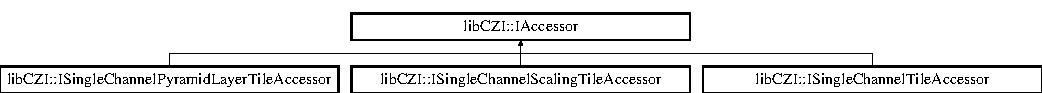
\includegraphics[height=1.252796cm]{classlib_c_z_i_1_1_i_accessor}
\end{center}
\end{figure}


\subsection{Detailed Description}
The base interface (all accessor-\/interface must derive from this). 

The documentation for this class was generated from the following file\+:\begin{DoxyCompactItemize}
\item 
lib\+C\+Z\+I/lib\+C\+Z\+I\+\_\+\+Compositor.\+h\end{DoxyCompactItemize}

\hypertarget{classlib_c_z_i_1_1_i_attachment}{}\section{lib\+C\+ZI\+:\+:I\+Attachment Class Reference}
\label{classlib_c_z_i_1_1_i_attachment}\index{lib\+C\+Z\+I\+::\+I\+Attachment@{lib\+C\+Z\+I\+::\+I\+Attachment}}


Representation of an attachment. An attachment is a binary blob, its inner structure is opaque.  




{\ttfamily \#include $<$lib\+C\+Z\+I.\+h$>$}

\subsection*{Public Member Functions}
\begin{DoxyCompactItemize}
\item 
virtual const \hyperlink{structlib_c_z_i_1_1_attachment_info}{Attachment\+Info} \& \hyperlink{classlib_c_z_i_1_1_i_attachment_adabcfe4e9a9198fca93445fe22a09c1c}{Get\+Attachment\+Info} () const =0
\item 
virtual void \hyperlink{classlib_c_z_i_1_1_i_attachment_ab809465974cfe7eaf10e171cc1c7bc15}{Dangerous\+Get\+Raw\+Data} (const void $\ast$\&ptr, size\+\_\+t \&size) const =0
\item 
virtual std\+::shared\+\_\+ptr$<$ const void $>$ \hyperlink{classlib_c_z_i_1_1_i_attachment_a123ae7b474e78b44cfbb3e36f2e74fd8}{Get\+Raw\+Data} (size\+\_\+t $\ast$ptr\+Size)=0
\item 
{\footnotesize template$<$class Q $>$ }\\void \hyperlink{classlib_c_z_i_1_1_i_attachment_a2f716dad937d9bc600c27ff33c94dd4e}{Dangerous\+Get\+Raw\+Data} (const Q $\ast$\&ptr, size\+\_\+t \&size) const
\end{DoxyCompactItemize}


\subsection{Detailed Description}
Representation of an attachment. An attachment is a binary blob, its inner structure is opaque. 

\subsection{Member Function Documentation}
\mbox{\Hypertarget{classlib_c_z_i_1_1_i_attachment_ab809465974cfe7eaf10e171cc1c7bc15}\label{classlib_c_z_i_1_1_i_attachment_ab809465974cfe7eaf10e171cc1c7bc15}} 
\index{lib\+C\+Z\+I\+::\+I\+Attachment@{lib\+C\+Z\+I\+::\+I\+Attachment}!Dangerous\+Get\+Raw\+Data@{Dangerous\+Get\+Raw\+Data}}
\index{Dangerous\+Get\+Raw\+Data@{Dangerous\+Get\+Raw\+Data}!lib\+C\+Z\+I\+::\+I\+Attachment@{lib\+C\+Z\+I\+::\+I\+Attachment}}
\subsubsection{\texorpdfstring{Dangerous\+Get\+Raw\+Data()}{DangerousGetRawData()}\hspace{0.1cm}{\footnotesize\ttfamily [1/2]}}
{\footnotesize\ttfamily virtual void lib\+C\+Z\+I\+::\+I\+Attachment\+::\+Dangerous\+Get\+Raw\+Data (\begin{DoxyParamCaption}\item[{const void $\ast$\&}]{ptr,  }\item[{size\+\_\+t \&}]{size }\end{DoxyParamCaption}) const\hspace{0.3cm}{\ttfamily [pure virtual]}}

Get a pointer to the raw data. Note that the pointer returned is only valid during the lifetime of the sub-\/block-\/object. 
\begin{DoxyParams}[1]{Parameters}
\mbox{\tt out}  & {\em ptr} & The pointer to the data is stored here. \\
\hline
\mbox{\tt out}  & {\em size} & The size of the data. \\
\hline
\end{DoxyParams}
\mbox{\Hypertarget{classlib_c_z_i_1_1_i_attachment_a2f716dad937d9bc600c27ff33c94dd4e}\label{classlib_c_z_i_1_1_i_attachment_a2f716dad937d9bc600c27ff33c94dd4e}} 
\index{lib\+C\+Z\+I\+::\+I\+Attachment@{lib\+C\+Z\+I\+::\+I\+Attachment}!Dangerous\+Get\+Raw\+Data@{Dangerous\+Get\+Raw\+Data}}
\index{Dangerous\+Get\+Raw\+Data@{Dangerous\+Get\+Raw\+Data}!lib\+C\+Z\+I\+::\+I\+Attachment@{lib\+C\+Z\+I\+::\+I\+Attachment}}
\subsubsection{\texorpdfstring{Dangerous\+Get\+Raw\+Data()}{DangerousGetRawData()}\hspace{0.1cm}{\footnotesize\ttfamily [2/2]}}
{\footnotesize\ttfamily template$<$class Q $>$ \\
void lib\+C\+Z\+I\+::\+I\+Attachment\+::\+Dangerous\+Get\+Raw\+Data (\begin{DoxyParamCaption}\item[{const Q $\ast$\&}]{ptr,  }\item[{size\+\_\+t \&}]{size }\end{DoxyParamCaption}) const\hspace{0.3cm}{\ttfamily [inline]}}

A helper method used to cast the pointer to a specific type. 
\begin{DoxyParams}[1]{Parameters}
\mbox{\tt out}  & {\em ptr} & The pointer to the data is stored here. \\
\hline
\mbox{\tt out}  & {\em size} & The size of the data. \\
\hline
\end{DoxyParams}
\mbox{\Hypertarget{classlib_c_z_i_1_1_i_attachment_adabcfe4e9a9198fca93445fe22a09c1c}\label{classlib_c_z_i_1_1_i_attachment_adabcfe4e9a9198fca93445fe22a09c1c}} 
\index{lib\+C\+Z\+I\+::\+I\+Attachment@{lib\+C\+Z\+I\+::\+I\+Attachment}!Get\+Attachment\+Info@{Get\+Attachment\+Info}}
\index{Get\+Attachment\+Info@{Get\+Attachment\+Info}!lib\+C\+Z\+I\+::\+I\+Attachment@{lib\+C\+Z\+I\+::\+I\+Attachment}}
\subsubsection{\texorpdfstring{Get\+Attachment\+Info()}{GetAttachmentInfo()}}
{\footnotesize\ttfamily virtual const \hyperlink{structlib_c_z_i_1_1_attachment_info}{Attachment\+Info}\& lib\+C\+Z\+I\+::\+I\+Attachment\+::\+Get\+Attachment\+Info (\begin{DoxyParamCaption}{ }\end{DoxyParamCaption}) const\hspace{0.3cm}{\ttfamily [pure virtual]}}

Gets information about the attachment. \begin{DoxyReturn}{Returns}
The attachment information. 
\end{DoxyReturn}
\mbox{\Hypertarget{classlib_c_z_i_1_1_i_attachment_a123ae7b474e78b44cfbb3e36f2e74fd8}\label{classlib_c_z_i_1_1_i_attachment_a123ae7b474e78b44cfbb3e36f2e74fd8}} 
\index{lib\+C\+Z\+I\+::\+I\+Attachment@{lib\+C\+Z\+I\+::\+I\+Attachment}!Get\+Raw\+Data@{Get\+Raw\+Data}}
\index{Get\+Raw\+Data@{Get\+Raw\+Data}!lib\+C\+Z\+I\+::\+I\+Attachment@{lib\+C\+Z\+I\+::\+I\+Attachment}}
\subsubsection{\texorpdfstring{Get\+Raw\+Data()}{GetRawData()}}
{\footnotesize\ttfamily virtual std\+::shared\+\_\+ptr$<$const void$>$ lib\+C\+Z\+I\+::\+I\+Attachment\+::\+Get\+Raw\+Data (\begin{DoxyParamCaption}\item[{size\+\_\+t $\ast$}]{ptr\+Size }\end{DoxyParamCaption})\hspace{0.3cm}{\ttfamily [pure virtual]}}

Gets raw data. 
\begin{DoxyParams}[1]{Parameters}
\mbox{\tt out}  & {\em ptr\+Size} & If non-\/null, size of the data buffer is stored here. \\
\hline
\end{DoxyParams}
\begin{DoxyReturn}{Returns}
The raw data. 
\end{DoxyReturn}


The documentation for this class was generated from the following file\+:\begin{DoxyCompactItemize}
\item 
lib\+C\+Z\+I/lib\+C\+Z\+I.\+h\end{DoxyCompactItemize}

\hypertarget{classlib_c_z_i_1_1_i_attachment_repository}{}\section{lib\+C\+ZI\+:\+:I\+Attachment\+Repository Class Reference}
\label{classlib_c_z_i_1_1_i_attachment_repository}\index{lib\+C\+Z\+I\+::\+I\+Attachment\+Repository@{lib\+C\+Z\+I\+::\+I\+Attachment\+Repository}}


Interface for the attachment repository. This interface is used to access the attachments in a C\+Z\+I-\/file.  




{\ttfamily \#include $<$lib\+C\+Z\+I.\+h$>$}

Inheritance diagram for lib\+C\+ZI\+:\+:I\+Attachment\+Repository\+:\begin{figure}[H]
\begin{center}
\leavevmode
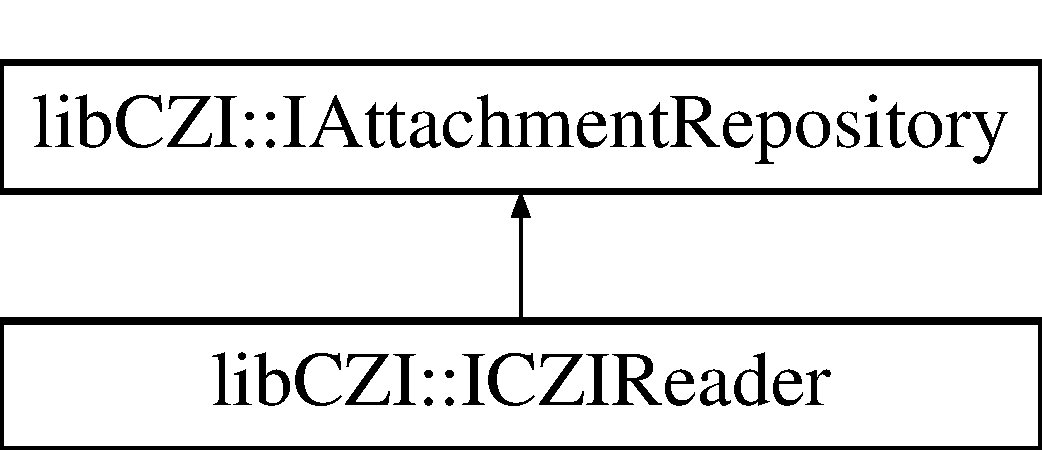
\includegraphics[height=2.000000cm]{classlib_c_z_i_1_1_i_attachment_repository}
\end{center}
\end{figure}
\subsection*{Public Member Functions}
\begin{DoxyCompactItemize}
\item 
virtual void \hyperlink{classlib_c_z_i_1_1_i_attachment_repository_a38f1c13a03e2dd8887d911be2c1b892b}{Enumerate\+Attachments} (std\+::function$<$ bool(int index, const \hyperlink{structlib_c_z_i_1_1_attachment_info}{Attachment\+Info} \&info)$>$ func\+Enum)=0
\item 
virtual void \hyperlink{classlib_c_z_i_1_1_i_attachment_repository_acc6b932d8d587bb8399c0236c1c29a55}{Enumerate\+Subset} (const char $\ast$content\+File\+Type, const char $\ast$name, std\+::function$<$ bool(int index, const \hyperlink{structlib_c_z_i_1_1_attachment_info}{Attachment\+Info} \&infi)$>$ func\+Enum)=0
\item 
virtual std\+::shared\+\_\+ptr$<$ \hyperlink{classlib_c_z_i_1_1_i_attachment}{I\+Attachment} $>$ \hyperlink{classlib_c_z_i_1_1_i_attachment_repository_a8f0a7a926425e39017559a95207e2d5d}{Read\+Attachment} (int index)=0
\end{DoxyCompactItemize}


\subsection{Detailed Description}
Interface for the attachment repository. This interface is used to access the attachments in a C\+Z\+I-\/file. 

\subsection{Member Function Documentation}
\mbox{\Hypertarget{classlib_c_z_i_1_1_i_attachment_repository_a38f1c13a03e2dd8887d911be2c1b892b}\label{classlib_c_z_i_1_1_i_attachment_repository_a38f1c13a03e2dd8887d911be2c1b892b}} 
\index{lib\+C\+Z\+I\+::\+I\+Attachment\+Repository@{lib\+C\+Z\+I\+::\+I\+Attachment\+Repository}!Enumerate\+Attachments@{Enumerate\+Attachments}}
\index{Enumerate\+Attachments@{Enumerate\+Attachments}!lib\+C\+Z\+I\+::\+I\+Attachment\+Repository@{lib\+C\+Z\+I\+::\+I\+Attachment\+Repository}}
\subsubsection{\texorpdfstring{Enumerate\+Attachments()}{EnumerateAttachments()}}
{\footnotesize\ttfamily virtual void lib\+C\+Z\+I\+::\+I\+Attachment\+Repository\+::\+Enumerate\+Attachments (\begin{DoxyParamCaption}\item[{std\+::function$<$ bool(int index, const \hyperlink{structlib_c_z_i_1_1_attachment_info}{Attachment\+Info} \&info)$>$}]{func\+Enum }\end{DoxyParamCaption})\hspace{0.3cm}{\ttfamily [pure virtual]}}

Enumerate all attachments.


\begin{DoxyParams}{Parameters}
{\em func\+Enum} & The functor which will be called for every attachment. If the return value of the functor is true, the enumeration is continued, otherwise it is stopped. The first argument is the index of the attachment and the second is providing information about the attachment. \\
\hline
\end{DoxyParams}
\mbox{\Hypertarget{classlib_c_z_i_1_1_i_attachment_repository_acc6b932d8d587bb8399c0236c1c29a55}\label{classlib_c_z_i_1_1_i_attachment_repository_acc6b932d8d587bb8399c0236c1c29a55}} 
\index{lib\+C\+Z\+I\+::\+I\+Attachment\+Repository@{lib\+C\+Z\+I\+::\+I\+Attachment\+Repository}!Enumerate\+Subset@{Enumerate\+Subset}}
\index{Enumerate\+Subset@{Enumerate\+Subset}!lib\+C\+Z\+I\+::\+I\+Attachment\+Repository@{lib\+C\+Z\+I\+::\+I\+Attachment\+Repository}}
\subsubsection{\texorpdfstring{Enumerate\+Subset()}{EnumerateSubset()}}
{\footnotesize\ttfamily virtual void lib\+C\+Z\+I\+::\+I\+Attachment\+Repository\+::\+Enumerate\+Subset (\begin{DoxyParamCaption}\item[{const char $\ast$}]{content\+File\+Type,  }\item[{const char $\ast$}]{name,  }\item[{std\+::function$<$ bool(int index, const \hyperlink{structlib_c_z_i_1_1_attachment_info}{Attachment\+Info} \&infi)$>$}]{func\+Enum }\end{DoxyParamCaption})\hspace{0.3cm}{\ttfamily [pure virtual]}}

Enumerate the subset of the attachments defined by the parameters. 
\begin{DoxyParams}{Parameters}
{\em content\+File\+Type} & If non-\/null, only attachments with this content\+File\+Type will be considered. \\
\hline
{\em name} & If non-\/null, only attachments with this name will be considered. \\
\hline
{\em func\+Enum} & The functor which will be called for every attachment (within the subset). If the return value of the functor is true, the enumeration is continued, otherwise it is stopped. The first argument is the index of the attachment and the second is providing information about the attachment. \\
\hline
\end{DoxyParams}
\mbox{\Hypertarget{classlib_c_z_i_1_1_i_attachment_repository_a8f0a7a926425e39017559a95207e2d5d}\label{classlib_c_z_i_1_1_i_attachment_repository_a8f0a7a926425e39017559a95207e2d5d}} 
\index{lib\+C\+Z\+I\+::\+I\+Attachment\+Repository@{lib\+C\+Z\+I\+::\+I\+Attachment\+Repository}!Read\+Attachment@{Read\+Attachment}}
\index{Read\+Attachment@{Read\+Attachment}!lib\+C\+Z\+I\+::\+I\+Attachment\+Repository@{lib\+C\+Z\+I\+::\+I\+Attachment\+Repository}}
\subsubsection{\texorpdfstring{Read\+Attachment()}{ReadAttachment()}}
{\footnotesize\ttfamily virtual std\+::shared\+\_\+ptr$<$\hyperlink{classlib_c_z_i_1_1_i_attachment}{I\+Attachment}$>$ lib\+C\+Z\+I\+::\+I\+Attachment\+Repository\+::\+Read\+Attachment (\begin{DoxyParamCaption}\item[{int}]{index }\end{DoxyParamCaption})\hspace{0.3cm}{\ttfamily [pure virtual]}}

Reads the attachment identified by the specified index. If there is no attachment present (for the specified index) then an empty shared\+\_\+ptr is returned. If a different kind of problem occurs (e. g. I/O error or corrupted data) an exception is thrown. 
\begin{DoxyParams}{Parameters}
{\em index} & Index of the attachment (as reported by the Enumerate-\/methods). \\
\hline
\end{DoxyParams}
\begin{DoxyReturn}{Returns}
If successful, the attachment object; otherwise an empty shared\+\_\+ptr. 
\end{DoxyReturn}


The documentation for this class was generated from the following file\+:\begin{DoxyCompactItemize}
\item 
lib\+C\+Z\+I/lib\+C\+Z\+I.\+h\end{DoxyCompactItemize}

\hypertarget{classlib_c_z_i_1_1_i_bitmap_data}{}\section{lib\+C\+ZI\+:\+:I\+Bitmap\+Data Class Reference}
\label{classlib_c_z_i_1_1_i_bitmap_data}\index{lib\+C\+Z\+I\+::\+I\+Bitmap\+Data@{lib\+C\+Z\+I\+::\+I\+Bitmap\+Data}}


{\ttfamily \#include $<$lib\+C\+Z\+I\+\_\+\+Pixels.\+h$>$}

\subsection*{Public Member Functions}
\begin{DoxyCompactItemize}
\item 
virtual \hyperlink{namespacelib_c_z_i_abf8ce12ab88b06c8b3b47efbb5e2e834}{Pixel\+Type} \hyperlink{classlib_c_z_i_1_1_i_bitmap_data_a66f27266674d7f328dd5f1270b81a94e}{Get\+Pixel\+Type} () const =0
\item 
virtual \hyperlink{structlib_c_z_i_1_1_int_size}{Int\+Size} \hyperlink{classlib_c_z_i_1_1_i_bitmap_data_af612716947147a55dcbbb245c3335ace}{Get\+Size} () const =0
\item 
virtual \hyperlink{structlib_c_z_i_1_1_bitmap_lock_info}{Bitmap\+Lock\+Info} \hyperlink{classlib_c_z_i_1_1_i_bitmap_data_afbdfc7266b37850cfb53d5106bfd4f44}{Lock} ()=0
\item 
virtual void \hyperlink{classlib_c_z_i_1_1_i_bitmap_data_a473c706c604fd687fb653bd06f0e0356}{Unlock} ()=0
\item 
std\+::uint32\+\_\+t \hyperlink{classlib_c_z_i_1_1_i_bitmap_data_aa2638991a88c736ff4e6c42dc4c6c5c7}{Get\+Width} () const
\item 
std\+::uint32\+\_\+t \hyperlink{classlib_c_z_i_1_1_i_bitmap_data_a2072b5c8db493b7b19717811a96a6483}{Get\+Height} () const
\end{DoxyCompactItemize}


\subsection{Detailed Description}
This interface is used to represent a bitmap.

In order to access the pixel data, the Lock-\/method must be called. The information returned from the Lock-\/method is to be considered valid only until Unlock is called. If a bitmap is destroyed while it is locked, this is considered to be a fatal error. It is legal to call Lock multiple times, but the calls to Lock and Unlock must be balanced. 

\subsection{Member Function Documentation}
\mbox{\Hypertarget{classlib_c_z_i_1_1_i_bitmap_data_a2072b5c8db493b7b19717811a96a6483}\label{classlib_c_z_i_1_1_i_bitmap_data_a2072b5c8db493b7b19717811a96a6483}} 
\index{lib\+C\+Z\+I\+::\+I\+Bitmap\+Data@{lib\+C\+Z\+I\+::\+I\+Bitmap\+Data}!Get\+Height@{Get\+Height}}
\index{Get\+Height@{Get\+Height}!lib\+C\+Z\+I\+::\+I\+Bitmap\+Data@{lib\+C\+Z\+I\+::\+I\+Bitmap\+Data}}
\subsubsection{\texorpdfstring{Get\+Height()}{GetHeight()}}
{\footnotesize\ttfamily std\+::uint32\+\_\+t lib\+C\+Z\+I\+::\+I\+Bitmap\+Data\+::\+Get\+Height (\begin{DoxyParamCaption}{ }\end{DoxyParamCaption}) const\hspace{0.3cm}{\ttfamily [inline]}}

Gets the height of the bitmap in pixels.

\begin{DoxyReturn}{Returns}
The height in pixels 
\end{DoxyReturn}
\mbox{\Hypertarget{classlib_c_z_i_1_1_i_bitmap_data_a66f27266674d7f328dd5f1270b81a94e}\label{classlib_c_z_i_1_1_i_bitmap_data_a66f27266674d7f328dd5f1270b81a94e}} 
\index{lib\+C\+Z\+I\+::\+I\+Bitmap\+Data@{lib\+C\+Z\+I\+::\+I\+Bitmap\+Data}!Get\+Pixel\+Type@{Get\+Pixel\+Type}}
\index{Get\+Pixel\+Type@{Get\+Pixel\+Type}!lib\+C\+Z\+I\+::\+I\+Bitmap\+Data@{lib\+C\+Z\+I\+::\+I\+Bitmap\+Data}}
\subsubsection{\texorpdfstring{Get\+Pixel\+Type()}{GetPixelType()}}
{\footnotesize\ttfamily virtual \hyperlink{namespacelib_c_z_i_abf8ce12ab88b06c8b3b47efbb5e2e834}{Pixel\+Type} lib\+C\+Z\+I\+::\+I\+Bitmap\+Data\+::\+Get\+Pixel\+Type (\begin{DoxyParamCaption}{ }\end{DoxyParamCaption}) const\hspace{0.3cm}{\ttfamily [pure virtual]}}

Gets pixel type.

\begin{DoxyReturn}{Returns}
The pixel type. 
\end{DoxyReturn}
\mbox{\Hypertarget{classlib_c_z_i_1_1_i_bitmap_data_af612716947147a55dcbbb245c3335ace}\label{classlib_c_z_i_1_1_i_bitmap_data_af612716947147a55dcbbb245c3335ace}} 
\index{lib\+C\+Z\+I\+::\+I\+Bitmap\+Data@{lib\+C\+Z\+I\+::\+I\+Bitmap\+Data}!Get\+Size@{Get\+Size}}
\index{Get\+Size@{Get\+Size}!lib\+C\+Z\+I\+::\+I\+Bitmap\+Data@{lib\+C\+Z\+I\+::\+I\+Bitmap\+Data}}
\subsubsection{\texorpdfstring{Get\+Size()}{GetSize()}}
{\footnotesize\ttfamily virtual \hyperlink{structlib_c_z_i_1_1_int_size}{Int\+Size} lib\+C\+Z\+I\+::\+I\+Bitmap\+Data\+::\+Get\+Size (\begin{DoxyParamCaption}{ }\end{DoxyParamCaption}) const\hspace{0.3cm}{\ttfamily [pure virtual]}}

Gets the size of the bitmap (i. e. its width and height in pixels).

\begin{DoxyReturn}{Returns}
The size (in pixels). 
\end{DoxyReturn}
\mbox{\Hypertarget{classlib_c_z_i_1_1_i_bitmap_data_aa2638991a88c736ff4e6c42dc4c6c5c7}\label{classlib_c_z_i_1_1_i_bitmap_data_aa2638991a88c736ff4e6c42dc4c6c5c7}} 
\index{lib\+C\+Z\+I\+::\+I\+Bitmap\+Data@{lib\+C\+Z\+I\+::\+I\+Bitmap\+Data}!Get\+Width@{Get\+Width}}
\index{Get\+Width@{Get\+Width}!lib\+C\+Z\+I\+::\+I\+Bitmap\+Data@{lib\+C\+Z\+I\+::\+I\+Bitmap\+Data}}
\subsubsection{\texorpdfstring{Get\+Width()}{GetWidth()}}
{\footnotesize\ttfamily std\+::uint32\+\_\+t lib\+C\+Z\+I\+::\+I\+Bitmap\+Data\+::\+Get\+Width (\begin{DoxyParamCaption}{ }\end{DoxyParamCaption}) const\hspace{0.3cm}{\ttfamily [inline]}}

Gets the width of the bitmap in pixels.

\begin{DoxyReturn}{Returns}
The width in pixels. 
\end{DoxyReturn}
\mbox{\Hypertarget{classlib_c_z_i_1_1_i_bitmap_data_afbdfc7266b37850cfb53d5106bfd4f44}\label{classlib_c_z_i_1_1_i_bitmap_data_afbdfc7266b37850cfb53d5106bfd4f44}} 
\index{lib\+C\+Z\+I\+::\+I\+Bitmap\+Data@{lib\+C\+Z\+I\+::\+I\+Bitmap\+Data}!Lock@{Lock}}
\index{Lock@{Lock}!lib\+C\+Z\+I\+::\+I\+Bitmap\+Data@{lib\+C\+Z\+I\+::\+I\+Bitmap\+Data}}
\subsubsection{\texorpdfstring{Lock()}{Lock()}}
{\footnotesize\ttfamily virtual \hyperlink{structlib_c_z_i_1_1_bitmap_lock_info}{Bitmap\+Lock\+Info} lib\+C\+Z\+I\+::\+I\+Bitmap\+Data\+::\+Lock (\begin{DoxyParamCaption}{ }\end{DoxyParamCaption})\hspace{0.3cm}{\ttfamily [pure virtual]}}

Gets a data structure allowing for direct access of the bitmap.

The \hyperlink{structlib_c_z_i_1_1_bitmap_lock_info}{Bitmap\+Lock\+Info} returned must only considered to be valid until Unlock is called. It is legal to call Lock multiple time (also from different threads concurrently). In any case, calls to Lock and Unlock must be balanced. It is considered to be a fatal error if the object is destroyed when it is locked.

\begin{DoxyReturn}{Returns}
The \hyperlink{structlib_c_z_i_1_1_bitmap_lock_info}{Bitmap\+Lock\+Info} allowing to directly access the data representing the bitmap. 
\end{DoxyReturn}
\mbox{\Hypertarget{classlib_c_z_i_1_1_i_bitmap_data_a473c706c604fd687fb653bd06f0e0356}\label{classlib_c_z_i_1_1_i_bitmap_data_a473c706c604fd687fb653bd06f0e0356}} 
\index{lib\+C\+Z\+I\+::\+I\+Bitmap\+Data@{lib\+C\+Z\+I\+::\+I\+Bitmap\+Data}!Unlock@{Unlock}}
\index{Unlock@{Unlock}!lib\+C\+Z\+I\+::\+I\+Bitmap\+Data@{lib\+C\+Z\+I\+::\+I\+Bitmap\+Data}}
\subsubsection{\texorpdfstring{Unlock()}{Unlock()}}
{\footnotesize\ttfamily virtual void lib\+C\+Z\+I\+::\+I\+Bitmap\+Data\+::\+Unlock (\begin{DoxyParamCaption}{ }\end{DoxyParamCaption})\hspace{0.3cm}{\ttfamily [pure virtual]}}

Inform the bitmap object that the data (previously retrieved by a call to Lock) is not longer used.

The \hyperlink{structlib_c_z_i_1_1_bitmap_lock_info}{Bitmap\+Lock\+Info} returned must only considered to be valid until Unlock is called. 

The documentation for this class was generated from the following file\+:\begin{DoxyCompactItemize}
\item 
lib\+C\+Z\+I/lib\+C\+Z\+I\+\_\+\+Pixels.\+h\end{DoxyCompactItemize}

\hypertarget{classlib_c_z_i_1_1_i_channel_display_setting}{}\section{lib\+C\+ZI\+:\+:I\+Channel\+Display\+Setting Class Reference}
\label{classlib_c_z_i_1_1_i_channel_display_setting}\index{lib\+C\+Z\+I\+::\+I\+Channel\+Display\+Setting@{lib\+C\+Z\+I\+::\+I\+Channel\+Display\+Setting}}


The display-\/settings for a channel.  




{\ttfamily \#include $<$lib\+C\+Z\+I\+\_\+\+Metadata.\+h$>$}

\subsection*{Public Member Functions}
\begin{DoxyCompactItemize}
\item 
virtual bool \hyperlink{classlib_c_z_i_1_1_i_channel_display_setting_a874cb106b686e6f4b7fad2f6dd1b3eed}{Get\+Is\+Enabled} () const =0
\item 
virtual float \hyperlink{classlib_c_z_i_1_1_i_channel_display_setting_ad4b5a8fed9cad0b28acbbfed7736a8d0}{Get\+Weight} () const =0
\item 
virtual bool \hyperlink{classlib_c_z_i_1_1_i_channel_display_setting_a7fd49b4a914738b4640eedef351cdd02}{Try\+Get\+Tinting\+Color\+Rgb8} (\hyperlink{structlib_c_z_i_1_1_rgb8_color}{lib\+C\+Z\+I\+::\+Rgb8\+Color} $\ast$p\+Color) const =0
\item 
virtual void \hyperlink{classlib_c_z_i_1_1_i_channel_display_setting_a1172fdc6f7c3131d5e6ddf6ab35c6f85}{Get\+Black\+White\+Point} (float $\ast$p\+Black, float $\ast$p\+White) const =0
\item 
virtual \hyperlink{classlib_c_z_i_1_1_i_display_settings_af114dfcc8a603ca1c2fc57bc35c97684}{I\+Display\+Settings\+::\+Gradation\+Curve\+Mode} \hyperlink{classlib_c_z_i_1_1_i_channel_display_setting_abcee850366caccfb3245c84ea6f71287}{Get\+Gradation\+Curve\+Mode} () const =0
\item 
virtual bool \hyperlink{classlib_c_z_i_1_1_i_channel_display_setting_a37a0c8e3159e6a5e3a9cd0c22b90fd2f}{Try\+Get\+Gamma} (float $\ast$gamma) const =0
\item 
virtual bool \hyperlink{classlib_c_z_i_1_1_i_channel_display_setting_ae8a2192fd92015fc6ce59958b598a8cb}{Try\+Get\+Spline\+Control\+Points} (std\+::vector$<$ \hyperlink{structlib_c_z_i_1_1_i_display_settings_1_1_spline_control_point}{lib\+C\+Z\+I\+::\+I\+Display\+Settings\+::\+Spline\+Control\+Point} $>$ $\ast$ctrl\+Pts) const =0
\item 
virtual bool \hyperlink{classlib_c_z_i_1_1_i_channel_display_setting_ae3779bf0fb5b48c8ee3549e2ebb3947f}{Try\+Get\+Spline\+Data} (std\+::vector$<$ \hyperlink{structlib_c_z_i_1_1_i_display_settings_1_1_spline_data}{lib\+C\+Z\+I\+::\+I\+Display\+Settings\+::\+Spline\+Data} $>$ $\ast$data) const =0
\end{DoxyCompactItemize}
\subsection*{Static Public Member Functions}
\begin{DoxyCompactItemize}
\item 
static void \hyperlink{classlib_c_z_i_1_1_i_channel_display_setting_ac7569b65161bdfbc2cc8841e2c9fc45d}{Clone} (const \hyperlink{classlib_c_z_i_1_1_i_channel_display_setting}{I\+Channel\+Display\+Setting} $\ast$disp, \hyperlink{structlib_c_z_i_1_1_channel_display_settings_p_o_d}{Channel\+Display\+Settings\+P\+OD} \&pod)
\end{DoxyCompactItemize}


\subsection{Detailed Description}
The display-\/settings for a channel. 

\subsection{Member Function Documentation}
\mbox{\Hypertarget{classlib_c_z_i_1_1_i_channel_display_setting_ac7569b65161bdfbc2cc8841e2c9fc45d}\label{classlib_c_z_i_1_1_i_channel_display_setting_ac7569b65161bdfbc2cc8841e2c9fc45d}} 
\index{lib\+C\+Z\+I\+::\+I\+Channel\+Display\+Setting@{lib\+C\+Z\+I\+::\+I\+Channel\+Display\+Setting}!Clone@{Clone}}
\index{Clone@{Clone}!lib\+C\+Z\+I\+::\+I\+Channel\+Display\+Setting@{lib\+C\+Z\+I\+::\+I\+Channel\+Display\+Setting}}
\subsubsection{\texorpdfstring{Clone()}{Clone()}}
{\footnotesize\ttfamily static void lib\+C\+Z\+I\+::\+I\+Channel\+Display\+Setting\+::\+Clone (\begin{DoxyParamCaption}\item[{const \hyperlink{classlib_c_z_i_1_1_i_channel_display_setting}{I\+Channel\+Display\+Setting} $\ast$}]{disp,  }\item[{\hyperlink{structlib_c_z_i_1_1_channel_display_settings_p_o_d}{Channel\+Display\+Settings\+P\+OD} \&}]{pod }\end{DoxyParamCaption})\hspace{0.3cm}{\ttfamily [static]}}

Makes a deep copy of the information in this object and store the information in the P\+OD. 
\begin{DoxyParams}[1]{Parameters}
 & {\em disp} & The channel-\/display-\/settings object. \\
\hline
\mbox{\tt in,out}  & {\em pod} & The P\+O\+D-\/channel-\/display-\/settings object to store the information in. \\
\hline
\end{DoxyParams}
\mbox{\Hypertarget{classlib_c_z_i_1_1_i_channel_display_setting_a1172fdc6f7c3131d5e6ddf6ab35c6f85}\label{classlib_c_z_i_1_1_i_channel_display_setting_a1172fdc6f7c3131d5e6ddf6ab35c6f85}} 
\index{lib\+C\+Z\+I\+::\+I\+Channel\+Display\+Setting@{lib\+C\+Z\+I\+::\+I\+Channel\+Display\+Setting}!Get\+Black\+White\+Point@{Get\+Black\+White\+Point}}
\index{Get\+Black\+White\+Point@{Get\+Black\+White\+Point}!lib\+C\+Z\+I\+::\+I\+Channel\+Display\+Setting@{lib\+C\+Z\+I\+::\+I\+Channel\+Display\+Setting}}
\subsubsection{\texorpdfstring{Get\+Black\+White\+Point()}{GetBlackWhitePoint()}}
{\footnotesize\ttfamily virtual void lib\+C\+Z\+I\+::\+I\+Channel\+Display\+Setting\+::\+Get\+Black\+White\+Point (\begin{DoxyParamCaption}\item[{float $\ast$}]{p\+Black,  }\item[{float $\ast$}]{p\+White }\end{DoxyParamCaption}) const\hspace{0.3cm}{\ttfamily [pure virtual]}}

Gets the black point and the white point.


\begin{DoxyParams}[1]{Parameters}
\mbox{\tt out}  & {\em p\+Black} & If non-\/null, the black point will be returned. \\
\hline
\mbox{\tt out}  & {\em p\+White} & If non-\/null, the white point will be returned. \\
\hline
\end{DoxyParams}
\mbox{\Hypertarget{classlib_c_z_i_1_1_i_channel_display_setting_abcee850366caccfb3245c84ea6f71287}\label{classlib_c_z_i_1_1_i_channel_display_setting_abcee850366caccfb3245c84ea6f71287}} 
\index{lib\+C\+Z\+I\+::\+I\+Channel\+Display\+Setting@{lib\+C\+Z\+I\+::\+I\+Channel\+Display\+Setting}!Get\+Gradation\+Curve\+Mode@{Get\+Gradation\+Curve\+Mode}}
\index{Get\+Gradation\+Curve\+Mode@{Get\+Gradation\+Curve\+Mode}!lib\+C\+Z\+I\+::\+I\+Channel\+Display\+Setting@{lib\+C\+Z\+I\+::\+I\+Channel\+Display\+Setting}}
\subsubsection{\texorpdfstring{Get\+Gradation\+Curve\+Mode()}{GetGradationCurveMode()}}
{\footnotesize\ttfamily virtual \hyperlink{classlib_c_z_i_1_1_i_display_settings_af114dfcc8a603ca1c2fc57bc35c97684}{I\+Display\+Settings\+::\+Gradation\+Curve\+Mode} lib\+C\+Z\+I\+::\+I\+Channel\+Display\+Setting\+::\+Get\+Gradation\+Curve\+Mode (\begin{DoxyParamCaption}{ }\end{DoxyParamCaption}) const\hspace{0.3cm}{\ttfamily [pure virtual]}}

Gets gradation curve mode.

\begin{DoxyReturn}{Returns}
The gradation curve mode. 
\end{DoxyReturn}
\mbox{\Hypertarget{classlib_c_z_i_1_1_i_channel_display_setting_a874cb106b686e6f4b7fad2f6dd1b3eed}\label{classlib_c_z_i_1_1_i_channel_display_setting_a874cb106b686e6f4b7fad2f6dd1b3eed}} 
\index{lib\+C\+Z\+I\+::\+I\+Channel\+Display\+Setting@{lib\+C\+Z\+I\+::\+I\+Channel\+Display\+Setting}!Get\+Is\+Enabled@{Get\+Is\+Enabled}}
\index{Get\+Is\+Enabled@{Get\+Is\+Enabled}!lib\+C\+Z\+I\+::\+I\+Channel\+Display\+Setting@{lib\+C\+Z\+I\+::\+I\+Channel\+Display\+Setting}}
\subsubsection{\texorpdfstring{Get\+Is\+Enabled()}{GetIsEnabled()}}
{\footnotesize\ttfamily virtual bool lib\+C\+Z\+I\+::\+I\+Channel\+Display\+Setting\+::\+Get\+Is\+Enabled (\begin{DoxyParamCaption}{ }\end{DoxyParamCaption}) const\hspace{0.3cm}{\ttfamily [pure virtual]}}

Gets a boolean indicating whether the corresponding channel is \textquotesingle{}active\textquotesingle{} in the multi-\/channel-\/composition.

\begin{DoxyReturn}{Returns}
True if the corresponding channel is \textquotesingle{}active\textquotesingle{}, false otherwise. 
\end{DoxyReturn}
\mbox{\Hypertarget{classlib_c_z_i_1_1_i_channel_display_setting_ad4b5a8fed9cad0b28acbbfed7736a8d0}\label{classlib_c_z_i_1_1_i_channel_display_setting_ad4b5a8fed9cad0b28acbbfed7736a8d0}} 
\index{lib\+C\+Z\+I\+::\+I\+Channel\+Display\+Setting@{lib\+C\+Z\+I\+::\+I\+Channel\+Display\+Setting}!Get\+Weight@{Get\+Weight}}
\index{Get\+Weight@{Get\+Weight}!lib\+C\+Z\+I\+::\+I\+Channel\+Display\+Setting@{lib\+C\+Z\+I\+::\+I\+Channel\+Display\+Setting}}
\subsubsection{\texorpdfstring{Get\+Weight()}{GetWeight()}}
{\footnotesize\ttfamily virtual float lib\+C\+Z\+I\+::\+I\+Channel\+Display\+Setting\+::\+Get\+Weight (\begin{DoxyParamCaption}{ }\end{DoxyParamCaption}) const\hspace{0.3cm}{\ttfamily [pure virtual]}}

Gets the weight of the channel (for multi-\/channel-\/composition).

\begin{DoxyReturn}{Returns}
The weight. 
\end{DoxyReturn}
\mbox{\Hypertarget{classlib_c_z_i_1_1_i_channel_display_setting_a37a0c8e3159e6a5e3a9cd0c22b90fd2f}\label{classlib_c_z_i_1_1_i_channel_display_setting_a37a0c8e3159e6a5e3a9cd0c22b90fd2f}} 
\index{lib\+C\+Z\+I\+::\+I\+Channel\+Display\+Setting@{lib\+C\+Z\+I\+::\+I\+Channel\+Display\+Setting}!Try\+Get\+Gamma@{Try\+Get\+Gamma}}
\index{Try\+Get\+Gamma@{Try\+Get\+Gamma}!lib\+C\+Z\+I\+::\+I\+Channel\+Display\+Setting@{lib\+C\+Z\+I\+::\+I\+Channel\+Display\+Setting}}
\subsubsection{\texorpdfstring{Try\+Get\+Gamma()}{TryGetGamma()}}
{\footnotesize\ttfamily virtual bool lib\+C\+Z\+I\+::\+I\+Channel\+Display\+Setting\+::\+Try\+Get\+Gamma (\begin{DoxyParamCaption}\item[{float $\ast$}]{gamma }\end{DoxyParamCaption}) const\hspace{0.3cm}{\ttfamily [pure virtual]}}

Attempts to get the gamma -\/ this will only be available if gradation curve mode is {\ttfamily Gamma}.


\begin{DoxyParams}[1]{Parameters}
\mbox{\tt out}  & {\em gamma} & If non-\/null and applicable, the gamma will be returned.\\
\hline
\end{DoxyParams}
\begin{DoxyReturn}{Returns}
True if the corresponding channel uses gradation curve mode {\ttfamily Gamma} (and a value for gamma is available), false otherwise. 
\end{DoxyReturn}
\mbox{\Hypertarget{classlib_c_z_i_1_1_i_channel_display_setting_ae8a2192fd92015fc6ce59958b598a8cb}\label{classlib_c_z_i_1_1_i_channel_display_setting_ae8a2192fd92015fc6ce59958b598a8cb}} 
\index{lib\+C\+Z\+I\+::\+I\+Channel\+Display\+Setting@{lib\+C\+Z\+I\+::\+I\+Channel\+Display\+Setting}!Try\+Get\+Spline\+Control\+Points@{Try\+Get\+Spline\+Control\+Points}}
\index{Try\+Get\+Spline\+Control\+Points@{Try\+Get\+Spline\+Control\+Points}!lib\+C\+Z\+I\+::\+I\+Channel\+Display\+Setting@{lib\+C\+Z\+I\+::\+I\+Channel\+Display\+Setting}}
\subsubsection{\texorpdfstring{Try\+Get\+Spline\+Control\+Points()}{TryGetSplineControlPoints()}}
{\footnotesize\ttfamily virtual bool lib\+C\+Z\+I\+::\+I\+Channel\+Display\+Setting\+::\+Try\+Get\+Spline\+Control\+Points (\begin{DoxyParamCaption}\item[{std\+::vector$<$ \hyperlink{structlib_c_z_i_1_1_i_display_settings_1_1_spline_control_point}{lib\+C\+Z\+I\+::\+I\+Display\+Settings\+::\+Spline\+Control\+Point} $>$ $\ast$}]{ctrl\+Pts }\end{DoxyParamCaption}) const\hspace{0.3cm}{\ttfamily [pure virtual]}}

Attempts to get spline control points -\/ this will only be available if gradation curve mode is {\ttfamily Spline}. \begin{DoxyRemark}{Remarks}
We make no promises that both the control-\/points and the spline-\/data are always available. It might be plausible that the spline is defined in a different way (different than control-\/points), so in that case only the \char`\"{}spline-\/data\char`\"{} would be available. So -\/ be careful is using this interface in a context different thant \char`\"{}\+C\+Z\+I-\/metadata\char`\"{} where it might be the case the \textquotesingle{}Try\+Get\+Spline\+Control\+Points\textquotesingle{} will fail but \textquotesingle{}Try\+Get\+Spline\+Data\textquotesingle{} might succeed. Maybe better should remove \textquotesingle{}Try\+Get\+Spline\+Data\textquotesingle{} from this interface.
\end{DoxyRemark}

\begin{DoxyParams}[1]{Parameters}
\mbox{\tt in,out}  & {\em ctrl\+Pts} & If non-\/null, the control points will be written to this vector.\\
\hline
\end{DoxyParams}
\begin{DoxyReturn}{Returns}
True if it succeeds, false if it fails. 
\end{DoxyReturn}
\mbox{\Hypertarget{classlib_c_z_i_1_1_i_channel_display_setting_ae3779bf0fb5b48c8ee3549e2ebb3947f}\label{classlib_c_z_i_1_1_i_channel_display_setting_ae3779bf0fb5b48c8ee3549e2ebb3947f}} 
\index{lib\+C\+Z\+I\+::\+I\+Channel\+Display\+Setting@{lib\+C\+Z\+I\+::\+I\+Channel\+Display\+Setting}!Try\+Get\+Spline\+Data@{Try\+Get\+Spline\+Data}}
\index{Try\+Get\+Spline\+Data@{Try\+Get\+Spline\+Data}!lib\+C\+Z\+I\+::\+I\+Channel\+Display\+Setting@{lib\+C\+Z\+I\+::\+I\+Channel\+Display\+Setting}}
\subsubsection{\texorpdfstring{Try\+Get\+Spline\+Data()}{TryGetSplineData()}}
{\footnotesize\ttfamily virtual bool lib\+C\+Z\+I\+::\+I\+Channel\+Display\+Setting\+::\+Try\+Get\+Spline\+Data (\begin{DoxyParamCaption}\item[{std\+::vector$<$ \hyperlink{structlib_c_z_i_1_1_i_display_settings_1_1_spline_data}{lib\+C\+Z\+I\+::\+I\+Display\+Settings\+::\+Spline\+Data} $>$ $\ast$}]{data }\end{DoxyParamCaption}) const\hspace{0.3cm}{\ttfamily [pure virtual]}}

Attempts to get the spline data -\/ this will only be available if gradation curve mode is {\ttfamily Spline}.


\begin{DoxyParams}[1]{Parameters}
\mbox{\tt in,out}  & {\em data} & If non-\/null, the spline data will be written to this vector.\\
\hline
\end{DoxyParams}
\begin{DoxyReturn}{Returns}
True if it the corresponding channels uses gradation curve mode {\ttfamily Spline}, false otherwise. 
\end{DoxyReturn}
\mbox{\Hypertarget{classlib_c_z_i_1_1_i_channel_display_setting_a7fd49b4a914738b4640eedef351cdd02}\label{classlib_c_z_i_1_1_i_channel_display_setting_a7fd49b4a914738b4640eedef351cdd02}} 
\index{lib\+C\+Z\+I\+::\+I\+Channel\+Display\+Setting@{lib\+C\+Z\+I\+::\+I\+Channel\+Display\+Setting}!Try\+Get\+Tinting\+Color\+Rgb8@{Try\+Get\+Tinting\+Color\+Rgb8}}
\index{Try\+Get\+Tinting\+Color\+Rgb8@{Try\+Get\+Tinting\+Color\+Rgb8}!lib\+C\+Z\+I\+::\+I\+Channel\+Display\+Setting@{lib\+C\+Z\+I\+::\+I\+Channel\+Display\+Setting}}
\subsubsection{\texorpdfstring{Try\+Get\+Tinting\+Color\+Rgb8()}{TryGetTintingColorRgb8()}}
{\footnotesize\ttfamily virtual bool lib\+C\+Z\+I\+::\+I\+Channel\+Display\+Setting\+::\+Try\+Get\+Tinting\+Color\+Rgb8 (\begin{DoxyParamCaption}\item[{\hyperlink{structlib_c_z_i_1_1_rgb8_color}{lib\+C\+Z\+I\+::\+Rgb8\+Color} $\ast$}]{p\+Color }\end{DoxyParamCaption}) const\hspace{0.3cm}{\ttfamily [pure virtual]}}

Attempts to get the R\+G\+B24-\/tinting color for the corresponding channel. If tinting is not enabled, then this method will return false.


\begin{DoxyParams}[1]{Parameters}
\mbox{\tt out}  & {\em p\+Color} & If tinting is enabled for the corresponding channel, then (if non-\/null) will receive the tinting-\/color.\\
\hline
\end{DoxyParams}
\begin{DoxyReturn}{Returns}
True if tinting is enabled for the corresponding channel (and in this case {\ttfamily p\+Color} will be set), false otherwise (and {\ttfamily p\+Color} will not be set). 
\end{DoxyReturn}


The documentation for this class was generated from the following file\+:\begin{DoxyCompactItemize}
\item 
lib\+C\+Z\+I/lib\+C\+Z\+I\+\_\+\+Metadata.\+h\end{DoxyCompactItemize}

\hypertarget{classlib_c_z_i_1_1_i_czi_metadata}{}\section{lib\+C\+ZI\+:\+:I\+Czi\+Metadata Class Reference}
\label{classlib_c_z_i_1_1_i_czi_metadata}\index{lib\+C\+Z\+I\+::\+I\+Czi\+Metadata@{lib\+C\+Z\+I\+::\+I\+Czi\+Metadata}}


Representation of the C\+Z\+I-\/metadata.  




{\ttfamily \#include $<$lib\+C\+Z\+I\+\_\+\+Metadata.\+h$>$}

Inheritance diagram for lib\+C\+ZI\+:\+:I\+Czi\+Metadata\+:\begin{figure}[H]
\begin{center}
\leavevmode
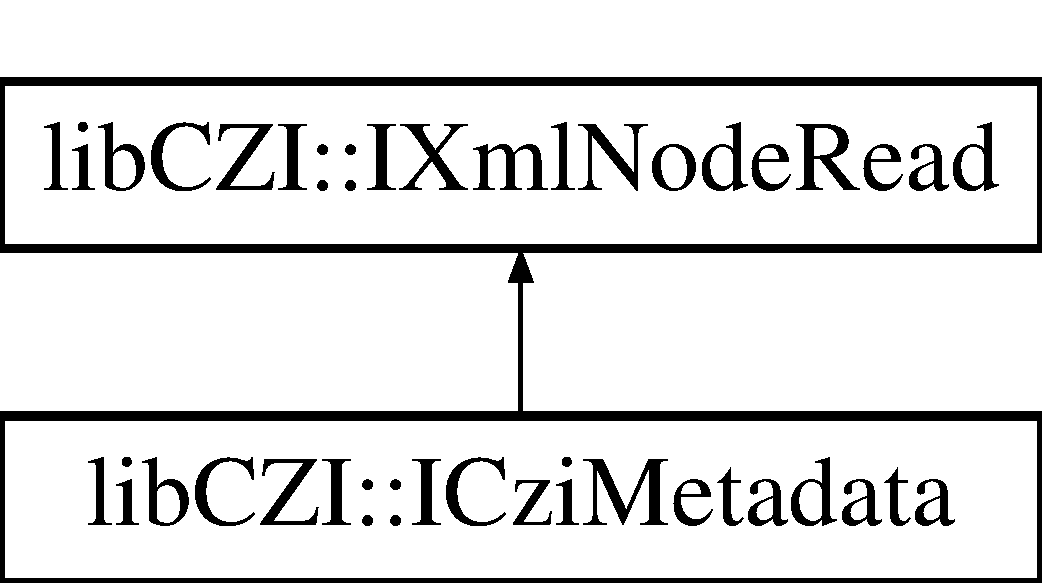
\includegraphics[height=2.000000cm]{classlib_c_z_i_1_1_i_czi_metadata}
\end{center}
\end{figure}
\subsection*{Public Member Functions}
\begin{DoxyCompactItemize}
\item 
virtual bool \hyperlink{classlib_c_z_i_1_1_i_czi_metadata_aa0465981ea6ea4d2165c7dd20e4b6833}{Is\+Xml\+Valid} () const =0
\item 
virtual std\+::string \hyperlink{classlib_c_z_i_1_1_i_czi_metadata_afd73a12ac5a04a725ad9f3d130f4e2de}{Get\+Xml} ()=0
\item 
virtual std\+::shared\+\_\+ptr$<$ \hyperlink{classlib_c_z_i_1_1_i_czi_multi_dimension_document_info}{lib\+C\+Z\+I\+::\+I\+Czi\+Multi\+Dimension\+Document\+Info} $>$ \hyperlink{classlib_c_z_i_1_1_i_czi_metadata_adf1a44d893d1f1aac6639bc39edda5af}{Get\+Document\+Info} ()=0
\end{DoxyCompactItemize}


\subsection{Detailed Description}
Representation of the C\+Z\+I-\/metadata. 

\subsection{Member Function Documentation}
\mbox{\Hypertarget{classlib_c_z_i_1_1_i_czi_metadata_adf1a44d893d1f1aac6639bc39edda5af}\label{classlib_c_z_i_1_1_i_czi_metadata_adf1a44d893d1f1aac6639bc39edda5af}} 
\index{lib\+C\+Z\+I\+::\+I\+Czi\+Metadata@{lib\+C\+Z\+I\+::\+I\+Czi\+Metadata}!Get\+Document\+Info@{Get\+Document\+Info}}
\index{Get\+Document\+Info@{Get\+Document\+Info}!lib\+C\+Z\+I\+::\+I\+Czi\+Metadata@{lib\+C\+Z\+I\+::\+I\+Czi\+Metadata}}
\subsubsection{\texorpdfstring{Get\+Document\+Info()}{GetDocumentInfo()}}
{\footnotesize\ttfamily virtual std\+::shared\+\_\+ptr$<$\hyperlink{classlib_c_z_i_1_1_i_czi_multi_dimension_document_info}{lib\+C\+Z\+I\+::\+I\+Czi\+Multi\+Dimension\+Document\+Info}$>$ lib\+C\+Z\+I\+::\+I\+Czi\+Metadata\+::\+Get\+Document\+Info (\begin{DoxyParamCaption}{ }\end{DoxyParamCaption})\hspace{0.3cm}{\ttfamily [pure virtual]}}

Gets the \char`\"{}document information\char`\"{} part of the metadata.

\begin{DoxyReturn}{Returns}
The \char`\"{}document information\char`\"{}. 
\end{DoxyReturn}
\mbox{\Hypertarget{classlib_c_z_i_1_1_i_czi_metadata_afd73a12ac5a04a725ad9f3d130f4e2de}\label{classlib_c_z_i_1_1_i_czi_metadata_afd73a12ac5a04a725ad9f3d130f4e2de}} 
\index{lib\+C\+Z\+I\+::\+I\+Czi\+Metadata@{lib\+C\+Z\+I\+::\+I\+Czi\+Metadata}!Get\+Xml@{Get\+Xml}}
\index{Get\+Xml@{Get\+Xml}!lib\+C\+Z\+I\+::\+I\+Czi\+Metadata@{lib\+C\+Z\+I\+::\+I\+Czi\+Metadata}}
\subsubsection{\texorpdfstring{Get\+Xml()}{GetXml()}}
{\footnotesize\ttfamily virtual std\+::string lib\+C\+Z\+I\+::\+I\+Czi\+Metadata\+::\+Get\+Xml (\begin{DoxyParamCaption}{ }\end{DoxyParamCaption})\hspace{0.3cm}{\ttfamily [pure virtual]}}

Gets the metadata as an unprocessed U\+T\+F8-\/encoded X\+M\+L-\/string.

\begin{DoxyReturn}{Returns}
The metadata (unprocessed U\+T\+F8-\/encoded X\+ML). 
\end{DoxyReturn}
\mbox{\Hypertarget{classlib_c_z_i_1_1_i_czi_metadata_aa0465981ea6ea4d2165c7dd20e4b6833}\label{classlib_c_z_i_1_1_i_czi_metadata_aa0465981ea6ea4d2165c7dd20e4b6833}} 
\index{lib\+C\+Z\+I\+::\+I\+Czi\+Metadata@{lib\+C\+Z\+I\+::\+I\+Czi\+Metadata}!Is\+Xml\+Valid@{Is\+Xml\+Valid}}
\index{Is\+Xml\+Valid@{Is\+Xml\+Valid}!lib\+C\+Z\+I\+::\+I\+Czi\+Metadata@{lib\+C\+Z\+I\+::\+I\+Czi\+Metadata}}
\subsubsection{\texorpdfstring{Is\+Xml\+Valid()}{IsXmlValid()}}
{\footnotesize\ttfamily virtual bool lib\+C\+Z\+I\+::\+I\+Czi\+Metadata\+::\+Is\+Xml\+Valid (\begin{DoxyParamCaption}{ }\end{DoxyParamCaption}) const\hspace{0.3cm}{\ttfamily [pure virtual]}}

Query if the C\+ZI\textquotesingle{}s metadata (the X\+ML) is well-\/formed and parsed correctly. If this is not the case, then other methods (of this interface) will thrown a \hyperlink{classlib_c_z_i_1_1_lib_c_z_i_xml_parse_exception}{Lib\+C\+Z\+I\+Xml\+Parse\+Exception} exception.

\begin{DoxyReturn}{Returns}
True if the X\+ML is well-\/formed, false if not. 
\end{DoxyReturn}


The documentation for this class was generated from the following file\+:\begin{DoxyCompactItemize}
\item 
lib\+C\+Z\+I/lib\+C\+Z\+I\+\_\+\+Metadata.\+h\end{DoxyCompactItemize}

\hypertarget{classlib_c_z_i_1_1_i_czi_multi_dimension_document_info}{}\section{lib\+C\+ZI\+:\+:I\+Czi\+Multi\+Dimension\+Document\+Info Class Reference}
\label{classlib_c_z_i_1_1_i_czi_multi_dimension_document_info}\index{lib\+C\+Z\+I\+::\+I\+Czi\+Multi\+Dimension\+Document\+Info@{lib\+C\+Z\+I\+::\+I\+Czi\+Multi\+Dimension\+Document\+Info}}


The top-\/level interface for the C\+Z\+I-\/metadata object.  




{\ttfamily \#include $<$lib\+C\+Z\+I\+\_\+\+Metadata.\+h$>$}

\subsection*{Public Member Functions}
\begin{DoxyCompactItemize}
\item 
virtual \hyperlink{structlib_c_z_i_1_1_general_document_info}{General\+Document\+Info} \hyperlink{classlib_c_z_i_1_1_i_czi_multi_dimension_document_info_aefea877fc65e9510d9a3127e366cb85c}{Get\+General\+Document\+Info} () const =0
\item 
virtual \hyperlink{structlib_c_z_i_1_1_scaling_info_ex}{lib\+C\+Z\+I\+::\+Scaling\+Info\+Ex} \hyperlink{classlib_c_z_i_1_1_i_czi_multi_dimension_document_info_a78275ba9453cb6a75081079d0a5bac1c}{Get\+Scaling\+Info\+Ex} () const =0
\item 
virtual \hyperlink{structlib_c_z_i_1_1_scaling_info}{lib\+C\+Z\+I\+::\+Scaling\+Info} \hyperlink{classlib_c_z_i_1_1_i_czi_multi_dimension_document_info_ae94341e3e5824b8c1d5c84928ced2e6c}{Get\+Scaling\+Info} () const =0
\item 
virtual void \hyperlink{classlib_c_z_i_1_1_i_czi_multi_dimension_document_info_a23f7b26bd323732fac0d190e9b38b6e3}{Enum\+Dimensions} (std\+::function$<$ bool(\hyperlink{namespacelib_c_z_i_a55049658acf59d0eddfaebcad16df424}{Dimension\+Index})$>$ enum\+Dimensions)=0
\item 
virtual std\+::shared\+\_\+ptr$<$ \hyperlink{classlib_c_z_i_1_1_i_dimension_info}{I\+Dimension\+Info} $>$ \hyperlink{classlib_c_z_i_1_1_i_czi_multi_dimension_document_info_a1e5d72c39dc22f99e1ee27b21055d3ea}{Get\+Dimension\+Info} (\hyperlink{namespacelib_c_z_i_a55049658acf59d0eddfaebcad16df424}{Dimension\+Index} dim)=0
\item 
virtual std\+::shared\+\_\+ptr$<$ \hyperlink{classlib_c_z_i_1_1_i_dimension_z_info}{I\+Dimension\+Z\+Info} $>$ \hyperlink{classlib_c_z_i_1_1_i_czi_multi_dimension_document_info_a58fbba886729ac71ae4be8a75a6e96f5}{Get\+Dimension\+Z\+Info} ()=0
\item 
virtual std\+::shared\+\_\+ptr$<$ \hyperlink{classlib_c_z_i_1_1_i_dimension_t_info}{I\+Dimension\+T\+Info} $>$ \hyperlink{classlib_c_z_i_1_1_i_czi_multi_dimension_document_info_a5b052b9eaa3b4e2dadb7ffe6e222006c}{Get\+Dimension\+T\+Info} ()=0
\item 
\mbox{\Hypertarget{classlib_c_z_i_1_1_i_czi_multi_dimension_document_info_a8ae66d4d866ddd93efd19b1cb0d54b0e}\label{classlib_c_z_i_1_1_i_czi_multi_dimension_document_info_a8ae66d4d866ddd93efd19b1cb0d54b0e}} 
virtual std\+::shared\+\_\+ptr$<$ I\+Dimensions\+Channels\+Info $>$ {\bfseries Get\+Dimension\+Channels\+Info} ()=0
\item 
virtual std\+::shared\+\_\+ptr$<$ \hyperlink{classlib_c_z_i_1_1_i_display_settings}{I\+Display\+Settings} $>$ \hyperlink{classlib_c_z_i_1_1_i_czi_multi_dimension_document_info_a8aff8239a31b047b737f80be0b2c9bda}{Get\+Display\+Settings} () const =0
\item 
std\+::vector$<$ \hyperlink{namespacelib_c_z_i_a55049658acf59d0eddfaebcad16df424}{Dimension\+Index} $>$ \hyperlink{classlib_c_z_i_1_1_i_czi_multi_dimension_document_info_aede2d6dd6e991151afff77b0cb96834a}{Get\+Dimensions} ()
\end{DoxyCompactItemize}


\subsection{Detailed Description}
The top-\/level interface for the C\+Z\+I-\/metadata object. 

\subsection{Member Function Documentation}
\mbox{\Hypertarget{classlib_c_z_i_1_1_i_czi_multi_dimension_document_info_a23f7b26bd323732fac0d190e9b38b6e3}\label{classlib_c_z_i_1_1_i_czi_multi_dimension_document_info_a23f7b26bd323732fac0d190e9b38b6e3}} 
\index{lib\+C\+Z\+I\+::\+I\+Czi\+Multi\+Dimension\+Document\+Info@{lib\+C\+Z\+I\+::\+I\+Czi\+Multi\+Dimension\+Document\+Info}!Enum\+Dimensions@{Enum\+Dimensions}}
\index{Enum\+Dimensions@{Enum\+Dimensions}!lib\+C\+Z\+I\+::\+I\+Czi\+Multi\+Dimension\+Document\+Info@{lib\+C\+Z\+I\+::\+I\+Czi\+Multi\+Dimension\+Document\+Info}}
\subsubsection{\texorpdfstring{Enum\+Dimensions()}{EnumDimensions()}}
{\footnotesize\ttfamily virtual void lib\+C\+Z\+I\+::\+I\+Czi\+Multi\+Dimension\+Document\+Info\+::\+Enum\+Dimensions (\begin{DoxyParamCaption}\item[{std\+::function$<$ bool(\hyperlink{namespacelib_c_z_i_a55049658acf59d0eddfaebcad16df424}{Dimension\+Index})$>$}]{enum\+Dimensions }\end{DoxyParamCaption})\hspace{0.3cm}{\ttfamily [pure virtual]}}

Enumerate the dimensions (defined in the metadata under Metadata/\+Information/\+Image, checking for the nodes StartZ, SizeZ, StartC, SizeC, StartT, StartT, ...). \begin{DoxyRemark}{Remarks}
The information here is not considered authoritative. 
\end{DoxyRemark}

\begin{DoxyParams}{Parameters}
{\em enum\+Dimensions} & The functor which will be called for each dimension. If the functor returns false, the enumeration is canceled. \\
\hline
\end{DoxyParams}
\mbox{\Hypertarget{classlib_c_z_i_1_1_i_czi_multi_dimension_document_info_a1e5d72c39dc22f99e1ee27b21055d3ea}\label{classlib_c_z_i_1_1_i_czi_multi_dimension_document_info_a1e5d72c39dc22f99e1ee27b21055d3ea}} 
\index{lib\+C\+Z\+I\+::\+I\+Czi\+Multi\+Dimension\+Document\+Info@{lib\+C\+Z\+I\+::\+I\+Czi\+Multi\+Dimension\+Document\+Info}!Get\+Dimension\+Info@{Get\+Dimension\+Info}}
\index{Get\+Dimension\+Info@{Get\+Dimension\+Info}!lib\+C\+Z\+I\+::\+I\+Czi\+Multi\+Dimension\+Document\+Info@{lib\+C\+Z\+I\+::\+I\+Czi\+Multi\+Dimension\+Document\+Info}}
\subsubsection{\texorpdfstring{Get\+Dimension\+Info()}{GetDimensionInfo()}}
{\footnotesize\ttfamily virtual std\+::shared\+\_\+ptr$<$\hyperlink{classlib_c_z_i_1_1_i_dimension_info}{I\+Dimension\+Info}$>$ lib\+C\+Z\+I\+::\+I\+Czi\+Multi\+Dimension\+Document\+Info\+::\+Get\+Dimension\+Info (\begin{DoxyParamCaption}\item[{\hyperlink{namespacelib_c_z_i_a55049658acf59d0eddfaebcad16df424}{Dimension\+Index}}]{dim }\end{DoxyParamCaption})\hspace{0.3cm}{\ttfamily [pure virtual]}}

Gets the dimension information for the specified dimension. \begin{DoxyRemark}{Remarks}
The information here is not considered authoritative. 
\end{DoxyRemark}

\begin{DoxyParams}{Parameters}
{\em dim} & The dimension to retrieve the information for. \\
\hline
\end{DoxyParams}
\begin{DoxyReturn}{Returns}
The dimension information if available. 
\end{DoxyReturn}
\mbox{\Hypertarget{classlib_c_z_i_1_1_i_czi_multi_dimension_document_info_aede2d6dd6e991151afff77b0cb96834a}\label{classlib_c_z_i_1_1_i_czi_multi_dimension_document_info_aede2d6dd6e991151afff77b0cb96834a}} 
\index{lib\+C\+Z\+I\+::\+I\+Czi\+Multi\+Dimension\+Document\+Info@{lib\+C\+Z\+I\+::\+I\+Czi\+Multi\+Dimension\+Document\+Info}!Get\+Dimensions@{Get\+Dimensions}}
\index{Get\+Dimensions@{Get\+Dimensions}!lib\+C\+Z\+I\+::\+I\+Czi\+Multi\+Dimension\+Document\+Info@{lib\+C\+Z\+I\+::\+I\+Czi\+Multi\+Dimension\+Document\+Info}}
\subsubsection{\texorpdfstring{Get\+Dimensions()}{GetDimensions()}}
{\footnotesize\ttfamily std\+::vector$<$\hyperlink{namespacelib_c_z_i_a55049658acf59d0eddfaebcad16df424}{Dimension\+Index}$>$ lib\+C\+Z\+I\+::\+I\+Czi\+Multi\+Dimension\+Document\+Info\+::\+Get\+Dimensions (\begin{DoxyParamCaption}{ }\end{DoxyParamCaption})\hspace{0.3cm}{\ttfamily [inline]}}

Gets a vector with all dimensions (found in metadata). \begin{DoxyReturn}{Returns}
The vector containing all dimensions. 
\end{DoxyReturn}
\mbox{\Hypertarget{classlib_c_z_i_1_1_i_czi_multi_dimension_document_info_a5b052b9eaa3b4e2dadb7ffe6e222006c}\label{classlib_c_z_i_1_1_i_czi_multi_dimension_document_info_a5b052b9eaa3b4e2dadb7ffe6e222006c}} 
\index{lib\+C\+Z\+I\+::\+I\+Czi\+Multi\+Dimension\+Document\+Info@{lib\+C\+Z\+I\+::\+I\+Czi\+Multi\+Dimension\+Document\+Info}!Get\+Dimension\+T\+Info@{Get\+Dimension\+T\+Info}}
\index{Get\+Dimension\+T\+Info@{Get\+Dimension\+T\+Info}!lib\+C\+Z\+I\+::\+I\+Czi\+Multi\+Dimension\+Document\+Info@{lib\+C\+Z\+I\+::\+I\+Czi\+Multi\+Dimension\+Document\+Info}}
\subsubsection{\texorpdfstring{Get\+Dimension\+T\+Info()}{GetDimensionTInfo()}}
{\footnotesize\ttfamily virtual std\+::shared\+\_\+ptr$<$\hyperlink{classlib_c_z_i_1_1_i_dimension_t_info}{I\+Dimension\+T\+Info}$>$ lib\+C\+Z\+I\+::\+I\+Czi\+Multi\+Dimension\+Document\+Info\+::\+Get\+Dimension\+T\+Info (\begin{DoxyParamCaption}{ }\end{DoxyParamCaption})\hspace{0.3cm}{\ttfamily [pure virtual]}}

Gets information about the \char`\"{}dimension t\char`\"{} (from the Dimension/T metadata node). If this node is not available, an empty pointer is returned. \begin{DoxyReturn}{Returns}
The \char`\"{}dimension t\char`\"{} information. 
\end{DoxyReturn}
\mbox{\Hypertarget{classlib_c_z_i_1_1_i_czi_multi_dimension_document_info_a58fbba886729ac71ae4be8a75a6e96f5}\label{classlib_c_z_i_1_1_i_czi_multi_dimension_document_info_a58fbba886729ac71ae4be8a75a6e96f5}} 
\index{lib\+C\+Z\+I\+::\+I\+Czi\+Multi\+Dimension\+Document\+Info@{lib\+C\+Z\+I\+::\+I\+Czi\+Multi\+Dimension\+Document\+Info}!Get\+Dimension\+Z\+Info@{Get\+Dimension\+Z\+Info}}
\index{Get\+Dimension\+Z\+Info@{Get\+Dimension\+Z\+Info}!lib\+C\+Z\+I\+::\+I\+Czi\+Multi\+Dimension\+Document\+Info@{lib\+C\+Z\+I\+::\+I\+Czi\+Multi\+Dimension\+Document\+Info}}
\subsubsection{\texorpdfstring{Get\+Dimension\+Z\+Info()}{GetDimensionZInfo()}}
{\footnotesize\ttfamily virtual std\+::shared\+\_\+ptr$<$\hyperlink{classlib_c_z_i_1_1_i_dimension_z_info}{I\+Dimension\+Z\+Info}$>$ lib\+C\+Z\+I\+::\+I\+Czi\+Multi\+Dimension\+Document\+Info\+::\+Get\+Dimension\+Z\+Info (\begin{DoxyParamCaption}{ }\end{DoxyParamCaption})\hspace{0.3cm}{\ttfamily [pure virtual]}}

Gets information about the \char`\"{}dimension z\char`\"{} (from the Dimension/Z metadata node). If this node is not available, an empty pointer is returned. \begin{DoxyReturn}{Returns}
The \char`\"{}dimension z\char`\"{} information. 
\end{DoxyReturn}
\mbox{\Hypertarget{classlib_c_z_i_1_1_i_czi_multi_dimension_document_info_a8aff8239a31b047b737f80be0b2c9bda}\label{classlib_c_z_i_1_1_i_czi_multi_dimension_document_info_a8aff8239a31b047b737f80be0b2c9bda}} 
\index{lib\+C\+Z\+I\+::\+I\+Czi\+Multi\+Dimension\+Document\+Info@{lib\+C\+Z\+I\+::\+I\+Czi\+Multi\+Dimension\+Document\+Info}!Get\+Display\+Settings@{Get\+Display\+Settings}}
\index{Get\+Display\+Settings@{Get\+Display\+Settings}!lib\+C\+Z\+I\+::\+I\+Czi\+Multi\+Dimension\+Document\+Info@{lib\+C\+Z\+I\+::\+I\+Czi\+Multi\+Dimension\+Document\+Info}}
\subsubsection{\texorpdfstring{Get\+Display\+Settings()}{GetDisplaySettings()}}
{\footnotesize\ttfamily virtual std\+::shared\+\_\+ptr$<$\hyperlink{classlib_c_z_i_1_1_i_display_settings}{I\+Display\+Settings}$>$ lib\+C\+Z\+I\+::\+I\+Czi\+Multi\+Dimension\+Document\+Info\+::\+Get\+Display\+Settings (\begin{DoxyParamCaption}{ }\end{DoxyParamCaption}) const\hspace{0.3cm}{\ttfamily [pure virtual]}}

Gets the display settings. \begin{DoxyRemark}{Remarks}
This method may return an empty shared\+\_\+ptr in case that display-\/settings are not present in the metadata. 
\end{DoxyRemark}
\begin{DoxyReturn}{Returns}
The display settings object. 
\end{DoxyReturn}
\mbox{\Hypertarget{classlib_c_z_i_1_1_i_czi_multi_dimension_document_info_aefea877fc65e9510d9a3127e366cb85c}\label{classlib_c_z_i_1_1_i_czi_multi_dimension_document_info_aefea877fc65e9510d9a3127e366cb85c}} 
\index{lib\+C\+Z\+I\+::\+I\+Czi\+Multi\+Dimension\+Document\+Info@{lib\+C\+Z\+I\+::\+I\+Czi\+Multi\+Dimension\+Document\+Info}!Get\+General\+Document\+Info@{Get\+General\+Document\+Info}}
\index{Get\+General\+Document\+Info@{Get\+General\+Document\+Info}!lib\+C\+Z\+I\+::\+I\+Czi\+Multi\+Dimension\+Document\+Info@{lib\+C\+Z\+I\+::\+I\+Czi\+Multi\+Dimension\+Document\+Info}}
\subsubsection{\texorpdfstring{Get\+General\+Document\+Info()}{GetGeneralDocumentInfo()}}
{\footnotesize\ttfamily virtual \hyperlink{structlib_c_z_i_1_1_general_document_info}{General\+Document\+Info} lib\+C\+Z\+I\+::\+I\+Czi\+Multi\+Dimension\+Document\+Info\+::\+Get\+General\+Document\+Info (\begin{DoxyParamCaption}{ }\end{DoxyParamCaption}) const\hspace{0.3cm}{\ttfamily [pure virtual]}}

Gets \char`\"{}general document information\char`\"{}. \begin{DoxyReturn}{Returns}
The \char`\"{}general document information\char`\"{}. 
\end{DoxyReturn}
\mbox{\Hypertarget{classlib_c_z_i_1_1_i_czi_multi_dimension_document_info_ae94341e3e5824b8c1d5c84928ced2e6c}\label{classlib_c_z_i_1_1_i_czi_multi_dimension_document_info_ae94341e3e5824b8c1d5c84928ced2e6c}} 
\index{lib\+C\+Z\+I\+::\+I\+Czi\+Multi\+Dimension\+Document\+Info@{lib\+C\+Z\+I\+::\+I\+Czi\+Multi\+Dimension\+Document\+Info}!Get\+Scaling\+Info@{Get\+Scaling\+Info}}
\index{Get\+Scaling\+Info@{Get\+Scaling\+Info}!lib\+C\+Z\+I\+::\+I\+Czi\+Multi\+Dimension\+Document\+Info@{lib\+C\+Z\+I\+::\+I\+Czi\+Multi\+Dimension\+Document\+Info}}
\subsubsection{\texorpdfstring{Get\+Scaling\+Info()}{GetScalingInfo()}}
{\footnotesize\ttfamily virtual \hyperlink{structlib_c_z_i_1_1_scaling_info}{lib\+C\+Z\+I\+::\+Scaling\+Info} lib\+C\+Z\+I\+::\+I\+Czi\+Multi\+Dimension\+Document\+Info\+::\+Get\+Scaling\+Info (\begin{DoxyParamCaption}{ }\end{DoxyParamCaption}) const\hspace{0.3cm}{\ttfamily [pure virtual]}}

Gets \char`\"{}scaling information\char`\"{}. \begin{DoxyReturn}{Returns}
The \char`\"{}scaling information\char`\"{}. 
\end{DoxyReturn}
\mbox{\Hypertarget{classlib_c_z_i_1_1_i_czi_multi_dimension_document_info_a78275ba9453cb6a75081079d0a5bac1c}\label{classlib_c_z_i_1_1_i_czi_multi_dimension_document_info_a78275ba9453cb6a75081079d0a5bac1c}} 
\index{lib\+C\+Z\+I\+::\+I\+Czi\+Multi\+Dimension\+Document\+Info@{lib\+C\+Z\+I\+::\+I\+Czi\+Multi\+Dimension\+Document\+Info}!Get\+Scaling\+Info\+Ex@{Get\+Scaling\+Info\+Ex}}
\index{Get\+Scaling\+Info\+Ex@{Get\+Scaling\+Info\+Ex}!lib\+C\+Z\+I\+::\+I\+Czi\+Multi\+Dimension\+Document\+Info@{lib\+C\+Z\+I\+::\+I\+Czi\+Multi\+Dimension\+Document\+Info}}
\subsubsection{\texorpdfstring{Get\+Scaling\+Info\+Ex()}{GetScalingInfoEx()}}
{\footnotesize\ttfamily virtual \hyperlink{structlib_c_z_i_1_1_scaling_info_ex}{lib\+C\+Z\+I\+::\+Scaling\+Info\+Ex} lib\+C\+Z\+I\+::\+I\+Czi\+Multi\+Dimension\+Document\+Info\+::\+Get\+Scaling\+Info\+Ex (\begin{DoxyParamCaption}{ }\end{DoxyParamCaption}) const\hspace{0.3cm}{\ttfamily [pure virtual]}}

Gets \char`\"{}extended scaling information\char`\"{}. \begin{DoxyReturn}{Returns}
The \char`\"{}extended scaling information\char`\"{}. 
\end{DoxyReturn}


The documentation for this class was generated from the following file\+:\begin{DoxyCompactItemize}
\item 
lib\+C\+Z\+I/lib\+C\+Z\+I\+\_\+\+Metadata.\+h\end{DoxyCompactItemize}

\hypertarget{classlib_c_z_i_1_1_i_c_z_i_reader}{}\section{lib\+C\+ZI\+:\+:I\+C\+Z\+I\+Reader Class Reference}
\label{classlib_c_z_i_1_1_i_c_z_i_reader}\index{lib\+C\+Z\+I\+::\+I\+C\+Z\+I\+Reader@{lib\+C\+Z\+I\+::\+I\+C\+Z\+I\+Reader}}


This interface is used to represent the C\+Z\+I-\/file.  




{\ttfamily \#include $<$lib\+C\+Z\+I.\+h$>$}

Inheritance diagram for lib\+C\+ZI\+:\+:I\+C\+Z\+I\+Reader\+:\begin{figure}[H]
\begin{center}
\leavevmode
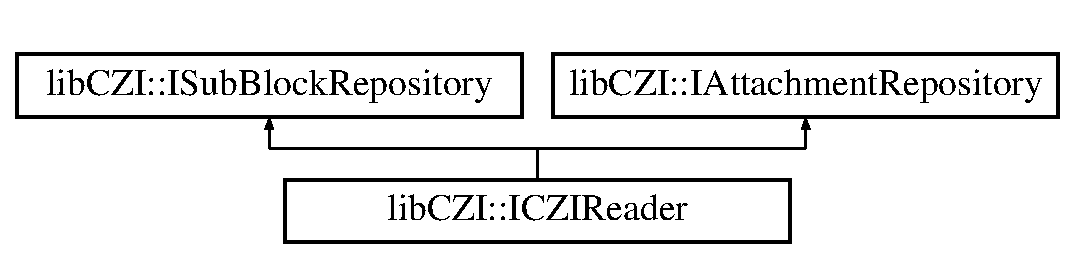
\includegraphics[height=2.000000cm]{classlib_c_z_i_1_1_i_c_z_i_reader}
\end{center}
\end{figure}
\subsection*{Public Member Functions}
\begin{DoxyCompactItemize}
\item 
virtual void \hyperlink{classlib_c_z_i_1_1_i_c_z_i_reader_ae3b1a8fabae6b70480f0855fe374ecd9}{Open} (std\+::shared\+\_\+ptr$<$ \hyperlink{classlib_c_z_i_1_1_i_stream}{I\+Stream} $>$ stream)=0
\item 
virtual \hyperlink{structlib_c_z_i_1_1_file_header_info}{File\+Header\+Info} \hyperlink{classlib_c_z_i_1_1_i_c_z_i_reader_aeae9420aefeed528808a566c4cfc11a2}{Get\+File\+Header\+Info} ()=0
\item 
virtual std\+::shared\+\_\+ptr$<$ \hyperlink{classlib_c_z_i_1_1_i_metadata_segment}{I\+Metadata\+Segment} $>$ \hyperlink{classlib_c_z_i_1_1_i_c_z_i_reader_a9dbab9ddaa7ae4bcfce3c64ed5eea82d}{Read\+Metadata\+Segment} ()=0
\item 
virtual std\+::shared\+\_\+ptr$<$ \hyperlink{classlib_c_z_i_1_1_i_accessor}{I\+Accessor} $>$ \hyperlink{classlib_c_z_i_1_1_i_c_z_i_reader_a3fe8c576a58058e9bbebb9c9fd5633b0}{Create\+Accessor} (\hyperlink{namespacelib_c_z_i_aa626474324df92c9cdc7258cdb1e677c}{Accessor\+Type} accessor\+Type)=0
\item 
virtual void \hyperlink{classlib_c_z_i_1_1_i_c_z_i_reader_aef45f08b7e9cec6a40ab7ee50285eaba}{Close} ()=0
\item 
std\+::shared\+\_\+ptr$<$ \hyperlink{classlib_c_z_i_1_1_i_single_channel_tile_accessor}{I\+Single\+Channel\+Tile\+Accessor} $>$ \hyperlink{classlib_c_z_i_1_1_i_c_z_i_reader_a41d07167b2005205fc15d6d64ec280b8}{Create\+Single\+Channel\+Tile\+Accessor} ()
\item 
std\+::shared\+\_\+ptr$<$ \hyperlink{classlib_c_z_i_1_1_i_single_channel_pyramid_layer_tile_accessor}{I\+Single\+Channel\+Pyramid\+Layer\+Tile\+Accessor} $>$ \hyperlink{classlib_c_z_i_1_1_i_c_z_i_reader_af7f45db86ad27a90394bf036bfa4e985}{Create\+Single\+Channel\+Pyramid\+Layer\+Tile\+Accessor} ()
\item 
std\+::shared\+\_\+ptr$<$ \hyperlink{classlib_c_z_i_1_1_i_single_channel_scaling_tile_accessor}{I\+Single\+Channel\+Scaling\+Tile\+Accessor} $>$ \hyperlink{classlib_c_z_i_1_1_i_c_z_i_reader_a481f10b35f8f9e8afa05b0e0a3f94d59}{Create\+Single\+Channel\+Scaling\+Tile\+Accessor} ()
\end{DoxyCompactItemize}


\subsection{Detailed Description}
This interface is used to represent the C\+Z\+I-\/file. 

\subsection{Member Function Documentation}
\mbox{\Hypertarget{classlib_c_z_i_1_1_i_c_z_i_reader_aef45f08b7e9cec6a40ab7ee50285eaba}\label{classlib_c_z_i_1_1_i_c_z_i_reader_aef45f08b7e9cec6a40ab7ee50285eaba}} 
\index{lib\+C\+Z\+I\+::\+I\+C\+Z\+I\+Reader@{lib\+C\+Z\+I\+::\+I\+C\+Z\+I\+Reader}!Close@{Close}}
\index{Close@{Close}!lib\+C\+Z\+I\+::\+I\+C\+Z\+I\+Reader@{lib\+C\+Z\+I\+::\+I\+C\+Z\+I\+Reader}}
\subsubsection{\texorpdfstring{Close()}{Close()}}
{\footnotesize\ttfamily virtual void lib\+C\+Z\+I\+::\+I\+C\+Z\+I\+Reader\+::\+Close (\begin{DoxyParamCaption}{ }\end{DoxyParamCaption})\hspace{0.3cm}{\ttfamily [pure virtual]}}

Closes C\+Z\+I-\/reader. The underlying stream-\/object will be released, and further calls to other methods will fail. The stream is also closed when the object is destroyed, so it is usually not necessary to explicitly call {\ttfamily Close}. Also, take care that the ownership of the class must be defined when calling {\ttfamily Close}. \mbox{\Hypertarget{classlib_c_z_i_1_1_i_c_z_i_reader_a3fe8c576a58058e9bbebb9c9fd5633b0}\label{classlib_c_z_i_1_1_i_c_z_i_reader_a3fe8c576a58058e9bbebb9c9fd5633b0}} 
\index{lib\+C\+Z\+I\+::\+I\+C\+Z\+I\+Reader@{lib\+C\+Z\+I\+::\+I\+C\+Z\+I\+Reader}!Create\+Accessor@{Create\+Accessor}}
\index{Create\+Accessor@{Create\+Accessor}!lib\+C\+Z\+I\+::\+I\+C\+Z\+I\+Reader@{lib\+C\+Z\+I\+::\+I\+C\+Z\+I\+Reader}}
\subsubsection{\texorpdfstring{Create\+Accessor()}{CreateAccessor()}}
{\footnotesize\ttfamily virtual std\+::shared\+\_\+ptr$<$\hyperlink{classlib_c_z_i_1_1_i_accessor}{I\+Accessor}$>$ lib\+C\+Z\+I\+::\+I\+C\+Z\+I\+Reader\+::\+Create\+Accessor (\begin{DoxyParamCaption}\item[{\hyperlink{namespacelib_c_z_i_aa626474324df92c9cdc7258cdb1e677c}{Accessor\+Type}}]{accessor\+Type }\end{DoxyParamCaption})\hspace{0.3cm}{\ttfamily [pure virtual]}}

Creates an accessor for the sub-\/blocks. See also the various typed methods\+: {\ttfamily Create\+Single\+Channel\+Tile\+Accessor}, {\ttfamily Create\+Single\+Channel\+Pyramid\+Layer\+Tile\+Accessor} and {\ttfamily Create\+Single\+Channel\+Scaling\+Tile\+Accessor}. \begin{DoxyRemark}{Remarks}
If the class is not operational (i. e. Open was not called or Open was not successful), then an exception of type std\+::logic\+\_\+error is thrown.
\end{DoxyRemark}

\begin{DoxyParams}{Parameters}
{\em accessor\+Type} & The type of the accessor.\\
\hline
\end{DoxyParams}
\begin{DoxyReturn}{Returns}
The accessor (of the requested type). 
\end{DoxyReturn}
\mbox{\Hypertarget{classlib_c_z_i_1_1_i_c_z_i_reader_af7f45db86ad27a90394bf036bfa4e985}\label{classlib_c_z_i_1_1_i_c_z_i_reader_af7f45db86ad27a90394bf036bfa4e985}} 
\index{lib\+C\+Z\+I\+::\+I\+C\+Z\+I\+Reader@{lib\+C\+Z\+I\+::\+I\+C\+Z\+I\+Reader}!Create\+Single\+Channel\+Pyramid\+Layer\+Tile\+Accessor@{Create\+Single\+Channel\+Pyramid\+Layer\+Tile\+Accessor}}
\index{Create\+Single\+Channel\+Pyramid\+Layer\+Tile\+Accessor@{Create\+Single\+Channel\+Pyramid\+Layer\+Tile\+Accessor}!lib\+C\+Z\+I\+::\+I\+C\+Z\+I\+Reader@{lib\+C\+Z\+I\+::\+I\+C\+Z\+I\+Reader}}
\subsubsection{\texorpdfstring{Create\+Single\+Channel\+Pyramid\+Layer\+Tile\+Accessor()}{CreateSingleChannelPyramidLayerTileAccessor()}}
{\footnotesize\ttfamily std\+::shared\+\_\+ptr$<$\hyperlink{classlib_c_z_i_1_1_i_single_channel_pyramid_layer_tile_accessor}{I\+Single\+Channel\+Pyramid\+Layer\+Tile\+Accessor}$>$ lib\+C\+Z\+I\+::\+I\+C\+Z\+I\+Reader\+::\+Create\+Single\+Channel\+Pyramid\+Layer\+Tile\+Accessor (\begin{DoxyParamCaption}{ }\end{DoxyParamCaption})\hspace{0.3cm}{\ttfamily [inline]}}

Creates a single channel pyramid-\/layer accessor. \begin{DoxyReturn}{Returns}
The new single channel tile accessor. 
\end{DoxyReturn}
\mbox{\Hypertarget{classlib_c_z_i_1_1_i_c_z_i_reader_a481f10b35f8f9e8afa05b0e0a3f94d59}\label{classlib_c_z_i_1_1_i_c_z_i_reader_a481f10b35f8f9e8afa05b0e0a3f94d59}} 
\index{lib\+C\+Z\+I\+::\+I\+C\+Z\+I\+Reader@{lib\+C\+Z\+I\+::\+I\+C\+Z\+I\+Reader}!Create\+Single\+Channel\+Scaling\+Tile\+Accessor@{Create\+Single\+Channel\+Scaling\+Tile\+Accessor}}
\index{Create\+Single\+Channel\+Scaling\+Tile\+Accessor@{Create\+Single\+Channel\+Scaling\+Tile\+Accessor}!lib\+C\+Z\+I\+::\+I\+C\+Z\+I\+Reader@{lib\+C\+Z\+I\+::\+I\+C\+Z\+I\+Reader}}
\subsubsection{\texorpdfstring{Create\+Single\+Channel\+Scaling\+Tile\+Accessor()}{CreateSingleChannelScalingTileAccessor()}}
{\footnotesize\ttfamily std\+::shared\+\_\+ptr$<$\hyperlink{classlib_c_z_i_1_1_i_single_channel_scaling_tile_accessor}{I\+Single\+Channel\+Scaling\+Tile\+Accessor}$>$ lib\+C\+Z\+I\+::\+I\+C\+Z\+I\+Reader\+::\+Create\+Single\+Channel\+Scaling\+Tile\+Accessor (\begin{DoxyParamCaption}{ }\end{DoxyParamCaption})\hspace{0.3cm}{\ttfamily [inline]}}

Creates a single channel scaling tile accessor. \begin{DoxyReturn}{Returns}
The new single channel scaling tile accessor. 
\end{DoxyReturn}
\mbox{\Hypertarget{classlib_c_z_i_1_1_i_c_z_i_reader_a41d07167b2005205fc15d6d64ec280b8}\label{classlib_c_z_i_1_1_i_c_z_i_reader_a41d07167b2005205fc15d6d64ec280b8}} 
\index{lib\+C\+Z\+I\+::\+I\+C\+Z\+I\+Reader@{lib\+C\+Z\+I\+::\+I\+C\+Z\+I\+Reader}!Create\+Single\+Channel\+Tile\+Accessor@{Create\+Single\+Channel\+Tile\+Accessor}}
\index{Create\+Single\+Channel\+Tile\+Accessor@{Create\+Single\+Channel\+Tile\+Accessor}!lib\+C\+Z\+I\+::\+I\+C\+Z\+I\+Reader@{lib\+C\+Z\+I\+::\+I\+C\+Z\+I\+Reader}}
\subsubsection{\texorpdfstring{Create\+Single\+Channel\+Tile\+Accessor()}{CreateSingleChannelTileAccessor()}}
{\footnotesize\ttfamily std\+::shared\+\_\+ptr$<$\hyperlink{classlib_c_z_i_1_1_i_single_channel_tile_accessor}{I\+Single\+Channel\+Tile\+Accessor}$>$ lib\+C\+Z\+I\+::\+I\+C\+Z\+I\+Reader\+::\+Create\+Single\+Channel\+Tile\+Accessor (\begin{DoxyParamCaption}{ }\end{DoxyParamCaption})\hspace{0.3cm}{\ttfamily [inline]}}

Creates a single channel tile accessor. \begin{DoxyReturn}{Returns}
The new single channel tile accessor. 
\end{DoxyReturn}
\mbox{\Hypertarget{classlib_c_z_i_1_1_i_c_z_i_reader_aeae9420aefeed528808a566c4cfc11a2}\label{classlib_c_z_i_1_1_i_c_z_i_reader_aeae9420aefeed528808a566c4cfc11a2}} 
\index{lib\+C\+Z\+I\+::\+I\+C\+Z\+I\+Reader@{lib\+C\+Z\+I\+::\+I\+C\+Z\+I\+Reader}!Get\+File\+Header\+Info@{Get\+File\+Header\+Info}}
\index{Get\+File\+Header\+Info@{Get\+File\+Header\+Info}!lib\+C\+Z\+I\+::\+I\+C\+Z\+I\+Reader@{lib\+C\+Z\+I\+::\+I\+C\+Z\+I\+Reader}}
\subsubsection{\texorpdfstring{Get\+File\+Header\+Info()}{GetFileHeaderInfo()}}
{\footnotesize\ttfamily virtual \hyperlink{structlib_c_z_i_1_1_file_header_info}{File\+Header\+Info} lib\+C\+Z\+I\+::\+I\+C\+Z\+I\+Reader\+::\+Get\+File\+Header\+Info (\begin{DoxyParamCaption}{ }\end{DoxyParamCaption})\hspace{0.3cm}{\ttfamily [pure virtual]}}

Gets the file header information. \begin{DoxyReturn}{Returns}
The file header information. 
\end{DoxyReturn}
\mbox{\Hypertarget{classlib_c_z_i_1_1_i_c_z_i_reader_ae3b1a8fabae6b70480f0855fe374ecd9}\label{classlib_c_z_i_1_1_i_c_z_i_reader_ae3b1a8fabae6b70480f0855fe374ecd9}} 
\index{lib\+C\+Z\+I\+::\+I\+C\+Z\+I\+Reader@{lib\+C\+Z\+I\+::\+I\+C\+Z\+I\+Reader}!Open@{Open}}
\index{Open@{Open}!lib\+C\+Z\+I\+::\+I\+C\+Z\+I\+Reader@{lib\+C\+Z\+I\+::\+I\+C\+Z\+I\+Reader}}
\subsubsection{\texorpdfstring{Open()}{Open()}}
{\footnotesize\ttfamily virtual void lib\+C\+Z\+I\+::\+I\+C\+Z\+I\+Reader\+::\+Open (\begin{DoxyParamCaption}\item[{std\+::shared\+\_\+ptr$<$ \hyperlink{classlib_c_z_i_1_1_i_stream}{I\+Stream} $>$}]{stream }\end{DoxyParamCaption})\hspace{0.3cm}{\ttfamily [pure virtual]}}

Opens the specified stream and reads the global information from the C\+Z\+I-\/document. The stream passed in will have its refcount incremented, a reference is held until Close is called (or the instance is destroyed). \begin{DoxyRemark}{Remarks}
If this method is called twice, then an exception of type std\+::logic\+\_\+error is thrown.
\end{DoxyRemark}

\begin{DoxyParams}{Parameters}
{\em stream} & The stream object. \\
\hline
\end{DoxyParams}
\mbox{\Hypertarget{classlib_c_z_i_1_1_i_c_z_i_reader_a9dbab9ddaa7ae4bcfce3c64ed5eea82d}\label{classlib_c_z_i_1_1_i_c_z_i_reader_a9dbab9ddaa7ae4bcfce3c64ed5eea82d}} 
\index{lib\+C\+Z\+I\+::\+I\+C\+Z\+I\+Reader@{lib\+C\+Z\+I\+::\+I\+C\+Z\+I\+Reader}!Read\+Metadata\+Segment@{Read\+Metadata\+Segment}}
\index{Read\+Metadata\+Segment@{Read\+Metadata\+Segment}!lib\+C\+Z\+I\+::\+I\+C\+Z\+I\+Reader@{lib\+C\+Z\+I\+::\+I\+C\+Z\+I\+Reader}}
\subsubsection{\texorpdfstring{Read\+Metadata\+Segment()}{ReadMetadataSegment()}}
{\footnotesize\ttfamily virtual std\+::shared\+\_\+ptr$<$\hyperlink{classlib_c_z_i_1_1_i_metadata_segment}{I\+Metadata\+Segment}$>$ lib\+C\+Z\+I\+::\+I\+C\+Z\+I\+Reader\+::\+Read\+Metadata\+Segment (\begin{DoxyParamCaption}{ }\end{DoxyParamCaption})\hspace{0.3cm}{\ttfamily [pure virtual]}}

Reads the metadata segment from the stream. \begin{DoxyRemark}{Remarks}
If the class is not operational (i. e. Open was not called or Open was not successful), then an exception of type std\+::logic\+\_\+error is thrown.
\end{DoxyRemark}
\begin{DoxyReturn}{Returns}
The metadata segment. 
\end{DoxyReturn}


The documentation for this class was generated from the following file\+:\begin{DoxyCompactItemize}
\item 
lib\+C\+Z\+I/lib\+C\+Z\+I.\+h\end{DoxyCompactItemize}

\hypertarget{classlib_c_z_i_1_1_i_decoder}{}\section{lib\+C\+ZI\+:\+:I\+Decoder Class Reference}
\label{classlib_c_z_i_1_1_i_decoder}\index{lib\+C\+Z\+I\+::\+I\+Decoder@{lib\+C\+Z\+I\+::\+I\+Decoder}}


The interface used for operating image decoder. That is the simplest possible interface at this point...  




{\ttfamily \#include $<$lib\+C\+Z\+I\+\_\+\+Site.\+h$>$}

\subsection*{Public Member Functions}
\begin{DoxyCompactItemize}
\item 
virtual std\+::shared\+\_\+ptr$<$ \hyperlink{classlib_c_z_i_1_1_i_bitmap_data}{lib\+C\+Z\+I\+::\+I\+Bitmap\+Data} $>$ \hyperlink{classlib_c_z_i_1_1_i_decoder_a14733581cd1ba72bd39a156b98b52835}{Decode} (const void $\ast$ptr\+Data, size\+\_\+t size)=0
\end{DoxyCompactItemize}


\subsection{Detailed Description}
The interface used for operating image decoder. That is the simplest possible interface at this point... 

\subsection{Member Function Documentation}
\mbox{\Hypertarget{classlib_c_z_i_1_1_i_decoder_a14733581cd1ba72bd39a156b98b52835}\label{classlib_c_z_i_1_1_i_decoder_a14733581cd1ba72bd39a156b98b52835}} 
\index{lib\+C\+Z\+I\+::\+I\+Decoder@{lib\+C\+Z\+I\+::\+I\+Decoder}!Decode@{Decode}}
\index{Decode@{Decode}!lib\+C\+Z\+I\+::\+I\+Decoder@{lib\+C\+Z\+I\+::\+I\+Decoder}}
\subsubsection{\texorpdfstring{Decode()}{Decode()}}
{\footnotesize\ttfamily virtual std\+::shared\+\_\+ptr$<$\hyperlink{classlib_c_z_i_1_1_i_bitmap_data}{lib\+C\+Z\+I\+::\+I\+Bitmap\+Data}$>$ lib\+C\+Z\+I\+::\+I\+Decoder\+::\+Decode (\begin{DoxyParamCaption}\item[{const void $\ast$}]{ptr\+Data,  }\item[{size\+\_\+t}]{size }\end{DoxyParamCaption})\hspace{0.3cm}{\ttfamily [pure virtual]}}

Passing in a block of raw data, decode the image and return a bitmap object. \begin{DoxyRemark}{Remarks}
This method is intended to be called concurrently, implementors should make no assumption about concurrency.

In case of an error (of whatever kind) the method is expected to throw an exception.
\end{DoxyRemark}

\begin{DoxyParams}{Parameters}
{\em ptr\+Data} & Pointer to a a block of memory (which contains the encoded image). \\
\hline
{\em size} & The size of the memory block pointed by {\ttfamily ptr\+Data}.\\
\hline
\end{DoxyParams}
\begin{DoxyReturn}{Returns}
A bitmap object witht the decoded data. 
\end{DoxyReturn}


The documentation for this class was generated from the following file\+:\begin{DoxyCompactItemize}
\item 
lib\+C\+Z\+I/lib\+C\+Z\+I\+\_\+\+Site.\+h\end{DoxyCompactItemize}

\hypertarget{classlib_c_z_i_1_1_i_dim_bounds}{}\section{lib\+C\+ZI\+:\+:I\+Dim\+Bounds Class Reference}
\label{classlib_c_z_i_1_1_i_dim_bounds}\index{lib\+C\+Z\+I\+::\+I\+Dim\+Bounds@{lib\+C\+Z\+I\+::\+I\+Dim\+Bounds}}


Interface used to represent an interval (for several dimensions).  




{\ttfamily \#include $<$lib\+C\+Z\+I\+\_\+\+Dim\+Coordinate.\+h$>$}

Inheritance diagram for lib\+C\+ZI\+:\+:I\+Dim\+Bounds\+:\begin{figure}[H]
\begin{center}
\leavevmode
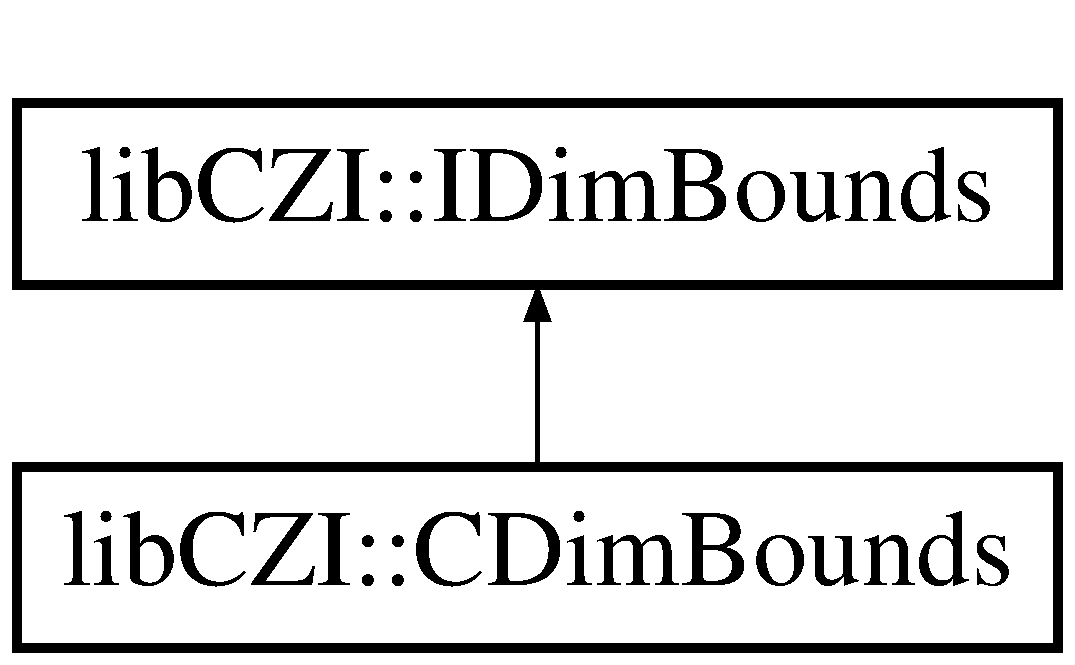
\includegraphics[height=2.000000cm]{classlib_c_z_i_1_1_i_dim_bounds}
\end{center}
\end{figure}
\subsection*{Public Member Functions}
\begin{DoxyCompactItemize}
\item 
virtual bool \hyperlink{classlib_c_z_i_1_1_i_dim_bounds_a7f42cf193370731a6b21ae5d2d6fa78e}{Try\+Get\+Interval} (\hyperlink{namespacelib_c_z_i_a55049658acf59d0eddfaebcad16df424}{Dimension\+Index} dim, int $\ast$start\+Index, int $\ast$size) const =0
\item 
bool \hyperlink{classlib_c_z_i_1_1_i_dim_bounds_ae34c55b6b510804b86383eea5b7c0da9}{Is\+Valid} (\hyperlink{namespacelib_c_z_i_a55049658acf59d0eddfaebcad16df424}{Dimension\+Index} dim) const
\end{DoxyCompactItemize}


\subsection{Detailed Description}
Interface used to represent an interval (for several dimensions). 

\subsection{Member Function Documentation}
\mbox{\Hypertarget{classlib_c_z_i_1_1_i_dim_bounds_ae34c55b6b510804b86383eea5b7c0da9}\label{classlib_c_z_i_1_1_i_dim_bounds_ae34c55b6b510804b86383eea5b7c0da9}} 
\index{lib\+C\+Z\+I\+::\+I\+Dim\+Bounds@{lib\+C\+Z\+I\+::\+I\+Dim\+Bounds}!Is\+Valid@{Is\+Valid}}
\index{Is\+Valid@{Is\+Valid}!lib\+C\+Z\+I\+::\+I\+Dim\+Bounds@{lib\+C\+Z\+I\+::\+I\+Dim\+Bounds}}
\subsubsection{\texorpdfstring{Is\+Valid()}{IsValid()}}
{\footnotesize\ttfamily bool lib\+C\+Z\+I\+::\+I\+Dim\+Bounds\+::\+Is\+Valid (\begin{DoxyParamCaption}\item[{\hyperlink{namespacelib_c_z_i_a55049658acf59d0eddfaebcad16df424}{Dimension\+Index}}]{dim }\end{DoxyParamCaption}) const\hspace{0.3cm}{\ttfamily [inline]}}

Query if the specified dimension is valid. 
\begin{DoxyParams}{Parameters}
{\em dim} & The dimension. \\
\hline
\end{DoxyParams}
\begin{DoxyReturn}{Returns}
True if valid, false otherwise. 
\end{DoxyReturn}
\mbox{\Hypertarget{classlib_c_z_i_1_1_i_dim_bounds_a7f42cf193370731a6b21ae5d2d6fa78e}\label{classlib_c_z_i_1_1_i_dim_bounds_a7f42cf193370731a6b21ae5d2d6fa78e}} 
\index{lib\+C\+Z\+I\+::\+I\+Dim\+Bounds@{lib\+C\+Z\+I\+::\+I\+Dim\+Bounds}!Try\+Get\+Interval@{Try\+Get\+Interval}}
\index{Try\+Get\+Interval@{Try\+Get\+Interval}!lib\+C\+Z\+I\+::\+I\+Dim\+Bounds@{lib\+C\+Z\+I\+::\+I\+Dim\+Bounds}}
\subsubsection{\texorpdfstring{Try\+Get\+Interval()}{TryGetInterval()}}
{\footnotesize\ttfamily virtual bool lib\+C\+Z\+I\+::\+I\+Dim\+Bounds\+::\+Try\+Get\+Interval (\begin{DoxyParamCaption}\item[{\hyperlink{namespacelib_c_z_i_a55049658acf59d0eddfaebcad16df424}{Dimension\+Index}}]{dim,  }\item[{int $\ast$}]{start\+Index,  }\item[{int $\ast$}]{size }\end{DoxyParamCaption}) const\hspace{0.3cm}{\ttfamily [pure virtual]}}

Attempts to get the interval for the specified dimension. 
\begin{DoxyParams}[1]{Parameters}
 & {\em dim} & The dimension. \\
\hline
\mbox{\tt in,out}  & {\em start\+Index} & If non-\/null, it will receive the start index. \\
\hline
\mbox{\tt in,out}  & {\em size} & If non-\/null, it will receive the size. \\
\hline
\end{DoxyParams}
\begin{DoxyReturn}{Returns}
True if the dimension is valid and the data was succeessfully retrieved, false if it fails. 
\end{DoxyReturn}


Implemented in \hyperlink{classlib_c_z_i_1_1_c_dim_bounds_abf42285e28ddc4843556f88b2292c494}{lib\+C\+Z\+I\+::\+C\+Dim\+Bounds}.



The documentation for this class was generated from the following file\+:\begin{DoxyCompactItemize}
\item 
lib\+C\+Z\+I/lib\+C\+Z\+I\+\_\+\+Dim\+Coordinate.\+h\end{DoxyCompactItemize}

\hypertarget{classlib_c_z_i_1_1_i_dim_coordinate}{}\section{lib\+C\+ZI\+:\+:I\+Dim\+Coordinate Class Reference}
\label{classlib_c_z_i_1_1_i_dim_coordinate}\index{lib\+C\+Z\+I\+::\+I\+Dim\+Coordinate@{lib\+C\+Z\+I\+::\+I\+Dim\+Coordinate}}


Interface used to represent a coordinate (in the space of the dimensions identified by {\ttfamily Dimension\+Index}).  




{\ttfamily \#include $<$lib\+C\+Z\+I\+\_\+\+Dim\+Coordinate.\+h$>$}

Inheritance diagram for lib\+C\+ZI\+:\+:I\+Dim\+Coordinate\+:\begin{figure}[H]
\begin{center}
\leavevmode
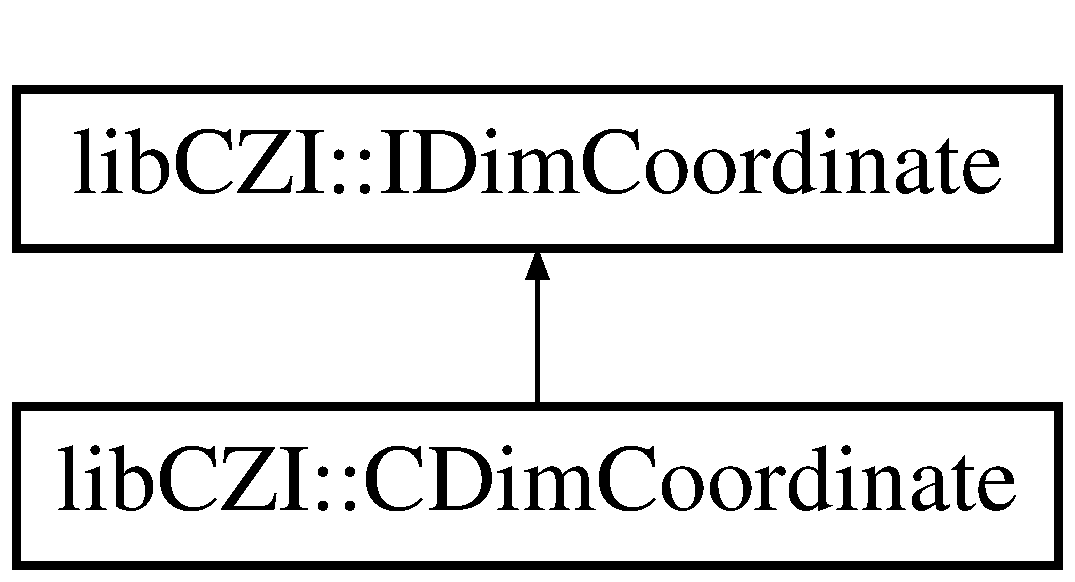
\includegraphics[height=2.000000cm]{classlib_c_z_i_1_1_i_dim_coordinate}
\end{center}
\end{figure}
\subsection*{Public Member Functions}
\begin{DoxyCompactItemize}
\item 
virtual bool \hyperlink{classlib_c_z_i_1_1_i_dim_coordinate_a3b1c18f0102bd5635b3cd9cc3fba69d2}{Try\+Get\+Position} (\hyperlink{namespacelib_c_z_i_a55049658acf59d0eddfaebcad16df424}{Dimension\+Index} dim, int $\ast$coordinate) const =0
\item 
bool \hyperlink{classlib_c_z_i_1_1_i_dim_coordinate_a92dbe2ec439f6c5c47102c51955039e0}{Is\+Valid} (\hyperlink{namespacelib_c_z_i_a55049658acf59d0eddfaebcad16df424}{Dimension\+Index} dim) const
\item 
int \hyperlink{classlib_c_z_i_1_1_i_dim_coordinate_af70c2c0edc0ce4cc15de7a5a0b6442bd}{Get\+Number\+Of\+Valid\+Dimensions} () const
\end{DoxyCompactItemize}


\subsection{Detailed Description}
Interface used to represent a coordinate (in the space of the dimensions identified by {\ttfamily Dimension\+Index}). 

\subsection{Member Function Documentation}
\mbox{\Hypertarget{classlib_c_z_i_1_1_i_dim_coordinate_af70c2c0edc0ce4cc15de7a5a0b6442bd}\label{classlib_c_z_i_1_1_i_dim_coordinate_af70c2c0edc0ce4cc15de7a5a0b6442bd}} 
\index{lib\+C\+Z\+I\+::\+I\+Dim\+Coordinate@{lib\+C\+Z\+I\+::\+I\+Dim\+Coordinate}!Get\+Number\+Of\+Valid\+Dimensions@{Get\+Number\+Of\+Valid\+Dimensions}}
\index{Get\+Number\+Of\+Valid\+Dimensions@{Get\+Number\+Of\+Valid\+Dimensions}!lib\+C\+Z\+I\+::\+I\+Dim\+Coordinate@{lib\+C\+Z\+I\+::\+I\+Dim\+Coordinate}}
\subsubsection{\texorpdfstring{Get\+Number\+Of\+Valid\+Dimensions()}{GetNumberOfValidDimensions()}}
{\footnotesize\ttfamily int lib\+C\+Z\+I\+::\+I\+Dim\+Coordinate\+::\+Get\+Number\+Of\+Valid\+Dimensions (\begin{DoxyParamCaption}{ }\end{DoxyParamCaption}) const\hspace{0.3cm}{\ttfamily [inline]}}

Gets the number of valid dimensions.

\begin{DoxyReturn}{Returns}
The number of valid dimensions. 
\end{DoxyReturn}
\mbox{\Hypertarget{classlib_c_z_i_1_1_i_dim_coordinate_a92dbe2ec439f6c5c47102c51955039e0}\label{classlib_c_z_i_1_1_i_dim_coordinate_a92dbe2ec439f6c5c47102c51955039e0}} 
\index{lib\+C\+Z\+I\+::\+I\+Dim\+Coordinate@{lib\+C\+Z\+I\+::\+I\+Dim\+Coordinate}!Is\+Valid@{Is\+Valid}}
\index{Is\+Valid@{Is\+Valid}!lib\+C\+Z\+I\+::\+I\+Dim\+Coordinate@{lib\+C\+Z\+I\+::\+I\+Dim\+Coordinate}}
\subsubsection{\texorpdfstring{Is\+Valid()}{IsValid()}}
{\footnotesize\ttfamily bool lib\+C\+Z\+I\+::\+I\+Dim\+Coordinate\+::\+Is\+Valid (\begin{DoxyParamCaption}\item[{\hyperlink{namespacelib_c_z_i_a55049658acf59d0eddfaebcad16df424}{Dimension\+Index}}]{dim }\end{DoxyParamCaption}) const\hspace{0.3cm}{\ttfamily [inline]}}

Query if the specified dimension is given (\textquotesingle{}is valid\textquotesingle{}) in this coordinate.


\begin{DoxyParams}{Parameters}
{\em dim} & The dimension.\\
\hline
\end{DoxyParams}
\begin{DoxyReturn}{Returns}
True if the dimension is valid for this coordinate, false if not. 
\end{DoxyReturn}
\mbox{\Hypertarget{classlib_c_z_i_1_1_i_dim_coordinate_a3b1c18f0102bd5635b3cd9cc3fba69d2}\label{classlib_c_z_i_1_1_i_dim_coordinate_a3b1c18f0102bd5635b3cd9cc3fba69d2}} 
\index{lib\+C\+Z\+I\+::\+I\+Dim\+Coordinate@{lib\+C\+Z\+I\+::\+I\+Dim\+Coordinate}!Try\+Get\+Position@{Try\+Get\+Position}}
\index{Try\+Get\+Position@{Try\+Get\+Position}!lib\+C\+Z\+I\+::\+I\+Dim\+Coordinate@{lib\+C\+Z\+I\+::\+I\+Dim\+Coordinate}}
\subsubsection{\texorpdfstring{Try\+Get\+Position()}{TryGetPosition()}}
{\footnotesize\ttfamily virtual bool lib\+C\+Z\+I\+::\+I\+Dim\+Coordinate\+::\+Try\+Get\+Position (\begin{DoxyParamCaption}\item[{\hyperlink{namespacelib_c_z_i_a55049658acf59d0eddfaebcad16df424}{Dimension\+Index}}]{dim,  }\item[{int $\ast$}]{coordinate }\end{DoxyParamCaption}) const\hspace{0.3cm}{\ttfamily [pure virtual]}}

Attempts to get position index in the specified dimension.


\begin{DoxyParams}[1]{Parameters}
 & {\em dim} & The dimension. \\
\hline
\mbox{\tt out}  & {\em coordinate} & If non-\/null and the dimension is valid (in this coordinate), it will receive the value of the coordinate for the specified dimension.\\
\hline
\end{DoxyParams}
\begin{DoxyReturn}{Returns}
True if it succeeds (i. e. the specified dimension is given in this coordinate), false otherwise. 
\end{DoxyReturn}


Implemented in \hyperlink{classlib_c_z_i_1_1_c_dim_coordinate_af7bc7e775a5971d46550e45ebf2b2ba7}{lib\+C\+Z\+I\+::\+C\+Dim\+Coordinate}.



The documentation for this class was generated from the following file\+:\begin{DoxyCompactItemize}
\item 
lib\+C\+Z\+I/lib\+C\+Z\+I\+\_\+\+Dim\+Coordinate.\+h\end{DoxyCompactItemize}

\hypertarget{classlib_c_z_i_1_1_i_dimension_info}{}\section{lib\+C\+ZI\+:\+:I\+Dimension\+Info Class Reference}
\label{classlib_c_z_i_1_1_i_dimension_info}\index{lib\+C\+Z\+I\+::\+I\+Dimension\+Info@{lib\+C\+Z\+I\+::\+I\+Dimension\+Info}}


Base class for information about the dimension.  




{\ttfamily \#include $<$lib\+C\+Z\+I\+\_\+\+Metadata.\+h$>$}

\subsection*{Public Member Functions}
\begin{DoxyCompactItemize}
\item 
virtual \hyperlink{namespacelib_c_z_i_a55049658acf59d0eddfaebcad16df424}{Dimension\+Index} \hyperlink{classlib_c_z_i_1_1_i_dimension_info_a3aef5c6762b0142fc2665d342e939a9d}{Get\+Dimension} () const =0
\item 
virtual void \hyperlink{classlib_c_z_i_1_1_i_dimension_info_a2e04b30f6e8877c3ae080b01e5ff994e}{Get\+Interval} (int $\ast$start, int $\ast$end) const =0
\end{DoxyCompactItemize}


\subsection{Detailed Description}
Base class for information about the dimension. 

\subsection{Member Function Documentation}
\mbox{\Hypertarget{classlib_c_z_i_1_1_i_dimension_info_a3aef5c6762b0142fc2665d342e939a9d}\label{classlib_c_z_i_1_1_i_dimension_info_a3aef5c6762b0142fc2665d342e939a9d}} 
\index{lib\+C\+Z\+I\+::\+I\+Dimension\+Info@{lib\+C\+Z\+I\+::\+I\+Dimension\+Info}!Get\+Dimension@{Get\+Dimension}}
\index{Get\+Dimension@{Get\+Dimension}!lib\+C\+Z\+I\+::\+I\+Dimension\+Info@{lib\+C\+Z\+I\+::\+I\+Dimension\+Info}}
\subsubsection{\texorpdfstring{Get\+Dimension()}{GetDimension()}}
{\footnotesize\ttfamily virtual \hyperlink{namespacelib_c_z_i_a55049658acf59d0eddfaebcad16df424}{Dimension\+Index} lib\+C\+Z\+I\+::\+I\+Dimension\+Info\+::\+Get\+Dimension (\begin{DoxyParamCaption}{ }\end{DoxyParamCaption}) const\hspace{0.3cm}{\ttfamily [pure virtual]}}

Gets the dimension index. \begin{DoxyReturn}{Returns}
The dimension index. 
\end{DoxyReturn}
\mbox{\Hypertarget{classlib_c_z_i_1_1_i_dimension_info_a2e04b30f6e8877c3ae080b01e5ff994e}\label{classlib_c_z_i_1_1_i_dimension_info_a2e04b30f6e8877c3ae080b01e5ff994e}} 
\index{lib\+C\+Z\+I\+::\+I\+Dimension\+Info@{lib\+C\+Z\+I\+::\+I\+Dimension\+Info}!Get\+Interval@{Get\+Interval}}
\index{Get\+Interval@{Get\+Interval}!lib\+C\+Z\+I\+::\+I\+Dimension\+Info@{lib\+C\+Z\+I\+::\+I\+Dimension\+Info}}
\subsubsection{\texorpdfstring{Get\+Interval()}{GetInterval()}}
{\footnotesize\ttfamily virtual void lib\+C\+Z\+I\+::\+I\+Dimension\+Info\+::\+Get\+Interval (\begin{DoxyParamCaption}\item[{int $\ast$}]{start,  }\item[{int $\ast$}]{end }\end{DoxyParamCaption}) const\hspace{0.3cm}{\ttfamily [pure virtual]}}

Gets the interval. 
\begin{DoxyParams}[1]{Parameters}
\mbox{\tt out}  & {\em start} & If non-\/null, it will receive the start index. \\
\hline
\mbox{\tt out}  & {\em end} & If non-\/null, it will receive the end index. \\
\hline
\end{DoxyParams}


The documentation for this class was generated from the following file\+:\begin{DoxyCompactItemize}
\item 
lib\+C\+Z\+I/lib\+C\+Z\+I\+\_\+\+Metadata.\+h\end{DoxyCompactItemize}

\hypertarget{classlib_c_z_i_1_1_i_dimension_t_info}{}\section{lib\+C\+ZI\+:\+:I\+Dimension\+T\+Info Class Reference}
\label{classlib_c_z_i_1_1_i_dimension_t_info}\index{lib\+C\+Z\+I\+::\+I\+Dimension\+T\+Info@{lib\+C\+Z\+I\+::\+I\+Dimension\+T\+Info}}


This structure defines the information for the \char`\"{}\+T-\/dimension\char`\"{}. It resembles the Z\+E\+N-\/metadata-\/structure \char`\"{}\+Dimensions/\+T\char`\"{}.  




{\ttfamily \#include $<$lib\+C\+Z\+I\+\_\+\+Metadata.\+h$>$}

\subsection*{Public Member Functions}
\begin{DoxyCompactItemize}
\item 
virtual bool \hyperlink{classlib_c_z_i_1_1_i_dimension_t_info_ab815fa3e2df4f4d8a243a45e843f9a17}{Try\+Get\+Start\+Time} (\hyperlink{structlib_c_z_i_1_1_xml_date_time}{Xml\+Date\+Time} $\ast$date\+Time)=0
\item 
virtual bool \hyperlink{classlib_c_z_i_1_1_i_dimension_t_info_a524fe50881aaf29353744500f1166158}{Try\+Get\+Interval\+Definition} (double $\ast$offset, double $\ast$increment)=0
\item 
virtual bool \hyperlink{classlib_c_z_i_1_1_i_dimension_t_info_a2c852321a0f26213096c571ccc5f7b65}{Try\+Get\+Offsets\+List} (std\+::vector$<$ double $>$ $\ast$offsets)=0
\end{DoxyCompactItemize}


\subsection{Detailed Description}
This structure defines the information for the \char`\"{}\+T-\/dimension\char`\"{}. It resembles the Z\+E\+N-\/metadata-\/structure \char`\"{}\+Dimensions/\+T\char`\"{}. 

\subsection{Member Function Documentation}
\mbox{\Hypertarget{classlib_c_z_i_1_1_i_dimension_t_info_a524fe50881aaf29353744500f1166158}\label{classlib_c_z_i_1_1_i_dimension_t_info_a524fe50881aaf29353744500f1166158}} 
\index{lib\+C\+Z\+I\+::\+I\+Dimension\+T\+Info@{lib\+C\+Z\+I\+::\+I\+Dimension\+T\+Info}!Try\+Get\+Interval\+Definition@{Try\+Get\+Interval\+Definition}}
\index{Try\+Get\+Interval\+Definition@{Try\+Get\+Interval\+Definition}!lib\+C\+Z\+I\+::\+I\+Dimension\+T\+Info@{lib\+C\+Z\+I\+::\+I\+Dimension\+T\+Info}}
\subsubsection{\texorpdfstring{Try\+Get\+Interval\+Definition()}{TryGetIntervalDefinition()}}
{\footnotesize\ttfamily virtual bool lib\+C\+Z\+I\+::\+I\+Dimension\+T\+Info\+::\+Try\+Get\+Interval\+Definition (\begin{DoxyParamCaption}\item[{double $\ast$}]{offset,  }\item[{double $\ast$}]{increment }\end{DoxyParamCaption})\hspace{0.3cm}{\ttfamily [pure virtual]}}

Attempts to get interval definition which allows to associate a time span with a t-\/index. 
\begin{DoxyParams}[1]{Parameters}
\mbox{\tt in,out}  & {\em offset} & If non-\/null, the offset will be put here (unit\+: second). \\
\hline
\mbox{\tt in,out}  & {\em increment} & If non-\/null, the increment will be put here (unit\+: second). \\
\hline
\end{DoxyParams}
\begin{DoxyReturn}{Returns}
True if it succeeds, false if it fails. 
\end{DoxyReturn}
\mbox{\Hypertarget{classlib_c_z_i_1_1_i_dimension_t_info_a2c852321a0f26213096c571ccc5f7b65}\label{classlib_c_z_i_1_1_i_dimension_t_info_a2c852321a0f26213096c571ccc5f7b65}} 
\index{lib\+C\+Z\+I\+::\+I\+Dimension\+T\+Info@{lib\+C\+Z\+I\+::\+I\+Dimension\+T\+Info}!Try\+Get\+Offsets\+List@{Try\+Get\+Offsets\+List}}
\index{Try\+Get\+Offsets\+List@{Try\+Get\+Offsets\+List}!lib\+C\+Z\+I\+::\+I\+Dimension\+T\+Info@{lib\+C\+Z\+I\+::\+I\+Dimension\+T\+Info}}
\subsubsection{\texorpdfstring{Try\+Get\+Offsets\+List()}{TryGetOffsetsList()}}
{\footnotesize\ttfamily virtual bool lib\+C\+Z\+I\+::\+I\+Dimension\+T\+Info\+::\+Try\+Get\+Offsets\+List (\begin{DoxyParamCaption}\item[{std\+::vector$<$ double $>$ $\ast$}]{offsets }\end{DoxyParamCaption})\hspace{0.3cm}{\ttfamily [pure virtual]}}

Attempts to get the offset list. 
\begin{DoxyParams}[1]{Parameters}
\mbox{\tt in,out}  & {\em offsets} & If non-\/null, the offsets will be put here (unit\+: second). \\
\hline
\end{DoxyParams}
\begin{DoxyReturn}{Returns}
True if it succeeds, false if it fails. 
\end{DoxyReturn}
\mbox{\Hypertarget{classlib_c_z_i_1_1_i_dimension_t_info_ab815fa3e2df4f4d8a243a45e843f9a17}\label{classlib_c_z_i_1_1_i_dimension_t_info_ab815fa3e2df4f4d8a243a45e843f9a17}} 
\index{lib\+C\+Z\+I\+::\+I\+Dimension\+T\+Info@{lib\+C\+Z\+I\+::\+I\+Dimension\+T\+Info}!Try\+Get\+Start\+Time@{Try\+Get\+Start\+Time}}
\index{Try\+Get\+Start\+Time@{Try\+Get\+Start\+Time}!lib\+C\+Z\+I\+::\+I\+Dimension\+T\+Info@{lib\+C\+Z\+I\+::\+I\+Dimension\+T\+Info}}
\subsubsection{\texorpdfstring{Try\+Get\+Start\+Time()}{TryGetStartTime()}}
{\footnotesize\ttfamily virtual bool lib\+C\+Z\+I\+::\+I\+Dimension\+T\+Info\+::\+Try\+Get\+Start\+Time (\begin{DoxyParamCaption}\item[{\hyperlink{structlib_c_z_i_1_1_xml_date_time}{Xml\+Date\+Time} $\ast$}]{date\+Time }\end{DoxyParamCaption})\hspace{0.3cm}{\ttfamily [pure virtual]}}

Attempts to get start time -\/ an absolute point in time which gives the reference point (to which to relative time spans refer to). 
\begin{DoxyParams}[1]{Parameters}
\mbox{\tt in,out}  & {\em date\+Time} & If non-\/null, the reference date time. \\
\hline
\end{DoxyParams}
\begin{DoxyReturn}{Returns}
True if it succeeds, false if it fails. 
\end{DoxyReturn}


The documentation for this class was generated from the following file\+:\begin{DoxyCompactItemize}
\item 
lib\+C\+Z\+I/lib\+C\+Z\+I\+\_\+\+Metadata.\+h\end{DoxyCompactItemize}

\hypertarget{classlib_c_z_i_1_1_i_dimension_z_info}{}\section{lib\+C\+ZI\+:\+:I\+Dimension\+Z\+Info Class Reference}
\label{classlib_c_z_i_1_1_i_dimension_z_info}\index{lib\+C\+Z\+I\+::\+I\+Dimension\+Z\+Info@{lib\+C\+Z\+I\+::\+I\+Dimension\+Z\+Info}}


This structure defines the information for the \char`\"{}\+Z-\/dimension\char`\"{}. It resembles the Z\+E\+N-\/metadata-\/structure \char`\"{}\+Dimensions/\+Z\char`\"{}.  




{\ttfamily \#include $<$lib\+C\+Z\+I\+\_\+\+Metadata.\+h$>$}

\subsection*{Public Types}
\begin{DoxyCompactItemize}
\item 
enum \hyperlink{classlib_c_z_i_1_1_i_dimension_z_info_af1fcb2e3024d14cdcb9122aea7dca121}{Xyz\+Handedness} \+: std\+::uint8\+\_\+t \{ \hyperlink{classlib_c_z_i_1_1_i_dimension_z_info_af1fcb2e3024d14cdcb9122aea7dca121acd5d8803eaa45145192f16041a365ee8}{Xyz\+Handedness\+::\+Left\+Handed}, 
\hyperlink{classlib_c_z_i_1_1_i_dimension_z_info_af1fcb2e3024d14cdcb9122aea7dca121a4583673c474e530a2db116199a93ba82}{Xyz\+Handedness\+::\+Right\+Handed}, 
\hyperlink{classlib_c_z_i_1_1_i_dimension_z_info_af1fcb2e3024d14cdcb9122aea7dca121aec0fc0100c4fc1ce4eea230c3dc10360}{Xyz\+Handedness\+::\+Undefined}
 \}
\item 
enum \hyperlink{classlib_c_z_i_1_1_i_dimension_z_info_a346b5be6ff305bf728939de9b97e9291}{Zaxis\+Direction} \+: std\+::uint8\+\_\+t \{ \hyperlink{classlib_c_z_i_1_1_i_dimension_z_info_a346b5be6ff305bf728939de9b97e9291aaed51d0aebc4405a53cb433bba295738}{Zaxis\+Direction\+::\+From\+Specimen\+To\+Objective}, 
\hyperlink{classlib_c_z_i_1_1_i_dimension_z_info_a346b5be6ff305bf728939de9b97e9291a50427bef20739be87d45e6b4d11697e9}{Zaxis\+Direction\+::\+From\+Objective\+To\+Specimen}, 
\hyperlink{classlib_c_z_i_1_1_i_dimension_z_info_a346b5be6ff305bf728939de9b97e9291aec0fc0100c4fc1ce4eea230c3dc10360}{Zaxis\+Direction\+::\+Undefined}
 \}
\item 
enum \hyperlink{classlib_c_z_i_1_1_i_dimension_z_info_acf54f265a5a03d0aae6cdaca87c09a00}{Z\+Drive\+Mode} \+: std\+::uint8\+\_\+t \{ \hyperlink{classlib_c_z_i_1_1_i_dimension_z_info_acf54f265a5a03d0aae6cdaca87c09a00a535863a82f163709557e59e2eb8139a7}{Z\+Drive\+Mode\+::\+Continuous}, 
\hyperlink{classlib_c_z_i_1_1_i_dimension_z_info_acf54f265a5a03d0aae6cdaca87c09a00a48c7c41b72e1d678923ce3571aa65b2d}{Z\+Drive\+Mode\+::\+Step}
 \}
\end{DoxyCompactItemize}
\subsection*{Public Member Functions}
\begin{DoxyCompactItemize}
\item 
virtual bool \hyperlink{classlib_c_z_i_1_1_i_dimension_z_info_af41653d25ecf78549ad4b5b73d424d81}{Try\+Get\+Reference\+Position} (double $\ast$d)=0
\item 
virtual bool \hyperlink{classlib_c_z_i_1_1_i_dimension_z_info_a74cb2b6c953edf73ee9916e3ab71de3c}{Try\+Get\+Interval\+Definition} (double $\ast$offset, double $\ast$increment)=0
\item 
virtual bool \hyperlink{classlib_c_z_i_1_1_i_dimension_z_info_a457deaa1db474089288081fde2e48e14}{Try\+Get\+Position\+List} (std\+::vector$<$ double $>$ $\ast$positions)=0
\item 
virtual bool \hyperlink{classlib_c_z_i_1_1_i_dimension_z_info_a7047431361b033e2eb258f1565150a09}{Try\+Get\+Xyz\+Handedness} (\hyperlink{classlib_c_z_i_1_1_i_dimension_z_info_af1fcb2e3024d14cdcb9122aea7dca121}{Xyz\+Handedness} $\ast$xyz\+Handedness)=0
\item 
virtual bool \hyperlink{classlib_c_z_i_1_1_i_dimension_z_info_a4a67c41fcf93248e239c249b0e353950}{Try\+Get\+Z\+Axis\+Direction} (\hyperlink{classlib_c_z_i_1_1_i_dimension_z_info_a346b5be6ff305bf728939de9b97e9291}{Zaxis\+Direction} $\ast$z\+Axis\+Direction)=0
\item 
virtual bool \hyperlink{classlib_c_z_i_1_1_i_dimension_z_info_a9cf8c1a2c01152d505c5441c6368b4ba}{Try\+Get\+Z\+Drive\+Mode} (\hyperlink{classlib_c_z_i_1_1_i_dimension_z_info_acf54f265a5a03d0aae6cdaca87c09a00}{Z\+Drive\+Mode} $\ast$zdrivemode)=0
\item 
virtual bool \hyperlink{classlib_c_z_i_1_1_i_dimension_z_info_a9129563d677685df52f4afe6897ef339}{Try\+Z\+Drive\+Speed} (double $\ast$zdrivespeed)=0
\end{DoxyCompactItemize}


\subsection{Detailed Description}
This structure defines the information for the \char`\"{}\+Z-\/dimension\char`\"{}. It resembles the Z\+E\+N-\/metadata-\/structure \char`\"{}\+Dimensions/\+Z\char`\"{}. 

\subsection{Member Enumeration Documentation}
\mbox{\Hypertarget{classlib_c_z_i_1_1_i_dimension_z_info_af1fcb2e3024d14cdcb9122aea7dca121}\label{classlib_c_z_i_1_1_i_dimension_z_info_af1fcb2e3024d14cdcb9122aea7dca121}} 
\index{lib\+C\+Z\+I\+::\+I\+Dimension\+Z\+Info@{lib\+C\+Z\+I\+::\+I\+Dimension\+Z\+Info}!Xyz\+Handedness@{Xyz\+Handedness}}
\index{Xyz\+Handedness@{Xyz\+Handedness}!lib\+C\+Z\+I\+::\+I\+Dimension\+Z\+Info@{lib\+C\+Z\+I\+::\+I\+Dimension\+Z\+Info}}
\subsubsection{\texorpdfstring{Xyz\+Handedness}{XyzHandedness}}
{\footnotesize\ttfamily enum \hyperlink{classlib_c_z_i_1_1_i_dimension_z_info_af1fcb2e3024d14cdcb9122aea7dca121}{lib\+C\+Z\+I\+::\+I\+Dimension\+Z\+Info\+::\+Xyz\+Handedness} \+: std\+::uint8\+\_\+t\hspace{0.3cm}{\ttfamily [strong]}}

Specifies the chirality of the coordinate system defined by
\begin{DoxyItemize}
\item X axis in a subblock, from left to right
\item Y axis in a subblock, from top to bottom(-\/$>$ origin in the top-\/left corner)
\item Z axis given by Z-\/index This chirality is used when arranging the z-\/slices spatially according to their Z-\/index. It is recommended to ensure that the chirality(and the order of the z-\/slices) is unchanged when arranging the z-\/slices according to their associated distances(as given by ../\+Dimensions/\+Z/\+Positions). 
\end{DoxyItemize}\begin{DoxyEnumFields}{Enumerator}
\raisebox{\heightof{T}}[0pt][0pt]{\index{Left\+Handed@{Left\+Handed}!lib\+C\+Z\+I\+::\+I\+Dimension\+Z\+Info@{lib\+C\+Z\+I\+::\+I\+Dimension\+Z\+Info}}\index{lib\+C\+Z\+I\+::\+I\+Dimension\+Z\+Info@{lib\+C\+Z\+I\+::\+I\+Dimension\+Z\+Info}!Left\+Handed@{Left\+Handed}}}\mbox{\Hypertarget{classlib_c_z_i_1_1_i_dimension_z_info_af1fcb2e3024d14cdcb9122aea7dca121acd5d8803eaa45145192f16041a365ee8}\label{classlib_c_z_i_1_1_i_dimension_z_info_af1fcb2e3024d14cdcb9122aea7dca121acd5d8803eaa45145192f16041a365ee8}} 
Left\+Handed&The coordinate-\/system is orientated left-\/handed. \\
\hline

\raisebox{\heightof{T}}[0pt][0pt]{\index{Right\+Handed@{Right\+Handed}!lib\+C\+Z\+I\+::\+I\+Dimension\+Z\+Info@{lib\+C\+Z\+I\+::\+I\+Dimension\+Z\+Info}}\index{lib\+C\+Z\+I\+::\+I\+Dimension\+Z\+Info@{lib\+C\+Z\+I\+::\+I\+Dimension\+Z\+Info}!Right\+Handed@{Right\+Handed}}}\mbox{\Hypertarget{classlib_c_z_i_1_1_i_dimension_z_info_af1fcb2e3024d14cdcb9122aea7dca121a4583673c474e530a2db116199a93ba82}\label{classlib_c_z_i_1_1_i_dimension_z_info_af1fcb2e3024d14cdcb9122aea7dca121a4583673c474e530a2db116199a93ba82}} 
Right\+Handed&The coordinate-\/system is orientated right-\/handed. \\
\hline

\raisebox{\heightof{T}}[0pt][0pt]{\index{Undefined@{Undefined}!lib\+C\+Z\+I\+::\+I\+Dimension\+Z\+Info@{lib\+C\+Z\+I\+::\+I\+Dimension\+Z\+Info}}\index{lib\+C\+Z\+I\+::\+I\+Dimension\+Z\+Info@{lib\+C\+Z\+I\+::\+I\+Dimension\+Z\+Info}!Undefined@{Undefined}}}\mbox{\Hypertarget{classlib_c_z_i_1_1_i_dimension_z_info_af1fcb2e3024d14cdcb9122aea7dca121aec0fc0100c4fc1ce4eea230c3dc10360}\label{classlib_c_z_i_1_1_i_dimension_z_info_af1fcb2e3024d14cdcb9122aea7dca121aec0fc0100c4fc1ce4eea230c3dc10360}} 
Undefined&The coordinate-\/system is undefined. \\
\hline

\end{DoxyEnumFields}
\mbox{\Hypertarget{classlib_c_z_i_1_1_i_dimension_z_info_a346b5be6ff305bf728939de9b97e9291}\label{classlib_c_z_i_1_1_i_dimension_z_info_a346b5be6ff305bf728939de9b97e9291}} 
\index{lib\+C\+Z\+I\+::\+I\+Dimension\+Z\+Info@{lib\+C\+Z\+I\+::\+I\+Dimension\+Z\+Info}!Zaxis\+Direction@{Zaxis\+Direction}}
\index{Zaxis\+Direction@{Zaxis\+Direction}!lib\+C\+Z\+I\+::\+I\+Dimension\+Z\+Info@{lib\+C\+Z\+I\+::\+I\+Dimension\+Z\+Info}}
\subsubsection{\texorpdfstring{Zaxis\+Direction}{ZaxisDirection}}
{\footnotesize\ttfamily enum \hyperlink{classlib_c_z_i_1_1_i_dimension_z_info_a346b5be6ff305bf728939de9b97e9291}{lib\+C\+Z\+I\+::\+I\+Dimension\+Z\+Info\+::\+Zaxis\+Direction} \+: std\+::uint8\+\_\+t\hspace{0.3cm}{\ttfamily [strong]}}

We define the z-\/axis to be collinear with the optical axis. On this axis the z-\/coordinates of the focal plane are measured, and their distances are found in the Z-\/labels (defined under ../\+Dimensions/\+Z/\+Positions) and the Focus\+Position-\/field found in subblock-\/metadata. The direction of the axis may either be �from specimen to objective� or �from objective to specimen�. In this coordinate system the specimen is at a fixed position.\+Note that the origin of the coordinate system is {\itshape not} defined here. Possible values are\+: From\+Specimen\+To\+Objective, From\+Objective\+To\+Specimen and undefined. Undefined is the default (and to be assumed if this element is not present). Note that the coordinate system defined here is different to the one defined with \char`\"{}\+X\+Y\+Z\+Handedness\char`\"{}. \begin{DoxyEnumFields}{Enumerator}
\raisebox{\heightof{T}}[0pt][0pt]{\index{From\+Specimen\+To\+Objective@{From\+Specimen\+To\+Objective}!lib\+C\+Z\+I\+::\+I\+Dimension\+Z\+Info@{lib\+C\+Z\+I\+::\+I\+Dimension\+Z\+Info}}\index{lib\+C\+Z\+I\+::\+I\+Dimension\+Z\+Info@{lib\+C\+Z\+I\+::\+I\+Dimension\+Z\+Info}!From\+Specimen\+To\+Objective@{From\+Specimen\+To\+Objective}}}\mbox{\Hypertarget{classlib_c_z_i_1_1_i_dimension_z_info_a346b5be6ff305bf728939de9b97e9291aaed51d0aebc4405a53cb433bba295738}\label{classlib_c_z_i_1_1_i_dimension_z_info_a346b5be6ff305bf728939de9b97e9291aaed51d0aebc4405a53cb433bba295738}} 
From\+Specimen\+To\+Objective&The z-\/axis is pointing from specimen to objective. \\
\hline

\raisebox{\heightof{T}}[0pt][0pt]{\index{From\+Objective\+To\+Specimen@{From\+Objective\+To\+Specimen}!lib\+C\+Z\+I\+::\+I\+Dimension\+Z\+Info@{lib\+C\+Z\+I\+::\+I\+Dimension\+Z\+Info}}\index{lib\+C\+Z\+I\+::\+I\+Dimension\+Z\+Info@{lib\+C\+Z\+I\+::\+I\+Dimension\+Z\+Info}!From\+Objective\+To\+Specimen@{From\+Objective\+To\+Specimen}}}\mbox{\Hypertarget{classlib_c_z_i_1_1_i_dimension_z_info_a346b5be6ff305bf728939de9b97e9291a50427bef20739be87d45e6b4d11697e9}\label{classlib_c_z_i_1_1_i_dimension_z_info_a346b5be6ff305bf728939de9b97e9291a50427bef20739be87d45e6b4d11697e9}} 
From\+Objective\+To\+Specimen&The z-\/axis is pointing from objective to specimen. \\
\hline

\raisebox{\heightof{T}}[0pt][0pt]{\index{Undefined@{Undefined}!lib\+C\+Z\+I\+::\+I\+Dimension\+Z\+Info@{lib\+C\+Z\+I\+::\+I\+Dimension\+Z\+Info}}\index{lib\+C\+Z\+I\+::\+I\+Dimension\+Z\+Info@{lib\+C\+Z\+I\+::\+I\+Dimension\+Z\+Info}!Undefined@{Undefined}}}\mbox{\Hypertarget{classlib_c_z_i_1_1_i_dimension_z_info_a346b5be6ff305bf728939de9b97e9291aec0fc0100c4fc1ce4eea230c3dc10360}\label{classlib_c_z_i_1_1_i_dimension_z_info_a346b5be6ff305bf728939de9b97e9291aec0fc0100c4fc1ce4eea230c3dc10360}} 
Undefined&This parameter is undefined. \\
\hline

\end{DoxyEnumFields}
\mbox{\Hypertarget{classlib_c_z_i_1_1_i_dimension_z_info_acf54f265a5a03d0aae6cdaca87c09a00}\label{classlib_c_z_i_1_1_i_dimension_z_info_acf54f265a5a03d0aae6cdaca87c09a00}} 
\index{lib\+C\+Z\+I\+::\+I\+Dimension\+Z\+Info@{lib\+C\+Z\+I\+::\+I\+Dimension\+Z\+Info}!Z\+Drive\+Mode@{Z\+Drive\+Mode}}
\index{Z\+Drive\+Mode@{Z\+Drive\+Mode}!lib\+C\+Z\+I\+::\+I\+Dimension\+Z\+Info@{lib\+C\+Z\+I\+::\+I\+Dimension\+Z\+Info}}
\subsubsection{\texorpdfstring{Z\+Drive\+Mode}{ZDriveMode}}
{\footnotesize\ttfamily enum \hyperlink{classlib_c_z_i_1_1_i_dimension_z_info_acf54f265a5a03d0aae6cdaca87c09a00}{lib\+C\+Z\+I\+::\+I\+Dimension\+Z\+Info\+::\+Z\+Drive\+Mode} \+: std\+::uint8\+\_\+t\hspace{0.3cm}{\ttfamily [strong]}}

Description of mode of operation of the Z-\/\+Drive. \char`\"{}\+Continuous\char`\"{} means that the z -\/ drive did not stop while acquiring the image. \char`\"{}\+Step\char`\"{} means that the Z -\/ drive did not move during the acquisition of the image. Used for S\+P\+IM. \begin{DoxyEnumFields}{Enumerator}
\raisebox{\heightof{T}}[0pt][0pt]{\index{Continuous@{Continuous}!lib\+C\+Z\+I\+::\+I\+Dimension\+Z\+Info@{lib\+C\+Z\+I\+::\+I\+Dimension\+Z\+Info}}\index{lib\+C\+Z\+I\+::\+I\+Dimension\+Z\+Info@{lib\+C\+Z\+I\+::\+I\+Dimension\+Z\+Info}!Continuous@{Continuous}}}\mbox{\Hypertarget{classlib_c_z_i_1_1_i_dimension_z_info_acf54f265a5a03d0aae6cdaca87c09a00a535863a82f163709557e59e2eb8139a7}\label{classlib_c_z_i_1_1_i_dimension_z_info_acf54f265a5a03d0aae6cdaca87c09a00a535863a82f163709557e59e2eb8139a7}} 
Continuous&The z-\/drive did not stop while acquiring the image. \\
\hline

\raisebox{\heightof{T}}[0pt][0pt]{\index{Step@{Step}!lib\+C\+Z\+I\+::\+I\+Dimension\+Z\+Info@{lib\+C\+Z\+I\+::\+I\+Dimension\+Z\+Info}}\index{lib\+C\+Z\+I\+::\+I\+Dimension\+Z\+Info@{lib\+C\+Z\+I\+::\+I\+Dimension\+Z\+Info}!Step@{Step}}}\mbox{\Hypertarget{classlib_c_z_i_1_1_i_dimension_z_info_acf54f265a5a03d0aae6cdaca87c09a00a48c7c41b72e1d678923ce3571aa65b2d}\label{classlib_c_z_i_1_1_i_dimension_z_info_acf54f265a5a03d0aae6cdaca87c09a00a48c7c41b72e1d678923ce3571aa65b2d}} 
Step&The z-\/drive did not move during the acquisition of the image. \\
\hline

\end{DoxyEnumFields}


\subsection{Member Function Documentation}
\mbox{\Hypertarget{classlib_c_z_i_1_1_i_dimension_z_info_a74cb2b6c953edf73ee9916e3ab71de3c}\label{classlib_c_z_i_1_1_i_dimension_z_info_a74cb2b6c953edf73ee9916e3ab71de3c}} 
\index{lib\+C\+Z\+I\+::\+I\+Dimension\+Z\+Info@{lib\+C\+Z\+I\+::\+I\+Dimension\+Z\+Info}!Try\+Get\+Interval\+Definition@{Try\+Get\+Interval\+Definition}}
\index{Try\+Get\+Interval\+Definition@{Try\+Get\+Interval\+Definition}!lib\+C\+Z\+I\+::\+I\+Dimension\+Z\+Info@{lib\+C\+Z\+I\+::\+I\+Dimension\+Z\+Info}}
\subsubsection{\texorpdfstring{Try\+Get\+Interval\+Definition()}{TryGetIntervalDefinition()}}
{\footnotesize\ttfamily virtual bool lib\+C\+Z\+I\+::\+I\+Dimension\+Z\+Info\+::\+Try\+Get\+Interval\+Definition (\begin{DoxyParamCaption}\item[{double $\ast$}]{offset,  }\item[{double $\ast$}]{increment }\end{DoxyParamCaption})\hspace{0.3cm}{\ttfamily [pure virtual]}}

Attempts to get interval definition for the z-\/positions. 
\begin{DoxyParams}[1]{Parameters}
\mbox{\tt in,out}  & {\em offset} & If non-\/null and the method was successful, the offset is stored here. \\
\hline
\mbox{\tt in,out}  & {\em increment} & If non-\/null and the method was successful, the increment is stored here. \\
\hline
\end{DoxyParams}
\begin{DoxyReturn}{Returns}
True if it succeeds, false if it fails. 
\end{DoxyReturn}
\mbox{\Hypertarget{classlib_c_z_i_1_1_i_dimension_z_info_a457deaa1db474089288081fde2e48e14}\label{classlib_c_z_i_1_1_i_dimension_z_info_a457deaa1db474089288081fde2e48e14}} 
\index{lib\+C\+Z\+I\+::\+I\+Dimension\+Z\+Info@{lib\+C\+Z\+I\+::\+I\+Dimension\+Z\+Info}!Try\+Get\+Position\+List@{Try\+Get\+Position\+List}}
\index{Try\+Get\+Position\+List@{Try\+Get\+Position\+List}!lib\+C\+Z\+I\+::\+I\+Dimension\+Z\+Info@{lib\+C\+Z\+I\+::\+I\+Dimension\+Z\+Info}}
\subsubsection{\texorpdfstring{Try\+Get\+Position\+List()}{TryGetPositionList()}}
{\footnotesize\ttfamily virtual bool lib\+C\+Z\+I\+::\+I\+Dimension\+Z\+Info\+::\+Try\+Get\+Position\+List (\begin{DoxyParamCaption}\item[{std\+::vector$<$ double $>$ $\ast$}]{positions }\end{DoxyParamCaption})\hspace{0.3cm}{\ttfamily [pure virtual]}}

Attempts to get list definition for the z-\/positions. 
\begin{DoxyParams}[1]{Parameters}
\mbox{\tt in,out}  & {\em positions} & If non-\/null and the method was successful, the list of positions is stored here. \\
\hline
\end{DoxyParams}
\begin{DoxyReturn}{Returns}
True if it succeeds, false if it fails. 
\end{DoxyReturn}
\mbox{\Hypertarget{classlib_c_z_i_1_1_i_dimension_z_info_af41653d25ecf78549ad4b5b73d424d81}\label{classlib_c_z_i_1_1_i_dimension_z_info_af41653d25ecf78549ad4b5b73d424d81}} 
\index{lib\+C\+Z\+I\+::\+I\+Dimension\+Z\+Info@{lib\+C\+Z\+I\+::\+I\+Dimension\+Z\+Info}!Try\+Get\+Reference\+Position@{Try\+Get\+Reference\+Position}}
\index{Try\+Get\+Reference\+Position@{Try\+Get\+Reference\+Position}!lib\+C\+Z\+I\+::\+I\+Dimension\+Z\+Info@{lib\+C\+Z\+I\+::\+I\+Dimension\+Z\+Info}}
\subsubsection{\texorpdfstring{Try\+Get\+Reference\+Position()}{TryGetReferencePosition()}}
{\footnotesize\ttfamily virtual bool lib\+C\+Z\+I\+::\+I\+Dimension\+Z\+Info\+::\+Try\+Get\+Reference\+Position (\begin{DoxyParamCaption}\item[{double $\ast$}]{d }\end{DoxyParamCaption})\hspace{0.3cm}{\ttfamily [pure virtual]}}

Gets the reference position in units of �m. If this is not valid, then the Z-\/positions only have a relative meaning. 
\begin{DoxyParams}[1]{Parameters}
\mbox{\tt in,out}  & {\em d} & If non-\/null, the double will receive the requested value if successful. \\
\hline
\end{DoxyParams}
\begin{DoxyReturn}{Returns}
True if it succeeds, false if it fails. 
\end{DoxyReturn}
\mbox{\Hypertarget{classlib_c_z_i_1_1_i_dimension_z_info_a7047431361b033e2eb258f1565150a09}\label{classlib_c_z_i_1_1_i_dimension_z_info_a7047431361b033e2eb258f1565150a09}} 
\index{lib\+C\+Z\+I\+::\+I\+Dimension\+Z\+Info@{lib\+C\+Z\+I\+::\+I\+Dimension\+Z\+Info}!Try\+Get\+Xyz\+Handedness@{Try\+Get\+Xyz\+Handedness}}
\index{Try\+Get\+Xyz\+Handedness@{Try\+Get\+Xyz\+Handedness}!lib\+C\+Z\+I\+::\+I\+Dimension\+Z\+Info@{lib\+C\+Z\+I\+::\+I\+Dimension\+Z\+Info}}
\subsubsection{\texorpdfstring{Try\+Get\+Xyz\+Handedness()}{TryGetXyzHandedness()}}
{\footnotesize\ttfamily virtual bool lib\+C\+Z\+I\+::\+I\+Dimension\+Z\+Info\+::\+Try\+Get\+Xyz\+Handedness (\begin{DoxyParamCaption}\item[{\hyperlink{classlib_c_z_i_1_1_i_dimension_z_info_af1fcb2e3024d14cdcb9122aea7dca121}{Xyz\+Handedness} $\ast$}]{xyz\+Handedness }\end{DoxyParamCaption})\hspace{0.3cm}{\ttfamily [pure virtual]}}

Attempts to get X\+Y\+Z-\/handedness property. 
\begin{DoxyParams}[1]{Parameters}
\mbox{\tt in,out}  & {\em xyz\+Handedness} & If non-\/null and the method was successful, the X\+Y\+Z-\/handedness is stored here. \\
\hline
\end{DoxyParams}
\begin{DoxyReturn}{Returns}
True if it succeeds, false if it fails. 
\end{DoxyReturn}
\mbox{\Hypertarget{classlib_c_z_i_1_1_i_dimension_z_info_a4a67c41fcf93248e239c249b0e353950}\label{classlib_c_z_i_1_1_i_dimension_z_info_a4a67c41fcf93248e239c249b0e353950}} 
\index{lib\+C\+Z\+I\+::\+I\+Dimension\+Z\+Info@{lib\+C\+Z\+I\+::\+I\+Dimension\+Z\+Info}!Try\+Get\+Z\+Axis\+Direction@{Try\+Get\+Z\+Axis\+Direction}}
\index{Try\+Get\+Z\+Axis\+Direction@{Try\+Get\+Z\+Axis\+Direction}!lib\+C\+Z\+I\+::\+I\+Dimension\+Z\+Info@{lib\+C\+Z\+I\+::\+I\+Dimension\+Z\+Info}}
\subsubsection{\texorpdfstring{Try\+Get\+Z\+Axis\+Direction()}{TryGetZAxisDirection()}}
{\footnotesize\ttfamily virtual bool lib\+C\+Z\+I\+::\+I\+Dimension\+Z\+Info\+::\+Try\+Get\+Z\+Axis\+Direction (\begin{DoxyParamCaption}\item[{\hyperlink{classlib_c_z_i_1_1_i_dimension_z_info_a346b5be6ff305bf728939de9b97e9291}{Zaxis\+Direction} $\ast$}]{z\+Axis\+Direction }\end{DoxyParamCaption})\hspace{0.3cm}{\ttfamily [pure virtual]}}

Attempts to get Z-\/axis direction property. 
\begin{DoxyParams}[1]{Parameters}
\mbox{\tt in,out}  & {\em z\+Axis\+Direction} & If non-\/null and the method was successful, the Z-\/axis direction is stored here. \\
\hline
\end{DoxyParams}
\begin{DoxyReturn}{Returns}
True if it succeeds, false if it fails. 
\end{DoxyReturn}
\mbox{\Hypertarget{classlib_c_z_i_1_1_i_dimension_z_info_a9cf8c1a2c01152d505c5441c6368b4ba}\label{classlib_c_z_i_1_1_i_dimension_z_info_a9cf8c1a2c01152d505c5441c6368b4ba}} 
\index{lib\+C\+Z\+I\+::\+I\+Dimension\+Z\+Info@{lib\+C\+Z\+I\+::\+I\+Dimension\+Z\+Info}!Try\+Get\+Z\+Drive\+Mode@{Try\+Get\+Z\+Drive\+Mode}}
\index{Try\+Get\+Z\+Drive\+Mode@{Try\+Get\+Z\+Drive\+Mode}!lib\+C\+Z\+I\+::\+I\+Dimension\+Z\+Info@{lib\+C\+Z\+I\+::\+I\+Dimension\+Z\+Info}}
\subsubsection{\texorpdfstring{Try\+Get\+Z\+Drive\+Mode()}{TryGetZDriveMode()}}
{\footnotesize\ttfamily virtual bool lib\+C\+Z\+I\+::\+I\+Dimension\+Z\+Info\+::\+Try\+Get\+Z\+Drive\+Mode (\begin{DoxyParamCaption}\item[{\hyperlink{classlib_c_z_i_1_1_i_dimension_z_info_acf54f265a5a03d0aae6cdaca87c09a00}{Z\+Drive\+Mode} $\ast$}]{zdrivemode }\end{DoxyParamCaption})\hspace{0.3cm}{\ttfamily [pure virtual]}}

Attempts to get Z-\/drive mode property. 
\begin{DoxyParams}[1]{Parameters}
\mbox{\tt in,out}  & {\em zdrivemode} & If non-\/null and the method was successful, the Z-\/drive mode is stored here. \\
\hline
\end{DoxyParams}
\begin{DoxyReturn}{Returns}
True if it succeeds, false if it fails. 
\end{DoxyReturn}
\mbox{\Hypertarget{classlib_c_z_i_1_1_i_dimension_z_info_a9129563d677685df52f4afe6897ef339}\label{classlib_c_z_i_1_1_i_dimension_z_info_a9129563d677685df52f4afe6897ef339}} 
\index{lib\+C\+Z\+I\+::\+I\+Dimension\+Z\+Info@{lib\+C\+Z\+I\+::\+I\+Dimension\+Z\+Info}!Try\+Z\+Drive\+Speed@{Try\+Z\+Drive\+Speed}}
\index{Try\+Z\+Drive\+Speed@{Try\+Z\+Drive\+Speed}!lib\+C\+Z\+I\+::\+I\+Dimension\+Z\+Info@{lib\+C\+Z\+I\+::\+I\+Dimension\+Z\+Info}}
\subsubsection{\texorpdfstring{Try\+Z\+Drive\+Speed()}{TryZDriveSpeed()}}
{\footnotesize\ttfamily virtual bool lib\+C\+Z\+I\+::\+I\+Dimension\+Z\+Info\+::\+Try\+Z\+Drive\+Speed (\begin{DoxyParamCaption}\item[{double $\ast$}]{zdrivespeed }\end{DoxyParamCaption})\hspace{0.3cm}{\ttfamily [pure virtual]}}

Attempts to get the z-\/drive speed (in units of �m/s). 
\begin{DoxyParams}[1]{Parameters}
\mbox{\tt in,out}  & {\em zdrivespeed} & If non-\/null and the method was successful, the z-\/drive speed is stored here. \\
\hline
\end{DoxyParams}
\begin{DoxyReturn}{Returns}
True if it succeeds, false if it fails. 
\end{DoxyReturn}


The documentation for this class was generated from the following file\+:\begin{DoxyCompactItemize}
\item 
lib\+C\+Z\+I/lib\+C\+Z\+I\+\_\+\+Metadata.\+h\end{DoxyCompactItemize}

\hypertarget{classlib_c_z_i_1_1_i_display_settings}{}\section{lib\+C\+ZI\+:\+:I\+Display\+Settings Class Reference}
\label{classlib_c_z_i_1_1_i_display_settings}\index{lib\+C\+Z\+I\+::\+I\+Display\+Settings@{lib\+C\+Z\+I\+::\+I\+Display\+Settings}}


The display settings.  




{\ttfamily \#include $<$lib\+C\+Z\+I\+\_\+\+Metadata.\+h$>$}

\subsection*{Classes}
\begin{DoxyCompactItemize}
\item 
struct \hyperlink{structlib_c_z_i_1_1_i_display_settings_1_1_cubic_spline_coefficients}{Cubic\+Spline\+Coefficients}
\begin{DoxyCompactList}\small\item\em The coefficients of a cubic spline defined by $a\,x^3 + b\,x^2 + c\,x + d =y$. \end{DoxyCompactList}\item 
struct \hyperlink{structlib_c_z_i_1_1_i_display_settings_1_1_spline_control_point}{Spline\+Control\+Point}
\begin{DoxyCompactList}\small\item\em The (normalized) control points of a spline. \end{DoxyCompactList}\item 
struct \hyperlink{structlib_c_z_i_1_1_i_display_settings_1_1_spline_data}{Spline\+Data}
\begin{DoxyCompactList}\small\item\em The defintion of the (piecewise) spline. The spline starts at {\ttfamily x\+Pos} which is the normalized position (between 0 and 1). \end{DoxyCompactList}\end{DoxyCompactItemize}
\subsection*{Public Types}
\begin{DoxyCompactItemize}
\item 
enum \hyperlink{classlib_c_z_i_1_1_i_display_settings_af114dfcc8a603ca1c2fc57bc35c97684}{Gradation\+Curve\+Mode} \+: std\+::uint8\+\_\+t \{ \hyperlink{classlib_c_z_i_1_1_i_display_settings_af114dfcc8a603ca1c2fc57bc35c97684a32a843da6ea40ab3b17a3421ccdf671b}{Gradation\+Curve\+Mode\+::\+Linear}, 
\hyperlink{classlib_c_z_i_1_1_i_display_settings_af114dfcc8a603ca1c2fc57bc35c97684ad9cdb0f6e0d556347c10a8695545a4b5}{Gradation\+Curve\+Mode\+::\+Gamma}, 
\hyperlink{classlib_c_z_i_1_1_i_display_settings_af114dfcc8a603ca1c2fc57bc35c97684a4cff6afc4963881749f7742fbb4d1392}{Gradation\+Curve\+Mode\+::\+Spline}
 \}\begin{DoxyCompactList}\small\item\em Values that represent the gradation curve modes. \end{DoxyCompactList}
\item 
enum \hyperlink{classlib_c_z_i_1_1_i_display_settings_a5a69bda933a814a09f15983606047876}{Tinting\+Mode} \+: std\+::uint8\+\_\+t \{ \hyperlink{classlib_c_z_i_1_1_i_display_settings_a5a69bda933a814a09f15983606047876a6adf97f83acf6453d4a6a4b1070f3754}{Tinting\+Mode\+::\+None} = 0, 
\hyperlink{classlib_c_z_i_1_1_i_display_settings_a5a69bda933a814a09f15983606047876acb5feb1b7314637725a2e73bdc9f7295}{Tinting\+Mode\+::\+Color} = 1, 
\hyperlink{classlib_c_z_i_1_1_i_display_settings_a5a69bda933a814a09f15983606047876a61f8182e36d4c95e5189d83abe8ef4db}{Tinting\+Mode\+::\+Look\+Up\+Table\+Explicit} = 2, 
\hyperlink{classlib_c_z_i_1_1_i_display_settings_a5a69bda933a814a09f15983606047876a39e07c28126f2fe17c07b25db1adfa2d}{Tinting\+Mode\+::\+Look\+Up\+Table\+Well\+Known} = 3
 \}
\end{DoxyCompactItemize}
\subsection*{Public Member Functions}
\begin{DoxyCompactItemize}
\item 
virtual void \hyperlink{classlib_c_z_i_1_1_i_display_settings_af19480abbb7905656e5411bd34d0506d}{Enum\+Channels} (std\+::function$<$ bool(int ch\+Index)$>$ func) const =0
\item 
virtual std\+::shared\+\_\+ptr$<$ \hyperlink{classlib_c_z_i_1_1_i_channel_display_setting}{lib\+C\+Z\+I\+::\+I\+Channel\+Display\+Setting} $>$ \hyperlink{classlib_c_z_i_1_1_i_display_settings_ad67ab35e429286d38dd11245eda3dc4c}{Get\+Channel\+Display\+Settings} (int ch\+Index) const =0
\end{DoxyCompactItemize}
\subsection*{Static Public Member Functions}
\begin{DoxyCompactItemize}
\item 
static void \hyperlink{classlib_c_z_i_1_1_i_display_settings_a0120cb7865379fc27912489dc20bbd01}{Clone} (const \hyperlink{classlib_c_z_i_1_1_i_display_settings}{I\+Display\+Settings} $\ast$disp, \hyperlink{structlib_c_z_i_1_1_display_settings_p_o_d}{Display\+Settings\+P\+OD} \&pod)
\end{DoxyCompactItemize}


\subsection{Detailed Description}
The display settings. 

\subsection{Member Enumeration Documentation}
\mbox{\Hypertarget{classlib_c_z_i_1_1_i_display_settings_af114dfcc8a603ca1c2fc57bc35c97684}\label{classlib_c_z_i_1_1_i_display_settings_af114dfcc8a603ca1c2fc57bc35c97684}} 
\index{lib\+C\+Z\+I\+::\+I\+Display\+Settings@{lib\+C\+Z\+I\+::\+I\+Display\+Settings}!Gradation\+Curve\+Mode@{Gradation\+Curve\+Mode}}
\index{Gradation\+Curve\+Mode@{Gradation\+Curve\+Mode}!lib\+C\+Z\+I\+::\+I\+Display\+Settings@{lib\+C\+Z\+I\+::\+I\+Display\+Settings}}
\subsubsection{\texorpdfstring{Gradation\+Curve\+Mode}{GradationCurveMode}}
{\footnotesize\ttfamily enum \hyperlink{classlib_c_z_i_1_1_i_display_settings_af114dfcc8a603ca1c2fc57bc35c97684}{lib\+C\+Z\+I\+::\+I\+Display\+Settings\+::\+Gradation\+Curve\+Mode} \+: std\+::uint8\+\_\+t\hspace{0.3cm}{\ttfamily [strong]}}



Values that represent the gradation curve modes. 

\begin{DoxyEnumFields}{Enumerator}
\raisebox{\heightof{T}}[0pt][0pt]{\index{Linear@{Linear}!lib\+C\+Z\+I\+::\+I\+Display\+Settings@{lib\+C\+Z\+I\+::\+I\+Display\+Settings}}\index{lib\+C\+Z\+I\+::\+I\+Display\+Settings@{lib\+C\+Z\+I\+::\+I\+Display\+Settings}!Linear@{Linear}}}\mbox{\Hypertarget{classlib_c_z_i_1_1_i_display_settings_af114dfcc8a603ca1c2fc57bc35c97684a32a843da6ea40ab3b17a3421ccdf671b}\label{classlib_c_z_i_1_1_i_display_settings_af114dfcc8a603ca1c2fc57bc35c97684a32a843da6ea40ab3b17a3421ccdf671b}} 
Linear&The gradation curve is a straight line (from white point to black point). \\
\hline

\raisebox{\heightof{T}}[0pt][0pt]{\index{Gamma@{Gamma}!lib\+C\+Z\+I\+::\+I\+Display\+Settings@{lib\+C\+Z\+I\+::\+I\+Display\+Settings}}\index{lib\+C\+Z\+I\+::\+I\+Display\+Settings@{lib\+C\+Z\+I\+::\+I\+Display\+Settings}!Gamma@{Gamma}}}\mbox{\Hypertarget{classlib_c_z_i_1_1_i_display_settings_af114dfcc8a603ca1c2fc57bc35c97684ad9cdb0f6e0d556347c10a8695545a4b5}\label{classlib_c_z_i_1_1_i_display_settings_af114dfcc8a603ca1c2fc57bc35c97684ad9cdb0f6e0d556347c10a8695545a4b5}} 
Gamma&The gradation curve is defined by a gamma. \\
\hline

\raisebox{\heightof{T}}[0pt][0pt]{\index{Spline@{Spline}!lib\+C\+Z\+I\+::\+I\+Display\+Settings@{lib\+C\+Z\+I\+::\+I\+Display\+Settings}}\index{lib\+C\+Z\+I\+::\+I\+Display\+Settings@{lib\+C\+Z\+I\+::\+I\+Display\+Settings}!Spline@{Spline}}}\mbox{\Hypertarget{classlib_c_z_i_1_1_i_display_settings_af114dfcc8a603ca1c2fc57bc35c97684a4cff6afc4963881749f7742fbb4d1392}\label{classlib_c_z_i_1_1_i_display_settings_af114dfcc8a603ca1c2fc57bc35c97684a4cff6afc4963881749f7742fbb4d1392}} 
Spline&The gradation curve is defined by piecewise splines. \\
\hline

\end{DoxyEnumFields}
\mbox{\Hypertarget{classlib_c_z_i_1_1_i_display_settings_a5a69bda933a814a09f15983606047876}\label{classlib_c_z_i_1_1_i_display_settings_a5a69bda933a814a09f15983606047876}} 
\index{lib\+C\+Z\+I\+::\+I\+Display\+Settings@{lib\+C\+Z\+I\+::\+I\+Display\+Settings}!Tinting\+Mode@{Tinting\+Mode}}
\index{Tinting\+Mode@{Tinting\+Mode}!lib\+C\+Z\+I\+::\+I\+Display\+Settings@{lib\+C\+Z\+I\+::\+I\+Display\+Settings}}
\subsubsection{\texorpdfstring{Tinting\+Mode}{TintingMode}}
{\footnotesize\ttfamily enum \hyperlink{classlib_c_z_i_1_1_i_display_settings_a5a69bda933a814a09f15983606047876}{lib\+C\+Z\+I\+::\+I\+Display\+Settings\+::\+Tinting\+Mode} \+: std\+::uint8\+\_\+t\hspace{0.3cm}{\ttfamily [strong]}}

This enum specifies the \char`\"{}tinting-\/mode\char`\"{} -\/ how the channel is false-\/colored. \begin{DoxyRemark}{Remarks}
Plan is to add a property \char`\"{}\+Get\+Tinting\+Mode\char`\"{}, currently we only implement \char`\"{}\+Color\char`\"{} and \char`\"{}\+None\char`\"{}, so this information is conveniently contained in the method \char`\"{}\+Try\+Get\+Tinting\+Color\+Rgb8\char`\"{}. 
\end{DoxyRemark}
\begin{DoxyEnumFields}{Enumerator}
\raisebox{\heightof{T}}[0pt][0pt]{\index{None@{None}!lib\+C\+Z\+I\+::\+I\+Display\+Settings@{lib\+C\+Z\+I\+::\+I\+Display\+Settings}}\index{lib\+C\+Z\+I\+::\+I\+Display\+Settings@{lib\+C\+Z\+I\+::\+I\+Display\+Settings}!None@{None}}}\mbox{\Hypertarget{classlib_c_z_i_1_1_i_display_settings_a5a69bda933a814a09f15983606047876a6adf97f83acf6453d4a6a4b1070f3754}\label{classlib_c_z_i_1_1_i_display_settings_a5a69bda933a814a09f15983606047876a6adf97f83acf6453d4a6a4b1070f3754}} 
None&None -\/ which gives the \char`\"{}original color\char`\"{}, ie. in case of R\+GB the R\+G\+B-\/value is directly used, in case of grayscale we get a gray pixel. \\
\hline

\raisebox{\heightof{T}}[0pt][0pt]{\index{Color@{Color}!lib\+C\+Z\+I\+::\+I\+Display\+Settings@{lib\+C\+Z\+I\+::\+I\+Display\+Settings}}\index{lib\+C\+Z\+I\+::\+I\+Display\+Settings@{lib\+C\+Z\+I\+::\+I\+Display\+Settings}!Color@{Color}}}\mbox{\Hypertarget{classlib_c_z_i_1_1_i_display_settings_a5a69bda933a814a09f15983606047876acb5feb1b7314637725a2e73bdc9f7295}\label{classlib_c_z_i_1_1_i_display_settings_a5a69bda933a814a09f15983606047876acb5feb1b7314637725a2e73bdc9f7295}} 
Color&The pixel value is multiplied with the tinting-\/color. \\
\hline

\raisebox{\heightof{T}}[0pt][0pt]{\index{Look\+Up\+Table\+Explicit@{Look\+Up\+Table\+Explicit}!lib\+C\+Z\+I\+::\+I\+Display\+Settings@{lib\+C\+Z\+I\+::\+I\+Display\+Settings}}\index{lib\+C\+Z\+I\+::\+I\+Display\+Settings@{lib\+C\+Z\+I\+::\+I\+Display\+Settings}!Look\+Up\+Table\+Explicit@{Look\+Up\+Table\+Explicit}}}\mbox{\Hypertarget{classlib_c_z_i_1_1_i_display_settings_a5a69bda933a814a09f15983606047876a61f8182e36d4c95e5189d83abe8ef4db}\label{classlib_c_z_i_1_1_i_display_settings_a5a69bda933a814a09f15983606047876a61f8182e36d4c95e5189d83abe8ef4db}} 
Look\+Up\+Table\+Explicit&(N\+OT Y\+ET I\+M\+P\+L\+E\+M\+E\+N\+T\+ED) There is an explicit look-\/up-\/table specified. \\
\hline

\raisebox{\heightof{T}}[0pt][0pt]{\index{Look\+Up\+Table\+Well\+Known@{Look\+Up\+Table\+Well\+Known}!lib\+C\+Z\+I\+::\+I\+Display\+Settings@{lib\+C\+Z\+I\+::\+I\+Display\+Settings}}\index{lib\+C\+Z\+I\+::\+I\+Display\+Settings@{lib\+C\+Z\+I\+::\+I\+Display\+Settings}!Look\+Up\+Table\+Well\+Known@{Look\+Up\+Table\+Well\+Known}}}\mbox{\Hypertarget{classlib_c_z_i_1_1_i_display_settings_a5a69bda933a814a09f15983606047876a39e07c28126f2fe17c07b25db1adfa2d}\label{classlib_c_z_i_1_1_i_display_settings_a5a69bda933a814a09f15983606047876a39e07c28126f2fe17c07b25db1adfa2d}} 
Look\+Up\+Table\+Well\+Known&(N\+OT Y\+ET I\+M\+P\+L\+E\+M\+E\+N\+T\+ED) We are using a \char`\"{}well-\/known\char`\"{} look-\/up-\/table, and it is identified by its name (which is a string). \\
\hline

\end{DoxyEnumFields}


\subsection{Member Function Documentation}
\mbox{\Hypertarget{classlib_c_z_i_1_1_i_display_settings_a0120cb7865379fc27912489dc20bbd01}\label{classlib_c_z_i_1_1_i_display_settings_a0120cb7865379fc27912489dc20bbd01}} 
\index{lib\+C\+Z\+I\+::\+I\+Display\+Settings@{lib\+C\+Z\+I\+::\+I\+Display\+Settings}!Clone@{Clone}}
\index{Clone@{Clone}!lib\+C\+Z\+I\+::\+I\+Display\+Settings@{lib\+C\+Z\+I\+::\+I\+Display\+Settings}}
\subsubsection{\texorpdfstring{Clone()}{Clone()}}
{\footnotesize\ttfamily static void lib\+C\+Z\+I\+::\+I\+Display\+Settings\+::\+Clone (\begin{DoxyParamCaption}\item[{const \hyperlink{classlib_c_z_i_1_1_i_display_settings}{I\+Display\+Settings} $\ast$}]{disp,  }\item[{\hyperlink{structlib_c_z_i_1_1_display_settings_p_o_d}{Display\+Settings\+P\+OD} \&}]{pod }\end{DoxyParamCaption})\hspace{0.3cm}{\ttfamily [static]}}

Makes a deep copy of the information in this object and store the information in the P\+OD. 
\begin{DoxyParams}[1]{Parameters}
 & {\em disp} & The display-\/settings object. \\
\hline
\mbox{\tt in,out}  & {\em pod} & The P\+O\+D-\/display-\/settings object to store the information in. \\
\hline
\end{DoxyParams}
\mbox{\Hypertarget{classlib_c_z_i_1_1_i_display_settings_af19480abbb7905656e5411bd34d0506d}\label{classlib_c_z_i_1_1_i_display_settings_af19480abbb7905656e5411bd34d0506d}} 
\index{lib\+C\+Z\+I\+::\+I\+Display\+Settings@{lib\+C\+Z\+I\+::\+I\+Display\+Settings}!Enum\+Channels@{Enum\+Channels}}
\index{Enum\+Channels@{Enum\+Channels}!lib\+C\+Z\+I\+::\+I\+Display\+Settings@{lib\+C\+Z\+I\+::\+I\+Display\+Settings}}
\subsubsection{\texorpdfstring{Enum\+Channels()}{EnumChannels()}}
{\footnotesize\ttfamily virtual void lib\+C\+Z\+I\+::\+I\+Display\+Settings\+::\+Enum\+Channels (\begin{DoxyParamCaption}\item[{std\+::function$<$ bool(int ch\+Index)$>$}]{func }\end{DoxyParamCaption}) const\hspace{0.3cm}{\ttfamily [pure virtual]}}

Enum all channels (which are described by the display-\/settings object).


\begin{DoxyParams}{Parameters}
{\em func} & The functor to be called (passing in the channel index). If the functor returns false, the enumeration is stopped. \\
\hline
\end{DoxyParams}
\mbox{\Hypertarget{classlib_c_z_i_1_1_i_display_settings_ad67ab35e429286d38dd11245eda3dc4c}\label{classlib_c_z_i_1_1_i_display_settings_ad67ab35e429286d38dd11245eda3dc4c}} 
\index{lib\+C\+Z\+I\+::\+I\+Display\+Settings@{lib\+C\+Z\+I\+::\+I\+Display\+Settings}!Get\+Channel\+Display\+Settings@{Get\+Channel\+Display\+Settings}}
\index{Get\+Channel\+Display\+Settings@{Get\+Channel\+Display\+Settings}!lib\+C\+Z\+I\+::\+I\+Display\+Settings@{lib\+C\+Z\+I\+::\+I\+Display\+Settings}}
\subsubsection{\texorpdfstring{Get\+Channel\+Display\+Settings()}{GetChannelDisplaySettings()}}
{\footnotesize\ttfamily virtual std\+::shared\+\_\+ptr$<$\hyperlink{classlib_c_z_i_1_1_i_channel_display_setting}{lib\+C\+Z\+I\+::\+I\+Channel\+Display\+Setting}$>$ lib\+C\+Z\+I\+::\+I\+Display\+Settings\+::\+Get\+Channel\+Display\+Settings (\begin{DoxyParamCaption}\item[{int}]{ch\+Index }\end{DoxyParamCaption}) const\hspace{0.3cm}{\ttfamily [pure virtual]}}

Gets channel display settings for the specified channel. If the channel index is not valid, then an empty shared\+\_\+ptr is returned.


\begin{DoxyParams}{Parameters}
{\em ch\+Index} & The channel index.\\
\hline
\end{DoxyParams}
\begin{DoxyReturn}{Returns}
The channel display settings object (if the channel index was valid), and empty shared\+\_\+ptr otherwise. 
\end{DoxyReturn}


The documentation for this class was generated from the following file\+:\begin{DoxyCompactItemize}
\item 
lib\+C\+Z\+I/lib\+C\+Z\+I\+\_\+\+Metadata.\+h\end{DoxyCompactItemize}

\hypertarget{classlib_c_z_i_1_1_i_index_set}{}\section{lib\+C\+ZI\+:\+:I\+Index\+Set Class Reference}
\label{classlib_c_z_i_1_1_i_index_set}\index{lib\+C\+Z\+I\+::\+I\+Index\+Set@{lib\+C\+Z\+I\+::\+I\+Index\+Set}}


{\ttfamily \#include $<$lib\+C\+Z\+I\+\_\+\+Dim\+Coordinate.\+h$>$}

\subsection*{Public Member Functions}
\begin{DoxyCompactItemize}
\item 
virtual bool \hyperlink{classlib_c_z_i_1_1_i_index_set_aca780c448b752cff46fcabb8f25e3c9a}{Is\+Contained} (int index) const =0
\end{DoxyCompactItemize}


\subsection{Detailed Description}
Interface used to represent a set of indices. The object can be queried whether the specified index is contained in the set or not. 

\subsection{Member Function Documentation}
\mbox{\Hypertarget{classlib_c_z_i_1_1_i_index_set_aca780c448b752cff46fcabb8f25e3c9a}\label{classlib_c_z_i_1_1_i_index_set_aca780c448b752cff46fcabb8f25e3c9a}} 
\index{lib\+C\+Z\+I\+::\+I\+Index\+Set@{lib\+C\+Z\+I\+::\+I\+Index\+Set}!Is\+Contained@{Is\+Contained}}
\index{Is\+Contained@{Is\+Contained}!lib\+C\+Z\+I\+::\+I\+Index\+Set@{lib\+C\+Z\+I\+::\+I\+Index\+Set}}
\subsubsection{\texorpdfstring{Is\+Contained()}{IsContained()}}
{\footnotesize\ttfamily virtual bool lib\+C\+Z\+I\+::\+I\+Index\+Set\+::\+Is\+Contained (\begin{DoxyParamCaption}\item[{int}]{index }\end{DoxyParamCaption}) const\hspace{0.3cm}{\ttfamily [pure virtual]}}

Query if the specified \textquotesingle{}index\textquotesingle{} is contained in the set or not.


\begin{DoxyParams}{Parameters}
{\em index} & The index to test.\\
\hline
\end{DoxyParams}
\begin{DoxyReturn}{Returns}
true if contained it is contained in the set, false if not. 
\end{DoxyReturn}


The documentation for this class was generated from the following file\+:\begin{DoxyCompactItemize}
\item 
lib\+C\+Z\+I/lib\+C\+Z\+I\+\_\+\+Dim\+Coordinate.\+h\end{DoxyCompactItemize}

\hypertarget{classlib_c_z_i_1_1_i_metadata_segment}{}\section{lib\+C\+ZI\+:\+:I\+Metadata\+Segment Class Reference}
\label{classlib_c_z_i_1_1_i_metadata_segment}\index{lib\+C\+Z\+I\+::\+I\+Metadata\+Segment@{lib\+C\+Z\+I\+::\+I\+Metadata\+Segment}}


Interface representing the metadata-\/segment.  




{\ttfamily \#include $<$lib\+C\+Z\+I.\+h$>$}

\subsection*{Public Types}
\begin{DoxyCompactItemize}
\item 
enum \hyperlink{classlib_c_z_i_1_1_i_metadata_segment_a3acd5e2bf5161629f1ee56ecef9b3b72}{Mem\+Blk\+Type} \{ \hyperlink{classlib_c_z_i_1_1_i_metadata_segment_a3acd5e2bf5161629f1ee56ecef9b3b72a33f06811a574191b45596337520b8984}{Xml\+Metadata}, 
\hyperlink{classlib_c_z_i_1_1_i_metadata_segment_a3acd5e2bf5161629f1ee56ecef9b3b72a61a22550a6ebb48d975667b448757bec}{Attachment}
 \}\begin{DoxyCompactList}\small\item\em Values that represent the two different data types found in the metadata-\/segment. \end{DoxyCompactList}
\end{DoxyCompactItemize}
\subsection*{Public Member Functions}
\begin{DoxyCompactItemize}
\item 
virtual std\+::shared\+\_\+ptr$<$ const void $>$ \hyperlink{classlib_c_z_i_1_1_i_metadata_segment_a5e6fd2f7ce81245075df9bc6a522a325}{Get\+Raw\+Data} (\hyperlink{classlib_c_z_i_1_1_i_metadata_segment_a3acd5e2bf5161629f1ee56ecef9b3b72}{Mem\+Blk\+Type} type, size\+\_\+t $\ast$ptr\+Size)=0
\item 
virtual void \hyperlink{classlib_c_z_i_1_1_i_metadata_segment_a749349eab738a5fd7e5bce2e67440953}{Dangerous\+Get\+Raw\+Data} (\hyperlink{classlib_c_z_i_1_1_i_metadata_segment_a3acd5e2bf5161629f1ee56ecef9b3b72}{Mem\+Blk\+Type} type, const void $\ast$\&ptr, size\+\_\+t \&size) const =0
\item 
std\+::shared\+\_\+ptr$<$ \hyperlink{classlib_c_z_i_1_1_i_czi_metadata}{I\+Czi\+Metadata} $>$ \hyperlink{classlib_c_z_i_1_1_i_metadata_segment_a62a0e7c30613b6f4dac3bf1ca80ab8bc}{Create\+Meta\+From\+Metadata\+Segment} ()
\end{DoxyCompactItemize}


\subsection{Detailed Description}
Interface representing the metadata-\/segment. 

\subsection{Member Enumeration Documentation}
\mbox{\Hypertarget{classlib_c_z_i_1_1_i_metadata_segment_a3acd5e2bf5161629f1ee56ecef9b3b72}\label{classlib_c_z_i_1_1_i_metadata_segment_a3acd5e2bf5161629f1ee56ecef9b3b72}} 
\index{lib\+C\+Z\+I\+::\+I\+Metadata\+Segment@{lib\+C\+Z\+I\+::\+I\+Metadata\+Segment}!Mem\+Blk\+Type@{Mem\+Blk\+Type}}
\index{Mem\+Blk\+Type@{Mem\+Blk\+Type}!lib\+C\+Z\+I\+::\+I\+Metadata\+Segment@{lib\+C\+Z\+I\+::\+I\+Metadata\+Segment}}
\subsubsection{\texorpdfstring{Mem\+Blk\+Type}{MemBlkType}}
{\footnotesize\ttfamily enum \hyperlink{classlib_c_z_i_1_1_i_metadata_segment_a3acd5e2bf5161629f1ee56ecef9b3b72}{lib\+C\+Z\+I\+::\+I\+Metadata\+Segment\+::\+Mem\+Blk\+Type}}



Values that represent the two different data types found in the metadata-\/segment. 

\begin{DoxyEnumFields}{Enumerator}
\raisebox{\heightof{T}}[0pt][0pt]{\index{Xml\+Metadata@{Xml\+Metadata}!lib\+C\+Z\+I\+::\+I\+Metadata\+Segment@{lib\+C\+Z\+I\+::\+I\+Metadata\+Segment}}\index{lib\+C\+Z\+I\+::\+I\+Metadata\+Segment@{lib\+C\+Z\+I\+::\+I\+Metadata\+Segment}!Xml\+Metadata@{Xml\+Metadata}}}\mbox{\Hypertarget{classlib_c_z_i_1_1_i_metadata_segment_a3acd5e2bf5161629f1ee56ecef9b3b72a33f06811a574191b45596337520b8984}\label{classlib_c_z_i_1_1_i_metadata_segment_a3acd5e2bf5161629f1ee56ecef9b3b72a33f06811a574191b45596337520b8984}} 
Xml\+Metadata&The metadata (in U\+T\+F8-\/\+X\+M\+L-\/format) \\
\hline

\raisebox{\heightof{T}}[0pt][0pt]{\index{Attachment@{Attachment}!lib\+C\+Z\+I\+::\+I\+Metadata\+Segment@{lib\+C\+Z\+I\+::\+I\+Metadata\+Segment}}\index{lib\+C\+Z\+I\+::\+I\+Metadata\+Segment@{lib\+C\+Z\+I\+::\+I\+Metadata\+Segment}!Attachment@{Attachment}}}\mbox{\Hypertarget{classlib_c_z_i_1_1_i_metadata_segment_a3acd5e2bf5161629f1ee56ecef9b3b72a61a22550a6ebb48d975667b448757bec}\label{classlib_c_z_i_1_1_i_metadata_segment_a3acd5e2bf5161629f1ee56ecef9b3b72a61a22550a6ebb48d975667b448757bec}} 
Attachment&The attachment (not currently used). \\
\hline

\end{DoxyEnumFields}


\subsection{Member Function Documentation}
\mbox{\Hypertarget{classlib_c_z_i_1_1_i_metadata_segment_a62a0e7c30613b6f4dac3bf1ca80ab8bc}\label{classlib_c_z_i_1_1_i_metadata_segment_a62a0e7c30613b6f4dac3bf1ca80ab8bc}} 
\index{lib\+C\+Z\+I\+::\+I\+Metadata\+Segment@{lib\+C\+Z\+I\+::\+I\+Metadata\+Segment}!Create\+Meta\+From\+Metadata\+Segment@{Create\+Meta\+From\+Metadata\+Segment}}
\index{Create\+Meta\+From\+Metadata\+Segment@{Create\+Meta\+From\+Metadata\+Segment}!lib\+C\+Z\+I\+::\+I\+Metadata\+Segment@{lib\+C\+Z\+I\+::\+I\+Metadata\+Segment}}
\subsubsection{\texorpdfstring{Create\+Meta\+From\+Metadata\+Segment()}{CreateMetaFromMetadataSegment()}}
{\footnotesize\ttfamily std\+::shared\+\_\+ptr$<$\hyperlink{classlib_c_z_i_1_1_i_czi_metadata}{I\+Czi\+Metadata}$>$ lib\+C\+Z\+I\+::\+I\+Metadata\+Segment\+::\+Create\+Meta\+From\+Metadata\+Segment (\begin{DoxyParamCaption}{ }\end{DoxyParamCaption})\hspace{0.3cm}{\ttfamily [inline]}}

Creates metadata object from this metadata segment. \begin{DoxyReturn}{Returns}
The newly created metadata object. 
\end{DoxyReturn}
\mbox{\Hypertarget{classlib_c_z_i_1_1_i_metadata_segment_a749349eab738a5fd7e5bce2e67440953}\label{classlib_c_z_i_1_1_i_metadata_segment_a749349eab738a5fd7e5bce2e67440953}} 
\index{lib\+C\+Z\+I\+::\+I\+Metadata\+Segment@{lib\+C\+Z\+I\+::\+I\+Metadata\+Segment}!Dangerous\+Get\+Raw\+Data@{Dangerous\+Get\+Raw\+Data}}
\index{Dangerous\+Get\+Raw\+Data@{Dangerous\+Get\+Raw\+Data}!lib\+C\+Z\+I\+::\+I\+Metadata\+Segment@{lib\+C\+Z\+I\+::\+I\+Metadata\+Segment}}
\subsubsection{\texorpdfstring{Dangerous\+Get\+Raw\+Data()}{DangerousGetRawData()}}
{\footnotesize\ttfamily virtual void lib\+C\+Z\+I\+::\+I\+Metadata\+Segment\+::\+Dangerous\+Get\+Raw\+Data (\begin{DoxyParamCaption}\item[{\hyperlink{classlib_c_z_i_1_1_i_metadata_segment_a3acd5e2bf5161629f1ee56ecef9b3b72}{Mem\+Blk\+Type}}]{type,  }\item[{const void $\ast$\&}]{ptr,  }\item[{size\+\_\+t \&}]{size }\end{DoxyParamCaption}) const\hspace{0.3cm}{\ttfamily [pure virtual]}}

Get a pointer to the raw data. Note that the pointer returned is only valid during the lifetime of the sub-\/block-\/object. 
\begin{DoxyParams}[1]{Parameters}
 & {\em type} & The metadata-\/segment memory-\/block type. \\
\hline
\mbox{\tt out}  & {\em ptr} & The pointer to the data is stored here. \\
\hline
\mbox{\tt out}  & {\em size} & The size of the data. \\
\hline
\end{DoxyParams}
\mbox{\Hypertarget{classlib_c_z_i_1_1_i_metadata_segment_a5e6fd2f7ce81245075df9bc6a522a325}\label{classlib_c_z_i_1_1_i_metadata_segment_a5e6fd2f7ce81245075df9bc6a522a325}} 
\index{lib\+C\+Z\+I\+::\+I\+Metadata\+Segment@{lib\+C\+Z\+I\+::\+I\+Metadata\+Segment}!Get\+Raw\+Data@{Get\+Raw\+Data}}
\index{Get\+Raw\+Data@{Get\+Raw\+Data}!lib\+C\+Z\+I\+::\+I\+Metadata\+Segment@{lib\+C\+Z\+I\+::\+I\+Metadata\+Segment}}
\subsubsection{\texorpdfstring{Get\+Raw\+Data()}{GetRawData()}}
{\footnotesize\ttfamily virtual std\+::shared\+\_\+ptr$<$const void$>$ lib\+C\+Z\+I\+::\+I\+Metadata\+Segment\+::\+Get\+Raw\+Data (\begin{DoxyParamCaption}\item[{\hyperlink{classlib_c_z_i_1_1_i_metadata_segment_a3acd5e2bf5161629f1ee56ecef9b3b72}{Mem\+Blk\+Type}}]{type,  }\item[{size\+\_\+t $\ast$}]{ptr\+Size }\end{DoxyParamCaption})\hspace{0.3cm}{\ttfamily [pure virtual]}}

Gets raw data. 
\begin{DoxyParams}[1]{Parameters}
 & {\em type} & The metadata-\/segment memory-\/block type. \\
\hline
\mbox{\tt out}  & {\em ptr\+Size} & If non-\/null, thus size of the data (in bytes) is stored here. \\
\hline
\end{DoxyParams}
\begin{DoxyReturn}{Returns}
The raw data. 
\end{DoxyReturn}


The documentation for this class was generated from the following file\+:\begin{DoxyCompactItemize}
\item 
lib\+C\+Z\+I/lib\+C\+Z\+I.\+h\end{DoxyCompactItemize}

\hypertarget{structlib_c_z_i_1_1_int_rect}{}\section{lib\+C\+ZI\+:\+:Int\+Rect Struct Reference}
\label{structlib_c_z_i_1_1_int_rect}\index{lib\+C\+Z\+I\+::\+Int\+Rect@{lib\+C\+Z\+I\+::\+Int\+Rect}}


A rectangle (with integer coordinates).  




{\ttfamily \#include $<$lib\+C\+Z\+I\+\_\+\+Pixels.\+h$>$}

\subsection*{Public Member Functions}
\begin{DoxyCompactItemize}
\item 
\mbox{\Hypertarget{structlib_c_z_i_1_1_int_rect_ae9c4747389326efa22ba0ab98a15359b}\label{structlib_c_z_i_1_1_int_rect_ae9c4747389326efa22ba0ab98a15359b}} 
void \hyperlink{structlib_c_z_i_1_1_int_rect_ae9c4747389326efa22ba0ab98a15359b}{Invalidate} ()
\begin{DoxyCompactList}\small\item\em Invalidates this object. \end{DoxyCompactList}\item 
\mbox{\Hypertarget{structlib_c_z_i_1_1_int_rect_adcabd2e773bd9277a5e30b7c41d90d13}\label{structlib_c_z_i_1_1_int_rect_adcabd2e773bd9277a5e30b7c41d90d13}} 
bool \hyperlink{structlib_c_z_i_1_1_int_rect_adcabd2e773bd9277a5e30b7c41d90d13}{Is\+Valid} () const
\begin{DoxyCompactList}\small\item\em Returns a boolean indicating whether this rectangle contains valid information. \end{DoxyCompactList}\item 
bool \hyperlink{structlib_c_z_i_1_1_int_rect_a7f1f1d29e2b43f840dd81584ae15bb15}{Intersects\+With} (const \hyperlink{structlib_c_z_i_1_1_int_rect}{Int\+Rect} \&r) const
\item 
\hyperlink{structlib_c_z_i_1_1_int_rect}{Int\+Rect} \hyperlink{structlib_c_z_i_1_1_int_rect_a705db72d07819bb7dc89de8e85a695e1}{Intersect} (const \hyperlink{structlib_c_z_i_1_1_int_rect}{Int\+Rect} \&r) const
\end{DoxyCompactItemize}
\subsection*{Static Public Member Functions}
\begin{DoxyCompactItemize}
\item 
static \hyperlink{structlib_c_z_i_1_1_int_rect}{Int\+Rect} \hyperlink{structlib_c_z_i_1_1_int_rect_ab90921fdce94ba493985e125fdb32d39}{Intersect} (const \hyperlink{structlib_c_z_i_1_1_int_rect}{Int\+Rect} \&a, const \hyperlink{structlib_c_z_i_1_1_int_rect}{Int\+Rect} \&b)
\end{DoxyCompactItemize}
\subsection*{Public Attributes}
\begin{DoxyCompactItemize}
\item 
\mbox{\Hypertarget{structlib_c_z_i_1_1_int_rect_a7a1e25fc9f6a4c99d9a3710446b7a5de}\label{structlib_c_z_i_1_1_int_rect_a7a1e25fc9f6a4c99d9a3710446b7a5de}} 
int \hyperlink{structlib_c_z_i_1_1_int_rect_a7a1e25fc9f6a4c99d9a3710446b7a5de}{x}
\begin{DoxyCompactList}\small\item\em The x-\/coordinate of the upper-\/left point of the rectangle. \end{DoxyCompactList}\item 
\mbox{\Hypertarget{structlib_c_z_i_1_1_int_rect_a68521052e5725a4b6538fb81c3706383}\label{structlib_c_z_i_1_1_int_rect_a68521052e5725a4b6538fb81c3706383}} 
int \hyperlink{structlib_c_z_i_1_1_int_rect_a68521052e5725a4b6538fb81c3706383}{y}
\begin{DoxyCompactList}\small\item\em The y-\/coordinate of the upper-\/left point of the rectangle. \end{DoxyCompactList}\item 
\mbox{\Hypertarget{structlib_c_z_i_1_1_int_rect_ad83af8b748b2fdbf5ac96ff1773e623b}\label{structlib_c_z_i_1_1_int_rect_ad83af8b748b2fdbf5ac96ff1773e623b}} 
int \hyperlink{structlib_c_z_i_1_1_int_rect_ad83af8b748b2fdbf5ac96ff1773e623b}{w}
\begin{DoxyCompactList}\small\item\em The width of the rectangle. \end{DoxyCompactList}\item 
\mbox{\Hypertarget{structlib_c_z_i_1_1_int_rect_a59e7b7e0a9190fae3973e2da2bf7d173}\label{structlib_c_z_i_1_1_int_rect_a59e7b7e0a9190fae3973e2da2bf7d173}} 
int \hyperlink{structlib_c_z_i_1_1_int_rect_a59e7b7e0a9190fae3973e2da2bf7d173}{h}
\begin{DoxyCompactList}\small\item\em The height of the rectangle. \end{DoxyCompactList}\end{DoxyCompactItemize}


\subsection{Detailed Description}
A rectangle (with integer coordinates). 

\subsection{Member Function Documentation}
\mbox{\Hypertarget{structlib_c_z_i_1_1_int_rect_a705db72d07819bb7dc89de8e85a695e1}\label{structlib_c_z_i_1_1_int_rect_a705db72d07819bb7dc89de8e85a695e1}} 
\index{lib\+C\+Z\+I\+::\+Int\+Rect@{lib\+C\+Z\+I\+::\+Int\+Rect}!Intersect@{Intersect}}
\index{Intersect@{Intersect}!lib\+C\+Z\+I\+::\+Int\+Rect@{lib\+C\+Z\+I\+::\+Int\+Rect}}
\subsubsection{\texorpdfstring{Intersect()}{Intersect()}\hspace{0.1cm}{\footnotesize\ttfamily [1/2]}}
{\footnotesize\ttfamily \hyperlink{structlib_c_z_i_1_1_int_rect}{Int\+Rect} lib\+C\+Z\+I\+::\+Int\+Rect\+::\+Intersect (\begin{DoxyParamCaption}\item[{const \hyperlink{structlib_c_z_i_1_1_int_rect}{Int\+Rect} \&}]{r }\end{DoxyParamCaption}) const\hspace{0.3cm}{\ttfamily [inline]}}

Calculate the intersection with the specified rectangle.


\begin{DoxyParams}{Parameters}
{\em r} & The rectangle for which the intersection is to be calculated.\\
\hline
\end{DoxyParams}
\begin{DoxyReturn}{Returns}
A rectangle which is the intersection of the two rectangles. If the two rectangles do not intersect, an empty rectangle is returned (width=height=0). 
\end{DoxyReturn}
\mbox{\Hypertarget{structlib_c_z_i_1_1_int_rect_ab90921fdce94ba493985e125fdb32d39}\label{structlib_c_z_i_1_1_int_rect_ab90921fdce94ba493985e125fdb32d39}} 
\index{lib\+C\+Z\+I\+::\+Int\+Rect@{lib\+C\+Z\+I\+::\+Int\+Rect}!Intersect@{Intersect}}
\index{Intersect@{Intersect}!lib\+C\+Z\+I\+::\+Int\+Rect@{lib\+C\+Z\+I\+::\+Int\+Rect}}
\subsubsection{\texorpdfstring{Intersect()}{Intersect()}\hspace{0.1cm}{\footnotesize\ttfamily [2/2]}}
{\footnotesize\ttfamily static \hyperlink{structlib_c_z_i_1_1_int_rect}{Int\+Rect} lib\+C\+Z\+I\+::\+Int\+Rect\+::\+Intersect (\begin{DoxyParamCaption}\item[{const \hyperlink{structlib_c_z_i_1_1_int_rect}{Int\+Rect} \&}]{a,  }\item[{const \hyperlink{structlib_c_z_i_1_1_int_rect}{Int\+Rect} \&}]{b }\end{DoxyParamCaption})\hspace{0.3cm}{\ttfamily [inline]}, {\ttfamily [static]}}

Calculate the intersection of the two specified rectangle.


\begin{DoxyParams}{Parameters}
{\em a} & The first rectangle. \\
\hline
{\em b} & The second rectangle.\\
\hline
\end{DoxyParams}
\begin{DoxyReturn}{Returns}
A rectangle which is the intersection of the two rectangles. If the two rectangles do not intersect, an empty rectangle is returned (width=height=0). 
\end{DoxyReturn}
\mbox{\Hypertarget{structlib_c_z_i_1_1_int_rect_a7f1f1d29e2b43f840dd81584ae15bb15}\label{structlib_c_z_i_1_1_int_rect_a7f1f1d29e2b43f840dd81584ae15bb15}} 
\index{lib\+C\+Z\+I\+::\+Int\+Rect@{lib\+C\+Z\+I\+::\+Int\+Rect}!Intersects\+With@{Intersects\+With}}
\index{Intersects\+With@{Intersects\+With}!lib\+C\+Z\+I\+::\+Int\+Rect@{lib\+C\+Z\+I\+::\+Int\+Rect}}
\subsubsection{\texorpdfstring{Intersects\+With()}{IntersectsWith()}}
{\footnotesize\ttfamily bool lib\+C\+Z\+I\+::\+Int\+Rect\+::\+Intersects\+With (\begin{DoxyParamCaption}\item[{const \hyperlink{structlib_c_z_i_1_1_int_rect}{Int\+Rect} \&}]{r }\end{DoxyParamCaption}) const\hspace{0.3cm}{\ttfamily [inline]}}

Determine whether this rectangle intersects with the specified one. 
\begin{DoxyParams}{Parameters}
{\em r} & The other rectangle. \\
\hline
\end{DoxyParams}
\begin{DoxyReturn}{Returns}
True if the two rectangles intersect, false otherwise. 
\end{DoxyReturn}


The documentation for this struct was generated from the following file\+:\begin{DoxyCompactItemize}
\item 
lib\+C\+Z\+I/lib\+C\+Z\+I\+\_\+\+Pixels.\+h\end{DoxyCompactItemize}

\hypertarget{structlib_c_z_i_1_1_int_size}{}\section{lib\+C\+ZI\+:\+:Int\+Size Struct Reference}
\label{structlib_c_z_i_1_1_int_size}\index{lib\+C\+Z\+I\+::\+Int\+Size@{lib\+C\+Z\+I\+::\+Int\+Size}}


A structure representing a size (width and height) in integers.  




{\ttfamily \#include $<$lib\+C\+Z\+I\+\_\+\+Pixels.\+h$>$}

\subsection*{Public Attributes}
\begin{DoxyCompactItemize}
\item 
\mbox{\Hypertarget{structlib_c_z_i_1_1_int_size_a62979309ccf04e31423b494e68c80957}\label{structlib_c_z_i_1_1_int_size_a62979309ccf04e31423b494e68c80957}} 
std\+::uint32\+\_\+t \hyperlink{structlib_c_z_i_1_1_int_size_a62979309ccf04e31423b494e68c80957}{w}
\begin{DoxyCompactList}\small\item\em The width. \end{DoxyCompactList}\item 
\mbox{\Hypertarget{structlib_c_z_i_1_1_int_size_a04b144b6c7cd7b6e994bad25a46dfdf5}\label{structlib_c_z_i_1_1_int_size_a04b144b6c7cd7b6e994bad25a46dfdf5}} 
std\+::uint32\+\_\+t \hyperlink{structlib_c_z_i_1_1_int_size_a04b144b6c7cd7b6e994bad25a46dfdf5}{h}
\begin{DoxyCompactList}\small\item\em The height. \end{DoxyCompactList}\end{DoxyCompactItemize}


\subsection{Detailed Description}
A structure representing a size (width and height) in integers. 

The documentation for this struct was generated from the following file\+:\begin{DoxyCompactItemize}
\item 
lib\+C\+Z\+I/lib\+C\+Z\+I\+\_\+\+Pixels.\+h\end{DoxyCompactItemize}

\hypertarget{classlib_c_z_i_1_1_i_single_channel_pyramid_layer_tile_accessor}{}\section{lib\+C\+ZI\+:\+:I\+Single\+Channel\+Pyramid\+Layer\+Tile\+Accessor Class Reference}
\label{classlib_c_z_i_1_1_i_single_channel_pyramid_layer_tile_accessor}\index{lib\+C\+Z\+I\+::\+I\+Single\+Channel\+Pyramid\+Layer\+Tile\+Accessor@{lib\+C\+Z\+I\+::\+I\+Single\+Channel\+Pyramid\+Layer\+Tile\+Accessor}}


{\ttfamily \#include $<$lib\+C\+Z\+I\+\_\+\+Compositor.\+h$>$}

Inheritance diagram for lib\+C\+ZI\+:\+:I\+Single\+Channel\+Pyramid\+Layer\+Tile\+Accessor\+:\begin{figure}[H]
\begin{center}
\leavevmode
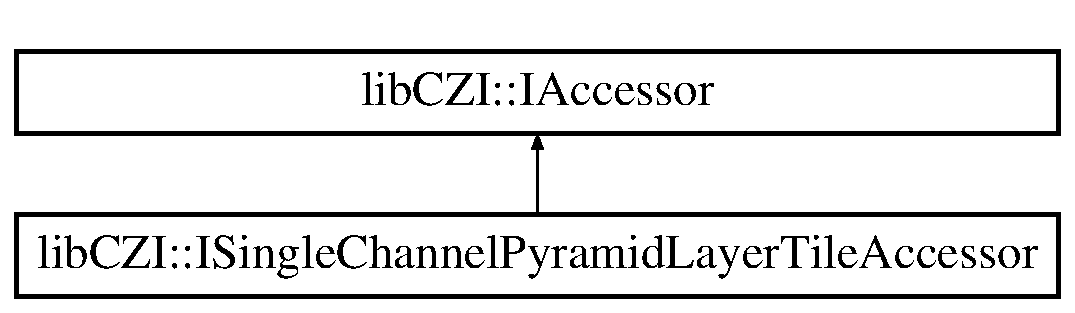
\includegraphics[height=2.000000cm]{classlib_c_z_i_1_1_i_single_channel_pyramid_layer_tile_accessor}
\end{center}
\end{figure}
\subsection*{Classes}
\begin{DoxyCompactItemize}
\item 
struct \hyperlink{structlib_c_z_i_1_1_i_single_channel_pyramid_layer_tile_accessor_1_1_options}{Options}
\begin{DoxyCompactList}\small\item\em \hyperlink{structlib_c_z_i_1_1_i_single_channel_pyramid_layer_tile_accessor_1_1_options}{Options} used for this accessor. \end{DoxyCompactList}\item 
struct \hyperlink{structlib_c_z_i_1_1_i_single_channel_pyramid_layer_tile_accessor_1_1_pyramid_layer_info}{Pyramid\+Layer\+Info}
\end{DoxyCompactItemize}
\subsection*{Public Member Functions}
\begin{DoxyCompactItemize}
\item 
virtual std\+::shared\+\_\+ptr$<$ \hyperlink{classlib_c_z_i_1_1_i_bitmap_data}{lib\+C\+Z\+I\+::\+I\+Bitmap\+Data} $>$ \hyperlink{classlib_c_z_i_1_1_i_single_channel_pyramid_layer_tile_accessor_ac4dd5b960114aa8f87773734d9d78dd3}{Get} (const \hyperlink{structlib_c_z_i_1_1_int_rect}{lib\+C\+Z\+I\+::\+Int\+Rect} \&roi, const \hyperlink{classlib_c_z_i_1_1_i_dim_coordinate}{lib\+C\+Z\+I\+::\+I\+Dim\+Coordinate} $\ast$plane\+Coordinate, const \hyperlink{structlib_c_z_i_1_1_i_single_channel_pyramid_layer_tile_accessor_1_1_pyramid_layer_info}{Pyramid\+Layer\+Info} \&pyramid\+Info, const \hyperlink{structlib_c_z_i_1_1_i_single_channel_pyramid_layer_tile_accessor_1_1_options}{lib\+C\+Z\+I\+::\+I\+Single\+Channel\+Pyramid\+Layer\+Tile\+Accessor\+::\+Options} $\ast$p\+Options)=0
\item 
virtual std\+::shared\+\_\+ptr$<$ \hyperlink{classlib_c_z_i_1_1_i_bitmap_data}{lib\+C\+Z\+I\+::\+I\+Bitmap\+Data} $>$ \hyperlink{classlib_c_z_i_1_1_i_single_channel_pyramid_layer_tile_accessor_a089932803187582a1c19b39b45694fd7}{Get} (\hyperlink{namespacelib_c_z_i_abf8ce12ab88b06c8b3b47efbb5e2e834}{lib\+C\+Z\+I\+::\+Pixel\+Type} pixeltype, const \hyperlink{structlib_c_z_i_1_1_int_rect}{lib\+C\+Z\+I\+::\+Int\+Rect} \&roi, const \hyperlink{classlib_c_z_i_1_1_i_dim_coordinate}{lib\+C\+Z\+I\+::\+I\+Dim\+Coordinate} $\ast$plane\+Coordinate, const \hyperlink{structlib_c_z_i_1_1_i_single_channel_pyramid_layer_tile_accessor_1_1_pyramid_layer_info}{Pyramid\+Layer\+Info} \&pyramid\+Info, const \hyperlink{structlib_c_z_i_1_1_i_single_channel_pyramid_layer_tile_accessor_1_1_options}{lib\+C\+Z\+I\+::\+I\+Single\+Channel\+Pyramid\+Layer\+Tile\+Accessor\+::\+Options} $\ast$p\+Options)=0
\item 
virtual void \hyperlink{classlib_c_z_i_1_1_i_single_channel_pyramid_layer_tile_accessor_a0aff0f380ba7819cf5a4cc239ff7579f}{Get} (\hyperlink{classlib_c_z_i_1_1_i_bitmap_data}{lib\+C\+Z\+I\+::\+I\+Bitmap\+Data} $\ast$p\+Dest, int x\+Pos, int y\+Pos, const \hyperlink{classlib_c_z_i_1_1_i_dim_coordinate}{I\+Dim\+Coordinate} $\ast$plane\+Coordinate, const \hyperlink{structlib_c_z_i_1_1_i_single_channel_pyramid_layer_tile_accessor_1_1_pyramid_layer_info}{Pyramid\+Layer\+Info} \&pyramid\+Info, const \hyperlink{structlib_c_z_i_1_1_i_single_channel_pyramid_layer_tile_accessor_1_1_options}{Options} $\ast$p\+Options)=0
\begin{DoxyCompactList}\small\item\em Copy the composite to the specified bitmap. \end{DoxyCompactList}\end{DoxyCompactItemize}


\subsection{Detailed Description}
Interface for single-\/channel-\/pyramidlayer tile accessors. It allows to directly address the pyramid-\/layer it operates on. This accessor creates a multi-\/tile composite of a single channel (and a single plane) from a specified pyramid-\/layer. 

\subsection{Member Function Documentation}
\mbox{\Hypertarget{classlib_c_z_i_1_1_i_single_channel_pyramid_layer_tile_accessor_ac4dd5b960114aa8f87773734d9d78dd3}\label{classlib_c_z_i_1_1_i_single_channel_pyramid_layer_tile_accessor_ac4dd5b960114aa8f87773734d9d78dd3}} 
\index{lib\+C\+Z\+I\+::\+I\+Single\+Channel\+Pyramid\+Layer\+Tile\+Accessor@{lib\+C\+Z\+I\+::\+I\+Single\+Channel\+Pyramid\+Layer\+Tile\+Accessor}!Get@{Get}}
\index{Get@{Get}!lib\+C\+Z\+I\+::\+I\+Single\+Channel\+Pyramid\+Layer\+Tile\+Accessor@{lib\+C\+Z\+I\+::\+I\+Single\+Channel\+Pyramid\+Layer\+Tile\+Accessor}}
\subsubsection{\texorpdfstring{Get()}{Get()}\hspace{0.1cm}{\footnotesize\ttfamily [1/3]}}
{\footnotesize\ttfamily virtual std\+::shared\+\_\+ptr$<$\hyperlink{classlib_c_z_i_1_1_i_bitmap_data}{lib\+C\+Z\+I\+::\+I\+Bitmap\+Data}$>$ lib\+C\+Z\+I\+::\+I\+Single\+Channel\+Pyramid\+Layer\+Tile\+Accessor\+::\+Get (\begin{DoxyParamCaption}\item[{const \hyperlink{structlib_c_z_i_1_1_int_rect}{lib\+C\+Z\+I\+::\+Int\+Rect} \&}]{roi,  }\item[{const \hyperlink{classlib_c_z_i_1_1_i_dim_coordinate}{lib\+C\+Z\+I\+::\+I\+Dim\+Coordinate} $\ast$}]{plane\+Coordinate,  }\item[{const \hyperlink{structlib_c_z_i_1_1_i_single_channel_pyramid_layer_tile_accessor_1_1_pyramid_layer_info}{Pyramid\+Layer\+Info} \&}]{pyramid\+Info,  }\item[{const \hyperlink{structlib_c_z_i_1_1_i_single_channel_pyramid_layer_tile_accessor_1_1_options}{lib\+C\+Z\+I\+::\+I\+Single\+Channel\+Pyramid\+Layer\+Tile\+Accessor\+::\+Options} $\ast$}]{p\+Options }\end{DoxyParamCaption})\hspace{0.3cm}{\ttfamily [pure virtual]}}

Gets the tile composite of the specified plane and the specified R\+OI and the specified pyramid-\/layer. The pixeltype is determined by examing the first subblock found in the specified plane (which is an arbitrary subblock). A newly allocated bitmap is returned. 
\begin{DoxyParams}{Parameters}
{\em roi} & The R\+OI. \\
\hline
{\em plane\+Coordinate} & The plane coordinate. \\
\hline
{\em pyramid\+Info} & Information describing the pyramid-\/layer. \\
\hline
{\em p\+Options} & \hyperlink{structlib_c_z_i_1_1_i_single_channel_pyramid_layer_tile_accessor_1_1_options}{Options} for controlling the operation. \\
\hline
\end{DoxyParams}
\begin{DoxyReturn}{Returns}
A std\+::shared\+\_\+ptr$<$\hyperlink{classlib_c_z_i_1_1_i_bitmap_data}{lib\+C\+Z\+I\+::\+I\+Bitmap\+Data}$>$ 
\end{DoxyReturn}
\mbox{\Hypertarget{classlib_c_z_i_1_1_i_single_channel_pyramid_layer_tile_accessor_a089932803187582a1c19b39b45694fd7}\label{classlib_c_z_i_1_1_i_single_channel_pyramid_layer_tile_accessor_a089932803187582a1c19b39b45694fd7}} 
\index{lib\+C\+Z\+I\+::\+I\+Single\+Channel\+Pyramid\+Layer\+Tile\+Accessor@{lib\+C\+Z\+I\+::\+I\+Single\+Channel\+Pyramid\+Layer\+Tile\+Accessor}!Get@{Get}}
\index{Get@{Get}!lib\+C\+Z\+I\+::\+I\+Single\+Channel\+Pyramid\+Layer\+Tile\+Accessor@{lib\+C\+Z\+I\+::\+I\+Single\+Channel\+Pyramid\+Layer\+Tile\+Accessor}}
\subsubsection{\texorpdfstring{Get()}{Get()}\hspace{0.1cm}{\footnotesize\ttfamily [2/3]}}
{\footnotesize\ttfamily virtual std\+::shared\+\_\+ptr$<$\hyperlink{classlib_c_z_i_1_1_i_bitmap_data}{lib\+C\+Z\+I\+::\+I\+Bitmap\+Data}$>$ lib\+C\+Z\+I\+::\+I\+Single\+Channel\+Pyramid\+Layer\+Tile\+Accessor\+::\+Get (\begin{DoxyParamCaption}\item[{\hyperlink{namespacelib_c_z_i_abf8ce12ab88b06c8b3b47efbb5e2e834}{lib\+C\+Z\+I\+::\+Pixel\+Type}}]{pixeltype,  }\item[{const \hyperlink{structlib_c_z_i_1_1_int_rect}{lib\+C\+Z\+I\+::\+Int\+Rect} \&}]{roi,  }\item[{const \hyperlink{classlib_c_z_i_1_1_i_dim_coordinate}{lib\+C\+Z\+I\+::\+I\+Dim\+Coordinate} $\ast$}]{plane\+Coordinate,  }\item[{const \hyperlink{structlib_c_z_i_1_1_i_single_channel_pyramid_layer_tile_accessor_1_1_pyramid_layer_info}{Pyramid\+Layer\+Info} \&}]{pyramid\+Info,  }\item[{const \hyperlink{structlib_c_z_i_1_1_i_single_channel_pyramid_layer_tile_accessor_1_1_options}{lib\+C\+Z\+I\+::\+I\+Single\+Channel\+Pyramid\+Layer\+Tile\+Accessor\+::\+Options} $\ast$}]{p\+Options }\end{DoxyParamCaption})\hspace{0.3cm}{\ttfamily [pure virtual]}}

Gets the tile composite of the specified plane and the specified R\+OI and the specified pyramid-\/layer. 
\begin{DoxyParams}{Parameters}
{\em pixeltype} & The pixeltype (of the destination bitmap). \\
\hline
{\em roi} & The R\+OI. \\
\hline
{\em plane\+Coordinate} & The plane coordinate. \\
\hline
{\em pyramid\+Info} & Information describing the pyramid-\/layer. \\
\hline
{\em p\+Options} & \hyperlink{structlib_c_z_i_1_1_i_single_channel_pyramid_layer_tile_accessor_1_1_options}{Options} for controlling the operation. \\
\hline
\end{DoxyParams}
\begin{DoxyReturn}{Returns}
A std\+::shared\+\_\+ptr$<$\hyperlink{classlib_c_z_i_1_1_i_bitmap_data}{lib\+C\+Z\+I\+::\+I\+Bitmap\+Data}$>$ 
\end{DoxyReturn}
\mbox{\Hypertarget{classlib_c_z_i_1_1_i_single_channel_pyramid_layer_tile_accessor_a0aff0f380ba7819cf5a4cc239ff7579f}\label{classlib_c_z_i_1_1_i_single_channel_pyramid_layer_tile_accessor_a0aff0f380ba7819cf5a4cc239ff7579f}} 
\index{lib\+C\+Z\+I\+::\+I\+Single\+Channel\+Pyramid\+Layer\+Tile\+Accessor@{lib\+C\+Z\+I\+::\+I\+Single\+Channel\+Pyramid\+Layer\+Tile\+Accessor}!Get@{Get}}
\index{Get@{Get}!lib\+C\+Z\+I\+::\+I\+Single\+Channel\+Pyramid\+Layer\+Tile\+Accessor@{lib\+C\+Z\+I\+::\+I\+Single\+Channel\+Pyramid\+Layer\+Tile\+Accessor}}
\subsubsection{\texorpdfstring{Get()}{Get()}\hspace{0.1cm}{\footnotesize\ttfamily [3/3]}}
{\footnotesize\ttfamily virtual void lib\+C\+Z\+I\+::\+I\+Single\+Channel\+Pyramid\+Layer\+Tile\+Accessor\+::\+Get (\begin{DoxyParamCaption}\item[{\hyperlink{classlib_c_z_i_1_1_i_bitmap_data}{lib\+C\+Z\+I\+::\+I\+Bitmap\+Data} $\ast$}]{p\+Dest,  }\item[{int}]{x\+Pos,  }\item[{int}]{y\+Pos,  }\item[{const \hyperlink{classlib_c_z_i_1_1_i_dim_coordinate}{I\+Dim\+Coordinate} $\ast$}]{plane\+Coordinate,  }\item[{const \hyperlink{structlib_c_z_i_1_1_i_single_channel_pyramid_layer_tile_accessor_1_1_pyramid_layer_info}{Pyramid\+Layer\+Info} \&}]{pyramid\+Info,  }\item[{const \hyperlink{structlib_c_z_i_1_1_i_single_channel_pyramid_layer_tile_accessor_1_1_options}{Options} $\ast$}]{p\+Options }\end{DoxyParamCaption})\hspace{0.3cm}{\ttfamily [pure virtual]}}



Copy the composite to the specified bitmap. 


\begin{DoxyParams}[1]{Parameters}
\mbox{\tt out}  & {\em p\+Dest} & The destination bitmap (also defining the width and height) \\
\hline
 & {\em x\+Pos} & The x-\/position. \\
\hline
 & {\em y\+Pos} & The y-\/position. \\
\hline
 & {\em plane\+Coordinate} & The plane coordinate. \\
\hline
 & {\em pyramid\+Info} & Information describing the pyramid-\/layer. \\
\hline
 & {\em p\+Options} & \hyperlink{structlib_c_z_i_1_1_i_single_channel_pyramid_layer_tile_accessor_1_1_options}{Options} for controlling the operation. \\
\hline
\end{DoxyParams}


The documentation for this class was generated from the following file\+:\begin{DoxyCompactItemize}
\item 
lib\+C\+Z\+I/lib\+C\+Z\+I\+\_\+\+Compositor.\+h\end{DoxyCompactItemize}

\hypertarget{classlib_c_z_i_1_1_i_single_channel_scaling_tile_accessor}{}\section{lib\+C\+ZI\+:\+:I\+Single\+Channel\+Scaling\+Tile\+Accessor Class Reference}
\label{classlib_c_z_i_1_1_i_single_channel_scaling_tile_accessor}\index{lib\+C\+Z\+I\+::\+I\+Single\+Channel\+Scaling\+Tile\+Accessor@{lib\+C\+Z\+I\+::\+I\+Single\+Channel\+Scaling\+Tile\+Accessor}}


{\ttfamily \#include $<$lib\+C\+Z\+I\+\_\+\+Compositor.\+h$>$}

Inheritance diagram for lib\+C\+ZI\+:\+:I\+Single\+Channel\+Scaling\+Tile\+Accessor\+:\begin{figure}[H]
\begin{center}
\leavevmode
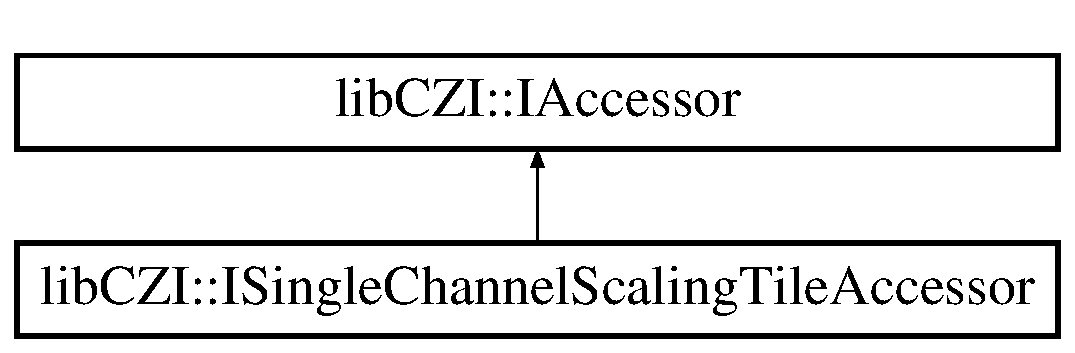
\includegraphics[height=2.000000cm]{classlib_c_z_i_1_1_i_single_channel_scaling_tile_accessor}
\end{center}
\end{figure}
\subsection*{Classes}
\begin{DoxyCompactItemize}
\item 
struct \hyperlink{structlib_c_z_i_1_1_i_single_channel_scaling_tile_accessor_1_1_options}{Options}
\begin{DoxyCompactList}\small\item\em \hyperlink{structlib_c_z_i_1_1_i_single_channel_scaling_tile_accessor_1_1_options}{Options} used for this accessor. \end{DoxyCompactList}\end{DoxyCompactItemize}
\subsection*{Public Member Functions}
\begin{DoxyCompactItemize}
\item 
virtual \hyperlink{structlib_c_z_i_1_1_int_size}{lib\+C\+Z\+I\+::\+Int\+Size} \hyperlink{classlib_c_z_i_1_1_i_single_channel_scaling_tile_accessor_aa7a0c9edcdd3460471edfdbe54fc2f76}{Calc\+Size} (const \hyperlink{structlib_c_z_i_1_1_int_rect}{lib\+C\+Z\+I\+::\+Int\+Rect} \&roi, float zoom) const =0
\item 
virtual std\+::shared\+\_\+ptr$<$ \hyperlink{classlib_c_z_i_1_1_i_bitmap_data}{lib\+C\+Z\+I\+::\+I\+Bitmap\+Data} $>$ \hyperlink{classlib_c_z_i_1_1_i_single_channel_scaling_tile_accessor_a3cd342d241a2c438a0b71d1342428a58}{Get} (const \hyperlink{structlib_c_z_i_1_1_int_rect}{lib\+C\+Z\+I\+::\+Int\+Rect} \&roi, const \hyperlink{classlib_c_z_i_1_1_i_dim_coordinate}{lib\+C\+Z\+I\+::\+I\+Dim\+Coordinate} $\ast$plane\+Coordinate, float zoom, const \hyperlink{structlib_c_z_i_1_1_i_single_channel_scaling_tile_accessor_1_1_options}{lib\+C\+Z\+I\+::\+I\+Single\+Channel\+Scaling\+Tile\+Accessor\+::\+Options} $\ast$p\+Options)=0
\item 
virtual std\+::shared\+\_\+ptr$<$ \hyperlink{classlib_c_z_i_1_1_i_bitmap_data}{lib\+C\+Z\+I\+::\+I\+Bitmap\+Data} $>$ \hyperlink{classlib_c_z_i_1_1_i_single_channel_scaling_tile_accessor_a1cd1fe10e445d286f4c64b75d4734caf}{Get} (\hyperlink{namespacelib_c_z_i_abf8ce12ab88b06c8b3b47efbb5e2e834}{lib\+C\+Z\+I\+::\+Pixel\+Type} pixeltype, const \hyperlink{structlib_c_z_i_1_1_int_rect}{lib\+C\+Z\+I\+::\+Int\+Rect} \&roi, const \hyperlink{classlib_c_z_i_1_1_i_dim_coordinate}{lib\+C\+Z\+I\+::\+I\+Dim\+Coordinate} $\ast$plane\+Coordinate, float zoom, const \hyperlink{structlib_c_z_i_1_1_i_single_channel_scaling_tile_accessor_1_1_options}{lib\+C\+Z\+I\+::\+I\+Single\+Channel\+Scaling\+Tile\+Accessor\+::\+Options} $\ast$p\+Options)=0
\item 
virtual void \hyperlink{classlib_c_z_i_1_1_i_single_channel_scaling_tile_accessor_a09a7963766e4c99721e6c3e13dca61cb}{Get} (\hyperlink{classlib_c_z_i_1_1_i_bitmap_data}{lib\+C\+Z\+I\+::\+I\+Bitmap\+Data} $\ast$p\+Dest, const \hyperlink{structlib_c_z_i_1_1_int_rect}{lib\+C\+Z\+I\+::\+Int\+Rect} \&roi, const \hyperlink{classlib_c_z_i_1_1_i_dim_coordinate}{lib\+C\+Z\+I\+::\+I\+Dim\+Coordinate} $\ast$plane\+Coordinate, float zoom, const \hyperlink{structlib_c_z_i_1_1_i_single_channel_scaling_tile_accessor_1_1_options}{lib\+C\+Z\+I\+::\+I\+Single\+Channel\+Scaling\+Tile\+Accessor\+::\+Options} $\ast$p\+Options)=0
\begin{DoxyCompactList}\small\item\em Copy the composite to the specified bitmap. \end{DoxyCompactList}\end{DoxyCompactItemize}


\subsection{Detailed Description}
Interface for single channel scaling tile accessors. This accessor creates a multi-\/tile composite of a single channel (and a single plane) with a given zoom-\/factor. It will use pyramid sub-\/blocks (if present) in order to create the destination bitmap. In this operation, it will use the pyramid-\/layer just above the specified zoom-\/factor and scale down to the requested size.~\newline
The scaling operation employed here is a simple nearest-\/neighbor algorithm. 

\subsection{Member Function Documentation}
\mbox{\Hypertarget{classlib_c_z_i_1_1_i_single_channel_scaling_tile_accessor_aa7a0c9edcdd3460471edfdbe54fc2f76}\label{classlib_c_z_i_1_1_i_single_channel_scaling_tile_accessor_aa7a0c9edcdd3460471edfdbe54fc2f76}} 
\index{lib\+C\+Z\+I\+::\+I\+Single\+Channel\+Scaling\+Tile\+Accessor@{lib\+C\+Z\+I\+::\+I\+Single\+Channel\+Scaling\+Tile\+Accessor}!Calc\+Size@{Calc\+Size}}
\index{Calc\+Size@{Calc\+Size}!lib\+C\+Z\+I\+::\+I\+Single\+Channel\+Scaling\+Tile\+Accessor@{lib\+C\+Z\+I\+::\+I\+Single\+Channel\+Scaling\+Tile\+Accessor}}
\subsubsection{\texorpdfstring{Calc\+Size()}{CalcSize()}}
{\footnotesize\ttfamily virtual \hyperlink{structlib_c_z_i_1_1_int_size}{lib\+C\+Z\+I\+::\+Int\+Size} lib\+C\+Z\+I\+::\+I\+Single\+Channel\+Scaling\+Tile\+Accessor\+::\+Calc\+Size (\begin{DoxyParamCaption}\item[{const \hyperlink{structlib_c_z_i_1_1_int_rect}{lib\+C\+Z\+I\+::\+Int\+Rect} \&}]{roi,  }\item[{float}]{zoom }\end{DoxyParamCaption}) const\hspace{0.3cm}{\ttfamily [pure virtual]}}

Calculates the size a bitmap will have (when created by this accessor) for the specified R\+OI and the specified Zoom. Since the exact size if subject to rounding errors, one should always use this method if the exact size must be known beforehand. The Get-\/method which operates on a pre-\/allocated bitmap will only work if the size (of the bitmap passed in) exactly matches. 
\begin{DoxyParams}{Parameters}
{\em roi} & The R\+OI. \\
\hline
{\em zoom} & The zoom factor. \\
\hline
\end{DoxyParams}
\begin{DoxyReturn}{Returns}
The size of the composite created by this accessor (for these parameters). 
\end{DoxyReturn}
\mbox{\Hypertarget{classlib_c_z_i_1_1_i_single_channel_scaling_tile_accessor_a3cd342d241a2c438a0b71d1342428a58}\label{classlib_c_z_i_1_1_i_single_channel_scaling_tile_accessor_a3cd342d241a2c438a0b71d1342428a58}} 
\index{lib\+C\+Z\+I\+::\+I\+Single\+Channel\+Scaling\+Tile\+Accessor@{lib\+C\+Z\+I\+::\+I\+Single\+Channel\+Scaling\+Tile\+Accessor}!Get@{Get}}
\index{Get@{Get}!lib\+C\+Z\+I\+::\+I\+Single\+Channel\+Scaling\+Tile\+Accessor@{lib\+C\+Z\+I\+::\+I\+Single\+Channel\+Scaling\+Tile\+Accessor}}
\subsubsection{\texorpdfstring{Get()}{Get()}\hspace{0.1cm}{\footnotesize\ttfamily [1/3]}}
{\footnotesize\ttfamily virtual std\+::shared\+\_\+ptr$<$\hyperlink{classlib_c_z_i_1_1_i_bitmap_data}{lib\+C\+Z\+I\+::\+I\+Bitmap\+Data}$>$ lib\+C\+Z\+I\+::\+I\+Single\+Channel\+Scaling\+Tile\+Accessor\+::\+Get (\begin{DoxyParamCaption}\item[{const \hyperlink{structlib_c_z_i_1_1_int_rect}{lib\+C\+Z\+I\+::\+Int\+Rect} \&}]{roi,  }\item[{const \hyperlink{classlib_c_z_i_1_1_i_dim_coordinate}{lib\+C\+Z\+I\+::\+I\+Dim\+Coordinate} $\ast$}]{plane\+Coordinate,  }\item[{float}]{zoom,  }\item[{const \hyperlink{structlib_c_z_i_1_1_i_single_channel_scaling_tile_accessor_1_1_options}{lib\+C\+Z\+I\+::\+I\+Single\+Channel\+Scaling\+Tile\+Accessor\+::\+Options} $\ast$}]{p\+Options }\end{DoxyParamCaption})\hspace{0.3cm}{\ttfamily [pure virtual]}}

Gets the scaled tile composite of the specified plane and the specified R\+OI with the specifed zoom factor.~\newline
The pixeltype is determined by examing the first subblock found in the specified plane (which is an arbitrary subblock). A newly allocated bitmap is returned. 
\begin{DoxyParams}{Parameters}
{\em roi} & The R\+OI. \\
\hline
{\em plane\+Coordinate} & The plane coordinate. \\
\hline
{\em zoom} & The zoom. \\
\hline
{\em p\+Options} & \hyperlink{structlib_c_z_i_1_1_i_single_channel_scaling_tile_accessor_1_1_options}{Options} for controlling the operation (may be nullptr). \\
\hline
\end{DoxyParams}
\begin{DoxyReturn}{Returns}
A std\+::shared\+\_\+ptr$<$\hyperlink{classlib_c_z_i_1_1_i_bitmap_data}{lib\+C\+Z\+I\+::\+I\+Bitmap\+Data}$>$ 
\end{DoxyReturn}
\mbox{\Hypertarget{classlib_c_z_i_1_1_i_single_channel_scaling_tile_accessor_a1cd1fe10e445d286f4c64b75d4734caf}\label{classlib_c_z_i_1_1_i_single_channel_scaling_tile_accessor_a1cd1fe10e445d286f4c64b75d4734caf}} 
\index{lib\+C\+Z\+I\+::\+I\+Single\+Channel\+Scaling\+Tile\+Accessor@{lib\+C\+Z\+I\+::\+I\+Single\+Channel\+Scaling\+Tile\+Accessor}!Get@{Get}}
\index{Get@{Get}!lib\+C\+Z\+I\+::\+I\+Single\+Channel\+Scaling\+Tile\+Accessor@{lib\+C\+Z\+I\+::\+I\+Single\+Channel\+Scaling\+Tile\+Accessor}}
\subsubsection{\texorpdfstring{Get()}{Get()}\hspace{0.1cm}{\footnotesize\ttfamily [2/3]}}
{\footnotesize\ttfamily virtual std\+::shared\+\_\+ptr$<$\hyperlink{classlib_c_z_i_1_1_i_bitmap_data}{lib\+C\+Z\+I\+::\+I\+Bitmap\+Data}$>$ lib\+C\+Z\+I\+::\+I\+Single\+Channel\+Scaling\+Tile\+Accessor\+::\+Get (\begin{DoxyParamCaption}\item[{\hyperlink{namespacelib_c_z_i_abf8ce12ab88b06c8b3b47efbb5e2e834}{lib\+C\+Z\+I\+::\+Pixel\+Type}}]{pixeltype,  }\item[{const \hyperlink{structlib_c_z_i_1_1_int_rect}{lib\+C\+Z\+I\+::\+Int\+Rect} \&}]{roi,  }\item[{const \hyperlink{classlib_c_z_i_1_1_i_dim_coordinate}{lib\+C\+Z\+I\+::\+I\+Dim\+Coordinate} $\ast$}]{plane\+Coordinate,  }\item[{float}]{zoom,  }\item[{const \hyperlink{structlib_c_z_i_1_1_i_single_channel_scaling_tile_accessor_1_1_options}{lib\+C\+Z\+I\+::\+I\+Single\+Channel\+Scaling\+Tile\+Accessor\+::\+Options} $\ast$}]{p\+Options }\end{DoxyParamCaption})\hspace{0.3cm}{\ttfamily [pure virtual]}}

Gets the scaled tile composite of the specified plane and the specified R\+OI with the specifed zoom factor. 
\begin{DoxyParams}{Parameters}
{\em pixeltype} & The pixeltype (of the destination bitmap). \\
\hline
{\em roi} & The R\+OI. \\
\hline
{\em plane\+Coordinate} & The plane coordinate. \\
\hline
{\em zoom} & The zoom factor. \\
\hline
{\em p\+Options} & \hyperlink{structlib_c_z_i_1_1_i_single_channel_scaling_tile_accessor_1_1_options}{Options} for controlling the operation (may be nullptr). \\
\hline
\end{DoxyParams}
\begin{DoxyReturn}{Returns}
A std\+::shared\+\_\+ptr$<$\hyperlink{classlib_c_z_i_1_1_i_bitmap_data}{lib\+C\+Z\+I\+::\+I\+Bitmap\+Data}$>$ 
\end{DoxyReturn}
\mbox{\Hypertarget{classlib_c_z_i_1_1_i_single_channel_scaling_tile_accessor_a09a7963766e4c99721e6c3e13dca61cb}\label{classlib_c_z_i_1_1_i_single_channel_scaling_tile_accessor_a09a7963766e4c99721e6c3e13dca61cb}} 
\index{lib\+C\+Z\+I\+::\+I\+Single\+Channel\+Scaling\+Tile\+Accessor@{lib\+C\+Z\+I\+::\+I\+Single\+Channel\+Scaling\+Tile\+Accessor}!Get@{Get}}
\index{Get@{Get}!lib\+C\+Z\+I\+::\+I\+Single\+Channel\+Scaling\+Tile\+Accessor@{lib\+C\+Z\+I\+::\+I\+Single\+Channel\+Scaling\+Tile\+Accessor}}
\subsubsection{\texorpdfstring{Get()}{Get()}\hspace{0.1cm}{\footnotesize\ttfamily [3/3]}}
{\footnotesize\ttfamily virtual void lib\+C\+Z\+I\+::\+I\+Single\+Channel\+Scaling\+Tile\+Accessor\+::\+Get (\begin{DoxyParamCaption}\item[{\hyperlink{classlib_c_z_i_1_1_i_bitmap_data}{lib\+C\+Z\+I\+::\+I\+Bitmap\+Data} $\ast$}]{p\+Dest,  }\item[{const \hyperlink{structlib_c_z_i_1_1_int_rect}{lib\+C\+Z\+I\+::\+Int\+Rect} \&}]{roi,  }\item[{const \hyperlink{classlib_c_z_i_1_1_i_dim_coordinate}{lib\+C\+Z\+I\+::\+I\+Dim\+Coordinate} $\ast$}]{plane\+Coordinate,  }\item[{float}]{zoom,  }\item[{const \hyperlink{structlib_c_z_i_1_1_i_single_channel_scaling_tile_accessor_1_1_options}{lib\+C\+Z\+I\+::\+I\+Single\+Channel\+Scaling\+Tile\+Accessor\+::\+Options} $\ast$}]{p\+Options }\end{DoxyParamCaption})\hspace{0.3cm}{\ttfamily [pure virtual]}}



Copy the composite to the specified bitmap. 

The size of the bitmap must exactly match the size reported by the method \char`\"{}\+Calc\+Size\char`\"{} (for the same R\+OI and zoom), otherwise an invalid\+\_\+argument-\/exception is thrown. 


\begin{DoxyParams}{Parameters}
{\em p\+Dest} & \mbox{[}in,out\mbox{]} The destination bitmap. \\
\hline
{\em roi} & The R\+OI. \\
\hline
{\em plane\+Coordinate} & The plane coordinate. \\
\hline
{\em zoom} & The zoom factor. \\
\hline
{\em p\+Options} & \hyperlink{structlib_c_z_i_1_1_i_single_channel_scaling_tile_accessor_1_1_options}{Options} controlling the operation. May be nullptr.\\
\hline
\end{DoxyParams}


The documentation for this class was generated from the following file\+:\begin{DoxyCompactItemize}
\item 
lib\+C\+Z\+I/lib\+C\+Z\+I\+\_\+\+Compositor.\+h\end{DoxyCompactItemize}

\hypertarget{classlib_c_z_i_1_1_i_single_channel_tile_accessor}{}\section{lib\+C\+ZI\+:\+:I\+Single\+Channel\+Tile\+Accessor Class Reference}
\label{classlib_c_z_i_1_1_i_single_channel_tile_accessor}\index{lib\+C\+Z\+I\+::\+I\+Single\+Channel\+Tile\+Accessor@{lib\+C\+Z\+I\+::\+I\+Single\+Channel\+Tile\+Accessor}}


{\ttfamily \#include $<$lib\+C\+Z\+I\+\_\+\+Compositor.\+h$>$}

Inheritance diagram for lib\+C\+ZI\+:\+:I\+Single\+Channel\+Tile\+Accessor\+:\begin{figure}[H]
\begin{center}
\leavevmode
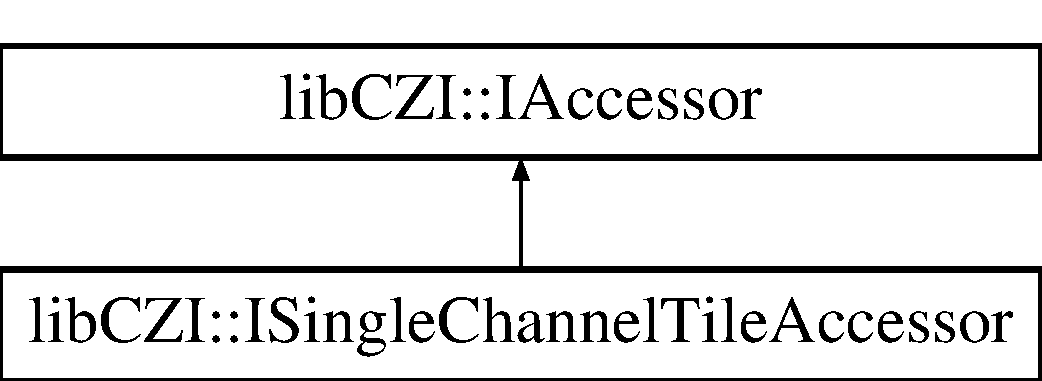
\includegraphics[height=2.000000cm]{classlib_c_z_i_1_1_i_single_channel_tile_accessor}
\end{center}
\end{figure}
\subsection*{Classes}
\begin{DoxyCompactItemize}
\item 
struct \hyperlink{structlib_c_z_i_1_1_i_single_channel_tile_accessor_1_1_options}{Options}
\begin{DoxyCompactList}\small\item\em \hyperlink{structlib_c_z_i_1_1_i_single_channel_tile_accessor_1_1_options}{Options} for controlling the composition operation. \end{DoxyCompactList}\end{DoxyCompactItemize}
\subsection*{Public Member Functions}
\begin{DoxyCompactItemize}
\item 
virtual std\+::shared\+\_\+ptr$<$ \hyperlink{classlib_c_z_i_1_1_i_bitmap_data}{lib\+C\+Z\+I\+::\+I\+Bitmap\+Data} $>$ \hyperlink{classlib_c_z_i_1_1_i_single_channel_tile_accessor_a50e17c0c197bf5f782a67e044dd4e943}{Get} (const \hyperlink{structlib_c_z_i_1_1_int_rect}{lib\+C\+Z\+I\+::\+Int\+Rect} \&roi, const \hyperlink{classlib_c_z_i_1_1_i_dim_coordinate}{I\+Dim\+Coordinate} $\ast$plane\+Coordinate, const \hyperlink{structlib_c_z_i_1_1_i_single_channel_tile_accessor_1_1_options}{Options} $\ast$p\+Options)=0
\begin{DoxyCompactList}\small\item\em Gets the tile composite of the specified plane and the specified R\+OI. The pixeltype is determined by examing the first subblock found in the specified plane (which is an arbitrary subblock). A newly allocated bitmap is returned. \end{DoxyCompactList}\item 
virtual std\+::shared\+\_\+ptr$<$ \hyperlink{classlib_c_z_i_1_1_i_bitmap_data}{lib\+C\+Z\+I\+::\+I\+Bitmap\+Data} $>$ \hyperlink{classlib_c_z_i_1_1_i_single_channel_tile_accessor_a4fb81512693a2d7221abece14c33d1f3}{Get} (\hyperlink{namespacelib_c_z_i_abf8ce12ab88b06c8b3b47efbb5e2e834}{lib\+C\+Z\+I\+::\+Pixel\+Type} pixeltype, const \hyperlink{structlib_c_z_i_1_1_int_rect}{lib\+C\+Z\+I\+::\+Int\+Rect} \&roi, const \hyperlink{classlib_c_z_i_1_1_i_dim_coordinate}{I\+Dim\+Coordinate} $\ast$plane\+Coordinate, const \hyperlink{structlib_c_z_i_1_1_i_single_channel_tile_accessor_1_1_options}{Options} $\ast$p\+Options)=0
\item 
virtual void \hyperlink{classlib_c_z_i_1_1_i_single_channel_tile_accessor_a275295786554ca6dbf9f2d0b3086dcad}{Get} (\hyperlink{classlib_c_z_i_1_1_i_bitmap_data}{lib\+C\+Z\+I\+::\+I\+Bitmap\+Data} $\ast$p\+Dest, int x\+Pos, int y\+Pos, const \hyperlink{classlib_c_z_i_1_1_i_dim_coordinate}{I\+Dim\+Coordinate} $\ast$plane\+Coordinate, const \hyperlink{structlib_c_z_i_1_1_i_single_channel_tile_accessor_1_1_options}{Options} $\ast$p\+Options)=0
\item 
std\+::shared\+\_\+ptr$<$ \hyperlink{classlib_c_z_i_1_1_i_bitmap_data}{lib\+C\+Z\+I\+::\+I\+Bitmap\+Data} $>$ \hyperlink{classlib_c_z_i_1_1_i_single_channel_tile_accessor_a9ef98a25e06e5da36d811705bb076dcc}{Get} (int x\+Pos, int y\+Pos, int width, int height, const \hyperlink{classlib_c_z_i_1_1_i_dim_coordinate}{I\+Dim\+Coordinate} $\ast$plane\+Coordinate, const \hyperlink{structlib_c_z_i_1_1_i_single_channel_tile_accessor_1_1_options}{Options} $\ast$p\+Options)
\item 
std\+::shared\+\_\+ptr$<$ \hyperlink{classlib_c_z_i_1_1_i_bitmap_data}{lib\+C\+Z\+I\+::\+I\+Bitmap\+Data} $>$ \hyperlink{classlib_c_z_i_1_1_i_single_channel_tile_accessor_a8a9654ed1df4929068477a43597bf084}{Get} (\hyperlink{namespacelib_c_z_i_abf8ce12ab88b06c8b3b47efbb5e2e834}{lib\+C\+Z\+I\+::\+Pixel\+Type} pixeltype, int x\+Pos, int y\+Pos, int width, int height, const \hyperlink{classlib_c_z_i_1_1_i_dim_coordinate}{I\+Dim\+Coordinate} $\ast$plane\+Coordinate, const \hyperlink{structlib_c_z_i_1_1_i_single_channel_tile_accessor_1_1_options}{Options} $\ast$p\+Options)
\end{DoxyCompactItemize}


\subsection{Detailed Description}
This accessor creates a multi-\/tile composite of a single channel (and a single plane). The accessor will request all tiles that intersect with the specified R\+OI and are on the specified plane and create a composite as shown here\+:  
\begin{DoxyImageNoCaption}
  \mbox{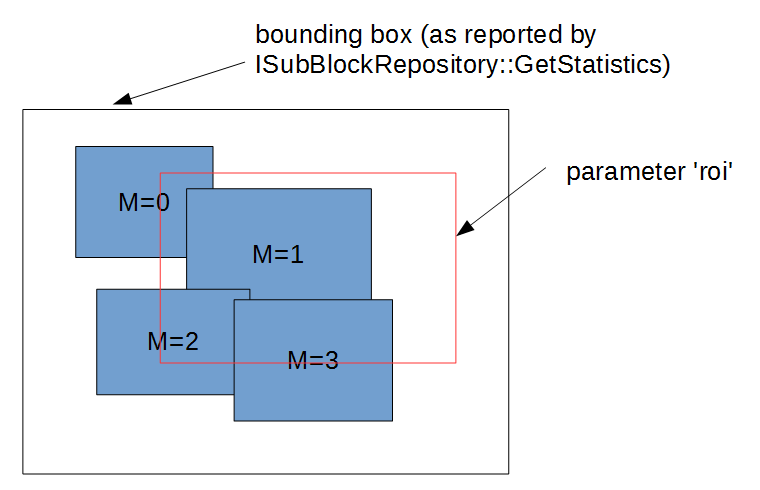
\includegraphics[width=\textwidth,height=\textheight/2,keepaspectratio=true]{SingleChannelTileAccessor_1.PNG}}
\end{DoxyImageNoCaption}
 The resulting output bitmap will look like this\+:  
\begin{DoxyImageNoCaption}
  \mbox{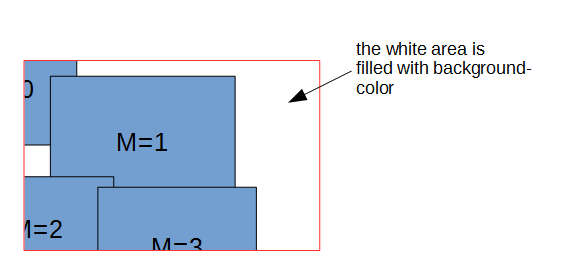
\includegraphics[width=\textwidth,height=\textheight/2,keepaspectratio=true]{SingleChannelTileAccessor_2.PNG}}
\end{DoxyImageNoCaption}
 This accessor only operates on pyramid layer 0 -\/ i. e. only sub-\/blocks with logical\+\_\+size = physical\+\_\+size will be considered. If the flag \char`\"{}draw\+Tile\+Border\char`\"{} is set, then the tiles will be sorted by their M-\/index (tiles with higher M-\/index are placed \textquotesingle{}on top\textquotesingle{}).~\newline
The pixel type of the output bitmap is either specified as an argument or it is automatically determined. In the latter case the first sub-\/block found on the specified plane is examined for its pixeltype, and this pixeltype is used.~\newline
The pixels in the output bitmap get converted from the source pixels (if their pixeltypes differs). 

\subsection{Member Function Documentation}
\mbox{\Hypertarget{classlib_c_z_i_1_1_i_single_channel_tile_accessor_a50e17c0c197bf5f782a67e044dd4e943}\label{classlib_c_z_i_1_1_i_single_channel_tile_accessor_a50e17c0c197bf5f782a67e044dd4e943}} 
\index{lib\+C\+Z\+I\+::\+I\+Single\+Channel\+Tile\+Accessor@{lib\+C\+Z\+I\+::\+I\+Single\+Channel\+Tile\+Accessor}!Get@{Get}}
\index{Get@{Get}!lib\+C\+Z\+I\+::\+I\+Single\+Channel\+Tile\+Accessor@{lib\+C\+Z\+I\+::\+I\+Single\+Channel\+Tile\+Accessor}}
\subsubsection{\texorpdfstring{Get()}{Get()}\hspace{0.1cm}{\footnotesize\ttfamily [1/5]}}
{\footnotesize\ttfamily virtual std\+::shared\+\_\+ptr$<$\hyperlink{classlib_c_z_i_1_1_i_bitmap_data}{lib\+C\+Z\+I\+::\+I\+Bitmap\+Data}$>$ lib\+C\+Z\+I\+::\+I\+Single\+Channel\+Tile\+Accessor\+::\+Get (\begin{DoxyParamCaption}\item[{const \hyperlink{structlib_c_z_i_1_1_int_rect}{lib\+C\+Z\+I\+::\+Int\+Rect} \&}]{roi,  }\item[{const \hyperlink{classlib_c_z_i_1_1_i_dim_coordinate}{I\+Dim\+Coordinate} $\ast$}]{plane\+Coordinate,  }\item[{const \hyperlink{structlib_c_z_i_1_1_i_single_channel_tile_accessor_1_1_options}{Options} $\ast$}]{p\+Options }\end{DoxyParamCaption})\hspace{0.3cm}{\ttfamily [pure virtual]}}



Gets the tile composite of the specified plane and the specified R\+OI. The pixeltype is determined by examing the first subblock found in the specified plane (which is an arbitrary subblock). A newly allocated bitmap is returned. 

It needs to be defined what is supposed to happen if there is no subblock found in the specified plane. 


\begin{DoxyParams}{Parameters}
{\em roi} & The R\+OI. \\
\hline
{\em plane\+Coordinate} & The plane coordinate. \\
\hline
{\em p\+Options} & \hyperlink{structlib_c_z_i_1_1_i_single_channel_tile_accessor_1_1_options}{Options} for controlling the operation. \\
\hline
\end{DoxyParams}
\begin{DoxyReturn}{Returns}
A std\+::shared\+\_\+ptr$<$\hyperlink{classlib_c_z_i_1_1_i_bitmap_data}{lib\+C\+Z\+I\+::\+I\+Bitmap\+Data}$>$ containing the tile-\/composite.
\end{DoxyReturn}
\mbox{\Hypertarget{classlib_c_z_i_1_1_i_single_channel_tile_accessor_a4fb81512693a2d7221abece14c33d1f3}\label{classlib_c_z_i_1_1_i_single_channel_tile_accessor_a4fb81512693a2d7221abece14c33d1f3}} 
\index{lib\+C\+Z\+I\+::\+I\+Single\+Channel\+Tile\+Accessor@{lib\+C\+Z\+I\+::\+I\+Single\+Channel\+Tile\+Accessor}!Get@{Get}}
\index{Get@{Get}!lib\+C\+Z\+I\+::\+I\+Single\+Channel\+Tile\+Accessor@{lib\+C\+Z\+I\+::\+I\+Single\+Channel\+Tile\+Accessor}}
\subsubsection{\texorpdfstring{Get()}{Get()}\hspace{0.1cm}{\footnotesize\ttfamily [2/5]}}
{\footnotesize\ttfamily virtual std\+::shared\+\_\+ptr$<$\hyperlink{classlib_c_z_i_1_1_i_bitmap_data}{lib\+C\+Z\+I\+::\+I\+Bitmap\+Data}$>$ lib\+C\+Z\+I\+::\+I\+Single\+Channel\+Tile\+Accessor\+::\+Get (\begin{DoxyParamCaption}\item[{\hyperlink{namespacelib_c_z_i_abf8ce12ab88b06c8b3b47efbb5e2e834}{lib\+C\+Z\+I\+::\+Pixel\+Type}}]{pixeltype,  }\item[{const \hyperlink{structlib_c_z_i_1_1_int_rect}{lib\+C\+Z\+I\+::\+Int\+Rect} \&}]{roi,  }\item[{const \hyperlink{classlib_c_z_i_1_1_i_dim_coordinate}{I\+Dim\+Coordinate} $\ast$}]{plane\+Coordinate,  }\item[{const \hyperlink{structlib_c_z_i_1_1_i_single_channel_tile_accessor_1_1_options}{Options} $\ast$}]{p\+Options }\end{DoxyParamCaption})\hspace{0.3cm}{\ttfamily [pure virtual]}}

Gets the tile composite of the specified plane and the specified R\+OI.


\begin{DoxyParams}{Parameters}
{\em pixeltype} & The pixeltype. \\
\hline
{\em roi} & The R\+OI. \\
\hline
{\em plane\+Coordinate} & The plane coordinate. \\
\hline
{\em p\+Options} & \hyperlink{structlib_c_z_i_1_1_i_single_channel_tile_accessor_1_1_options}{Options} for controlling the operation.\\
\hline
\end{DoxyParams}
\begin{DoxyReturn}{Returns}
A std\+::shared\+\_\+ptr$<$\hyperlink{classlib_c_z_i_1_1_i_bitmap_data}{lib\+C\+Z\+I\+::\+I\+Bitmap\+Data}$>$ containing the tile-\/composite. 
\end{DoxyReturn}
\mbox{\Hypertarget{classlib_c_z_i_1_1_i_single_channel_tile_accessor_a275295786554ca6dbf9f2d0b3086dcad}\label{classlib_c_z_i_1_1_i_single_channel_tile_accessor_a275295786554ca6dbf9f2d0b3086dcad}} 
\index{lib\+C\+Z\+I\+::\+I\+Single\+Channel\+Tile\+Accessor@{lib\+C\+Z\+I\+::\+I\+Single\+Channel\+Tile\+Accessor}!Get@{Get}}
\index{Get@{Get}!lib\+C\+Z\+I\+::\+I\+Single\+Channel\+Tile\+Accessor@{lib\+C\+Z\+I\+::\+I\+Single\+Channel\+Tile\+Accessor}}
\subsubsection{\texorpdfstring{Get()}{Get()}\hspace{0.1cm}{\footnotesize\ttfamily [3/5]}}
{\footnotesize\ttfamily virtual void lib\+C\+Z\+I\+::\+I\+Single\+Channel\+Tile\+Accessor\+::\+Get (\begin{DoxyParamCaption}\item[{\hyperlink{classlib_c_z_i_1_1_i_bitmap_data}{lib\+C\+Z\+I\+::\+I\+Bitmap\+Data} $\ast$}]{p\+Dest,  }\item[{int}]{x\+Pos,  }\item[{int}]{y\+Pos,  }\item[{const \hyperlink{classlib_c_z_i_1_1_i_dim_coordinate}{I\+Dim\+Coordinate} $\ast$}]{plane\+Coordinate,  }\item[{const \hyperlink{structlib_c_z_i_1_1_i_single_channel_tile_accessor_1_1_options}{Options} $\ast$}]{p\+Options }\end{DoxyParamCaption})\hspace{0.3cm}{\ttfamily [pure virtual]}}

Copy the tile composite into the specified bitmap. The bitmap passed in here determines the width and the height of the R\+OI (and the pixeltype).


\begin{DoxyParams}[1]{Parameters}
\mbox{\tt in}  & {\em p\+Dest} & The destination bitmap. \\
\hline
 & {\em x\+Pos} & The x-\/position of the R\+OI (width and height are given by p\+Dest). \\
\hline
 & {\em y\+Pos} & The y-\/position of the R\+OI ((width and height are given by p\+Dest). \\
\hline
 & {\em plane\+Coordinate} & The plane coordinate. \\
\hline
 & {\em p\+Options} & \hyperlink{structlib_c_z_i_1_1_i_single_channel_tile_accessor_1_1_options}{Options} for controlling the operation. \\
\hline
\end{DoxyParams}
\mbox{\Hypertarget{classlib_c_z_i_1_1_i_single_channel_tile_accessor_a9ef98a25e06e5da36d811705bb076dcc}\label{classlib_c_z_i_1_1_i_single_channel_tile_accessor_a9ef98a25e06e5da36d811705bb076dcc}} 
\index{lib\+C\+Z\+I\+::\+I\+Single\+Channel\+Tile\+Accessor@{lib\+C\+Z\+I\+::\+I\+Single\+Channel\+Tile\+Accessor}!Get@{Get}}
\index{Get@{Get}!lib\+C\+Z\+I\+::\+I\+Single\+Channel\+Tile\+Accessor@{lib\+C\+Z\+I\+::\+I\+Single\+Channel\+Tile\+Accessor}}
\subsubsection{\texorpdfstring{Get()}{Get()}\hspace{0.1cm}{\footnotesize\ttfamily [4/5]}}
{\footnotesize\ttfamily std\+::shared\+\_\+ptr$<$\hyperlink{classlib_c_z_i_1_1_i_bitmap_data}{lib\+C\+Z\+I\+::\+I\+Bitmap\+Data}$>$ lib\+C\+Z\+I\+::\+I\+Single\+Channel\+Tile\+Accessor\+::\+Get (\begin{DoxyParamCaption}\item[{int}]{x\+Pos,  }\item[{int}]{y\+Pos,  }\item[{int}]{width,  }\item[{int}]{height,  }\item[{const \hyperlink{classlib_c_z_i_1_1_i_dim_coordinate}{I\+Dim\+Coordinate} $\ast$}]{plane\+Coordinate,  }\item[{const \hyperlink{structlib_c_z_i_1_1_i_single_channel_tile_accessor_1_1_options}{Options} $\ast$}]{p\+Options }\end{DoxyParamCaption})\hspace{0.3cm}{\ttfamily [inline]}}

Gets the tile composite of the specified plane and the specified R\+OI. The pixeltype is determined by examing the first subblock found in the specified plane (which is an arbitrary subblock). A newly allocated bitmap is returned. 
\begin{DoxyParams}{Parameters}
{\em x\+Pos} & The x-\/position. \\
\hline
{\em y\+Pos} & The y-\/position. \\
\hline
{\em width} & The width. \\
\hline
{\em height} & The height. \\
\hline
{\em plane\+Coordinate} & The plane coordinate. \\
\hline
{\em p\+Options} & \hyperlink{structlib_c_z_i_1_1_i_single_channel_tile_accessor_1_1_options}{Options} for controlling the operation. \\
\hline
\end{DoxyParams}
\begin{DoxyReturn}{Returns}
A std\+::shared\+\_\+ptr$<$\hyperlink{classlib_c_z_i_1_1_i_bitmap_data}{lib\+C\+Z\+I\+::\+I\+Bitmap\+Data}$>$ 
\end{DoxyReturn}
\mbox{\Hypertarget{classlib_c_z_i_1_1_i_single_channel_tile_accessor_a8a9654ed1df4929068477a43597bf084}\label{classlib_c_z_i_1_1_i_single_channel_tile_accessor_a8a9654ed1df4929068477a43597bf084}} 
\index{lib\+C\+Z\+I\+::\+I\+Single\+Channel\+Tile\+Accessor@{lib\+C\+Z\+I\+::\+I\+Single\+Channel\+Tile\+Accessor}!Get@{Get}}
\index{Get@{Get}!lib\+C\+Z\+I\+::\+I\+Single\+Channel\+Tile\+Accessor@{lib\+C\+Z\+I\+::\+I\+Single\+Channel\+Tile\+Accessor}}
\subsubsection{\texorpdfstring{Get()}{Get()}\hspace{0.1cm}{\footnotesize\ttfamily [5/5]}}
{\footnotesize\ttfamily std\+::shared\+\_\+ptr$<$\hyperlink{classlib_c_z_i_1_1_i_bitmap_data}{lib\+C\+Z\+I\+::\+I\+Bitmap\+Data}$>$ lib\+C\+Z\+I\+::\+I\+Single\+Channel\+Tile\+Accessor\+::\+Get (\begin{DoxyParamCaption}\item[{\hyperlink{namespacelib_c_z_i_abf8ce12ab88b06c8b3b47efbb5e2e834}{lib\+C\+Z\+I\+::\+Pixel\+Type}}]{pixeltype,  }\item[{int}]{x\+Pos,  }\item[{int}]{y\+Pos,  }\item[{int}]{width,  }\item[{int}]{height,  }\item[{const \hyperlink{classlib_c_z_i_1_1_i_dim_coordinate}{I\+Dim\+Coordinate} $\ast$}]{plane\+Coordinate,  }\item[{const \hyperlink{structlib_c_z_i_1_1_i_single_channel_tile_accessor_1_1_options}{Options} $\ast$}]{p\+Options }\end{DoxyParamCaption})\hspace{0.3cm}{\ttfamily [inline]}}

Gets the tile composite of the specified plane and the specified R\+OI. 
\begin{DoxyParams}{Parameters}
{\em pixeltype} & The pixeltype. \\
\hline
{\em x\+Pos} & The x-\/position. \\
\hline
{\em y\+Pos} & The y-\/position. \\
\hline
{\em width} & The width. \\
\hline
{\em height} & The height. \\
\hline
{\em plane\+Coordinate} & The plane coordinate. \\
\hline
{\em p\+Options} & \hyperlink{structlib_c_z_i_1_1_i_single_channel_tile_accessor_1_1_options}{Options} for controlling the operation. \\
\hline
\end{DoxyParams}
\begin{DoxyReturn}{Returns}
A std\+::shared\+\_\+ptr$<$\hyperlink{classlib_c_z_i_1_1_i_bitmap_data}{lib\+C\+Z\+I\+::\+I\+Bitmap\+Data}$>$ 
\end{DoxyReturn}


The documentation for this class was generated from the following file\+:\begin{DoxyCompactItemize}
\item 
lib\+C\+Z\+I/lib\+C\+Z\+I\+\_\+\+Compositor.\+h\end{DoxyCompactItemize}

\hypertarget{classlib_c_z_i_1_1_i_site}{}\section{lib\+C\+ZI\+:\+:I\+Site Class Reference}
\label{classlib_c_z_i_1_1_i_site}\index{lib\+C\+Z\+I\+::\+I\+Site@{lib\+C\+Z\+I\+::\+I\+Site}}


{\ttfamily \#include $<$lib\+C\+Z\+I\+\_\+\+Site.\+h$>$}

\subsection*{Public Member Functions}
\begin{DoxyCompactItemize}
\item 
virtual bool \hyperlink{classlib_c_z_i_1_1_i_site_a56c0d12cfa78ecb83fb5bbd0f500ee30}{Is\+Enabled} (int log\+Level)=0
\item 
virtual void \hyperlink{classlib_c_z_i_1_1_i_site_aa709ab923626e1a17898b3d6802c2082}{Log} (int level, const char $\ast$sz\+Msg)=0
\item 
virtual std\+::shared\+\_\+ptr$<$ \hyperlink{classlib_c_z_i_1_1_i_decoder}{I\+Decoder} $>$ \hyperlink{classlib_c_z_i_1_1_i_site_a2cbf7eccd867378b4943519284b98ef1}{Get\+Decoder} (\hyperlink{namespacelib_c_z_i_a68cd7521fd89880f820ea55baf6f6179}{Image\+Decoder\+Type} type, const char $\ast$arguments)=0
\item 
virtual std\+::shared\+\_\+ptr$<$ \hyperlink{classlib_c_z_i_1_1_i_bitmap_data}{lib\+C\+Z\+I\+::\+I\+Bitmap\+Data} $>$ \hyperlink{classlib_c_z_i_1_1_i_site_ab1b59f522c0dfdce2474036e4ac6cc23}{Create\+Bitmap} (\hyperlink{namespacelib_c_z_i_abf8ce12ab88b06c8b3b47efbb5e2e834}{lib\+C\+Z\+I\+::\+Pixel\+Type} pixeltype, std\+::uint32\+\_\+t width, std\+::uint32\+\_\+t height, std\+::uint32\+\_\+t stride=0, std\+::uint32\+\_\+t extra\+Rows=0, std\+::uint32\+\_\+t extra\+Columns=0)=0
\item 
void \hyperlink{classlib_c_z_i_1_1_i_site_af879b88237db67ebf48f9c48fc15f57f}{Log} (int level, const std\+::string \&str)
\item 
void \hyperlink{classlib_c_z_i_1_1_i_site_a3485af37a7034750ee9d90efa9fcf2c7}{Log} (int level, std\+::stringstream \&ss)
\end{DoxyCompactItemize}


\subsection{Detailed Description}
Interface for the Site-\/object. It is intented for customizing the library (by injecting a custom implementation of this interface). 

\subsection{Member Function Documentation}
\mbox{\Hypertarget{classlib_c_z_i_1_1_i_site_ab1b59f522c0dfdce2474036e4ac6cc23}\label{classlib_c_z_i_1_1_i_site_ab1b59f522c0dfdce2474036e4ac6cc23}} 
\index{lib\+C\+Z\+I\+::\+I\+Site@{lib\+C\+Z\+I\+::\+I\+Site}!Create\+Bitmap@{Create\+Bitmap}}
\index{Create\+Bitmap@{Create\+Bitmap}!lib\+C\+Z\+I\+::\+I\+Site@{lib\+C\+Z\+I\+::\+I\+Site}}
\subsubsection{\texorpdfstring{Create\+Bitmap()}{CreateBitmap()}}
{\footnotesize\ttfamily virtual std\+::shared\+\_\+ptr$<$\hyperlink{classlib_c_z_i_1_1_i_bitmap_data}{lib\+C\+Z\+I\+::\+I\+Bitmap\+Data}$>$ lib\+C\+Z\+I\+::\+I\+Site\+::\+Create\+Bitmap (\begin{DoxyParamCaption}\item[{\hyperlink{namespacelib_c_z_i_abf8ce12ab88b06c8b3b47efbb5e2e834}{lib\+C\+Z\+I\+::\+Pixel\+Type}}]{pixeltype,  }\item[{std\+::uint32\+\_\+t}]{width,  }\item[{std\+::uint32\+\_\+t}]{height,  }\item[{std\+::uint32\+\_\+t}]{stride = {\ttfamily 0},  }\item[{std\+::uint32\+\_\+t}]{extra\+Rows = {\ttfamily 0},  }\item[{std\+::uint32\+\_\+t}]{extra\+Columns = {\ttfamily 0} }\end{DoxyParamCaption})\hspace{0.3cm}{\ttfamily [pure virtual]}}

Creates a bitmap object. All internal bitmap allocations are done with this method, and overloading this method allows to use a externally controlled memory management to be injected.


\begin{DoxyParams}{Parameters}
{\em pixeltype} & The pixeltype of the newly allocated bitmap. \\
\hline
{\em width} & The width of the newly allocated bitmap. \\
\hline
{\em height} & The height of the newly allocated bitmap. \\
\hline
{\em stride} & The stride of the newly allocated bitmap. If $<$= 0, then the method may choose an appropriate stride on its own. If a stride $>$0 is given here, then we expect that the newly created bitmap adheres to it. \\
\hline
{\em extra\+Rows} & The extra rows (not currently used, will always be 0). \\
\hline
{\em extra\+Columns} & The extra columns (not currently used, will always be 0).\\
\hline
\end{DoxyParams}
\begin{DoxyReturn}{Returns}
The newly allocated bitmap. 
\end{DoxyReturn}
\mbox{\Hypertarget{classlib_c_z_i_1_1_i_site_a2cbf7eccd867378b4943519284b98ef1}\label{classlib_c_z_i_1_1_i_site_a2cbf7eccd867378b4943519284b98ef1}} 
\index{lib\+C\+Z\+I\+::\+I\+Site@{lib\+C\+Z\+I\+::\+I\+Site}!Get\+Decoder@{Get\+Decoder}}
\index{Get\+Decoder@{Get\+Decoder}!lib\+C\+Z\+I\+::\+I\+Site@{lib\+C\+Z\+I\+::\+I\+Site}}
\subsubsection{\texorpdfstring{Get\+Decoder()}{GetDecoder()}}
{\footnotesize\ttfamily virtual std\+::shared\+\_\+ptr$<$\hyperlink{classlib_c_z_i_1_1_i_decoder}{I\+Decoder}$>$ lib\+C\+Z\+I\+::\+I\+Site\+::\+Get\+Decoder (\begin{DoxyParamCaption}\item[{\hyperlink{namespacelib_c_z_i_a68cd7521fd89880f820ea55baf6f6179}{Image\+Decoder\+Type}}]{type,  }\item[{const char $\ast$}]{arguments }\end{DoxyParamCaption})\hspace{0.3cm}{\ttfamily [pure virtual]}}

Gets a decoder object.


\begin{DoxyParams}{Parameters}
{\em type} & The type. \\
\hline
{\em arguments} & The arguments.\\
\hline
\end{DoxyParams}
\begin{DoxyReturn}{Returns}
The decoder object. 
\end{DoxyReturn}
\mbox{\Hypertarget{classlib_c_z_i_1_1_i_site_a56c0d12cfa78ecb83fb5bbd0f500ee30}\label{classlib_c_z_i_1_1_i_site_a56c0d12cfa78ecb83fb5bbd0f500ee30}} 
\index{lib\+C\+Z\+I\+::\+I\+Site@{lib\+C\+Z\+I\+::\+I\+Site}!Is\+Enabled@{Is\+Enabled}}
\index{Is\+Enabled@{Is\+Enabled}!lib\+C\+Z\+I\+::\+I\+Site@{lib\+C\+Z\+I\+::\+I\+Site}}
\subsubsection{\texorpdfstring{Is\+Enabled()}{IsEnabled()}}
{\footnotesize\ttfamily virtual bool lib\+C\+Z\+I\+::\+I\+Site\+::\+Is\+Enabled (\begin{DoxyParamCaption}\item[{int}]{log\+Level }\end{DoxyParamCaption})\hspace{0.3cm}{\ttfamily [pure virtual]}}

Query if the specified logging level is enabled. In the case that constructing the message to be logged takes a significant amount of resources (i. e. time or memory), this method should be called before in order to determine whether the output is required at all. This also means that this method may be called very frequently, so implementors should take care that it executes reasonably fast.


\begin{DoxyParams}{Parameters}
{\em log\+Level} & The logging level.\\
\hline
\end{DoxyParams}
\begin{DoxyReturn}{Returns}
True if the specified logging level is enabled, false otherwise. 
\end{DoxyReturn}
\mbox{\Hypertarget{classlib_c_z_i_1_1_i_site_aa709ab923626e1a17898b3d6802c2082}\label{classlib_c_z_i_1_1_i_site_aa709ab923626e1a17898b3d6802c2082}} 
\index{lib\+C\+Z\+I\+::\+I\+Site@{lib\+C\+Z\+I\+::\+I\+Site}!Log@{Log}}
\index{Log@{Log}!lib\+C\+Z\+I\+::\+I\+Site@{lib\+C\+Z\+I\+::\+I\+Site}}
\subsubsection{\texorpdfstring{Log()}{Log()}\hspace{0.1cm}{\footnotesize\ttfamily [1/3]}}
{\footnotesize\ttfamily virtual void lib\+C\+Z\+I\+::\+I\+Site\+::\+Log (\begin{DoxyParamCaption}\item[{int}]{level,  }\item[{const char $\ast$}]{sz\+Msg }\end{DoxyParamCaption})\hspace{0.3cm}{\ttfamily [pure virtual]}}

Output the specified string at the specified logging level. \begin{DoxyRemark}{Remarks}
The text is assumed to be A\+S\+C\+II -\/ not U\+T\+F8 or any other codepage. Use only plain-\/\+A\+S\+C\+II. This might change... 
\end{DoxyRemark}

\begin{DoxyParams}{Parameters}
{\em level} & The logging level. \\
\hline
{\em sz\+Msg} & The message to be logged. \\
\hline
\end{DoxyParams}
\mbox{\Hypertarget{classlib_c_z_i_1_1_i_site_af879b88237db67ebf48f9c48fc15f57f}\label{classlib_c_z_i_1_1_i_site_af879b88237db67ebf48f9c48fc15f57f}} 
\index{lib\+C\+Z\+I\+::\+I\+Site@{lib\+C\+Z\+I\+::\+I\+Site}!Log@{Log}}
\index{Log@{Log}!lib\+C\+Z\+I\+::\+I\+Site@{lib\+C\+Z\+I\+::\+I\+Site}}
\subsubsection{\texorpdfstring{Log()}{Log()}\hspace{0.1cm}{\footnotesize\ttfamily [2/3]}}
{\footnotesize\ttfamily void lib\+C\+Z\+I\+::\+I\+Site\+::\+Log (\begin{DoxyParamCaption}\item[{int}]{level,  }\item[{const std\+::string \&}]{str }\end{DoxyParamCaption})\hspace{0.3cm}{\ttfamily [inline]}}

Output the specified string at the specified logging level. 
\begin{DoxyParams}{Parameters}
{\em level} & The level. \\
\hline
{\em str} & The string. \\
\hline
\end{DoxyParams}
\mbox{\Hypertarget{classlib_c_z_i_1_1_i_site_a3485af37a7034750ee9d90efa9fcf2c7}\label{classlib_c_z_i_1_1_i_site_a3485af37a7034750ee9d90efa9fcf2c7}} 
\index{lib\+C\+Z\+I\+::\+I\+Site@{lib\+C\+Z\+I\+::\+I\+Site}!Log@{Log}}
\index{Log@{Log}!lib\+C\+Z\+I\+::\+I\+Site@{lib\+C\+Z\+I\+::\+I\+Site}}
\subsubsection{\texorpdfstring{Log()}{Log()}\hspace{0.1cm}{\footnotesize\ttfamily [3/3]}}
{\footnotesize\ttfamily void lib\+C\+Z\+I\+::\+I\+Site\+::\+Log (\begin{DoxyParamCaption}\item[{int}]{level,  }\item[{std\+::stringstream \&}]{ss }\end{DoxyParamCaption})\hspace{0.3cm}{\ttfamily [inline]}}

Output the specified stringstream object at the specified logging level. 
\begin{DoxyParams}[1]{Parameters}
 & {\em level} & The level. \\
\hline
\mbox{\tt in}  & {\em ss} & The stringstream object. \\
\hline
\end{DoxyParams}


The documentation for this class was generated from the following file\+:\begin{DoxyCompactItemize}
\item 
lib\+C\+Z\+I/lib\+C\+Z\+I\+\_\+\+Site.\+h\end{DoxyCompactItemize}

\hypertarget{classlib_c_z_i_1_1_i_stream}{}\section{lib\+C\+ZI\+:\+:I\+Stream Class Reference}
\label{classlib_c_z_i_1_1_i_stream}\index{lib\+C\+Z\+I\+::\+I\+Stream@{lib\+C\+Z\+I\+::\+I\+Stream}}


{\ttfamily \#include $<$lib\+C\+Z\+I.\+h$>$}

\subsection*{Public Member Functions}
\begin{DoxyCompactItemize}
\item 
virtual void \hyperlink{classlib_c_z_i_1_1_i_stream_ae275276d0da5082a3711527ddfedfd9f}{Read} (std\+::uint64\+\_\+t offset, void $\ast$pv, std\+::uint64\+\_\+t size, std\+::uint64\+\_\+t $\ast$ptr\+Bytes\+Read)=0
\end{DoxyCompactItemize}


\subsection{Detailed Description}
Interface used for accessing the data-\/stream. 

\subsection{Member Function Documentation}
\mbox{\Hypertarget{classlib_c_z_i_1_1_i_stream_ae275276d0da5082a3711527ddfedfd9f}\label{classlib_c_z_i_1_1_i_stream_ae275276d0da5082a3711527ddfedfd9f}} 
\index{lib\+C\+Z\+I\+::\+I\+Stream@{lib\+C\+Z\+I\+::\+I\+Stream}!Read@{Read}}
\index{Read@{Read}!lib\+C\+Z\+I\+::\+I\+Stream@{lib\+C\+Z\+I\+::\+I\+Stream}}
\subsubsection{\texorpdfstring{Read()}{Read()}}
{\footnotesize\ttfamily virtual void lib\+C\+Z\+I\+::\+I\+Stream\+::\+Read (\begin{DoxyParamCaption}\item[{std\+::uint64\+\_\+t}]{offset,  }\item[{void $\ast$}]{pv,  }\item[{std\+::uint64\+\_\+t}]{size,  }\item[{std\+::uint64\+\_\+t $\ast$}]{ptr\+Bytes\+Read }\end{DoxyParamCaption})\hspace{0.3cm}{\ttfamily [pure virtual]}}

Reads the specified amount of data from the stream at the specified position.


\begin{DoxyParams}[1]{Parameters}
 & {\em offset} & The offset to start reading from. \\
\hline
\mbox{\tt out}  & {\em pv} & The caller-\/provided buffer for the data. Must be non-\/null. \\
\hline
 & {\em size} & The size of the buffer. \\
\hline
\mbox{\tt out}  & {\em ptr\+Bytes\+Read} & If non-\/null, the variable pointed to will receive the number of bytes actually read. \\
\hline
\end{DoxyParams}


The documentation for this class was generated from the following file\+:\begin{DoxyCompactItemize}
\item 
lib\+C\+Z\+I/lib\+C\+Z\+I.\+h\end{DoxyCompactItemize}

\hypertarget{classlib_c_z_i_1_1_i_sub_block}{}\section{lib\+C\+ZI\+:\+:I\+Sub\+Block Class Reference}
\label{classlib_c_z_i_1_1_i_sub_block}\index{lib\+C\+Z\+I\+::\+I\+Sub\+Block@{lib\+C\+Z\+I\+::\+I\+Sub\+Block}}


{\ttfamily \#include $<$lib\+C\+Z\+I.\+h$>$}

\subsection*{Public Types}
\begin{DoxyCompactItemize}
\item 
enum \hyperlink{classlib_c_z_i_1_1_i_sub_block_a4dc4926ea65d8d20310b8b79ea76e108}{Mem\+Blk\+Type} \{ \hyperlink{classlib_c_z_i_1_1_i_sub_block_a4dc4926ea65d8d20310b8b79ea76e108ada66dacad65a36fd265a7a2dacae197c}{Metadata}, 
\hyperlink{classlib_c_z_i_1_1_i_sub_block_a4dc4926ea65d8d20310b8b79ea76e108ad89f4242d3c09c1ef3302841226d240d}{Data}, 
\hyperlink{classlib_c_z_i_1_1_i_sub_block_a4dc4926ea65d8d20310b8b79ea76e108ab60de398d6a7a2fe1c4c9585572b3ef1}{Attachment}
 \}\begin{DoxyCompactList}\small\item\em Values that represent the three different data types found in a sub-\/block. \end{DoxyCompactList}
\end{DoxyCompactItemize}
\subsection*{Public Member Functions}
\begin{DoxyCompactItemize}
\item 
virtual const \hyperlink{structlib_c_z_i_1_1_sub_block_info}{Sub\+Block\+Info} \& \hyperlink{classlib_c_z_i_1_1_i_sub_block_a557108549db08e25b1df1ef8fae37a07}{Get\+Sub\+Block\+Info} () const =0
\item 
virtual void \hyperlink{classlib_c_z_i_1_1_i_sub_block_a6f84a58437af59bac64a6147369ddae4}{Dangerous\+Get\+Raw\+Data} (\hyperlink{classlib_c_z_i_1_1_i_sub_block_a4dc4926ea65d8d20310b8b79ea76e108}{Mem\+Blk\+Type} type, const void $\ast$\&ptr, size\+\_\+t \&size) const =0
\item 
virtual std\+::shared\+\_\+ptr$<$ const void $>$ \hyperlink{classlib_c_z_i_1_1_i_sub_block_a55ec2c117050df253367661f9cd606cf}{Get\+Raw\+Data} (\hyperlink{classlib_c_z_i_1_1_i_sub_block_a4dc4926ea65d8d20310b8b79ea76e108}{Mem\+Blk\+Type} type, size\+\_\+t $\ast$ptr\+Size)=0
\item 
virtual std\+::shared\+\_\+ptr$<$ \hyperlink{classlib_c_z_i_1_1_i_bitmap_data}{I\+Bitmap\+Data} $>$ \hyperlink{classlib_c_z_i_1_1_i_sub_block_af2059d1f270f3e4349244403fa7dd71c}{Create\+Bitmap} ()=0
\item 
{\footnotesize template$<$class Q $>$ }\\void \hyperlink{classlib_c_z_i_1_1_i_sub_block_acd9396cc5d366de99b37a26c98031d66}{Dangerous\+Get\+Raw\+Data} (\hyperlink{classlib_c_z_i_1_1_i_sub_block_a4dc4926ea65d8d20310b8b79ea76e108}{Mem\+Blk\+Type} type, const Q $\ast$\&ptr, size\+\_\+t \&size) const
\end{DoxyCompactItemize}


\subsection{Detailed Description}
Representation of a sub-\/block. A sub-\/block can contain three types of data\+: the bitmap-\/data, an attachment and metadata. The presence of an attachment is optional. 

\subsection{Member Enumeration Documentation}
\mbox{\Hypertarget{classlib_c_z_i_1_1_i_sub_block_a4dc4926ea65d8d20310b8b79ea76e108}\label{classlib_c_z_i_1_1_i_sub_block_a4dc4926ea65d8d20310b8b79ea76e108}} 
\index{lib\+C\+Z\+I\+::\+I\+Sub\+Block@{lib\+C\+Z\+I\+::\+I\+Sub\+Block}!Mem\+Blk\+Type@{Mem\+Blk\+Type}}
\index{Mem\+Blk\+Type@{Mem\+Blk\+Type}!lib\+C\+Z\+I\+::\+I\+Sub\+Block@{lib\+C\+Z\+I\+::\+I\+Sub\+Block}}
\subsubsection{\texorpdfstring{Mem\+Blk\+Type}{MemBlkType}}
{\footnotesize\ttfamily enum \hyperlink{classlib_c_z_i_1_1_i_sub_block_a4dc4926ea65d8d20310b8b79ea76e108}{lib\+C\+Z\+I\+::\+I\+Sub\+Block\+::\+Mem\+Blk\+Type}}



Values that represent the three different data types found in a sub-\/block. 

\begin{DoxyEnumFields}{Enumerator}
\raisebox{\heightof{T}}[0pt][0pt]{\index{Metadata@{Metadata}!lib\+C\+Z\+I\+::\+I\+Sub\+Block@{lib\+C\+Z\+I\+::\+I\+Sub\+Block}}\index{lib\+C\+Z\+I\+::\+I\+Sub\+Block@{lib\+C\+Z\+I\+::\+I\+Sub\+Block}!Metadata@{Metadata}}}\mbox{\Hypertarget{classlib_c_z_i_1_1_i_sub_block_a4dc4926ea65d8d20310b8b79ea76e108ada66dacad65a36fd265a7a2dacae197c}\label{classlib_c_z_i_1_1_i_sub_block_a4dc4926ea65d8d20310b8b79ea76e108ada66dacad65a36fd265a7a2dacae197c}} 
Metadata&An enum constant representing the metadata. \\
\hline

\raisebox{\heightof{T}}[0pt][0pt]{\index{Data@{Data}!lib\+C\+Z\+I\+::\+I\+Sub\+Block@{lib\+C\+Z\+I\+::\+I\+Sub\+Block}}\index{lib\+C\+Z\+I\+::\+I\+Sub\+Block@{lib\+C\+Z\+I\+::\+I\+Sub\+Block}!Data@{Data}}}\mbox{\Hypertarget{classlib_c_z_i_1_1_i_sub_block_a4dc4926ea65d8d20310b8b79ea76e108ad89f4242d3c09c1ef3302841226d240d}\label{classlib_c_z_i_1_1_i_sub_block_a4dc4926ea65d8d20310b8b79ea76e108ad89f4242d3c09c1ef3302841226d240d}} 
Data&An enum constant representing the bitmap-\/data. \\
\hline

\raisebox{\heightof{T}}[0pt][0pt]{\index{Attachment@{Attachment}!lib\+C\+Z\+I\+::\+I\+Sub\+Block@{lib\+C\+Z\+I\+::\+I\+Sub\+Block}}\index{lib\+C\+Z\+I\+::\+I\+Sub\+Block@{lib\+C\+Z\+I\+::\+I\+Sub\+Block}!Attachment@{Attachment}}}\mbox{\Hypertarget{classlib_c_z_i_1_1_i_sub_block_a4dc4926ea65d8d20310b8b79ea76e108ab60de398d6a7a2fe1c4c9585572b3ef1}\label{classlib_c_z_i_1_1_i_sub_block_a4dc4926ea65d8d20310b8b79ea76e108ab60de398d6a7a2fe1c4c9585572b3ef1}} 
Attachment&An enum constant representing the attachment (of a sub-\/block). \\
\hline

\end{DoxyEnumFields}


\subsection{Member Function Documentation}
\mbox{\Hypertarget{classlib_c_z_i_1_1_i_sub_block_af2059d1f270f3e4349244403fa7dd71c}\label{classlib_c_z_i_1_1_i_sub_block_af2059d1f270f3e4349244403fa7dd71c}} 
\index{lib\+C\+Z\+I\+::\+I\+Sub\+Block@{lib\+C\+Z\+I\+::\+I\+Sub\+Block}!Create\+Bitmap@{Create\+Bitmap}}
\index{Create\+Bitmap@{Create\+Bitmap}!lib\+C\+Z\+I\+::\+I\+Sub\+Block@{lib\+C\+Z\+I\+::\+I\+Sub\+Block}}
\subsubsection{\texorpdfstring{Create\+Bitmap()}{CreateBitmap()}}
{\footnotesize\ttfamily virtual std\+::shared\+\_\+ptr$<$\hyperlink{classlib_c_z_i_1_1_i_bitmap_data}{I\+Bitmap\+Data}$>$ lib\+C\+Z\+I\+::\+I\+Sub\+Block\+::\+Create\+Bitmap (\begin{DoxyParamCaption}{ }\end{DoxyParamCaption})\hspace{0.3cm}{\ttfamily [pure virtual]}}

Creates a bitmap (from the data of this sub-\/block). \begin{DoxyRemark}{Remarks}
Within this call the bitmap is decoded (if necessary). In current implementation, the sub-\/block does not hold a reference to the returned bitmap here (and, if called twice, a new bitmap is created). One should not rely on this behavior, it is conceivable that in a later version the sub-\/block will keep a reference (and return the same bitmap if called twice). In current version this method is equivalent to calling Create\+Bitmap\+From\+Sub\+Block. 
\end{DoxyRemark}
\begin{DoxyReturn}{Returns}
The bitmap (contained in this sub-\/block). 
\end{DoxyReturn}
\mbox{\Hypertarget{classlib_c_z_i_1_1_i_sub_block_a6f84a58437af59bac64a6147369ddae4}\label{classlib_c_z_i_1_1_i_sub_block_a6f84a58437af59bac64a6147369ddae4}} 
\index{lib\+C\+Z\+I\+::\+I\+Sub\+Block@{lib\+C\+Z\+I\+::\+I\+Sub\+Block}!Dangerous\+Get\+Raw\+Data@{Dangerous\+Get\+Raw\+Data}}
\index{Dangerous\+Get\+Raw\+Data@{Dangerous\+Get\+Raw\+Data}!lib\+C\+Z\+I\+::\+I\+Sub\+Block@{lib\+C\+Z\+I\+::\+I\+Sub\+Block}}
\subsubsection{\texorpdfstring{Dangerous\+Get\+Raw\+Data()}{DangerousGetRawData()}\hspace{0.1cm}{\footnotesize\ttfamily [1/2]}}
{\footnotesize\ttfamily virtual void lib\+C\+Z\+I\+::\+I\+Sub\+Block\+::\+Dangerous\+Get\+Raw\+Data (\begin{DoxyParamCaption}\item[{\hyperlink{classlib_c_z_i_1_1_i_sub_block_a4dc4926ea65d8d20310b8b79ea76e108}{Mem\+Blk\+Type}}]{type,  }\item[{const void $\ast$\&}]{ptr,  }\item[{size\+\_\+t \&}]{size }\end{DoxyParamCaption}) const\hspace{0.3cm}{\ttfamily [pure virtual]}}

Get a pointer to the raw data. Note that the pointer returned is only valid during the lifetime of the sub-\/block-\/object. 
\begin{DoxyParams}[1]{Parameters}
 & {\em type} & The sub-\/block data-\/type. \\
\hline
\mbox{\tt out}  & {\em ptr} & The pointer to the data is stored here. \\
\hline
\mbox{\tt out}  & {\em size} & The size of the data. \\
\hline
\end{DoxyParams}
\mbox{\Hypertarget{classlib_c_z_i_1_1_i_sub_block_acd9396cc5d366de99b37a26c98031d66}\label{classlib_c_z_i_1_1_i_sub_block_acd9396cc5d366de99b37a26c98031d66}} 
\index{lib\+C\+Z\+I\+::\+I\+Sub\+Block@{lib\+C\+Z\+I\+::\+I\+Sub\+Block}!Dangerous\+Get\+Raw\+Data@{Dangerous\+Get\+Raw\+Data}}
\index{Dangerous\+Get\+Raw\+Data@{Dangerous\+Get\+Raw\+Data}!lib\+C\+Z\+I\+::\+I\+Sub\+Block@{lib\+C\+Z\+I\+::\+I\+Sub\+Block}}
\subsubsection{\texorpdfstring{Dangerous\+Get\+Raw\+Data()}{DangerousGetRawData()}\hspace{0.1cm}{\footnotesize\ttfamily [2/2]}}
{\footnotesize\ttfamily template$<$class Q $>$ \\
void lib\+C\+Z\+I\+::\+I\+Sub\+Block\+::\+Dangerous\+Get\+Raw\+Data (\begin{DoxyParamCaption}\item[{\hyperlink{classlib_c_z_i_1_1_i_sub_block_a4dc4926ea65d8d20310b8b79ea76e108}{Mem\+Blk\+Type}}]{type,  }\item[{const Q $\ast$\&}]{ptr,  }\item[{size\+\_\+t \&}]{size }\end{DoxyParamCaption}) const\hspace{0.3cm}{\ttfamily [inline]}}

A helper method used to cast the pointer to a specific type. 
\begin{DoxyParams}[1]{Parameters}
 & {\em type} & The sub-\/block data-\/type. \\
\hline
\mbox{\tt out}  & {\em ptr} & The pointer to the data is stored here. \\
\hline
\mbox{\tt out}  & {\em size} & The size of the data. \\
\hline
\end{DoxyParams}
\mbox{\Hypertarget{classlib_c_z_i_1_1_i_sub_block_a55ec2c117050df253367661f9cd606cf}\label{classlib_c_z_i_1_1_i_sub_block_a55ec2c117050df253367661f9cd606cf}} 
\index{lib\+C\+Z\+I\+::\+I\+Sub\+Block@{lib\+C\+Z\+I\+::\+I\+Sub\+Block}!Get\+Raw\+Data@{Get\+Raw\+Data}}
\index{Get\+Raw\+Data@{Get\+Raw\+Data}!lib\+C\+Z\+I\+::\+I\+Sub\+Block@{lib\+C\+Z\+I\+::\+I\+Sub\+Block}}
\subsubsection{\texorpdfstring{Get\+Raw\+Data()}{GetRawData()}}
{\footnotesize\ttfamily virtual std\+::shared\+\_\+ptr$<$const void$>$ lib\+C\+Z\+I\+::\+I\+Sub\+Block\+::\+Get\+Raw\+Data (\begin{DoxyParamCaption}\item[{\hyperlink{classlib_c_z_i_1_1_i_sub_block_a4dc4926ea65d8d20310b8b79ea76e108}{Mem\+Blk\+Type}}]{type,  }\item[{size\+\_\+t $\ast$}]{ptr\+Size }\end{DoxyParamCaption})\hspace{0.3cm}{\ttfamily [pure virtual]}}

Gets raw data. 
\begin{DoxyParams}[1]{Parameters}
 & {\em type} & The type. \\
\hline
\mbox{\tt out}  & {\em ptr\+Size} & If non-\/null, size of the data buffer is stored here. \\
\hline
\end{DoxyParams}
\begin{DoxyReturn}{Returns}
The raw data. 
\end{DoxyReturn}
\mbox{\Hypertarget{classlib_c_z_i_1_1_i_sub_block_a557108549db08e25b1df1ef8fae37a07}\label{classlib_c_z_i_1_1_i_sub_block_a557108549db08e25b1df1ef8fae37a07}} 
\index{lib\+C\+Z\+I\+::\+I\+Sub\+Block@{lib\+C\+Z\+I\+::\+I\+Sub\+Block}!Get\+Sub\+Block\+Info@{Get\+Sub\+Block\+Info}}
\index{Get\+Sub\+Block\+Info@{Get\+Sub\+Block\+Info}!lib\+C\+Z\+I\+::\+I\+Sub\+Block@{lib\+C\+Z\+I\+::\+I\+Sub\+Block}}
\subsubsection{\texorpdfstring{Get\+Sub\+Block\+Info()}{GetSubBlockInfo()}}
{\footnotesize\ttfamily virtual const \hyperlink{structlib_c_z_i_1_1_sub_block_info}{Sub\+Block\+Info}\& lib\+C\+Z\+I\+::\+I\+Sub\+Block\+::\+Get\+Sub\+Block\+Info (\begin{DoxyParamCaption}{ }\end{DoxyParamCaption}) const\hspace{0.3cm}{\ttfamily [pure virtual]}}

Gets sub-\/block information. \begin{DoxyReturn}{Returns}
The sub-\/block information. 
\end{DoxyReturn}


The documentation for this class was generated from the following file\+:\begin{DoxyCompactItemize}
\item 
lib\+C\+Z\+I/lib\+C\+Z\+I.\+h\end{DoxyCompactItemize}

\hypertarget{classlib_c_z_i_1_1_i_sub_block_repository}{}\section{lib\+C\+ZI\+:\+:I\+Sub\+Block\+Repository Class Reference}
\label{classlib_c_z_i_1_1_i_sub_block_repository}\index{lib\+C\+Z\+I\+::\+I\+Sub\+Block\+Repository@{lib\+C\+Z\+I\+::\+I\+Sub\+Block\+Repository}}


Interface for sub-\/block repository. This interface is used to access the sub-\/blocks in a C\+Z\+I-\/file.  




{\ttfamily \#include $<$lib\+C\+Z\+I.\+h$>$}

Inheritance diagram for lib\+C\+ZI\+:\+:I\+Sub\+Block\+Repository\+:\begin{figure}[H]
\begin{center}
\leavevmode
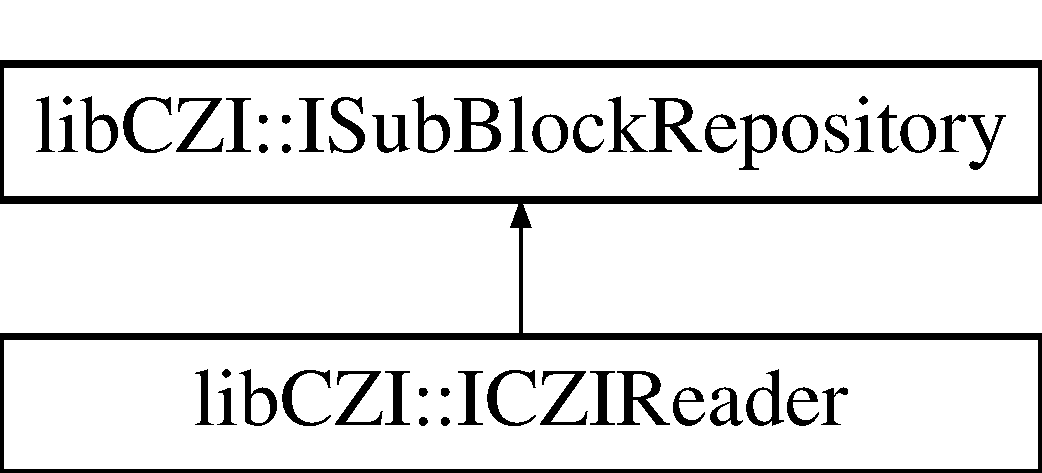
\includegraphics[height=2.000000cm]{classlib_c_z_i_1_1_i_sub_block_repository}
\end{center}
\end{figure}
\subsection*{Public Member Functions}
\begin{DoxyCompactItemize}
\item 
virtual void \hyperlink{classlib_c_z_i_1_1_i_sub_block_repository_a986ec9360cafdbadafdea9b8b5528ac3}{Enumerate\+Sub\+Blocks} (std\+::function$<$ bool(int index, const \hyperlink{structlib_c_z_i_1_1_sub_block_info}{Sub\+Block\+Info} \&info)$>$ func\+Enum)=0
\item 
virtual void \hyperlink{classlib_c_z_i_1_1_i_sub_block_repository_abf5c6fe4c21dde7079ac9c5aa04a760f}{Enum\+Subset} (const \hyperlink{classlib_c_z_i_1_1_i_dim_coordinate}{I\+Dim\+Coordinate} $\ast$plane\+Coordinate, const \hyperlink{structlib_c_z_i_1_1_int_rect}{Int\+Rect} $\ast$roi, bool only\+Layer0, std\+::function$<$ bool(int index, const \hyperlink{structlib_c_z_i_1_1_sub_block_info}{Sub\+Block\+Info} \&info)$>$ func\+Enum)=0
\item 
virtual std\+::shared\+\_\+ptr$<$ \hyperlink{classlib_c_z_i_1_1_i_sub_block}{I\+Sub\+Block} $>$ \hyperlink{classlib_c_z_i_1_1_i_sub_block_repository_afd2d9c375554492cf499c97ae49aa50b}{Read\+Sub\+Block} (int index)=0
\item 
virtual bool \hyperlink{classlib_c_z_i_1_1_i_sub_block_repository_ae557269ff1dcc03bacc21610b17d2104}{Try\+Get\+Sub\+Block\+Info\+Of\+Arbitrary\+Sub\+Block\+In\+Channel} (int channel\+Index, \hyperlink{structlib_c_z_i_1_1_sub_block_info}{Sub\+Block\+Info} \&info)=0
\item 
virtual \hyperlink{structlib_c_z_i_1_1_sub_block_statistics}{Sub\+Block\+Statistics} \hyperlink{classlib_c_z_i_1_1_i_sub_block_repository_a6e44c1a929a27036ef77195d516dd719}{Get\+Statistics} ()=0
\item 
virtual \hyperlink{structlib_c_z_i_1_1_pyramid_statistics}{Pyramid\+Statistics} \hyperlink{classlib_c_z_i_1_1_i_sub_block_repository_ab2ce65ddad39daae9ec51ea17f6fbbcf}{Get\+Pyramid\+Statistics} ()=0
\end{DoxyCompactItemize}


\subsection{Detailed Description}
Interface for sub-\/block repository. This interface is used to access the sub-\/blocks in a C\+Z\+I-\/file. 

\subsection{Member Function Documentation}
\mbox{\Hypertarget{classlib_c_z_i_1_1_i_sub_block_repository_a986ec9360cafdbadafdea9b8b5528ac3}\label{classlib_c_z_i_1_1_i_sub_block_repository_a986ec9360cafdbadafdea9b8b5528ac3}} 
\index{lib\+C\+Z\+I\+::\+I\+Sub\+Block\+Repository@{lib\+C\+Z\+I\+::\+I\+Sub\+Block\+Repository}!Enumerate\+Sub\+Blocks@{Enumerate\+Sub\+Blocks}}
\index{Enumerate\+Sub\+Blocks@{Enumerate\+Sub\+Blocks}!lib\+C\+Z\+I\+::\+I\+Sub\+Block\+Repository@{lib\+C\+Z\+I\+::\+I\+Sub\+Block\+Repository}}
\subsubsection{\texorpdfstring{Enumerate\+Sub\+Blocks()}{EnumerateSubBlocks()}}
{\footnotesize\ttfamily virtual void lib\+C\+Z\+I\+::\+I\+Sub\+Block\+Repository\+::\+Enumerate\+Sub\+Blocks (\begin{DoxyParamCaption}\item[{std\+::function$<$ bool(int index, const \hyperlink{structlib_c_z_i_1_1_sub_block_info}{Sub\+Block\+Info} \&info)$>$}]{func\+Enum }\end{DoxyParamCaption})\hspace{0.3cm}{\ttfamily [pure virtual]}}

Enumerate all sub-\/blocks. 
\begin{DoxyParams}{Parameters}
{\em func\+Enum} & The functor which will be called for every sub-\/block. If the return value of the functor is true, the enumeration is continued, otherwise it is stopped. The first argument is the index of the sub-\/block and the second is providing information about the sub-\/block. \\
\hline
\end{DoxyParams}
\mbox{\Hypertarget{classlib_c_z_i_1_1_i_sub_block_repository_abf5c6fe4c21dde7079ac9c5aa04a760f}\label{classlib_c_z_i_1_1_i_sub_block_repository_abf5c6fe4c21dde7079ac9c5aa04a760f}} 
\index{lib\+C\+Z\+I\+::\+I\+Sub\+Block\+Repository@{lib\+C\+Z\+I\+::\+I\+Sub\+Block\+Repository}!Enum\+Subset@{Enum\+Subset}}
\index{Enum\+Subset@{Enum\+Subset}!lib\+C\+Z\+I\+::\+I\+Sub\+Block\+Repository@{lib\+C\+Z\+I\+::\+I\+Sub\+Block\+Repository}}
\subsubsection{\texorpdfstring{Enum\+Subset()}{EnumSubset()}}
{\footnotesize\ttfamily virtual void lib\+C\+Z\+I\+::\+I\+Sub\+Block\+Repository\+::\+Enum\+Subset (\begin{DoxyParamCaption}\item[{const \hyperlink{classlib_c_z_i_1_1_i_dim_coordinate}{I\+Dim\+Coordinate} $\ast$}]{plane\+Coordinate,  }\item[{const \hyperlink{structlib_c_z_i_1_1_int_rect}{Int\+Rect} $\ast$}]{roi,  }\item[{bool}]{only\+Layer0,  }\item[{std\+::function$<$ bool(int index, const \hyperlink{structlib_c_z_i_1_1_sub_block_info}{Sub\+Block\+Info} \&info)$>$}]{func\+Enum }\end{DoxyParamCaption})\hspace{0.3cm}{\ttfamily [pure virtual]}}

Enumerate the subset of sub-\/blocks defined by the parameters. 
\begin{DoxyParams}{Parameters}
{\em plane\+Coordinate} & The plane coordinate. Only sub-\/blocks on this plane will be considered. \\
\hline
{\em roi} & The R\+OI -\/ only sub-\/blocks which intersects with this R\+OI will be considered. \\
\hline
{\em only\+Layer0} & If true, then only sub-\/blocks on pyramid-\/layer 0 will be considered. \\
\hline
{\em func\+Enum} & The functor which will be called for every sub-\/block. If the return value of the functor is true, the enumeration is continued, otherwise it is stopped. The first argument is the index of the sub-\/block and the second is providing information about the sub-\/block. \\
\hline
\end{DoxyParams}
\mbox{\Hypertarget{classlib_c_z_i_1_1_i_sub_block_repository_ab2ce65ddad39daae9ec51ea17f6fbbcf}\label{classlib_c_z_i_1_1_i_sub_block_repository_ab2ce65ddad39daae9ec51ea17f6fbbcf}} 
\index{lib\+C\+Z\+I\+::\+I\+Sub\+Block\+Repository@{lib\+C\+Z\+I\+::\+I\+Sub\+Block\+Repository}!Get\+Pyramid\+Statistics@{Get\+Pyramid\+Statistics}}
\index{Get\+Pyramid\+Statistics@{Get\+Pyramid\+Statistics}!lib\+C\+Z\+I\+::\+I\+Sub\+Block\+Repository@{lib\+C\+Z\+I\+::\+I\+Sub\+Block\+Repository}}
\subsubsection{\texorpdfstring{Get\+Pyramid\+Statistics()}{GetPyramidStatistics()}}
{\footnotesize\ttfamily virtual \hyperlink{structlib_c_z_i_1_1_pyramid_statistics}{Pyramid\+Statistics} lib\+C\+Z\+I\+::\+I\+Sub\+Block\+Repository\+::\+Get\+Pyramid\+Statistics (\begin{DoxyParamCaption}{ }\end{DoxyParamCaption})\hspace{0.3cm}{\ttfamily [pure virtual]}}

Gets the statistics about the pyramid-\/layers. This information is constructed from all T, Z, C, ... Pyramids are constructed per scene in C\+ZI.

\begin{DoxyReturn}{Returns}
The pyramid statistics. 
\end{DoxyReturn}
\mbox{\Hypertarget{classlib_c_z_i_1_1_i_sub_block_repository_a6e44c1a929a27036ef77195d516dd719}\label{classlib_c_z_i_1_1_i_sub_block_repository_a6e44c1a929a27036ef77195d516dd719}} 
\index{lib\+C\+Z\+I\+::\+I\+Sub\+Block\+Repository@{lib\+C\+Z\+I\+::\+I\+Sub\+Block\+Repository}!Get\+Statistics@{Get\+Statistics}}
\index{Get\+Statistics@{Get\+Statistics}!lib\+C\+Z\+I\+::\+I\+Sub\+Block\+Repository@{lib\+C\+Z\+I\+::\+I\+Sub\+Block\+Repository}}
\subsubsection{\texorpdfstring{Get\+Statistics()}{GetStatistics()}}
{\footnotesize\ttfamily virtual \hyperlink{structlib_c_z_i_1_1_sub_block_statistics}{Sub\+Block\+Statistics} lib\+C\+Z\+I\+::\+I\+Sub\+Block\+Repository\+::\+Get\+Statistics (\begin{DoxyParamCaption}{ }\end{DoxyParamCaption})\hspace{0.3cm}{\ttfamily [pure virtual]}}

Gets the statistics about the sub-\/blocks (determined from examining all sub-\/blocks). \begin{DoxyReturn}{Returns}
The sub-\/block statistics. 
\end{DoxyReturn}
\mbox{\Hypertarget{classlib_c_z_i_1_1_i_sub_block_repository_afd2d9c375554492cf499c97ae49aa50b}\label{classlib_c_z_i_1_1_i_sub_block_repository_afd2d9c375554492cf499c97ae49aa50b}} 
\index{lib\+C\+Z\+I\+::\+I\+Sub\+Block\+Repository@{lib\+C\+Z\+I\+::\+I\+Sub\+Block\+Repository}!Read\+Sub\+Block@{Read\+Sub\+Block}}
\index{Read\+Sub\+Block@{Read\+Sub\+Block}!lib\+C\+Z\+I\+::\+I\+Sub\+Block\+Repository@{lib\+C\+Z\+I\+::\+I\+Sub\+Block\+Repository}}
\subsubsection{\texorpdfstring{Read\+Sub\+Block()}{ReadSubBlock()}}
{\footnotesize\ttfamily virtual std\+::shared\+\_\+ptr$<$\hyperlink{classlib_c_z_i_1_1_i_sub_block}{I\+Sub\+Block}$>$ lib\+C\+Z\+I\+::\+I\+Sub\+Block\+Repository\+::\+Read\+Sub\+Block (\begin{DoxyParamCaption}\item[{int}]{index }\end{DoxyParamCaption})\hspace{0.3cm}{\ttfamily [pure virtual]}}

Reads the sub-\/block identified by the specified index. If there is no sub-\/block present (for the specified index) then an empty shared\+\_\+ptr is returned. If a different kind of problem occurs (e. g. I/O error or corrupted data) an exception is thrown. 
\begin{DoxyParams}{Parameters}
{\em index} & Index of the sub-\/block (as reported by the Enumerate-\/methods). \\
\hline
\end{DoxyParams}
\begin{DoxyReturn}{Returns}
If successful, the sub-\/block object; otherwise an empty shared\+\_\+ptr. 
\end{DoxyReturn}
\mbox{\Hypertarget{classlib_c_z_i_1_1_i_sub_block_repository_ae557269ff1dcc03bacc21610b17d2104}\label{classlib_c_z_i_1_1_i_sub_block_repository_ae557269ff1dcc03bacc21610b17d2104}} 
\index{lib\+C\+Z\+I\+::\+I\+Sub\+Block\+Repository@{lib\+C\+Z\+I\+::\+I\+Sub\+Block\+Repository}!Try\+Get\+Sub\+Block\+Info\+Of\+Arbitrary\+Sub\+Block\+In\+Channel@{Try\+Get\+Sub\+Block\+Info\+Of\+Arbitrary\+Sub\+Block\+In\+Channel}}
\index{Try\+Get\+Sub\+Block\+Info\+Of\+Arbitrary\+Sub\+Block\+In\+Channel@{Try\+Get\+Sub\+Block\+Info\+Of\+Arbitrary\+Sub\+Block\+In\+Channel}!lib\+C\+Z\+I\+::\+I\+Sub\+Block\+Repository@{lib\+C\+Z\+I\+::\+I\+Sub\+Block\+Repository}}
\subsubsection{\texorpdfstring{Try\+Get\+Sub\+Block\+Info\+Of\+Arbitrary\+Sub\+Block\+In\+Channel()}{TryGetSubBlockInfoOfArbitrarySubBlockInChannel()}}
{\footnotesize\ttfamily virtual bool lib\+C\+Z\+I\+::\+I\+Sub\+Block\+Repository\+::\+Try\+Get\+Sub\+Block\+Info\+Of\+Arbitrary\+Sub\+Block\+In\+Channel (\begin{DoxyParamCaption}\item[{int}]{channel\+Index,  }\item[{\hyperlink{structlib_c_z_i_1_1_sub_block_info}{Sub\+Block\+Info} \&}]{info }\end{DoxyParamCaption})\hspace{0.3cm}{\ttfamily [pure virtual]}}

Attempts to get subblock information of an arbitrary subblock in of the specified channel. The purpose is that it is quite often necessary to determine the pixeltype of a channel -\/ and if we do not want to/cannot rely on metadata for determining this, then the obvious way is to look at an (arbitrary) subblock. In order to allow the repository to have this information available fast (i. e. cached) we introduce a specific method for this purpose. A cornerstone case is when no subblock has a channel-\/index -\/ the rule is\+: if no subblock has channel-\/ information, then a channel\+Index of 0 fits. Otherwise a subblock is a match if the channel-\/ index is an exact match. 
\begin{DoxyParams}[1]{Parameters}
 & {\em channel\+Index} & The channel index. \\
\hline
\mbox{\tt out}  & {\em info} & The sub-\/block information (will be set only if the method is successful). \\
\hline
\end{DoxyParams}
\begin{DoxyReturn}{Returns}
true if it succeeds, false if it fails. 
\end{DoxyReturn}


The documentation for this class was generated from the following file\+:\begin{DoxyCompactItemize}
\item 
lib\+C\+Z\+I/lib\+C\+Z\+I.\+h\end{DoxyCompactItemize}

\hypertarget{classlib_c_z_i_1_1_i_xml_node_read}{}\section{lib\+C\+ZI\+:\+:I\+Xml\+Node\+Read Class Reference}
\label{classlib_c_z_i_1_1_i_xml_node_read}\index{lib\+C\+Z\+I\+::\+I\+Xml\+Node\+Read@{lib\+C\+Z\+I\+::\+I\+Xml\+Node\+Read}}


This interface provides read-\/only access to an X\+M\+L-\/node.  




{\ttfamily \#include $<$lib\+C\+Z\+I\+\_\+\+Metadata.\+h$>$}

Inheritance diagram for lib\+C\+ZI\+:\+:I\+Xml\+Node\+Read\+:\begin{figure}[H]
\begin{center}
\leavevmode
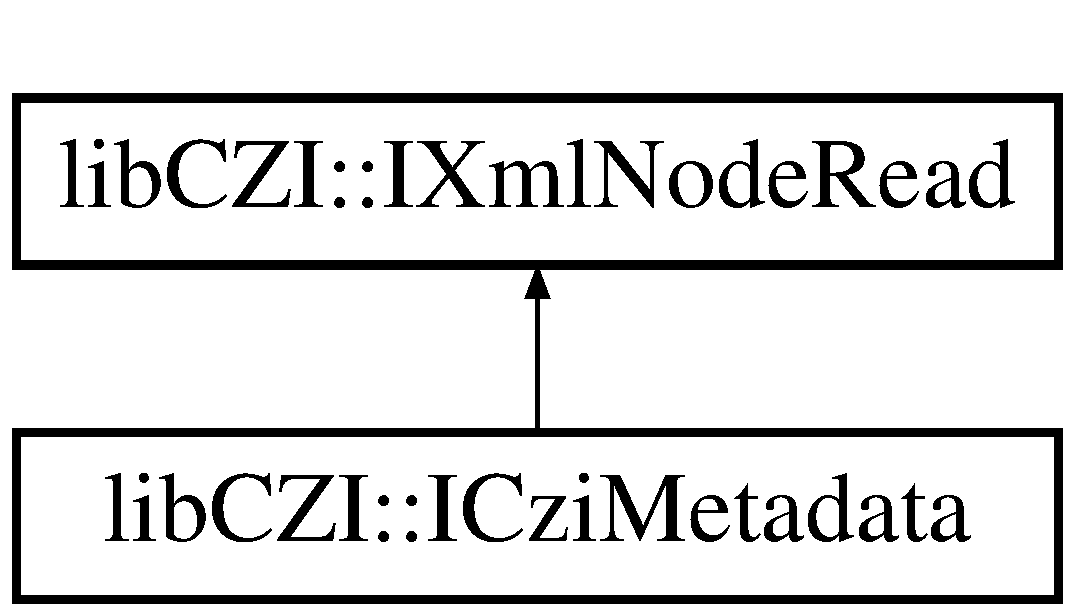
\includegraphics[height=2.000000cm]{classlib_c_z_i_1_1_i_xml_node_read}
\end{center}
\end{figure}
\subsection*{Public Member Functions}
\begin{DoxyCompactItemize}
\item 
virtual std\+::wstring \hyperlink{classlib_c_z_i_1_1_i_xml_node_read_a7a17744c795303a9c446b5ccf850a90c}{Name} () const =0
\item 
virtual bool \hyperlink{classlib_c_z_i_1_1_i_xml_node_read_a7cf31fe7e079358d5436289ee678e0df}{Try\+Get\+Attribute} (const wchar\+\_\+t $\ast$attribute\+Name, std\+::wstring $\ast$attrib\+Value) const =0
\item 
virtual void \hyperlink{classlib_c_z_i_1_1_i_xml_node_read_afe7294913f033998c7a0bb695d795c0f}{Enum\+Attributes} (const std\+::function$<$ bool(const std\+::wstring \&attrib\+Name, const std\+::wstring \&attrib\+Value)$>$ \&enum\+Func) const =0
\item 
virtual bool \hyperlink{classlib_c_z_i_1_1_i_xml_node_read_ab09530bf1a4633c499660da018bc0d89}{Try\+Get\+Value} (std\+::wstring $\ast$value) const =0
\item 
virtual std\+::shared\+\_\+ptr$<$ \hyperlink{classlib_c_z_i_1_1_i_xml_node_read}{I\+Xml\+Node\+Read} $>$ \hyperlink{classlib_c_z_i_1_1_i_xml_node_read_a4e14de646b5624daf11b16ba42094c74}{Get\+Child\+Node\+Readonly} (const char $\ast$path)=0
\item 
virtual void \hyperlink{classlib_c_z_i_1_1_i_xml_node_read_a70385059cfda44a6f2d590a9a8d6ac3e}{Enum\+Children} (std\+::function$<$ bool(std\+::shared\+\_\+ptr$<$ \hyperlink{classlib_c_z_i_1_1_i_xml_node_read}{I\+Xml\+Node\+Read} $>$)$>$ enum\+Children)=0
\item 
bool \hyperlink{classlib_c_z_i_1_1_i_xml_node_read_a3bb9226ebe823d70968e694407f90bc7}{Try\+Get\+Value\+As\+Double} (double $\ast$p)
\item 
bool \hyperlink{classlib_c_z_i_1_1_i_xml_node_read_af3070ab11416f7658e198d8cd89210c0}{Try\+Get\+Value\+As\+Float} (float $\ast$p)
\item 
bool \hyperlink{classlib_c_z_i_1_1_i_xml_node_read_ad03686b294d2271dfa1a44c88c0751bc}{Try\+Get\+Value\+As\+Int32} (std\+::int32\+\_\+t $\ast$p)
\item 
bool \hyperlink{classlib_c_z_i_1_1_i_xml_node_read_a0cbe508500066393c05e5ebdfc3c7df7}{Try\+Get\+Value\+As\+U\+Int32} (std\+::uint32\+\_\+t $\ast$p)
\item 
bool \hyperlink{classlib_c_z_i_1_1_i_xml_node_read_adbf74c7628e88a54791b315c12b176bf}{Try\+Get\+Value\+As\+Int64} (std\+::int64\+\_\+t $\ast$p)
\item 
bool \hyperlink{classlib_c_z_i_1_1_i_xml_node_read_a6a250a2916f16985eff64b7a82ed2d99}{Try\+Get\+Value\+As\+U\+Int64} (std\+::uint64\+\_\+t $\ast$p)
\item 
bool \hyperlink{classlib_c_z_i_1_1_i_xml_node_read_a2d12c91c7ff8ef3b822d623f6c04b14f}{Try\+Get\+Value\+As\+Bool} (bool $\ast$p)
\end{DoxyCompactItemize}


\subsection{Detailed Description}
This interface provides read-\/only access to an X\+M\+L-\/node. 

\subsection{Member Function Documentation}
\mbox{\Hypertarget{classlib_c_z_i_1_1_i_xml_node_read_afe7294913f033998c7a0bb695d795c0f}\label{classlib_c_z_i_1_1_i_xml_node_read_afe7294913f033998c7a0bb695d795c0f}} 
\index{lib\+C\+Z\+I\+::\+I\+Xml\+Node\+Read@{lib\+C\+Z\+I\+::\+I\+Xml\+Node\+Read}!Enum\+Attributes@{Enum\+Attributes}}
\index{Enum\+Attributes@{Enum\+Attributes}!lib\+C\+Z\+I\+::\+I\+Xml\+Node\+Read@{lib\+C\+Z\+I\+::\+I\+Xml\+Node\+Read}}
\subsubsection{\texorpdfstring{Enum\+Attributes()}{EnumAttributes()}}
{\footnotesize\ttfamily virtual void lib\+C\+Z\+I\+::\+I\+Xml\+Node\+Read\+::\+Enum\+Attributes (\begin{DoxyParamCaption}\item[{const std\+::function$<$ bool(const std\+::wstring \&attrib\+Name, const std\+::wstring \&attrib\+Value)$>$ \&}]{enum\+Func }\end{DoxyParamCaption}) const\hspace{0.3cm}{\ttfamily [pure virtual]}}

Enumerate the attributes in the node. The attribute-\/name and their respective value will be passed to the specified functor.


\begin{DoxyParams}{Parameters}
{\em enum\+Func} & The enumeration function. If the function returns false, the enumeration will be cancelled immediately. \\
\hline
\end{DoxyParams}
\mbox{\Hypertarget{classlib_c_z_i_1_1_i_xml_node_read_a70385059cfda44a6f2d590a9a8d6ac3e}\label{classlib_c_z_i_1_1_i_xml_node_read_a70385059cfda44a6f2d590a9a8d6ac3e}} 
\index{lib\+C\+Z\+I\+::\+I\+Xml\+Node\+Read@{lib\+C\+Z\+I\+::\+I\+Xml\+Node\+Read}!Enum\+Children@{Enum\+Children}}
\index{Enum\+Children@{Enum\+Children}!lib\+C\+Z\+I\+::\+I\+Xml\+Node\+Read@{lib\+C\+Z\+I\+::\+I\+Xml\+Node\+Read}}
\subsubsection{\texorpdfstring{Enum\+Children()}{EnumChildren()}}
{\footnotesize\ttfamily virtual void lib\+C\+Z\+I\+::\+I\+Xml\+Node\+Read\+::\+Enum\+Children (\begin{DoxyParamCaption}\item[{std\+::function$<$ bool(std\+::shared\+\_\+ptr$<$ \hyperlink{classlib_c_z_i_1_1_i_xml_node_read}{I\+Xml\+Node\+Read} $>$)$>$}]{enum\+Children }\end{DoxyParamCaption})\hspace{0.3cm}{\ttfamily [pure virtual]}}

Enumerate the children of the node. The functor will be called until there are no more children or if the function return false. 
\begin{DoxyParams}{Parameters}
{\em enum\+Children} & The function to be called with the children nodes. \\
\hline
\end{DoxyParams}
\mbox{\Hypertarget{classlib_c_z_i_1_1_i_xml_node_read_a4e14de646b5624daf11b16ba42094c74}\label{classlib_c_z_i_1_1_i_xml_node_read_a4e14de646b5624daf11b16ba42094c74}} 
\index{lib\+C\+Z\+I\+::\+I\+Xml\+Node\+Read@{lib\+C\+Z\+I\+::\+I\+Xml\+Node\+Read}!Get\+Child\+Node\+Readonly@{Get\+Child\+Node\+Readonly}}
\index{Get\+Child\+Node\+Readonly@{Get\+Child\+Node\+Readonly}!lib\+C\+Z\+I\+::\+I\+Xml\+Node\+Read@{lib\+C\+Z\+I\+::\+I\+Xml\+Node\+Read}}
\subsubsection{\texorpdfstring{Get\+Child\+Node\+Readonly()}{GetChildNodeReadonly()}}
{\footnotesize\ttfamily virtual std\+::shared\+\_\+ptr$<$\hyperlink{classlib_c_z_i_1_1_i_xml_node_read}{I\+Xml\+Node\+Read}$>$ lib\+C\+Z\+I\+::\+I\+Xml\+Node\+Read\+::\+Get\+Child\+Node\+Readonly (\begin{DoxyParamCaption}\item[{const char $\ast$}]{path }\end{DoxyParamCaption})\hspace{0.3cm}{\ttfamily [pure virtual]}}

Gets a child node for the specified path/attribute specification if it exists. Otherwise, a nullptr is returned. The path is specified as node-\/names separated by slashes. At path \char`\"{}\+A/\+B/\+C\char`\"{} selects (or creates) a node-\/structure like this 
\begin{DoxyCode}
<A>
  <B>
    <C/>
  </B>
</A>
\end{DoxyCode}
 Attributes can be specified with a node, in the form \textquotesingle{}Node\+Name\mbox{[}attr1=abc,attr2=xyz\mbox{]}\textquotesingle{}. This will search for nodes with the specified attributes, and if not found, create one. In this example \char`\"{}\+A/\+B\mbox{[}\+Id=ab,\+Name=xy\mbox{]}/\+C\char`\"{} we will get 
\begin{DoxyCode}
<A>
  <B Id="ab" Name="xy">
    <C/>
  </B>
</A>
\end{DoxyCode}
 
\begin{DoxyParams}{Parameters}
{\em path} & The path (in U\+T\+F8-\/encoding). \\
\hline
\end{DoxyParams}
\begin{DoxyReturn}{Returns}
Either the requested node if it exists or nullptr. 
\end{DoxyReturn}
\mbox{\Hypertarget{classlib_c_z_i_1_1_i_xml_node_read_a7a17744c795303a9c446b5ccf850a90c}\label{classlib_c_z_i_1_1_i_xml_node_read_a7a17744c795303a9c446b5ccf850a90c}} 
\index{lib\+C\+Z\+I\+::\+I\+Xml\+Node\+Read@{lib\+C\+Z\+I\+::\+I\+Xml\+Node\+Read}!Name@{Name}}
\index{Name@{Name}!lib\+C\+Z\+I\+::\+I\+Xml\+Node\+Read@{lib\+C\+Z\+I\+::\+I\+Xml\+Node\+Read}}
\subsubsection{\texorpdfstring{Name()}{Name()}}
{\footnotesize\ttfamily virtual std\+::wstring lib\+C\+Z\+I\+::\+I\+Xml\+Node\+Read\+::\+Name (\begin{DoxyParamCaption}{ }\end{DoxyParamCaption}) const\hspace{0.3cm}{\ttfamily [pure virtual]}}

Gets the name of the node. \begin{DoxyReturn}{Returns}
The name of the node. 
\end{DoxyReturn}
\mbox{\Hypertarget{classlib_c_z_i_1_1_i_xml_node_read_a7cf31fe7e079358d5436289ee678e0df}\label{classlib_c_z_i_1_1_i_xml_node_read_a7cf31fe7e079358d5436289ee678e0df}} 
\index{lib\+C\+Z\+I\+::\+I\+Xml\+Node\+Read@{lib\+C\+Z\+I\+::\+I\+Xml\+Node\+Read}!Try\+Get\+Attribute@{Try\+Get\+Attribute}}
\index{Try\+Get\+Attribute@{Try\+Get\+Attribute}!lib\+C\+Z\+I\+::\+I\+Xml\+Node\+Read@{lib\+C\+Z\+I\+::\+I\+Xml\+Node\+Read}}
\subsubsection{\texorpdfstring{Try\+Get\+Attribute()}{TryGetAttribute()}}
{\footnotesize\ttfamily virtual bool lib\+C\+Z\+I\+::\+I\+Xml\+Node\+Read\+::\+Try\+Get\+Attribute (\begin{DoxyParamCaption}\item[{const wchar\+\_\+t $\ast$}]{attribute\+Name,  }\item[{std\+::wstring $\ast$}]{attrib\+Value }\end{DoxyParamCaption}) const\hspace{0.3cm}{\ttfamily [pure virtual]}}

Attempts to get the attribute with the name specified by \char`\"{}attribute\+Name\char`\"{}. If it exists, the value is stored in \char`\"{}attrib\+Value\char`\"{} (if it is non-\/null) and the return value is true. Otherwise, the return value is false.


\begin{DoxyParams}[1]{Parameters}
 & {\em attribute\+Name} & Name of the attribute. \\
\hline
\mbox{\tt out}  & {\em attrib\+Value} & If non-\/null, the attribute value will be put here (if the attribute exists).\\
\hline
\end{DoxyParams}
\begin{DoxyReturn}{Returns}
True if it succeeds, false if it fails. 
\end{DoxyReturn}
\mbox{\Hypertarget{classlib_c_z_i_1_1_i_xml_node_read_ab09530bf1a4633c499660da018bc0d89}\label{classlib_c_z_i_1_1_i_xml_node_read_ab09530bf1a4633c499660da018bc0d89}} 
\index{lib\+C\+Z\+I\+::\+I\+Xml\+Node\+Read@{lib\+C\+Z\+I\+::\+I\+Xml\+Node\+Read}!Try\+Get\+Value@{Try\+Get\+Value}}
\index{Try\+Get\+Value@{Try\+Get\+Value}!lib\+C\+Z\+I\+::\+I\+Xml\+Node\+Read@{lib\+C\+Z\+I\+::\+I\+Xml\+Node\+Read}}
\subsubsection{\texorpdfstring{Try\+Get\+Value()}{TryGetValue()}}
{\footnotesize\ttfamily virtual bool lib\+C\+Z\+I\+::\+I\+Xml\+Node\+Read\+::\+Try\+Get\+Value (\begin{DoxyParamCaption}\item[{std\+::wstring $\ast$}]{value }\end{DoxyParamCaption}) const\hspace{0.3cm}{\ttfamily [pure virtual]}}

Attempts to get value of the X\+M\+L-\/node. If the specified pointer \char`\"{}value\char`\"{} is non-\/null, the value will be put there.


\begin{DoxyParams}[1]{Parameters}
\mbox{\tt out}  & {\em value} & If non-\/null, the value of the X\+M\+L-\/node will be put here (if successful).\\
\hline
\end{DoxyParams}
\begin{DoxyReturn}{Returns}
True if it succeeds, false if it fails. 
\end{DoxyReturn}
\mbox{\Hypertarget{classlib_c_z_i_1_1_i_xml_node_read_a2d12c91c7ff8ef3b822d623f6c04b14f}\label{classlib_c_z_i_1_1_i_xml_node_read_a2d12c91c7ff8ef3b822d623f6c04b14f}} 
\index{lib\+C\+Z\+I\+::\+I\+Xml\+Node\+Read@{lib\+C\+Z\+I\+::\+I\+Xml\+Node\+Read}!Try\+Get\+Value\+As\+Bool@{Try\+Get\+Value\+As\+Bool}}
\index{Try\+Get\+Value\+As\+Bool@{Try\+Get\+Value\+As\+Bool}!lib\+C\+Z\+I\+::\+I\+Xml\+Node\+Read@{lib\+C\+Z\+I\+::\+I\+Xml\+Node\+Read}}
\subsubsection{\texorpdfstring{Try\+Get\+Value\+As\+Bool()}{TryGetValueAsBool()}}
{\footnotesize\ttfamily bool lib\+C\+Z\+I\+::\+I\+Xml\+Node\+Read\+::\+Try\+Get\+Value\+As\+Bool (\begin{DoxyParamCaption}\item[{bool $\ast$}]{p }\end{DoxyParamCaption})}

Attempts to get value of this node as an unsigned long integer (64-\/bit). Valid values for true are\+: \char`\"{}true\char`\"{}, \char`\"{}yes\char`\"{} or \char`\"{}1\char`\"{}; valid values for false are \char`\"{}false\char`\"{}, \char`\"{}no\char`\"{} or \char`\"{}0\char`\"{} (case insensitive comparison). 
\begin{DoxyParams}[1]{Parameters}
\mbox{\tt in,out}  & {\em p} & If non-\/null, a pointer to a bool to store the result in. \\
\hline
\end{DoxyParams}
\begin{DoxyReturn}{Returns}
True if it succeeds, false if it fails. 
\end{DoxyReturn}
\mbox{\Hypertarget{classlib_c_z_i_1_1_i_xml_node_read_a3bb9226ebe823d70968e694407f90bc7}\label{classlib_c_z_i_1_1_i_xml_node_read_a3bb9226ebe823d70968e694407f90bc7}} 
\index{lib\+C\+Z\+I\+::\+I\+Xml\+Node\+Read@{lib\+C\+Z\+I\+::\+I\+Xml\+Node\+Read}!Try\+Get\+Value\+As\+Double@{Try\+Get\+Value\+As\+Double}}
\index{Try\+Get\+Value\+As\+Double@{Try\+Get\+Value\+As\+Double}!lib\+C\+Z\+I\+::\+I\+Xml\+Node\+Read@{lib\+C\+Z\+I\+::\+I\+Xml\+Node\+Read}}
\subsubsection{\texorpdfstring{Try\+Get\+Value\+As\+Double()}{TryGetValueAsDouble()}}
{\footnotesize\ttfamily bool lib\+C\+Z\+I\+::\+I\+Xml\+Node\+Read\+::\+Try\+Get\+Value\+As\+Double (\begin{DoxyParamCaption}\item[{double $\ast$}]{p }\end{DoxyParamCaption})}

Attempts to get value of this node as a double. If the text does not parse correctly (or is empty), we return false. 
\begin{DoxyParams}[1]{Parameters}
\mbox{\tt in,out}  & {\em p} & If non-\/null, a pointer to a double to store the result in. \\
\hline
\end{DoxyParams}
\begin{DoxyReturn}{Returns}
True if it succeeds, false if it fails. 
\end{DoxyReturn}
\mbox{\Hypertarget{classlib_c_z_i_1_1_i_xml_node_read_af3070ab11416f7658e198d8cd89210c0}\label{classlib_c_z_i_1_1_i_xml_node_read_af3070ab11416f7658e198d8cd89210c0}} 
\index{lib\+C\+Z\+I\+::\+I\+Xml\+Node\+Read@{lib\+C\+Z\+I\+::\+I\+Xml\+Node\+Read}!Try\+Get\+Value\+As\+Float@{Try\+Get\+Value\+As\+Float}}
\index{Try\+Get\+Value\+As\+Float@{Try\+Get\+Value\+As\+Float}!lib\+C\+Z\+I\+::\+I\+Xml\+Node\+Read@{lib\+C\+Z\+I\+::\+I\+Xml\+Node\+Read}}
\subsubsection{\texorpdfstring{Try\+Get\+Value\+As\+Float()}{TryGetValueAsFloat()}}
{\footnotesize\ttfamily bool lib\+C\+Z\+I\+::\+I\+Xml\+Node\+Read\+::\+Try\+Get\+Value\+As\+Float (\begin{DoxyParamCaption}\item[{float $\ast$}]{p }\end{DoxyParamCaption})}

Attempts to get value of this node as a float. If the text does not parse correctly (or is empty), we return false. 
\begin{DoxyParams}[1]{Parameters}
\mbox{\tt in,out}  & {\em p} & If non-\/null, a pointer to a float to store the result in. \\
\hline
\end{DoxyParams}
\begin{DoxyReturn}{Returns}
True if it succeeds, false if it fails. 
\end{DoxyReturn}
\mbox{\Hypertarget{classlib_c_z_i_1_1_i_xml_node_read_ad03686b294d2271dfa1a44c88c0751bc}\label{classlib_c_z_i_1_1_i_xml_node_read_ad03686b294d2271dfa1a44c88c0751bc}} 
\index{lib\+C\+Z\+I\+::\+I\+Xml\+Node\+Read@{lib\+C\+Z\+I\+::\+I\+Xml\+Node\+Read}!Try\+Get\+Value\+As\+Int32@{Try\+Get\+Value\+As\+Int32}}
\index{Try\+Get\+Value\+As\+Int32@{Try\+Get\+Value\+As\+Int32}!lib\+C\+Z\+I\+::\+I\+Xml\+Node\+Read@{lib\+C\+Z\+I\+::\+I\+Xml\+Node\+Read}}
\subsubsection{\texorpdfstring{Try\+Get\+Value\+As\+Int32()}{TryGetValueAsInt32()}}
{\footnotesize\ttfamily bool lib\+C\+Z\+I\+::\+I\+Xml\+Node\+Read\+::\+Try\+Get\+Value\+As\+Int32 (\begin{DoxyParamCaption}\item[{std\+::int32\+\_\+t $\ast$}]{p }\end{DoxyParamCaption})}

Attempts to get value of this node as an integer (32-\/bit). If the text does not parse correctly (or is empty), we return false. 
\begin{DoxyParams}[1]{Parameters}
\mbox{\tt in,out}  & {\em p} & If non-\/null, a pointer to a integer to store the result in. \\
\hline
\end{DoxyParams}
\begin{DoxyReturn}{Returns}
True if it succeeds, false if it fails. 
\end{DoxyReturn}
\mbox{\Hypertarget{classlib_c_z_i_1_1_i_xml_node_read_adbf74c7628e88a54791b315c12b176bf}\label{classlib_c_z_i_1_1_i_xml_node_read_adbf74c7628e88a54791b315c12b176bf}} 
\index{lib\+C\+Z\+I\+::\+I\+Xml\+Node\+Read@{lib\+C\+Z\+I\+::\+I\+Xml\+Node\+Read}!Try\+Get\+Value\+As\+Int64@{Try\+Get\+Value\+As\+Int64}}
\index{Try\+Get\+Value\+As\+Int64@{Try\+Get\+Value\+As\+Int64}!lib\+C\+Z\+I\+::\+I\+Xml\+Node\+Read@{lib\+C\+Z\+I\+::\+I\+Xml\+Node\+Read}}
\subsubsection{\texorpdfstring{Try\+Get\+Value\+As\+Int64()}{TryGetValueAsInt64()}}
{\footnotesize\ttfamily bool lib\+C\+Z\+I\+::\+I\+Xml\+Node\+Read\+::\+Try\+Get\+Value\+As\+Int64 (\begin{DoxyParamCaption}\item[{std\+::int64\+\_\+t $\ast$}]{p }\end{DoxyParamCaption})}

Attempts to get value of this node as a long integer (64-\/bit). If the text does not parse correctly (or is empty), we return false. 
\begin{DoxyParams}[1]{Parameters}
\mbox{\tt in,out}  & {\em p} & If non-\/null, a pointer to a long integer (64-\/bit) to store the result in. \\
\hline
\end{DoxyParams}
\begin{DoxyReturn}{Returns}
True if it succeeds, false if it fails. 
\end{DoxyReturn}
\mbox{\Hypertarget{classlib_c_z_i_1_1_i_xml_node_read_a0cbe508500066393c05e5ebdfc3c7df7}\label{classlib_c_z_i_1_1_i_xml_node_read_a0cbe508500066393c05e5ebdfc3c7df7}} 
\index{lib\+C\+Z\+I\+::\+I\+Xml\+Node\+Read@{lib\+C\+Z\+I\+::\+I\+Xml\+Node\+Read}!Try\+Get\+Value\+As\+U\+Int32@{Try\+Get\+Value\+As\+U\+Int32}}
\index{Try\+Get\+Value\+As\+U\+Int32@{Try\+Get\+Value\+As\+U\+Int32}!lib\+C\+Z\+I\+::\+I\+Xml\+Node\+Read@{lib\+C\+Z\+I\+::\+I\+Xml\+Node\+Read}}
\subsubsection{\texorpdfstring{Try\+Get\+Value\+As\+U\+Int32()}{TryGetValueAsUInt32()}}
{\footnotesize\ttfamily bool lib\+C\+Z\+I\+::\+I\+Xml\+Node\+Read\+::\+Try\+Get\+Value\+As\+U\+Int32 (\begin{DoxyParamCaption}\item[{std\+::uint32\+\_\+t $\ast$}]{p }\end{DoxyParamCaption})}

Attempts to get value of this node as an unsigned integer (32-\/bit). If the text does not parse correctly (or is empty), we return false. 
\begin{DoxyParams}[1]{Parameters}
\mbox{\tt in,out}  & {\em p} & If non-\/null, a pointer to an unsigned integer to store the result in. \\
\hline
\end{DoxyParams}
\begin{DoxyReturn}{Returns}
True if it succeeds, false if it fails. 
\end{DoxyReturn}
\mbox{\Hypertarget{classlib_c_z_i_1_1_i_xml_node_read_a6a250a2916f16985eff64b7a82ed2d99}\label{classlib_c_z_i_1_1_i_xml_node_read_a6a250a2916f16985eff64b7a82ed2d99}} 
\index{lib\+C\+Z\+I\+::\+I\+Xml\+Node\+Read@{lib\+C\+Z\+I\+::\+I\+Xml\+Node\+Read}!Try\+Get\+Value\+As\+U\+Int64@{Try\+Get\+Value\+As\+U\+Int64}}
\index{Try\+Get\+Value\+As\+U\+Int64@{Try\+Get\+Value\+As\+U\+Int64}!lib\+C\+Z\+I\+::\+I\+Xml\+Node\+Read@{lib\+C\+Z\+I\+::\+I\+Xml\+Node\+Read}}
\subsubsection{\texorpdfstring{Try\+Get\+Value\+As\+U\+Int64()}{TryGetValueAsUInt64()}}
{\footnotesize\ttfamily bool lib\+C\+Z\+I\+::\+I\+Xml\+Node\+Read\+::\+Try\+Get\+Value\+As\+U\+Int64 (\begin{DoxyParamCaption}\item[{std\+::uint64\+\_\+t $\ast$}]{p }\end{DoxyParamCaption})}

Attempts to get value of this node as an unsigned long integer (64-\/bit). If the text does not parse correctly (or is empty), we return false. 
\begin{DoxyParams}[1]{Parameters}
\mbox{\tt in,out}  & {\em p} & If non-\/null, a pointer to an unsigned long integer (64-\/bit) to store the result in. \\
\hline
\end{DoxyParams}
\begin{DoxyReturn}{Returns}
True if it succeeds, false if it fails. 
\end{DoxyReturn}


The documentation for this class was generated from the following file\+:\begin{DoxyCompactItemize}
\item 
lib\+C\+Z\+I/lib\+C\+Z\+I\+\_\+\+Metadata.\+h\end{DoxyCompactItemize}

\hypertarget{classlib_c_z_i_1_1_lib_c_z_i_accessor_exception}{}\section{lib\+C\+ZI\+:\+:Lib\+C\+Z\+I\+Accessor\+Exception Class Reference}
\label{classlib_c_z_i_1_1_lib_c_z_i_accessor_exception}\index{lib\+C\+Z\+I\+::\+Lib\+C\+Z\+I\+Accessor\+Exception@{lib\+C\+Z\+I\+::\+Lib\+C\+Z\+I\+Accessor\+Exception}}


Exception for signaling errors specific for accessors.  




{\ttfamily \#include $<$lib\+C\+Z\+I\+\_\+exceptions.\+h$>$}

Inheritance diagram for lib\+C\+ZI\+:\+:Lib\+C\+Z\+I\+Accessor\+Exception\+:\begin{figure}[H]
\begin{center}
\leavevmode
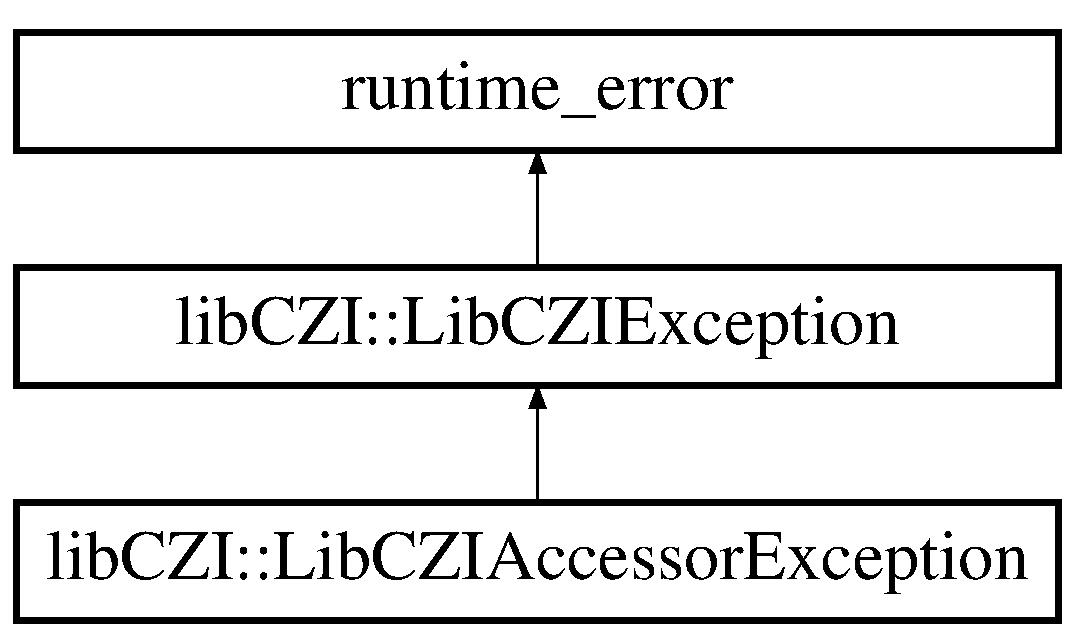
\includegraphics[height=3.000000cm]{classlib_c_z_i_1_1_lib_c_z_i_accessor_exception}
\end{center}
\end{figure}
\subsection*{Public Types}
\begin{DoxyCompactItemize}
\item 
enum \hyperlink{classlib_c_z_i_1_1_lib_c_z_i_accessor_exception_afac26a03ad8be1d8314911a58b9b08b5}{Error\+Type} \{ \hyperlink{classlib_c_z_i_1_1_lib_c_z_i_accessor_exception_afac26a03ad8be1d8314911a58b9b08b5ab9a3da346ec292af4ab30323d51475a7}{Error\+Type\+::\+Couldnt\+Determine\+Pixel\+Type}, 
\hyperlink{classlib_c_z_i_1_1_lib_c_z_i_accessor_exception_afac26a03ad8be1d8314911a58b9b08b5a6fcdc090caeade09d0efd6253932b6f5}{Error\+Type\+::\+Unspecified}
 \}\begin{DoxyCompactList}\small\item\em Values that represent error types. \end{DoxyCompactList}
\end{DoxyCompactItemize}
\subsection*{Public Member Functions}
\begin{DoxyCompactItemize}
\item 
\hyperlink{classlib_c_z_i_1_1_lib_c_z_i_accessor_exception_a4eb949381be1d9ca7e1f1b65f5fdacd0}{Lib\+C\+Z\+I\+Accessor\+Exception} (const char $\ast$sz\+Err\+Msg, \hyperlink{classlib_c_z_i_1_1_lib_c_z_i_accessor_exception_afac26a03ad8be1d8314911a58b9b08b5}{Error\+Type} error\+Type)
\item 
\hyperlink{classlib_c_z_i_1_1_lib_c_z_i_accessor_exception_afac26a03ad8be1d8314911a58b9b08b5}{Error\+Type} \hyperlink{classlib_c_z_i_1_1_lib_c_z_i_accessor_exception_a8d5241a5d61e5d2ae97a6ee4c8f3e39e}{Get\+Error\+Type} () const
\end{DoxyCompactItemize}


\subsection{Detailed Description}
Exception for signaling errors specific for accessors. 

\subsection{Member Enumeration Documentation}
\mbox{\Hypertarget{classlib_c_z_i_1_1_lib_c_z_i_accessor_exception_afac26a03ad8be1d8314911a58b9b08b5}\label{classlib_c_z_i_1_1_lib_c_z_i_accessor_exception_afac26a03ad8be1d8314911a58b9b08b5}} 
\index{lib\+C\+Z\+I\+::\+Lib\+C\+Z\+I\+Accessor\+Exception@{lib\+C\+Z\+I\+::\+Lib\+C\+Z\+I\+Accessor\+Exception}!Error\+Type@{Error\+Type}}
\index{Error\+Type@{Error\+Type}!lib\+C\+Z\+I\+::\+Lib\+C\+Z\+I\+Accessor\+Exception@{lib\+C\+Z\+I\+::\+Lib\+C\+Z\+I\+Accessor\+Exception}}
\subsubsection{\texorpdfstring{Error\+Type}{ErrorType}}
{\footnotesize\ttfamily enum \hyperlink{classlib_c_z_i_1_1_lib_c_z_i_accessor_exception_afac26a03ad8be1d8314911a58b9b08b5}{lib\+C\+Z\+I\+::\+Lib\+C\+Z\+I\+Accessor\+Exception\+::\+Error\+Type}\hspace{0.3cm}{\ttfamily [strong]}}



Values that represent error types. 

\begin{DoxyEnumFields}{Enumerator}
\raisebox{\heightof{T}}[0pt][0pt]{\index{Couldnt\+Determine\+Pixel\+Type@{Couldnt\+Determine\+Pixel\+Type}!lib\+C\+Z\+I\+::\+Lib\+C\+Z\+I\+Accessor\+Exception@{lib\+C\+Z\+I\+::\+Lib\+C\+Z\+I\+Accessor\+Exception}}\index{lib\+C\+Z\+I\+::\+Lib\+C\+Z\+I\+Accessor\+Exception@{lib\+C\+Z\+I\+::\+Lib\+C\+Z\+I\+Accessor\+Exception}!Couldnt\+Determine\+Pixel\+Type@{Couldnt\+Determine\+Pixel\+Type}}}\mbox{\Hypertarget{classlib_c_z_i_1_1_lib_c_z_i_accessor_exception_afac26a03ad8be1d8314911a58b9b08b5ab9a3da346ec292af4ab30323d51475a7}\label{classlib_c_z_i_1_1_lib_c_z_i_accessor_exception_afac26a03ad8be1d8314911a58b9b08b5ab9a3da346ec292af4ab30323d51475a7}} 
Couldnt\+Determine\+Pixel\+Type&The pixeltype could not be determined. \\
\hline

\raisebox{\heightof{T}}[0pt][0pt]{\index{Unspecified@{Unspecified}!lib\+C\+Z\+I\+::\+Lib\+C\+Z\+I\+Accessor\+Exception@{lib\+C\+Z\+I\+::\+Lib\+C\+Z\+I\+Accessor\+Exception}}\index{lib\+C\+Z\+I\+::\+Lib\+C\+Z\+I\+Accessor\+Exception@{lib\+C\+Z\+I\+::\+Lib\+C\+Z\+I\+Accessor\+Exception}!Unspecified@{Unspecified}}}\mbox{\Hypertarget{classlib_c_z_i_1_1_lib_c_z_i_accessor_exception_afac26a03ad8be1d8314911a58b9b08b5a6fcdc090caeade09d0efd6253932b6f5}\label{classlib_c_z_i_1_1_lib_c_z_i_accessor_exception_afac26a03ad8be1d8314911a58b9b08b5a6fcdc090caeade09d0efd6253932b6f5}} 
Unspecified&Unspecified error. \\
\hline

\end{DoxyEnumFields}


\subsection{Constructor \& Destructor Documentation}
\mbox{\Hypertarget{classlib_c_z_i_1_1_lib_c_z_i_accessor_exception_a4eb949381be1d9ca7e1f1b65f5fdacd0}\label{classlib_c_z_i_1_1_lib_c_z_i_accessor_exception_a4eb949381be1d9ca7e1f1b65f5fdacd0}} 
\index{lib\+C\+Z\+I\+::\+Lib\+C\+Z\+I\+Accessor\+Exception@{lib\+C\+Z\+I\+::\+Lib\+C\+Z\+I\+Accessor\+Exception}!Lib\+C\+Z\+I\+Accessor\+Exception@{Lib\+C\+Z\+I\+Accessor\+Exception}}
\index{Lib\+C\+Z\+I\+Accessor\+Exception@{Lib\+C\+Z\+I\+Accessor\+Exception}!lib\+C\+Z\+I\+::\+Lib\+C\+Z\+I\+Accessor\+Exception@{lib\+C\+Z\+I\+::\+Lib\+C\+Z\+I\+Accessor\+Exception}}
\subsubsection{\texorpdfstring{Lib\+C\+Z\+I\+Accessor\+Exception()}{LibCZIAccessorException()}}
{\footnotesize\ttfamily lib\+C\+Z\+I\+::\+Lib\+C\+Z\+I\+Accessor\+Exception\+::\+Lib\+C\+Z\+I\+Accessor\+Exception (\begin{DoxyParamCaption}\item[{const char $\ast$}]{sz\+Err\+Msg,  }\item[{\hyperlink{classlib_c_z_i_1_1_lib_c_z_i_accessor_exception_afac26a03ad8be1d8314911a58b9b08b5}{Error\+Type}}]{error\+Type }\end{DoxyParamCaption})\hspace{0.3cm}{\ttfamily [inline]}}

Constructor for the \hyperlink{classlib_c_z_i_1_1_lib_c_z_i_accessor_exception}{Lib\+C\+Z\+I\+Accessor\+Exception}. 
\begin{DoxyParams}{Parameters}
{\em sz\+Err\+Msg} & Message describing the error. This type is used to signal error that are specific for accessors. \\
\hline
{\em error\+Type} & Type of the error. \\
\hline
\end{DoxyParams}


\subsection{Member Function Documentation}
\mbox{\Hypertarget{classlib_c_z_i_1_1_lib_c_z_i_accessor_exception_a8d5241a5d61e5d2ae97a6ee4c8f3e39e}\label{classlib_c_z_i_1_1_lib_c_z_i_accessor_exception_a8d5241a5d61e5d2ae97a6ee4c8f3e39e}} 
\index{lib\+C\+Z\+I\+::\+Lib\+C\+Z\+I\+Accessor\+Exception@{lib\+C\+Z\+I\+::\+Lib\+C\+Z\+I\+Accessor\+Exception}!Get\+Error\+Type@{Get\+Error\+Type}}
\index{Get\+Error\+Type@{Get\+Error\+Type}!lib\+C\+Z\+I\+::\+Lib\+C\+Z\+I\+Accessor\+Exception@{lib\+C\+Z\+I\+::\+Lib\+C\+Z\+I\+Accessor\+Exception}}
\subsubsection{\texorpdfstring{Get\+Error\+Type()}{GetErrorType()}}
{\footnotesize\ttfamily \hyperlink{classlib_c_z_i_1_1_lib_c_z_i_accessor_exception_afac26a03ad8be1d8314911a58b9b08b5}{Error\+Type} lib\+C\+Z\+I\+::\+Lib\+C\+Z\+I\+Accessor\+Exception\+::\+Get\+Error\+Type (\begin{DoxyParamCaption}{ }\end{DoxyParamCaption}) const\hspace{0.3cm}{\ttfamily [inline]}}

Gets error type. \begin{DoxyReturn}{Returns}
The error type. 
\end{DoxyReturn}


The documentation for this class was generated from the following file\+:\begin{DoxyCompactItemize}
\item 
lib\+C\+Z\+I/lib\+C\+Z\+I\+\_\+exceptions.\+h\end{DoxyCompactItemize}

\hypertarget{structlib_c_z_i_1_1_lib_c_z_i_c_z_i_parse_exception}{}\section{lib\+C\+ZI\+:\+:Lib\+C\+Z\+I\+C\+Z\+I\+Parse\+Exception Struct Reference}
\label{structlib_c_z_i_1_1_lib_c_z_i_c_z_i_parse_exception}\index{lib\+C\+Z\+I\+::\+Lib\+C\+Z\+I\+C\+Z\+I\+Parse\+Exception@{lib\+C\+Z\+I\+::\+Lib\+C\+Z\+I\+C\+Z\+I\+Parse\+Exception}}


Exception for signaling errors parsing the C\+Z\+I-\/stream.  




{\ttfamily \#include $<$lib\+C\+Z\+I\+\_\+exceptions.\+h$>$}

Inheritance diagram for lib\+C\+ZI\+:\+:Lib\+C\+Z\+I\+C\+Z\+I\+Parse\+Exception\+:\begin{figure}[H]
\begin{center}
\leavevmode
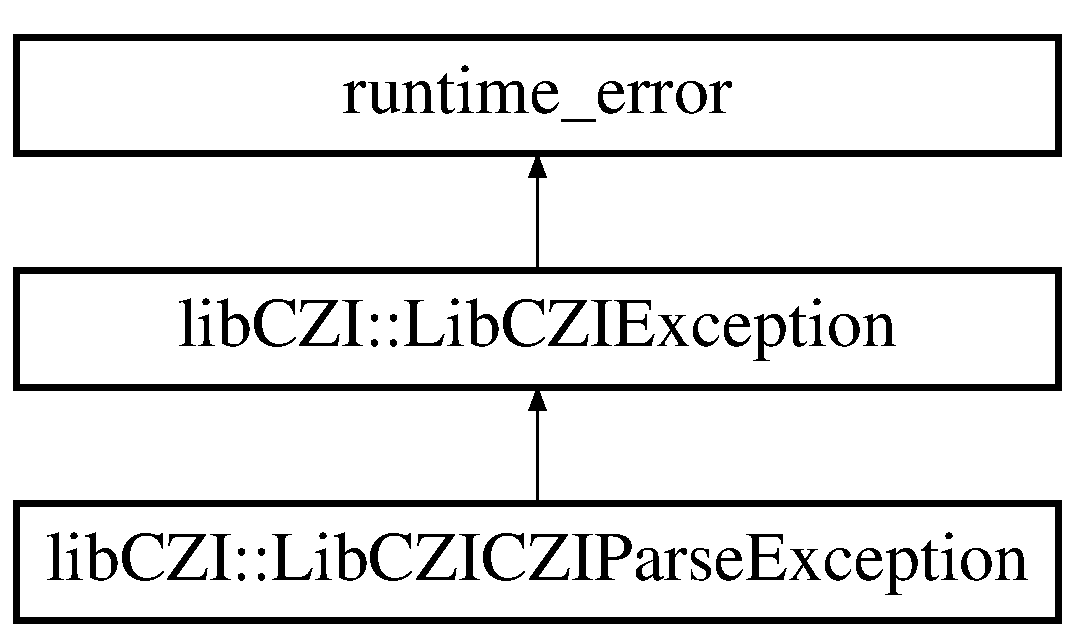
\includegraphics[height=3.000000cm]{structlib_c_z_i_1_1_lib_c_z_i_c_z_i_parse_exception}
\end{center}
\end{figure}
\subsection*{Public Types}
\begin{DoxyCompactItemize}
\item 
enum \hyperlink{structlib_c_z_i_1_1_lib_c_z_i_c_z_i_parse_exception_a32a6c8ab31a657e490e5c605c97efb40}{Error\+Code} \{ \hyperlink{structlib_c_z_i_1_1_lib_c_z_i_c_z_i_parse_exception_a32a6c8ab31a657e490e5c605c97efb40ab6e495eeaee7cdf1bac313472e4681ac}{Error\+Code\+::\+Not\+Enough\+Data}, 
\hyperlink{structlib_c_z_i_1_1_lib_c_z_i_c_z_i_parse_exception_a32a6c8ab31a657e490e5c605c97efb40a14ce06721aa54faf8e86a779a37ada3f}{Error\+Code\+::\+Corrupted\+Data}, 
\hyperlink{structlib_c_z_i_1_1_lib_c_z_i_c_z_i_parse_exception_a32a6c8ab31a657e490e5c605c97efb40a8462b58246e70e5c83e5b939a9332cb5}{Error\+Code\+::\+Internal\+Error}
 \}\begin{DoxyCompactList}\small\item\em Values that represent different error conditions. \end{DoxyCompactList}
\end{DoxyCompactItemize}
\subsection*{Public Member Functions}
\begin{DoxyCompactItemize}
\item 
\hyperlink{structlib_c_z_i_1_1_lib_c_z_i_c_z_i_parse_exception_aa5278cd2edeccba4b7cf8dd8f2ff58ef}{Lib\+C\+Z\+I\+C\+Z\+I\+Parse\+Exception} (const char $\ast$sz\+Err\+Msg, \hyperlink{structlib_c_z_i_1_1_lib_c_z_i_c_z_i_parse_exception_a32a6c8ab31a657e490e5c605c97efb40}{Error\+Code} code)
\item 
\hyperlink{structlib_c_z_i_1_1_lib_c_z_i_c_z_i_parse_exception_a32a6c8ab31a657e490e5c605c97efb40}{Error\+Code} \hyperlink{structlib_c_z_i_1_1_lib_c_z_i_c_z_i_parse_exception_af9f288e1c6b3eea97729bb47b7b61f27}{Get\+Error\+Code} () const
\end{DoxyCompactItemize}


\subsection{Detailed Description}
Exception for signaling errors parsing the C\+Z\+I-\/stream. 

\subsection{Member Enumeration Documentation}
\mbox{\Hypertarget{structlib_c_z_i_1_1_lib_c_z_i_c_z_i_parse_exception_a32a6c8ab31a657e490e5c605c97efb40}\label{structlib_c_z_i_1_1_lib_c_z_i_c_z_i_parse_exception_a32a6c8ab31a657e490e5c605c97efb40}} 
\index{lib\+C\+Z\+I\+::\+Lib\+C\+Z\+I\+C\+Z\+I\+Parse\+Exception@{lib\+C\+Z\+I\+::\+Lib\+C\+Z\+I\+C\+Z\+I\+Parse\+Exception}!Error\+Code@{Error\+Code}}
\index{Error\+Code@{Error\+Code}!lib\+C\+Z\+I\+::\+Lib\+C\+Z\+I\+C\+Z\+I\+Parse\+Exception@{lib\+C\+Z\+I\+::\+Lib\+C\+Z\+I\+C\+Z\+I\+Parse\+Exception}}
\subsubsection{\texorpdfstring{Error\+Code}{ErrorCode}}
{\footnotesize\ttfamily enum \hyperlink{structlib_c_z_i_1_1_lib_c_z_i_c_z_i_parse_exception_a32a6c8ab31a657e490e5c605c97efb40}{lib\+C\+Z\+I\+::\+Lib\+C\+Z\+I\+C\+Z\+I\+Parse\+Exception\+::\+Error\+Code}\hspace{0.3cm}{\ttfamily [strong]}}



Values that represent different error conditions. 

\begin{DoxyEnumFields}{Enumerator}
\raisebox{\heightof{T}}[0pt][0pt]{\index{Not\+Enough\+Data@{Not\+Enough\+Data}!lib\+C\+Z\+I\+::\+Lib\+C\+Z\+I\+C\+Z\+I\+Parse\+Exception@{lib\+C\+Z\+I\+::\+Lib\+C\+Z\+I\+C\+Z\+I\+Parse\+Exception}}\index{lib\+C\+Z\+I\+::\+Lib\+C\+Z\+I\+C\+Z\+I\+Parse\+Exception@{lib\+C\+Z\+I\+::\+Lib\+C\+Z\+I\+C\+Z\+I\+Parse\+Exception}!Not\+Enough\+Data@{Not\+Enough\+Data}}}\mbox{\Hypertarget{structlib_c_z_i_1_1_lib_c_z_i_c_z_i_parse_exception_a32a6c8ab31a657e490e5c605c97efb40ab6e495eeaee7cdf1bac313472e4681ac}\label{structlib_c_z_i_1_1_lib_c_z_i_c_z_i_parse_exception_a32a6c8ab31a657e490e5c605c97efb40ab6e495eeaee7cdf1bac313472e4681ac}} 
Not\+Enough\+Data&An enum constant representing that not the expected amount of data could be read. \\
\hline

\raisebox{\heightof{T}}[0pt][0pt]{\index{Corrupted\+Data@{Corrupted\+Data}!lib\+C\+Z\+I\+::\+Lib\+C\+Z\+I\+C\+Z\+I\+Parse\+Exception@{lib\+C\+Z\+I\+::\+Lib\+C\+Z\+I\+C\+Z\+I\+Parse\+Exception}}\index{lib\+C\+Z\+I\+::\+Lib\+C\+Z\+I\+C\+Z\+I\+Parse\+Exception@{lib\+C\+Z\+I\+::\+Lib\+C\+Z\+I\+C\+Z\+I\+Parse\+Exception}!Corrupted\+Data@{Corrupted\+Data}}}\mbox{\Hypertarget{structlib_c_z_i_1_1_lib_c_z_i_c_z_i_parse_exception_a32a6c8ab31a657e490e5c605c97efb40a14ce06721aa54faf8e86a779a37ada3f}\label{structlib_c_z_i_1_1_lib_c_z_i_c_z_i_parse_exception_a32a6c8ab31a657e490e5c605c97efb40a14ce06721aa54faf8e86a779a37ada3f}} 
Corrupted\+Data&An enum constant representing that the data was detected to be bogus. \\
\hline

\raisebox{\heightof{T}}[0pt][0pt]{\index{Internal\+Error@{Internal\+Error}!lib\+C\+Z\+I\+::\+Lib\+C\+Z\+I\+C\+Z\+I\+Parse\+Exception@{lib\+C\+Z\+I\+::\+Lib\+C\+Z\+I\+C\+Z\+I\+Parse\+Exception}}\index{lib\+C\+Z\+I\+::\+Lib\+C\+Z\+I\+C\+Z\+I\+Parse\+Exception@{lib\+C\+Z\+I\+::\+Lib\+C\+Z\+I\+C\+Z\+I\+Parse\+Exception}!Internal\+Error@{Internal\+Error}}}\mbox{\Hypertarget{structlib_c_z_i_1_1_lib_c_z_i_c_z_i_parse_exception_a32a6c8ab31a657e490e5c605c97efb40a8462b58246e70e5c83e5b939a9332cb5}\label{structlib_c_z_i_1_1_lib_c_z_i_c_z_i_parse_exception_a32a6c8ab31a657e490e5c605c97efb40a8462b58246e70e5c83e5b939a9332cb5}} 
Internal\+Error&An internal error was detected. \\
\hline

\end{DoxyEnumFields}


\subsection{Constructor \& Destructor Documentation}
\mbox{\Hypertarget{structlib_c_z_i_1_1_lib_c_z_i_c_z_i_parse_exception_aa5278cd2edeccba4b7cf8dd8f2ff58ef}\label{structlib_c_z_i_1_1_lib_c_z_i_c_z_i_parse_exception_aa5278cd2edeccba4b7cf8dd8f2ff58ef}} 
\index{lib\+C\+Z\+I\+::\+Lib\+C\+Z\+I\+C\+Z\+I\+Parse\+Exception@{lib\+C\+Z\+I\+::\+Lib\+C\+Z\+I\+C\+Z\+I\+Parse\+Exception}!Lib\+C\+Z\+I\+C\+Z\+I\+Parse\+Exception@{Lib\+C\+Z\+I\+C\+Z\+I\+Parse\+Exception}}
\index{Lib\+C\+Z\+I\+C\+Z\+I\+Parse\+Exception@{Lib\+C\+Z\+I\+C\+Z\+I\+Parse\+Exception}!lib\+C\+Z\+I\+::\+Lib\+C\+Z\+I\+C\+Z\+I\+Parse\+Exception@{lib\+C\+Z\+I\+::\+Lib\+C\+Z\+I\+C\+Z\+I\+Parse\+Exception}}
\subsubsection{\texorpdfstring{Lib\+C\+Z\+I\+C\+Z\+I\+Parse\+Exception()}{LibCZICZIParseException()}}
{\footnotesize\ttfamily lib\+C\+Z\+I\+::\+Lib\+C\+Z\+I\+C\+Z\+I\+Parse\+Exception\+::\+Lib\+C\+Z\+I\+C\+Z\+I\+Parse\+Exception (\begin{DoxyParamCaption}\item[{const char $\ast$}]{sz\+Err\+Msg,  }\item[{\hyperlink{structlib_c_z_i_1_1_lib_c_z_i_c_z_i_parse_exception_a32a6c8ab31a657e490e5c605c97efb40}{Error\+Code}}]{code }\end{DoxyParamCaption})\hspace{0.3cm}{\ttfamily [inline]}}

Constructor for the \hyperlink{structlib_c_z_i_1_1_lib_c_z_i_c_z_i_parse_exception}{Lib\+C\+Z\+I\+C\+Z\+I\+Parse\+Exception}. This type is used to signal that there was a parsing error. 
\begin{DoxyParams}{Parameters}
{\em sz\+Err\+Msg} & Message describing the error. \\
\hline
{\em code} & The error code. \\
\hline
\end{DoxyParams}


\subsection{Member Function Documentation}
\mbox{\Hypertarget{structlib_c_z_i_1_1_lib_c_z_i_c_z_i_parse_exception_af9f288e1c6b3eea97729bb47b7b61f27}\label{structlib_c_z_i_1_1_lib_c_z_i_c_z_i_parse_exception_af9f288e1c6b3eea97729bb47b7b61f27}} 
\index{lib\+C\+Z\+I\+::\+Lib\+C\+Z\+I\+C\+Z\+I\+Parse\+Exception@{lib\+C\+Z\+I\+::\+Lib\+C\+Z\+I\+C\+Z\+I\+Parse\+Exception}!Get\+Error\+Code@{Get\+Error\+Code}}
\index{Get\+Error\+Code@{Get\+Error\+Code}!lib\+C\+Z\+I\+::\+Lib\+C\+Z\+I\+C\+Z\+I\+Parse\+Exception@{lib\+C\+Z\+I\+::\+Lib\+C\+Z\+I\+C\+Z\+I\+Parse\+Exception}}
\subsubsection{\texorpdfstring{Get\+Error\+Code()}{GetErrorCode()}}
{\footnotesize\ttfamily \hyperlink{structlib_c_z_i_1_1_lib_c_z_i_c_z_i_parse_exception_a32a6c8ab31a657e490e5c605c97efb40}{Error\+Code} lib\+C\+Z\+I\+::\+Lib\+C\+Z\+I\+C\+Z\+I\+Parse\+Exception\+::\+Get\+Error\+Code (\begin{DoxyParamCaption}{ }\end{DoxyParamCaption}) const\hspace{0.3cm}{\ttfamily [inline]}}

Gets error code. \begin{DoxyReturn}{Returns}
The error code. 
\end{DoxyReturn}


The documentation for this struct was generated from the following file\+:\begin{DoxyCompactItemize}
\item 
lib\+C\+Z\+I/lib\+C\+Z\+I\+\_\+exceptions.\+h\end{DoxyCompactItemize}

\hypertarget{classlib_c_z_i_1_1_lib_c_z_i_exception}{}\section{lib\+C\+ZI\+:\+:Lib\+C\+Z\+I\+Exception Class Reference}
\label{classlib_c_z_i_1_1_lib_c_z_i_exception}\index{lib\+C\+Z\+I\+::\+Lib\+C\+Z\+I\+Exception@{lib\+C\+Z\+I\+::\+Lib\+C\+Z\+I\+Exception}}


Base class for all lib\+C\+Z\+I-\/specific exceptions.  




{\ttfamily \#include $<$lib\+C\+Z\+I\+\_\+exceptions.\+h$>$}

Inheritance diagram for lib\+C\+ZI\+:\+:Lib\+C\+Z\+I\+Exception\+:\begin{figure}[H]
\begin{center}
\leavevmode
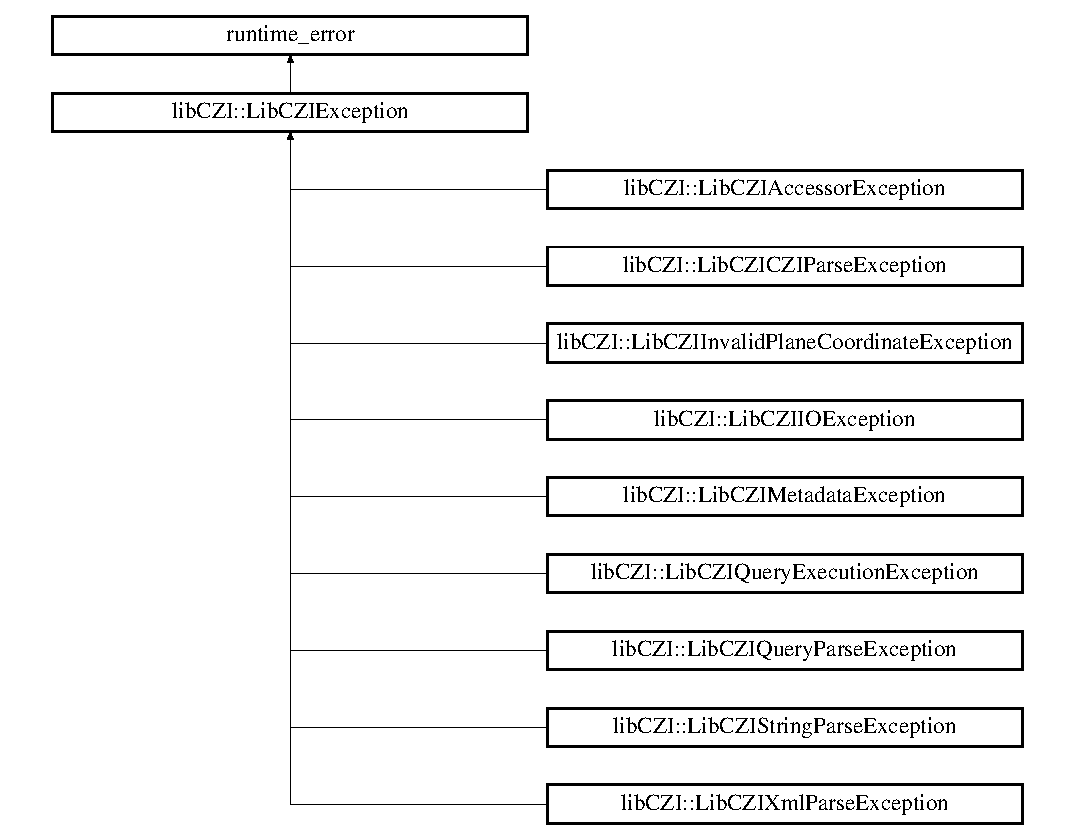
\includegraphics[height=10.845070cm]{classlib_c_z_i_1_1_lib_c_z_i_exception}
\end{center}
\end{figure}
\subsection*{Public Member Functions}
\begin{DoxyCompactItemize}
\item 
\hyperlink{classlib_c_z_i_1_1_lib_c_z_i_exception_ab6a09f2d1b399b1aa37f2ea75b80d6f8}{Lib\+C\+Z\+I\+Exception} (const char $\ast$sz\+Err\+Msg)
\end{DoxyCompactItemize}


\subsection{Detailed Description}
Base class for all lib\+C\+Z\+I-\/specific exceptions. 

\subsection{Constructor \& Destructor Documentation}
\mbox{\Hypertarget{classlib_c_z_i_1_1_lib_c_z_i_exception_ab6a09f2d1b399b1aa37f2ea75b80d6f8}\label{classlib_c_z_i_1_1_lib_c_z_i_exception_ab6a09f2d1b399b1aa37f2ea75b80d6f8}} 
\index{lib\+C\+Z\+I\+::\+Lib\+C\+Z\+I\+Exception@{lib\+C\+Z\+I\+::\+Lib\+C\+Z\+I\+Exception}!Lib\+C\+Z\+I\+Exception@{Lib\+C\+Z\+I\+Exception}}
\index{Lib\+C\+Z\+I\+Exception@{Lib\+C\+Z\+I\+Exception}!lib\+C\+Z\+I\+::\+Lib\+C\+Z\+I\+Exception@{lib\+C\+Z\+I\+::\+Lib\+C\+Z\+I\+Exception}}
\subsubsection{\texorpdfstring{Lib\+C\+Z\+I\+Exception()}{LibCZIException()}}
{\footnotesize\ttfamily lib\+C\+Z\+I\+::\+Lib\+C\+Z\+I\+Exception\+::\+Lib\+C\+Z\+I\+Exception (\begin{DoxyParamCaption}\item[{const char $\ast$}]{sz\+Err\+Msg }\end{DoxyParamCaption})\hspace{0.3cm}{\ttfamily [inline]}, {\ttfamily [explicit]}}

Constructor. 
\begin{DoxyParams}{Parameters}
{\em sz\+Err\+Msg} & Message describing the error. \\
\hline
\end{DoxyParams}


The documentation for this class was generated from the following file\+:\begin{DoxyCompactItemize}
\item 
lib\+C\+Z\+I/lib\+C\+Z\+I\+\_\+exceptions.\+h\end{DoxyCompactItemize}

\hypertarget{structlib_c_z_i_1_1_lib_c_z_i_invalid_plane_coordinate_exception}{}\section{lib\+C\+ZI\+:\+:Lib\+C\+Z\+I\+Invalid\+Plane\+Coordinate\+Exception Struct Reference}
\label{structlib_c_z_i_1_1_lib_c_z_i_invalid_plane_coordinate_exception}\index{lib\+C\+Z\+I\+::\+Lib\+C\+Z\+I\+Invalid\+Plane\+Coordinate\+Exception@{lib\+C\+Z\+I\+::\+Lib\+C\+Z\+I\+Invalid\+Plane\+Coordinate\+Exception}}


Exception for signaling an incorrect plane-\/coordinate object.  




{\ttfamily \#include $<$lib\+C\+Z\+I\+\_\+exceptions.\+h$>$}

Inheritance diagram for lib\+C\+ZI\+:\+:Lib\+C\+Z\+I\+Invalid\+Plane\+Coordinate\+Exception\+:\begin{figure}[H]
\begin{center}
\leavevmode
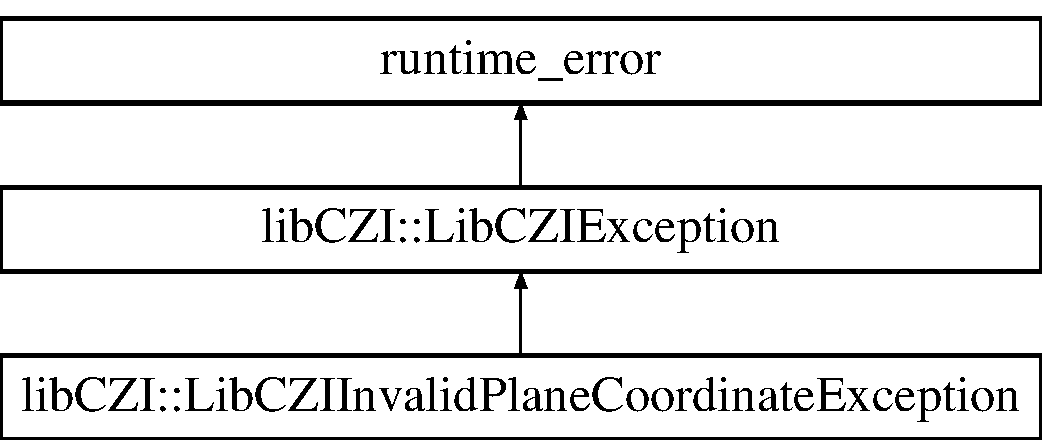
\includegraphics[height=3.000000cm]{structlib_c_z_i_1_1_lib_c_z_i_invalid_plane_coordinate_exception}
\end{center}
\end{figure}
\subsection*{Public Types}
\begin{DoxyCompactItemize}
\item 
enum \hyperlink{structlib_c_z_i_1_1_lib_c_z_i_invalid_plane_coordinate_exception_a2e22a8936930f8e8de4b874764407b60}{Error\+Code} \{ \hyperlink{structlib_c_z_i_1_1_lib_c_z_i_invalid_plane_coordinate_exception_a2e22a8936930f8e8de4b874764407b60a2387177c5eeb2b0165fb975f4b741c55}{Error\+Code\+::\+Surplus\+Dimension}, 
\hyperlink{structlib_c_z_i_1_1_lib_c_z_i_invalid_plane_coordinate_exception_a2e22a8936930f8e8de4b874764407b60a06a04b63fba5058c3dc36269ef6dfaaa}{Error\+Code\+::\+Missing\+Dimension}, 
\hyperlink{structlib_c_z_i_1_1_lib_c_z_i_invalid_plane_coordinate_exception_a2e22a8936930f8e8de4b874764407b60a32718a726c2956f702be80643045a4e1}{Error\+Code\+::\+Invalid\+Dimension}, 
\hyperlink{structlib_c_z_i_1_1_lib_c_z_i_invalid_plane_coordinate_exception_a2e22a8936930f8e8de4b874764407b60a4a35479ed0f04e5d5ea428427869570b}{Error\+Code\+::\+Coordinate\+Out\+Of\+Range}
 \}\begin{DoxyCompactList}\small\item\em Values that represent different error conditions. \end{DoxyCompactList}
\end{DoxyCompactItemize}
\subsection*{Public Member Functions}
\begin{DoxyCompactItemize}
\item 
\hyperlink{structlib_c_z_i_1_1_lib_c_z_i_invalid_plane_coordinate_exception_a574543a1bbfb24a9e01f3d3cb4666318}{Lib\+C\+Z\+I\+Invalid\+Plane\+Coordinate\+Exception} (const char $\ast$sz\+Err\+Msg, \hyperlink{structlib_c_z_i_1_1_lib_c_z_i_invalid_plane_coordinate_exception_a2e22a8936930f8e8de4b874764407b60}{Error\+Code} code)
\end{DoxyCompactItemize}


\subsection{Detailed Description}
Exception for signaling an incorrect plane-\/coordinate object. 

\subsection{Member Enumeration Documentation}
\mbox{\Hypertarget{structlib_c_z_i_1_1_lib_c_z_i_invalid_plane_coordinate_exception_a2e22a8936930f8e8de4b874764407b60}\label{structlib_c_z_i_1_1_lib_c_z_i_invalid_plane_coordinate_exception_a2e22a8936930f8e8de4b874764407b60}} 
\index{lib\+C\+Z\+I\+::\+Lib\+C\+Z\+I\+Invalid\+Plane\+Coordinate\+Exception@{lib\+C\+Z\+I\+::\+Lib\+C\+Z\+I\+Invalid\+Plane\+Coordinate\+Exception}!Error\+Code@{Error\+Code}}
\index{Error\+Code@{Error\+Code}!lib\+C\+Z\+I\+::\+Lib\+C\+Z\+I\+Invalid\+Plane\+Coordinate\+Exception@{lib\+C\+Z\+I\+::\+Lib\+C\+Z\+I\+Invalid\+Plane\+Coordinate\+Exception}}
\subsubsection{\texorpdfstring{Error\+Code}{ErrorCode}}
{\footnotesize\ttfamily enum \hyperlink{structlib_c_z_i_1_1_lib_c_z_i_invalid_plane_coordinate_exception_a2e22a8936930f8e8de4b874764407b60}{lib\+C\+Z\+I\+::\+Lib\+C\+Z\+I\+Invalid\+Plane\+Coordinate\+Exception\+::\+Error\+Code}\hspace{0.3cm}{\ttfamily [strong]}}



Values that represent different error conditions. 

\begin{DoxyEnumFields}{Enumerator}
\raisebox{\heightof{T}}[0pt][0pt]{\index{Surplus\+Dimension@{Surplus\+Dimension}!lib\+C\+Z\+I\+::\+Lib\+C\+Z\+I\+Invalid\+Plane\+Coordinate\+Exception@{lib\+C\+Z\+I\+::\+Lib\+C\+Z\+I\+Invalid\+Plane\+Coordinate\+Exception}}\index{lib\+C\+Z\+I\+::\+Lib\+C\+Z\+I\+Invalid\+Plane\+Coordinate\+Exception@{lib\+C\+Z\+I\+::\+Lib\+C\+Z\+I\+Invalid\+Plane\+Coordinate\+Exception}!Surplus\+Dimension@{Surplus\+Dimension}}}\mbox{\Hypertarget{structlib_c_z_i_1_1_lib_c_z_i_invalid_plane_coordinate_exception_a2e22a8936930f8e8de4b874764407b60a2387177c5eeb2b0165fb975f4b741c55}\label{structlib_c_z_i_1_1_lib_c_z_i_invalid_plane_coordinate_exception_a2e22a8936930f8e8de4b874764407b60a2387177c5eeb2b0165fb975f4b741c55}} 
Surplus\+Dimension&An enum constant representing a dimension was specified which is not found in the document. \\
\hline

\raisebox{\heightof{T}}[0pt][0pt]{\index{Missing\+Dimension@{Missing\+Dimension}!lib\+C\+Z\+I\+::\+Lib\+C\+Z\+I\+Invalid\+Plane\+Coordinate\+Exception@{lib\+C\+Z\+I\+::\+Lib\+C\+Z\+I\+Invalid\+Plane\+Coordinate\+Exception}}\index{lib\+C\+Z\+I\+::\+Lib\+C\+Z\+I\+Invalid\+Plane\+Coordinate\+Exception@{lib\+C\+Z\+I\+::\+Lib\+C\+Z\+I\+Invalid\+Plane\+Coordinate\+Exception}!Missing\+Dimension@{Missing\+Dimension}}}\mbox{\Hypertarget{structlib_c_z_i_1_1_lib_c_z_i_invalid_plane_coordinate_exception_a2e22a8936930f8e8de4b874764407b60a06a04b63fba5058c3dc36269ef6dfaaa}\label{structlib_c_z_i_1_1_lib_c_z_i_invalid_plane_coordinate_exception_a2e22a8936930f8e8de4b874764407b60a06a04b63fba5058c3dc36269ef6dfaaa}} 
Missing\+Dimension&An enum constant representing that the plane-\/coordinate did not contain a coordinate which is required to specify a plane. \\
\hline

\raisebox{\heightof{T}}[0pt][0pt]{\index{Invalid\+Dimension@{Invalid\+Dimension}!lib\+C\+Z\+I\+::\+Lib\+C\+Z\+I\+Invalid\+Plane\+Coordinate\+Exception@{lib\+C\+Z\+I\+::\+Lib\+C\+Z\+I\+Invalid\+Plane\+Coordinate\+Exception}}\index{lib\+C\+Z\+I\+::\+Lib\+C\+Z\+I\+Invalid\+Plane\+Coordinate\+Exception@{lib\+C\+Z\+I\+::\+Lib\+C\+Z\+I\+Invalid\+Plane\+Coordinate\+Exception}!Invalid\+Dimension@{Invalid\+Dimension}}}\mbox{\Hypertarget{structlib_c_z_i_1_1_lib_c_z_i_invalid_plane_coordinate_exception_a2e22a8936930f8e8de4b874764407b60a32718a726c2956f702be80643045a4e1}\label{structlib_c_z_i_1_1_lib_c_z_i_invalid_plane_coordinate_exception_a2e22a8936930f8e8de4b874764407b60a32718a726c2956f702be80643045a4e1}} 
Invalid\+Dimension&An enum constant representing that the plane-\/coordinate contained a dimension which is not used to specify a plane. \\
\hline

\raisebox{\heightof{T}}[0pt][0pt]{\index{Coordinate\+Out\+Of\+Range@{Coordinate\+Out\+Of\+Range}!lib\+C\+Z\+I\+::\+Lib\+C\+Z\+I\+Invalid\+Plane\+Coordinate\+Exception@{lib\+C\+Z\+I\+::\+Lib\+C\+Z\+I\+Invalid\+Plane\+Coordinate\+Exception}}\index{lib\+C\+Z\+I\+::\+Lib\+C\+Z\+I\+Invalid\+Plane\+Coordinate\+Exception@{lib\+C\+Z\+I\+::\+Lib\+C\+Z\+I\+Invalid\+Plane\+Coordinate\+Exception}!Coordinate\+Out\+Of\+Range@{Coordinate\+Out\+Of\+Range}}}\mbox{\Hypertarget{structlib_c_z_i_1_1_lib_c_z_i_invalid_plane_coordinate_exception_a2e22a8936930f8e8de4b874764407b60a4a35479ed0f04e5d5ea428427869570b}\label{structlib_c_z_i_1_1_lib_c_z_i_invalid_plane_coordinate_exception_a2e22a8936930f8e8de4b874764407b60a4a35479ed0f04e5d5ea428427869570b}} 
Coordinate\+Out\+Of\+Range&An enum constant representing that a coordinate was given which is out-\/of-\/range. \\
\hline

\end{DoxyEnumFields}


\subsection{Constructor \& Destructor Documentation}
\mbox{\Hypertarget{structlib_c_z_i_1_1_lib_c_z_i_invalid_plane_coordinate_exception_a574543a1bbfb24a9e01f3d3cb4666318}\label{structlib_c_z_i_1_1_lib_c_z_i_invalid_plane_coordinate_exception_a574543a1bbfb24a9e01f3d3cb4666318}} 
\index{lib\+C\+Z\+I\+::\+Lib\+C\+Z\+I\+Invalid\+Plane\+Coordinate\+Exception@{lib\+C\+Z\+I\+::\+Lib\+C\+Z\+I\+Invalid\+Plane\+Coordinate\+Exception}!Lib\+C\+Z\+I\+Invalid\+Plane\+Coordinate\+Exception@{Lib\+C\+Z\+I\+Invalid\+Plane\+Coordinate\+Exception}}
\index{Lib\+C\+Z\+I\+Invalid\+Plane\+Coordinate\+Exception@{Lib\+C\+Z\+I\+Invalid\+Plane\+Coordinate\+Exception}!lib\+C\+Z\+I\+::\+Lib\+C\+Z\+I\+Invalid\+Plane\+Coordinate\+Exception@{lib\+C\+Z\+I\+::\+Lib\+C\+Z\+I\+Invalid\+Plane\+Coordinate\+Exception}}
\subsubsection{\texorpdfstring{Lib\+C\+Z\+I\+Invalid\+Plane\+Coordinate\+Exception()}{LibCZIInvalidPlaneCoordinateException()}}
{\footnotesize\ttfamily lib\+C\+Z\+I\+::\+Lib\+C\+Z\+I\+Invalid\+Plane\+Coordinate\+Exception\+::\+Lib\+C\+Z\+I\+Invalid\+Plane\+Coordinate\+Exception (\begin{DoxyParamCaption}\item[{const char $\ast$}]{sz\+Err\+Msg,  }\item[{\hyperlink{structlib_c_z_i_1_1_lib_c_z_i_invalid_plane_coordinate_exception_a2e22a8936930f8e8de4b874764407b60}{Error\+Code}}]{code }\end{DoxyParamCaption})\hspace{0.3cm}{\ttfamily [inline]}}

Constructor for the \hyperlink{structlib_c_z_i_1_1_lib_c_z_i_invalid_plane_coordinate_exception}{Lib\+C\+Z\+I\+Invalid\+Plane\+Coordinate\+Exception}. This type is used to signal that a plane-\/coordinate was determined to be invalid. 
\begin{DoxyParams}{Parameters}
{\em sz\+Err\+Msg} & Message describing the error. \\
\hline
{\em code} & The error code. \\
\hline
\end{DoxyParams}


The documentation for this struct was generated from the following file\+:\begin{DoxyCompactItemize}
\item 
lib\+C\+Z\+I/lib\+C\+Z\+I\+\_\+exceptions.\+h\end{DoxyCompactItemize}

\hypertarget{classlib_c_z_i_1_1_lib_c_z_i_i_o_exception}{}\section{lib\+C\+ZI\+:\+:Lib\+C\+Z\+I\+I\+O\+Exception Class Reference}
\label{classlib_c_z_i_1_1_lib_c_z_i_i_o_exception}\index{lib\+C\+Z\+I\+::\+Lib\+C\+Z\+I\+I\+O\+Exception@{lib\+C\+Z\+I\+::\+Lib\+C\+Z\+I\+I\+O\+Exception}}


{\ttfamily \#include $<$lib\+C\+Z\+I\+\_\+exceptions.\+h$>$}

Inheritance diagram for lib\+C\+ZI\+:\+:Lib\+C\+Z\+I\+I\+O\+Exception\+:\begin{figure}[H]
\begin{center}
\leavevmode
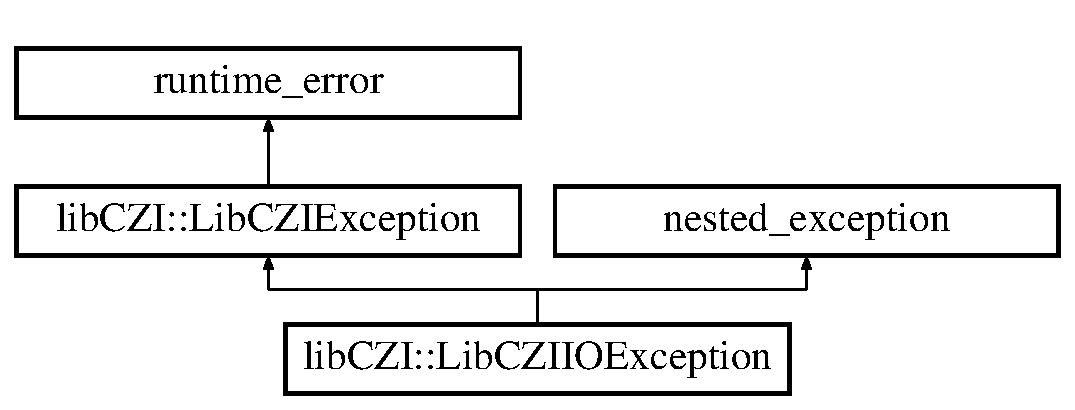
\includegraphics[height=3.000000cm]{classlib_c_z_i_1_1_lib_c_z_i_i_o_exception}
\end{center}
\end{figure}
\subsection*{Public Member Functions}
\begin{DoxyCompactItemize}
\item 
\hyperlink{classlib_c_z_i_1_1_lib_c_z_i_i_o_exception_aa8912797c22c48afee6e24bdb1e03008}{Lib\+C\+Z\+I\+I\+O\+Exception} (const char $\ast$sz\+Err\+Msg, std\+::uint64\+\_\+t offset, std\+::uint64\+\_\+t size)
\item 
std\+::uint64\+\_\+t \hyperlink{classlib_c_z_i_1_1_lib_c_z_i_i_o_exception_a74781fd4547321f2e81e04028f385fd8}{Get\+Offset} () const
\item 
std\+::uint64\+\_\+t \hyperlink{classlib_c_z_i_1_1_lib_c_z_i_i_o_exception_affd1d9993181dbbed726234b01c1eca7}{Get\+Size} () const
\end{DoxyCompactItemize}


\subsection{Detailed Description}
Exception for signaling an I/O error. If the problem originates from the (external) stream-\/object, then the original exception is enclosed here as a nested exception. In order to access the nested exception, use something like this\+: 
\begin{DoxyCode}
\textcolor{keywordflow}{try}
    \{
        spReader->Open(stream);
    \}
    \textcolor{keywordflow}{catch} (\hyperlink{classlib_c_z_i_1_1_lib_c_z_i_i_o_exception_aa8912797c22c48afee6e24bdb1e03008}{LibCZIIOException}& excp)
    \{
        \textcolor{keywordflow}{try}
        \{
            excp.rethrow\_nested();
        \}
        \textcolor{keywordflow}{catch} (std::ios\_base::failure& innerExcp) \textcolor{comment}{// assuming that is the exception you }
        \{                                         \textcolor{comment}{// expect to be thrown from the stream-object}
         ....
        \}
    \}
\end{DoxyCode}
 

\subsection{Constructor \& Destructor Documentation}
\mbox{\Hypertarget{classlib_c_z_i_1_1_lib_c_z_i_i_o_exception_aa8912797c22c48afee6e24bdb1e03008}\label{classlib_c_z_i_1_1_lib_c_z_i_i_o_exception_aa8912797c22c48afee6e24bdb1e03008}} 
\index{lib\+C\+Z\+I\+::\+Lib\+C\+Z\+I\+I\+O\+Exception@{lib\+C\+Z\+I\+::\+Lib\+C\+Z\+I\+I\+O\+Exception}!Lib\+C\+Z\+I\+I\+O\+Exception@{Lib\+C\+Z\+I\+I\+O\+Exception}}
\index{Lib\+C\+Z\+I\+I\+O\+Exception@{Lib\+C\+Z\+I\+I\+O\+Exception}!lib\+C\+Z\+I\+::\+Lib\+C\+Z\+I\+I\+O\+Exception@{lib\+C\+Z\+I\+::\+Lib\+C\+Z\+I\+I\+O\+Exception}}
\subsubsection{\texorpdfstring{Lib\+C\+Z\+I\+I\+O\+Exception()}{LibCZIIOException()}}
{\footnotesize\ttfamily lib\+C\+Z\+I\+::\+Lib\+C\+Z\+I\+I\+O\+Exception\+::\+Lib\+C\+Z\+I\+I\+O\+Exception (\begin{DoxyParamCaption}\item[{const char $\ast$}]{sz\+Err\+Msg,  }\item[{std\+::uint64\+\_\+t}]{offset,  }\item[{std\+::uint64\+\_\+t}]{size }\end{DoxyParamCaption})\hspace{0.3cm}{\ttfamily [inline]}}

Constructor for the \hyperlink{classlib_c_z_i_1_1_lib_c_z_i_i_o_exception}{Lib\+C\+Z\+I\+I\+O\+Exception}. This type is used to signal an I/\+O-\/error from the underlying stream.


\begin{DoxyParams}{Parameters}
{\em sz\+Err\+Msg} & Message describing the error. \\
\hline
{\em offset} & The offset (into the stream) at which the I/\+O-\/error occured. \\
\hline
{\em size} & The size of data we have attempted to read (when the I/\+O-\/error occured). \\
\hline
\end{DoxyParams}


\subsection{Member Function Documentation}
\mbox{\Hypertarget{classlib_c_z_i_1_1_lib_c_z_i_i_o_exception_a74781fd4547321f2e81e04028f385fd8}\label{classlib_c_z_i_1_1_lib_c_z_i_i_o_exception_a74781fd4547321f2e81e04028f385fd8}} 
\index{lib\+C\+Z\+I\+::\+Lib\+C\+Z\+I\+I\+O\+Exception@{lib\+C\+Z\+I\+::\+Lib\+C\+Z\+I\+I\+O\+Exception}!Get\+Offset@{Get\+Offset}}
\index{Get\+Offset@{Get\+Offset}!lib\+C\+Z\+I\+::\+Lib\+C\+Z\+I\+I\+O\+Exception@{lib\+C\+Z\+I\+::\+Lib\+C\+Z\+I\+I\+O\+Exception}}
\subsubsection{\texorpdfstring{Get\+Offset()}{GetOffset()}}
{\footnotesize\ttfamily std\+::uint64\+\_\+t lib\+C\+Z\+I\+::\+Lib\+C\+Z\+I\+I\+O\+Exception\+::\+Get\+Offset (\begin{DoxyParamCaption}{ }\end{DoxyParamCaption}) const\hspace{0.3cm}{\ttfamily [inline]}}

Gets the offset (in bytes) into the stream at which the I/\+O-\/error occured.

\begin{DoxyReturn}{Returns}
The offset (in bytes). 
\end{DoxyReturn}
\mbox{\Hypertarget{classlib_c_z_i_1_1_lib_c_z_i_i_o_exception_affd1d9993181dbbed726234b01c1eca7}\label{classlib_c_z_i_1_1_lib_c_z_i_i_o_exception_affd1d9993181dbbed726234b01c1eca7}} 
\index{lib\+C\+Z\+I\+::\+Lib\+C\+Z\+I\+I\+O\+Exception@{lib\+C\+Z\+I\+::\+Lib\+C\+Z\+I\+I\+O\+Exception}!Get\+Size@{Get\+Size}}
\index{Get\+Size@{Get\+Size}!lib\+C\+Z\+I\+::\+Lib\+C\+Z\+I\+I\+O\+Exception@{lib\+C\+Z\+I\+::\+Lib\+C\+Z\+I\+I\+O\+Exception}}
\subsubsection{\texorpdfstring{Get\+Size()}{GetSize()}}
{\footnotesize\ttfamily std\+::uint64\+\_\+t lib\+C\+Z\+I\+::\+Lib\+C\+Z\+I\+I\+O\+Exception\+::\+Get\+Size (\begin{DoxyParamCaption}{ }\end{DoxyParamCaption}) const\hspace{0.3cm}{\ttfamily [inline]}}

Gets the size of data (in bytes) we attempted to read when the I/\+O-\/error occured.

\begin{DoxyReturn}{Returns}
The size (in bytes). 
\end{DoxyReturn}


The documentation for this class was generated from the following file\+:\begin{DoxyCompactItemize}
\item 
lib\+C\+Z\+I/lib\+C\+Z\+I\+\_\+exceptions.\+h\end{DoxyCompactItemize}

\hypertarget{classlib_c_z_i_1_1_lib_c_z_i_metadata_exception}{}\section{lib\+C\+ZI\+:\+:Lib\+C\+Z\+I\+Metadata\+Exception Class Reference}
\label{classlib_c_z_i_1_1_lib_c_z_i_metadata_exception}\index{lib\+C\+Z\+I\+::\+Lib\+C\+Z\+I\+Metadata\+Exception@{lib\+C\+Z\+I\+::\+Lib\+C\+Z\+I\+Metadata\+Exception}}


Exception for signaling errors when accessing the X\+M\+L-\/metadata.  




{\ttfamily \#include $<$lib\+C\+Z\+I\+\_\+exceptions.\+h$>$}

Inheritance diagram for lib\+C\+ZI\+:\+:Lib\+C\+Z\+I\+Metadata\+Exception\+:\begin{figure}[H]
\begin{center}
\leavevmode
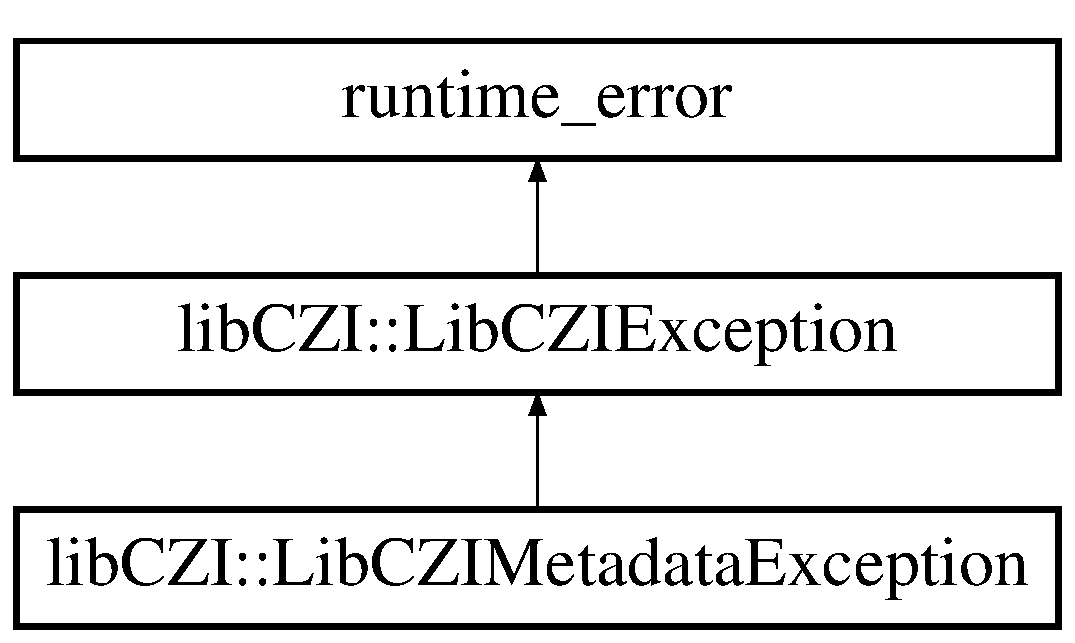
\includegraphics[height=3.000000cm]{classlib_c_z_i_1_1_lib_c_z_i_metadata_exception}
\end{center}
\end{figure}
\subsection*{Public Types}
\begin{DoxyCompactItemize}
\item 
enum \hyperlink{classlib_c_z_i_1_1_lib_c_z_i_metadata_exception_a60fe07e00ad32f331a85aafedec72242}{Error\+Type} \{ \hyperlink{classlib_c_z_i_1_1_lib_c_z_i_metadata_exception_a60fe07e00ad32f331a85aafedec72242a5d0744802b24f44a161d350c25d76c7b}{Error\+Type\+::\+Invalid\+Path}
 \}\begin{DoxyCompactList}\small\item\em Values that represent different error conditions. \end{DoxyCompactList}
\end{DoxyCompactItemize}
\subsection*{Public Member Functions}
\begin{DoxyCompactItemize}
\item 
\hyperlink{classlib_c_z_i_1_1_lib_c_z_i_metadata_exception_aa424dbc90e0fd24bc94da6a1021d3606}{Lib\+C\+Z\+I\+Metadata\+Exception} (const char $\ast$sz\+Err\+Msg, \hyperlink{classlib_c_z_i_1_1_lib_c_z_i_metadata_exception_a60fe07e00ad32f331a85aafedec72242}{Error\+Type} code)
\item 
\hyperlink{classlib_c_z_i_1_1_lib_c_z_i_metadata_exception_a60fe07e00ad32f331a85aafedec72242}{Error\+Type} \hyperlink{classlib_c_z_i_1_1_lib_c_z_i_metadata_exception_a0ea32f2d1a6b8a868617209a2984b167}{Get\+Error\+Type} () const
\end{DoxyCompactItemize}


\subsection{Detailed Description}
Exception for signaling errors when accessing the X\+M\+L-\/metadata. 

\subsection{Member Enumeration Documentation}
\mbox{\Hypertarget{classlib_c_z_i_1_1_lib_c_z_i_metadata_exception_a60fe07e00ad32f331a85aafedec72242}\label{classlib_c_z_i_1_1_lib_c_z_i_metadata_exception_a60fe07e00ad32f331a85aafedec72242}} 
\index{lib\+C\+Z\+I\+::\+Lib\+C\+Z\+I\+Metadata\+Exception@{lib\+C\+Z\+I\+::\+Lib\+C\+Z\+I\+Metadata\+Exception}!Error\+Type@{Error\+Type}}
\index{Error\+Type@{Error\+Type}!lib\+C\+Z\+I\+::\+Lib\+C\+Z\+I\+Metadata\+Exception@{lib\+C\+Z\+I\+::\+Lib\+C\+Z\+I\+Metadata\+Exception}}
\subsubsection{\texorpdfstring{Error\+Type}{ErrorType}}
{\footnotesize\ttfamily enum \hyperlink{classlib_c_z_i_1_1_lib_c_z_i_metadata_exception_a60fe07e00ad32f331a85aafedec72242}{lib\+C\+Z\+I\+::\+Lib\+C\+Z\+I\+Metadata\+Exception\+::\+Error\+Type}\hspace{0.3cm}{\ttfamily [strong]}}



Values that represent different error conditions. 

\begin{DoxyEnumFields}{Enumerator}
\raisebox{\heightof{T}}[0pt][0pt]{\index{Invalid\+Path@{Invalid\+Path}!lib\+C\+Z\+I\+::\+Lib\+C\+Z\+I\+Metadata\+Exception@{lib\+C\+Z\+I\+::\+Lib\+C\+Z\+I\+Metadata\+Exception}}\index{lib\+C\+Z\+I\+::\+Lib\+C\+Z\+I\+Metadata\+Exception@{lib\+C\+Z\+I\+::\+Lib\+C\+Z\+I\+Metadata\+Exception}!Invalid\+Path@{Invalid\+Path}}}\mbox{\Hypertarget{classlib_c_z_i_1_1_lib_c_z_i_metadata_exception_a60fe07e00ad32f331a85aafedec72242a5d0744802b24f44a161d350c25d76c7b}\label{classlib_c_z_i_1_1_lib_c_z_i_metadata_exception_a60fe07e00ad32f331a85aafedec72242a5d0744802b24f44a161d350c25d76c7b}} 
Invalid\+Path&the path specified in a call to \hyperlink{classlib_c_z_i_1_1_i_xml_node_read_a4e14de646b5624daf11b16ba42094c74}{I\+Xml\+Node\+Read\+::\+Get\+Child\+Node\+Readonly} was invalid \\
\hline

\end{DoxyEnumFields}


\subsection{Constructor \& Destructor Documentation}
\mbox{\Hypertarget{classlib_c_z_i_1_1_lib_c_z_i_metadata_exception_aa424dbc90e0fd24bc94da6a1021d3606}\label{classlib_c_z_i_1_1_lib_c_z_i_metadata_exception_aa424dbc90e0fd24bc94da6a1021d3606}} 
\index{lib\+C\+Z\+I\+::\+Lib\+C\+Z\+I\+Metadata\+Exception@{lib\+C\+Z\+I\+::\+Lib\+C\+Z\+I\+Metadata\+Exception}!Lib\+C\+Z\+I\+Metadata\+Exception@{Lib\+C\+Z\+I\+Metadata\+Exception}}
\index{Lib\+C\+Z\+I\+Metadata\+Exception@{Lib\+C\+Z\+I\+Metadata\+Exception}!lib\+C\+Z\+I\+::\+Lib\+C\+Z\+I\+Metadata\+Exception@{lib\+C\+Z\+I\+::\+Lib\+C\+Z\+I\+Metadata\+Exception}}
\subsubsection{\texorpdfstring{Lib\+C\+Z\+I\+Metadata\+Exception()}{LibCZIMetadataException()}}
{\footnotesize\ttfamily lib\+C\+Z\+I\+::\+Lib\+C\+Z\+I\+Metadata\+Exception\+::\+Lib\+C\+Z\+I\+Metadata\+Exception (\begin{DoxyParamCaption}\item[{const char $\ast$}]{sz\+Err\+Msg,  }\item[{\hyperlink{classlib_c_z_i_1_1_lib_c_z_i_metadata_exception_a60fe07e00ad32f331a85aafedec72242}{Error\+Type}}]{code }\end{DoxyParamCaption})\hspace{0.3cm}{\ttfamily [inline]}}

Constructor for the Lib\+C\+Z\+I\+Metadata\+Builder\+Exception. This type is used to signal errors when using the Czi-\/metadata-\/builder-\/object. 
\begin{DoxyParams}{Parameters}
{\em sz\+Err\+Msg} & Message describing the error. \\
\hline
{\em code} & The error code. \\
\hline
\end{DoxyParams}


\subsection{Member Function Documentation}
\mbox{\Hypertarget{classlib_c_z_i_1_1_lib_c_z_i_metadata_exception_a0ea32f2d1a6b8a868617209a2984b167}\label{classlib_c_z_i_1_1_lib_c_z_i_metadata_exception_a0ea32f2d1a6b8a868617209a2984b167}} 
\index{lib\+C\+Z\+I\+::\+Lib\+C\+Z\+I\+Metadata\+Exception@{lib\+C\+Z\+I\+::\+Lib\+C\+Z\+I\+Metadata\+Exception}!Get\+Error\+Type@{Get\+Error\+Type}}
\index{Get\+Error\+Type@{Get\+Error\+Type}!lib\+C\+Z\+I\+::\+Lib\+C\+Z\+I\+Metadata\+Exception@{lib\+C\+Z\+I\+::\+Lib\+C\+Z\+I\+Metadata\+Exception}}
\subsubsection{\texorpdfstring{Get\+Error\+Type()}{GetErrorType()}}
{\footnotesize\ttfamily \hyperlink{classlib_c_z_i_1_1_lib_c_z_i_metadata_exception_a60fe07e00ad32f331a85aafedec72242}{Error\+Type} lib\+C\+Z\+I\+::\+Lib\+C\+Z\+I\+Metadata\+Exception\+::\+Get\+Error\+Type (\begin{DoxyParamCaption}{ }\end{DoxyParamCaption}) const\hspace{0.3cm}{\ttfamily [inline]}}

Gets error code. \begin{DoxyReturn}{Returns}
The error code. 
\end{DoxyReturn}


The documentation for this class was generated from the following file\+:\begin{DoxyCompactItemize}
\item 
lib\+C\+Z\+I/lib\+C\+Z\+I\+\_\+exceptions.\+h\end{DoxyCompactItemize}

\hypertarget{classlib_c_z_i_1_1_lib_c_z_i_query_execution_exception}{}\section{lib\+C\+ZI\+:\+:Lib\+C\+Z\+I\+Query\+Execution\+Exception Class Reference}
\label{classlib_c_z_i_1_1_lib_c_z_i_query_execution_exception}\index{lib\+C\+Z\+I\+::\+Lib\+C\+Z\+I\+Query\+Execution\+Exception@{lib\+C\+Z\+I\+::\+Lib\+C\+Z\+I\+Query\+Execution\+Exception}}


Exception for signaling errors when evaluating a query.  




{\ttfamily \#include $<$lib\+C\+Z\+I\+\_\+exceptions.\+h$>$}

Inheritance diagram for lib\+C\+ZI\+:\+:Lib\+C\+Z\+I\+Query\+Execution\+Exception\+:\begin{figure}[H]
\begin{center}
\leavevmode
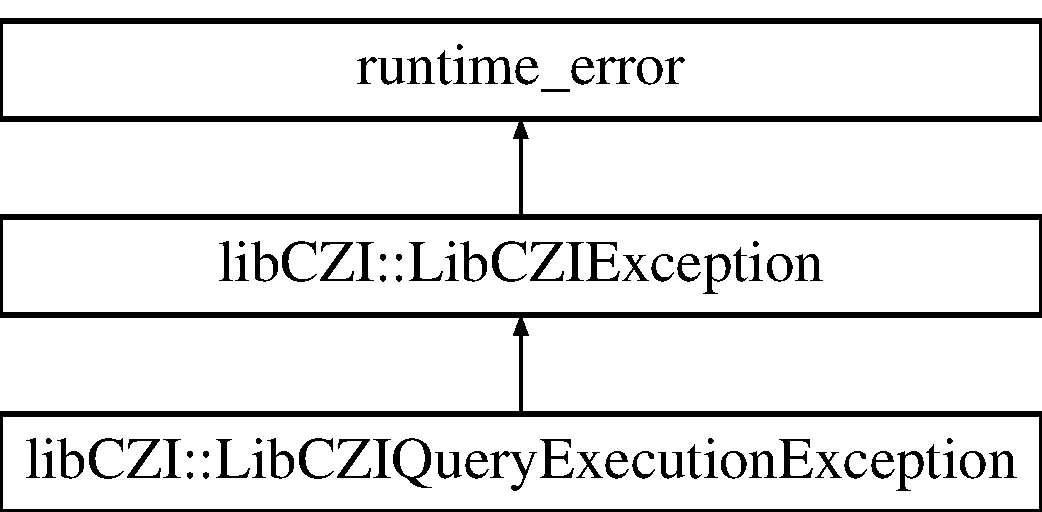
\includegraphics[height=3.000000cm]{classlib_c_z_i_1_1_lib_c_z_i_query_execution_exception}
\end{center}
\end{figure}
\subsection*{Public Types}
\begin{DoxyCompactItemize}
\item 
\mbox{\Hypertarget{classlib_c_z_i_1_1_lib_c_z_i_query_execution_exception_a7420fe8895248c44d16cf34f23f0c6a2}\label{classlib_c_z_i_1_1_lib_c_z_i_query_execution_exception_a7420fe8895248c44d16cf34f23f0c6a2}} 
enum \hyperlink{classlib_c_z_i_1_1_lib_c_z_i_query_execution_exception_a7420fe8895248c44d16cf34f23f0c6a2}{Error\+Type} \{ {\bfseries Non\+Existent\+Dimension}, 
{\bfseries Internal\+Error}
 \}\begin{DoxyCompactList}\small\item\em Values that represent different error conditions. \end{DoxyCompactList}
\end{DoxyCompactItemize}
\subsection*{Public Member Functions}
\begin{DoxyCompactItemize}
\item 
\hyperlink{classlib_c_z_i_1_1_lib_c_z_i_query_execution_exception_a9d19dc34e051c17ae74906794b72107f}{Lib\+C\+Z\+I\+Query\+Execution\+Exception} (const char $\ast$sz\+Err\+Msg, \hyperlink{classlib_c_z_i_1_1_lib_c_z_i_query_execution_exception_a7420fe8895248c44d16cf34f23f0c6a2}{Error\+Type} error\+Type)
\item 
\hyperlink{classlib_c_z_i_1_1_lib_c_z_i_query_execution_exception_a15b965e779ae464f4d2b5c1e7948db9a}{Lib\+C\+Z\+I\+Query\+Execution\+Exception} (const std\+::string \&err\+Msg, \hyperlink{classlib_c_z_i_1_1_lib_c_z_i_query_execution_exception_a7420fe8895248c44d16cf34f23f0c6a2}{Error\+Type} error\+Type)
\item 
\hyperlink{classlib_c_z_i_1_1_lib_c_z_i_query_execution_exception_a7420fe8895248c44d16cf34f23f0c6a2}{Error\+Type} \hyperlink{classlib_c_z_i_1_1_lib_c_z_i_query_execution_exception_a6ac7e255c61dae5fc104f0ae54d10513}{Get\+Error\+Type} () const
\end{DoxyCompactItemize}


\subsection{Detailed Description}
Exception for signaling errors when evaluating a query. 

\subsection{Constructor \& Destructor Documentation}
\mbox{\Hypertarget{classlib_c_z_i_1_1_lib_c_z_i_query_execution_exception_a9d19dc34e051c17ae74906794b72107f}\label{classlib_c_z_i_1_1_lib_c_z_i_query_execution_exception_a9d19dc34e051c17ae74906794b72107f}} 
\index{lib\+C\+Z\+I\+::\+Lib\+C\+Z\+I\+Query\+Execution\+Exception@{lib\+C\+Z\+I\+::\+Lib\+C\+Z\+I\+Query\+Execution\+Exception}!Lib\+C\+Z\+I\+Query\+Execution\+Exception@{Lib\+C\+Z\+I\+Query\+Execution\+Exception}}
\index{Lib\+C\+Z\+I\+Query\+Execution\+Exception@{Lib\+C\+Z\+I\+Query\+Execution\+Exception}!lib\+C\+Z\+I\+::\+Lib\+C\+Z\+I\+Query\+Execution\+Exception@{lib\+C\+Z\+I\+::\+Lib\+C\+Z\+I\+Query\+Execution\+Exception}}
\subsubsection{\texorpdfstring{Lib\+C\+Z\+I\+Query\+Execution\+Exception()}{LibCZIQueryExecutionException()}\hspace{0.1cm}{\footnotesize\ttfamily [1/2]}}
{\footnotesize\ttfamily lib\+C\+Z\+I\+::\+Lib\+C\+Z\+I\+Query\+Execution\+Exception\+::\+Lib\+C\+Z\+I\+Query\+Execution\+Exception (\begin{DoxyParamCaption}\item[{const char $\ast$}]{sz\+Err\+Msg,  }\item[{\hyperlink{classlib_c_z_i_1_1_lib_c_z_i_query_execution_exception_a7420fe8895248c44d16cf34f23f0c6a2}{Error\+Type}}]{error\+Type }\end{DoxyParamCaption})\hspace{0.3cm}{\ttfamily [inline]}, {\ttfamily [explicit]}}

Constructor for the Lib\+C\+Z\+I\+Query\+Execution\+Exception-\/exception. This exception is used to signal errors when evaluating a query. 
\begin{DoxyParams}{Parameters}
{\em sz\+Err\+Msg} & Message describing the error. \\
\hline
{\em error\+Type} & Type of the error. \\
\hline
\end{DoxyParams}
\mbox{\Hypertarget{classlib_c_z_i_1_1_lib_c_z_i_query_execution_exception_a15b965e779ae464f4d2b5c1e7948db9a}\label{classlib_c_z_i_1_1_lib_c_z_i_query_execution_exception_a15b965e779ae464f4d2b5c1e7948db9a}} 
\index{lib\+C\+Z\+I\+::\+Lib\+C\+Z\+I\+Query\+Execution\+Exception@{lib\+C\+Z\+I\+::\+Lib\+C\+Z\+I\+Query\+Execution\+Exception}!Lib\+C\+Z\+I\+Query\+Execution\+Exception@{Lib\+C\+Z\+I\+Query\+Execution\+Exception}}
\index{Lib\+C\+Z\+I\+Query\+Execution\+Exception@{Lib\+C\+Z\+I\+Query\+Execution\+Exception}!lib\+C\+Z\+I\+::\+Lib\+C\+Z\+I\+Query\+Execution\+Exception@{lib\+C\+Z\+I\+::\+Lib\+C\+Z\+I\+Query\+Execution\+Exception}}
\subsubsection{\texorpdfstring{Lib\+C\+Z\+I\+Query\+Execution\+Exception()}{LibCZIQueryExecutionException()}\hspace{0.1cm}{\footnotesize\ttfamily [2/2]}}
{\footnotesize\ttfamily lib\+C\+Z\+I\+::\+Lib\+C\+Z\+I\+Query\+Execution\+Exception\+::\+Lib\+C\+Z\+I\+Query\+Execution\+Exception (\begin{DoxyParamCaption}\item[{const std\+::string \&}]{err\+Msg,  }\item[{\hyperlink{classlib_c_z_i_1_1_lib_c_z_i_query_execution_exception_a7420fe8895248c44d16cf34f23f0c6a2}{Error\+Type}}]{error\+Type }\end{DoxyParamCaption})\hspace{0.3cm}{\ttfamily [inline]}, {\ttfamily [explicit]}}

Constructor for the Lib\+C\+Z\+I\+Query\+Execution\+Exception-\/exception. This exception is used to signal errors when evaluating a query. 
\begin{DoxyParams}{Parameters}
{\em err\+Msg} & Message describing the error. \\
\hline
{\em error\+Type} & Type of the error. \\
\hline
\end{DoxyParams}


\subsection{Member Function Documentation}
\mbox{\Hypertarget{classlib_c_z_i_1_1_lib_c_z_i_query_execution_exception_a6ac7e255c61dae5fc104f0ae54d10513}\label{classlib_c_z_i_1_1_lib_c_z_i_query_execution_exception_a6ac7e255c61dae5fc104f0ae54d10513}} 
\index{lib\+C\+Z\+I\+::\+Lib\+C\+Z\+I\+Query\+Execution\+Exception@{lib\+C\+Z\+I\+::\+Lib\+C\+Z\+I\+Query\+Execution\+Exception}!Get\+Error\+Type@{Get\+Error\+Type}}
\index{Get\+Error\+Type@{Get\+Error\+Type}!lib\+C\+Z\+I\+::\+Lib\+C\+Z\+I\+Query\+Execution\+Exception@{lib\+C\+Z\+I\+::\+Lib\+C\+Z\+I\+Query\+Execution\+Exception}}
\subsubsection{\texorpdfstring{Get\+Error\+Type()}{GetErrorType()}}
{\footnotesize\ttfamily \hyperlink{classlib_c_z_i_1_1_lib_c_z_i_query_execution_exception_a7420fe8895248c44d16cf34f23f0c6a2}{Error\+Type} lib\+C\+Z\+I\+::\+Lib\+C\+Z\+I\+Query\+Execution\+Exception\+::\+Get\+Error\+Type (\begin{DoxyParamCaption}{ }\end{DoxyParamCaption}) const\hspace{0.3cm}{\ttfamily [inline]}}

Gets error type \begin{DoxyReturn}{Returns}
The error type. 
\end{DoxyReturn}


The documentation for this class was generated from the following file\+:\begin{DoxyCompactItemize}
\item 
lib\+C\+Z\+I/lib\+C\+Z\+I\+\_\+exceptions.\+h\end{DoxyCompactItemize}

\hypertarget{classlib_c_z_i_1_1_lib_c_z_i_query_parse_exception}{}\section{lib\+C\+ZI\+:\+:Lib\+C\+Z\+I\+Query\+Parse\+Exception Class Reference}
\label{classlib_c_z_i_1_1_lib_c_z_i_query_parse_exception}\index{lib\+C\+Z\+I\+::\+Lib\+C\+Z\+I\+Query\+Parse\+Exception@{lib\+C\+Z\+I\+::\+Lib\+C\+Z\+I\+Query\+Parse\+Exception}}


Exception for signaling errors when parsing a query-\/string.  




{\ttfamily \#include $<$lib\+C\+Z\+I\+\_\+exceptions.\+h$>$}

Inheritance diagram for lib\+C\+ZI\+:\+:Lib\+C\+Z\+I\+Query\+Parse\+Exception\+:\begin{figure}[H]
\begin{center}
\leavevmode
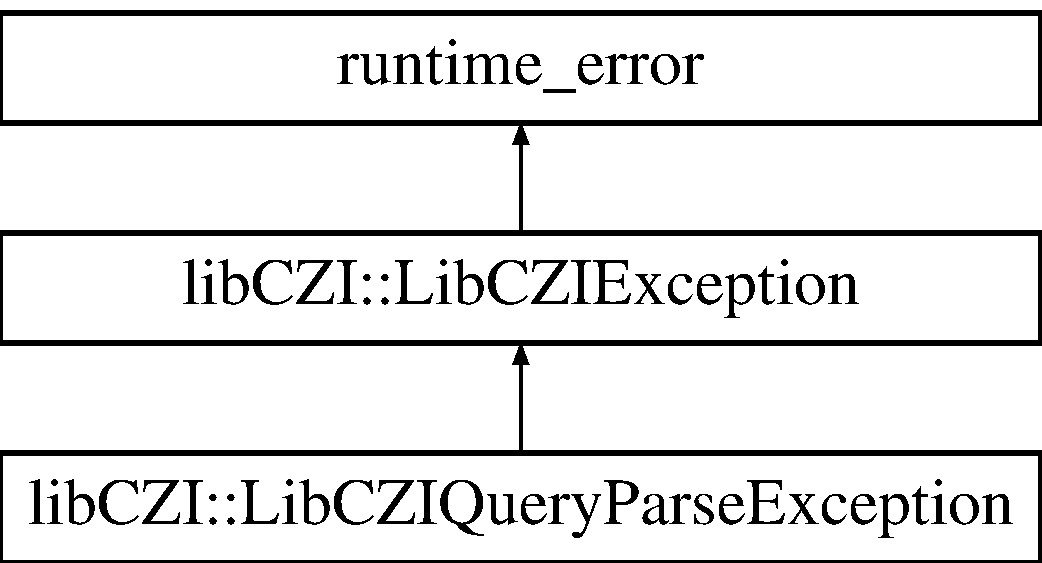
\includegraphics[height=3.000000cm]{classlib_c_z_i_1_1_lib_c_z_i_query_parse_exception}
\end{center}
\end{figure}
\subsection*{Public Types}
\begin{DoxyCompactItemize}
\item 
\mbox{\Hypertarget{classlib_c_z_i_1_1_lib_c_z_i_query_parse_exception_adf5a11c2415ec7c92d95365fa5af2fde}\label{classlib_c_z_i_1_1_lib_c_z_i_query_parse_exception_adf5a11c2415ec7c92d95365fa5af2fde}} 
enum \hyperlink{classlib_c_z_i_1_1_lib_c_z_i_query_parse_exception_adf5a11c2415ec7c92d95365fa5af2fde}{Error\+Type} \{ {\bfseries Syntax\+Error}, 
{\bfseries Unbalanced\+Parenthesis}, 
{\bfseries Illformed\+Expression}, 
{\bfseries Invalid\+Number\+Format}
 \}\begin{DoxyCompactList}\small\item\em Values that represent different error conditions. \end{DoxyCompactList}
\end{DoxyCompactItemize}
\subsection*{Public Member Functions}
\begin{DoxyCompactItemize}
\item 
\hyperlink{classlib_c_z_i_1_1_lib_c_z_i_query_parse_exception_a9c01ed75a7d690006bae37444a08a2a7}{Lib\+C\+Z\+I\+Query\+Parse\+Exception} (const char $\ast$sz\+Err\+Msg, \hyperlink{classlib_c_z_i_1_1_lib_c_z_i_query_parse_exception_adf5a11c2415ec7c92d95365fa5af2fde}{Error\+Type} error\+Type)
\item 
\hyperlink{classlib_c_z_i_1_1_lib_c_z_i_query_parse_exception_a93adeb0fad20a3c8c4ea7ba68e49d127}{Lib\+C\+Z\+I\+Query\+Parse\+Exception} (const char $\ast$sz\+Err\+Msg, \hyperlink{classlib_c_z_i_1_1_lib_c_z_i_query_parse_exception_adf5a11c2415ec7c92d95365fa5af2fde}{Error\+Type} error\+Type, int index\+Of\+Parse\+Error)
\item 
\hyperlink{classlib_c_z_i_1_1_lib_c_z_i_query_parse_exception_adf5a11c2415ec7c92d95365fa5af2fde}{Error\+Type} \hyperlink{classlib_c_z_i_1_1_lib_c_z_i_query_parse_exception_a22088facd6fc204fcaf44867bfaeb8bc}{Get\+Error\+Type} () const
\item 
int \hyperlink{classlib_c_z_i_1_1_lib_c_z_i_query_parse_exception_ae880a97ae7923437190a968d5865b86e}{Get\+Position\+After\+Which\+Parser\+Error\+Occurred} () const
\end{DoxyCompactItemize}


\subsection{Detailed Description}
Exception for signaling errors when parsing a query-\/string. 

\subsection{Constructor \& Destructor Documentation}
\mbox{\Hypertarget{classlib_c_z_i_1_1_lib_c_z_i_query_parse_exception_a9c01ed75a7d690006bae37444a08a2a7}\label{classlib_c_z_i_1_1_lib_c_z_i_query_parse_exception_a9c01ed75a7d690006bae37444a08a2a7}} 
\index{lib\+C\+Z\+I\+::\+Lib\+C\+Z\+I\+Query\+Parse\+Exception@{lib\+C\+Z\+I\+::\+Lib\+C\+Z\+I\+Query\+Parse\+Exception}!Lib\+C\+Z\+I\+Query\+Parse\+Exception@{Lib\+C\+Z\+I\+Query\+Parse\+Exception}}
\index{Lib\+C\+Z\+I\+Query\+Parse\+Exception@{Lib\+C\+Z\+I\+Query\+Parse\+Exception}!lib\+C\+Z\+I\+::\+Lib\+C\+Z\+I\+Query\+Parse\+Exception@{lib\+C\+Z\+I\+::\+Lib\+C\+Z\+I\+Query\+Parse\+Exception}}
\subsubsection{\texorpdfstring{Lib\+C\+Z\+I\+Query\+Parse\+Exception()}{LibCZIQueryParseException()}\hspace{0.1cm}{\footnotesize\ttfamily [1/2]}}
{\footnotesize\ttfamily lib\+C\+Z\+I\+::\+Lib\+C\+Z\+I\+Query\+Parse\+Exception\+::\+Lib\+C\+Z\+I\+Query\+Parse\+Exception (\begin{DoxyParamCaption}\item[{const char $\ast$}]{sz\+Err\+Msg,  }\item[{\hyperlink{classlib_c_z_i_1_1_lib_c_z_i_query_parse_exception_adf5a11c2415ec7c92d95365fa5af2fde}{Error\+Type}}]{error\+Type }\end{DoxyParamCaption})\hspace{0.3cm}{\ttfamily [inline]}}

Constructor for the Lib\+C\+Z\+I\+Query\+Parse\+Exception-\/exception. This exception is used to signal errors when parsing a query-\/string. 
\begin{DoxyParams}{Parameters}
{\em sz\+Err\+Msg} & Message describing the error. \\
\hline
{\em error\+Type} & Type of the error. \\
\hline
\end{DoxyParams}
\mbox{\Hypertarget{classlib_c_z_i_1_1_lib_c_z_i_query_parse_exception_a93adeb0fad20a3c8c4ea7ba68e49d127}\label{classlib_c_z_i_1_1_lib_c_z_i_query_parse_exception_a93adeb0fad20a3c8c4ea7ba68e49d127}} 
\index{lib\+C\+Z\+I\+::\+Lib\+C\+Z\+I\+Query\+Parse\+Exception@{lib\+C\+Z\+I\+::\+Lib\+C\+Z\+I\+Query\+Parse\+Exception}!Lib\+C\+Z\+I\+Query\+Parse\+Exception@{Lib\+C\+Z\+I\+Query\+Parse\+Exception}}
\index{Lib\+C\+Z\+I\+Query\+Parse\+Exception@{Lib\+C\+Z\+I\+Query\+Parse\+Exception}!lib\+C\+Z\+I\+::\+Lib\+C\+Z\+I\+Query\+Parse\+Exception@{lib\+C\+Z\+I\+::\+Lib\+C\+Z\+I\+Query\+Parse\+Exception}}
\subsubsection{\texorpdfstring{Lib\+C\+Z\+I\+Query\+Parse\+Exception()}{LibCZIQueryParseException()}\hspace{0.1cm}{\footnotesize\ttfamily [2/2]}}
{\footnotesize\ttfamily lib\+C\+Z\+I\+::\+Lib\+C\+Z\+I\+Query\+Parse\+Exception\+::\+Lib\+C\+Z\+I\+Query\+Parse\+Exception (\begin{DoxyParamCaption}\item[{const char $\ast$}]{sz\+Err\+Msg,  }\item[{\hyperlink{classlib_c_z_i_1_1_lib_c_z_i_query_parse_exception_adf5a11c2415ec7c92d95365fa5af2fde}{Error\+Type}}]{error\+Type,  }\item[{int}]{index\+Of\+Parse\+Error }\end{DoxyParamCaption})\hspace{0.3cm}{\ttfamily [inline]}, {\ttfamily [explicit]}}

Constructor for the Lib\+C\+Z\+I\+Query\+Parse\+Exception-\/exception. This exception is used to signal errors when parsing a query-\/string. 
\begin{DoxyParams}{Parameters}
{\em sz\+Err\+Msg} & Message describing the error. \\
\hline
{\em error\+Type} & Type of the error. \\
\hline
{\em index\+Of\+Parse\+Error} & The index to the character of the query string where the error was detected. If negative, this value is not valid. \\
\hline
\end{DoxyParams}


\subsection{Member Function Documentation}
\mbox{\Hypertarget{classlib_c_z_i_1_1_lib_c_z_i_query_parse_exception_a22088facd6fc204fcaf44867bfaeb8bc}\label{classlib_c_z_i_1_1_lib_c_z_i_query_parse_exception_a22088facd6fc204fcaf44867bfaeb8bc}} 
\index{lib\+C\+Z\+I\+::\+Lib\+C\+Z\+I\+Query\+Parse\+Exception@{lib\+C\+Z\+I\+::\+Lib\+C\+Z\+I\+Query\+Parse\+Exception}!Get\+Error\+Type@{Get\+Error\+Type}}
\index{Get\+Error\+Type@{Get\+Error\+Type}!lib\+C\+Z\+I\+::\+Lib\+C\+Z\+I\+Query\+Parse\+Exception@{lib\+C\+Z\+I\+::\+Lib\+C\+Z\+I\+Query\+Parse\+Exception}}
\subsubsection{\texorpdfstring{Get\+Error\+Type()}{GetErrorType()}}
{\footnotesize\ttfamily \hyperlink{classlib_c_z_i_1_1_lib_c_z_i_query_parse_exception_adf5a11c2415ec7c92d95365fa5af2fde}{Error\+Type} lib\+C\+Z\+I\+::\+Lib\+C\+Z\+I\+Query\+Parse\+Exception\+::\+Get\+Error\+Type (\begin{DoxyParamCaption}{ }\end{DoxyParamCaption}) const\hspace{0.3cm}{\ttfamily [inline]}}

Gets error type \begin{DoxyReturn}{Returns}
The error type. 
\end{DoxyReturn}
\mbox{\Hypertarget{classlib_c_z_i_1_1_lib_c_z_i_query_parse_exception_ae880a97ae7923437190a968d5865b86e}\label{classlib_c_z_i_1_1_lib_c_z_i_query_parse_exception_ae880a97ae7923437190a968d5865b86e}} 
\index{lib\+C\+Z\+I\+::\+Lib\+C\+Z\+I\+Query\+Parse\+Exception@{lib\+C\+Z\+I\+::\+Lib\+C\+Z\+I\+Query\+Parse\+Exception}!Get\+Position\+After\+Which\+Parser\+Error\+Occurred@{Get\+Position\+After\+Which\+Parser\+Error\+Occurred}}
\index{Get\+Position\+After\+Which\+Parser\+Error\+Occurred@{Get\+Position\+After\+Which\+Parser\+Error\+Occurred}!lib\+C\+Z\+I\+::\+Lib\+C\+Z\+I\+Query\+Parse\+Exception@{lib\+C\+Z\+I\+::\+Lib\+C\+Z\+I\+Query\+Parse\+Exception}}
\subsubsection{\texorpdfstring{Get\+Position\+After\+Which\+Parser\+Error\+Occurred()}{GetPositionAfterWhichParserErrorOccurred()}}
{\footnotesize\ttfamily int lib\+C\+Z\+I\+::\+Lib\+C\+Z\+I\+Query\+Parse\+Exception\+::\+Get\+Position\+After\+Which\+Parser\+Error\+Occurred (\begin{DoxyParamCaption}{ }\end{DoxyParamCaption}) const\hspace{0.3cm}{\ttfamily [inline]}}

Gets position of the character in the query-\/string after which the parser error occurred. If negative, this value is not valid. \begin{DoxyReturn}{Returns}
The position after which parser error occurred. 
\end{DoxyReturn}


The documentation for this class was generated from the following file\+:\begin{DoxyCompactItemize}
\item 
lib\+C\+Z\+I/lib\+C\+Z\+I\+\_\+exceptions.\+h\end{DoxyCompactItemize}

\hypertarget{classlib_c_z_i_1_1_lib_c_z_i_string_parse_exception}{}\section{lib\+C\+ZI\+:\+:Lib\+C\+Z\+I\+String\+Parse\+Exception Class Reference}
\label{classlib_c_z_i_1_1_lib_c_z_i_string_parse_exception}\index{lib\+C\+Z\+I\+::\+Lib\+C\+Z\+I\+String\+Parse\+Exception@{lib\+C\+Z\+I\+::\+Lib\+C\+Z\+I\+String\+Parse\+Exception}}


Exception for signaling that a string did not parse correctly.  




{\ttfamily \#include $<$lib\+C\+Z\+I\+\_\+exceptions.\+h$>$}

Inheritance diagram for lib\+C\+ZI\+:\+:Lib\+C\+Z\+I\+String\+Parse\+Exception\+:\begin{figure}[H]
\begin{center}
\leavevmode
\includegraphics[height=3.000000cm]{classlib_c_z_i_1_1_lib_c_z_i_string_parse_exception}
\end{center}
\end{figure}
\subsection*{Public Types}
\begin{DoxyCompactItemize}
\item 
enum \hyperlink{classlib_c_z_i_1_1_lib_c_z_i_string_parse_exception_a42ecdd87f0e6f47ca0accda1b90497d2}{Error\+Type} \{ \hyperlink{classlib_c_z_i_1_1_lib_c_z_i_string_parse_exception_a42ecdd87f0e6f47ca0accda1b90497d2afc52000b95d50ca5da692212b69e61c2}{Error\+Type\+::\+Invalid\+Syntax}, 
\hyperlink{classlib_c_z_i_1_1_lib_c_z_i_string_parse_exception_a42ecdd87f0e6f47ca0accda1b90497d2a6a381f451ea053e25a0e87136e35dd19}{Error\+Type\+::\+Duplicate\+Dimension}, 
\hyperlink{classlib_c_z_i_1_1_lib_c_z_i_string_parse_exception_a42ecdd87f0e6f47ca0accda1b90497d2aff73eb7f68565f16f023d1c074816ea5}{Error\+Type\+::\+From\+Greater\+Than\+To}, 
\hyperlink{classlib_c_z_i_1_1_lib_c_z_i_string_parse_exception_a42ecdd87f0e6f47ca0accda1b90497d2a6fcdc090caeade09d0efd6253932b6f5}{Error\+Type\+::\+Unspecified}
 \}\begin{DoxyCompactList}\small\item\em Values that represent error types. \end{DoxyCompactList}
\end{DoxyCompactItemize}
\subsection*{Public Member Functions}
\begin{DoxyCompactItemize}
\item 
\hyperlink{classlib_c_z_i_1_1_lib_c_z_i_string_parse_exception_a6bcf9792770dc4cbe17f8a8a0d665b7d}{Lib\+C\+Z\+I\+String\+Parse\+Exception} (const char $\ast$sz\+Err\+Msg, int number\+Of\+Chars\+Parsed\+Ok, \hyperlink{classlib_c_z_i_1_1_lib_c_z_i_string_parse_exception_a42ecdd87f0e6f47ca0accda1b90497d2}{Error\+Type} error\+Type)
\item 
\hyperlink{classlib_c_z_i_1_1_lib_c_z_i_string_parse_exception_a42ecdd87f0e6f47ca0accda1b90497d2}{Error\+Type} \hyperlink{classlib_c_z_i_1_1_lib_c_z_i_string_parse_exception_abf18d7eb523f8aa3ed8b110e2cc170a2}{Get\+Error\+Type} () const
\item 
int \hyperlink{classlib_c_z_i_1_1_lib_c_z_i_string_parse_exception_ab9f93bffdad9f93cec7d69f66ce57dfc}{Get\+Number\+Of\+Chars\+Parsed\+Ok} () const
\end{DoxyCompactItemize}


\subsection{Detailed Description}
Exception for signaling that a string did not parse correctly. 

\subsection{Member Enumeration Documentation}
\mbox{\Hypertarget{classlib_c_z_i_1_1_lib_c_z_i_string_parse_exception_a42ecdd87f0e6f47ca0accda1b90497d2}\label{classlib_c_z_i_1_1_lib_c_z_i_string_parse_exception_a42ecdd87f0e6f47ca0accda1b90497d2}} 
\index{lib\+C\+Z\+I\+::\+Lib\+C\+Z\+I\+String\+Parse\+Exception@{lib\+C\+Z\+I\+::\+Lib\+C\+Z\+I\+String\+Parse\+Exception}!Error\+Type@{Error\+Type}}
\index{Error\+Type@{Error\+Type}!lib\+C\+Z\+I\+::\+Lib\+C\+Z\+I\+String\+Parse\+Exception@{lib\+C\+Z\+I\+::\+Lib\+C\+Z\+I\+String\+Parse\+Exception}}
\subsubsection{\texorpdfstring{Error\+Type}{ErrorType}}
{\footnotesize\ttfamily enum \hyperlink{classlib_c_z_i_1_1_lib_c_z_i_string_parse_exception_a42ecdd87f0e6f47ca0accda1b90497d2}{lib\+C\+Z\+I\+::\+Lib\+C\+Z\+I\+String\+Parse\+Exception\+::\+Error\+Type}\hspace{0.3cm}{\ttfamily [strong]}}



Values that represent error types. 

\begin{DoxyEnumFields}{Enumerator}
\raisebox{\heightof{T}}[0pt][0pt]{\index{Invalid\+Syntax@{Invalid\+Syntax}!lib\+C\+Z\+I\+::\+Lib\+C\+Z\+I\+String\+Parse\+Exception@{lib\+C\+Z\+I\+::\+Lib\+C\+Z\+I\+String\+Parse\+Exception}}\index{lib\+C\+Z\+I\+::\+Lib\+C\+Z\+I\+String\+Parse\+Exception@{lib\+C\+Z\+I\+::\+Lib\+C\+Z\+I\+String\+Parse\+Exception}!Invalid\+Syntax@{Invalid\+Syntax}}}\mbox{\Hypertarget{classlib_c_z_i_1_1_lib_c_z_i_string_parse_exception_a42ecdd87f0e6f47ca0accda1b90497d2afc52000b95d50ca5da692212b69e61c2}\label{classlib_c_z_i_1_1_lib_c_z_i_string_parse_exception_a42ecdd87f0e6f47ca0accda1b90497d2afc52000b95d50ca5da692212b69e61c2}} 
Invalid\+Syntax&The string parsed has an invalid syntax. \\
\hline

\raisebox{\heightof{T}}[0pt][0pt]{\index{Duplicate\+Dimension@{Duplicate\+Dimension}!lib\+C\+Z\+I\+::\+Lib\+C\+Z\+I\+String\+Parse\+Exception@{lib\+C\+Z\+I\+::\+Lib\+C\+Z\+I\+String\+Parse\+Exception}}\index{lib\+C\+Z\+I\+::\+Lib\+C\+Z\+I\+String\+Parse\+Exception@{lib\+C\+Z\+I\+::\+Lib\+C\+Z\+I\+String\+Parse\+Exception}!Duplicate\+Dimension@{Duplicate\+Dimension}}}\mbox{\Hypertarget{classlib_c_z_i_1_1_lib_c_z_i_string_parse_exception_a42ecdd87f0e6f47ca0accda1b90497d2a6a381f451ea053e25a0e87136e35dd19}\label{classlib_c_z_i_1_1_lib_c_z_i_string_parse_exception_a42ecdd87f0e6f47ca0accda1b90497d2a6a381f451ea053e25a0e87136e35dd19}} 
Duplicate\+Dimension&When parsing a string representation of a coordinate, it was detected, that a dimension occured more than once. \\
\hline

\raisebox{\heightof{T}}[0pt][0pt]{\index{From\+Greater\+Than\+To@{From\+Greater\+Than\+To}!lib\+C\+Z\+I\+::\+Lib\+C\+Z\+I\+String\+Parse\+Exception@{lib\+C\+Z\+I\+::\+Lib\+C\+Z\+I\+String\+Parse\+Exception}}\index{lib\+C\+Z\+I\+::\+Lib\+C\+Z\+I\+String\+Parse\+Exception@{lib\+C\+Z\+I\+::\+Lib\+C\+Z\+I\+String\+Parse\+Exception}!From\+Greater\+Than\+To@{From\+Greater\+Than\+To}}}\mbox{\Hypertarget{classlib_c_z_i_1_1_lib_c_z_i_string_parse_exception_a42ecdd87f0e6f47ca0accda1b90497d2aff73eb7f68565f16f023d1c074816ea5}\label{classlib_c_z_i_1_1_lib_c_z_i_string_parse_exception_a42ecdd87f0e6f47ca0accda1b90497d2aff73eb7f68565f16f023d1c074816ea5}} 
From\+Greater\+Than\+To&A range was parsed, and the start value is bigger than the end value. \\
\hline

\raisebox{\heightof{T}}[0pt][0pt]{\index{Unspecified@{Unspecified}!lib\+C\+Z\+I\+::\+Lib\+C\+Z\+I\+String\+Parse\+Exception@{lib\+C\+Z\+I\+::\+Lib\+C\+Z\+I\+String\+Parse\+Exception}}\index{lib\+C\+Z\+I\+::\+Lib\+C\+Z\+I\+String\+Parse\+Exception@{lib\+C\+Z\+I\+::\+Lib\+C\+Z\+I\+String\+Parse\+Exception}!Unspecified@{Unspecified}}}\mbox{\Hypertarget{classlib_c_z_i_1_1_lib_c_z_i_string_parse_exception_a42ecdd87f0e6f47ca0accda1b90497d2a6fcdc090caeade09d0efd6253932b6f5}\label{classlib_c_z_i_1_1_lib_c_z_i_string_parse_exception_a42ecdd87f0e6f47ca0accda1b90497d2a6fcdc090caeade09d0efd6253932b6f5}} 
Unspecified&General error. \\
\hline

\end{DoxyEnumFields}


\subsection{Constructor \& Destructor Documentation}
\mbox{\Hypertarget{classlib_c_z_i_1_1_lib_c_z_i_string_parse_exception_a6bcf9792770dc4cbe17f8a8a0d665b7d}\label{classlib_c_z_i_1_1_lib_c_z_i_string_parse_exception_a6bcf9792770dc4cbe17f8a8a0d665b7d}} 
\index{lib\+C\+Z\+I\+::\+Lib\+C\+Z\+I\+String\+Parse\+Exception@{lib\+C\+Z\+I\+::\+Lib\+C\+Z\+I\+String\+Parse\+Exception}!Lib\+C\+Z\+I\+String\+Parse\+Exception@{Lib\+C\+Z\+I\+String\+Parse\+Exception}}
\index{Lib\+C\+Z\+I\+String\+Parse\+Exception@{Lib\+C\+Z\+I\+String\+Parse\+Exception}!lib\+C\+Z\+I\+::\+Lib\+C\+Z\+I\+String\+Parse\+Exception@{lib\+C\+Z\+I\+::\+Lib\+C\+Z\+I\+String\+Parse\+Exception}}
\subsubsection{\texorpdfstring{Lib\+C\+Z\+I\+String\+Parse\+Exception()}{LibCZIStringParseException()}}
{\footnotesize\ttfamily lib\+C\+Z\+I\+::\+Lib\+C\+Z\+I\+String\+Parse\+Exception\+::\+Lib\+C\+Z\+I\+String\+Parse\+Exception (\begin{DoxyParamCaption}\item[{const char $\ast$}]{sz\+Err\+Msg,  }\item[{int}]{number\+Of\+Chars\+Parsed\+Ok,  }\item[{\hyperlink{classlib_c_z_i_1_1_lib_c_z_i_string_parse_exception_a42ecdd87f0e6f47ca0accda1b90497d2}{Error\+Type}}]{error\+Type }\end{DoxyParamCaption})\hspace{0.3cm}{\ttfamily [inline]}}

Constructor for the \hyperlink{classlib_c_z_i_1_1_lib_c_z_i_string_parse_exception}{Lib\+C\+Z\+I\+String\+Parse\+Exception}. This type is used to signal that a string did not parse correctly. 
\begin{DoxyParams}{Parameters}
{\em sz\+Err\+Msg} & Message describing the error. \\
\hline
{\em number\+Of\+Chars\+Parsed\+Ok} & Number of characters parsed ok. The parse error occured after this position. If negative, then this information is not available. \\
\hline
{\em error\+Type} & Type of the error. \\
\hline
\end{DoxyParams}


\subsection{Member Function Documentation}
\mbox{\Hypertarget{classlib_c_z_i_1_1_lib_c_z_i_string_parse_exception_abf18d7eb523f8aa3ed8b110e2cc170a2}\label{classlib_c_z_i_1_1_lib_c_z_i_string_parse_exception_abf18d7eb523f8aa3ed8b110e2cc170a2}} 
\index{lib\+C\+Z\+I\+::\+Lib\+C\+Z\+I\+String\+Parse\+Exception@{lib\+C\+Z\+I\+::\+Lib\+C\+Z\+I\+String\+Parse\+Exception}!Get\+Error\+Type@{Get\+Error\+Type}}
\index{Get\+Error\+Type@{Get\+Error\+Type}!lib\+C\+Z\+I\+::\+Lib\+C\+Z\+I\+String\+Parse\+Exception@{lib\+C\+Z\+I\+::\+Lib\+C\+Z\+I\+String\+Parse\+Exception}}
\subsubsection{\texorpdfstring{Get\+Error\+Type()}{GetErrorType()}}
{\footnotesize\ttfamily \hyperlink{classlib_c_z_i_1_1_lib_c_z_i_string_parse_exception_a42ecdd87f0e6f47ca0accda1b90497d2}{Error\+Type} lib\+C\+Z\+I\+::\+Lib\+C\+Z\+I\+String\+Parse\+Exception\+::\+Get\+Error\+Type (\begin{DoxyParamCaption}{ }\end{DoxyParamCaption}) const\hspace{0.3cm}{\ttfamily [inline]}}

Gets error type. \begin{DoxyReturn}{Returns}
The error type. 
\end{DoxyReturn}
\mbox{\Hypertarget{classlib_c_z_i_1_1_lib_c_z_i_string_parse_exception_ab9f93bffdad9f93cec7d69f66ce57dfc}\label{classlib_c_z_i_1_1_lib_c_z_i_string_parse_exception_ab9f93bffdad9f93cec7d69f66ce57dfc}} 
\index{lib\+C\+Z\+I\+::\+Lib\+C\+Z\+I\+String\+Parse\+Exception@{lib\+C\+Z\+I\+::\+Lib\+C\+Z\+I\+String\+Parse\+Exception}!Get\+Number\+Of\+Chars\+Parsed\+Ok@{Get\+Number\+Of\+Chars\+Parsed\+Ok}}
\index{Get\+Number\+Of\+Chars\+Parsed\+Ok@{Get\+Number\+Of\+Chars\+Parsed\+Ok}!lib\+C\+Z\+I\+::\+Lib\+C\+Z\+I\+String\+Parse\+Exception@{lib\+C\+Z\+I\+::\+Lib\+C\+Z\+I\+String\+Parse\+Exception}}
\subsubsection{\texorpdfstring{Get\+Number\+Of\+Chars\+Parsed\+Ok()}{GetNumberOfCharsParsedOk()}}
{\footnotesize\ttfamily int lib\+C\+Z\+I\+::\+Lib\+C\+Z\+I\+String\+Parse\+Exception\+::\+Get\+Number\+Of\+Chars\+Parsed\+Ok (\begin{DoxyParamCaption}{ }\end{DoxyParamCaption}) const\hspace{0.3cm}{\ttfamily [inline]}}

Gets number of characters that parsed correctly. The parse error occured after this position. If this number is negative, then this information is not available and valid. \begin{DoxyReturn}{Returns}
The number of characters parsed that parsed correctly. If the number is negative, this information is not available. 
\end{DoxyReturn}


The documentation for this class was generated from the following file\+:\begin{DoxyCompactItemize}
\item 
lib\+C\+Z\+I/lib\+C\+Z\+I\+\_\+exceptions.\+h\end{DoxyCompactItemize}

\hypertarget{classlib_c_z_i_1_1_lib_c_z_i_xml_parse_exception}{}\section{lib\+C\+ZI\+:\+:Lib\+C\+Z\+I\+Xml\+Parse\+Exception Class Reference}
\label{classlib_c_z_i_1_1_lib_c_z_i_xml_parse_exception}\index{lib\+C\+Z\+I\+::\+Lib\+C\+Z\+I\+Xml\+Parse\+Exception@{lib\+C\+Z\+I\+::\+Lib\+C\+Z\+I\+Xml\+Parse\+Exception}}


Exception for signaling errors when parsing the X\+M\+L-\/metadata.  




{\ttfamily \#include $<$lib\+C\+Z\+I\+\_\+exceptions.\+h$>$}

Inheritance diagram for lib\+C\+ZI\+:\+:Lib\+C\+Z\+I\+Xml\+Parse\+Exception\+:\begin{figure}[H]
\begin{center}
\leavevmode
\includegraphics[height=3.000000cm]{classlib_c_z_i_1_1_lib_c_z_i_xml_parse_exception}
\end{center}
\end{figure}
\subsection*{Public Member Functions}
\begin{DoxyCompactItemize}
\item 
\hyperlink{classlib_c_z_i_1_1_lib_c_z_i_xml_parse_exception_adfe0a6c32d816bd079e668534c619648}{Lib\+C\+Z\+I\+Xml\+Parse\+Exception} (const char $\ast$sz\+Err\+Msg)
\end{DoxyCompactItemize}


\subsection{Detailed Description}
Exception for signaling errors when parsing the X\+M\+L-\/metadata. 

\subsection{Constructor \& Destructor Documentation}
\mbox{\Hypertarget{classlib_c_z_i_1_1_lib_c_z_i_xml_parse_exception_adfe0a6c32d816bd079e668534c619648}\label{classlib_c_z_i_1_1_lib_c_z_i_xml_parse_exception_adfe0a6c32d816bd079e668534c619648}} 
\index{lib\+C\+Z\+I\+::\+Lib\+C\+Z\+I\+Xml\+Parse\+Exception@{lib\+C\+Z\+I\+::\+Lib\+C\+Z\+I\+Xml\+Parse\+Exception}!Lib\+C\+Z\+I\+Xml\+Parse\+Exception@{Lib\+C\+Z\+I\+Xml\+Parse\+Exception}}
\index{Lib\+C\+Z\+I\+Xml\+Parse\+Exception@{Lib\+C\+Z\+I\+Xml\+Parse\+Exception}!lib\+C\+Z\+I\+::\+Lib\+C\+Z\+I\+Xml\+Parse\+Exception@{lib\+C\+Z\+I\+::\+Lib\+C\+Z\+I\+Xml\+Parse\+Exception}}
\subsubsection{\texorpdfstring{Lib\+C\+Z\+I\+Xml\+Parse\+Exception()}{LibCZIXmlParseException()}}
{\footnotesize\ttfamily lib\+C\+Z\+I\+::\+Lib\+C\+Z\+I\+Xml\+Parse\+Exception\+::\+Lib\+C\+Z\+I\+Xml\+Parse\+Exception (\begin{DoxyParamCaption}\item[{const char $\ast$}]{sz\+Err\+Msg }\end{DoxyParamCaption})\hspace{0.3cm}{\ttfamily [inline]}}

Constructor for the \hyperlink{classlib_c_z_i_1_1_lib_c_z_i_xml_parse_exception}{Lib\+C\+Z\+I\+Xml\+Parse\+Exception}. This type is used signaling errors when parsing the X\+M\+L-\/metadata. 
\begin{DoxyParams}{Parameters}
{\em sz\+Err\+Msg} & Message describing the error. \\
\hline
\end{DoxyParams}


The documentation for this class was generated from the following file\+:\begin{DoxyCompactItemize}
\item 
lib\+C\+Z\+I/lib\+C\+Z\+I\+\_\+exceptions.\+h\end{DoxyCompactItemize}

\hypertarget{structlib_c_z_i_1_1_i_single_channel_scaling_tile_accessor_1_1_options}{}\section{lib\+C\+ZI\+:\+:I\+Single\+Channel\+Scaling\+Tile\+Accessor\+:\+:Options Struct Reference}
\label{structlib_c_z_i_1_1_i_single_channel_scaling_tile_accessor_1_1_options}\index{lib\+C\+Z\+I\+::\+I\+Single\+Channel\+Scaling\+Tile\+Accessor\+::\+Options@{lib\+C\+Z\+I\+::\+I\+Single\+Channel\+Scaling\+Tile\+Accessor\+::\+Options}}


\hyperlink{structlib_c_z_i_1_1_i_single_channel_scaling_tile_accessor_1_1_options}{Options} used for this accessor.  




{\ttfamily \#include $<$lib\+C\+Z\+I\+\_\+\+Compositor.\+h$>$}

\subsection*{Public Member Functions}
\begin{DoxyCompactItemize}
\item 
\mbox{\Hypertarget{structlib_c_z_i_1_1_i_single_channel_scaling_tile_accessor_1_1_options_a62bce09e0eb8da84c26106b183c6d338}\label{structlib_c_z_i_1_1_i_single_channel_scaling_tile_accessor_1_1_options_a62bce09e0eb8da84c26106b183c6d338}} 
void \hyperlink{structlib_c_z_i_1_1_i_single_channel_scaling_tile_accessor_1_1_options_a62bce09e0eb8da84c26106b183c6d338}{Clear} ()
\begin{DoxyCompactList}\small\item\em Clears this object to its blank state. \end{DoxyCompactList}\end{DoxyCompactItemize}
\subsection*{Public Attributes}
\begin{DoxyCompactItemize}
\item 
\hyperlink{structlib_c_z_i_1_1_rgb_float_color}{Rgb\+Float\+Color} \hyperlink{structlib_c_z_i_1_1_i_single_channel_scaling_tile_accessor_1_1_options_a2d62a4b7e8dd4edc3d4419c2dc3e4901}{back\+Ground\+Color}
\item 
bool \hyperlink{structlib_c_z_i_1_1_i_single_channel_scaling_tile_accessor_1_1_options_ad0ff6bfe4369dd315edc4cfca9747596}{draw\+Tile\+Border}
\item 
\mbox{\Hypertarget{structlib_c_z_i_1_1_i_single_channel_scaling_tile_accessor_1_1_options_a8cede93cd20a293ccf34354813779d41}\label{structlib_c_z_i_1_1_i_single_channel_scaling_tile_accessor_1_1_options_a8cede93cd20a293ccf34354813779d41}} 
std\+::shared\+\_\+ptr$<$ \hyperlink{classlib_c_z_i_1_1_i_index_set}{lib\+C\+Z\+I\+::\+I\+Index\+Set} $>$ \hyperlink{structlib_c_z_i_1_1_i_single_channel_scaling_tile_accessor_1_1_options_a8cede93cd20a293ccf34354813779d41}{scene\+Filter}
\begin{DoxyCompactList}\small\item\em If specified, only subblocks with a scene-\/index contained in the set will be considered. \end{DoxyCompactList}\end{DoxyCompactItemize}


\subsection{Detailed Description}
\hyperlink{structlib_c_z_i_1_1_i_single_channel_scaling_tile_accessor_1_1_options}{Options} used for this accessor. 

\subsection{Member Data Documentation}
\mbox{\Hypertarget{structlib_c_z_i_1_1_i_single_channel_scaling_tile_accessor_1_1_options_a2d62a4b7e8dd4edc3d4419c2dc3e4901}\label{structlib_c_z_i_1_1_i_single_channel_scaling_tile_accessor_1_1_options_a2d62a4b7e8dd4edc3d4419c2dc3e4901}} 
\index{lib\+C\+Z\+I\+::\+I\+Single\+Channel\+Scaling\+Tile\+Accessor\+::\+Options@{lib\+C\+Z\+I\+::\+I\+Single\+Channel\+Scaling\+Tile\+Accessor\+::\+Options}!back\+Ground\+Color@{back\+Ground\+Color}}
\index{back\+Ground\+Color@{back\+Ground\+Color}!lib\+C\+Z\+I\+::\+I\+Single\+Channel\+Scaling\+Tile\+Accessor\+::\+Options@{lib\+C\+Z\+I\+::\+I\+Single\+Channel\+Scaling\+Tile\+Accessor\+::\+Options}}
\subsubsection{\texorpdfstring{back\+Ground\+Color}{backGroundColor}}
{\footnotesize\ttfamily \hyperlink{structlib_c_z_i_1_1_rgb_float_color}{Rgb\+Float\+Color} lib\+C\+Z\+I\+::\+I\+Single\+Channel\+Scaling\+Tile\+Accessor\+::\+Options\+::back\+Ground\+Color}

The back ground color. If the destination bitmap is a grayscale-\/type, then the mean from R, G and B is calculated and multiplied with the maximum pixel value (of the specific pixeltype). If it is a R\+G\+B-\/color type, then R, G and B are separately multiplied with the maximum pixel value. If any of R, G or B is NaN, then the background is not cleared. \mbox{\Hypertarget{structlib_c_z_i_1_1_i_single_channel_scaling_tile_accessor_1_1_options_ad0ff6bfe4369dd315edc4cfca9747596}\label{structlib_c_z_i_1_1_i_single_channel_scaling_tile_accessor_1_1_options_ad0ff6bfe4369dd315edc4cfca9747596}} 
\index{lib\+C\+Z\+I\+::\+I\+Single\+Channel\+Scaling\+Tile\+Accessor\+::\+Options@{lib\+C\+Z\+I\+::\+I\+Single\+Channel\+Scaling\+Tile\+Accessor\+::\+Options}!draw\+Tile\+Border@{draw\+Tile\+Border}}
\index{draw\+Tile\+Border@{draw\+Tile\+Border}!lib\+C\+Z\+I\+::\+I\+Single\+Channel\+Scaling\+Tile\+Accessor\+::\+Options@{lib\+C\+Z\+I\+::\+I\+Single\+Channel\+Scaling\+Tile\+Accessor\+::\+Options}}
\subsubsection{\texorpdfstring{draw\+Tile\+Border}{drawTileBorder}}
{\footnotesize\ttfamily bool lib\+C\+Z\+I\+::\+I\+Single\+Channel\+Scaling\+Tile\+Accessor\+::\+Options\+::draw\+Tile\+Border}

If true, then a one-\/pixel wide boundary will be drawn around each tile (in black color). 

The documentation for this struct was generated from the following file\+:\begin{DoxyCompactItemize}
\item 
lib\+C\+Z\+I/lib\+C\+Z\+I\+\_\+\+Compositor.\+h\end{DoxyCompactItemize}

\hypertarget{structlib_c_z_i_1_1_i_single_channel_tile_accessor_1_1_options}{}\section{lib\+C\+ZI\+:\+:I\+Single\+Channel\+Tile\+Accessor\+:\+:Options Struct Reference}
\label{structlib_c_z_i_1_1_i_single_channel_tile_accessor_1_1_options}\index{lib\+C\+Z\+I\+::\+I\+Single\+Channel\+Tile\+Accessor\+::\+Options@{lib\+C\+Z\+I\+::\+I\+Single\+Channel\+Tile\+Accessor\+::\+Options}}


\hyperlink{structlib_c_z_i_1_1_i_single_channel_tile_accessor_1_1_options}{Options} for controlling the composition operation.  




{\ttfamily \#include $<$lib\+C\+Z\+I\+\_\+\+Compositor.\+h$>$}

\subsection*{Public Member Functions}
\begin{DoxyCompactItemize}
\item 
\mbox{\Hypertarget{structlib_c_z_i_1_1_i_single_channel_tile_accessor_1_1_options_a8a71ed70115175973da1251e01ddf838}\label{structlib_c_z_i_1_1_i_single_channel_tile_accessor_1_1_options_a8a71ed70115175973da1251e01ddf838}} 
void \hyperlink{structlib_c_z_i_1_1_i_single_channel_tile_accessor_1_1_options_a8a71ed70115175973da1251e01ddf838}{Clear} ()
\begin{DoxyCompactList}\small\item\em Clears this object to its blank state. \end{DoxyCompactList}\end{DoxyCompactItemize}
\subsection*{Public Attributes}
\begin{DoxyCompactItemize}
\item 
\hyperlink{structlib_c_z_i_1_1_rgb_float_color}{Rgb\+Float\+Color} \hyperlink{structlib_c_z_i_1_1_i_single_channel_tile_accessor_1_1_options_a55c96574134736e35182931d4bee4636}{back\+Ground\+Color}
\item 
bool \hyperlink{structlib_c_z_i_1_1_i_single_channel_tile_accessor_1_1_options_a6825901b1c28cff524d5eec48a2ceea3}{sort\+ByM}
\item 
bool \hyperlink{structlib_c_z_i_1_1_i_single_channel_tile_accessor_1_1_options_aa1d7947be1a24339a446efbeb371d34d}{draw\+Tile\+Border}
\item 
\mbox{\Hypertarget{structlib_c_z_i_1_1_i_single_channel_tile_accessor_1_1_options_a7f07fd78043d3ab587e86a510a088e84}\label{structlib_c_z_i_1_1_i_single_channel_tile_accessor_1_1_options_a7f07fd78043d3ab587e86a510a088e84}} 
std\+::shared\+\_\+ptr$<$ \hyperlink{classlib_c_z_i_1_1_i_index_set}{lib\+C\+Z\+I\+::\+I\+Index\+Set} $>$ \hyperlink{structlib_c_z_i_1_1_i_single_channel_tile_accessor_1_1_options_a7f07fd78043d3ab587e86a510a088e84}{scene\+Filter}
\begin{DoxyCompactList}\small\item\em If specified, only subblocks with a scene-\/index contained in the set will be considered. \end{DoxyCompactList}\end{DoxyCompactItemize}


\subsection{Detailed Description}
\hyperlink{structlib_c_z_i_1_1_i_single_channel_tile_accessor_1_1_options}{Options} for controlling the composition operation. 

\subsection{Member Data Documentation}
\mbox{\Hypertarget{structlib_c_z_i_1_1_i_single_channel_tile_accessor_1_1_options_a55c96574134736e35182931d4bee4636}\label{structlib_c_z_i_1_1_i_single_channel_tile_accessor_1_1_options_a55c96574134736e35182931d4bee4636}} 
\index{lib\+C\+Z\+I\+::\+I\+Single\+Channel\+Tile\+Accessor\+::\+Options@{lib\+C\+Z\+I\+::\+I\+Single\+Channel\+Tile\+Accessor\+::\+Options}!back\+Ground\+Color@{back\+Ground\+Color}}
\index{back\+Ground\+Color@{back\+Ground\+Color}!lib\+C\+Z\+I\+::\+I\+Single\+Channel\+Tile\+Accessor\+::\+Options@{lib\+C\+Z\+I\+::\+I\+Single\+Channel\+Tile\+Accessor\+::\+Options}}
\subsubsection{\texorpdfstring{back\+Ground\+Color}{backGroundColor}}
{\footnotesize\ttfamily \hyperlink{structlib_c_z_i_1_1_rgb_float_color}{Rgb\+Float\+Color} lib\+C\+Z\+I\+::\+I\+Single\+Channel\+Tile\+Accessor\+::\+Options\+::back\+Ground\+Color}

The back ground color. If the destination bitmap is a grayscale-\/type, then the mean from R, G and B is calculated and multiplied with the maximum pixel value (of the specific pixeltype). If it is a R\+G\+B-\/color type, then R, G and B are separately multiplied with the maximum pixel value. If any of R, G or B is NaN, then the background is not cleared. \mbox{\Hypertarget{structlib_c_z_i_1_1_i_single_channel_tile_accessor_1_1_options_aa1d7947be1a24339a446efbeb371d34d}\label{structlib_c_z_i_1_1_i_single_channel_tile_accessor_1_1_options_aa1d7947be1a24339a446efbeb371d34d}} 
\index{lib\+C\+Z\+I\+::\+I\+Single\+Channel\+Tile\+Accessor\+::\+Options@{lib\+C\+Z\+I\+::\+I\+Single\+Channel\+Tile\+Accessor\+::\+Options}!draw\+Tile\+Border@{draw\+Tile\+Border}}
\index{draw\+Tile\+Border@{draw\+Tile\+Border}!lib\+C\+Z\+I\+::\+I\+Single\+Channel\+Tile\+Accessor\+::\+Options@{lib\+C\+Z\+I\+::\+I\+Single\+Channel\+Tile\+Accessor\+::\+Options}}
\subsubsection{\texorpdfstring{draw\+Tile\+Border}{drawTileBorder}}
{\footnotesize\ttfamily bool lib\+C\+Z\+I\+::\+I\+Single\+Channel\+Tile\+Accessor\+::\+Options\+::draw\+Tile\+Border}

If true, then a one-\/pixel wide boundary will be drawn around each tile (in black color). \mbox{\Hypertarget{structlib_c_z_i_1_1_i_single_channel_tile_accessor_1_1_options_a6825901b1c28cff524d5eec48a2ceea3}\label{structlib_c_z_i_1_1_i_single_channel_tile_accessor_1_1_options_a6825901b1c28cff524d5eec48a2ceea3}} 
\index{lib\+C\+Z\+I\+::\+I\+Single\+Channel\+Tile\+Accessor\+::\+Options@{lib\+C\+Z\+I\+::\+I\+Single\+Channel\+Tile\+Accessor\+::\+Options}!sort\+ByM@{sort\+ByM}}
\index{sort\+ByM@{sort\+ByM}!lib\+C\+Z\+I\+::\+I\+Single\+Channel\+Tile\+Accessor\+::\+Options@{lib\+C\+Z\+I\+::\+I\+Single\+Channel\+Tile\+Accessor\+::\+Options}}
\subsubsection{\texorpdfstring{sort\+ByM}{sortByM}}
{\footnotesize\ttfamily bool lib\+C\+Z\+I\+::\+I\+Single\+Channel\+Tile\+Accessor\+::\+Options\+::sort\+ByM}

If true, then the tiles are sorted by their M-\/index (tile with highest M-\/index will be \textquotesingle{}on top\textquotesingle{}). Otherwise the Z-\/order is arbitrary. 

The documentation for this struct was generated from the following file\+:\begin{DoxyCompactItemize}
\item 
lib\+C\+Z\+I/lib\+C\+Z\+I\+\_\+\+Compositor.\+h\end{DoxyCompactItemize}

\hypertarget{structlib_c_z_i_1_1_i_single_channel_pyramid_layer_tile_accessor_1_1_options}{}\section{lib\+C\+ZI\+:\+:I\+Single\+Channel\+Pyramid\+Layer\+Tile\+Accessor\+:\+:Options Struct Reference}
\label{structlib_c_z_i_1_1_i_single_channel_pyramid_layer_tile_accessor_1_1_options}\index{lib\+C\+Z\+I\+::\+I\+Single\+Channel\+Pyramid\+Layer\+Tile\+Accessor\+::\+Options@{lib\+C\+Z\+I\+::\+I\+Single\+Channel\+Pyramid\+Layer\+Tile\+Accessor\+::\+Options}}


\hyperlink{structlib_c_z_i_1_1_i_single_channel_pyramid_layer_tile_accessor_1_1_options}{Options} used for this accessor.  




{\ttfamily \#include $<$lib\+C\+Z\+I\+\_\+\+Compositor.\+h$>$}

\subsection*{Public Member Functions}
\begin{DoxyCompactItemize}
\item 
\mbox{\Hypertarget{structlib_c_z_i_1_1_i_single_channel_pyramid_layer_tile_accessor_1_1_options_acfdba60d24c4f9a8ae27767a91c817df}\label{structlib_c_z_i_1_1_i_single_channel_pyramid_layer_tile_accessor_1_1_options_acfdba60d24c4f9a8ae27767a91c817df}} 
void \hyperlink{structlib_c_z_i_1_1_i_single_channel_pyramid_layer_tile_accessor_1_1_options_acfdba60d24c4f9a8ae27767a91c817df}{Clear} ()
\begin{DoxyCompactList}\small\item\em Clears this object to its blank state. \end{DoxyCompactList}\end{DoxyCompactItemize}
\subsection*{Public Attributes}
\begin{DoxyCompactItemize}
\item 
\hyperlink{structlib_c_z_i_1_1_rgb_float_color}{Rgb\+Float\+Color} \hyperlink{structlib_c_z_i_1_1_i_single_channel_pyramid_layer_tile_accessor_1_1_options_a6d5fe02340cf9e640b0c7a4e994e4c3a}{back\+Ground\+Color}
\item 
bool \hyperlink{structlib_c_z_i_1_1_i_single_channel_pyramid_layer_tile_accessor_1_1_options_a53cf2b7a087395332e1daae3a3318b08}{draw\+Tile\+Border}
\item 
\mbox{\Hypertarget{structlib_c_z_i_1_1_i_single_channel_pyramid_layer_tile_accessor_1_1_options_ac0a487d11790cfaaf5e0ea052efd178f}\label{structlib_c_z_i_1_1_i_single_channel_pyramid_layer_tile_accessor_1_1_options_ac0a487d11790cfaaf5e0ea052efd178f}} 
std\+::shared\+\_\+ptr$<$ \hyperlink{classlib_c_z_i_1_1_i_index_set}{lib\+C\+Z\+I\+::\+I\+Index\+Set} $>$ \hyperlink{structlib_c_z_i_1_1_i_single_channel_pyramid_layer_tile_accessor_1_1_options_ac0a487d11790cfaaf5e0ea052efd178f}{scene\+Filter}
\begin{DoxyCompactList}\small\item\em If specified, only subblocks with a scene-\/index contained in the set will be considered. \end{DoxyCompactList}\end{DoxyCompactItemize}


\subsection{Detailed Description}
\hyperlink{structlib_c_z_i_1_1_i_single_channel_pyramid_layer_tile_accessor_1_1_options}{Options} used for this accessor. 

\subsection{Member Data Documentation}
\mbox{\Hypertarget{structlib_c_z_i_1_1_i_single_channel_pyramid_layer_tile_accessor_1_1_options_a6d5fe02340cf9e640b0c7a4e994e4c3a}\label{structlib_c_z_i_1_1_i_single_channel_pyramid_layer_tile_accessor_1_1_options_a6d5fe02340cf9e640b0c7a4e994e4c3a}} 
\index{lib\+C\+Z\+I\+::\+I\+Single\+Channel\+Pyramid\+Layer\+Tile\+Accessor\+::\+Options@{lib\+C\+Z\+I\+::\+I\+Single\+Channel\+Pyramid\+Layer\+Tile\+Accessor\+::\+Options}!back\+Ground\+Color@{back\+Ground\+Color}}
\index{back\+Ground\+Color@{back\+Ground\+Color}!lib\+C\+Z\+I\+::\+I\+Single\+Channel\+Pyramid\+Layer\+Tile\+Accessor\+::\+Options@{lib\+C\+Z\+I\+::\+I\+Single\+Channel\+Pyramid\+Layer\+Tile\+Accessor\+::\+Options}}
\subsubsection{\texorpdfstring{back\+Ground\+Color}{backGroundColor}}
{\footnotesize\ttfamily \hyperlink{structlib_c_z_i_1_1_rgb_float_color}{Rgb\+Float\+Color} lib\+C\+Z\+I\+::\+I\+Single\+Channel\+Pyramid\+Layer\+Tile\+Accessor\+::\+Options\+::back\+Ground\+Color}

The back ground color. If the destination bitmap is a grayscale-\/type, then the mean from R, G and B is calculated and multiplied with the maximum pixel value (of the specific pixeltype). If it is a R\+G\+B-\/color type, then R, G and B are separately multiplied with the maximum pixel value. If any of R, G or B is NaN, then the background is not cleared. \mbox{\Hypertarget{structlib_c_z_i_1_1_i_single_channel_pyramid_layer_tile_accessor_1_1_options_a53cf2b7a087395332e1daae3a3318b08}\label{structlib_c_z_i_1_1_i_single_channel_pyramid_layer_tile_accessor_1_1_options_a53cf2b7a087395332e1daae3a3318b08}} 
\index{lib\+C\+Z\+I\+::\+I\+Single\+Channel\+Pyramid\+Layer\+Tile\+Accessor\+::\+Options@{lib\+C\+Z\+I\+::\+I\+Single\+Channel\+Pyramid\+Layer\+Tile\+Accessor\+::\+Options}!draw\+Tile\+Border@{draw\+Tile\+Border}}
\index{draw\+Tile\+Border@{draw\+Tile\+Border}!lib\+C\+Z\+I\+::\+I\+Single\+Channel\+Pyramid\+Layer\+Tile\+Accessor\+::\+Options@{lib\+C\+Z\+I\+::\+I\+Single\+Channel\+Pyramid\+Layer\+Tile\+Accessor\+::\+Options}}
\subsubsection{\texorpdfstring{draw\+Tile\+Border}{drawTileBorder}}
{\footnotesize\ttfamily bool lib\+C\+Z\+I\+::\+I\+Single\+Channel\+Pyramid\+Layer\+Tile\+Accessor\+::\+Options\+::draw\+Tile\+Border}

If true, then a one-\/pixel wide boundary will be drawn around each tile (in black color). 

The documentation for this struct was generated from the following file\+:\begin{DoxyCompactItemize}
\item 
lib\+C\+Z\+I/lib\+C\+Z\+I\+\_\+\+Compositor.\+h\end{DoxyCompactItemize}

\hypertarget{structlib_c_z_i_1_1_i_single_channel_pyramid_layer_tile_accessor_1_1_pyramid_layer_info}{}\section{lib\+C\+ZI\+:\+:I\+Single\+Channel\+Pyramid\+Layer\+Tile\+Accessor\+:\+:Pyramid\+Layer\+Info Struct Reference}
\label{structlib_c_z_i_1_1_i_single_channel_pyramid_layer_tile_accessor_1_1_pyramid_layer_info}\index{lib\+C\+Z\+I\+::\+I\+Single\+Channel\+Pyramid\+Layer\+Tile\+Accessor\+::\+Pyramid\+Layer\+Info@{lib\+C\+Z\+I\+::\+I\+Single\+Channel\+Pyramid\+Layer\+Tile\+Accessor\+::\+Pyramid\+Layer\+Info}}


{\ttfamily \#include $<$lib\+C\+Z\+I\+\_\+\+Compositor.\+h$>$}

\subsection*{Public Attributes}
\begin{DoxyCompactItemize}
\item 
\mbox{\Hypertarget{structlib_c_z_i_1_1_i_single_channel_pyramid_layer_tile_accessor_1_1_pyramid_layer_info_a533419024a6645305568efbd42100b45}\label{structlib_c_z_i_1_1_i_single_channel_pyramid_layer_tile_accessor_1_1_pyramid_layer_info_a533419024a6645305568efbd42100b45}} 
std\+::uint8\+\_\+t \hyperlink{structlib_c_z_i_1_1_i_single_channel_pyramid_layer_tile_accessor_1_1_pyramid_layer_info_a533419024a6645305568efbd42100b45}{minification\+Factor}
\begin{DoxyCompactList}\small\item\em Factor by which adjacent pyramid-\/layers are shrunk. Commonly used in C\+ZI are 2 or 3. \end{DoxyCompactList}\item 
\mbox{\Hypertarget{structlib_c_z_i_1_1_i_single_channel_pyramid_layer_tile_accessor_1_1_pyramid_layer_info_a8e10d960baf73d757ef512294a360957}\label{structlib_c_z_i_1_1_i_single_channel_pyramid_layer_tile_accessor_1_1_pyramid_layer_info_a8e10d960baf73d757ef512294a360957}} 
std\+::uint8\+\_\+t \hyperlink{structlib_c_z_i_1_1_i_single_channel_pyramid_layer_tile_accessor_1_1_pyramid_layer_info_a8e10d960baf73d757ef512294a360957}{pyramid\+Layer\+No}
\begin{DoxyCompactList}\small\item\em The pyramid layer number. \end{DoxyCompactList}\end{DoxyCompactItemize}


\subsection{Detailed Description}
Information about the pyramid-\/layer. It consists of two parts\+: the minification factor and the layer number. The minification factor specifies by which factor two adjacent pyramid-\/layers are shrunk. Commonly used in C\+ZI are 2 or 3. The layer number starts with 0 with the highest resolution layer. 

The documentation for this struct was generated from the following file\+:\begin{DoxyCompactItemize}
\item 
lib\+C\+Z\+I/lib\+C\+Z\+I\+\_\+\+Compositor.\+h\end{DoxyCompactItemize}

\hypertarget{structlib_c_z_i_1_1_pyramid_statistics_1_1_pyramid_layer_info}{}\section{lib\+C\+ZI\+:\+:Pyramid\+Statistics\+:\+:Pyramid\+Layer\+Info Struct Reference}
\label{structlib_c_z_i_1_1_pyramid_statistics_1_1_pyramid_layer_info}\index{lib\+C\+Z\+I\+::\+Pyramid\+Statistics\+::\+Pyramid\+Layer\+Info@{lib\+C\+Z\+I\+::\+Pyramid\+Statistics\+::\+Pyramid\+Layer\+Info}}


{\ttfamily \#include $<$lib\+C\+Z\+I.\+h$>$}

\subsection*{Public Member Functions}
\begin{DoxyCompactItemize}
\item 
bool \hyperlink{structlib_c_z_i_1_1_pyramid_statistics_1_1_pyramid_layer_info_a9cafde3541c9752058dcbeaaa73d4686}{Is\+Layer0} () const
\item 
bool \hyperlink{structlib_c_z_i_1_1_pyramid_statistics_1_1_pyramid_layer_info_afc9992be68effd61fa8ff828c3fe467d}{Is\+Not\+Identified\+As\+Pyramid\+Layer} () const
\end{DoxyCompactItemize}
\subsection*{Public Attributes}
\begin{DoxyCompactItemize}
\item 
\mbox{\Hypertarget{structlib_c_z_i_1_1_pyramid_statistics_1_1_pyramid_layer_info_a397023f140015ffb12dc87bdfd721dc1}\label{structlib_c_z_i_1_1_pyramid_statistics_1_1_pyramid_layer_info_a397023f140015ffb12dc87bdfd721dc1}} 
std\+::uint8\+\_\+t \hyperlink{structlib_c_z_i_1_1_pyramid_statistics_1_1_pyramid_layer_info_a397023f140015ffb12dc87bdfd721dc1}{minification\+Factor}
\begin{DoxyCompactList}\small\item\em Factor by which adjacent pyramid-\/layers are shrunk. Commonly used in C\+ZI are 2 or 3. \end{DoxyCompactList}\item 
\mbox{\Hypertarget{structlib_c_z_i_1_1_pyramid_statistics_1_1_pyramid_layer_info_ad6b9ffa4916540dc3749711678cf272b}\label{structlib_c_z_i_1_1_pyramid_statistics_1_1_pyramid_layer_info_ad6b9ffa4916540dc3749711678cf272b}} 
std\+::uint8\+\_\+t \hyperlink{structlib_c_z_i_1_1_pyramid_statistics_1_1_pyramid_layer_info_ad6b9ffa4916540dc3749711678cf272b}{pyramid\+Layer\+No}
\begin{DoxyCompactList}\small\item\em The pyramid layer number. \end{DoxyCompactList}\end{DoxyCompactItemize}


\subsection{Detailed Description}
Information about the pyramid-\/layer. It consists of two parts\+: the minification factor and the layer number. The minification factor specifies by which factor two adjacent pyramid-\/layers are shrunk. Commonly used in C\+ZI are 2 or 3. The layer number starts with 0 with the highest resolution layer. The lowest level (layer 0) is denoted by pyramid\+Layer\+No == 0 A\+ND minification\+Factor==0. Another special case is pyramid\+Layer\+No == 0xff A\+ND minification\+Factor==0xff which means that the pyramid-\/layer could not be determined (=the minification factor could not unambiguously correlated to a pyramid-\/layer). 

\subsection{Member Function Documentation}
\mbox{\Hypertarget{structlib_c_z_i_1_1_pyramid_statistics_1_1_pyramid_layer_info_a9cafde3541c9752058dcbeaaa73d4686}\label{structlib_c_z_i_1_1_pyramid_statistics_1_1_pyramid_layer_info_a9cafde3541c9752058dcbeaaa73d4686}} 
\index{lib\+C\+Z\+I\+::\+Pyramid\+Statistics\+::\+Pyramid\+Layer\+Info@{lib\+C\+Z\+I\+::\+Pyramid\+Statistics\+::\+Pyramid\+Layer\+Info}!Is\+Layer0@{Is\+Layer0}}
\index{Is\+Layer0@{Is\+Layer0}!lib\+C\+Z\+I\+::\+Pyramid\+Statistics\+::\+Pyramid\+Layer\+Info@{lib\+C\+Z\+I\+::\+Pyramid\+Statistics\+::\+Pyramid\+Layer\+Info}}
\subsubsection{\texorpdfstring{Is\+Layer0()}{IsLayer0()}}
{\footnotesize\ttfamily bool lib\+C\+Z\+I\+::\+Pyramid\+Statistics\+::\+Pyramid\+Layer\+Info\+::\+Is\+Layer0 (\begin{DoxyParamCaption}{ }\end{DoxyParamCaption}) const\hspace{0.3cm}{\ttfamily [inline]}}

Query if this object represents layer 0 (=no minification).

\begin{DoxyReturn}{Returns}
True if representing layer 0, false if not. 
\end{DoxyReturn}
\mbox{\Hypertarget{structlib_c_z_i_1_1_pyramid_statistics_1_1_pyramid_layer_info_afc9992be68effd61fa8ff828c3fe467d}\label{structlib_c_z_i_1_1_pyramid_statistics_1_1_pyramid_layer_info_afc9992be68effd61fa8ff828c3fe467d}} 
\index{lib\+C\+Z\+I\+::\+Pyramid\+Statistics\+::\+Pyramid\+Layer\+Info@{lib\+C\+Z\+I\+::\+Pyramid\+Statistics\+::\+Pyramid\+Layer\+Info}!Is\+Not\+Identified\+As\+Pyramid\+Layer@{Is\+Not\+Identified\+As\+Pyramid\+Layer}}
\index{Is\+Not\+Identified\+As\+Pyramid\+Layer@{Is\+Not\+Identified\+As\+Pyramid\+Layer}!lib\+C\+Z\+I\+::\+Pyramid\+Statistics\+::\+Pyramid\+Layer\+Info@{lib\+C\+Z\+I\+::\+Pyramid\+Statistics\+::\+Pyramid\+Layer\+Info}}
\subsubsection{\texorpdfstring{Is\+Not\+Identified\+As\+Pyramid\+Layer()}{IsNotIdentifiedAsPyramidLayer()}}
{\footnotesize\ttfamily bool lib\+C\+Z\+I\+::\+Pyramid\+Statistics\+::\+Pyramid\+Layer\+Info\+::\+Is\+Not\+Identified\+As\+Pyramid\+Layer (\begin{DoxyParamCaption}{ }\end{DoxyParamCaption}) const\hspace{0.3cm}{\ttfamily [inline]}}

Query if this object represents the set of subblocks which cannot be represented as pyramid-\/layers.

\begin{DoxyReturn}{Returns}
True if the set of \char`\"{}not representable as pyramid-\/layer\char`\"{} is represented by this object, false if not. 
\end{DoxyReturn}


The documentation for this struct was generated from the following file\+:\begin{DoxyCompactItemize}
\item 
lib\+C\+Z\+I/lib\+C\+Z\+I.\+h\end{DoxyCompactItemize}

\hypertarget{structlib_c_z_i_1_1_pyramid_statistics_1_1_pyramid_layer_statistics}{}\section{lib\+C\+ZI\+:\+:Pyramid\+Statistics\+:\+:Pyramid\+Layer\+Statistics Struct Reference}
\label{structlib_c_z_i_1_1_pyramid_statistics_1_1_pyramid_layer_statistics}\index{lib\+C\+Z\+I\+::\+Pyramid\+Statistics\+::\+Pyramid\+Layer\+Statistics@{lib\+C\+Z\+I\+::\+Pyramid\+Statistics\+::\+Pyramid\+Layer\+Statistics}}


Information about a pyramid-\/layer.  




{\ttfamily \#include $<$lib\+C\+Z\+I.\+h$>$}

\subsection*{Public Attributes}
\begin{DoxyCompactItemize}
\item 
\mbox{\Hypertarget{structlib_c_z_i_1_1_pyramid_statistics_1_1_pyramid_layer_statistics_aebd2aa3ece769861674d89007717aa4a}\label{structlib_c_z_i_1_1_pyramid_statistics_1_1_pyramid_layer_statistics_aebd2aa3ece769861674d89007717aa4a}} 
\hyperlink{structlib_c_z_i_1_1_pyramid_statistics_1_1_pyramid_layer_info}{Pyramid\+Layer\+Info} \hyperlink{structlib_c_z_i_1_1_pyramid_statistics_1_1_pyramid_layer_statistics_aebd2aa3ece769861674d89007717aa4a}{layer\+Info}
\begin{DoxyCompactList}\small\item\em This identifies the pyramid-\/layer. \end{DoxyCompactList}\item 
\mbox{\Hypertarget{structlib_c_z_i_1_1_pyramid_statistics_1_1_pyramid_layer_statistics_a9622c14764217c603d3e50565c768702}\label{structlib_c_z_i_1_1_pyramid_statistics_1_1_pyramid_layer_statistics_a9622c14764217c603d3e50565c768702}} 
int \hyperlink{structlib_c_z_i_1_1_pyramid_statistics_1_1_pyramid_layer_statistics_a9622c14764217c603d3e50565c768702}{count}
\begin{DoxyCompactList}\small\item\em The number of sub-\/blocks which are present in the pyramid-\/layer. \end{DoxyCompactList}\end{DoxyCompactItemize}


\subsection{Detailed Description}
Information about a pyramid-\/layer. 

The documentation for this struct was generated from the following file\+:\begin{DoxyCompactItemize}
\item 
lib\+C\+Z\+I/lib\+C\+Z\+I.\+h\end{DoxyCompactItemize}

\hypertarget{structlib_c_z_i_1_1_pyramid_statistics}{}\section{lib\+C\+ZI\+:\+:Pyramid\+Statistics Struct Reference}
\label{structlib_c_z_i_1_1_pyramid_statistics}\index{lib\+C\+Z\+I\+::\+Pyramid\+Statistics@{lib\+C\+Z\+I\+::\+Pyramid\+Statistics}}


Statistics about the pyramid-\/layers.  




{\ttfamily \#include $<$lib\+C\+Z\+I.\+h$>$}

\subsection*{Classes}
\begin{DoxyCompactItemize}
\item 
struct \hyperlink{structlib_c_z_i_1_1_pyramid_statistics_1_1_pyramid_layer_info}{Pyramid\+Layer\+Info}
\item 
struct \hyperlink{structlib_c_z_i_1_1_pyramid_statistics_1_1_pyramid_layer_statistics}{Pyramid\+Layer\+Statistics}
\begin{DoxyCompactList}\small\item\em Information about a pyramid-\/layer. \end{DoxyCompactList}\end{DoxyCompactItemize}
\subsection*{Public Attributes}
\begin{DoxyCompactItemize}
\item 
std\+::map$<$ int, std\+::vector$<$ \hyperlink{structlib_c_z_i_1_1_pyramid_statistics_1_1_pyramid_layer_statistics}{Pyramid\+Layer\+Statistics} $>$ $>$ \hyperlink{structlib_c_z_i_1_1_pyramid_statistics_a07ba65bd447d746f10ab578060d25959}{scene\+Pyramid\+Statistics}
\end{DoxyCompactItemize}


\subsection{Detailed Description}
Statistics about the pyramid-\/layers. 

\subsection{Member Data Documentation}
\mbox{\Hypertarget{structlib_c_z_i_1_1_pyramid_statistics_a07ba65bd447d746f10ab578060d25959}\label{structlib_c_z_i_1_1_pyramid_statistics_a07ba65bd447d746f10ab578060d25959}} 
\index{lib\+C\+Z\+I\+::\+Pyramid\+Statistics@{lib\+C\+Z\+I\+::\+Pyramid\+Statistics}!scene\+Pyramid\+Statistics@{scene\+Pyramid\+Statistics}}
\index{scene\+Pyramid\+Statistics@{scene\+Pyramid\+Statistics}!lib\+C\+Z\+I\+::\+Pyramid\+Statistics@{lib\+C\+Z\+I\+::\+Pyramid\+Statistics}}
\subsubsection{\texorpdfstring{scene\+Pyramid\+Statistics}{scenePyramidStatistics}}
{\footnotesize\ttfamily std\+::map$<$int, std\+::vector$<$\hyperlink{structlib_c_z_i_1_1_pyramid_statistics_1_1_pyramid_layer_statistics}{Pyramid\+Layer\+Statistics}$>$ $>$ lib\+C\+Z\+I\+::\+Pyramid\+Statistics\+::scene\+Pyramid\+Statistics}

A map with key \char`\"{}scene-\/index\char`\"{} and value \char`\"{}list of subblock-\/counts per pyramid-\/layer\char`\"{}. A key with value std\+::numeric\+\_\+limits$<$int$>$\+::max() is used in case that the scene-\/index is not valid. 

The documentation for this struct was generated from the following file\+:\begin{DoxyCompactItemize}
\item 
lib\+C\+Z\+I/lib\+C\+Z\+I.\+h\end{DoxyCompactItemize}

\hypertarget{structlib_c_z_i_1_1_rgb8_color}{}\section{lib\+C\+ZI\+:\+:Rgb8\+Color Struct Reference}
\label{structlib_c_z_i_1_1_rgb8_color}\index{lib\+C\+Z\+I\+::\+Rgb8\+Color@{lib\+C\+Z\+I\+::\+Rgb8\+Color}}


A structure representing an R-\/\+G-\/\+B-\/color triple (as bytes).  




{\ttfamily \#include $<$lib\+C\+Z\+I\+\_\+\+Pixels.\+h$>$}

\subsection*{Public Attributes}
\begin{DoxyCompactItemize}
\item 
\mbox{\Hypertarget{structlib_c_z_i_1_1_rgb8_color_acdf7d80ba3adccfc7866b4c0f182248c}\label{structlib_c_z_i_1_1_rgb8_color_acdf7d80ba3adccfc7866b4c0f182248c}} 
std\+::uint8\+\_\+t \hyperlink{structlib_c_z_i_1_1_rgb8_color_acdf7d80ba3adccfc7866b4c0f182248c}{r}
\begin{DoxyCompactList}\small\item\em The red component. \end{DoxyCompactList}\item 
\mbox{\Hypertarget{structlib_c_z_i_1_1_rgb8_color_ac65ccfe0906c981fffe91d03aeb1c5e6}\label{structlib_c_z_i_1_1_rgb8_color_ac65ccfe0906c981fffe91d03aeb1c5e6}} 
std\+::uint8\+\_\+t \hyperlink{structlib_c_z_i_1_1_rgb8_color_ac65ccfe0906c981fffe91d03aeb1c5e6}{g}
\begin{DoxyCompactList}\small\item\em The green component. \end{DoxyCompactList}\item 
\mbox{\Hypertarget{structlib_c_z_i_1_1_rgb8_color_a6d3a9bfebe412e8febb32e8ea313ee40}\label{structlib_c_z_i_1_1_rgb8_color_a6d3a9bfebe412e8febb32e8ea313ee40}} 
std\+::uint8\+\_\+t \hyperlink{structlib_c_z_i_1_1_rgb8_color_a6d3a9bfebe412e8febb32e8ea313ee40}{b}
\begin{DoxyCompactList}\small\item\em The blue component. \end{DoxyCompactList}\end{DoxyCompactItemize}


\subsection{Detailed Description}
A structure representing an R-\/\+G-\/\+B-\/color triple (as bytes). 

The documentation for this struct was generated from the following file\+:\begin{DoxyCompactItemize}
\item 
lib\+C\+Z\+I/lib\+C\+Z\+I\+\_\+\+Pixels.\+h\end{DoxyCompactItemize}

\hypertarget{structlib_c_z_i_1_1_rgb_float_color}{}\section{lib\+C\+ZI\+:\+:Rgb\+Float\+Color Struct Reference}
\label{structlib_c_z_i_1_1_rgb_float_color}\index{lib\+C\+Z\+I\+::\+Rgb\+Float\+Color@{lib\+C\+Z\+I\+::\+Rgb\+Float\+Color}}


A structure representing an R-\/\+G-\/\+B-\/color triple (as floats).  




{\ttfamily \#include $<$lib\+C\+Z\+I\+\_\+\+Pixels.\+h$>$}

\subsection*{Public Attributes}
\begin{DoxyCompactItemize}
\item 
\mbox{\Hypertarget{structlib_c_z_i_1_1_rgb_float_color_a41c20a73ab74d9ade494315511267ef2}\label{structlib_c_z_i_1_1_rgb_float_color_a41c20a73ab74d9ade494315511267ef2}} 
float \hyperlink{structlib_c_z_i_1_1_rgb_float_color_a41c20a73ab74d9ade494315511267ef2}{r}
\begin{DoxyCompactList}\small\item\em The red component. \end{DoxyCompactList}\item 
\mbox{\Hypertarget{structlib_c_z_i_1_1_rgb_float_color_ac2d9348df01510bd606f011cb4930254}\label{structlib_c_z_i_1_1_rgb_float_color_ac2d9348df01510bd606f011cb4930254}} 
float \hyperlink{structlib_c_z_i_1_1_rgb_float_color_ac2d9348df01510bd606f011cb4930254}{g}
\begin{DoxyCompactList}\small\item\em The green component. \end{DoxyCompactList}\item 
\mbox{\Hypertarget{structlib_c_z_i_1_1_rgb_float_color_a599c4b00addc9c1cf88c9ef943903064}\label{structlib_c_z_i_1_1_rgb_float_color_a599c4b00addc9c1cf88c9ef943903064}} 
float \hyperlink{structlib_c_z_i_1_1_rgb_float_color_a599c4b00addc9c1cf88c9ef943903064}{b}
\begin{DoxyCompactList}\small\item\em The blue component. \end{DoxyCompactList}\end{DoxyCompactItemize}


\subsection{Detailed Description}
A structure representing an R-\/\+G-\/\+B-\/color triple (as floats). 

The documentation for this struct was generated from the following file\+:\begin{DoxyCompactItemize}
\item 
lib\+C\+Z\+I/lib\+C\+Z\+I\+\_\+\+Pixels.\+h\end{DoxyCompactItemize}

\hypertarget{structlib_c_z_i_1_1_scaling_info}{}\section{lib\+C\+ZI\+:\+:Scaling\+Info Struct Reference}
\label{structlib_c_z_i_1_1_scaling_info}\index{lib\+C\+Z\+I\+::\+Scaling\+Info@{lib\+C\+Z\+I\+::\+Scaling\+Info}}


Scaling information -\/ gives the size of a pixel.  




{\ttfamily \#include $<$lib\+C\+Z\+I\+\_\+\+Metadata.\+h$>$}

Inheritance diagram for lib\+C\+ZI\+:\+:Scaling\+Info\+:\begin{figure}[H]
\begin{center}
\leavevmode
\includegraphics[height=2.000000cm]{structlib_c_z_i_1_1_scaling_info}
\end{center}
\end{figure}
\subsection*{Public Member Functions}
\begin{DoxyCompactItemize}
\item 
\mbox{\Hypertarget{structlib_c_z_i_1_1_scaling_info_a5faab7e185b27b1154088631d83b6a0f}\label{structlib_c_z_i_1_1_scaling_info_a5faab7e185b27b1154088631d83b6a0f}} 
\hyperlink{structlib_c_z_i_1_1_scaling_info_a5faab7e185b27b1154088631d83b6a0f}{Scaling\+Info} ()
\begin{DoxyCompactList}\small\item\em Default constructor -\/ sets all members to invalid. \end{DoxyCompactList}\item 
bool \hyperlink{structlib_c_z_i_1_1_scaling_info_acb5dd76b1a44cf4bef44e26ca48c8afe}{Is\+Scale\+X\+Valid} () const
\item 
bool \hyperlink{structlib_c_z_i_1_1_scaling_info_afa9e1621388bd169ab263671f6c44103}{Is\+Scale\+Y\+Valid} () const
\item 
bool \hyperlink{structlib_c_z_i_1_1_scaling_info_a9dcd0b6f35c61e3611a415691ff427a7}{Is\+Scale\+Z\+Valid} () const
\item 
bool \hyperlink{structlib_c_z_i_1_1_scaling_info_ac94956ea0d31786520641798ed76c556}{Is\+Scale\+Valid} (char d) const
\item 
double \hyperlink{structlib_c_z_i_1_1_scaling_info_ae6d9d5bef578048d6d0ca4ff0891d006}{Get\+Scale} (char d) const
\end{DoxyCompactItemize}
\subsection*{Public Attributes}
\begin{DoxyCompactItemize}
\item 
\mbox{\Hypertarget{structlib_c_z_i_1_1_scaling_info_ad78c8dd0c50767ea6004f513379744a3}\label{structlib_c_z_i_1_1_scaling_info_ad78c8dd0c50767ea6004f513379744a3}} 
double \hyperlink{structlib_c_z_i_1_1_scaling_info_ad78c8dd0c50767ea6004f513379744a3}{scaleX}
\begin{DoxyCompactList}\small\item\em The length of a pixel in x-\/direction in the unit meters. If unknown/invalid, this value is numeric\+\_\+limits$<$double$>$\+::quiet\+\_\+\+Na\+N(). \end{DoxyCompactList}\item 
\mbox{\Hypertarget{structlib_c_z_i_1_1_scaling_info_a1e3eaed2c197331a7f47db7c6a89d930}\label{structlib_c_z_i_1_1_scaling_info_a1e3eaed2c197331a7f47db7c6a89d930}} 
double \hyperlink{structlib_c_z_i_1_1_scaling_info_a1e3eaed2c197331a7f47db7c6a89d930}{scaleY}
\begin{DoxyCompactList}\small\item\em The length of a pixel in y-\/direction in the unit meters. If unknown/invalid, this value is numeric\+\_\+limits$<$double$>$\+::quiet\+\_\+\+Na\+N(). \end{DoxyCompactList}\item 
\mbox{\Hypertarget{structlib_c_z_i_1_1_scaling_info_a51209385ef9ee539c5f1fad0a507f63b}\label{structlib_c_z_i_1_1_scaling_info_a51209385ef9ee539c5f1fad0a507f63b}} 
double \hyperlink{structlib_c_z_i_1_1_scaling_info_a51209385ef9ee539c5f1fad0a507f63b}{scaleZ}
\begin{DoxyCompactList}\small\item\em The length of a pixel in y-\/direction in the unit meters. If unknown/invalid, this value is numeric\+\_\+limits$<$double$>$\+::quiet\+\_\+\+Na\+N(). \end{DoxyCompactList}\end{DoxyCompactItemize}


\subsection{Detailed Description}
Scaling information -\/ gives the size of a pixel. 

\subsection{Member Function Documentation}
\mbox{\Hypertarget{structlib_c_z_i_1_1_scaling_info_ae6d9d5bef578048d6d0ca4ff0891d006}\label{structlib_c_z_i_1_1_scaling_info_ae6d9d5bef578048d6d0ca4ff0891d006}} 
\index{lib\+C\+Z\+I\+::\+Scaling\+Info@{lib\+C\+Z\+I\+::\+Scaling\+Info}!Get\+Scale@{Get\+Scale}}
\index{Get\+Scale@{Get\+Scale}!lib\+C\+Z\+I\+::\+Scaling\+Info@{lib\+C\+Z\+I\+::\+Scaling\+Info}}
\subsubsection{\texorpdfstring{Get\+Scale()}{GetScale()}}
{\footnotesize\ttfamily double lib\+C\+Z\+I\+::\+Scaling\+Info\+::\+Get\+Scale (\begin{DoxyParamCaption}\item[{char}]{d }\end{DoxyParamCaption}) const\hspace{0.3cm}{\ttfamily [inline]}}

Gets the specified scale value.


\begin{DoxyExceptions}{Exceptions}
{\em std\+::invalid\+\_\+argument} & Thrown when an invalid argument error condition occurs.\\
\hline
\end{DoxyExceptions}

\begin{DoxyParams}{Parameters}
{\em d} & Identifies the scale-\/value to query, can be \textquotesingle{}x\textquotesingle{}, \textquotesingle{}y\textquotesingle{} or \textquotesingle{}z\textquotesingle{} (or uppercase).\\
\hline
\end{DoxyParams}
\begin{DoxyReturn}{Returns}
The specified scale. 
\end{DoxyReturn}
\mbox{\Hypertarget{structlib_c_z_i_1_1_scaling_info_ac94956ea0d31786520641798ed76c556}\label{structlib_c_z_i_1_1_scaling_info_ac94956ea0d31786520641798ed76c556}} 
\index{lib\+C\+Z\+I\+::\+Scaling\+Info@{lib\+C\+Z\+I\+::\+Scaling\+Info}!Is\+Scale\+Valid@{Is\+Scale\+Valid}}
\index{Is\+Scale\+Valid@{Is\+Scale\+Valid}!lib\+C\+Z\+I\+::\+Scaling\+Info@{lib\+C\+Z\+I\+::\+Scaling\+Info}}
\subsubsection{\texorpdfstring{Is\+Scale\+Valid()}{IsScaleValid()}}
{\footnotesize\ttfamily bool lib\+C\+Z\+I\+::\+Scaling\+Info\+::\+Is\+Scale\+Valid (\begin{DoxyParamCaption}\item[{char}]{d }\end{DoxyParamCaption}) const\hspace{0.3cm}{\ttfamily [inline]}}

Queries if the specified scale value is valid.


\begin{DoxyExceptions}{Exceptions}
{\em std\+::invalid\+\_\+argument} & Thrown when an invalid argument error condition occurs.\\
\hline
\end{DoxyExceptions}

\begin{DoxyParams}{Parameters}
{\em d} & Identifies the scale-\/value to query, can be \textquotesingle{}x\textquotesingle{}, \textquotesingle{}y\textquotesingle{} or \textquotesingle{}z\textquotesingle{} (or uppercase).\\
\hline
\end{DoxyParams}
\begin{DoxyReturn}{Returns}
True if the specified scale is valid, false if not. 
\end{DoxyReturn}
\mbox{\Hypertarget{structlib_c_z_i_1_1_scaling_info_acb5dd76b1a44cf4bef44e26ca48c8afe}\label{structlib_c_z_i_1_1_scaling_info_acb5dd76b1a44cf4bef44e26ca48c8afe}} 
\index{lib\+C\+Z\+I\+::\+Scaling\+Info@{lib\+C\+Z\+I\+::\+Scaling\+Info}!Is\+Scale\+X\+Valid@{Is\+Scale\+X\+Valid}}
\index{Is\+Scale\+X\+Valid@{Is\+Scale\+X\+Valid}!lib\+C\+Z\+I\+::\+Scaling\+Info@{lib\+C\+Z\+I\+::\+Scaling\+Info}}
\subsubsection{\texorpdfstring{Is\+Scale\+X\+Valid()}{IsScaleXValid()}}
{\footnotesize\ttfamily bool lib\+C\+Z\+I\+::\+Scaling\+Info\+::\+Is\+Scale\+X\+Valid (\begin{DoxyParamCaption}{ }\end{DoxyParamCaption}) const\hspace{0.3cm}{\ttfamily [inline]}}

Query if this object\textquotesingle{}s scaleX value is valid.

\begin{DoxyReturn}{Returns}
True if this object\textquotesingle{}s scaleX value is valid, false if not. 
\end{DoxyReturn}
\mbox{\Hypertarget{structlib_c_z_i_1_1_scaling_info_afa9e1621388bd169ab263671f6c44103}\label{structlib_c_z_i_1_1_scaling_info_afa9e1621388bd169ab263671f6c44103}} 
\index{lib\+C\+Z\+I\+::\+Scaling\+Info@{lib\+C\+Z\+I\+::\+Scaling\+Info}!Is\+Scale\+Y\+Valid@{Is\+Scale\+Y\+Valid}}
\index{Is\+Scale\+Y\+Valid@{Is\+Scale\+Y\+Valid}!lib\+C\+Z\+I\+::\+Scaling\+Info@{lib\+C\+Z\+I\+::\+Scaling\+Info}}
\subsubsection{\texorpdfstring{Is\+Scale\+Y\+Valid()}{IsScaleYValid()}}
{\footnotesize\ttfamily bool lib\+C\+Z\+I\+::\+Scaling\+Info\+::\+Is\+Scale\+Y\+Valid (\begin{DoxyParamCaption}{ }\end{DoxyParamCaption}) const\hspace{0.3cm}{\ttfamily [inline]}}

Query if this object\textquotesingle{}s scaleY value is valid.

\begin{DoxyReturn}{Returns}
True if this object\textquotesingle{}s scaleY value is valid, false if not. 
\end{DoxyReturn}
\mbox{\Hypertarget{structlib_c_z_i_1_1_scaling_info_a9dcd0b6f35c61e3611a415691ff427a7}\label{structlib_c_z_i_1_1_scaling_info_a9dcd0b6f35c61e3611a415691ff427a7}} 
\index{lib\+C\+Z\+I\+::\+Scaling\+Info@{lib\+C\+Z\+I\+::\+Scaling\+Info}!Is\+Scale\+Z\+Valid@{Is\+Scale\+Z\+Valid}}
\index{Is\+Scale\+Z\+Valid@{Is\+Scale\+Z\+Valid}!lib\+C\+Z\+I\+::\+Scaling\+Info@{lib\+C\+Z\+I\+::\+Scaling\+Info}}
\subsubsection{\texorpdfstring{Is\+Scale\+Z\+Valid()}{IsScaleZValid()}}
{\footnotesize\ttfamily bool lib\+C\+Z\+I\+::\+Scaling\+Info\+::\+Is\+Scale\+Z\+Valid (\begin{DoxyParamCaption}{ }\end{DoxyParamCaption}) const\hspace{0.3cm}{\ttfamily [inline]}}

Query if this object\textquotesingle{}s scaleZ value is valid.

\begin{DoxyReturn}{Returns}
True if this object\textquotesingle{}s scaleZ value is valid, false if not. 
\end{DoxyReturn}


The documentation for this struct was generated from the following file\+:\begin{DoxyCompactItemize}
\item 
lib\+C\+Z\+I/lib\+C\+Z\+I\+\_\+\+Metadata.\+h\end{DoxyCompactItemize}

\hypertarget{structlib_c_z_i_1_1_scaling_info_ex}{}\section{lib\+C\+ZI\+:\+:Scaling\+Info\+Ex Struct Reference}
\label{structlib_c_z_i_1_1_scaling_info_ex}\index{lib\+C\+Z\+I\+::\+Scaling\+Info\+Ex@{lib\+C\+Z\+I\+::\+Scaling\+Info\+Ex}}


{\ttfamily \#include $<$lib\+C\+Z\+I\+\_\+\+Metadata.\+h$>$}

Inheritance diagram for lib\+C\+ZI\+:\+:Scaling\+Info\+Ex\+:\begin{figure}[H]
\begin{center}
\leavevmode
\includegraphics[height=2.000000cm]{structlib_c_z_i_1_1_scaling_info_ex}
\end{center}
\end{figure}
\subsection*{Public Member Functions}
\begin{DoxyCompactItemize}
\item 
L\+I\+B\+C\+Z\+I\+\_\+\+A\+PI std\+::wstring \hyperlink{structlib_c_z_i_1_1_scaling_info_ex_a65dda3ab892e628177790061a43a80e9}{Get\+Default\+Unit\+Format} (char d) const
\end{DoxyCompactItemize}
\subsection*{Public Attributes}
\begin{DoxyCompactItemize}
\item 
\mbox{\Hypertarget{structlib_c_z_i_1_1_scaling_info_ex_acdcace3931188bb0b5514f859d068284}\label{structlib_c_z_i_1_1_scaling_info_ex_acdcace3931188bb0b5514f859d068284}} 
std\+::wstring \hyperlink{structlib_c_z_i_1_1_scaling_info_ex_acdcace3931188bb0b5514f859d068284}{default\+Unit\+FormatX}
\begin{DoxyCompactList}\small\item\em The default unit-\/format for X. \end{DoxyCompactList}\item 
\mbox{\Hypertarget{structlib_c_z_i_1_1_scaling_info_ex_a508a52d4f82bcbcf77697eaf12cbb255}\label{structlib_c_z_i_1_1_scaling_info_ex_a508a52d4f82bcbcf77697eaf12cbb255}} 
std\+::wstring \hyperlink{structlib_c_z_i_1_1_scaling_info_ex_a508a52d4f82bcbcf77697eaf12cbb255}{default\+Unit\+FormatY}
\begin{DoxyCompactList}\small\item\em The default unit-\/format for Y. \end{DoxyCompactList}\item 
\mbox{\Hypertarget{structlib_c_z_i_1_1_scaling_info_ex_aeb63a3f3cd94309efe6de8852f113d5c}\label{structlib_c_z_i_1_1_scaling_info_ex_aeb63a3f3cd94309efe6de8852f113d5c}} 
std\+::wstring \hyperlink{structlib_c_z_i_1_1_scaling_info_ex_aeb63a3f3cd94309efe6de8852f113d5c}{default\+Unit\+FormatZ}
\begin{DoxyCompactList}\small\item\em The default unit-\/format for Z. \end{DoxyCompactList}\end{DoxyCompactItemize}


\subsection{Detailed Description}
Extends the scaling information by a \char`\"{}default unit format\char`\"{}. Note that the value itself remains to be given in meter, here we just suggest a unit to display the scale. 

\subsection{Member Function Documentation}
\mbox{\Hypertarget{structlib_c_z_i_1_1_scaling_info_ex_a65dda3ab892e628177790061a43a80e9}\label{structlib_c_z_i_1_1_scaling_info_ex_a65dda3ab892e628177790061a43a80e9}} 
\index{lib\+C\+Z\+I\+::\+Scaling\+Info\+Ex@{lib\+C\+Z\+I\+::\+Scaling\+Info\+Ex}!Get\+Default\+Unit\+Format@{Get\+Default\+Unit\+Format}}
\index{Get\+Default\+Unit\+Format@{Get\+Default\+Unit\+Format}!lib\+C\+Z\+I\+::\+Scaling\+Info\+Ex@{lib\+C\+Z\+I\+::\+Scaling\+Info\+Ex}}
\subsubsection{\texorpdfstring{Get\+Default\+Unit\+Format()}{GetDefaultUnitFormat()}}
{\footnotesize\ttfamily L\+I\+B\+C\+Z\+I\+\_\+\+A\+PI std\+::wstring lib\+C\+Z\+I\+::\+Scaling\+Info\+Ex\+::\+Get\+Default\+Unit\+Format (\begin{DoxyParamCaption}\item[{char}]{d }\end{DoxyParamCaption}) const\hspace{0.3cm}{\ttfamily [inline]}}

Gets the specified default unit-\/format.


\begin{DoxyExceptions}{Exceptions}
{\em std\+::invalid\+\_\+argument} & Thrown when an invalid argument error condition occurs.\\
\hline
\end{DoxyExceptions}

\begin{DoxyParams}{Parameters}
{\em d} & Identifies the scale-\/value to query, can be \textquotesingle{}x\textquotesingle{}, \textquotesingle{}y\textquotesingle{} or \textquotesingle{}z\textquotesingle{} (or uppercase).\\
\hline
\end{DoxyParams}
\begin{DoxyReturn}{Returns}
The specified scale. 
\end{DoxyReturn}


The documentation for this struct was generated from the following file\+:\begin{DoxyCompactItemize}
\item 
lib\+C\+Z\+I/lib\+C\+Z\+I\+\_\+\+Metadata.\+h\end{DoxyCompactItemize}

\hypertarget{classlib_c_z_i_1_1_scoped_bitmap_locker}{}\section{lib\+C\+ZI\+:\+:Scoped\+Bitmap\+Locker$<$ t\+Bitmap $>$ Class Template Reference}
\label{classlib_c_z_i_1_1_scoped_bitmap_locker}\index{lib\+C\+Z\+I\+::\+Scoped\+Bitmap\+Locker$<$ t\+Bitmap $>$@{lib\+C\+Z\+I\+::\+Scoped\+Bitmap\+Locker$<$ t\+Bitmap $>$}}


{\ttfamily \#include $<$lib\+C\+Z\+I\+\_\+\+Pixels.\+h$>$}

Inheritance diagram for lib\+C\+ZI\+:\+:Scoped\+Bitmap\+Locker$<$ t\+Bitmap $>$\+:\begin{figure}[H]
\begin{center}
\leavevmode
\includegraphics[height=2.000000cm]{classlib_c_z_i_1_1_scoped_bitmap_locker}
\end{center}
\end{figure}
\subsection*{Public Member Functions}
\begin{DoxyCompactItemize}
\item 
\hyperlink{classlib_c_z_i_1_1_scoped_bitmap_locker_a871926718a1b6f2b00002d327154049b}{Scoped\+Bitmap\+Locker} (t\+Bitmap bm\+Data)
\item 
\hyperlink{classlib_c_z_i_1_1_scoped_bitmap_locker_a3d5e197884453daaa5c6252a6dd19e9e}{Scoped\+Bitmap\+Locker} (const \hyperlink{classlib_c_z_i_1_1_scoped_bitmap_locker}{Scoped\+Bitmap\+Locker}$<$ t\+Bitmap $>$ \&other)
\item 
\mbox{\Hypertarget{classlib_c_z_i_1_1_scoped_bitmap_locker_ae8096865753018bffff4544c28ab4945}\label{classlib_c_z_i_1_1_scoped_bitmap_locker_ae8096865753018bffff4544c28ab4945}} 
\hyperlink{classlib_c_z_i_1_1_scoped_bitmap_locker_ae8096865753018bffff4544c28ab4945}{Scoped\+Bitmap\+Locker} (\hyperlink{classlib_c_z_i_1_1_scoped_bitmap_locker}{Scoped\+Bitmap\+Locker}$<$ t\+Bitmap $>$ \&\&other) noexcept
\begin{DoxyCompactList}\small\item\em move constructor \end{DoxyCompactList}\item 
\mbox{\Hypertarget{classlib_c_z_i_1_1_scoped_bitmap_locker_aaaf38bc85de0190783597ccf3620fd85}\label{classlib_c_z_i_1_1_scoped_bitmap_locker_aaaf38bc85de0190783597ccf3620fd85}} 
\hyperlink{classlib_c_z_i_1_1_scoped_bitmap_locker}{Scoped\+Bitmap\+Locker}$<$ t\+Bitmap $>$ \& \hyperlink{classlib_c_z_i_1_1_scoped_bitmap_locker_aaaf38bc85de0190783597ccf3620fd85}{operator=} (\hyperlink{classlib_c_z_i_1_1_scoped_bitmap_locker}{Scoped\+Bitmap\+Locker}$<$ t\+Bitmap $>$ \&\&other) noexcept
\begin{DoxyCompactList}\small\item\em move assignment \end{DoxyCompactList}\end{DoxyCompactItemize}
\subsection*{Additional Inherited Members}


\subsection{Detailed Description}
\subsubsection*{template$<$typename t\+Bitmap$>$\newline
class lib\+C\+Z\+I\+::\+Scoped\+Bitmap\+Locker$<$ t\+Bitmap $>$}

A helper class used to scope the lock state of a bitmap.

It is intended to be used like this\+: 
\begin{DoxyCode}
\hyperlink{classlib_c_z_i_1_1_i_bitmap_data}{libCZI::IBitmapData}* bm = ... \textcolor{comment}{// assume that we have a pointer to a bitmap}

\textcolor{comment}{// this example assumes that the pixel type is Gray8 and nothing else...}
\textcolor{keywordflow}{if} (bm->\hyperlink{classlib_c_z_i_1_1_i_bitmap_data_a66f27266674d7f328dd5f1270b81a94e}{GetPixelType}() != \hyperlink{namespacelib_c_z_i_abf8ce12ab88b06c8b3b47efbb5e2e834ac8cfe3d00282445878661f32adca48ef}{libCZI::PixelType::Gray8}) \textcolor{keywordflow}{throw} 
      std::exception();

\{
    \textcolor{comment}{// access the bitmap's pixels directly within this scope}
    \hyperlink{classlib_c_z_i_1_1_scoped_bitmap_locker}{libCZI::ScopedBitmapLocker<libCZI::IBitmapData*>} lckBm\{
       bm \};   \textcolor{comment}{// <- will call bm->Lock here}
    \textcolor{keywordflow}{for} (std::uint32\_t y  = 0; y < bm->\hyperlink{classlib_c_z_i_1_1_i_bitmap_data_a2072b5c8db493b7b19717811a96a6483}{GetHeight}(); ++y)
    \{
        \textcolor{keyword}{const} std::uint8\_t* ptrLine = ((\textcolor{keyword}{const} std::uint8\_t*)lckBm.ptrDataRoi) + y * lckBm.stride;
        \textcolor{keywordflow}{for} (std::uint32\_t x  = 0; x < bm->\hyperlink{classlib_c_z_i_1_1_i_bitmap_data_aa2638991a88c736ff4e6c42dc4c6c5c7}{GetWidth}(); ++x)
        \{
            \textcolor{keyword}{auto} pixelVal = ptrLine[x];
            \textcolor{comment}{// do something with the pixel...}
        \}
    \}
    
    \textcolor{comment}{// when lckBm goes out of scope, bm->Unlock will be called}
 \}
\end{DoxyCode}


For convenience two typedef are provided\+: {\ttfamily Scoped\+Bitmap\+LockerP} and {\ttfamily Scoped\+Bitmap\+Locker\+SP} for use with the types {\ttfamily I\+Bitmap\+Data$\ast$} and {\ttfamily std\+::shared\+\_\+ptr$<$\hyperlink{classlib_c_z_i_1_1_i_bitmap_data}{I\+Bitmap\+Data}$>$}.


\begin{DoxyCode}
\textcolor{keyword}{typedef} ScopedBitmapLocker<IBitmapData*> \hyperlink{namespacelib_c_z_i_aa0a4df11f476d960267cc3757d7e889d}{ScopedBitmapLockerP};
\textcolor{keyword}{typedef} ScopedBitmapLocker<std::shared\_ptr<IBitmapData>> \hyperlink{namespacelib_c_z_i_a44eca12300534095278df46d8b7ef824}{ScopedBitmapLockerSP};
\end{DoxyCode}


So in above sample we could have used 
\begin{DoxyCode}
\hyperlink{classlib_c_z_i_1_1_scoped_bitmap_locker}{libCZI::ScopedBitmapLockerP} lckBm\{ bm \};
\end{DoxyCode}


This utility is intended to help adhering to the R\+A\+I\+I-\/pattern, since it makes writing exception-\/safe code easier -\/ in case of an exception (within the scope of the \hyperlink{classlib_c_z_i_1_1_scoped_bitmap_locker}{Scoped\+Bitmap\+Locker} object) the bitmap\textquotesingle{}s Unlock method will be called (which is cumbersome to achieve otherwise). 

\subsection{Constructor \& Destructor Documentation}
\mbox{\Hypertarget{classlib_c_z_i_1_1_scoped_bitmap_locker_a871926718a1b6f2b00002d327154049b}\label{classlib_c_z_i_1_1_scoped_bitmap_locker_a871926718a1b6f2b00002d327154049b}} 
\index{lib\+C\+Z\+I\+::\+Scoped\+Bitmap\+Locker@{lib\+C\+Z\+I\+::\+Scoped\+Bitmap\+Locker}!Scoped\+Bitmap\+Locker@{Scoped\+Bitmap\+Locker}}
\index{Scoped\+Bitmap\+Locker@{Scoped\+Bitmap\+Locker}!lib\+C\+Z\+I\+::\+Scoped\+Bitmap\+Locker@{lib\+C\+Z\+I\+::\+Scoped\+Bitmap\+Locker}}
\subsubsection{\texorpdfstring{Scoped\+Bitmap\+Locker()}{ScopedBitmapLocker()}\hspace{0.1cm}{\footnotesize\ttfamily [1/2]}}
{\footnotesize\ttfamily template$<$typename t\+Bitmap$>$ \\
\hyperlink{classlib_c_z_i_1_1_scoped_bitmap_locker}{lib\+C\+Z\+I\+::\+Scoped\+Bitmap\+Locker}$<$ t\+Bitmap $>$\+::\hyperlink{classlib_c_z_i_1_1_scoped_bitmap_locker}{Scoped\+Bitmap\+Locker} (\begin{DoxyParamCaption}\item[{t\+Bitmap}]{bm\+Data }\end{DoxyParamCaption})\hspace{0.3cm}{\ttfamily [inline]}, {\ttfamily [explicit]}}

Constructor taking the object for which we provide the scope-\/guard. 
\begin{DoxyParams}{Parameters}
{\em bm\+Data} & The object for which we are to provide the scope-\/guard. \\
\hline
\end{DoxyParams}
\mbox{\Hypertarget{classlib_c_z_i_1_1_scoped_bitmap_locker_a3d5e197884453daaa5c6252a6dd19e9e}\label{classlib_c_z_i_1_1_scoped_bitmap_locker_a3d5e197884453daaa5c6252a6dd19e9e}} 
\index{lib\+C\+Z\+I\+::\+Scoped\+Bitmap\+Locker@{lib\+C\+Z\+I\+::\+Scoped\+Bitmap\+Locker}!Scoped\+Bitmap\+Locker@{Scoped\+Bitmap\+Locker}}
\index{Scoped\+Bitmap\+Locker@{Scoped\+Bitmap\+Locker}!lib\+C\+Z\+I\+::\+Scoped\+Bitmap\+Locker@{lib\+C\+Z\+I\+::\+Scoped\+Bitmap\+Locker}}
\subsubsection{\texorpdfstring{Scoped\+Bitmap\+Locker()}{ScopedBitmapLocker()}\hspace{0.1cm}{\footnotesize\ttfamily [2/2]}}
{\footnotesize\ttfamily template$<$typename t\+Bitmap$>$ \\
\hyperlink{classlib_c_z_i_1_1_scoped_bitmap_locker}{lib\+C\+Z\+I\+::\+Scoped\+Bitmap\+Locker}$<$ t\+Bitmap $>$\+::\hyperlink{classlib_c_z_i_1_1_scoped_bitmap_locker}{Scoped\+Bitmap\+Locker} (\begin{DoxyParamCaption}\item[{const \hyperlink{classlib_c_z_i_1_1_scoped_bitmap_locker}{Scoped\+Bitmap\+Locker}$<$ t\+Bitmap $>$ \&}]{other }\end{DoxyParamCaption})\hspace{0.3cm}{\ttfamily [inline]}}

Copy-\/\+Constructor . 
\begin{DoxyParams}{Parameters}
{\em other} & The other object. \\
\hline
\end{DoxyParams}


The documentation for this class was generated from the following file\+:\begin{DoxyCompactItemize}
\item 
lib\+C\+Z\+I/lib\+C\+Z\+I\+\_\+\+Pixels.\+h\end{DoxyCompactItemize}

\hypertarget{structlib_c_z_i_1_1_i_display_settings_1_1_spline_control_point}{}\section{lib\+C\+ZI\+:\+:I\+Display\+Settings\+:\+:Spline\+Control\+Point Struct Reference}
\label{structlib_c_z_i_1_1_i_display_settings_1_1_spline_control_point}\index{lib\+C\+Z\+I\+::\+I\+Display\+Settings\+::\+Spline\+Control\+Point@{lib\+C\+Z\+I\+::\+I\+Display\+Settings\+::\+Spline\+Control\+Point}}


The (normalized) control points of a spline.  




{\ttfamily \#include $<$lib\+C\+Z\+I\+\_\+\+Metadata.\+h$>$}

\subsection*{Public Member Functions}
\begin{DoxyCompactItemize}
\item 
\hyperlink{structlib_c_z_i_1_1_i_display_settings_1_1_spline_control_point_a0e35162e74f26a816a5e75443209b559}{Spline\+Control\+Point} (double \hyperlink{structlib_c_z_i_1_1_i_display_settings_1_1_spline_control_point_a1978764701b7179c6e5fd045dc88fe9a}{x}, double \hyperlink{structlib_c_z_i_1_1_i_display_settings_1_1_spline_control_point_a3cce749fa57f428f61d93f55c617becb}{y})
\item 
bool \hyperlink{structlib_c_z_i_1_1_i_display_settings_1_1_spline_control_point_ac81ec8f0c154cc1d840c1af1e9d46fd8}{operator==} (const \hyperlink{structlib_c_z_i_1_1_i_display_settings_1_1_spline_control_point}{Spline\+Control\+Point} \&rhs) const
\item 
bool \hyperlink{structlib_c_z_i_1_1_i_display_settings_1_1_spline_control_point_a2cb37002034da0bbe0ad9972358d3d5a}{operator!=} (const \hyperlink{structlib_c_z_i_1_1_i_display_settings_1_1_spline_control_point}{Spline\+Control\+Point} \&rhs) const
\end{DoxyCompactItemize}
\subsection*{Public Attributes}
\begin{DoxyCompactItemize}
\item 
\mbox{\Hypertarget{structlib_c_z_i_1_1_i_display_settings_1_1_spline_control_point_a1978764701b7179c6e5fd045dc88fe9a}\label{structlib_c_z_i_1_1_i_display_settings_1_1_spline_control_point_a1978764701b7179c6e5fd045dc88fe9a}} 
double \hyperlink{structlib_c_z_i_1_1_i_display_settings_1_1_spline_control_point_a1978764701b7179c6e5fd045dc88fe9a}{x}
\begin{DoxyCompactList}\small\item\em The normalized x-\/coordinate of a spline control point. \end{DoxyCompactList}\item 
\mbox{\Hypertarget{structlib_c_z_i_1_1_i_display_settings_1_1_spline_control_point_a3cce749fa57f428f61d93f55c617becb}\label{structlib_c_z_i_1_1_i_display_settings_1_1_spline_control_point_a3cce749fa57f428f61d93f55c617becb}} 
double \hyperlink{structlib_c_z_i_1_1_i_display_settings_1_1_spline_control_point_a3cce749fa57f428f61d93f55c617becb}{y}
\begin{DoxyCompactList}\small\item\em The normalized y-\/coordinate of a spline control point. \end{DoxyCompactList}\end{DoxyCompactItemize}


\subsection{Detailed Description}
The (normalized) control points of a spline. 

\subsection{Constructor \& Destructor Documentation}
\mbox{\Hypertarget{structlib_c_z_i_1_1_i_display_settings_1_1_spline_control_point_a0e35162e74f26a816a5e75443209b559}\label{structlib_c_z_i_1_1_i_display_settings_1_1_spline_control_point_a0e35162e74f26a816a5e75443209b559}} 
\index{lib\+C\+Z\+I\+::\+I\+Display\+Settings\+::\+Spline\+Control\+Point@{lib\+C\+Z\+I\+::\+I\+Display\+Settings\+::\+Spline\+Control\+Point}!Spline\+Control\+Point@{Spline\+Control\+Point}}
\index{Spline\+Control\+Point@{Spline\+Control\+Point}!lib\+C\+Z\+I\+::\+I\+Display\+Settings\+::\+Spline\+Control\+Point@{lib\+C\+Z\+I\+::\+I\+Display\+Settings\+::\+Spline\+Control\+Point}}
\subsubsection{\texorpdfstring{Spline\+Control\+Point()}{SplineControlPoint()}}
{\footnotesize\ttfamily lib\+C\+Z\+I\+::\+I\+Display\+Settings\+::\+Spline\+Control\+Point\+::\+Spline\+Control\+Point (\begin{DoxyParamCaption}\item[{double}]{x,  }\item[{double}]{y }\end{DoxyParamCaption})\hspace{0.3cm}{\ttfamily [inline]}}

Initializes a new instance of the \hyperlink{structlib_c_z_i_1_1_i_display_settings_1_1_spline_control_point}{Spline\+Control\+Point} class. 
\begin{DoxyParams}{Parameters}
{\em x} & The x coordinate. \\
\hline
{\em y} & The y coordinate. \\
\hline
\end{DoxyParams}


\subsection{Member Function Documentation}
\mbox{\Hypertarget{structlib_c_z_i_1_1_i_display_settings_1_1_spline_control_point_a2cb37002034da0bbe0ad9972358d3d5a}\label{structlib_c_z_i_1_1_i_display_settings_1_1_spline_control_point_a2cb37002034da0bbe0ad9972358d3d5a}} 
\index{lib\+C\+Z\+I\+::\+I\+Display\+Settings\+::\+Spline\+Control\+Point@{lib\+C\+Z\+I\+::\+I\+Display\+Settings\+::\+Spline\+Control\+Point}!operator"!=@{operator"!=}}
\index{operator"!=@{operator"!=}!lib\+C\+Z\+I\+::\+I\+Display\+Settings\+::\+Spline\+Control\+Point@{lib\+C\+Z\+I\+::\+I\+Display\+Settings\+::\+Spline\+Control\+Point}}
\subsubsection{\texorpdfstring{operator"!=()}{operator!=()}}
{\footnotesize\ttfamily bool lib\+C\+Z\+I\+::\+I\+Display\+Settings\+::\+Spline\+Control\+Point\+::operator!= (\begin{DoxyParamCaption}\item[{const \hyperlink{structlib_c_z_i_1_1_i_display_settings_1_1_spline_control_point}{Spline\+Control\+Point} \&}]{rhs }\end{DoxyParamCaption}) const\hspace{0.3cm}{\ttfamily [inline]}}

Inequality operator 
\begin{DoxyParams}{Parameters}
{\em rhs} & The right hand side. \\
\hline
\end{DoxyParams}
\begin{DoxyReturn}{Returns}
True if the parameters are not considered equivalent. 
\end{DoxyReturn}
\mbox{\Hypertarget{structlib_c_z_i_1_1_i_display_settings_1_1_spline_control_point_ac81ec8f0c154cc1d840c1af1e9d46fd8}\label{structlib_c_z_i_1_1_i_display_settings_1_1_spline_control_point_ac81ec8f0c154cc1d840c1af1e9d46fd8}} 
\index{lib\+C\+Z\+I\+::\+I\+Display\+Settings\+::\+Spline\+Control\+Point@{lib\+C\+Z\+I\+::\+I\+Display\+Settings\+::\+Spline\+Control\+Point}!operator==@{operator==}}
\index{operator==@{operator==}!lib\+C\+Z\+I\+::\+I\+Display\+Settings\+::\+Spline\+Control\+Point@{lib\+C\+Z\+I\+::\+I\+Display\+Settings\+::\+Spline\+Control\+Point}}
\subsubsection{\texorpdfstring{operator==()}{operator==()}}
{\footnotesize\ttfamily bool lib\+C\+Z\+I\+::\+I\+Display\+Settings\+::\+Spline\+Control\+Point\+::operator== (\begin{DoxyParamCaption}\item[{const \hyperlink{structlib_c_z_i_1_1_i_display_settings_1_1_spline_control_point}{Spline\+Control\+Point} \&}]{rhs }\end{DoxyParamCaption}) const\hspace{0.3cm}{\ttfamily [inline]}}

Equality operator 
\begin{DoxyParams}{Parameters}
{\em rhs} & The right hand side. \\
\hline
\end{DoxyParams}
\begin{DoxyReturn}{Returns}
True if the parameters are considered equivalent. 
\end{DoxyReturn}


The documentation for this struct was generated from the following file\+:\begin{DoxyCompactItemize}
\item 
lib\+C\+Z\+I/lib\+C\+Z\+I\+\_\+\+Metadata.\+h\end{DoxyCompactItemize}

\hypertarget{structlib_c_z_i_1_1_i_display_settings_1_1_spline_data}{}\section{lib\+C\+ZI\+:\+:I\+Display\+Settings\+:\+:Spline\+Data Struct Reference}
\label{structlib_c_z_i_1_1_i_display_settings_1_1_spline_data}\index{lib\+C\+Z\+I\+::\+I\+Display\+Settings\+::\+Spline\+Data@{lib\+C\+Z\+I\+::\+I\+Display\+Settings\+::\+Spline\+Data}}


The defintion of the (piecewise) spline. The spline starts at {\ttfamily x\+Pos} which is the normalized position (between 0 and 1).  




{\ttfamily \#include $<$lib\+C\+Z\+I\+\_\+\+Metadata.\+h$>$}

\subsection*{Public Attributes}
\begin{DoxyCompactItemize}
\item 
\mbox{\Hypertarget{structlib_c_z_i_1_1_i_display_settings_1_1_spline_data_a745dd0b033824f68be93d3b038d6ed41}\label{structlib_c_z_i_1_1_i_display_settings_1_1_spline_data_a745dd0b033824f68be93d3b038d6ed41}} 
double \hyperlink{structlib_c_z_i_1_1_i_display_settings_1_1_spline_data_a745dd0b033824f68be93d3b038d6ed41}{x\+Pos}
\begin{DoxyCompactList}\small\item\em The (normalized) position for which this spline definition is valid. \end{DoxyCompactList}\item 
\mbox{\Hypertarget{structlib_c_z_i_1_1_i_display_settings_1_1_spline_data_a2daa2f1b10f4bf574f13e4fd699c5b33}\label{structlib_c_z_i_1_1_i_display_settings_1_1_spline_data_a2daa2f1b10f4bf574f13e4fd699c5b33}} 
\hyperlink{structlib_c_z_i_1_1_i_display_settings_1_1_cubic_spline_coefficients}{Cubic\+Spline\+Coefficients} \hyperlink{structlib_c_z_i_1_1_i_display_settings_1_1_spline_data_a2daa2f1b10f4bf574f13e4fd699c5b33}{coefficients}
\begin{DoxyCompactList}\small\item\em The spline coefficients for this piece. \end{DoxyCompactList}\end{DoxyCompactItemize}


\subsection{Detailed Description}
The defintion of the (piecewise) spline. The spline starts at {\ttfamily x\+Pos} which is the normalized position (between 0 and 1). 

The documentation for this struct was generated from the following file\+:\begin{DoxyCompactItemize}
\item 
lib\+C\+Z\+I/lib\+C\+Z\+I\+\_\+\+Metadata.\+h\end{DoxyCompactItemize}

\hypertarget{structlib_c_z_i_1_1_sub_block_info}{}\section{lib\+C\+ZI\+:\+:Sub\+Block\+Info Struct Reference}
\label{structlib_c_z_i_1_1_sub_block_info}\index{lib\+C\+Z\+I\+::\+Sub\+Block\+Info@{lib\+C\+Z\+I\+::\+Sub\+Block\+Info}}


Information about a sub-\/block.  




{\ttfamily \#include $<$lib\+C\+Z\+I.\+h$>$}

\subsection*{Public Member Functions}
\begin{DoxyCompactItemize}
\item 
double \hyperlink{structlib_c_z_i_1_1_sub_block_info_ad39548c987b6e8d80730eb29c252dfef}{Get\+Zoom} () const
\end{DoxyCompactItemize}
\subsection*{Public Attributes}
\begin{DoxyCompactItemize}
\item 
\mbox{\Hypertarget{structlib_c_z_i_1_1_sub_block_info_a0e293a3e7ea6188e3df08ae74c16221f}\label{structlib_c_z_i_1_1_sub_block_info_a0e293a3e7ea6188e3df08ae74c16221f}} 
\hyperlink{namespacelib_c_z_i_a672959aa909ce27c5a549465200b08fb}{Compression\+Mode} \hyperlink{structlib_c_z_i_1_1_sub_block_info_a0e293a3e7ea6188e3df08ae74c16221f}{mode}
\begin{DoxyCompactList}\small\item\em The compression mode of the sub-\/block. \end{DoxyCompactList}\item 
\mbox{\Hypertarget{structlib_c_z_i_1_1_sub_block_info_a278ea0802b23ed941cae5f0dbf5dc52c}\label{structlib_c_z_i_1_1_sub_block_info_a278ea0802b23ed941cae5f0dbf5dc52c}} 
\hyperlink{namespacelib_c_z_i_abf8ce12ab88b06c8b3b47efbb5e2e834}{Pixel\+Type} \hyperlink{structlib_c_z_i_1_1_sub_block_info_a278ea0802b23ed941cae5f0dbf5dc52c}{pixel\+Type}
\begin{DoxyCompactList}\small\item\em The pixel type of the sub-\/block. \end{DoxyCompactList}\item 
\mbox{\Hypertarget{structlib_c_z_i_1_1_sub_block_info_ae4acf2922fe594327d1c6fbfb2062781}\label{structlib_c_z_i_1_1_sub_block_info_ae4acf2922fe594327d1c6fbfb2062781}} 
\hyperlink{classlib_c_z_i_1_1_c_dim_coordinate}{lib\+C\+Z\+I\+::\+C\+Dim\+Coordinate} \hyperlink{structlib_c_z_i_1_1_sub_block_info_ae4acf2922fe594327d1c6fbfb2062781}{coordinate}
\begin{DoxyCompactList}\small\item\em The coordinate of the sub-\/block. \end{DoxyCompactList}\item 
\mbox{\Hypertarget{structlib_c_z_i_1_1_sub_block_info_acca674e34ebccc46b43ee6a429c14eda}\label{structlib_c_z_i_1_1_sub_block_info_acca674e34ebccc46b43ee6a429c14eda}} 
\hyperlink{structlib_c_z_i_1_1_int_rect}{lib\+C\+Z\+I\+::\+Int\+Rect} \hyperlink{structlib_c_z_i_1_1_sub_block_info_acca674e34ebccc46b43ee6a429c14eda}{logical\+Rect}
\begin{DoxyCompactList}\small\item\em The rectangle where the bitmap (in this sub-\/block) is located. \end{DoxyCompactList}\item 
\mbox{\Hypertarget{structlib_c_z_i_1_1_sub_block_info_abfd40e11bbd325fb760b911588b25b0b}\label{structlib_c_z_i_1_1_sub_block_info_abfd40e11bbd325fb760b911588b25b0b}} 
\hyperlink{structlib_c_z_i_1_1_int_size}{lib\+C\+Z\+I\+::\+Int\+Size} \hyperlink{structlib_c_z_i_1_1_sub_block_info_abfd40e11bbd325fb760b911588b25b0b}{physical\+Size}
\begin{DoxyCompactList}\small\item\em The physical size of the bitmap (which may be different to the size of logical\+Rect). \end{DoxyCompactList}\item 
\mbox{\Hypertarget{structlib_c_z_i_1_1_sub_block_info_a413dbeb605db073feaf280256ddc9715}\label{structlib_c_z_i_1_1_sub_block_info_a413dbeb605db073feaf280256ddc9715}} 
int \hyperlink{structlib_c_z_i_1_1_sub_block_info_a413dbeb605db073feaf280256ddc9715}{m\+Index}
\begin{DoxyCompactList}\small\item\em The M-\/index of the sub-\/block (if available). If not available, it has the value std\+::numeric\+\_\+limits$<$int$>$\+::max(). \end{DoxyCompactList}\end{DoxyCompactItemize}


\subsection{Detailed Description}
Information about a sub-\/block. 

\subsection{Member Function Documentation}
\mbox{\Hypertarget{structlib_c_z_i_1_1_sub_block_info_ad39548c987b6e8d80730eb29c252dfef}\label{structlib_c_z_i_1_1_sub_block_info_ad39548c987b6e8d80730eb29c252dfef}} 
\index{lib\+C\+Z\+I\+::\+Sub\+Block\+Info@{lib\+C\+Z\+I\+::\+Sub\+Block\+Info}!Get\+Zoom@{Get\+Zoom}}
\index{Get\+Zoom@{Get\+Zoom}!lib\+C\+Z\+I\+::\+Sub\+Block\+Info@{lib\+C\+Z\+I\+::\+Sub\+Block\+Info}}
\subsubsection{\texorpdfstring{Get\+Zoom()}{GetZoom()}}
{\footnotesize\ttfamily double lib\+C\+Z\+I\+::\+Sub\+Block\+Info\+::\+Get\+Zoom (\begin{DoxyParamCaption}{ }\end{DoxyParamCaption}) const\hspace{0.3cm}{\ttfamily [inline]}}

Calculate a zoom-\/factor from the physical-\/ and logical size. \begin{DoxyRemark}{Remarks}
This calculation not really well-\/defined. 
\end{DoxyRemark}
\begin{DoxyReturn}{Returns}
The zoom factor. 
\end{DoxyReturn}


The documentation for this struct was generated from the following file\+:\begin{DoxyCompactItemize}
\item 
lib\+C\+Z\+I/lib\+C\+Z\+I.\+h\end{DoxyCompactItemize}

\hypertarget{structlib_c_z_i_1_1_sub_block_statistics}{}\section{lib\+C\+ZI\+:\+:Sub\+Block\+Statistics Struct Reference}
\label{structlib_c_z_i_1_1_sub_block_statistics}\index{lib\+C\+Z\+I\+::\+Sub\+Block\+Statistics@{lib\+C\+Z\+I\+::\+Sub\+Block\+Statistics}}


Statistics about all sub-\/blocks found in a C\+Z\+I-\/document.  




{\ttfamily \#include $<$lib\+C\+Z\+I.\+h$>$}

\subsection*{Public Member Functions}
\begin{DoxyCompactItemize}
\item 
bool \hyperlink{structlib_c_z_i_1_1_sub_block_statistics_a61f70e5acf237b4d4550f18dbc23b4a7}{Is\+M\+Index\+Valid} () const
\item 
\mbox{\Hypertarget{structlib_c_z_i_1_1_sub_block_statistics_a3b328670c14542bec4e37763379ca319}\label{structlib_c_z_i_1_1_sub_block_statistics_a3b328670c14542bec4e37763379ca319}} 
void \hyperlink{structlib_c_z_i_1_1_sub_block_statistics_a3b328670c14542bec4e37763379ca319}{Invalidate} ()
\begin{DoxyCompactList}\small\item\em Invalidates this object. \end{DoxyCompactList}\end{DoxyCompactItemize}
\subsection*{Public Attributes}
\begin{DoxyCompactItemize}
\item 
int \hyperlink{structlib_c_z_i_1_1_sub_block_statistics_a2507642d2007c30f4984cc2618203534}{sub\+Block\+Count}
\item 
int \hyperlink{structlib_c_z_i_1_1_sub_block_statistics_a3123641e5b748a84744082a651f199a9}{min\+Mindex}
\item 
int \hyperlink{structlib_c_z_i_1_1_sub_block_statistics_ad49c1710047fea5751e8b27263b0c62d}{max\+Mindex}
\item 
\hyperlink{structlib_c_z_i_1_1_int_rect}{Int\+Rect} \hyperlink{structlib_c_z_i_1_1_sub_block_statistics_a924c2adf7f3e132470dfeb06ea1e958c}{bounding\+Box}
\item 
\hyperlink{structlib_c_z_i_1_1_int_rect}{Int\+Rect} \hyperlink{structlib_c_z_i_1_1_sub_block_statistics_a5256d470970ed24507b6bd1fadf32096}{bounding\+Box\+Layer0\+Only}
\item 
\hyperlink{classlib_c_z_i_1_1_c_dim_bounds}{C\+Dim\+Bounds} \hyperlink{structlib_c_z_i_1_1_sub_block_statistics_a10b6e7fb9312e93b1e9785daed56e44e}{dim\+Bounds}
\item 
std\+::map$<$ int, \hyperlink{structlib_c_z_i_1_1_bounding_boxes}{Bounding\+Boxes} $>$ \hyperlink{structlib_c_z_i_1_1_sub_block_statistics_ab02ae7bcd25f34008ec9d5afa8a4efec}{scene\+Bounding\+Boxes}
\end{DoxyCompactItemize}


\subsection{Detailed Description}
Statistics about all sub-\/blocks found in a C\+Z\+I-\/document. 

\subsection{Member Function Documentation}
\mbox{\Hypertarget{structlib_c_z_i_1_1_sub_block_statistics_a61f70e5acf237b4d4550f18dbc23b4a7}\label{structlib_c_z_i_1_1_sub_block_statistics_a61f70e5acf237b4d4550f18dbc23b4a7}} 
\index{lib\+C\+Z\+I\+::\+Sub\+Block\+Statistics@{lib\+C\+Z\+I\+::\+Sub\+Block\+Statistics}!Is\+M\+Index\+Valid@{Is\+M\+Index\+Valid}}
\index{Is\+M\+Index\+Valid@{Is\+M\+Index\+Valid}!lib\+C\+Z\+I\+::\+Sub\+Block\+Statistics@{lib\+C\+Z\+I\+::\+Sub\+Block\+Statistics}}
\subsubsection{\texorpdfstring{Is\+M\+Index\+Valid()}{IsMIndexValid()}}
{\footnotesize\ttfamily bool lib\+C\+Z\+I\+::\+Sub\+Block\+Statistics\+::\+Is\+M\+Index\+Valid (\begin{DoxyParamCaption}{ }\end{DoxyParamCaption}) const\hspace{0.3cm}{\ttfamily [inline]}}

Query if the members min\+Mindex and max\+Mindex are valid. They may be invalid in the case that the sub-\/blocks do not define an M-\/index.

\begin{DoxyReturn}{Returns}
True if min\+Mindex and max\+Mindex are valid, false if not. 
\end{DoxyReturn}


\subsection{Member Data Documentation}
\mbox{\Hypertarget{structlib_c_z_i_1_1_sub_block_statistics_a924c2adf7f3e132470dfeb06ea1e958c}\label{structlib_c_z_i_1_1_sub_block_statistics_a924c2adf7f3e132470dfeb06ea1e958c}} 
\index{lib\+C\+Z\+I\+::\+Sub\+Block\+Statistics@{lib\+C\+Z\+I\+::\+Sub\+Block\+Statistics}!bounding\+Box@{bounding\+Box}}
\index{bounding\+Box@{bounding\+Box}!lib\+C\+Z\+I\+::\+Sub\+Block\+Statistics@{lib\+C\+Z\+I\+::\+Sub\+Block\+Statistics}}
\subsubsection{\texorpdfstring{bounding\+Box}{boundingBox}}
{\footnotesize\ttfamily \hyperlink{structlib_c_z_i_1_1_int_rect}{Int\+Rect} lib\+C\+Z\+I\+::\+Sub\+Block\+Statistics\+::bounding\+Box}

The bounding box determined from all sub-\/blocks in the document. \mbox{\Hypertarget{structlib_c_z_i_1_1_sub_block_statistics_a5256d470970ed24507b6bd1fadf32096}\label{structlib_c_z_i_1_1_sub_block_statistics_a5256d470970ed24507b6bd1fadf32096}} 
\index{lib\+C\+Z\+I\+::\+Sub\+Block\+Statistics@{lib\+C\+Z\+I\+::\+Sub\+Block\+Statistics}!bounding\+Box\+Layer0\+Only@{bounding\+Box\+Layer0\+Only}}
\index{bounding\+Box\+Layer0\+Only@{bounding\+Box\+Layer0\+Only}!lib\+C\+Z\+I\+::\+Sub\+Block\+Statistics@{lib\+C\+Z\+I\+::\+Sub\+Block\+Statistics}}
\subsubsection{\texorpdfstring{bounding\+Box\+Layer0\+Only}{boundingBoxLayer0Only}}
{\footnotesize\ttfamily \hyperlink{structlib_c_z_i_1_1_int_rect}{Int\+Rect} lib\+C\+Z\+I\+::\+Sub\+Block\+Statistics\+::bounding\+Box\+Layer0\+Only}

The bounding box determined only from the sub-\/blocks of pyramid-\/layer0 in the document. \mbox{\Hypertarget{structlib_c_z_i_1_1_sub_block_statistics_a10b6e7fb9312e93b1e9785daed56e44e}\label{structlib_c_z_i_1_1_sub_block_statistics_a10b6e7fb9312e93b1e9785daed56e44e}} 
\index{lib\+C\+Z\+I\+::\+Sub\+Block\+Statistics@{lib\+C\+Z\+I\+::\+Sub\+Block\+Statistics}!dim\+Bounds@{dim\+Bounds}}
\index{dim\+Bounds@{dim\+Bounds}!lib\+C\+Z\+I\+::\+Sub\+Block\+Statistics@{lib\+C\+Z\+I\+::\+Sub\+Block\+Statistics}}
\subsubsection{\texorpdfstring{dim\+Bounds}{dimBounds}}
{\footnotesize\ttfamily \hyperlink{classlib_c_z_i_1_1_c_dim_bounds}{C\+Dim\+Bounds} lib\+C\+Z\+I\+::\+Sub\+Block\+Statistics\+::dim\+Bounds}

The dimension bounds -\/ the minimum and maximum dimension index determined from all sub-\/blocks in the C\+Z\+I-\/document. \mbox{\Hypertarget{structlib_c_z_i_1_1_sub_block_statistics_ad49c1710047fea5751e8b27263b0c62d}\label{structlib_c_z_i_1_1_sub_block_statistics_ad49c1710047fea5751e8b27263b0c62d}} 
\index{lib\+C\+Z\+I\+::\+Sub\+Block\+Statistics@{lib\+C\+Z\+I\+::\+Sub\+Block\+Statistics}!max\+Mindex@{max\+Mindex}}
\index{max\+Mindex@{max\+Mindex}!lib\+C\+Z\+I\+::\+Sub\+Block\+Statistics@{lib\+C\+Z\+I\+::\+Sub\+Block\+Statistics}}
\subsubsection{\texorpdfstring{max\+Mindex}{maxMindex}}
{\footnotesize\ttfamily int lib\+C\+Z\+I\+::\+Sub\+Block\+Statistics\+::max\+Mindex}

The maximum M-\/index (determined from all sub-\/blocks in the document with a valid M-\/index). If no valid M-\/index was present, then this member will have the value std\+::numeric\+\_\+limits$<$int$>$\+::min(). \mbox{\Hypertarget{structlib_c_z_i_1_1_sub_block_statistics_a3123641e5b748a84744082a651f199a9}\label{structlib_c_z_i_1_1_sub_block_statistics_a3123641e5b748a84744082a651f199a9}} 
\index{lib\+C\+Z\+I\+::\+Sub\+Block\+Statistics@{lib\+C\+Z\+I\+::\+Sub\+Block\+Statistics}!min\+Mindex@{min\+Mindex}}
\index{min\+Mindex@{min\+Mindex}!lib\+C\+Z\+I\+::\+Sub\+Block\+Statistics@{lib\+C\+Z\+I\+::\+Sub\+Block\+Statistics}}
\subsubsection{\texorpdfstring{min\+Mindex}{minMindex}}
{\footnotesize\ttfamily int lib\+C\+Z\+I\+::\+Sub\+Block\+Statistics\+::min\+Mindex}

The minimum M-\/index (determined from all sub-\/blocks in the document with a valid M-\/index). If no valid M-\/index was present, then this member will have the value std\+::numeric\+\_\+limits$<$int$>$\+::max(). \mbox{\Hypertarget{structlib_c_z_i_1_1_sub_block_statistics_ab02ae7bcd25f34008ec9d5afa8a4efec}\label{structlib_c_z_i_1_1_sub_block_statistics_ab02ae7bcd25f34008ec9d5afa8a4efec}} 
\index{lib\+C\+Z\+I\+::\+Sub\+Block\+Statistics@{lib\+C\+Z\+I\+::\+Sub\+Block\+Statistics}!scene\+Bounding\+Boxes@{scene\+Bounding\+Boxes}}
\index{scene\+Bounding\+Boxes@{scene\+Bounding\+Boxes}!lib\+C\+Z\+I\+::\+Sub\+Block\+Statistics@{lib\+C\+Z\+I\+::\+Sub\+Block\+Statistics}}
\subsubsection{\texorpdfstring{scene\+Bounding\+Boxes}{sceneBoundingBoxes}}
{\footnotesize\ttfamily std\+::map$<$int, \hyperlink{structlib_c_z_i_1_1_bounding_boxes}{Bounding\+Boxes}$>$ lib\+C\+Z\+I\+::\+Sub\+Block\+Statistics\+::scene\+Bounding\+Boxes}

A map with key scene-\/index and value bounding box of the scene. Two bounding-\/boxes are determined -\/ one from checking all sub-\/blocks (with the specific scene-\/index) and another one by only considering sub-\/blocks on pyramid-\/layer 0. If no scene-\/indices are present, this map is empty. \mbox{\Hypertarget{structlib_c_z_i_1_1_sub_block_statistics_a2507642d2007c30f4984cc2618203534}\label{structlib_c_z_i_1_1_sub_block_statistics_a2507642d2007c30f4984cc2618203534}} 
\index{lib\+C\+Z\+I\+::\+Sub\+Block\+Statistics@{lib\+C\+Z\+I\+::\+Sub\+Block\+Statistics}!sub\+Block\+Count@{sub\+Block\+Count}}
\index{sub\+Block\+Count@{sub\+Block\+Count}!lib\+C\+Z\+I\+::\+Sub\+Block\+Statistics@{lib\+C\+Z\+I\+::\+Sub\+Block\+Statistics}}
\subsubsection{\texorpdfstring{sub\+Block\+Count}{subBlockCount}}
{\footnotesize\ttfamily int lib\+C\+Z\+I\+::\+Sub\+Block\+Statistics\+::sub\+Block\+Count}

The total number of sub-\/blocks in the C\+Z\+I-\/document. We are counting here all sub-\/block (no matter on which pyramid-\/layer). 

The documentation for this struct was generated from the following file\+:\begin{DoxyCompactItemize}
\item 
lib\+C\+Z\+I/lib\+C\+Z\+I.\+h\end{DoxyCompactItemize}

\hypertarget{structlib_c_z_i_1_1_compositors_1_1_tinting_color}{}\section{lib\+C\+ZI\+:\+:Compositors\+:\+:Tinting\+Color Struct Reference}
\label{structlib_c_z_i_1_1_compositors_1_1_tinting_color}\index{lib\+C\+Z\+I\+::\+Compositors\+::\+Tinting\+Color@{lib\+C\+Z\+I\+::\+Compositors\+::\+Tinting\+Color}}


This structure defines the tinting color.  




{\ttfamily \#include $<$lib\+C\+Z\+I\+\_\+\+Compositor.\+h$>$}

\subsection*{Public Attributes}
\begin{DoxyCompactItemize}
\item 
\mbox{\Hypertarget{structlib_c_z_i_1_1_compositors_1_1_tinting_color_ac703e2b5d55edd041a3fc4974709a3ce}\label{structlib_c_z_i_1_1_compositors_1_1_tinting_color_ac703e2b5d55edd041a3fc4974709a3ce}} 
\hyperlink{structlib_c_z_i_1_1_rgb8_color}{Rgb8\+Color} \hyperlink{structlib_c_z_i_1_1_compositors_1_1_tinting_color_ac703e2b5d55edd041a3fc4974709a3ce}{color}
\begin{DoxyCompactList}\small\item\em The tinting color to be used given as R\+G\+B24. \end{DoxyCompactList}\end{DoxyCompactItemize}


\subsection{Detailed Description}
This structure defines the tinting color. 

The documentation for this struct was generated from the following file\+:\begin{DoxyCompactItemize}
\item 
lib\+C\+Z\+I/lib\+C\+Z\+I\+\_\+\+Compositor.\+h\end{DoxyCompactItemize}

\hypertarget{classlib_c_z_i_1_1_utils}{}\section{lib\+C\+ZI\+:\+:Utils Class Reference}
\label{classlib_c_z_i_1_1_utils}\index{lib\+C\+Z\+I\+::\+Utils@{lib\+C\+Z\+I\+::\+Utils}}


A bunch of utility functions.  




{\ttfamily \#include $<$lib\+C\+Z\+I\+\_\+\+Utilities.\+h$>$}

\subsection*{Static Public Member Functions}
\begin{DoxyCompactItemize}
\item 
static char \hyperlink{classlib_c_z_i_1_1_utils_ae97a98f63029f18282b1c940a79518a4}{Dimension\+To\+Char} (\hyperlink{namespacelib_c_z_i_a55049658acf59d0eddfaebcad16df424}{lib\+C\+Z\+I\+::\+Dimension\+Index} dim)
\item 
static \hyperlink{namespacelib_c_z_i_a55049658acf59d0eddfaebcad16df424}{lib\+C\+Z\+I\+::\+Dimension\+Index} \hyperlink{classlib_c_z_i_1_1_utils_acc8b44f500d3e3cda3dea381acca485a}{Char\+To\+Dimension} (char c)
\item 
static int \hyperlink{classlib_c_z_i_1_1_utils_a1718a9b6cf313114b8c70fd78befcf0a}{Calc\+Md5\+Sum\+Hash} (\hyperlink{classlib_c_z_i_1_1_i_bitmap_data}{lib\+C\+Z\+I\+::\+I\+Bitmap\+Data} $\ast$bm, std\+::uint8\+\_\+t $\ast$ptr\+Hash, int hash\+Size)
\item 
static int \hyperlink{classlib_c_z_i_1_1_utils_ae31970caf0590b90fb85d4ff4a88cf1a}{Calc\+Md5\+Sum\+Hash} (const void $\ast$ptr\+Data, size\+\_\+t size\+Data, std\+::uint8\+\_\+t $\ast$ptr\+Hash, int hash\+Size)
\item 
static std\+::vector$<$ std\+::uint8\+\_\+t $>$ \hyperlink{classlib_c_z_i_1_1_utils_a4602857b1d21eb75a0c7740a21297791}{Create8\+Bit\+Look\+Up\+Table\+From\+Splines} (int table\+Element\+Cnt, float black\+Point, float white\+Point, const std\+::vector$<$ \hyperlink{structlib_c_z_i_1_1_i_display_settings_1_1_spline_data}{lib\+C\+Z\+I\+::\+I\+Display\+Settings\+::\+Spline\+Data} $>$ \&spline\+Data)
\item 
static std\+::vector$<$ std\+::uint8\+\_\+t $>$ \hyperlink{classlib_c_z_i_1_1_utils_a3814604760096f9d0bb6f292de4fdf5f}{Create8\+Bit\+Look\+Up\+Table\+From\+Gamma} (int table\+Element\+Cnt, float black\+Point, float white\+Point, float gamma)
\item 
static std\+::vector$<$ \hyperlink{structlib_c_z_i_1_1_i_display_settings_1_1_spline_data}{lib\+C\+Z\+I\+::\+I\+Display\+Settings\+::\+Spline\+Data} $>$ \hyperlink{classlib_c_z_i_1_1_utils_a1d09549e8c5202874d5adc0cc1baccf7}{Calc\+Spline\+Data\+From\+Points} (int point\+Cnt, std\+::function$<$ std\+::tuple$<$ double, double $>$(int idx)$>$ get\+Point)
\item 
static std\+::shared\+\_\+ptr$<$ \hyperlink{classlib_c_z_i_1_1_i_bitmap_data}{lib\+C\+Z\+I\+::\+I\+Bitmap\+Data} $>$ \hyperlink{classlib_c_z_i_1_1_utils_af19f5d15750c0949f3dd4ebb5684c7d3}{Nearest\+Neighbor\+Resize} (\hyperlink{classlib_c_z_i_1_1_i_bitmap_data}{lib\+C\+Z\+I\+::\+I\+Bitmap\+Data} $\ast$bm\+Src, int dst\+Width, int dst\+Height)
\item 
static std\+::shared\+\_\+ptr$<$ \hyperlink{classlib_c_z_i_1_1_i_bitmap_data}{lib\+C\+Z\+I\+::\+I\+Bitmap\+Data} $>$ \hyperlink{classlib_c_z_i_1_1_utils_a6d56f447db1707083cb47042729bfabf}{Nearest\+Neighbor\+Resize} (\hyperlink{classlib_c_z_i_1_1_i_bitmap_data}{lib\+C\+Z\+I\+::\+I\+Bitmap\+Data} $\ast$bm\+Src, int dst\+Width, int dst\+Height, const \hyperlink{structlib_c_z_i_1_1_dbl_rect}{Dbl\+Rect} \&roi\+Src, const \hyperlink{structlib_c_z_i_1_1_dbl_rect}{Dbl\+Rect} \&roi\+Dest)
\item 
static float \hyperlink{classlib_c_z_i_1_1_utils_aef8fdee9516bf45c9eaa4b28862aa8fc}{Calc\+Zoom} (const \hyperlink{structlib_c_z_i_1_1_int_rect}{lib\+C\+Z\+I\+::\+Int\+Rect} \&logical\+Rect, const \hyperlink{structlib_c_z_i_1_1_int_size}{lib\+C\+Z\+I\+::\+Int\+Size} \&physical\+Size)
\item 
static float \hyperlink{classlib_c_z_i_1_1_utils_ac62322c3e738d8a514ca5ee2dcbc6535}{Calc\+Zoom} (const \hyperlink{structlib_c_z_i_1_1_int_size}{lib\+C\+Z\+I\+::\+Int\+Size} \&logical\+Size, const \hyperlink{structlib_c_z_i_1_1_int_size}{lib\+C\+Z\+I\+::\+Int\+Size} \&physical\+Size)
\item 
static const char $\ast$ \hyperlink{classlib_c_z_i_1_1_utils_ac2b90922af21aa507257ac7f3d089542}{Pixel\+Type\+To\+Informal\+String} (\hyperlink{namespacelib_c_z_i_abf8ce12ab88b06c8b3b47efbb5e2e834}{lib\+C\+Z\+I\+::\+Pixel\+Type} pixeltype)
\item 
static const char $\ast$ \hyperlink{classlib_c_z_i_1_1_utils_a8866b5684bec94262510d6ff12bbdb2b}{Compression\+Mode\+To\+Informal\+String} (\hyperlink{namespacelib_c_z_i_a672959aa909ce27c5a549465200b08fb}{lib\+C\+Z\+I\+::\+Compression\+Mode} compression\+Mode)
\item 
static std\+::string \hyperlink{classlib_c_z_i_1_1_utils_aeb42843e65615302b51b68ad2b376e6d}{Dim\+Coordinate\+To\+String} (const \hyperlink{classlib_c_z_i_1_1_i_dim_coordinate}{lib\+C\+Z\+I\+::\+I\+Dim\+Coordinate} $\ast$coord)
\item 
static bool \hyperlink{classlib_c_z_i_1_1_utils_a3c3cf0e18a7588ff708bf279db79db95}{String\+To\+Dim\+Coordinate} (const char $\ast$sz, \hyperlink{classlib_c_z_i_1_1_c_dim_coordinate}{lib\+C\+Z\+I\+::\+C\+Dim\+Coordinate} $\ast$coord)
\item 
static std\+::string \hyperlink{classlib_c_z_i_1_1_utils_a63811f2fb98b3c15e0203b22ab1bbbe0}{Dim\+Bounds\+To\+String} (const \hyperlink{classlib_c_z_i_1_1_i_dim_bounds}{lib\+C\+Z\+I\+::\+I\+Dim\+Bounds} $\ast$bounds)
\item 
static std\+::shared\+\_\+ptr$<$ \hyperlink{classlib_c_z_i_1_1_i_index_set}{lib\+C\+Z\+I\+::\+I\+Index\+Set} $>$ \hyperlink{classlib_c_z_i_1_1_utils_a69fdbdc41c4700f35a648a516757bbca}{Index\+Set\+From\+String} (const std\+::wstring \&s)
\item 
static \hyperlink{namespacelib_c_z_i_abf8ce12ab88b06c8b3b47efbb5e2e834}{lib\+C\+Z\+I\+::\+Pixel\+Type} \hyperlink{classlib_c_z_i_1_1_utils_ad105cc3a3791e6dd269116de0f71de04}{Try\+Determine\+Pixel\+Type\+For\+Channel} (\hyperlink{classlib_c_z_i_1_1_i_sub_block_repository}{lib\+C\+Z\+I\+::\+I\+Sub\+Block\+Repository} $\ast$repository, int channel\+Idx)
\item 
static int \hyperlink{classlib_c_z_i_1_1_utils_a22bcbac6bcfb783d6dd3fbdb7c3b4f5f}{Compare} (const \hyperlink{classlib_c_z_i_1_1_i_dim_coordinate}{I\+Dim\+Coordinate} $\ast$a, const \hyperlink{classlib_c_z_i_1_1_i_dim_coordinate}{I\+Dim\+Coordinate} $\ast$b)
\item 
static bool \hyperlink{classlib_c_z_i_1_1_utils_a12906a27e0e3fbf65f999c9387782cbc}{Has\+Same\+Dimensions} (const \hyperlink{classlib_c_z_i_1_1_i_dim_coordinate}{I\+Dim\+Coordinate} $\ast$a, const \hyperlink{classlib_c_z_i_1_1_i_dim_coordinate}{I\+Dim\+Coordinate} $\ast$b)
\item 
static bool \hyperlink{classlib_c_z_i_1_1_utils_a38d50d87b67917004a2f0c8156ecee6d}{Enum\+All\+Coordinates} (const \hyperlink{classlib_c_z_i_1_1_c_dim_bounds}{lib\+C\+Z\+I\+::\+C\+Dim\+Bounds} \&bounds, const std\+::function$<$ bool(std\+::uint64\+\_\+t, const \hyperlink{classlib_c_z_i_1_1_c_dim_coordinate}{lib\+C\+Z\+I\+::\+C\+Dim\+Coordinate} \&coord)$>$ \&func)
\item 
static void \hyperlink{classlib_c_z_i_1_1_utils_a95ff03d97620e252f08a8366fdead551}{Fill\+Bitmap} (\hyperlink{classlib_c_z_i_1_1_i_bitmap_data}{lib\+C\+Z\+I\+::\+I\+Bitmap\+Data} $\ast$bm, const \hyperlink{structlib_c_z_i_1_1_rgb_float_color}{lib\+C\+Z\+I\+::\+Rgb\+Float\+Color} \&float\+Color)
\end{DoxyCompactItemize}


\subsection{Detailed Description}
A bunch of utility functions. 

\subsection{Member Function Documentation}
\mbox{\Hypertarget{classlib_c_z_i_1_1_utils_a1718a9b6cf313114b8c70fd78befcf0a}\label{classlib_c_z_i_1_1_utils_a1718a9b6cf313114b8c70fd78befcf0a}} 
\index{lib\+C\+Z\+I\+::\+Utils@{lib\+C\+Z\+I\+::\+Utils}!Calc\+Md5\+Sum\+Hash@{Calc\+Md5\+Sum\+Hash}}
\index{Calc\+Md5\+Sum\+Hash@{Calc\+Md5\+Sum\+Hash}!lib\+C\+Z\+I\+::\+Utils@{lib\+C\+Z\+I\+::\+Utils}}
\subsubsection{\texorpdfstring{Calc\+Md5\+Sum\+Hash()}{CalcMd5SumHash()}\hspace{0.1cm}{\footnotesize\ttfamily [1/2]}}
{\footnotesize\ttfamily static int lib\+C\+Z\+I\+::\+Utils\+::\+Calc\+Md5\+Sum\+Hash (\begin{DoxyParamCaption}\item[{\hyperlink{classlib_c_z_i_1_1_i_bitmap_data}{lib\+C\+Z\+I\+::\+I\+Bitmap\+Data} $\ast$}]{bm,  }\item[{std\+::uint8\+\_\+t $\ast$}]{ptr\+Hash,  }\item[{int}]{hash\+Size }\end{DoxyParamCaption})\hspace{0.3cm}{\ttfamily [static]}}

Calculates the M\+D5\+S\+UM hash for the pixels in the specified bitmap. 
\begin{DoxyParams}[1]{Parameters}
\mbox{\tt in}  & {\em bm} & The bitmap. \\
\hline
\mbox{\tt in,out}  & {\em ptr\+Hash} & Pointer to the hash-\/code result. The result will be of size 16 bytes. \\
\hline
 & {\em hash\+Size} & Size of the hash-\/code result pointed to by {\ttfamily ptr\+Hash}. We need 16 bytes. \\
\hline
\end{DoxyParams}
\begin{DoxyReturn}{Returns}
The count of bytes that were written to in ptr\+Hash as the M\+D5\+S\+U\+M-\/hash (always 16). 
\end{DoxyReturn}
\mbox{\Hypertarget{classlib_c_z_i_1_1_utils_ae31970caf0590b90fb85d4ff4a88cf1a}\label{classlib_c_z_i_1_1_utils_ae31970caf0590b90fb85d4ff4a88cf1a}} 
\index{lib\+C\+Z\+I\+::\+Utils@{lib\+C\+Z\+I\+::\+Utils}!Calc\+Md5\+Sum\+Hash@{Calc\+Md5\+Sum\+Hash}}
\index{Calc\+Md5\+Sum\+Hash@{Calc\+Md5\+Sum\+Hash}!lib\+C\+Z\+I\+::\+Utils@{lib\+C\+Z\+I\+::\+Utils}}
\subsubsection{\texorpdfstring{Calc\+Md5\+Sum\+Hash()}{CalcMd5SumHash()}\hspace{0.1cm}{\footnotesize\ttfamily [2/2]}}
{\footnotesize\ttfamily static int lib\+C\+Z\+I\+::\+Utils\+::\+Calc\+Md5\+Sum\+Hash (\begin{DoxyParamCaption}\item[{const void $\ast$}]{ptr\+Data,  }\item[{size\+\_\+t}]{size\+Data,  }\item[{std\+::uint8\+\_\+t $\ast$}]{ptr\+Hash,  }\item[{int}]{hash\+Size }\end{DoxyParamCaption})\hspace{0.3cm}{\ttfamily [static]}}

Calculates the M\+D5\+S\+UM hash for the specified data. 
\begin{DoxyParams}[1]{Parameters}
\mbox{\tt in}  & {\em ptr\+Data} & Pointer to the data (for which to calculate the M\+D5\+S\+U\+M-\/hash). \\
\hline
\mbox{\tt in}  & {\em size\+Data} & The size of the data (pointed to by ptr\+Data). \\
\hline
\mbox{\tt in,out}  & {\em ptr\+Hash} & Pointer to the hash-\/code result. The result will be of size 16 bytes. \\
\hline
 & {\em hash\+Size} & Size of the hash-\/code result pointed to by {\ttfamily ptr\+Hash}. We need 16 bytes. \\
\hline
\end{DoxyParams}
\begin{DoxyReturn}{Returns}
The count of bytes that were written to in ptr\+Hash as the M\+D5\+S\+U\+M-\/hash (always 16). 
\end{DoxyReturn}
\mbox{\Hypertarget{classlib_c_z_i_1_1_utils_a1d09549e8c5202874d5adc0cc1baccf7}\label{classlib_c_z_i_1_1_utils_a1d09549e8c5202874d5adc0cc1baccf7}} 
\index{lib\+C\+Z\+I\+::\+Utils@{lib\+C\+Z\+I\+::\+Utils}!Calc\+Spline\+Data\+From\+Points@{Calc\+Spline\+Data\+From\+Points}}
\index{Calc\+Spline\+Data\+From\+Points@{Calc\+Spline\+Data\+From\+Points}!lib\+C\+Z\+I\+::\+Utils@{lib\+C\+Z\+I\+::\+Utils}}
\subsubsection{\texorpdfstring{Calc\+Spline\+Data\+From\+Points()}{CalcSplineDataFromPoints()}}
{\footnotesize\ttfamily static std\+::vector$<$\hyperlink{structlib_c_z_i_1_1_i_display_settings_1_1_spline_data}{lib\+C\+Z\+I\+::\+I\+Display\+Settings\+::\+Spline\+Data}$>$ lib\+C\+Z\+I\+::\+Utils\+::\+Calc\+Spline\+Data\+From\+Points (\begin{DoxyParamCaption}\item[{int}]{point\+Cnt,  }\item[{std\+::function$<$ std\+::tuple$<$ double, double $>$(int idx)$>$}]{get\+Point }\end{DoxyParamCaption})\hspace{0.3cm}{\ttfamily [static]}}

Calculates the spline coefficients from a list of control points. 
\begin{DoxyParams}{Parameters}
{\em point\+Cnt} & Number of control points. \\
\hline
{\em get\+Point} & A functor which will be used to retrieve the control point\textquotesingle{}s coordinates. \\
\hline
\end{DoxyParams}
\begin{DoxyReturn}{Returns}
The calculated spline data from the specified control points. 
\end{DoxyReturn}
\mbox{\Hypertarget{classlib_c_z_i_1_1_utils_aef8fdee9516bf45c9eaa4b28862aa8fc}\label{classlib_c_z_i_1_1_utils_aef8fdee9516bf45c9eaa4b28862aa8fc}} 
\index{lib\+C\+Z\+I\+::\+Utils@{lib\+C\+Z\+I\+::\+Utils}!Calc\+Zoom@{Calc\+Zoom}}
\index{Calc\+Zoom@{Calc\+Zoom}!lib\+C\+Z\+I\+::\+Utils@{lib\+C\+Z\+I\+::\+Utils}}
\subsubsection{\texorpdfstring{Calc\+Zoom()}{CalcZoom()}\hspace{0.1cm}{\footnotesize\ttfamily [1/2]}}
{\footnotesize\ttfamily static float lib\+C\+Z\+I\+::\+Utils\+::\+Calc\+Zoom (\begin{DoxyParamCaption}\item[{const \hyperlink{structlib_c_z_i_1_1_int_rect}{lib\+C\+Z\+I\+::\+Int\+Rect} \&}]{logical\+Rect,  }\item[{const \hyperlink{structlib_c_z_i_1_1_int_size}{lib\+C\+Z\+I\+::\+Int\+Size} \&}]{physical\+Size }\end{DoxyParamCaption})\hspace{0.3cm}{\ttfamily [inline]}, {\ttfamily [static]}}

Calculate a zoom-\/factor from the physical-\/ and logical size. \begin{DoxyRemark}{Remarks}
This calculation not really well-\/defined. 
\end{DoxyRemark}

\begin{DoxyParams}{Parameters}
{\em logical\+Rect} & The logical rectangle. \\
\hline
{\em physical\+Size} & Physical size. \\
\hline
\end{DoxyParams}
\begin{DoxyReturn}{Returns}
The calculated zoom. 
\end{DoxyReturn}
\mbox{\Hypertarget{classlib_c_z_i_1_1_utils_ac62322c3e738d8a514ca5ee2dcbc6535}\label{classlib_c_z_i_1_1_utils_ac62322c3e738d8a514ca5ee2dcbc6535}} 
\index{lib\+C\+Z\+I\+::\+Utils@{lib\+C\+Z\+I\+::\+Utils}!Calc\+Zoom@{Calc\+Zoom}}
\index{Calc\+Zoom@{Calc\+Zoom}!lib\+C\+Z\+I\+::\+Utils@{lib\+C\+Z\+I\+::\+Utils}}
\subsubsection{\texorpdfstring{Calc\+Zoom()}{CalcZoom()}\hspace{0.1cm}{\footnotesize\ttfamily [2/2]}}
{\footnotesize\ttfamily static float lib\+C\+Z\+I\+::\+Utils\+::\+Calc\+Zoom (\begin{DoxyParamCaption}\item[{const \hyperlink{structlib_c_z_i_1_1_int_size}{lib\+C\+Z\+I\+::\+Int\+Size} \&}]{logical\+Size,  }\item[{const \hyperlink{structlib_c_z_i_1_1_int_size}{lib\+C\+Z\+I\+::\+Int\+Size} \&}]{physical\+Size }\end{DoxyParamCaption})\hspace{0.3cm}{\ttfamily [inline]}, {\ttfamily [static]}}

Calculate a zoom-\/factor from the physical-\/ and logical size. \begin{DoxyRemark}{Remarks}
This calculation not really well-\/defined. 
\end{DoxyRemark}

\begin{DoxyParams}{Parameters}
{\em logical\+Size} & The logical size. \\
\hline
{\em physical\+Size} & The physical size. \\
\hline
\end{DoxyParams}
\begin{DoxyReturn}{Returns}
The calculated zoom. 
\end{DoxyReturn}
\mbox{\Hypertarget{classlib_c_z_i_1_1_utils_acc8b44f500d3e3cda3dea381acca485a}\label{classlib_c_z_i_1_1_utils_acc8b44f500d3e3cda3dea381acca485a}} 
\index{lib\+C\+Z\+I\+::\+Utils@{lib\+C\+Z\+I\+::\+Utils}!Char\+To\+Dimension@{Char\+To\+Dimension}}
\index{Char\+To\+Dimension@{Char\+To\+Dimension}!lib\+C\+Z\+I\+::\+Utils@{lib\+C\+Z\+I\+::\+Utils}}
\subsubsection{\texorpdfstring{Char\+To\+Dimension()}{CharToDimension()}}
{\footnotesize\ttfamily static \hyperlink{namespacelib_c_z_i_a55049658acf59d0eddfaebcad16df424}{lib\+C\+Z\+I\+::\+Dimension\+Index} lib\+C\+Z\+I\+::\+Utils\+::\+Char\+To\+Dimension (\begin{DoxyParamCaption}\item[{char}]{c }\end{DoxyParamCaption})\hspace{0.3cm}{\ttfamily [static]}}

Convert the specifed single character to the corresponding dimension enum. The single character may be given uppercase or lowercase. In case that no corresponding dimension enum exists, {\ttfamily \hyperlink{namespacelib_c_z_i_a55049658acf59d0eddfaebcad16df424afedb2d84cafe20862cb4399751a8a7e3}{Dimension\+Index\+::invalid}} is returned.


\begin{DoxyParams}{Parameters}
{\em c} & The \char`\"{}single char representation\char`\"{} of a dimension.\\
\hline
\end{DoxyParams}
\begin{DoxyReturn}{Returns}
A enum value representing the specified dimension if it exists, {\ttfamily \hyperlink{namespacelib_c_z_i_a55049658acf59d0eddfaebcad16df424afedb2d84cafe20862cb4399751a8a7e3}{Dimension\+Index\+::invalid}} otherwise. 
\end{DoxyReturn}
\mbox{\Hypertarget{classlib_c_z_i_1_1_utils_a22bcbac6bcfb783d6dd3fbdb7c3b4f5f}\label{classlib_c_z_i_1_1_utils_a22bcbac6bcfb783d6dd3fbdb7c3b4f5f}} 
\index{lib\+C\+Z\+I\+::\+Utils@{lib\+C\+Z\+I\+::\+Utils}!Compare@{Compare}}
\index{Compare@{Compare}!lib\+C\+Z\+I\+::\+Utils@{lib\+C\+Z\+I\+::\+Utils}}
\subsubsection{\texorpdfstring{Compare()}{Compare()}}
{\footnotesize\ttfamily static int lib\+C\+Z\+I\+::\+Utils\+::\+Compare (\begin{DoxyParamCaption}\item[{const \hyperlink{classlib_c_z_i_1_1_i_dim_coordinate}{I\+Dim\+Coordinate} $\ast$}]{a,  }\item[{const \hyperlink{classlib_c_z_i_1_1_i_dim_coordinate}{I\+Dim\+Coordinate} $\ast$}]{b }\end{DoxyParamCaption})\hspace{0.3cm}{\ttfamily [static]}}

Compares two coordinate-\/objects to determine their relative ordering. The algorithm employed is\+: we check for all coordinates which are marked valid in a or b (in the order of the numerical value or the enum)...
\begin{DoxyEnumerate}
\item coordinate\+A(dim) is valid and coordinate\+B(dim) is invalid -\/$>$ a $>$ b
\item coordinate\+A(dim) is invalid and coordinate\+B(dim) is valid -\/$>$ a $<$ b
\item if both are valid, then the coordinate-\/values are determined and compared
\end{DoxyEnumerate}


\begin{DoxyParams}{Parameters}
{\em a} & First coordinate to be compared. \\
\hline
{\em b} & Second coordinate to be compared.\\
\hline
\end{DoxyParams}
\begin{DoxyReturn}{Returns}
Negative if \textquotesingle{}a\textquotesingle{} is less than \textquotesingle{}b\textquotesingle{}, 0 if they are equal, or positive if it is greater. 
\end{DoxyReturn}
\mbox{\Hypertarget{classlib_c_z_i_1_1_utils_a8866b5684bec94262510d6ff12bbdb2b}\label{classlib_c_z_i_1_1_utils_a8866b5684bec94262510d6ff12bbdb2b}} 
\index{lib\+C\+Z\+I\+::\+Utils@{lib\+C\+Z\+I\+::\+Utils}!Compression\+Mode\+To\+Informal\+String@{Compression\+Mode\+To\+Informal\+String}}
\index{Compression\+Mode\+To\+Informal\+String@{Compression\+Mode\+To\+Informal\+String}!lib\+C\+Z\+I\+::\+Utils@{lib\+C\+Z\+I\+::\+Utils}}
\subsubsection{\texorpdfstring{Compression\+Mode\+To\+Informal\+String()}{CompressionModeToInformalString()}}
{\footnotesize\ttfamily static const char$\ast$ lib\+C\+Z\+I\+::\+Utils\+::\+Compression\+Mode\+To\+Informal\+String (\begin{DoxyParamCaption}\item[{\hyperlink{namespacelib_c_z_i_a672959aa909ce27c5a549465200b08fb}{lib\+C\+Z\+I\+::\+Compression\+Mode}}]{compression\+Mode }\end{DoxyParamCaption})\hspace{0.3cm}{\ttfamily [static]}}

Retrieves an informal string representing the specified compression mode.


\begin{DoxyParams}{Parameters}
{\em compression\+Mode} & The pixel-\/type.\\
\hline
\end{DoxyParams}
\begin{DoxyReturn}{Returns}
A pointer to a static string. Will always be non-\/null (even in case of an invalid value for {\ttfamily compression\+Mode}. 
\end{DoxyReturn}
\mbox{\Hypertarget{classlib_c_z_i_1_1_utils_a3814604760096f9d0bb6f292de4fdf5f}\label{classlib_c_z_i_1_1_utils_a3814604760096f9d0bb6f292de4fdf5f}} 
\index{lib\+C\+Z\+I\+::\+Utils@{lib\+C\+Z\+I\+::\+Utils}!Create8\+Bit\+Look\+Up\+Table\+From\+Gamma@{Create8\+Bit\+Look\+Up\+Table\+From\+Gamma}}
\index{Create8\+Bit\+Look\+Up\+Table\+From\+Gamma@{Create8\+Bit\+Look\+Up\+Table\+From\+Gamma}!lib\+C\+Z\+I\+::\+Utils@{lib\+C\+Z\+I\+::\+Utils}}
\subsubsection{\texorpdfstring{Create8\+Bit\+Look\+Up\+Table\+From\+Gamma()}{Create8BitLookUpTableFromGamma()}}
{\footnotesize\ttfamily static std\+::vector$<$std\+::uint8\+\_\+t$>$ lib\+C\+Z\+I\+::\+Utils\+::\+Create8\+Bit\+Look\+Up\+Table\+From\+Gamma (\begin{DoxyParamCaption}\item[{int}]{table\+Element\+Cnt,  }\item[{float}]{black\+Point,  }\item[{float}]{white\+Point,  }\item[{float}]{gamma }\end{DoxyParamCaption})\hspace{0.3cm}{\ttfamily [static]}}

Creates 8-\/bit look-\/up table from the specified gamma value. An exponential with the specified gamma is sampled between {\ttfamily black\+Point} and {\ttfamily white\+Point} (i. e. points left of {\ttfamily black\+Point} are set to 0 and right of {\ttfamily white\+Point} are set to 1). 
\begin{DoxyParams}{Parameters}
{\em table\+Element\+Cnt} & Number of points to sample -\/ the result will have as many samples as specified here. \\
\hline
{\em black\+Point} & The black point. \\
\hline
{\em white\+Point} & The white point. \\
\hline
{\em gamma} & The gamma.\\
\hline
\end{DoxyParams}
\begin{DoxyReturn}{Returns}
The new 8-\/bit look up table generated from the spline. The number is elements is as specified by {\ttfamily table\+Element\+Count}. 
\end{DoxyReturn}
\mbox{\Hypertarget{classlib_c_z_i_1_1_utils_a4602857b1d21eb75a0c7740a21297791}\label{classlib_c_z_i_1_1_utils_a4602857b1d21eb75a0c7740a21297791}} 
\index{lib\+C\+Z\+I\+::\+Utils@{lib\+C\+Z\+I\+::\+Utils}!Create8\+Bit\+Look\+Up\+Table\+From\+Splines@{Create8\+Bit\+Look\+Up\+Table\+From\+Splines}}
\index{Create8\+Bit\+Look\+Up\+Table\+From\+Splines@{Create8\+Bit\+Look\+Up\+Table\+From\+Splines}!lib\+C\+Z\+I\+::\+Utils@{lib\+C\+Z\+I\+::\+Utils}}
\subsubsection{\texorpdfstring{Create8\+Bit\+Look\+Up\+Table\+From\+Splines()}{Create8BitLookUpTableFromSplines()}}
{\footnotesize\ttfamily static std\+::vector$<$std\+::uint8\+\_\+t$>$ lib\+C\+Z\+I\+::\+Utils\+::\+Create8\+Bit\+Look\+Up\+Table\+From\+Splines (\begin{DoxyParamCaption}\item[{int}]{table\+Element\+Cnt,  }\item[{float}]{black\+Point,  }\item[{float}]{white\+Point,  }\item[{const std\+::vector$<$ \hyperlink{structlib_c_z_i_1_1_i_display_settings_1_1_spline_data}{lib\+C\+Z\+I\+::\+I\+Display\+Settings\+::\+Spline\+Data} $>$ \&}]{spline\+Data }\end{DoxyParamCaption})\hspace{0.3cm}{\ttfamily [static]}}

Creates an 8-\/bit look-\/up table from the specifed splines. A spline is sampled between {\ttfamily black\+Point} and {\ttfamily white\+Point} (i. e. points left of {\ttfamily black\+Point} are set to 0 and right of {\ttfamily white\+Point} are set to 1). 
\begin{DoxyParams}{Parameters}
{\em table\+Element\+Cnt} & Number of points to sample -\/ the result will have as many samples as specified here. \\
\hline
{\em black\+Point} & The black point. \\
\hline
{\em white\+Point} & The white point. \\
\hline
{\em spline\+Data} & Information describing the spline. \\
\hline
\end{DoxyParams}
\begin{DoxyReturn}{Returns}
The new 8-\/bit look up table generated from the spline. The number is elements is as specified by {\ttfamily table\+Element\+Count}. 
\end{DoxyReturn}
\mbox{\Hypertarget{classlib_c_z_i_1_1_utils_a63811f2fb98b3c15e0203b22ab1bbbe0}\label{classlib_c_z_i_1_1_utils_a63811f2fb98b3c15e0203b22ab1bbbe0}} 
\index{lib\+C\+Z\+I\+::\+Utils@{lib\+C\+Z\+I\+::\+Utils}!Dim\+Bounds\+To\+String@{Dim\+Bounds\+To\+String}}
\index{Dim\+Bounds\+To\+String@{Dim\+Bounds\+To\+String}!lib\+C\+Z\+I\+::\+Utils@{lib\+C\+Z\+I\+::\+Utils}}
\subsubsection{\texorpdfstring{Dim\+Bounds\+To\+String()}{DimBoundsToString()}}
{\footnotesize\ttfamily static std\+::string lib\+C\+Z\+I\+::\+Utils\+::\+Dim\+Bounds\+To\+String (\begin{DoxyParamCaption}\item[{const \hyperlink{classlib_c_z_i_1_1_i_dim_bounds}{lib\+C\+Z\+I\+::\+I\+Dim\+Bounds} $\ast$}]{bounds }\end{DoxyParamCaption})\hspace{0.3cm}{\ttfamily [static]}}

Get a string representation of the specified bounds. 
\begin{DoxyParams}{Parameters}
{\em bounds} & The bounds. \\
\hline
\end{DoxyParams}
\begin{DoxyReturn}{Returns}
A string representation of the specified bounds. 
\end{DoxyReturn}
\mbox{\Hypertarget{classlib_c_z_i_1_1_utils_aeb42843e65615302b51b68ad2b376e6d}\label{classlib_c_z_i_1_1_utils_aeb42843e65615302b51b68ad2b376e6d}} 
\index{lib\+C\+Z\+I\+::\+Utils@{lib\+C\+Z\+I\+::\+Utils}!Dim\+Coordinate\+To\+String@{Dim\+Coordinate\+To\+String}}
\index{Dim\+Coordinate\+To\+String@{Dim\+Coordinate\+To\+String}!lib\+C\+Z\+I\+::\+Utils@{lib\+C\+Z\+I\+::\+Utils}}
\subsubsection{\texorpdfstring{Dim\+Coordinate\+To\+String()}{DimCoordinateToString()}}
{\footnotesize\ttfamily static std\+::string lib\+C\+Z\+I\+::\+Utils\+::\+Dim\+Coordinate\+To\+String (\begin{DoxyParamCaption}\item[{const \hyperlink{classlib_c_z_i_1_1_i_dim_coordinate}{lib\+C\+Z\+I\+::\+I\+Dim\+Coordinate} $\ast$}]{coord }\end{DoxyParamCaption})\hspace{0.3cm}{\ttfamily [static]}}

Get a string representation of the specified coordinate. 
\begin{DoxyParams}{Parameters}
{\em coord} & The coordinate. \\
\hline
\end{DoxyParams}
\begin{DoxyReturn}{Returns}
A string representation of the specified coordinate. 
\end{DoxyReturn}
\mbox{\Hypertarget{classlib_c_z_i_1_1_utils_ae97a98f63029f18282b1c940a79518a4}\label{classlib_c_z_i_1_1_utils_ae97a98f63029f18282b1c940a79518a4}} 
\index{lib\+C\+Z\+I\+::\+Utils@{lib\+C\+Z\+I\+::\+Utils}!Dimension\+To\+Char@{Dimension\+To\+Char}}
\index{Dimension\+To\+Char@{Dimension\+To\+Char}!lib\+C\+Z\+I\+::\+Utils@{lib\+C\+Z\+I\+::\+Utils}}
\subsubsection{\texorpdfstring{Dimension\+To\+Char()}{DimensionToChar()}}
{\footnotesize\ttfamily static char lib\+C\+Z\+I\+::\+Utils\+::\+Dimension\+To\+Char (\begin{DoxyParamCaption}\item[{\hyperlink{namespacelib_c_z_i_a55049658acf59d0eddfaebcad16df424}{lib\+C\+Z\+I\+::\+Dimension\+Index}}]{dim }\end{DoxyParamCaption})\hspace{0.3cm}{\ttfamily [static]}}

Convert the specifed dimension enum to the corresponding \char`\"{}single char representation\char`\"{}. The returned character will be uppercase. If the specified dimension enum cannot be converted, \textquotesingle{}?\textquotesingle{} is returned.


\begin{DoxyParams}{Parameters}
{\em dim} & The dimension enum.\\
\hline
\end{DoxyParams}
\begin{DoxyReturn}{Returns}
A character representing the specified dimension. 
\end{DoxyReturn}
\mbox{\Hypertarget{classlib_c_z_i_1_1_utils_a38d50d87b67917004a2f0c8156ecee6d}\label{classlib_c_z_i_1_1_utils_a38d50d87b67917004a2f0c8156ecee6d}} 
\index{lib\+C\+Z\+I\+::\+Utils@{lib\+C\+Z\+I\+::\+Utils}!Enum\+All\+Coordinates@{Enum\+All\+Coordinates}}
\index{Enum\+All\+Coordinates@{Enum\+All\+Coordinates}!lib\+C\+Z\+I\+::\+Utils@{lib\+C\+Z\+I\+::\+Utils}}
\subsubsection{\texorpdfstring{Enum\+All\+Coordinates()}{EnumAllCoordinates()}}
{\footnotesize\ttfamily static bool lib\+C\+Z\+I\+::\+Utils\+::\+Enum\+All\+Coordinates (\begin{DoxyParamCaption}\item[{const \hyperlink{classlib_c_z_i_1_1_c_dim_bounds}{lib\+C\+Z\+I\+::\+C\+Dim\+Bounds} \&}]{bounds,  }\item[{const std\+::function$<$ bool(std\+::uint64\+\_\+t, const \hyperlink{classlib_c_z_i_1_1_c_dim_coordinate}{lib\+C\+Z\+I\+::\+C\+Dim\+Coordinate} \&coord)$>$ \&}]{func }\end{DoxyParamCaption})\hspace{0.3cm}{\ttfamily [static]}}

Enumerate all coordinates \char`\"{}contained\char`\"{} in the specified bounds. The specified function is called with all valid coordinates (which lie inside the bounds). The first argument to the function is a counter which increments for each generated coordinate (and starts with 0). If the function returns false, the enumeration is ended, and this function returns immediately with false.


\begin{DoxyParams}{Parameters}
{\em bounds} & The bounds. \\
\hline
{\em func} & The function to be called with the generated coordinates.\\
\hline
\end{DoxyParams}
\begin{DoxyReturn}{Returns}
True if the enumeration completed, false if it was cancelled (by returning false from the callback). 
\end{DoxyReturn}
\mbox{\Hypertarget{classlib_c_z_i_1_1_utils_a95ff03d97620e252f08a8366fdead551}\label{classlib_c_z_i_1_1_utils_a95ff03d97620e252f08a8366fdead551}} 
\index{lib\+C\+Z\+I\+::\+Utils@{lib\+C\+Z\+I\+::\+Utils}!Fill\+Bitmap@{Fill\+Bitmap}}
\index{Fill\+Bitmap@{Fill\+Bitmap}!lib\+C\+Z\+I\+::\+Utils@{lib\+C\+Z\+I\+::\+Utils}}
\subsubsection{\texorpdfstring{Fill\+Bitmap()}{FillBitmap()}}
{\footnotesize\ttfamily static void lib\+C\+Z\+I\+::\+Utils\+::\+Fill\+Bitmap (\begin{DoxyParamCaption}\item[{\hyperlink{classlib_c_z_i_1_1_i_bitmap_data}{lib\+C\+Z\+I\+::\+I\+Bitmap\+Data} $\ast$}]{bm,  }\item[{const \hyperlink{structlib_c_z_i_1_1_rgb_float_color}{lib\+C\+Z\+I\+::\+Rgb\+Float\+Color} \&}]{float\+Color }\end{DoxyParamCaption})\hspace{0.3cm}{\ttfamily [static]}}

Fill the specified bitmap with the specified color. 
\begin{DoxyParams}[1]{Parameters}
\mbox{\tt in,out}  & {\em bm} & The bitmap. \\
\hline
 & {\em float\+Color} & The color. \\
\hline
\end{DoxyParams}
\mbox{\Hypertarget{classlib_c_z_i_1_1_utils_a12906a27e0e3fbf65f999c9387782cbc}\label{classlib_c_z_i_1_1_utils_a12906a27e0e3fbf65f999c9387782cbc}} 
\index{lib\+C\+Z\+I\+::\+Utils@{lib\+C\+Z\+I\+::\+Utils}!Has\+Same\+Dimensions@{Has\+Same\+Dimensions}}
\index{Has\+Same\+Dimensions@{Has\+Same\+Dimensions}!lib\+C\+Z\+I\+::\+Utils@{lib\+C\+Z\+I\+::\+Utils}}
\subsubsection{\texorpdfstring{Has\+Same\+Dimensions()}{HasSameDimensions()}}
{\footnotesize\ttfamily static bool lib\+C\+Z\+I\+::\+Utils\+::\+Has\+Same\+Dimensions (\begin{DoxyParamCaption}\item[{const \hyperlink{classlib_c_z_i_1_1_i_dim_coordinate}{I\+Dim\+Coordinate} $\ast$}]{a,  }\item[{const \hyperlink{classlib_c_z_i_1_1_i_dim_coordinate}{I\+Dim\+Coordinate} $\ast$}]{b }\end{DoxyParamCaption})\hspace{0.3cm}{\ttfamily [static]}}

Test whether the two specified coordinates have the same set of valid dimensions.


\begin{DoxyParams}{Parameters}
{\em a} & The first coordinate-\/object to compare. \\
\hline
{\em b} & The second coordinate-\/object to compare.\\
\hline
\end{DoxyParams}
\begin{DoxyReturn}{Returns}
True if the two coordinates have the same set of valid dimensions, false otherwise. 
\end{DoxyReturn}
\mbox{\Hypertarget{classlib_c_z_i_1_1_utils_a69fdbdc41c4700f35a648a516757bbca}\label{classlib_c_z_i_1_1_utils_a69fdbdc41c4700f35a648a516757bbca}} 
\index{lib\+C\+Z\+I\+::\+Utils@{lib\+C\+Z\+I\+::\+Utils}!Index\+Set\+From\+String@{Index\+Set\+From\+String}}
\index{Index\+Set\+From\+String@{Index\+Set\+From\+String}!lib\+C\+Z\+I\+::\+Utils@{lib\+C\+Z\+I\+::\+Utils}}
\subsubsection{\texorpdfstring{Index\+Set\+From\+String()}{IndexSetFromString()}}
{\footnotesize\ttfamily static std\+::shared\+\_\+ptr$<$\hyperlink{classlib_c_z_i_1_1_i_index_set}{lib\+C\+Z\+I\+::\+I\+Index\+Set}$>$ lib\+C\+Z\+I\+::\+Utils\+::\+Index\+Set\+From\+String (\begin{DoxyParamCaption}\item[{const std\+::wstring \&}]{s }\end{DoxyParamCaption})\hspace{0.3cm}{\ttfamily [static]}}

Create an index-\/set object from a string representation. The string is a list of intervals, seperated by comma (\textquotesingle{},\textquotesingle{}). It can be of the form \char`\"{}5\char`\"{}, \char`\"{}17\char`\"{}, \char`\"{}3-\/5\char`\"{}, \char`\"{}-\/3-\/5\char`\"{}. The string \char`\"{}inf\char`\"{} (meaning \textquotesingle{}infinity\textquotesingle{}) is recognized in order to express \char`\"{}all numbers up to\char`\"{} or \char`\"{}all numbers after\char`\"{} , e. g. \char`\"{}-\/inf-\/4\char`\"{} or \char`\"{}5-\/inf\char`\"{}. In case of an invalid string, an \hyperlink{classlib_c_z_i_1_1_lib_c_z_i_string_parse_exception}{Lib\+C\+Z\+I\+String\+Parse\+Exception} exception is thrown. 
\begin{DoxyParams}{Parameters}
{\em s} & The string to convert to an index-\/set object. \\
\hline
\end{DoxyParams}
\begin{DoxyReturn}{Returns}
A newly create std\+::shared\+\_\+ptr$<$\hyperlink{classlib_c_z_i_1_1_i_index_set}{lib\+C\+Z\+I\+::\+I\+Index\+Set}$>$ object. 
\end{DoxyReturn}
\mbox{\Hypertarget{classlib_c_z_i_1_1_utils_af19f5d15750c0949f3dd4ebb5684c7d3}\label{classlib_c_z_i_1_1_utils_af19f5d15750c0949f3dd4ebb5684c7d3}} 
\index{lib\+C\+Z\+I\+::\+Utils@{lib\+C\+Z\+I\+::\+Utils}!Nearest\+Neighbor\+Resize@{Nearest\+Neighbor\+Resize}}
\index{Nearest\+Neighbor\+Resize@{Nearest\+Neighbor\+Resize}!lib\+C\+Z\+I\+::\+Utils@{lib\+C\+Z\+I\+::\+Utils}}
\subsubsection{\texorpdfstring{Nearest\+Neighbor\+Resize()}{NearestNeighborResize()}\hspace{0.1cm}{\footnotesize\ttfamily [1/2]}}
{\footnotesize\ttfamily static std\+::shared\+\_\+ptr$<$\hyperlink{classlib_c_z_i_1_1_i_bitmap_data}{lib\+C\+Z\+I\+::\+I\+Bitmap\+Data} $>$ lib\+C\+Z\+I\+::\+Utils\+::\+Nearest\+Neighbor\+Resize (\begin{DoxyParamCaption}\item[{\hyperlink{classlib_c_z_i_1_1_i_bitmap_data}{lib\+C\+Z\+I\+::\+I\+Bitmap\+Data} $\ast$}]{bm\+Src,  }\item[{int}]{dst\+Width,  }\item[{int}]{dst\+Height }\end{DoxyParamCaption})\hspace{0.3cm}{\ttfamily [static]}}

Resize the specified bitmap to the specified width and height. This method employs a nearest-\/neighbor-\/scaling algorihm. 
\begin{DoxyParams}[1]{Parameters}
\mbox{\tt in}  & {\em bm\+Src} & The source bitmap. \\
\hline
 & {\em dst\+Width} & Width of the destination. \\
\hline
 & {\em dst\+Height} & Height of the destination. \\
\hline
\end{DoxyParams}
\begin{DoxyReturn}{Returns}
A std\+::shared\+\_\+ptr$<$\hyperlink{classlib_c_z_i_1_1_i_bitmap_data}{lib\+C\+Z\+I\+::\+I\+Bitmap\+Data} $>$ containing the scaled bitmap. 
\end{DoxyReturn}
\mbox{\Hypertarget{classlib_c_z_i_1_1_utils_a6d56f447db1707083cb47042729bfabf}\label{classlib_c_z_i_1_1_utils_a6d56f447db1707083cb47042729bfabf}} 
\index{lib\+C\+Z\+I\+::\+Utils@{lib\+C\+Z\+I\+::\+Utils}!Nearest\+Neighbor\+Resize@{Nearest\+Neighbor\+Resize}}
\index{Nearest\+Neighbor\+Resize@{Nearest\+Neighbor\+Resize}!lib\+C\+Z\+I\+::\+Utils@{lib\+C\+Z\+I\+::\+Utils}}
\subsubsection{\texorpdfstring{Nearest\+Neighbor\+Resize()}{NearestNeighborResize()}\hspace{0.1cm}{\footnotesize\ttfamily [2/2]}}
{\footnotesize\ttfamily static std\+::shared\+\_\+ptr$<$\hyperlink{classlib_c_z_i_1_1_i_bitmap_data}{lib\+C\+Z\+I\+::\+I\+Bitmap\+Data} $>$ lib\+C\+Z\+I\+::\+Utils\+::\+Nearest\+Neighbor\+Resize (\begin{DoxyParamCaption}\item[{\hyperlink{classlib_c_z_i_1_1_i_bitmap_data}{lib\+C\+Z\+I\+::\+I\+Bitmap\+Data} $\ast$}]{bm\+Src,  }\item[{int}]{dst\+Width,  }\item[{int}]{dst\+Height,  }\item[{const \hyperlink{structlib_c_z_i_1_1_dbl_rect}{Dbl\+Rect} \&}]{roi\+Src,  }\item[{const \hyperlink{structlib_c_z_i_1_1_dbl_rect}{Dbl\+Rect} \&}]{roi\+Dest }\end{DoxyParamCaption})\hspace{0.3cm}{\ttfamily [static]}}

Resize a R\+OI from the specified bitmap to the specified width and height. This method employs a nearest-\/neighbor-\/scaling algorihm. 
\begin{DoxyParams}[1]{Parameters}
\mbox{\tt in}  & {\em bm\+Src} & The source bitmap. \\
\hline
 & {\em dst\+Width} & Width of the destination. \\
\hline
 & {\em dst\+Height} & Height of the destination. \\
\hline
 & {\em roi\+Src} & The R\+OI (in the source bitmap). \\
\hline
 & {\em roi\+Dest} & The R\+OI (in the destination bitmap) \\
\hline
\end{DoxyParams}
\begin{DoxyReturn}{Returns}
A std\+::shared\+\_\+ptr$<$\hyperlink{classlib_c_z_i_1_1_i_bitmap_data}{lib\+C\+Z\+I\+::\+I\+Bitmap\+Data} $>$ 
\end{DoxyReturn}
\mbox{\Hypertarget{classlib_c_z_i_1_1_utils_ac2b90922af21aa507257ac7f3d089542}\label{classlib_c_z_i_1_1_utils_ac2b90922af21aa507257ac7f3d089542}} 
\index{lib\+C\+Z\+I\+::\+Utils@{lib\+C\+Z\+I\+::\+Utils}!Pixel\+Type\+To\+Informal\+String@{Pixel\+Type\+To\+Informal\+String}}
\index{Pixel\+Type\+To\+Informal\+String@{Pixel\+Type\+To\+Informal\+String}!lib\+C\+Z\+I\+::\+Utils@{lib\+C\+Z\+I\+::\+Utils}}
\subsubsection{\texorpdfstring{Pixel\+Type\+To\+Informal\+String()}{PixelTypeToInformalString()}}
{\footnotesize\ttfamily static const char$\ast$ lib\+C\+Z\+I\+::\+Utils\+::\+Pixel\+Type\+To\+Informal\+String (\begin{DoxyParamCaption}\item[{\hyperlink{namespacelib_c_z_i_abf8ce12ab88b06c8b3b47efbb5e2e834}{lib\+C\+Z\+I\+::\+Pixel\+Type}}]{pixeltype }\end{DoxyParamCaption})\hspace{0.3cm}{\ttfamily [static]}}

Retrieves an informal string representing the specified pixeltype.


\begin{DoxyParams}{Parameters}
{\em pixeltype} & The pixel-\/type.\\
\hline
\end{DoxyParams}
\begin{DoxyReturn}{Returns}
A pointer to a static string. Will always be non-\/null (even in case of an invalid value for {\ttfamily pxltp}. 
\end{DoxyReturn}
\mbox{\Hypertarget{classlib_c_z_i_1_1_utils_a3c3cf0e18a7588ff708bf279db79db95}\label{classlib_c_z_i_1_1_utils_a3c3cf0e18a7588ff708bf279db79db95}} 
\index{lib\+C\+Z\+I\+::\+Utils@{lib\+C\+Z\+I\+::\+Utils}!String\+To\+Dim\+Coordinate@{String\+To\+Dim\+Coordinate}}
\index{String\+To\+Dim\+Coordinate@{String\+To\+Dim\+Coordinate}!lib\+C\+Z\+I\+::\+Utils@{lib\+C\+Z\+I\+::\+Utils}}
\subsubsection{\texorpdfstring{String\+To\+Dim\+Coordinate()}{StringToDimCoordinate()}}
{\footnotesize\ttfamily static bool lib\+C\+Z\+I\+::\+Utils\+::\+String\+To\+Dim\+Coordinate (\begin{DoxyParamCaption}\item[{const char $\ast$}]{sz,  }\item[{\hyperlink{classlib_c_z_i_1_1_c_dim_coordinate}{lib\+C\+Z\+I\+::\+C\+Dim\+Coordinate} $\ast$}]{coord }\end{DoxyParamCaption})\hspace{0.3cm}{\ttfamily [static]}}

Convert the specified string into a dimension-\/coordinate instance. 
\begin{DoxyParams}[1]{Parameters}
 & {\em sz} & The string to convert. \\
\hline
\mbox{\tt out}  & {\em coord} & If non-\/null and if the parsing was successful, the information will be put here. \\
\hline
\end{DoxyParams}
\begin{DoxyReturn}{Returns}
True if the string parsed successfully, false otherwise. 
\end{DoxyReturn}
\mbox{\Hypertarget{classlib_c_z_i_1_1_utils_ad105cc3a3791e6dd269116de0f71de04}\label{classlib_c_z_i_1_1_utils_ad105cc3a3791e6dd269116de0f71de04}} 
\index{lib\+C\+Z\+I\+::\+Utils@{lib\+C\+Z\+I\+::\+Utils}!Try\+Determine\+Pixel\+Type\+For\+Channel@{Try\+Determine\+Pixel\+Type\+For\+Channel}}
\index{Try\+Determine\+Pixel\+Type\+For\+Channel@{Try\+Determine\+Pixel\+Type\+For\+Channel}!lib\+C\+Z\+I\+::\+Utils@{lib\+C\+Z\+I\+::\+Utils}}
\subsubsection{\texorpdfstring{Try\+Determine\+Pixel\+Type\+For\+Channel()}{TryDeterminePixelTypeForChannel()}}
{\footnotesize\ttfamily static \hyperlink{namespacelib_c_z_i_abf8ce12ab88b06c8b3b47efbb5e2e834}{lib\+C\+Z\+I\+::\+Pixel\+Type} lib\+C\+Z\+I\+::\+Utils\+::\+Try\+Determine\+Pixel\+Type\+For\+Channel (\begin{DoxyParamCaption}\item[{\hyperlink{classlib_c_z_i_1_1_i_sub_block_repository}{lib\+C\+Z\+I\+::\+I\+Sub\+Block\+Repository} $\ast$}]{repository,  }\item[{int}]{channel\+Idx }\end{DoxyParamCaption})\hspace{0.3cm}{\ttfamily [static]}}

Try to determine the pixel type for channel. This is done by looking at an (arbitrary) subblock within the specified channel. There are cases where this does not yield a result -\/ e. g. if there is no subblock present with the specified channel-\/index. 
\begin{DoxyParams}[1]{Parameters}
\mbox{\tt in}  & {\em repository} & The C\+Z\+I-\/document. \\
\hline
 & {\em channel\+Idx} & The channel index.\\
\hline
\end{DoxyParams}
\begin{DoxyReturn}{Returns}
The pixeltype if it can be determined. If it cannot be determined reliably (e.\+g. there is no subblock with the specified channel-\/index), then \hyperlink{namespacelib_c_z_i_abf8ce12ab88b06c8b3b47efbb5e2e834a4bbb8f967da6d1a610596d7257179c2b}{Pixel\+Type\+::\+Invalid} is returned. 
\end{DoxyReturn}


The documentation for this class was generated from the following file\+:\begin{DoxyCompactItemize}
\item 
lib\+C\+Z\+I/lib\+C\+Z\+I\+\_\+\+Utilities.\+h\end{DoxyCompactItemize}

\hypertarget{structlib_c_z_i_1_1_xml_date_time}{}\section{lib\+C\+ZI\+:\+:Xml\+Date\+Time Struct Reference}
\label{structlib_c_z_i_1_1_xml_date_time}\index{lib\+C\+Z\+I\+::\+Xml\+Date\+Time@{lib\+C\+Z\+I\+::\+Xml\+Date\+Time}}


This structure specifies the information in an X\+S\+D-\/\+Date\+Time field (cf. \href{https://www.w3schools.com/XML/schema_dtypes_date.asp}{\tt https\+://www.\+w3schools.\+com/\+X\+M\+L/schema\+\_\+dtypes\+\_\+date.\+asp}).  




{\ttfamily \#include $<$lib\+C\+Z\+I\+\_\+\+Metadata.\+h$>$}

\subsection*{Public Member Functions}
\begin{DoxyCompactItemize}
\item 
\mbox{\Hypertarget{structlib_c_z_i_1_1_xml_date_time_a7126c0b68b135306f28514add83fc720}\label{structlib_c_z_i_1_1_xml_date_time_a7126c0b68b135306f28514add83fc720}} 
void \hyperlink{structlib_c_z_i_1_1_xml_date_time_a7126c0b68b135306f28514add83fc720}{Clear} ()
\begin{DoxyCompactList}\small\item\em Clears this object to its blank/initial state. \end{DoxyCompactList}\item 
bool \hyperlink{structlib_c_z_i_1_1_xml_date_time_abdd0b4dc181a4825b2eaf97aea58d44d}{Has\+Time\+Zone\+Offset} () const
\item 
std\+::string \hyperlink{structlib_c_z_i_1_1_xml_date_time_a0ecc73d0509f050a291817fd7e4c4e6d}{To\+Xml\+String} () const
\item 
std\+::wstring \hyperlink{structlib_c_z_i_1_1_xml_date_time_a98d5f56db50d7ae8b269dafb18f620a8}{To\+Xml\+Wstring} () const
\item 
bool \hyperlink{structlib_c_z_i_1_1_xml_date_time_a3ecf25b06c3b6e40978e9141a62a9b87}{Is\+Valid} () const
\end{DoxyCompactItemize}
\subsection*{Static Public Member Functions}
\begin{DoxyCompactItemize}
\item 
static bool \hyperlink{structlib_c_z_i_1_1_xml_date_time_acde177dc8ddb80c6e831645a7d2fd276}{Try\+Parse} (const char $\ast$sz, \hyperlink{structlib_c_z_i_1_1_xml_date_time}{Xml\+Date\+Time} $\ast$ptr\+Date\+Time)
\item 
static bool \hyperlink{structlib_c_z_i_1_1_xml_date_time_ae7875a4a64cd9c4fd0906cf27832c0d4}{Try\+Parse} (const wchar\+\_\+t $\ast$szw, \hyperlink{structlib_c_z_i_1_1_xml_date_time}{Xml\+Date\+Time} $\ast$ptr\+Date\+Time)
\end{DoxyCompactItemize}
\subsection*{Public Attributes}
\begin{DoxyCompactItemize}
\item 
\mbox{\Hypertarget{structlib_c_z_i_1_1_xml_date_time_ad6150dda14ef3c9dd3c7d8035e203add}\label{structlib_c_z_i_1_1_xml_date_time_ad6150dda14ef3c9dd3c7d8035e203add}} 
int \hyperlink{structlib_c_z_i_1_1_xml_date_time_ad6150dda14ef3c9dd3c7d8035e203add}{sec}
\begin{DoxyCompactList}\small\item\em Seconds after the minute -\/ \mbox{[}0, 60\mbox{]} including leap second. \end{DoxyCompactList}\item 
\mbox{\Hypertarget{structlib_c_z_i_1_1_xml_date_time_ac050f3222783e2e118d82fa7d90ef195}\label{structlib_c_z_i_1_1_xml_date_time_ac050f3222783e2e118d82fa7d90ef195}} 
int \hyperlink{structlib_c_z_i_1_1_xml_date_time_ac050f3222783e2e118d82fa7d90ef195}{min}
\begin{DoxyCompactList}\small\item\em minutes after the hour -\/ \mbox{[}0, 59\mbox{]} \end{DoxyCompactList}\item 
\mbox{\Hypertarget{structlib_c_z_i_1_1_xml_date_time_a2cdc652279c693a679fc677067f1555f}\label{structlib_c_z_i_1_1_xml_date_time_a2cdc652279c693a679fc677067f1555f}} 
int \hyperlink{structlib_c_z_i_1_1_xml_date_time_a2cdc652279c693a679fc677067f1555f}{hour}
\begin{DoxyCompactList}\small\item\em hours since midnight -\/ \mbox{[}0, 23\mbox{]} \end{DoxyCompactList}\item 
\mbox{\Hypertarget{structlib_c_z_i_1_1_xml_date_time_ae7360fea53276bdf24eb96d788498397}\label{structlib_c_z_i_1_1_xml_date_time_ae7360fea53276bdf24eb96d788498397}} 
int \hyperlink{structlib_c_z_i_1_1_xml_date_time_ae7360fea53276bdf24eb96d788498397}{mday}
\begin{DoxyCompactList}\small\item\em day of the month -\/ \mbox{[}1, 31\mbox{]} \end{DoxyCompactList}\item 
\mbox{\Hypertarget{structlib_c_z_i_1_1_xml_date_time_aa6dedc3005bf4d2fec428e8d3e27460c}\label{structlib_c_z_i_1_1_xml_date_time_aa6dedc3005bf4d2fec428e8d3e27460c}} 
int \hyperlink{structlib_c_z_i_1_1_xml_date_time_aa6dedc3005bf4d2fec428e8d3e27460c}{mon}
\begin{DoxyCompactList}\small\item\em months since January -\/ \mbox{[}0, 11\mbox{]} \end{DoxyCompactList}\item 
\mbox{\Hypertarget{structlib_c_z_i_1_1_xml_date_time_a28b0ef778b554d027dd79704fb4f8565}\label{structlib_c_z_i_1_1_xml_date_time_a28b0ef778b554d027dd79704fb4f8565}} 
int \hyperlink{structlib_c_z_i_1_1_xml_date_time_a28b0ef778b554d027dd79704fb4f8565}{year}
\begin{DoxyCompactList}\small\item\em year \mbox{[}-\/9999 -\/ 9999\mbox{]} \end{DoxyCompactList}\item 
\mbox{\Hypertarget{structlib_c_z_i_1_1_xml_date_time_a24fb6d660a4404438bc1e38f39d7ca92}\label{structlib_c_z_i_1_1_xml_date_time_a24fb6d660a4404438bc1e38f39d7ca92}} 
bool \hyperlink{structlib_c_z_i_1_1_xml_date_time_a24fb6d660a4404438bc1e38f39d7ca92}{is\+U\+TC}
\begin{DoxyCompactList}\small\item\em True if this object is specifying the time-\/date in U\+TC. \end{DoxyCompactList}\item 
\mbox{\Hypertarget{structlib_c_z_i_1_1_xml_date_time_a9d3a3eb23c3ed6efe0b1ef51afc3460d}\label{structlib_c_z_i_1_1_xml_date_time_a9d3a3eb23c3ed6efe0b1ef51afc3460d}} 
int \hyperlink{structlib_c_z_i_1_1_xml_date_time_a9d3a3eb23c3ed6efe0b1ef51afc3460d}{offset\+Hours}
\begin{DoxyCompactList}\small\item\em The hours of the timezone-\/offset. If greater than 24 or less than -\/24, it indicates an invalid timezone-\/offset. \end{DoxyCompactList}\item 
\mbox{\Hypertarget{structlib_c_z_i_1_1_xml_date_time_a3d565525946ec7c7e631dee5db70e50f}\label{structlib_c_z_i_1_1_xml_date_time_a3d565525946ec7c7e631dee5db70e50f}} 
int \hyperlink{structlib_c_z_i_1_1_xml_date_time_a3d565525946ec7c7e631dee5db70e50f}{offset\+Minutes}
\begin{DoxyCompactList}\small\item\em The minutes of the timezone-\/offset. If greater than 60 or negative, it indicates an invalid timezone-\/offset. \end{DoxyCompactList}\end{DoxyCompactItemize}


\subsection{Detailed Description}
This structure specifies the information in an X\+S\+D-\/\+Date\+Time field (cf. \href{https://www.w3schools.com/XML/schema_dtypes_date.asp}{\tt https\+://www.\+w3schools.\+com/\+X\+M\+L/schema\+\_\+dtypes\+\_\+date.\+asp}). 

\subsection{Member Function Documentation}
\mbox{\Hypertarget{structlib_c_z_i_1_1_xml_date_time_abdd0b4dc181a4825b2eaf97aea58d44d}\label{structlib_c_z_i_1_1_xml_date_time_abdd0b4dc181a4825b2eaf97aea58d44d}} 
\index{lib\+C\+Z\+I\+::\+Xml\+Date\+Time@{lib\+C\+Z\+I\+::\+Xml\+Date\+Time}!Has\+Time\+Zone\+Offset@{Has\+Time\+Zone\+Offset}}
\index{Has\+Time\+Zone\+Offset@{Has\+Time\+Zone\+Offset}!lib\+C\+Z\+I\+::\+Xml\+Date\+Time@{lib\+C\+Z\+I\+::\+Xml\+Date\+Time}}
\subsubsection{\texorpdfstring{Has\+Time\+Zone\+Offset()}{HasTimeZoneOffset()}}
{\footnotesize\ttfamily bool lib\+C\+Z\+I\+::\+Xml\+Date\+Time\+::\+Has\+Time\+Zone\+Offset (\begin{DoxyParamCaption}{ }\end{DoxyParamCaption}) const\hspace{0.3cm}{\ttfamily [inline]}}

Query if this object uses a \char`\"{}time zone offset\char`\"{}. This is the case of the fields offset\+Hours and offset\+Minutes contain valid values and \char`\"{}is\+U\+T\+C\char`\"{} is false. \begin{DoxyReturn}{Returns}
True if a \char`\"{}time zone offset\char`\"{} is specified and it is used, false if not. 
\end{DoxyReturn}
\mbox{\Hypertarget{structlib_c_z_i_1_1_xml_date_time_a3ecf25b06c3b6e40978e9141a62a9b87}\label{structlib_c_z_i_1_1_xml_date_time_a3ecf25b06c3b6e40978e9141a62a9b87}} 
\index{lib\+C\+Z\+I\+::\+Xml\+Date\+Time@{lib\+C\+Z\+I\+::\+Xml\+Date\+Time}!Is\+Valid@{Is\+Valid}}
\index{Is\+Valid@{Is\+Valid}!lib\+C\+Z\+I\+::\+Xml\+Date\+Time@{lib\+C\+Z\+I\+::\+Xml\+Date\+Time}}
\subsubsection{\texorpdfstring{Is\+Valid()}{IsValid()}}
{\footnotesize\ttfamily bool lib\+C\+Z\+I\+::\+Xml\+Date\+Time\+::\+Is\+Valid (\begin{DoxyParamCaption}{ }\end{DoxyParamCaption}) const}

Query if this object contains valid information. \begin{DoxyReturn}{Returns}
True if valid, false if not. 
\end{DoxyReturn}
\mbox{\Hypertarget{structlib_c_z_i_1_1_xml_date_time_a0ecc73d0509f050a291817fd7e4c4e6d}\label{structlib_c_z_i_1_1_xml_date_time_a0ecc73d0509f050a291817fd7e4c4e6d}} 
\index{lib\+C\+Z\+I\+::\+Xml\+Date\+Time@{lib\+C\+Z\+I\+::\+Xml\+Date\+Time}!To\+Xml\+String@{To\+Xml\+String}}
\index{To\+Xml\+String@{To\+Xml\+String}!lib\+C\+Z\+I\+::\+Xml\+Date\+Time@{lib\+C\+Z\+I\+::\+Xml\+Date\+Time}}
\subsubsection{\texorpdfstring{To\+Xml\+String()}{ToXmlString()}}
{\footnotesize\ttfamily std\+::string lib\+C\+Z\+I\+::\+Xml\+Date\+Time\+::\+To\+Xml\+String (\begin{DoxyParamCaption}{ }\end{DoxyParamCaption}) const}

Converts the information into a string conforming to the X\+S\+D-\/specification for the Date\+Time data type. If this object does not contain valid information, an exception of type illegal\+\_\+argument is thrown. \begin{DoxyReturn}{Returns}
This object as a string. 
\end{DoxyReturn}
\mbox{\Hypertarget{structlib_c_z_i_1_1_xml_date_time_a98d5f56db50d7ae8b269dafb18f620a8}\label{structlib_c_z_i_1_1_xml_date_time_a98d5f56db50d7ae8b269dafb18f620a8}} 
\index{lib\+C\+Z\+I\+::\+Xml\+Date\+Time@{lib\+C\+Z\+I\+::\+Xml\+Date\+Time}!To\+Xml\+Wstring@{To\+Xml\+Wstring}}
\index{To\+Xml\+Wstring@{To\+Xml\+Wstring}!lib\+C\+Z\+I\+::\+Xml\+Date\+Time@{lib\+C\+Z\+I\+::\+Xml\+Date\+Time}}
\subsubsection{\texorpdfstring{To\+Xml\+Wstring()}{ToXmlWstring()}}
{\footnotesize\ttfamily std\+::wstring lib\+C\+Z\+I\+::\+Xml\+Date\+Time\+::\+To\+Xml\+Wstring (\begin{DoxyParamCaption}{ }\end{DoxyParamCaption}) const}

Converts the information into a string conforming to the X\+S\+D-\/specification for the Date\+Time data type. If this object does not contain valid information, an exception of type illegal\+\_\+argument is thrown. \begin{DoxyReturn}{Returns}
This object as a string. 
\end{DoxyReturn}
\mbox{\Hypertarget{structlib_c_z_i_1_1_xml_date_time_acde177dc8ddb80c6e831645a7d2fd276}\label{structlib_c_z_i_1_1_xml_date_time_acde177dc8ddb80c6e831645a7d2fd276}} 
\index{lib\+C\+Z\+I\+::\+Xml\+Date\+Time@{lib\+C\+Z\+I\+::\+Xml\+Date\+Time}!Try\+Parse@{Try\+Parse}}
\index{Try\+Parse@{Try\+Parse}!lib\+C\+Z\+I\+::\+Xml\+Date\+Time@{lib\+C\+Z\+I\+::\+Xml\+Date\+Time}}
\subsubsection{\texorpdfstring{Try\+Parse()}{TryParse()}\hspace{0.1cm}{\footnotesize\ttfamily [1/2]}}
{\footnotesize\ttfamily static bool lib\+C\+Z\+I\+::\+Xml\+Date\+Time\+::\+Try\+Parse (\begin{DoxyParamCaption}\item[{const char $\ast$}]{sz,  }\item[{\hyperlink{structlib_c_z_i_1_1_xml_date_time}{Xml\+Date\+Time} $\ast$}]{ptr\+Date\+Time }\end{DoxyParamCaption})\hspace{0.3cm}{\ttfamily [static]}}

Attempts to parse an \hyperlink{structlib_c_z_i_1_1_xml_date_time}{Xml\+Date\+Time} from the given string. The string needs to conform to I\+S\+O8601. 
\begin{DoxyParams}[1]{Parameters}
 & {\em szw} & The string to parse. \\
\hline
\mbox{\tt in,out}  & {\em ptr\+Date\+Time} & If non-\/null and the parsing was successful, the information will be put here. \\
\hline
\end{DoxyParams}
\begin{DoxyReturn}{Returns}
True if it succeeds, false if it fails. 
\end{DoxyReturn}
\mbox{\Hypertarget{structlib_c_z_i_1_1_xml_date_time_ae7875a4a64cd9c4fd0906cf27832c0d4}\label{structlib_c_z_i_1_1_xml_date_time_ae7875a4a64cd9c4fd0906cf27832c0d4}} 
\index{lib\+C\+Z\+I\+::\+Xml\+Date\+Time@{lib\+C\+Z\+I\+::\+Xml\+Date\+Time}!Try\+Parse@{Try\+Parse}}
\index{Try\+Parse@{Try\+Parse}!lib\+C\+Z\+I\+::\+Xml\+Date\+Time@{lib\+C\+Z\+I\+::\+Xml\+Date\+Time}}
\subsubsection{\texorpdfstring{Try\+Parse()}{TryParse()}\hspace{0.1cm}{\footnotesize\ttfamily [2/2]}}
{\footnotesize\ttfamily static bool lib\+C\+Z\+I\+::\+Xml\+Date\+Time\+::\+Try\+Parse (\begin{DoxyParamCaption}\item[{const wchar\+\_\+t $\ast$}]{szw,  }\item[{\hyperlink{structlib_c_z_i_1_1_xml_date_time}{Xml\+Date\+Time} $\ast$}]{ptr\+Date\+Time }\end{DoxyParamCaption})\hspace{0.3cm}{\ttfamily [static]}}

Attempts to parse an \hyperlink{structlib_c_z_i_1_1_xml_date_time}{Xml\+Date\+Time} from the given string. The string needs to conform to I\+S\+O8601. 
\begin{DoxyParams}[1]{Parameters}
 & {\em szw} & The string to parse. \\
\hline
\mbox{\tt in,out}  & {\em ptr\+Date\+Time} & If non-\/null and the parsing was successful, the information will be put here. \\
\hline
\end{DoxyParams}
\begin{DoxyReturn}{Returns}
True if it succeeds, false if it fails. 
\end{DoxyReturn}


The documentation for this struct was generated from the following file\+:\begin{DoxyCompactItemize}
\item 
lib\+C\+Z\+I/lib\+C\+Z\+I\+\_\+\+Metadata.\+h\end{DoxyCompactItemize}

%--- End generated contents ---

% Index
\backmatter
\newpage
\phantomsection
\clearemptydoublepage
\addcontentsline{toc}{chapter}{Index}
\printindex

\end{document}
